\documentclass[11pt,oneside]{memoir}   
\makeindex
\checkandfixthelayout


% ## customizing section titles ## ----------------------------------------------
\usepackage{titlesec}      
\titleformat{\section}{\bfseries\large}{\thesection}{3pt}{}
\titlespacing{\section}{0pt}{8pt}{4pt}
\titleformat{\subsection}{\itshape}{\thesubsection}{2pt}{}
\titlespacing{\subsection}{0pt}{4pt}{2pt}
\titleformat{\subsubsection}[runin]{\scshape}{}{0em}{}
\titlespacing{\subsubsection}{0pt}{5pt}{5pt}
% ## customizing captions ## ----------------------------------------------
\usepackage[font=small,labelformat=simple]{caption}


% ## pagestyle ## ----------------------------------------------
%\usepackage[papersize={5.4in,7.2in},hmargin=0.1in,vmargin={0.1in,0.1in}]{geometry}  % page geometry
%\special{papersize=5.4in,7.2in}
\usepackage{geometry}
\geometry{a4paper, top=4cm, bottom=4cm, outer=5cm, inner=2cm, marginparwidth=2.5cm, marginparsep=2cm}

\usepackage{eso-pic}
\newcommand\BackgroundPic{%
\put(-220,3){%
\parbox[b][\paperheight]{\paperwidth}{%
\vfill
\centering
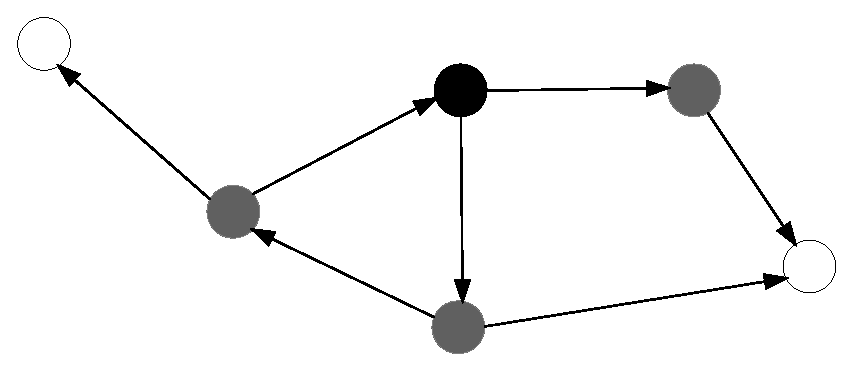
\includegraphics[width=\paperwidth,height=\paperheight,%
keepaspectratio]{figs/wNodeStatesBW.eps}%
\vfill
}}} 

%%%%%%%%%%%%%%%%%%%%%%%

% ## packages for graphics, etc ## ----------------------------------------------
%\usepackage[svgnames,pdf]{pstricks}
%\usepackage{pst-node}
%\usepackage{pst-tree}
\usepackage{ipe}
% following has problems with older ipe
% \usepackage{auto-pst-pdf} % pdflatex -shell-escape 
% need to use dvipdf and possibly trim margins manually
\usepackage{graphicx}
\DeclareGraphicsExtensions{.pdf,.png,.eps}
\graphicspath{{figs/}} 
%\usepackage{epsfig} % <- outdated, use something else   


% ## fonts ## ----------------------------------------------
\usepackage{amsmath}
\usepackage{amssymb}
\usepackage{amsthm}
\usepackage{newtxmath} % Times New Roman math font

\usepackage{utopia}
\newcommand{\defnfont}[1]{\textbf{\textit{#1}}\index{#1}}
\newcommand{\boldfont}[1]{\emph{#1}}
\newcommand{\algfont}[1]{\texttt{#1}\index{algorithm!#1}}

%\input Sanremo.fd
%\newcommand{\CAP}[1]{\mbox{\usefont{U}{Sanremo}{xl}{n}\selectfont #1}}
\input Starburst.fd      % weird star font
\newcommand{\CAP}[1]{\mbox{\usefont{U}{Starburst}{xl}{n}\selectfont #1}}


% ## style ## ----------------------------------------------
\renewcommand{\labelitemii}{$\circ$}
% roman letters in enumerate
\makeatletter
\def\romenumi{
\def\theenumi{\roman{enumi}}
\def\p@enumi{\theenumi}
\def\labelenumi{(\@roman\c@enumi)}}
\makeatother


% ## math theorems ----------------------------------------------
\theoremstyle{definition}
\newtheorem{Lemma}{Lemma}
\newtheorem{Theorem}[Lemma]{Theorem}
\newtheorem{Definition}[Lemma]{Definition}
\newtheorem{Corollary}[Lemma]{Corollary}
\newtheorem{Example}[Lemma]{Example}
\newtheorem{Exercise}{Exercise}

\numberwithin{Lemma}{chapter}
\numberwithin{Exercise}{section}

\theoremstyle{remark}

\newtheorem*{note}{Note}
\newtheorem*{statement}{Statement}
\newtheorem*{theorem}{Theorem}
\newtheorem*{tech}{\textbf{Technique}}

\newtheoremstyle{boxampleStyle}
  {0pt} % measure of space to leave above the theorem.
  {\topsep} % measure of space to leave below the theorem.
  {\normalfont} % name of font to use in the body of the theorem.
  {0pt} % measure of space to indent.
  {\bfseries} % name of head font.
  {. } % punctuation between head and body.
  { } % space after theorem head.
  {} %
\theoremstyle{boxampleStyle} 
\newtheorem{ExampleInBox}[Lemma]{Example}

\usepackage{mdframed}
\usepackage{xparse}
\NewDocumentEnvironment{Boxample}{o}{%
    \begin{mdframed}\begin{ExampleInBox}%
}{%
    \end{ExampleInBox}%
    \vspace*{#1cm}%
    \end{mdframed}%
}

% \newcommand{\truevspace}[1]{ %Call this macro to get a vertical space of #1 cm
% \newcount\Scount
% \Scount=0
% \loop\vspace*{1cm}\par\goodbreak\advance\Scount by 1 \ifnum\Scount< #1 \repeat
% }
% \def\beginboxedexample{\begin{mdframed}\begin{Example}}
% \def \endboxedexample #1 {\vspace{#1} \end{Example} \end{mdframed} }


% ## definitions & macros ## ----------------------------------------------
\newcommand{\set}[1]{\mbox{$\{#1\}$}}
\newcommand{\solution}[1]%
{\medskip \noindent{\textsc{\textbf{Solution to \cref{#1} on
page~\pageref{#1}}}}:\newline }

\usepackage{mathtools}
\DeclarePairedDelimiter\abs{\lvert}{\rvert}

% ## Algos ## ----------------------------------------------
\newcommand{\AlgCmt}[1]{\psframebox[linecolor=lightgray]{\ #1\ }}
\newcommand{\AdjLists}[1]{\psframebox[linecolor=lightgray]{\ #1\ }}

\newcommand{\Algorbody}[1]{
\begin{tabbing}
xxxx\=xxxx\=xxxx\=xxxx\=xxxx\=xxxx\=xxxx\= \kill

#1
\end{tabbing}
}

\newcommand{\Algorithm}[4]{ 
\begin{tabbing}
xxxx\=xxxx\=xxxx\=xxxx\=xxxx\=xxxx\=xxxx\= \kill
\textbf{algorithm } \algfont{#1} \\
\> {\textit{\textbf{Input: }} #2}\\
\textbf{begin} \\
#4
\textbf{end}
\end{tabbing}
} 


% ## refs ## ----------------------------------------------
\usepackage[colorlinks,linkcolor=blue,urlcolor=blue,citecolor=blue,
 bookmarksopen=true,
 pdfauthor={David Welch, Mark C. Wilson, Jonathan Klawitter}, 
 pdfsubject={Coursebook},
 pdftitle={CS220 Algorithms and Data Structures},
 pdfcreator={LaTeX with hyperref package},
 pagebackref=true,
]{hyperref}
\usepackage[capitalise,noabbrev,nameinlink ]{cleveref} 


% headings hacked from memoir package
\makeatletter
\makepagestyle{220book}
\setlength{\headwidth}{1.1\textwidth}
\makerunningwidth{220book}{\headwidth}
\makeheadrule{220book}{\headwidth}{\normalrulethickness}
\makeheadposition{220book}{flushright}{flushleft}{}{}
\makepsmarks{220book}{%
  \let\@mkboth\markboth
  \def\chaptermark##1{%
        \markboth{{%\MakeUppercase{%
          \ifnum \c@secnumdepth >\m@ne
            \if@mainmatter
              \@chapapp\ \thechapter: \ %
            \fi
          \fi
          ##1}}{}}%
  \def\sectionmark##1{\markright{%
    \ifnum \c@secnumdepth>\z@
      Section~\thesection: \ %
    \fi
    ##1}}
  \def\tocmark{\markboth{\contentsname}{\contentsname}}
  \def\lofmark{\markboth{\listfigurename}{\listfigurename}}
  \def\lotmark{\markboth{\listtablename}{\listtablename}}
  \def\bibmark{\markboth{\bibname}{\bibname}}
 \def\indexmark{\markboth{\indexname}{\indexname}}
}
\makeevenhead{220book}
{{\normalfont\large\bfseries\thepage} \quad \footnotesize\rightmark}
{} {}
\makeoddhead{220book}{}{}%
{\footnotesize\leftmark \quad {\normalfont\large\bfseries\thepage}}
\makeatother
\makeevenfoot{plain}{}{}{}
\makeoddfoot{plain}{}{}{}

\includeonly{
%intro/intro4,
%intro/intro3,
%intro/intro2,
%intro/intro,
%algorithm-analysis/alg-anal, 
%algorithm-analysis/sort,
%algorithm-analysis/search, 
lectures/graph-adt, 
lectures/traversal, 
%lectures/optimization,
%automata-grammars/automata,  % e-book excluded
%automata-grammars/grammars,
%appendix/javagraphADT,
%appendix/javasortmeth,
%appendix/javaparse,
%appendix/datastruct,
%appendix/mathfacts,
%appendix/solutions,
%reference/reference
}


% --- ### BEGIN DOCUMENT ### ---
\begin{document}   


% # title page
%\AddToShipoutPicture*{\BackgroundPic}

\pagestyle{220book}

\if 11
\title{\color{white}\textbf{\CAP Introduction to \CAP Algorithms and \CAP Data \CAP Structures}}
\author{\color{yellow}\textsc{Michael J. Dinneen ~~~ Georgy Gimel'farb ~~~ Mark C. Wilson}\\[4.6in]}
%\date{\color{white} February 2016\\[2ex] (4\textsuperscript{th} e-book edition)}
\date{\color{white} \copyright 2016\\[2ex] (Fourth edition)}
\maketitle
\else
\title{\textbf{Introduction to Algorithms and Data Structures}\\[4ex]}
\author{Michael J. Dinneen \\ Georgy Gimel'farb \\ Mark C. Wilson\\[3in]}
\date{February 2016\\[2ex] (4\textsuperscript{th} e-book edition)}

\begin{titlingpage}
\thispagestyle{empty}
\aliaspagestyle{titlingpage}{companion}
%\CenterWallPaper{vc6spiral.eps}
\maketitle
%\noindent\includegraphics[width=5.53in]{vc6spiral}
\end{titlingpage}
\fi % <- coursebook version

\author{David Welch, Mark C. Wilson, Jonathan Klawitter}
\title{CS220 Algorithms and Data Structures}
\date{\today}
\maketitle


% - ### front matter ### -
\setcounter{page}{1}

%\tableofcontents

%\newpage
%\listoffigures

%\newpage
%\listoftables


% - ### main matter ### -
%\mainmatter
\chapterstyle{ger}


%\part{Introduction to Algorithm Analysis}

\chapter{What is Algorithm Analysis?}  
\label{CH:ALG:ANAL}
%
\newcommand{\illustr}[2]{\centerline{\psfig{figure=figs/#1,width=#2}}}
  
Algorithmic problems are of crucial importance in modern life. 
Loosely speaking, they are precisely formulated problems that can be solved in a
step-by-step, mechanical manner. 

\begin{Definition}[informal]
An \defnfont{algorithm} is a list of unambiguous rules that specify successive 
steps to solve a problem. A  \defnfont{computer program} is a clearly specified 
sequence of computer instructions implementing the algorithm. 
\end{Definition}

For example, a sufficiently detailed recipe for making a cake could
be thought of as an algorithm. Problems of this sort are not normally
considered as part of computer science. In this book, we deal with algorithms 
for problems of a more abstract nature. Important examples, all discussed in this 
book, and all with a huge number of practical applications, include: sorting a 
database, finding an entry in a database, finding a pattern in a text document, 
finding the shortest path through a network, scheduling tasks as efficiently as 
possible, finding the median of a statistical sample.

Strangely enough, it is very difficult to give simple precise mathematical
definitions of algorithms and programs. The existing very deep general
definitions are too complex for our purposes. We trust that the reader
of this book will obtain a good idea of what we mean by algorithm from
the examples in this and later chapters.

We often wish to compare different algorithms for the same problem,
in order to select the one best suited to our requirements. The main
features of interest are: whether the algorithm is \defnfont{correct}
(does it solve the problem for all legal inputs), and how \emph{efficient} it 
is (how much time, memory storage, or other resources it uses).

The same algorithm can be implemented by very different programs written
in different programming languages, by programmers of different levels of skill,
and then run on different computer platforms under different operating systems.
In searching for the best algorithm, general features of algorithms must be 
isolated from peculiarities of particular platforms and programs. 

To analyse computer algorithms in practice, it is usually sufficient to
first specify elementary operations of a ``typical'' computer and then
represent each algorithm as a sequence of those operations.

Most modern computers and languages build complex programs from
ordinary arithmetic and logical operations such as standard unary and
binary arithmetic operations (negation, addition, subtraction,
multiplication, division, modulo operation, or assignment), Boolean
operations, binary comparisons (``equals", ``less than", or
``greater than"), branching operations, and so on. It is quite natural
to use these basic computer instructions as algorithmic operations,
which we will call \defnfont{elementary operations}.

It is not always clear what should count as an elementary operation. For
example, addition of two 64-bit integers should definitely count
as elementary, since it can be done in a fixed time for a given
implementation. But for some applications, such as cryptography, we must
deal with much larger integers, which must be represented in another
way. Addition of ``big" integers takes a time roughly proportional to
the size of the integers, so it is not reasonable to consider it as
elementary. From now on we shall ignore such problems. For most of the
examples in this introductory book they do not arise. However, they must
be considered in some situations, and this should be borne in mind.

\begin{Definition} [informal]
The \defnfont{running time} (or computing time) of an algorithm
is the number of its elementary operations.
\end{Definition}

The actual execution time of a program implementing an algorithm is
roughly proportional to its running time, and the scaling factor depends
only on the particular implementation (computer, programming language,
operating system, and so on).

The memory space required for running an algorithm depends on how many individual
variables (input, intermediate, and output data) are involved
simultaneously at each computing step. Time and space requirements
are almost always independent of the programming language or style and
characterise the algorithm itself. From here on, we will measure
effectiveness of algorithms and programs mostly in terms of their time
requirements. Any real computer has limits on the size and the number of
data items it can handle.

\section{Efficiency of algorithms: first examples}
\label{sec:efficiency}

If the same problem can be solved by different algorithms, then all other
things being equal, the most efficient algorithm uses least computational
resources. The theory of algorithms in modern computer science clarifies
basic algorithmic notions such as provability, correctness, complexity,
randomness, or computability. It studies  whether there exist any
algorithms for solving certain problems, and if so, how fast can they
be. In this book, we take only a  few small steps into this domain.

To search for the most efficient algorithm, one should mathematically
prove correctness of and determine time/space resources for each
algorithm as explicit functions of the size of input data to process.
For simplicity of presentation in this book, we sometimes skip the first 
step (proof of correctness), although it is very important. The focus of this 
chapter is to introduce methods for estimating the resource requirements of 
algorithms.

\begin{Example}[Sum of elements of an array]
\label{ex:lin:sum} 
Let $a$ denote an array of integers where the sum
\(
s = \sum_{i=0}^{n-1} a[i]
\) is required.
To get the sum \(s\), we have to repeat \(n\) times  
the same elementary operations (fetching 
from memory and adding a number). Thus, running time $T(n)$
is proportional to, or \emph{linear} in $n$: 
\( T(n) = c  n \). Such
algorithms are also called \defnfont{linear algorithms}. The unknown  
factor $c$ depends on a particular computer, 
programming language, compiler, operating system, etc. But 
the relative change in running time is 
just the same as the change in the data size:  
$T(10) = 10  T(1)$, or $T(1000) = 1000  T(1)$, 
or $T(1000)=10 T(100)$. The linear 
algorithm in Figure~\ref{fig:alg-linsum} implements a simple loop.

\begin{figure}
\hspace*{1.2in}\begin{minipage}{5in}
\Algorithm{linearSum}{array $a[0..n-1]$}{the sum \(s\)}
{
\> \(s \leftarrow 0\)\\
\> \textbf{for} \(i \leftarrow  0\) \textbf{step} \(i \leftarrow i+1\)
                            \textbf{until} \(n-1\) \textbf{do}\\
\> \> \(s \leftarrow s + a[i] \) \\
\> \textbf{end for} \\
\> \textbf{return} $s$\\
}
\end{minipage}
\caption{Linear-time algorithm to sum an array.}
\label{fig:alg-linsum}
\end{figure}

\end{Example}

\begin{Example} [Sums of subarrays]
\label{ex:con:subseq} 
The problem is to compute, for each subarray
$a[j..j+m-1]$ of size \(m\) in an array
$a$ of size \(n\), the partial sum of its elements $s[j]= 
\sum_{k=0}^{m-1}a[j+k]$; \(j=0,\ldots,n-m\). The total number of these
subarrays is \(n-m+1\). At first glance, we need to compute
\(n-m+1\) sums, each  of $m$ items, so that the running time is
proportional to $m  (n-m+1)$. If $m$ is fixed, the time depends still
linearly on $n$.

But if \(m\) is growing with $n$ as
a fraction of \(n\), such as \(m=\frac{n}{2}\), 
then 
\(
T(n) = c  \frac{n}{2}  \left(\frac{n}{2}+1\right)\) \( = 
0.25cn^{2} + 0.5cn 
\). 
The relative weight of the linear part, \(0.5cn\), 
decreases quickly with respect to the quadratic one
as $n$ increases. For example, if \(T(n) = 0.25n^{2} + 0.5n\), we see in 
the last column of Table~\ref{table:quad-beats-lin} the rapid decrease of the 
ratio of the two terms.

\begin{table}[hbtp]
\caption{Relative growth of linear and quadratic terms in an expression.}
\label{table:quad-beats-lin}
\begin{center}
\begin{tabular}{|r|r|r|r|r|} \hline
$n$ & $T(n)$ & $0.25n^{2}$ & \multicolumn{2}{c|}{$0.5n$}\\ \cline{4-5}
    &        &             & \textbf{value} & \% of quadratic term \\ \hline
10  & 30     &  25  & 5  & 20.0\\
50  & 650    & 625  & 25 & 4.0\\
100 & 2550   & 2500 & 50 & 2.0\\ 
%\end{tabular}
%\begin{tabular}{|r|r|r|r|r|} \hline
%$n$ & $T(n)$ & $0.25n^{2}$ & \multicolumn{2}{c|}{$0.5n$}\\ \cline{4-5}
%    &        &             & \textbf{value} & \% \\ \hline
500 & 62750  & 62500 & 250 & 0.4\\
1000& 250500 &250000 & 500 & 0.2\\ 
5000& 6252500&6250000&2500 & 0.04\\\hline
\end{tabular}
\end{center}
\end{table}

Thus, for large $n$ only the quadratic term becomes important
and the running time is roughly proportional to $n^{2}$,
or is quadratic in $n$. Such algorithms are sometimes called
\defnfont{quadratic algorithms} in terms of relative changes of running time with
respect to changes of the data size: if \(T(n) \approx cn^2\) then $T(10)
\approx 100 T(1)$, or $T(100) \approx 10000 T(1)$, or $T(100) \approx
100 T(10)$.


\begin{figure}[htbp]
\begin{center}
\begin{minipage}{5in}
\Algorithm{slowSums}
{array $a[0..2m-1]$}
{array $s$ of size \(m+1\)}
{
\> array $s[0..m]$\\
\> \textbf{for} \(i \leftarrow  0\) \textbf{to} $m$ \textbf{do}\\
\> \>\(s[i] \leftarrow 0\)\\
\> \>\textbf{for} \(j \leftarrow  0\) \textbf{to} \(m-1\) \textbf{do}\\
\> \>\>\(s[i] \leftarrow s[i] + a[i+j] \) \\
\> \>\textbf{end for} \\
\> \textbf{end for} \\
\> \textbf{return} $s$ \\
}
\end{minipage}
\end{center}
\caption{Quadratic time algorithm to compute sums of an array.}
\label{fig:alg-bad-array-sum}
\end{figure}

The ``brute-force'' quadratic algorithm has two nested loops (see
Figure~\ref{fig:alg-bad-array-sum}).
Let us analyse it to find out whether it can be simplified. It is easily
seen that repeated computations in the innermost loop are unnecessary.
Two successive sums $s[i]$ and $s[i-1]$ differ only by
two elements: \(s[i]=s[i-1]+ a[i+m-1]-a[i-1]\). Thus we need not
repeatedly add $m$ items together after getting the very first sum
$s[0]$. Each next sum is formed from the current one by using only two
elementary operations (addition and subtraction). Thus $T(n) = c  (m + 2
 (n-m)) = c  (2n - m)$. In the first parentheses, the first term $m$
relates to computing the first sum $s[0]$, and the second term $2 
(n-m)$ reflects that $n-m$ other sums are computed with only two
operations per sum. Therefore, the running time for this better
organized computation is always linear in $n$ for each value $m$, either
fixed or growing with $n$. The time for computing all the sums of the
contiguous subsequences is less than twice that taken for the single sum of all 
$n$ items in Example~\ref{ex:lin:sum}
 
The linear algorithm in Figure~\ref{fig:alg-good-array-sum}
excludes the innermost loop of the quadratic
algorithm. Now two simple loops, doing $m$ and $2(n-m)$ elementary
operations, respectively, replace the previous nested loop performing $m
 (n-m+1)$ operations. 
\end{Example} 

\begin{figure}[hbtp]
\begin{center}
\begin{minipage}{5in}
\Algorithm{fastSums}
{array $a[0..2m-1]$}
{array $s$ of size \(m+1\)}
{
\> array $s[0..m]$\\
\> \(s[0] \leftarrow 0\) \\
\> \textbf{for} \(j \leftarrow  0\) \textbf{to} \(m-1\) \textbf{do}\\
\> \>\(s[0] \leftarrow s[0] + a[j] \) \\
\> \textbf{end for} \\
\> \textbf{for} \(i \leftarrow  1\) \textbf{to} \(m\) \textbf{do}\\
\> \>\(s[i] \leftarrow s[i-1] + a[i+m-1]- a[i-1] \) \\
\> \textbf{end for} \\
\> \textbf{return} $s$;\\
}
\end{minipage}
\end{center}
\caption{Linear-time algorithm to compute sums of an array.}
\label{fig:alg-good-array-sum}
\end{figure}

Such an outcome is typical for algorithm analysis. In many cases, a
careful analysis of the problem allows us to replace a straightforward
``brute-force'' solution with much more effective one. But there are no
``standard'' ways to reach this goal. To exclude unnecessary
computation, we have to perform a thorough investigation of the problem
and find hidden relationships between the input data and desired
outputs. In so doing, we should exploit  all the tools we have learnt.
This book presents many examples where analysis tools are indeed useful,
but knowing how to analyse and solve each particular problem is still close to
an art. The more examples and tools are mastered, the more the art is
learnt. 

\subsection*{Exercises}

\begin{Exercise}
\label{exr:time-compl:2}
A quadratic algorithm with processing time \(T(n)=cn^2 \)
uses 500 elementary operations for processing $10$ data items. How many will it 
use for processing $1000$ data items? 
\end{Exercise}


\begin{Exercise}
\label{exr:time-compl:7A}
Algorithms \textbf{A} and 
\textbf{B} use
exactly \(T_\mathrm{A}(n) = c_\mathrm{A} n \lg n\)
and \(T_\mathrm{B}(n) = c_\mathrm{B} n^{2}\) elementary operations, 
respectively, for a problem of size \(n\).
Find the fastest algorithm for processing \(n=2^{20}\) data items if
\textbf{A} and \textbf{B} spend 10 and 1 operations,
respectively, to process \(2^{10}\equiv 1024\) items.
\end{Exercise}

\section{Running time for loops and other computations}
\label{rt-loops}

The above examples show that running time depends considerably on how
deeply the loops are nested and how the loop control variables are
changing. Suppose the control variables change linearly in $n$, that
is, increase or decrease by constant steps. If the number of elementary
operations in the innermost loop is constant, the nested loops result
in polynomial running time $T(n) = c  n^{k}$ where $k$ is
the highest level of nesting and $c$ is some constant. The first three
values of $k$ have special names: \defnfont{linear time}, 
\defnfont{quadratic time},
and \defnfont{cubic time} for $k=1$ (a single loop), $k=2$ (two nested
loops), and $k=3$ (three nested loops), respectively.

When loop control variables change non-linearly,
the running time also varies non-linearly with $n$.

\begin{Example} 
An exponential change \(i=1,k,k^2 ,\ldots, k^{m-1}\) of
the control variable  in the
range \(1 \le i \le n\) results in \defnfont{logarithmic time}
for a simple loop. The loop executes $m$ 
iterations such that $k^{m-1} \le  n  < k^{m}$. Thus, $m-1 \le \log_{k} n
< m$, and $T(n) = c  \lceil \log_{k} n \rceil$.
\end{Example}
 
Additional conditions for executing inner loops only for special values of 
the outer variables also decrease running time. 

\begin{Example} 
\label{exm:nest2}
Let us roughly estimate the running time of the following nested loops:
 
\hspace*{.3in}\begin{minipage}{5in}
\Algorbody
{
\(m \leftarrow 2\) \\
\textbf{for} \(j \leftarrow 1\) \textbf{to} \(n\) \textbf{do}\\
\>\textbf{if} \(j = m \) \textbf{then} \\
\>\> \(m \leftarrow 2m\) \\
\>\>\textbf{for} \(i \leftarrow  1\) \textbf{to} \(n\) \textbf{do}\\
\>\>\>$\ldots$ \AlgCmt{constant number of elementary operations} \\
\>\>\textbf{end for} \\
\>\textbf{end if}\\
\textbf{end for}\\
}
\end{minipage}

The inner loop is executed $k$ times for $j=2, 4, \ldots, 2^{k}$
where $k < \lg n \le k+1$. The total time for the elementary operations is 
proportional to $kn$, that is, $T(n)=  n  \lfloor \lg n \rfloor$.    
\end{Example}



Conditional and switch operations like \textbf{if}
\{\emph{condition}\} \textbf{then} \{\emph{constant running time}
$T_1$\} \textbf{else} \{\emph{constant running time} $T_2$\} involve
relative frequencies of the groups of computations.  The running time
$T$ satisfies $T = f_\mathrm{true} T_1 + (1 - f_\mathrm{true}) T_2 <
\max \{ T_1, T_2 \}$ where $f_\mathrm{true}$ is the relative frequency
of the true condition value in the if-statement.

The running time of a function or method call is $T = \sum_{i=1}^{k}T_i$
where $T_i$ is the running time of statement \(i\) of the function
and $k$ is the number of statements.


\subsection*{Exercises}

\begin{Exercise}
\label{exm:nest1}
Is the running time quadratic or linear for the nested loops below?\\

\begin{minipage}{5in}
\Algorbody
{
\(m \leftarrow 1\) \\
\textbf{for} \(j \leftarrow 1\) \textbf{step} \(j \leftarrow j+1\) 
                                    \textbf{until} \(n\) \textbf{do}\\
\>\textbf{if} \(j = m \) \textbf{then} \(m \leftarrow m \cdot (n-1)\) \\
\>\>\textbf{for} \(i \leftarrow  0\) \textbf{step} \(i \leftarrow i+1\) 
                                       \textbf{until} \(n-1\) \textbf{do}\\
\>\>\>$\ldots$ \AlgCmt{constant number of elementary operations} \\
\>\>\textbf{end for} \\
\>\textbf{end if}\\
\textbf{end for} \\
}
\end{minipage}

\end{Exercise}

\begin{Exercise}
\label{ex:nest2}

What is the running time for the following code fragment as a function of $n$?
\begin{center}
\begin{minipage}{5in}
\Algorbody
{
\textbf{for} $i \gets 1$ \textbf{step} $i \gets 2*i$ \textbf{while} $i<n$ \textbf{do} \\
\> \textbf{for} $j \gets 1$ \textbf{step} $j \gets 2*j$ \textbf{while} $j<n$ \textbf{do} \\
\> \> \textbf{if} $j = 2*i$ \\
\> \> \> \textbf{for} $k = 0$ \textbf{step} $k\gets k+1$ \textbf{while} $k<n$ \textbf{do} \\
\> \> \> \> $\ldots$ \AlgCmt{constant number of elementary operations} \\
\>\>\> \textbf{end for}\\
\> \> \textbf{else} \\
\> \> \> \textbf{for} $k \gets 1$ \textbf{step} $k\gets 3*k$ \textbf{while} $k<n$ \textbf{do} \\
\> \> \> \> $\ldots$ \AlgCmt{constant number of elementary operations} \\
\>\>\> \textbf{end for}\\
\>\> \textbf{end if} \\
\> \textbf{end for} \\
\textbf{end for}
}
\end{minipage}
\end{center}
\end{Exercise}

\section{``Big-Oh'', ``Big-Theta'', and ``Big-Omega'' tools} \label{tools}

Two simple concepts separate properties of an algorithm itself from
properties of a particular computer, operating system, programming
language, and compiler used for its implementation. The concepts,
briefly outlined earlier, are as follows: 
\begin{itemize}
 \item The \defnfont{input data size}, or
the number $n$ of individual data items in a single data instance to be
processed when solving a given problem. Obviously, how to measure the data
size depends on the problem: \(n\) means the number of items to sort (in sorting
applications),
number of nodes (vertices) or arcs (edges) in graph algorithms, number
of picture elements (pixels) in image processing, length of a character
string in text processing, and so on.  
\item The number of elementary operations taken by a particular algorithm, or its
running time. We assume it is a function $f(n)$ of the input data size
$n$. The function depends on the elementary operations chosen to build the
algorithm. 
\end{itemize} 

The running time of a program which implements
the algorithm is $c  f(n)$ where $c$ is a constant factor depending
on a computer, language, operating system, and compiler. Even if we don't know 
the value of the factor \(c\), we are able to answer the important question:
\emph{if the input size increases from $n=n_{1}$ to $n=n_{2}$, how does
the relative running time of the program change, all other things being equal?}
The answer is obvious: the 
running time increases by a factor of 
\( 
\frac{T(n_{2})}{T(n_{1})} = 
\frac{c  f(n_{2})}{c  f(n_{1})} =  
\frac{f(n_{2})}{f(n_{1})}
\). 

As we have already seen, the approximate running time for large input
sizes gives enough information to distinguish between a good and a bad
algorithm. Also, the constant $c$ above can rarely be determined. We
need some mathematical notation to avoid having to say ``\emph{of the
order of} $\ldots$''  or ``\emph{roughly proportional to} $\ldots$'',
and to make this intuition precise.

The standard mathematical tools ``\emph{Big Oh}'' ($O$), ``\emph{Big
Theta}'' ($\Theta$), and ``\emph{Big Omega}'' ($\Omega$) do 
precisely this.

\begin{note}
Actually, the above letter $O$ is a capital ``omicron''  (all
letters in this notation are Greek letters). However, since the Greek
omicron and the English ``O'' are indistinguishable in most fonts, we
read $O()$ as ``Big Oh'' rather than ``Big Omicron''. 
\end{note}

The algorithms are analysed under the following assumption: \emph{if
the running time of an algorithm as a function of $n$ differs only by a
constant factor from the  running time for another algorithm, then the
two algorithms have essentially the same running time.} Functions that
measure running time, $T(n)$, have nonnegative values because time is
nonnegative, $T(n) \ge 0$. The integer argument $n$ (data size) is also
nonnegative.

\begin{Definition} [Big Oh]
\label{def:oh}
Let $f(n)$ and $g(n)$ be nonnegative-valued functions defined on
nonnegative integers $n$. Then $g(n)$ is $O(f(n))$ (read ``\(g(n)\) is
Big Oh of \(f(n)\)'') iff there exists 
a positive real constant $c$ and
a positive integer $n_{0}$ such that $g(n) \le c f(n)$ for all $n>n_{0}$.
\end{Definition}
\begin{note} 
We use the notation ``\defnfont{iff}'' as an abbreviation of ``if and only if''.
\end{note}
In other words, if $g(n)$ is $O(f(n))$ then an algorithm with running time 
$g(n)$ runs for large $n$ at least as fast, to within a
constant factor, as an algorithm with running time  $f(n)$. Usually
the term ``\defnfont{asymptotically}'' is used in this context to describe 
behaviour of functions for sufficiently large values of $n$. This term 
means that \(g(n)\) for large \(n\) may approach closer and closer to 
\(c\cdot f(n)\). Thus, \(O(f(n))\) specifies
an \defnfont{asymptotic upper bound}.
\begin{note} 
Sometimes the ``Big Oh'' property is denoted $g(n)=O(f(n))$, but
we should not assume that the function $g(n)$ is equal to something 
called ``Big Oh'' of $f(n)$. This notation really means $g(n) \in O(f(n))$, 
that is, \(g(n)\) is a member of the set $O(f(n))$ 
of functions which are increasing, in essence, with the same 
or lesser rate as  \(n\) tends to infinity ($n \rightarrow \infty$). 
In terms of graphs of these functions, $g(n)$ is $O(f(n))$ iff
there exists a constant $c$ such that the graph of $g(n)$ is always
below or at the graph of $cf(n)$ after a certain point, $n_{0}$. 
\end{note}

\begin{Example}
Function \(g(n)=100\log_{10}n\) in Figure~\ref{f:aa-graphs} 
is \(O(n)\) because the graph \(g(n)\) is always below
the graph of \(f(n)=n\) if \(n > 238\) or of \(f(n)=0.3n\)
if \(n > 1000\), etc. 
\end{Example}

\begin{figure}[htb!]
\centerline{
\illustr{aa-graphs.eps}{80mm}}
\caption{``Big Oh'' property: $g(n)$ is $O(n)$.}
\label{f:aa-graphs}
\end{figure}
\begin{Definition} [Big Omega]
\label{def:omega}
The function $g(n)$ is $\Omega(f(n))$ iff 
there exists a positive real constant $c$ and a 
positive integer $n_{0}$  
such that $g(n) \ge c f(n)$ for all $n>n_{0}$.
\end{Definition} 

``Big Omega'' is complementary to ``Big Oh'' and generalises the
concept of ``lower bound'' (\(\ge\)) in the same way as ``Big Oh''
generalises the concept of ``upper bound'' (\(\le\)): if
\(g(n)\) is \(O(f(n))\) then \(f(n)\) is \(\Omega(g(n))\), and vice versa. 

\begin{Definition} [Big Theta]
\label{def:theta}
The function $g(n)$ is $\Theta(f(n))$ iff 
there exist two positive real constants $c_1$ and $c_2$ and a 
positive integer $n_{0}$  
such that $c_1f(n) \le g(n) \le c_2 f(n)$ for all $n>n_{0}$.
\end{Definition}

Whenever two functions, \(f(n)\) and \(g(n)\), are actually of the same
order, \(g(n)\) is \(\Theta(f(n))\), they are each ``Big Oh'' of the
other: $f(n)$ is $O(g(n))$ and $g(n)$ is  $O(f(n))$. In other words,
\(f(n)\) is both an asymptotic upper and lower bound for \(g(n)\). The
``Big Theta'' property means \(f(n)\) and \(g(n)\) have asymptotically
tight bounds and are in some sense equivalent for our purposes.

In line with the above definitions,
\(g(n)\) is \(O(f(n))\) iff \(g(n)\) grows \boldfont{at 
most} as fast as \(f(n)\) to within a constant factor, \(g(n)\) is
\(\Omega(f(n))\) iff \(g(n)\) grows \boldfont{at 
least} as fast as \(f(n)\) to within a constant factor, and
\(g(n)\) is \(\Theta(f(n))\) iff \(g(n)\) and \(f(n)\) grow
\boldfont{at the same rate} to within a constant factor.


``Big Oh'', ``Big Theta'', and ``Big Omega'' notation formally capture 
two crucial ideas in comparing algorithms:
the exact function, $g$, is not very
important because it can be multiplied by any
arbitrary positive constant, $c$, and
the relative behaviour of two functions
is compared only asymptotically, for large $n$, but not near the
origin where it may make no sense.
Of course, if the constants involved are very large, 
the asymptotic behaviour loses practical interest. In most
cases, however, the constants remain fairly small. 

In analysing running time,
``Big Oh'' $g(n) \in O(f(n))$, ``Big Omega'' $g(n) \in \Omega(f(n))$,
and ``Big Theta'' $g(n) \in \Theta(f(n))$  
definitions are mostly used with $g(n)$ equal to 
``exact'' running time on inputs of size $n$ and 
$f(n)$ equal to a rough approximation to
running time (like \(\log n\), \(n\), \(n^2\), and so on).
 
To prove that some
function \(g(n)\) is \(O(f(n))\), \(\Omega(f(n))\), or 
\(\Theta(f(n))\) using the definitions we need to find the constants \(c\), \(n_0\) or \(c_1\), \(c_2\), \(n_0\) specified in 
Definitions~\ref{def:oh}, \ref{def:omega}, \ref{def:theta}. 
Sometimes the proof is given only by a chain of inequalities,
starting with \(f(n)\). In other cases it
may involve more intricate techniques, such as mathematical
induction. Usually the manipulations
are quite simple. To prove that \(g(n)\) is \boldfont{not} 
\(O(f(n))\), \(\Omega(f(n))\), or \(\Theta(f(n))\) we have 
to show the desired constants do not exist, that is,
their assumed existence leads to a contradiction.

\begin{Example}
To prove that 
linear function $g(n) = an + b$; $a > 0$, is $O(n)$, we
form the following chain of inequalities:  
\(g(n) \le an + |b| \le (a+|b|)n\) for all \(n \ge 1\).
Thus, Definition~\ref{def:oh}
with \(c=a+|b|\) and \(n_0 = 1\) shows 
that \(an + b\) is \(O(n)\). 
\end{Example} 
 
``Big Oh'' hides constant factors so that both $10^{-10}n$ and
$10^{10}n$ are $O(n)$. It is pointless to write something like  $O(2 
n)$ or $O(a  n + b)$ because this still means $O(n)$. Also, only 
the dominant terms as  $n \rightarrow
\infty$ need be shown as the argument of ``Big Oh'', ``Big Omega'', or
``Big Theta''.

\begin{Example} 
    The polynomial $P_{5}(n) = a_{5}n^{5} + a_{4}n^{4}+a_{3}n^{3} 
+a_{2}n^{2}+a_{1}n +a_{0}$; $a_{5}>0$, is $O(n^{5})$ 
because  
\(P_{5}(n) \leq (a_{5}+|a_{4}|+|a_{3}|+|a_{2}|+|a_{1}|+|a_{0}|)n^{5}\)
for  all \(n \ge 1\). 
\end{Example}


\begin{Example} 
\label{ex:expons}
The exponential function $g(n) = 2^{n+k}$, where $k$ is a constant,
is $O(2^{n})$ because 
\(2^{n+k} = 2^{k}  2^{n}\) for all \(n\).
Generally, $m^{n+k}$ is $O(l^{n})$; $l \ge m > 1$, because 
$m^{n+k} \le l^{n+k} = l^{k}  l^{n}$ for any constant $k$. 
\end{Example}

\begin{Example} 
\label{ex:logs}
For each $m>1$, the logarithmic function $g(n) = \log_{m}(n)$ has the same rate of 
increase as $\lg(n)$ because 
\(\log_{m}(n) = \log_{m}(2)  \lg(n)\) for  all \(n > 0\).
Therefore we may omit the logarithm base when using 
the ``Big-Oh'' and ``Big Theta'' notation: \(\log_{m}n\) is \(\Theta(\log n)\).
\end{Example}


\subsection{Rules for asymptotic notation}
\label{o-features}
 
Using the definition to prove asymptotic relationships between functions is hard
work. As in calculus, where we soon learn to use various rules (product rule, 
chain rule, \dots) rather than the definition of derivative, we can use some 
simple rules to deduce new relationships from old ones.

We present rules for ``Big Oh"---similar relationships hold for ``Big Omega'' 
and ``Big Theta''.

We will consider the features both informally and formally using the
following notation. Let $x$ and $y$ be functions of a nonnegative
integer $n$. Then $z=x+y$ and $z=xy$ denote the sum of the functions,
$z(n) = x(n)+y(n)$, and the product function: $z(n) = x(n)y(n)$,
respectively, for every value of $n$. The product function $(xy)(n)$
returns the product of the values of the functions at $n$ and has
nothing in common with the composition $x(y(n))$ of the two functions.

Basic arithmetic relationships for ``Big Oh''
follow from and can be easily proven with its definition. 

\begin{Lemma}[Scaling] \label{l:bigoh:1}
For all constants $c > 0$, $c  f$ is $O(f)$. In particular, $f$ is $O(f)$. 
\end{Lemma}

\begin{proof}
The relationship \(cf(n) \leq c f(n)\) obviously holds for all \(n\geq 0\).
\end{proof}

Constant factors are ignored, and only the powers and functions are
taken into account. It is this ignoring of constant factors that
motivates such a notation.

\begin{Lemma}[Transitivity] \label{l:bigoh:2}
If $h$ is $O(g)$ and $g$ is $O(f)$, then $h$ is $O(f)$.
\end{Lemma}
\begin{proof}
See Exercise~\ref{exr:bigoh:features}.
\end{proof}

Informally, if $h$ grows at most as quickly as $g$, which grows 
at most as quickly as $f$, then $h$ grows at most as quickly as $f$. 

\begin{Lemma}[Rule of sums] \label{l:bigoh:3}
%{\textsc{Rule of sums.}} 
If $g_{1}$ is $O(f_{1})$ and 
$g_{2}$ is $O(f_{2})$, then 
$g_{1}+g_{2}$ is $O(\max \{ f_{1},f_{2} \} )$. 
\end{Lemma}
\begin{proof}
See Exercise~\ref{exr:bigoh:features}.
\end{proof}

If $g$ is $O(f)$ and $h$ is $O(f)$, then is $g+h$ is $O(f)$. In particular, 
if $g$ is $O(f)$, then $g+f$ is $O(f)$. Informally, the growth rate of a sum 
is the growth rate of its fastest-growing term.
 
%\newpage 

\begin{Lemma}[Rule of products]\label{l:bigoh:4}
%{\textsc{Rule of products.}}
 If $g_{1}$ is $O(f_{1})$ and 
$g_{2}$ is $O(f_{2})$, then 
$g_{1}  g_{2}$ is $O(f_{1}  f_{2})$. 
\end{Lemma}
\begin{proof}
See Exercise~\ref{exr:bigoh:features}.
\end{proof}

In particular, if $g$ is $O(f)$, then $g  h$ is $O(f  h)$. Informally,
the product of upper bounds of functions gives an upper bound for the
product of the functions.

Using calculus we can obtain a nice time-saving rule.

\begin{Lemma}[Limit Rule] \label{l:bigoh:lim}
Suppose $\lim_{n\to \infty} f(n)/g(n)$ exists (may be $\infty$), and denote 
the limit by $L$. Then
\begin{itemize}
\item if $L=0$, then $f$ is $O(g)$ and $f$ is not $\Omega(g)$;
\item if $0 < L < \infty$ then $f$ is $\Theta(g)$;
\item if $L = \infty$ then $f$ is $\Omega(g)$ and $f$ is not $O(g)$.
\end{itemize}
\end{Lemma}

\begin{proof}
If $L = 0$ then from the definition of limit, in particular there is some 
$n_0$ such that $f(n)/g(n) \leq 1$ for all $n \geq n_0$. Thus $f(n) \leq g(n)$ 
for all such $n$, and $f(n)$ is $O(g(n))$ by definition. On the other 
hand, for each $c > 0$, it is not the case that $f(n) \geq c g(n)$ for all
$n$ past some threshold value $n_1$, so that $f(n)$ is not $\Omega(g(n))$.
The other two parts are proved in the analogous way.
\end{proof}

To compute the limit if it exists, the standard \emph{L'H\^{o}pital's rule}
of calculus is useful (see Section~\ref{sec:app:lhopital}).

More specific relations follow directly from the basic ones.

\begin{Example} 
\label{ex:powers}
Higher powers of $n$ grow more quickly than lower powers:
$n^{k}$ is $O(n^{l})$ if $0 \le k \le l$. This follows directly from the limit rule
since $n^k/n^l = n^{k-l}$ has limit $1$ if $k=l$ and $0$ if $k<l$.
\end{Example}

\begin{Example}  
The growth rate of a polynomial is given by the growth rate of its leading 
term (ignoring the leading coefficient by the scaling feature): 
if $P_{k}(n)$ is a polynomial of exact degree $k$ then $P_{k}(n)$ is $\Theta(n^{k})$. 
This follows easily from the limit rule as in the preceding example.
\end{Example}


\begin{Example}  
Exponential functions grow more quickly than powers: 
$n^{k}$ is $O(b^{n})$, for all $b>1$, $n>1$, and $k \ge 0$. 
The restrictions on $b$, $n$, and $k$ merely ensure that both 
functions are increasing. This result can be proved by induction or by using the 
limit-L'H\^{o}pital approach above.
\end{Example}

\begin{Example}  
Logarithmic functions grow more slowly than powers: 
$\log_{b} n$ is $O(n^{k})$ for all $b>1$, $k > 0$. 
This is the inverse of the preceding feature. Thus, 
as a result, $\log n$ is $O(n)$ and $n \log n$ is $O(n^{2})$.  
\end{Example} 

\subsection*{Exercises}

\begin{Exercise}\label{exr:aa:bigO:a}
Prove that $10n^3 - 5n + 15$ is not $O(n^{2})$.
\end{Exercise}
\begin{Exercise}\label{exr:aa:bigO:b}
Prove that $10n^3 - 5n + 15$ is $\Theta(n^{3})$.
\end{Exercise}
\begin{Exercise}\label{exr:aa:bigO:c}
Prove that $10n^3 - 5n + 15$ is not $\Omega(n^{4})$.
\end{Exercise}

\begin{Exercise}\label{exr:bigtheta}
Prove that $f(n)$ is $\Theta(g(n))$ if and only if both $f(n)$ is $O(g(n)$ and 
$f(n)$ is $\Omega(g(n))$.
\end{Exercise}

\begin{Exercise}
\label{exr:bigoh-order}
Using the definition, show that each function \(f(n)\) in 
Table~\ref{t:data-size} stands in ``Big-Oh'' relation to the preceding 
one, that is, \(n\) is \(O(n\log n)\), \(n\log n\) is \(O(n^{1.5})\),
and so forth. 

\end{Exercise}

\begin{Exercise}\label{exr:bigoh:features}
Prove Lemmas~\ref{l:bigoh:2}--\ref{l:bigoh:4}.
\end{Exercise}

\begin{Exercise}\label{exr:bigomega:sums}
Decide on how to reformulate the Rule of Sums (Lemma~\ref{l:bigoh:3})
for ``Big Omega'' and ``Big Theta'' notation.
\end{Exercise}

\begin{Exercise}\label{exr:bigomega:lem}
Reformulate and prove Lemmas~\ref{l:bigoh:1}--\ref{l:bigoh:4}
for ``Big Omega'' notation. 
\end{Exercise}

\section{running time of algorithms} 
\label{time-compl}

\begin{Definition} [Informal]
A function $f(n)$ such that the running time $T(n)$ of a given 
algorithm is $\Theta(f(n))$ measures the \defnfont{running time} 
of the algorithm.
\end{Definition}

An algorithm is called \defnfont{polynomial time} if its running time $T(n)$
is $O(n^{k})$ where $k$ is some fixed positive integer. A computational
problem is considered \defnfont{intractable} iff no deterministic
algorithm with polynomial running time exists for it. But many problems
are classed as intractable only because a polynomial solution is unknown,
and it is a very challenging task to find such a solution for one of them.
 
\begin{table}[htb] 
\caption[Relative growth of running time $T(n)$ when 
  the input size increases.]%
{\label{t:growth} Relative growth of running time $T(n)$ when 
  the input size increases from $n=8$ to $n=1024$ provided that $T(8)=1$.} 
  \centerline{
   \begin{tabular}{|c|c|cccc|c|} \hline 
   \multicolumn{2}{|c|}{\textbf{running time}} &  
   \multicolumn{4}{|c|}{\textbf{Input size $n$}} & \textbf{Time} $T(n)$
\\ \cline{1-6} 
   \emph{Function} & \emph{Notation} & \emph{8} & \emph{32} & \emph{128} & \emph{1024} &
\\ \hline 
   Constant     & $1$      & 1  & 1  &   1 &   1 & 1 \\ 
\hline 
   Logarithmic  & $\lg n$ & 1  & 1.67  & 2.67  & 3.33 & \( \lg n / 3 \)\\ 
\hline 
   Log-squared  & $\lg^{2} n$ & 1 & 2.78  & 5.44 &  11.1 & \( \lg^{2} n / 9 \) 
\\ \hline 
   Linear       & $n$ & 1 & 4 & 16 & 128 & \( n / 8 \) \\ 
\hline 
   ``$n\log n$''& $n \lg n$ & 1 & 6.67 & 37.3 & 427 & \(n \lg n / 24\)
\\ \hline 
   Quadratic    & $n^{2}$ & 1 & 16 & 256 & 16384 & \(n^{2} / 64\)
\\ \hline 
   Cubic        & $n^{3}$ & 1 & 64 & 4096 & 2097152 & \(n^{3} / 512\)
\\ \hline 
   Exponential  & $2^{n}$ & 1 & $2^{24}$ & $2^{120}$ & $2^{1016}$ & \(2^{n-8}\)
\\ \hline 
   \end{tabular}} 
 \end{table} 

Table~\ref{t:growth} shows how the running time \(T(n)\) of algorithms
having different running time, $f(n)$, grows relatively with the
increasing input size $n$.  running time functions are listed in
order such that $g$ is $O(f)$ if $g$ is above $f$: for example, the
linear function \(n\) is \(O(n\log n) \) and \(O(n^2 )\), etc. The 
asymptotic growth rate does not depend on the base of the logarithm, but the 
exact numbers in the table do --- we use $\log_{2} = \lg$ for simplicity.

\begin{table}[htbp] 
\caption[The largest data sizes $n$ that can be
processed by an algorithm.]%
{\label{t:data-size} The largest data sizes $n$ that can be
processed by an algorithm with running time $f(n)$
provided that $T(10)= 1$ minute.} 
\begin{center}
   \begin{tabular}{|c|r|r|r|r|r|r|} \hline
      & \multicolumn{6}{|c|}{\textbf{Length of time to run an algorithm}}\\
                \cline{2-7}
$f(n)$  & 1 minute & 1 hour & 1 day & 1 week & 1 year & 1 decade  \\
\hline
  $n$         & 10  & 600 & 14 400 & 100 800 & $5.26\times 10^{6}$  &
$5.26\times  10^{7}$  \\ \hline 
  $n\lg n$    & 10  & 250 & 3 997 & 23 100  & 883 895   & $7.64\times 10^6$
  \\ \hline 
  $n^{1.5}$    & 10  & 153 &  1 275 &   4 666 &    65 128 &
   302,409   \\ \hline 
  $n^{2}$      & 10  &  77 &    379 &   1 003 &     7 249 &
    22,932   \\ \hline 
  $n^{3}$      & 10  &  39 &    112 &     216 &       807 &
     1,738  \\ \hline 
  $2^{n}$      & 10  &  15 &     20 &      23 &        29 &
        32   \\ \hline
   \end{tabular}
   \end{center} 
 \end{table} 
 
Table~\ref{t:data-size} is even more expressive in showing
how the running time of an algorithm affects the size of problems the
algorithm can solve (we again use $\log_{2} = \lg$). A linear algorithm solving 
a problem of size $n=10$ in exactly one minute will process about $5.26$ million  
data items per year and 10 times more if we can wait a decade. 
But an exponential algorithm  with \(T(10)=1\) minute will deal
only with $29$ data items after a year of running and add only $3$
more items after a decade.  Suppose we have computers $10,000$ times
faster (this is approximately the ratio of a week to a minute). Then 
we can solve a problem $10,000$ times, $100$ times, or $21.5$ times 
larger than before if our algorithm is linear, quadratic, or cubic, 
respectively. But for exponential algorithms, our progress is much worse: 
we can add only $13$ more input values if $T(n)$ is $\Theta(2^n)$.

Therefore, if our algorithm has a constant, logarithmic, log-square, linear, 
or even ``$n \log n$'' running time we may be happy and start writing a 
program with no doubt that it will meet at least some practical demands. 
Of course, before taking the plunge, it is better to check whether the hidden 
constant $c$, giving the computation volume per data item, is sufficiently small
in our case. Unfortunately, order relations can be drastically
misleading: for instance, two linear functions $10^{-4}n$ and $10^{10}n$
are of the same order $O(n)$, but we should not claim an
algorithm with the latter running time as a big success.

Therefore, we should follow a simple rule: \emph{roughly estimate 
the computation volume per data item for the algorithms after comparing
their time complexities in a ``Big-Oh'' sense!} We may estimate the
computation volume simply by counting the number of elementary
operations per data item.

In any case we should be \boldfont{very} careful even with simple
quadratic or cubic algorithms, and especially with exponential
algorithms. If the running time is speeded up in Table~\ref{t:data-size} so that
it takes one \emph{second} per ten data items
in all the cases, then we will still wait about 12 \emph{days}
(\(2^{20}\equiv 1,048,576\) seconds) for processing only 30 items by the 
exponential algorithm. Estimate yourself whether it is
practical to wait until 40 items are processed.
 
In practice, quadratic and cubic algorithms cannot be used if the input
size exceeds tens of thousands or thousands of items, respectively,
and exponential algorithms should be avoided whenever possible unless we
always have to process data of very small size. Because even the most
ingenious programming cannot make an inefficient algorithm fast (we
would merely change the value of the hidden constant $c$ slightly, but
not the asymptotic order of the running time), it is better to spend
more time to search for efficient algorithms, even at the expense of a
less elegant software implementation, than to spend time writing a very
elegant implementation of an inefficient algorithm. 

\subsection{Worst-case and average-case performance}
\label{ss:worst-vs-avg}

We have introduced asymptotic notation in order to measure the running time of 
an algorithm. This is expressed in terms of elementary operations. ``Big Oh", 
``Big Omega" and ``Big Theta" notations allow us to state upper, lower
 and tight asymptotic bounds on running time that are independent of inputs and
implementation details. Thus we can classify algorithms by 
performance, and search for the ``best'' algorithms for solving a particular problem.  

However, we have so far neglected one important point. In general,
\emph{the running time varies not only according to the size of the
input, but the input itself}. The examples in Section~\ref{time-compl} 
were unusual
in that this was not the case. But later we shall see many examples
where it does occur. For example, some sorting algorithms take almost
no time if the input is already sorted in the desired order, but much
longer if it is not.

If we wish to compare two different algorithms for the same problem, it
will be very complicated to consider their performance on all possible
inputs. We need a simple measure of running time.

The two most common measures of an algorithm are the \defnfont{worst-case 
running time}, and the \defnfont{average-case running time}. 

The worst-case running time has several advantages.  If we can show,
for example, that our algorithm runs in time $O(n\log n)$ no matter
what input of size $n$ we consider, we can be confident that even if we
have an ``unlucky" input given to our program, it will not fail to run
fairly quickly. For so-called ``mission-critical" applications this is
an essential requirement. In addition, an upper bound on the worst-case
running time is usually fairly easy to find.

The main drawback of the worst-case running time as a measure is that it may be 
too pessimistic. The real running time might be much lower than
an ``upper bound'', the input data causing  the worst case may be
unlikely to be met in practice, and the constants $c$ and $n_{0}$ of the 
asymptotic notation  are unknown and may not be small.
There are many algorithms for which it is difficult to specify the worst-case 
input. But even if it is known, the inputs actually encountered in practice may 
lead to much lower running times. We
shall see later that the most widely used fast sorting
algorithm, quicksort, has worst-case quadratic
running time, $\Theta(n^{2})$, but its running time
for ``random" inputs encountered in practice is $\Theta(n \log n)$.

By contrast, the average-case running time is not as easy to define. The use of 
the word ``average" shows us that probability is involved. We need to specify a 
probability distribution on the inputs. Sometimes this is not too difficult. 
Often we can assume that every input of size $n$ is equally likely, and this 
makes the mathematical analysis easier. But sometimes an assumption of this sort
 may not reflect the inputs encountered in practice. Even if it does, the
average-case analysis may be a rather difficult mathematical challenge
requiring intricate and detailed arguments. And of course the worst-case 
complexity may be very bad even if the average case complexity is good, so there
 may be considerable risk involved in using the algorithm.

Whichever measure we adopt for a given algorithm, our goal is  to show
that its running time is $\Theta(f)$ for some function $f$ \boldfont{and}
there is no algorithm with running time $\Theta(g)$ for any function $g$
that grows more slowly than $f$ when $n \rightarrow \infty$. In this case
our algorithm is \defnfont{asymptotically optimal} for the given problem.

Proving that no other algorithm can be asymptotically better than
ours is usually a difficult matter: we must carefully construct a
formal mathematical model of a computer and derive a lower bound on the
complexity of every algorithm to solve the given problem. In this book
we will not pursue this topic much. If our analysis does show that an
upper bound for our algorithm matches the lower one for the problem,
then we need not try to invent a faster one.

 
\subsection*{Exercises}


\begin{Exercise}\label{exr:aa:data-size}
Add columns to Table~\ref{t:data-size} corresponding to
one century (10 decades) and one millennium (10 centuries).
\end{Exercise}

\begin{Exercise}\label{exr:aa:time-cmplx}
Add rows to Table~\ref{t:growth} for 
algorithms with running time \(f(n)=\lg\lg n\)
and \(f(n)=n^{2}\lg n\).
\end{Exercise}

\section{Basic recurrence relations}
\label{sec:recurrences}

As we will see later, a great many algorithms are
based on the following \defnfont{divide-and-conquer} principle:
\begin{itemize} 
\item divide a large problem into
smaller subproblems and recursively solve each subproblem, then 
\item combine solutions of the subproblems to
solve the original problem.
\end{itemize}
Running time of such algorithms is determined by
a \defnfont{recurrence relation} accounting for
the size and number of the subproblems and for the cost
of splitting the problem into them. The recursive 
relation defines a function ``in terms of itself'', that is, 
by an expression that involves the same function. The definition is not 
circular provided that the value at a natural number $n$ is defined in terms 
of values at smaller natural numbers, and the recursion terminates at some 
base case below which the function is not defined.

\begin{Example} [Fibonacci numbers] 
\label{ex:fibonacci}
These are defined by one of the most famous recurrence relations:
\(F(n) = F(n-1) + F(n-2)\); \(F(1)=1\), and \(F(2)=1\).
The last two equations are called the 
\defnfont{base of the recurrence} or
\defnfont{initial condition}. The recurrence relation
uniquely defines the function \(F(n)\)
at any number $n$ because any particular
value of the function is easily obtained by generating
all the preceding values until the desired term is produced,
for example, \(F(3)=F(2)+F(1)=2\); 
\(F(4)=F(3)+F(2)=3\), and so forth. Unfortunately, to
compute \(F(10000)\), we need to perform 9998 additions.
\end{Example}

\begin{Example} \label{ex:exponential}
One more recurrence relation is  
\(T(n) = 2  T(n-1) + 1\) with the base condition \(T(0) = 0\).
Here, $T(1) = 2\cdot 0 + 1 = 1$,
$T(2) = 2\cdot 1 +1 = 3$, $T(3) = 2\cdot 3 + 1 = 7$,
$T(4) = 2\cdot 7 + 1 = 15$,
and so on.
\end{Example}

\begin{note} 
A recurrence relation is sometimes simply called a {\defnfont{recurrence}}.
In engineering it is called a {\defnfont{difference equation}}.
\end{note}

We will frequently meet recurrences in algorithm
analysis. It is more convenient to have an explicit
expression, (or \defnfont{closed-form expression}) for the function 
in order to
compute it quickly for any argument
value \(n\) and to compare it with other functions. The closed-form
expression for $T(n)$, that is,
what is traditionally called a ``formula'', makes 
the growth of $T(n)$ as
a function of $n$ more apparent. The
process of deriving the explicit expression is called
``\emph{solving the recurrence relation}''.

Our consideration will be restricted to only the two
simplest techniques for solving recurrences:
(\textit{i}) guessing a solution from a sequence of values
\(T(0)\), \(T(1)\), \(T(2)\), \ldots, and
proving it by mathematical
induction (a ``bottom-up'' approach)
and (\textit{ii}) ``telescoping'' the
recurrence (a ``top-down'' approach). 
Both techniques allow us
to obtain closed forms of some important recurrences 
that describe performance of sort and search algorithms.
For instance, in Example~\ref{ex:exponential} we can simply guess 
the closed form expression $T(n)=2^{n}-1$
by inspecting the first few terms of the sequence
0, 1, 3, 7, 15 because $0=1-1$, $1 = 2 -1$, $3=4 -1$, $7=8 -1$,
and $15=16 -1$. But in
other cases these techniques may fail and more
powerful mathematical tools beyond the scope of this book, such as
using characteristic equations and generating functions, should be applied.

\subsection{Guessing to solve a recurrence}

There is no formal way to find a closed-form solution. But after we 
have guessed the solution, it may be proven to be correct by 
mathematical induction (see Section~\ref{sec:app:ind}).

\begin{Example}\label{ex:exp:recurrence}
For the recurrence \(T(n) = 2T(n-1)+1\) with
the base condition \(T(0) = 0\) in Example~\ref{ex:exponential}
we guessed
the closed-form relationship \(T(n) = 2^{n} - 1\) by
analysing the starting terms 0, 1, 3, 7, 15. This formula
is obviously true for \(n=0\), because \(2^0 - 1 = 0\).
Now, by the induction hypothesis, 
\[
T(n) = 2T(n-1)+1 = 2  (2^{n-1}-1) + 1 = 2^{n} - 1
\]
and this is exactly what we need to prove.
\end{Example}

The Fibonacci sequence provides a sterner test for our guessing abilities.
\begin{Example}
\label{ex:fibonacci:formula}
The first few terms of the sequence 
1, 1, 2, 3, 5, 8, 13, 21, 34, \ldots give
no hint regarding the desired explicit form. Thus let us
analyse the recurrence 
\(F(n)=F(n-1)+F(n-2)\) itself. \(F(n)\) is almost
doubled every time, so that \(F(n) < 2^n\). The simplest
guess \(F(n) = c2^n\) with \(c < 1\) 
fails because for any scaling factor 
\(c\) it leads to the impossible equality \(2^n = 2^{n-1}+2^{n-2}\),
or \(4 = 2 + 1\). The next guess is
that the base 2 of the
exponential function should be smaller, \(\phi < 2\),
that is, \(F(n) = c\phi^n\). The resulting
equation \(\phi^n = \phi^{n-1} + \phi^{n-2}\) 
reduces to the quadratic one, \(\phi^2 - \phi - 1 = 0\),
with the two roots:
\(\phi_{1} = 0.5 (1+\sqrt{5})\) and 
\(\phi_{2} = 0.5 (1-\sqrt{5})\). Because
each root solves the recurrence,
the same holds for any linear combination of them, so we know that
\(
F(n) = c_1 \phi_{1}^n + c_2 \phi_{2}^n
\)
satisfies the recurrence. We choose the constants 
 \(c_1\) and \(c_2\) to satisfy 
the base conditions \(F(1)=1\) and \(F(2)=1\):
\(F(1) = c_1 \phi_1 + c_2 \phi_2 = 1\)  and  
\(F(2) = c_1 \phi_{1}^2 + c_2 \phi_{2}^2 = 1\).
Thus \(c_1 = \frac{1}{\sqrt{5}}\) and
\(c_2 = -\frac{1}{\sqrt{5}}\) so that 
\[
F(n) = \frac{1}{\sqrt{5}}
\left (
\frac{1+\sqrt{5}}{2}
\right )^n - \frac{1}{\sqrt{5}}
\left (
\frac{1-\sqrt{5}}{2}
\right )^n \cong \frac{\phi^{n}}{\sqrt{5}}
\] 
where
$\phi = \frac{1+\sqrt{5}}{2} \cong 1.618$ is the 
well-known ``golden ratio''. The term
with $(1-\sqrt{5})/2 \cong -0.618$ tends to zero when
\(n \rightarrow \infty\), and so $F(n)$ is $\Theta(\phi^n)$.
\end{Example}


\subsection{``Telescoping'' of a recurrence}
This means a recursive substitution of the same implicit
relationship in order to derive the explicit relationship. Let us
apply it to the same recurrence \(T(n) = 2T(n-1)+1\) with
the base condition \(T(0) = 0\) as in Examples~\ref{ex:exponential}
and \ref{ex:exp:recurrence}:
\begin{description}
\item[Step 0] \boldfont{initial recurrence} \(T(n) = 2T(n-1)+1\) 
\item[Step 1] \boldfont{substitute} \(T(n-1)=2T(n-2) + 1\), that is,
replace \(T(n-1)\):
\begin{eqnarray*}
   T(n) =  2(2T(n-2) + 1) + 1 =  2^2 T(n-2) + 2 + 1
\end{eqnarray*}
\item[Step 2] \boldfont{substitute} \(T(n-2)=2T(n-3) + 1\):
\begin{eqnarray*}
   T(n) =  2^2 (2T(n-3) + 1) + 2 + 1 
        = 2^3 T(n-3) + 2^2 + 2 + 1
\end{eqnarray*}
\item[Step 3] \boldfont{substitute} \(T(n-3)=2T(n-4) + 1\):
\begin{eqnarray*}
   T(n) & = & 2^3 (2T(n-4) + 1) + 2^2 + 2 + 1 \\
        & = & 2^4 T(n-4) + 2^3 + 2^2 + 2 + 1
\end{eqnarray*}
\item[Step \ldots] \boldfont{\ldots}
\item[Step $n-2$]  \boldfont{\ldots}
\begin{eqnarray*}
   T(n) & = & 2^{n-1}T(1) + 2^{n-2} + \ldots + 2^2 + 2 + 1
\end{eqnarray*}
\item[Step $n-1$] \boldfont{substitute} \(T(1) = 2T(0) + 1\):
\begin{eqnarray*}
   T(n) & = & 2^{n-1} (2T(0) + 1) + 2^{n-2} + \ldots + 2 + 1 \\
        & = & 2^{n}T(0) + 2^{n-1} + 2^{n-2} + \ldots + 2 + 1
\end{eqnarray*}
\end{description} 
Because of the base condition \(T(0)=0\), the explicit formula is:
\[
T(n) = 2^{n-1} + 2^{n-2} + \ldots + 2 + 1 \equiv 2^n - 1
\]

As shown in Figure~\ref{f:telescope}, rather than
successively substitute the terms \(T(n-1)\), \(T(n-2)\),
\ldots, \(T(2)\), \(T(1)\), it is more convenient to write 
down a sequence of
the scaled relationships for \(T(n)\), \(2T(n-1)\), \(2^2 T(n-2)\),
\ldots, \(2^{n-1} T(1)\), respectively, then individually
sum left and right columns, and eliminate
similar terms in the both sums (the terms are scaled to 
facilitate their direct elimination). Such solution is 
called \defnfont{telescoping} because the recurrence unfolds
like a telescopic tube. 
 
\begin{figure}[htb!]
 \centerline{\illustr{tele-sup.eps}{110mm}}
    \caption{\label{f:telescope}Telescoping as a recursive substitution.}
\end{figure}

Although telescoping is not a powerful technique, 
it returns the desired explicit 
forms of most of the basic recurrences that we need in this book (see 
Examples~\ref{exm:recur:a}--\ref{exm:recur:d} below). But
it is helpless in the case of the Fibonacci 
recurrence because after proper scaling of terms
and reducing similar terms in the left and right sums,
telescoping returns just the same initial recurrence.

%\newpage

\begin{Example} \label{exm:recur:a}
$ T(n)=T(n-1)+n; T(0)=1$.

This relation arises when a recursive algorithm loops 
through the input to eliminate one item and 
is easily solved by telescoping:
\begin{eqnarray*}
    T(n) & = & T(n-1) + n\\
    T(n-1) & = & T(n-2) + (n-1)\\
           &\ldots & \\
    T(1)   & = & T(0) + 1
\end{eqnarray*}
By summing left and right columns and eliminating the 
similar terms, we obtain that
\(
T(n) = T(0)+1+2+\ldots+(n-2)+(n-1)+n = \frac{n(n+1)}{2}\) 
so that \(T(n)\) is \(\Theta(n^2 )\).
\end{Example}

\begin{Example} \label{exm:recur:b}
$T(n)=T\left (\lceil n/2 \rceil\right )+1; T(1)=0.$

This relation arises for a
recursive algorithm that almost halves the input 
at each step. Suppose first that $n=2^{m}$. Then,
the recurrence telescopes as follows:
\begin{eqnarray*}
    T(2^{m}) & = & T(2^{m-1}) + 1\\
    T(2^{m-1}) & = & T(2^{m-2}) + 1\\
           &\ldots & \\
    T(2^{1})   & = & T(2^{0}) + 1
\end{eqnarray*}
so that $T(2^{m}) = m$, or $T(n) = \lg n$ which is $\Theta(\log n)$.

For general $n$, the total number of the halving steps cannot be greater than 
\(m=\lceil \lg n \rceil\). Therefore, $T(n) \le \lceil \lg n\rceil$ for all $n$. 
This recurrence is usually called the \defnfont{repeated halving principle}.
\end{Example}

\begin{Example} \label{exm:recur:c}
Recurrence $T(n)=T(\lceil n/2\rceil )+n; T(0)=0$.

This relation arises for a
recursive algorithm that halves the input after
examining every item in the input for \(n \ge 1\).
Under the same simplifying assumption $n=2^{m}$,
the recurrence telescopes as follows:
\begin{eqnarray*}
    T(2^{m}) & = & T(2^{m-1}) + n\\
    T(2^{m-1}) & = & T(2^{m-2}) + n/2\\
    T(2^{m-2}) & = & T(2^{m-3}) + n/4\\
           &\ldots & \\
    T(2)   & = & T(1) +2\\
    T(1)   & = & T(0) +1
\end{eqnarray*}
so that $T(n)=n+\frac{n}{2}+\frac{n}{4}+\ldots+1$ 
which is $\Theta(n)$.

In the general case, the solution is also $\Theta(n)$ because
each recurrence after halving an odd-size input may
add to the above sum at most 1 and the number of these
extra units is at most \(\lceil \lg n \rceil\). 
\end{Example}

\begin{Example} \label{exm:recur:d}
Recurrence $T(n)= T(\lceil n/2 \rceil)+T(\lfloor n/2 \rfloor) + n; T(1)=0$. 

This relation arises for a
recursive algorithm that makes a linear pass through 
the input for \(n \ge 2\) and splits it into two halves.
Under the same simplifying assumption $n=2^{m}$,
the recurrence telescopes as follows:
\begin{eqnarray*}
    T(2^{m}) & = & 2 T(2^{m-1}) + 2^{m}\\
    T(2^{m-1}) & = & 2 T(2^{m-2}) + 2^{m-1}\\
           &\ldots & \\
    T(2)  & = & 2 T(1) + 2
\end{eqnarray*}
so that
\begin{eqnarray*}
  \frac { T(2^{m}) } { 2^{m} } & = & \frac { T(2^{m-1}) } {2^{m-1} } + 1\\
  \frac { T(2^{m-1}) } { 2^{m-1} }& = & \frac{ T(2^{m-2})} { 2^{m-2} } + 1\\
           &\ldots & \\
  \frac { T(2) }{ 2 }   & = & \frac{ T(1)}{ 1 } +1.
\end{eqnarray*}
Therefore, $\frac{T(n)}{n} = \frac{T(1)}{1} + m = \lg n$, so that
$T(n) = n \lg n$ which is $\Theta(n \log n)$.

For general $n$, $T(n)$ is also $\Theta(n \log n)$ (see Exercise~\ref{exr:rec-mergesort}).
\end{Example}


There exist very helpful parallels between the
differentiation / integration in calculus and 
recurrence analysis by telescoping.
\begin{itemize}
\item The difference equation $T(n)- 2 T(n-1)= c$ 
rewritten as $\frac{T(n)-T(n-1)}{1} = T(n-1) + c$
resembles the differential equation $\frac{dT(x)}{dx} = T(x)$. 
Telescoping of the difference equation results in
the formula $T(n) = c(2^{n}-1)$ whereas the
integration of the differential equation produces the analogous 
exponential one $T(x) = c e^{x}$.
\item The difference equation  $T(n)-T(n-1)= c  n$  has the
differential analogue $\frac{dT(x)}{dx} = cx$, and both
equations have similar solutions $T(n) = c\frac{n(n+1)}{2}$ and
$T(x) = \frac{c}{2}x^{2}$, respectively.
\item 
Let us change variables
by replacing $n$ and $x$ with $m = \lg n$ and
$y = \ln x$ so that $n=2^{m}$ and $x=e^{y}$, 
respectively. The difference equation $T(n)-T(\frac{n}{2})= c $ 
where $n = 2^{m}$ and $\frac{n}{2} = 2^{m-1}$ reduces to
$T(m)-T(m-1) = c $. The latter
has the differential analogue $\frac{dT(y)}{dy} = c $. These
two equations result in the similar explicit expressions 
$T(m) = cm$ and $T(y) = cy$, respectively, so that
$T(n) = c\lg n$ and $T(x) = c \ln x$. 
\end{itemize}
The parallels between  difference and differential equations
may help us in deriving the desired closed-form
solutions of complicated recurrences.


\begin{Exercise}\label{exr:rec-low-bound}
Show that the solution in Example~\ref{exm:recur:c} is also in $\Omega(n)$ 
for general $n$.

\end{Exercise}

\begin{Exercise} \label{exr:rec-mergesort} 
Show that the solution $T(n)$ to Example~\ref{exm:recur:d} is no more than 
$n\lg n + n - 1$ for every $n\geq 1$. Hint: try induction on $n$.
\end{Exercise}

\begin{Exercise}\label{exr:recur:cn}
The running time $T(n)$ of a certain algorithm to process $n$ data items
is given by the recurrence
\(T(n) = kT \left ( \frac{n}{k} \right ) + c n\);
\(T(1) = 0\)
where $k$ is a positive integer constant and $n/k$ means either 
$\lceil n/k \rceil$ or $\lfloor n/k \rfloor$.
Derive the explicit expression
for $T(n)$ in terms of $c$, $n$, and $k$ assuming
$n = k^{m}$ with integer $m= \log_{k}n$ and $k$ and 
find time 
complexity of this algorithm in the ``Big-Oh'' sense. 
\end{Exercise}

\begin{Exercise}\label{exr:recur:ckn}
The running time \(T(n)\) of a slightly different algorithm 
is given by the recurrence
\(T(n) = k  T \left ( \frac{n}{k} \right ) + c k n\);
\(T(1) = 0\).
Derive the explicit expression
for $T(n)$ in terms of $c$, $n$, and $k$ under the same
assumption $n = k^{m}$ and find time 
complexity of this algorithm in the ``Big-Oh'' sense.
\end{Exercise}

\if 01
\begin{Exercise} [General divide-and-conquer recurrence]
\label{exr:recur:general:dc}

A divide-and-conquer algorithm dissects a large problem into
smaller subproblems and recursively combines their solutions in
order to solve the initial problem.
Let a
problem of size \(n\) be split into \(a\) subproblems,
each of size \(\frac{n}{b}\). Let \(cn^k\) 
be time of combining solutions of the subproblems.
For particular constants \(a\), \(b\), \(c\), and \(k\),
running time \(T(n)\) of the algorithm satisfies the
recurrence
\[
T(n) = aT\left(\frac{n}{b}\right ) + c n^k; \;\; T(1) = c
\]
Assuming, for simplicity,
\(n = b^m\), derive explicit expressions for \(T(n)\) 
in the three cases: \(b^k < a\), \(b^k = a\), and \(b^k > a\)
and prove the general divide-and-conquer 
\begin{theorem}
The recurrence $T(n) = aT(n/b)+cn^k$, where $a\ge 1$ and $b\ge 2$
are integer constants and
$c>0$ and $k>0$ are real constants, has the following solution:
\[
T(n) = \left \{
\begin{array}{lll}
O(n^{\log_b a}) & \mathrm{if} & b^k < a\\
O(n^k \log n)   & \mathrm{if} & b^k = a\\ 
O(n^k )         & \mathrm{if} & b^k > a\\
\end{array}
\right .
\]
\end{theorem}
The theorem applies to a large number of divide-and-conquer
algorithms.
Determine how a different base condition, \(T(1)=d \ne c\), may effect
this theorem.
\end{Exercise}
\fi
 
\section{Capabilities and limitations of algorithm analysis}
\label{sec:capab:limit}

We should neither overestimate nor underestimate the
capabilities of algorithm analysis. Many existing
algorithms have been analysed with  much more
complex techniques than used in this book and recommended 
for practical use on the basis of these studies.
Of course, not all algorithms are worthy of study and
we should not suppose that a rough complexity
analysis will result immediately in efficient algorithms. But
computational complexity permits us to better
evaluate basic ideas in developing new algorithms.

To check whether our analysis is correct, we may code
a program and see whether its observed running time fits
predictions. But it is very
difficult to differentiate between, say, 
$\Theta(n)$ and $\Theta(n \log n)$
algorithms using purely empirical evidence. 
Also, ``Big-Oh'' 
analysis is not appropriate for small amounts of input and
hides the constants which may be crucial for a particular
task. 

\begin{Example}
An algorithm \textbf{A} with running time $T_{\mathbf{A}}=2n \lg n$
becomes less efficient than another algorithm \textbf{B} having 
running time $T_{\mathbf{B}}=1000n$
only when \(2n \lg n > 1000 n\), or
$ \lg n > 500$, or \(n > 2^{500} \cong 10^{150}\),
and such amounts of input data simply cannot be met in practice.
Thus, although the algorithm \textbf{B} is better in the
``Big Oh'' sense, in practice we should use algorithm \textbf{A}.
\end{Example}


Large constants have to be taken into account when
an algorithm is very complex, or when we must discriminate
between cheap or expensive access to input data items,
or when there may be lack of sufficient memory for storing
large data sets, etc. But even when constants and lower-order
terms are considered, the performance predicted by our analysis 
may differ from the empirical results. Recall that for \boldfont{very} large 
inputs, even the asymptotic analysis may break down, because some operations 
(like addition of large numbers) can no longer be considered as elementary.

In order to analyse algorithm performance we have used a simplified mathematical 
model involving elementary operations. In the past, this allowed for fairly 
accurate analysis of the actual running time of program implementing a given 
algorithm. Unfortunately, the situation has become more complicated in recent 
years. Sophisticated behaviour of computer hardware such as pipelining and 
caching means that the time for elementary operations can vary wildly, 
making these models less useful for detailed prediction. Nevertheless, the basic
distinction between linear, quadratic, cubic and exponential time is still as 
relevant as ever. In other words, the crude differences captured by the Big-Oh 
notation give us a very good way of comparing algorithms; 
comparing two linear time algorithms, for example, will require more 
experimentation.

We can use worst-case and average-case analysis to obtain some meaningful estimates
of possible algorithm performance. But we must remember that both
recurrences and asymptotic ``Big-Oh'', ``Big-Omega'', and
``Big-Theta'' notation are just mathematical tools used to model certain
aspects of algorithms. Like all models, they are not universally valid
and so the mathematical model and the real algorithm may behave quite
differently.

\subsection*{Exercises}

\begin{Exercise}
\label{exr:alg-compar:1}
Algorithms \textbf{A} and \textbf{B} 
use \(T_\mathbf{A}(n) = 5n\log_{10}n\)
and \(T_\mathbf{B}(n) = 40n\) elementary operations, respectively,
for a problem of size \(n\). 
Which algorithm has better performance in the ``Big Oh'' sense? 
Work out exact conditions when each algorithm outperforms the other.
\end{Exercise}

\begin{Exercise}
\label{exr:alg-compar:2} We have to choose one of two algorithms, 
\textbf{A} and \textbf{B}, to process a database
containing $10^{9}$ records. The average running time 
of the algorithms is $T_{\mathbf{A}}(n) = 0.001n$ and
$T_{\mathbf{B}}(n) = 500\sqrt{n}$, 
respectively. Which algorithm  should be used, assuming the application is such 
that we can tolerate the risk of an occasional long running time?
\end{Exercise}


\section{Notes}

The word \emph{algorithm} relates to the surname of the great 
mathematician Mu\-ham\-mad ibn Musa al-Khwarizmi, whose life spanned approximately 
the period 780--850. His works, translated
from Arabic into Latin, for the first time exposed Europeans to new 
mathematical ideas such as the Hindu positional decimal notation and 
step-by-step rules for addition, subtraction, multiplication, and division of
 decimal numbers. The translation converted his surname into ``Algorismus'', 
 and the computational
rules took on this name. Of course, mathematical algorithms existed well  
before the term itself. For instance, Euclid's algorithm for
computing the greatest common divisor of two positive integers was devised over
1000 years before. 

The Big-Oh notation was used as long ago as 1894 by Paul Bachmann and then
 Edmund Landau for use in number theory. However the 
other asymptotic notations Big-Omega and Big-Theta were introduced in 1976 by 
Donald Knuth (at time of writing, perhaps the world's greatest living computer 
scientist).

Algorithms  running in $\Theta(n\log n)$ time are sometimes called 
\defnfont{linearithmic}, to match ``logarithmic", ``linear", ``quadratic", etc. 

The quadratic equation for \(\phi\) in Example~\ref{ex:fibonacci:formula}
is called the \defnfont{characteristic equation} of the recurrence.
A similar technique can be used for solving any constant coefficient linear 
recurrence of the form \(F(n)=\sum_{k=1}^{K}a_{k}F(n-k)\) where $K$ is a 
fixed positive integer and the $a_k$ are constants. 


\chapter{Efficiency of Sorting}
\label{CH:EFF:SORT}

Sorting rearranges input data according to a particular linear order
(see Section~\ref{sec:app:relations} for definitions of order and ordering 
relations). The most common examples are the usual dictionary (lexicographic) 
order on strings, and the usual order on integers.  

Once data is sorted, many other problems become easier to solve. Some of these 
include: finding an item, finding whether any duplicate items exist, finding the 
frequency of each distinct item, finding order statistics such as the maximum, 
minimum, median and quartiles. There are many other interesting applications of 
sorting, and many different sorting algorithms, each with their own strengths 
and weaknesses. In this chapter we describe and analyse some popular sorting 
algorithms.


\section{The problem of sorting}

The problem of sorting is to rearrange an input list of \defnfont{keys}, which 
can be compared using a total order $\leq$, into an output list such that if $i$
and $j$ are keys and $i$ precedes $j$ in the output list, then $i\leq j$.
Often the key is a data field in a larger object: for example, we may wish to 
sort database records of customers, with the key being their bank balance. 
If each object has a different key, then we can simply use the keys as identifiers
for the purpose of sorting: rather than moving large objects we need only keep 
a pointer from the key to the object. 

There are several important attributes of sorting algorithms.
\begin{Definition} 
A sorting algorithm is called \defnfont{comparison-based} if
the only way to gain information about the total order is by comparing a pair 
of elements at a time via the order $\leq$. 

A sorting algorithm is called \defnfont{stable} if whenever 
two objects have the same 
key in the input, they appear in the same order in the output. 

A sorting algorithm is called \defnfont{in-place} if it uses only a fixed 
additional amount of working space, independent of the input size.
\end{Definition}

With a comparison-based sorting algorithm, we cannot use any 
information about the keys themselves (such as the fact that they are all 
small integers, for example), only their order relation. These algorithms
are the most generally applicable and we shall focus exclusively 
on them in this book (but see Exercise~\ref{ex:radix}). 

We consider only two elementary 
operations: a \defnfont{comparison} of two items 
and a \defnfont{move} of an item. The running time of sorting algorithms in practice 
 is usually dominated by these operations. Every algorithm that we consider will make at 
most a constant number of moves for each comparison, so that the asymptotic 
running time in terms of elementary operations will be determined by the 
number of comparisons. However, lower order terms will depend on the exact number
of moves. Furthermore, the actual length of time taken by a data move depends 
on the implementation of the list. For example, moving an element from the 
end to the beginning of an array takes longer than doing the same for a linked 
list. We shall discuss these issues later.

The efficiency of a particular sorting algorithm may depend on many factors, 
for instance:

\begin{itemize}
\item how many items have to be sorted;
\item are the items only related by the order relation, or do they have other 
restrictions (for example, are they all integers from the range 1 to 1000);
\item to what extent they are pre-sorted;
\item can they be placed into an internal (fast) computer memory or must they be
sorted in external (slow) memory, such as on disk (so called 
\defnfont{external sorting}).
\end{itemize}

No one algorithm is the best for all possible situations, and so it is important
to understand the strengths and weaknesses of several algorithms.

As far as computer implementation is concerned, sorting makes sense only for 
linear data structures. We will consider lists (see Section~\ref{sec:app:adt-informal} 
for a review of basic concepts) which have a first element (the head), a last 
element (the tail) and a method of accessing the next element in constant time 
(an iterator). This includes array-based lists, and singly- and doubly-linked 
lists. For some applications we will need a method of accessing the previous 
element quickly; singly-linked lists do not provide this. Also, array-based 
lists allow fast random access. The element at any given position may be 
retrieved in constant time, whereas linked list structures do not allow this. 

\subsection*{Exercises}

\begin{Exercise}\label{exr:selection-sort-do} 
The  well-known and obvious \defnfont{selection sort} algorithm 
proceeds as follows.
We split the input list into a head and tail sublist. The head (``sorted") sublist is 
initially empty, and the tail (``unsorted") sublist is the whole list. 
The algorithm successively scans through the tail sublist to find the minimum 
element and moves it to the end of the head sublist. It terminates when the 
tail sublist becomes empty. (Java code for an array implementation is found 
in Section~\ref{sec:app:order}).

How many comparisons are required by selection sort in order to sort the input list 
$(6,4,2,5,3,1)$ ?  
\end{Exercise}

\begin{Exercise}\label{exr:selectionsort}
Show that selection sort uses the same number of comparisons on every input of 
a fixed size. How many does it use, exactly, for an input of size $n$? 
\end{Exercise}

\begin{Exercise}\label{exr:selsort-attributes}
Is selection sort comparison-based? in-place? stable?
\end{Exercise}

\begin{Exercise}\label{exr:find-duplicates}
Give a linear time algorithm to find whether a sorted list contains any 
duplicate elements. How would you do this if the list were not 
sorted?
\end{Exercise}

\section{Insertion sort}\label{sec:insort}

This is the method usually used by cardplayers to sort cards in their hand. 
Insertion sort is easy to implement, stable, in-place, and works well on small 
lists and lists that are close to sorted. However, it is very inefficient for 
large random lists.

Insertion sort is iterative and works as follows. The algorithm splits a list 
of size \(n\) into a head (``sorted") and tail (``unsorted") sublist.

\begin{itemize}
\item The head sublist is initially of size $1$. 
\item Repeat the following step until the tail sublist is empty:
\begin{itemize}
\item choose the first element $x$ in the tail sublist;
\item find the last element $y$ in the head sublist not exceeding $x$;
\item insert $x$ after $y$ in the head sublist.
\end{itemize}
\end{itemize}

Before each step $i=1, 2, \ldots, n-1$, the sorted and unsorted parts have $i$ 
and $n-i$ elements, respectively. The first element of the unsorted sublist is
moved to the correct position in the sorted sublist by exhaustive backward search,
by comparing it to each element in turn until the right place is reached. 

\begin{Example}
Table~\ref{t:is-example} shows the execution of insertion sort.
Variables $C_i$ and $M_i$ denote the number of comparisons and number of positions 
to move backward, respectively, at the $i$th iteration. Elements in the sorted 
part are italicized, the currently sorted element is underlined, and the element to 
sort next is boldfaced.
\end{Example}

\begin{table}[htb!]
\caption{Sample execution of insertion sort.}
\label{t:is-example}
\centerline{
  \begin{tabular}{|c|c|c|c|c|c|c|c|c|c|c|c|c|}
     \hline
$i$ & $C_i$ & $M_i$ & \multicolumn{10}{|c|}{\textbf{Data to sort}}\\
     \hline \multicolumn{3}{|c|}{} &
  \textit{25}&\textbf{8}&2& 91& 70& 50& 20& 31& 15& 65 \\ \hline  
1 & 1& 1& 
\underline{\textit{8}}&\textit{25}&\textbf{2}&91&70&50&20&31&15&65\\ \hline
2 & 2& 2& 
\underline{\textit{2}}&\textit{8}&\textit{25}&\textbf{91}&70&50&20&31&15&65\\ 
\hline
3 & 1& 0&\textit{2}&\textit{8}&\textit{25}& 
\underline{\textit{91}}&\textbf{70}&50&20&31&15&65\\ \hline
4 & 2& 1&\textit{2}&\textit{8}&\textit{25}& 
\underline{\textit{70}}&\textit{91}&\textbf{50}&20&31&15&65\\ \hline  
5 & 3& 2&\textit{2}&\textit{8}&\textit{25}& 
\underline{\textit{50}}& \textit{70}&\textit{91}&\textbf{20}&31&15&65\\ 
\hline  
6 & 5& 4&\textit{2}&\textit{8}& 
\underline{\textit{20}}& 
           \textit{25}& \textit{50}& \textit{70}&\textit{91}& 
           \textbf{31}&15&65\\ \hline  
7 & 4& 3&\textit{2}&\textit{8}& \textit{20}& \textit{25}& 
           \underline{\textit{31}}& \textit{50}& \textit{70}& 
           \textit{91}&\textbf{15}&65\\ \hline  
8 & 7& 6&\textit{2}&\textit{8}& \underline{\textit{15}}& \textit{20}&
           \textit{25}& \textit{31}&\textit{50}&\textit{70}&
           \textit{91}&\textbf{65}\\ \hline  
9 & 3& 2&\textit{2}& \textit{8}& \textit{15}& \textit{20}&\textit{25}& 
           \textit{31}&\textit{50}&\underline{\textit{65}}&
           \textit{70}&\textit{91}\\ \hline
 \end{tabular} } 
\end{table}

\subsection*{Analysis of insertion sort}

Insertion sort is easily seen to be correct (see Exercise~\ref{exr:isort2} for 
formal proof), since the head sublist is always sorted, and eventually expands to
include all elements.

It is not too hard to find the worst case for insertion sort: when the input 
consists of distinct items in reverse sorted order, every element must be 
compared with every element preceding it. The number of moves is also 
maximized by such input. The best case for insertion sort is when the input is 
already sorted, when only $n-1$ comparisons are needed.

%\newpage

\begin{Lemma} \label{lem:worst insort}
The worst-case time complexity of insertion sort is $\Theta(n^2)$.
\end{Lemma}
\begin{proof}
Fill in the details yourself --- see Exercise~\ref{exr:isort:max}.
\end{proof}

Since the best case is so much better than the worst, we might hope that on 
average, for random input, insertion sort would perform well. Unfortunately, 
this is not true.

\begin{Lemma}\label{lem:ave:insort}
The average-case time complexity of insertion sort is \(\Theta(n^2 )\).
\end{Lemma}

\begin{proof}
We first calculate the average number \(\overline{C_{i}}\) of comparisons
at the $i$th step. At the beginning of this step, $i$ elements of the head 
sublist are already sorted and the next element has to be inserted into the 
sorted part. This element will move backward $j$ steps, for some $j$ with 
$0 \leq j \leq i$. If $0 \leq j \leq i - 1$, the number of comparisons used will
be $j + 1$. But if $j=i$ (it ends up at the head of the list), there will be 
only $i$ comparisons (since no final comparison is needed).

Assuming all possible inputs are equally likely, the value of $j$ will be equally
likely to take any value $0, \dots, i$. Thus the expected number of comparisons 
will be 
$$
\overline{C_{i}} = \frac{1}{i+1} \left( 1 + 2 + \dots + i - 1 + i + i\right) 
 = \frac{1}{i+1} \left ( \frac{i(i+1)}{2}+i \right )
=  \frac{i}{2} + \frac{i}{i+1}.
$$
(see Section~\ref{sec:app:sum:series} for the simplification of the sum, if 
necessary).

The above procedure is performed for
$i=1,2, \ldots, n-1$, so that the average total number $\overline{C}$ of
comparisons is as follows: 
\begin{eqnarray*} \overline{C}
= \sum\limits_{i=1}^{n-1}\overline{C_{i}} = \sum\limits_{i=1}^{n-1}\left
(\frac{i}{2} + \frac{i}{i+1}\right) = \frac{1}{2}\sum\limits_{i=1}^{n-1}i
+ \sum\limits_{i=1}^{n-1}\frac{i}{i+1} 
\end{eqnarray*} 
The first sum is
equal to \(\frac{(n-1)n}{2}\).  To find the second sum, let us rewrite
\(\frac{i}{i+1}\) as \(1 - \frac{1}{i+1}\) so that 
\begin{eqnarray*}
\sum\limits_{i=1}^{n-1}\frac{i}{i+1} = \sum\limits_{i=1}^{n-1}\left (
1 - \frac{1}{i+1}\right ) = n-1 - \sum\limits_{i=1}^{n-1}\frac{1}{i+1} =
n - \sum\limits_{i=1}^{n}\frac{1}{i} = n - H_{n} 
\end{eqnarray*} 
where \(H_{n}\) denotes the \(n\)-th \defnfont{harmonic number}: 
\(H_{n}\approx \ln n \) when $n \rightarrow \infty$.

Therefore, $\overline{C} = \frac{(n-1)n}{4}+n - H_{n}$.
Now the total number of data moves is at least zero and at most the number 
of comparisons. Thus the total number of elementary operations is $\Theta(n^2)$.
\end{proof}

The running time of insertion sort is strongly related to \emph{inversions}. 
The number of inversions of a list is one measure of how far it is from being 
sorted.

\begin{Definition} 
An \defnfont{inversion} in a list $a$ is an ordered pair of positions 
$(i,j)$ such that $i<j$ but $a[i] > a[j]$. 
\end{Definition}

\begin{Example} The list $(3,2,5)$ has only one inversion corresponding to 
the pair $(3, 2)$, the list $(5,2,3)$ has two inversions, namely, $(5, 2)$ 
and $(5,3)$, the list $(3,2,5,1)$ has four inversions $(3,2)$, $(3,1)$, 
$(2,1)$, and $(5,1)$, and so on. 
\end{Example}

\begin{Example} 
Table~\ref{t:inversions} shows the number of inversions, $I_{i}$,
for each element $a[i]$ of the list in Table~\ref{t:is-example}
with respect to all preceding elements $a[0], \ldots, a[i-1]$
($C_i$ and $M_i$ are the same as in Table~\ref{t:is-example}).
\end{Example}

\begin{table}[htb!]
\caption[Number of inversions $I_i$, comparisons $C_i$ 
and data moves $M_i$.]%
{\label{t:inversions}Number of inversions $I_i$, comparisons $C_i$ 
and data moves $M_i$ for each element $a[i]$ in sample list.}
\centerline
{
\begin{tabular}{|c|c|c|c|c|c|c|c|c|c|c|}
\hline 
\textbf{Index} $i$     
& 0  & 1 & 2 & 3  & 4  & 5  & 6  & 7  & 8  & 9  \\ \hline
\textbf{List element} $a[i]$ 
& 25 & 8 & 2 & 91 & 70 & 50 & 20 & 31 & 15 & 65 \\ \hline
$I_{i}$ 
&    & 1 & 2 & 0  & 1  & 2  & 4  & 3  & 6  & 2 \\ %\hline 
$C_i$  
&    & 1 & 2 & 1  & 2  & 3  & 5  & 4  & 7  & 3 \\ %\hline 
$M_i$  
&    & 1 & 2 & 0  & 1  & 2  & 4  & 3  & 6  & 2 \\ \hline
\end{tabular}
}
\end{table}

Note that $I_i = M_i$ in Table~\ref{t:is-example}. This is not merely 
a coincidence---it is always true. See Exercise~\ref{exr:inversions}. 

The total number of inversions $I=\sum_{i=1}^{n-1}I_{i}$ in a list to be sorted 
by insertion sort is equal to the total number of positions an element moves 
backward during the sort. The total number of data comparisons 
$C=\sum_{i=1}^{n-1}C_{i}$ is also equal to the total number of inversions plus 
at most $n-1$. For the initial list in Tables~\ref{t:is-example} and 
\ref{t:inversions}, $I=21$, and insertion sort performs $C=28$ comparisons and 
$M=21$ data moves: in total, $49$ elementary operations.

Swapping two neighbours that are out of order removes exactly one inversion, 
and a sorted list has no inversions. If an original list has $I$ inversions, 
insertion sort has to swap $I$ pairs of neighbours. Because of $\Theta(n)$ 
other operations in the algorithm, its running time is $\Theta(n+I)$. 
Thus, on nearly sorted lists for which \(I\) is $\Theta(n)$, insertion sort 
runs in linear time. Unfortunately this type of list does not occur often, if 
we choose one randomly. As we have seen above, the average number of inversions 
for a randomly chosen list must be in $\Theta(n^2)$. This shows that more 
efficient sorting algorithms 
must eliminate more than just one inversion between neighbours per swap. One 
way to do this is a generalization of insertion sort called \emph{Shellsort}
(see Exercise~\ref{exr:shellsort}).

\subsection*{Implementation of insertion sort}

The number of comparisons does not depend on how the list is implemented, but 
the number of moves does. The insertion operation can be implemented in 
a linked list in constant time, but in an array there is no option but to shift 
elements to the right when inserting an element, taking linear time in the 
worst and average case. Thus if using an array 
implementation of a list, we may as well move the element backward by 
successive swaps. If using a linked list, we can make fewer swaps by simply 
scanning backward. On the other hand, scanning backward is easy 
in an array but takes more time in a singly linked list. However, none of 
these issues affect the asymptotic Big-Theta running time of the algorithm, 
just the hidden constants and lower order terms. The main problem with insertion
sort is that it takes too many comparisons in the worst case, no matter how 
cleverly we implement it.

Figure~\ref{f:is-sort2} shows basic pseudocode for arrays. 

\begin{figure}[htb!]
\hspace*{1in}\begin{minipage}{5in}
\Algorithm{insertionSort}
{array $a[0..n-1]$}
{the sorted array $a$}
{
\>\textbf{for} \(i \leftarrow 1\) \textbf{to} $n - 1$ \textbf{do}\\
\>\> \(k \leftarrow i-1\)\\
\>\> \textbf{while} \(k \ge 0 \) \textbf{and} 
 \(a[k] > a[k+1] \) \textbf{do}  \\
 \> \> \> \texttt{swap}($a,k,k+1$) \\
 \> \> \> \(k \leftarrow k-1\) \\
\>\>\textbf{end while} \\
\>\textbf{end for} \\
}
\end{minipage}
\caption{Insertion sort for arrays.}
\label{f:is-sort2}
\end{figure} 

\subsection*{Exercises}

\begin{Exercise}\label{exr:isort:inverse}
Determine the quantities $C_i$ and $M_i$ when insertion sort is run on the input
list \((91,70,65,50,31,25,20,15,8,2)\).  
\end{Exercise}

\begin{Exercise}\label{exr:isort2} Prove by induction that algorithm 
\algfont{insertionSort} is correct.
\end{Exercise}

\begin{Exercise}\label{exr:isort:max}
Prove that the worst-case time complexity of insertion sort is $\Theta(n^{2})$ 
and the best case is $\Theta(n)$.  
\end{Exercise}

\begin{Exercise}\label{exr:inversions}
Prove that the number of inversions, $I_{i}$, of an element \(a[i]\)
with respect to the preceding elements, \(a[0], \ldots, a[i-1]\), in the
initial list is equal to the number of positions moved backward by $a[i]$ 
in the execution of insertion sort.
\end{Exercise}  


\begin{Exercise}\label{exr:num:inversions} 
Suppose a sorting algorithm swaps elements  \(a[i]\) and 
\(a[i+ {\mathtt{gap}}]\) of a list \(a\) which were 
originally out of order.   
%\illustr{invers.eps}{80mm}        
Prove that the number of inversions in the list is reduced by at
least 1 and at most \(2 \ {\mathtt{gap}} - 1\).            
\end{Exercise}


\begin{Exercise}\label{exr:bubblesort} 
\defnfont{Bubble sort} works as follows to sort an array. There is a sorted 
left subarray and unsorted right subarray; the left subarray is initially empty. 
At each iteration we step through the right subarray, comparing each pair of 
neighbours in turn, and swapping them if they are out of order. At the end of 
each such pass, the sorted subarray has increased in size by 1, and we repeat 
the entire procedure from the beginning of the unsorted subarray. (Java code is 
found in Section~\ref{sec:app:order}.)

Prove that the average time complexity of bubble sort is $\Theta(n^{2})$, and 
that bubble sort never makes fewer comparisons than insertion sort.

\end{Exercise}

\begin{Exercise}\label{exr:shellsort}

\defnfont{Shellsort} is a generalization of insertion sort that works as follows. We first 
choose an \defnfont{increment sequence} $ \dots h_{t} > h_{t-1} > \ldots > h_{1}=1$. 
We start with some value of $t$ so that $h_t<n$. At each step we form the 
sublists of the input list $a$ consisting of elements $h:=h_t$ apart (for example, 
the first such list has the elements at position $0, h, 2h, \dots $, the next 
has the elements $1, 1+h, 1+2h, \dots $, etc). We sort each of these $h$ lists 
using insertion sort (we call this the \emph{$h$-sorting} step). We then reduce 
$t$ by $1$ and continue. Note that the last step is always a simple insertion 
sort.

Explain why Shellsort is not necessarily slower than insertion sort. Give an input 
on which Shellsort uses fewer comparions overall than insertion sort.
\end{Exercise}


\begin{Exercise}\label{exr:comparedata}
Find the total numbers of comparisons and backward moves performed by Shellsort on the 
input list \((91,70,65,50,31,25,20,15,8,2)\) and compare 
the total number of operations with that for insertion sort in 
Exercise~\ref{exr:isort:inverse}.
\end{Exercise}




\section{Mergesort}\label{sec:mergesort}

This algorithm exploits a recursive divide-and-conquer
approach resulting in a worst-case running time of $\Theta(n \log n)$, the 
best asymptotic behaviour that we have seen so far. Its best, worst, and average
cases are very similar, making it a very good choice if predictable runtime is 
important. Versions of mergesort are particularly good for sorting data with 
slow access times, such as data that cannot be held in internal memory or are 
stored in linked lists.
 
Mergesort is based on the following basic idea.
\begin{itemize}
\item If the size of the list is 0 or 1, return.
\item Otherwise, separate the list into two lists of equal or nearly equal size 
and recursively sort the first and second halves separately.
\item Finally, merge the two sorted halves into one sorted list.
\end{itemize}

Clearly, almost all the work is in the merge step, which we should make
as efficient as possible. Obviously any merge must take at least 
time that is linear in the total size of the two lists in the worst case, 
since every element must be looked at in order to determine the correct ordering.  
We can in fact achieve a linear time merge, as we see in the next section. 

\subsection*{Analysis of mergesort}

\begin{Lemma} Mergesort is correct.
\end{Lemma}
\begin{proof}
We use induction on the size $n$ of the list. If $n = 0$ or $1$, the result is 
obviously correct. Otherwise, mergesort calls itself recursively on two sublists
each of which has size less than $n$. By induction, these lists are correctly 
sorted. Provided that the merge step is correct, the top level call of 
mergesort then returns the correct answer. 
\end{proof}

Almost all the work occurs in the merge steps, so we need to perform those 
efficiently.

\begin{Theorem}
Two input sorted lists $A$ and $B$ of size $n_A$ and $n_B$, respectively, 
can be merged into an output sorted list $C$ of size $n_C = n_A + n_B$ in 
linear time.
\end{Theorem}

\begin{proof}
We first show that the number of comparisons needed is linear in $n$.
Let $i$, $j$, and $k$ be pointers to current positions in the lists
${A}$, ${B}$, and ${C}$, respectively. Initially,
the pointers are at the first positions, $i=0$, $j=0$, and $k=0$. Each
time the smaller of the two elements $A[i]$ and $B[j]$ is copied to
the current entry $C[k]$, and the corresponding pointers $k$ and either
$i$ or $j$ are incremented by 1. After one of the input lists is
exhausted, the rest of the other list is directly copied to
list ${C}$. Each comparison advances the pointer $k$ so that the
maximum number of comparisons is $n_A + n_B - 1$. 

All other operations also take linear time.
\end{proof}

The above proof can be visualized easily if we think of the lists as piles of 
playing cards placed face up. At each step, we choose the smaller of the two top
cards and move it to the temporary pile.


\begin{Example}
If $a=(2,8,25,70,91)$ and ${b}=(15,20,31,50,65)$, 
then merge into ${c}=(2,8,15,20,25,31,50,65,70,91)$ as follows.
\begin{description}
\item[Step 1] $a[0] =2$ and $b[0] =15$ are compared, $2 < 15$, and 
$2$ is copied to $c$, that is, $c[0] \leftarrow 2$, 
\(i\leftarrow 0+1\), and \(k\leftarrow 0+1\). 
\item[Step 2] $a[1] =8$ and $b[0] =15$ are compared to copy
$8$ to ${c}$, that is, $c[1] \leftarrow 8$,  
\(i\leftarrow 1+1\), and \(k\leftarrow 1+1\). 
\item[Step 3] $a[2] =25$ and $b[0] =15$ are compared 
and $15$ is copied to ${c}$ 
so that $c[2] \leftarrow 15$, \(j\leftarrow 0+1\), 
and \(k\leftarrow 2+1\).
\item[Step 4] $a[2] =25$ and $b[1] =20$ are compared and 
$20$ is copied to ${c}$: $c[3] \leftarrow 20$, \(j\leftarrow 1+1\), 
and \(k\leftarrow 3+1\). 
\item[Step 5] $a[2] =25$ and $b[2] =31$ are
compared, and $25$ is copied to ${c}$: $c[4] \leftarrow 25$, 
\(i\leftarrow 2+1\), and \(k\leftarrow 4+1\).
\end{description} 
The
process continues as follows: comparing $a[3] =70$ and $b[2] =31$,
$a[3] =70$ and $b[3] =50$, and $a[3] =70$ and $b[4] =65$
results in $c[5] \leftarrow (b[2] = 31)$, $c[6] \leftarrow(b[3] = 50)$, and
$c[7] \leftarrow(b[4] = 65)$, respectively. Because the list 
${b}$ is exhausted, the rest of the list $a$ is then copied to ${c}$,
$c[8] \leftarrow (a[3] =70)$ and $c[9]\leftarrow (a[4] =91)$.
\end{Example}

We can now see that the running time of mergesort is much better asymptotically 
than the naive algorithms that we have previously seen.

\begin{Theorem}
The running time of mergesort on an input list of size $n$ is $\Theta(n \log n)$ 
in the best, worst, and average case.
\end{Theorem}
\begin{proof}
The number of comparisons used by 
mergesort on an input of size $n$ satisfies a recurrence of the form 
\(T(n)=T(\lceil n/2\rceil )+ T(\lfloor n/2\rfloor ) + a(n)\) where 
$1\leq a(n)\leq n-1$. It is straightforward to show 
as in Example~\ref{exm:recur:d} that $T(n)$ is $\Theta(n \log n)$.

The other elementary operations in the divide and combine steps depend on the 
implementation of the list, but in each case their number is $\Theta(n)$. Thus 
these operations satisfy a similar recurrence and do not affect the 
$\Theta(n \log n)$ answer.
\end{proof}

\subsection*{Implementation of mergesort}

It is easier to implement the recursive version above for arrays than for 
linked  lists, since splitting an array in the middle is a constant time operation. 
Algorithm \algfont{merge} in Figure~\ref{merge} follows the above
description. The first half of the input array, \(a\), from the leftmost index 
$l$ to the middle index $m$ acts as $A$, the second half from $m + 1$ to the 
rightmost index $r$ as $B$, and a separate temporary array \({t}\) as ${C}$. 
After merging the halves, the temporary array is copied back to the original 
one, \(a\).

\begin{figure}[htb!]
\hspace*{.5in}\begin{minipage}{5in}
\Algorithm{mergeSort}
{
\begin{minipage}[t]{5in}
array $a[0..n-1]$; array indices $l, r$; array $t[0..n-1]$\\
\AlgCmt{sorts the subarray $a[l..r]$}
\end{minipage}
}
{the array $a$ with the sorted subarray $(a[l..r]$}
{
\> \textbf{if} $l < r$ \textbf{then} \\
\> \> $m \leftarrow \left \lfloor \frac{l+r}{2} \right \rfloor$\\
\> \>$\algfont{mergeSort}(a, l, m, t )$ \\
\> \>$\algfont{mergeSort}(a, m + 1,r, t )$ \\
\> \>$\algfont{merge}(a, l, m+1, r, t )$ \\
\> \textbf{end if}\\
}
\end{minipage}
\caption{\label{mergesort} Recursive mergesort for arrays}
\end{figure} 


\begin{figure}[htb!]
\hspace*{.5in}\begin{minipage}{5in}
\Algorithm{merge}
{
\begin{minipage}[t]{5in}
array $a[0..n-1]$; array indices $l, r$; array index $s$; array $t[0..n-1]$\\ 
\AlgCmt{merges the two sorted subarrays $a[l..s-1]$ and $a[s..r]$ into $a[l..r]$}
\end{minipage}
}
{the array $a$ with the sorted subarray $a[l..r]$ }
{
\> \(i\leftarrow l\); \(j \leftarrow s\); \(k\leftarrow l\)\\ 
\> \textbf{while} \(i \le s-1\) and \(j \le r\) 
                 \textbf{do}\\ % \hspace{10mm} \AlgCmt{main loop}\\
\> \>\textbf{if} \(a[i] \le a[j]\) \textbf{then} 
        \(t[k] \leftarrow a[i]\);
        \(k \leftarrow k + 1\); \(i \leftarrow i + 1\)\\
\> \>\textbf{else} \hspace{19mm}
        \(t[k] \leftarrow a[j]\);
        \(k \leftarrow k + 1\); \(j \leftarrow j + 1\)\\
\> \>\textbf{end if}\\
\> \textbf{end while} \\
\> \textbf{while} \(i \le s-1\) \textbf{do}
      \hspace{10mm}\AlgCmt{copy the rest of the first half}\\
\> \>\(t[k] \leftarrow a[i]\);
             \(k\leftarrow k + 1\); \(i\leftarrow i + 1\)\\
\> \textbf{end while} \\
\> \textbf{while} \(j \le r\) \textbf{do}
      \hspace{15mm}\AlgCmt{copy the rest of the second half}\\
\> \>\(t[k]\leftarrow a[j]\);
         \(k\leftarrow k + 1\); \(j\leftarrow j + 1\)\\
\> \textbf{end while} \\
\> \textbf{return} $a\gets t$ \\
} 
\end{minipage}
\caption{\label{merge} Linear time merge for arrays}
\end{figure} 


It is easy to see that the recursive version simply divides the list until it 
reaches lists of size $1$, then merges these repeatedly. We can eliminate the 
recursion in a straightforward manner. We first merge lists of 
size $1$ into lists of size $2$, then lists of size $2$ into lists of size $4$, 
and so on. This is often called \defnfont{straight mergesort}.

\begin{Example}\label{ex:straight-mergesort}
Starting with the input list $(1,5,7,3,6,4,2)$ we merge repeatedly. The merged
sublists are shown with parentheses. \\

\begin{tabular}{ll}
\begin{minipage}{2in}
Step~0: \ (1)(5)(7)(3)(6)(4)(2)\\
Step~1: \  (1,5)(3,7)(4, 6)(2)\\
\end{minipage} &
\begin{minipage}{2in}
Step~2: \ (1,3,5,7)(2,4,6)\\
Step~3: \ (1,2,3,4,5,6,7)\\
\end{minipage}
\end{tabular}
\end{Example}

This method works particularly well for linked lists, because the merge steps 
can be implemented simply by redefining pointers, without using the extra space 
required when using arrays (see Exercise~\ref{exr:linked-list-merge}). 

\subsection*{Exercises}

\begin{Exercise}\label{exr:mergesort-mincomp}
What is the minimum number of comparisons needed when merging two nonempty 
sorted lists of total size $n$ into a single list?
\end{Exercise}

\begin{Exercise}\label{exr:merge-hard-case}
Give two sorted lists of size $8$ whose merging requires the maximum number of 
comparisons.
\end{Exercise}

\begin{Exercise} \label{exr:insertion+merge}
The $2$-way merge in this section can be generalized easily to a $k$-way merge
for any positive integer $k$. The running time of such a merge is $c(k-1)n$. 
Assuming that the running time of insertion sort is $cn^{2}$ with the same 
scaling factor \(c\), analyse the asymptotic running time of the following 
sorting algorithm (you may assume that $n$ is an exact power of $k$).
\begin{itemize}
\setlength{\itemsep}{-3pt}
\item Split an initial list of size $n$ into $k$ sublists of size 
$\frac{n}{k}$ each. 
\item Sort each sublist separately by insertion sort.  
\item Merge the sorted sublists into a final sorted list. 
\end{itemize}
Find the optimum value of $k$ to get the fastest sort and compare its 
worst/average case asymptotic running time with that of insertion sort and 
mergesort.
\end{Exercise}

\begin{Exercise} \label{exr:linked-list-merge}
Explain how to merge two sorted linked lists in linear time into a bigger 
sorted linked list, using only a constant amount of extra space. 
\end{Exercise}


\section{Quicksort}\label{sec:qsort}

This algorithm is also based on the divide-and-conquer paradigm. Unlike 
mergesort, quicksort dynamically forms subarrays depending on the input,
rather than sorting and merging predetermined subarrays. Almost all the work of 
mergesort was in the combining of solutions to subproblems, whereas with 
quicksort, almost all the work is in the division into subproblems. 

Quicksort is very fast in practice on ``random" data and is widely used in 
software libraries. Unfortunately it is not suitable for mission-critical 
applications, because it has very bad worst case behaviour, and that behaviour 
can sometimes be triggered more often than an analysis based on random input 
would suggest.

Basic quicksort is recursive and consists of the following four steps. 

\begin{itemize}
\item  If the size of the list is 0 or 1, return the list. Otherwise:
\item Choose one of the items in the list as a \defnfont{pivot}. 
\item Next, \defnfont{partition} the remaining items into two disjoint sublists: 
reorder the list by placing all items greater than the pivot to follow it,
 and all elements less than the pivot to precede it.
\item Finally, return the result of quicksort of the ``head" sublist,
followed by the pivot, followed by the result of quicksort
of the ``tail" sublist.
\end{itemize}

The first step takes into account that recursive dynamic partitioning may produce 
empty or single-item sublists. The choice of a pivot at the next step is most 
critical because the wrong choice may lead to quadratic time complexity while a 
good choice of pivot equalizes both sublists in size (and leads to ``$n\log n$" 
time complexity). Note that we must specify
in any implementation what to do with items equal to the pivot. The third step is 
where the main work of the algorithm is done, and obviously we need to specify 
exactly how to achieve the partitioning step (we do this below). The final step
involves two recursive calls to the same algorithm, with smaller input.

\subsection*{Analysis of quicksort}

All analysis depends on assumptions about the pivot selection and partitioning 
methods used. In particular, in order to partition a list about a pivot element
as described above, we must compare each element of the list to the 
pivot, so at least $n-1$ comparisons are required. This is the right order: 
it turns out that there are several methods for partitioning that use 
$\Theta(n)$ comparisons (we shall see some of them below).

\begin{Lemma} 
Quicksort is correct.
\end{Lemma}
\begin{proof}
We use mathematical induction on the size of the list. If the size
is $1$, the algorithm is clearly correct. Suppose then that $n\geq 2$
and the algorithm works correctly on lists of size smaller than $n$. Suppose
that $a$ is a list of size $n$, $p$ is the pivot element, and $i$ is the
position of $p$ after partitioning. Due to the partitioning principle of 
quicksort, all elements of the head sublist are no greater than $p$, and all 
elements of the tail sublist are no smaller than $p$. By the induction hypothesis, 
the left and right sublists are sorted correctly, so that the whole list $a$
is sorted correctly.
\end{proof}

Unlike mergesort, quicksort does not perform well in the worst case.

\begin{Lemma}\label{lem:qsort:max} 
The worst-case time complexity of quicksort is \(\Omega(n^2 )\).
\end{Lemma}

\begin{proof}
The worst case for the number of comparisons is when the pivot is always the 
smallest or the largest element, one of two sublists is empty, and the second 
sublist contains all the elements other than the pivot. Then quicksort is 
recursively called only on this second group. We show that a quadratic number 
of comparisons are needed; considering data moves or swaps only increases the 
running time.

Let $T(n)$ denote the worst-case running time for sorting a list containing 
$n$ elements. The partitioning step needs (at least) $n-1$ comparisons. 
At each next step for $n \ge 1$, the number of comparisons is one less, so that
 \(T(n)\) satisfies the easy recurrence, 
\(T(n) = T(n-1) + n-1\); \(T(0)=0\), similar to the basic one, 
\(T(n)=T(n-1)+n\), in Example~\ref{exm:recur:a}. This yields that 
\(T(n)\) is $\Omega(n^{2})$. 
\end{proof}

However, quicksort is often used in practice, because it is fast on ``random" 
input. The proof of this involves a more complicated recurrence than we have 
seen so far.

\begin{Lemma}\label{lem:qsort:ave:comp}
The average-case time complexity of quicksort is \(\Theta(n\log n)\).
\end{Lemma}
\begin{proof}
Let $T(n)$ denote the average-case running time for sorting a list containing 
$n$ elements. In the first step, the time taken to compare all the elements with 
the pivot is linear, $cn$. If $i$ is the final position of the pivot,
then two sublists of size $i$ and $n-1-i$, respectively,
are quicksorted, and in this particular case \(T(n)=T(i)+T(n-1-i)+cn\). 
Therefore, the average running time to sort $n$ elements is equal to the
partitioning time plus the average time to sort $i$ and $n-1-i$ elements, where
$i$ varies from $0$ to $n-1$.

All the positions $i$ may be met \defnfont{equiprobably}---the pivot picked 
with the same chance \(\frac{1}{n}\)---as the final pivot position in a sorted
array.  Hence, the average time of each recursive call is equal to the 
average, over all possible subset sizes, of the average running time of 
recursive calls on sorting both subsets:
\begin{eqnarray*}
T(n) = \frac{1}{n} \sum\limits_{i=0}^{n-1} \left(T(i)+T(n-1-i)\right) +cn
= \frac{2}{n}\sum\limits_{i=0}^{n-1}T(i)+cn
\end{eqnarray*}
To solve this more difficult recurrence, let us rewrite it as
$$
nT(n)  = 2 \sum_{i=0}^{n-1}T(i) + cn^{2}
$$ 
and subtract the analogous one with $n$ replaced by $n-1$:
$$
(n-1)T(n-1)  = 2\sum_{i=0}^{n-2}T(i) + c(n-1)^{2}.
$$ 
After rearranging similar terms, we obtain
\(
%nT(n) = (n+1)T(n-1) + c\frac{2n+1}{n(n+1)}. 
nT(n)=(n+1)T(n-1)+c(2n-1) %Ulrich (22-May-12) 
\)
Decomposing the right side via partial fractions we obtain
$$
\frac{T(n)}{n+1} =
%\frac{T(n-1)}{n} + \frac{c}{n+1} + \frac{c}{n}. % Ulrich non-fix
\frac{T(n-1)}{n} + \frac{3c}{n+1} - \frac{c}{n}. % mjd June 2016 
$$
Telescoping of this recurrence results in the following relationship.
\begin{align*}
\frac{T(n)}{n+1} & = \frac{T(0)}{1}  +
%c\left (
%\frac{1}{2}+\frac{1}{3}+\frac{1}{4}+\ldots+\frac{1}{n+1} + 
3c\left (
\frac{1}{2}+\frac{1}{3}+\frac{1}{4}+\ldots+\frac{1}{n+1} 
\right ) - c\left (
\frac{1}{1} + \frac{1}{2}+\frac{1}{3}+\frac{1}{4}+\ldots+\frac{1}{n}
\right ) \\
& =  c (3H_{n+1}-3-H_{n})
 \end{align*}
where \(H_{n}\) is the $n$-th harmonic number.
Thus (see Section~\ref{sec:app:sum:series}) $T(n)$ is $\Theta(n \log n)$.
\end{proof}

This is the first example we have seen of an algorithm whose worst-case 
performance and average-case performance differ dramatically. 

The finer details of the performance of quicksort depend on several 
implementation issues, which we discuss next.

\subsection*{Implementation of quicksort}

There are many variants of the basic quicksort algorithm, and it makes sense to 
speak of ``a quicksort". There are several choices to be made:

\begin{itemize}
\item how to implement the list;
\item how to choose the pivot;
\item how to partition around the pivot.
\end{itemize}

\subsubsection*{Choosing a pivot}
A \defnfont{passive pivot strategy} of choosing 
a fixed (for example the first, last, or 
middle) position in each sublist as the pivot seems reasonable under the
assumption that all inputs are equiprobable. The simplest version of quicksort 
just chooses the first element of the list. We call this the \defnfont{naive 
pivot selection rule}.

For such a choice, the likelihood of a random input resulting in 
quadratic running time (see Lemma~\ref{lem:qsort:max} above) is very small. 
However, such a simple strategy is a bad idea. There are two main reasons:
\begin{itemize}
\item 
(nearly) sorted lists occur in practice rather frequently (think of a huge 
database with a relatively small number of updates daily);
\item 
a malicious adversary may exploit the pivot choice method by deliberately feeding
the algorithm an input designed to cause worst case behaviour (a so-called 
``algorithmic complexity attack").
\end{itemize}

If the input list is already sorted or reverse sorted, quadratic running time 
is obtained when actually quicksort ``should" do almost no work. We should look 
for a better method of pivot selection.

A more reasonable choice for the pivot is the middle element of each sublist. 
In this case an already sorted input list produces the perfect pivot at each 
recursion. Of course, it is still possible to construct  input sequences that 
result in quadratic running time for this strategy. They are very unlikely to 
occur at random, but this still leaves the door open for a malicious adversary. 

As an alternative to passive strategies, an \defnfont{active pivot strategy} 
makes good use of the input data to choose the pivot. The best active pivot is 
the exact median of the list because it partitions the list into (almost) 
equal sized sublists. But it turns out that the median cannot be computed 
quickly enough, and such a choice considerably slows quicksort down rather than 
improving it. Thus, we need a reasonably good yet computationally efficient 
estimate of the median. (See Section~\ref{sec:qselect} for more on the problem of 
exact computation of the  median of a list.)

A reasonable approximation to the true median is obtained by choosing the 
median of the first, middle, and last elements as the pivot 
(the so-called \defnfont{median-of-three} method). Note that this strategy is 
also the best for an already-sorted list because the median of each subarray 
is recursively used as the pivot.

\begin{Example}
\label{ex:qs-pivot}
Consider the input list of integers $(25, 8, 2, 91, 70, 50, 20, 31, 15, 65)$. Using the 
median-of-three rule (with the middle of a size $n$ list defined as the element 
at position $\lfloor n/2\rfloor$), the first pivot chosen is the median of 25, 
70 and 65, namely 65. Thus the left and right sublists after partitioning have 
sizes $7$ and $2$ respectively.

The standard choice for pivot would be the left element, namely $25$. In this 
case the left and right sublists after partitioning have sizes $4$ and $5$ 
respectively.
\end{Example}

The median-of-three  strategy does not completely avoid bad performance, 
but the chances of such a case occurring are much less than for a passive 
strategy. 

Finally, another simple method is to choose the pivot randomly. We can 
show (by the same calculation as for the average-case running time) 
that the expected running time on any given input is $\Theta(n \log n)$. It is 
still possible to encounter bad cases, but these now occur by bad luck, 
independent of the input. This makes it impossible for an adversary to force 
worst-case behaviour by choosing a nasty input in advance. 
Of course, in practice an extra overhead is incurred because of the work needed 
to generate a ``random" number. 

A similar idea is to first randomly shuffle the input (which can be done in 
linear time), and then use the naive pivot selection method. Again, bad cases 
still occur, but by bad luck only.

\subsubsection*{Partitioning}

There are several ways to partition with respect to the pivot element in linear 
time. We present one of them here. 

Our partitioning method uses a pointer $L$ starting at the head of the list
and another pointer $R$ starting at the end plus one. We first swap the pivot element to
the head of the list. Then, while $L < R$, we loop through the following procedure:

\begin{itemize}
\item Decrement $R$ until it meets an element less than or equal to $p$.
\item Increment $L$ until it meets an element greater than or equal to $p$.
\item Swap the elements pointed to by $L$ and $R$.
\end{itemize}
Finally, once $L = R$, we swap the pivot element with the element
pointed to by $L$.

\begin{Example}
\label{ex:qs-partition-example}
Table~\ref{qs-example} exemplifies the partitioning of a 10-element list. 
We choose the pivot $p=31$. The bold element is the pivot; elements in italics 
are those pointed to by the pointers $L$ and $R$.

\begin{table}[htb!]
  \caption{\label{qs-example}  Partitioning in quicksort with pivot $p=31$.}
\centerline{
{\small
\begin{tabular}{|c|c|c|c|c|c|c|c|c|c|l|}
     \hline
\multicolumn{10}{|c|}{\textbf{Data to sort}}& 
\textbf{Description} \\ \hline 
25 & 8 & 2 & 91 & 15 & 50 & 20 & 31 & 70 & 65    
& Initial list \\ \hline
\textbf{31}& 8 & 2 & 91 & 15 & 50 & 20 & 25 & 70 & 65    
& {Move pivot to head} \\ \hline  
\emph{\textbf{31}}& 8 & 2 & 91 & 15 & 50 & 20 & \emph{25} & 70 & 65 & stop $R$ \\ \hline
\textbf{31}& 8 & 2 & \emph{91} & 15 & 50 & 20 & 25 & 70 & 65 & stop $L$ \\ \hline
\textbf{31}& 8 & 2 &\emph{25}& 15 & 50 & 20 &\emph{91}& 70 & 65 & swap elements $L$ and $R$ \\ \hline 
\textbf{31}& 8 & 2 & \emph{25} & 15 & 50 & \emph{20} & 91 & 70 & 65 & stop $R$ \\ \hline 
\textbf{31}& 8 & 2 & 25 & 15 & \emph{50} & \emph{20} & 91 & 70 & 65 & stop $L$ \\ \hline
\textbf{31}& 8 & 2 & 25 & 15 &\emph{20} & \emph{50} & 91 & 70 & 65 & swap elements  $L$ and $R$ \\ \hline
\textbf{31}& 8 & 2 & 25 & 15 & \emph{20} & 50 & 91 & 70 & 65 & stop $R$ \\ \hline
20 & 8 & 2 & 25 & 15  &\textbf{\emph{31}} & 50 & 91 & 70 & 65 & swap element $L$ with pivot \\ \hline
\end{tabular}
}}
\end{table}

\end{Example}

\begin{Lemma}
The partitioning algorithm described above is correct.
\end{Lemma}
\begin{proof}
After each swap, we have the following properties: 
\begin{itemize}
\item each element to the left of $L$ (including the element at $L$) is less 
than or equal to $p$;
\item each element to the right of $R$ (including the element at $R$) is 
greater than or equal to $p$.
\end{itemize}
In the final swap, we swap the pivot element $p$ with an element that is no more 
than $p$. Thus all elements smaller than $p$ are now to its left, and all larger 
are to its right.
\end{proof}

We finish this section by discussing details associated with implementation of 
lists. Quicksort is much easier to program for arrays than for other types of 
lists. The pivot selection methods discussed above can be implemented in constant
time for arrays, but not for linked lists (for example, try the median-of-three 
rules with linked lists). The partition step can be performed on linked lists, 
but the method we have presented requires a doubly-linked list in order to work 
well, since we need to scan both forward and backward. 

In Figure~\ref{fig:quicksort} we present pseudocode for array-based quicksort. 
Here $i$ denotes the position of the pivot $p$ before the partition step, 
and $j$ its position after partitioning. The algorithm works in-place using the 
input array.

\begin{figure}[htb!]
\hspace*{.5in}\begin{minipage}{5in}
\Algorithm{quickSort}
{
\begin{minipage}[t]{5in}
array $a[0..n-1]$; array indices $l, r$\\
\AlgCmt{sorts the subarray $a[l..r]$}
\end{minipage}
}
{the list $a$ with the sorted subarray $(a[l..r]$}
{
\> \textbf{if} $l < r$ \textbf{then} \\
\> \> $i \leftarrow \algfont{pivot}(a,l,r)$ \AlgCmt{return position of pivot element}\\
\> \> $j \leftarrow \algfont{partition}(a,l,r,i)$ \AlgCmt{return final position of pivot}\\
\> \>$\algfont{quickSort}(a, l, j - 1)$  \AlgCmt{sort left subarray} \\
\> \>$\algfont{quickSort}(a, j+1, r)$   \AlgCmt{sort right subarray} \\
\> \textbf{end if}\\
\> \textbf{return} $a$\\
}
\end{minipage}
\caption{\label{fig:quicksort} Basic array-based quicksort.}
\end{figure} 

\subsection*{Exercises}

\begin{Exercise}\label{exr:qs-example}
Analyse in the same way as in Example~\ref{ex:qs-partition-example}
the next partitioning of the  left sublist 
$(20, 8, 2, 25, 15)$ obtained in Table~\ref{qs-example}.
\end{Exercise}

\begin{Exercise}\label{exr:qs-equal-keys-partition}
Show in detail what happens in the partitioning step if all keys are equal. 
What would happen if we change the partition subroutine so that 
$L$ skipped over keys equal to the pivot? What if $R$ did? 
What if both did? (hint: the algorithm would still be correct, but its performance 
would differ).
\end{Exercise}

\begin{Exercise}\label{exr:qs-bad:partition}
Analyse partitioning of the list
$(25, 8, 8, 8, 8, 8, 2)$ if the pointers $L$ and $R$ are advanced
while \(L \le p\) and \(p \le R\), respectively, rather than stopping on 
equality as in Table~\ref{qs-example}.
\end{Exercise}

\begin{Exercise} \label{exr:quicksort-extremes}
Suppose that we implement quicksort with the naive pivot choice rule and the 
partitioning method of the text. Find an array of size 8, containing each 
integer $1, \dots 8$ exactly once, that makes quicksort do the maximum number 
of comparisons. Find one that makes it do the minimum number of comparisons.
\end{Exercise}


\section{Heapsort}\label{sec:heapsort}

This algorithm is an improvement over selection sort that uses a more 
sophisticated data structure to allow faster selection of the minimum element. 
It, like mergesort, achieves $\Theta(n \log n)$ in the worst case. Nothing 
better can be achieved by an algorithm based on pairwise comparisons, as we 
shall see later, in Section~\ref{sec:lower:bound}.

A heap is a special type of tree. 
See Section~\ref{sec:app:trees} if necessary for general facts about trees.

\begin{Definition}
A \defnfont{complete binary tree} is a binary tree which is completely filled 
at all levels except, possibly, the bottom level, which is filled from left to
right with no missing nodes.
\end{Definition}

In such a tree, each leaf is of depth $h$ or $h-1$, where $h$ is the tree height, 
and each leaf of height $h$ is on the left of each leaf of height $h-1$.

\begin{Example} Figure~\ref{tree-fig} demonstrates a complete binary tree with 
ten nodes. If the node $J$ had been the right child of the node $E$, the
tree would have not been complete because of the left child node missed at the 
bottom level.
\end{Example}       
           
                                                
\begin{figure}[htb!]
\centerline{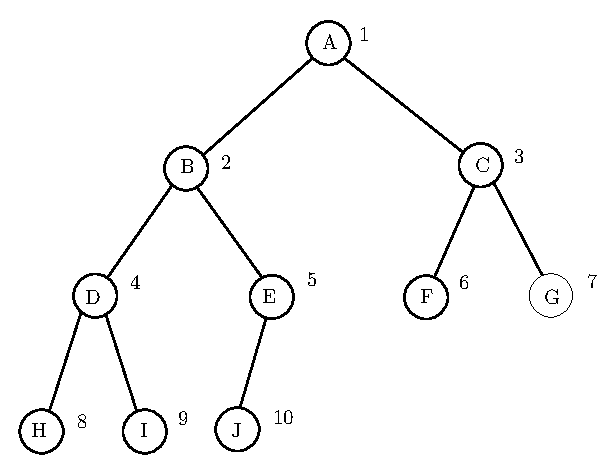
\includegraphics[width=80mm]{figs/tree-figTop.eps}}
\centerline{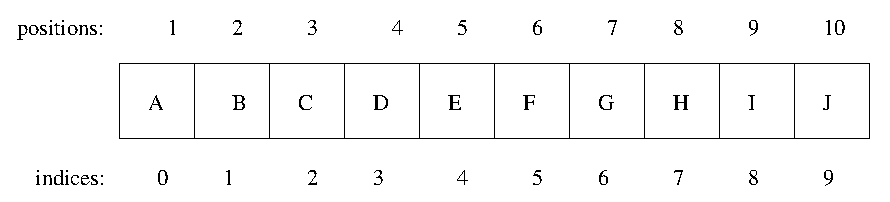
\includegraphics[width=80mm]{figs/tree-figBottom.eps}}
\caption{Complete binary tree and its array representation.}
\label{tree-fig} 
\end{figure}

A level-order traversal of a complete binary tree is easily stored
in a linear array as shown in Figure~\ref{tree-fig}. In this book 
we mostly use indices $0$ to $n-1$ for the array positions $1$ to $n$ 
in order to match popular programming languages such as Java, C, or C++. 
But the array representation of a binary tree is 
described more conveniently when both
the node numbers and the array positions are changing
from $1$ to $n$. Therefore, when a position $p$ in an array $a$
is mentioned below, we bear in mind 
an array element $a[i]$ with the index $i=p-1$.

The node in position $p$ has its parent node, left child, and right
child in positions $\lfloor p/2 \rfloor$, $2p$, and $2p + 1$,
respectively. The leaves have no children so that for each leaf node
$q$, the child position $2q$ exceeds the number of nodes $n$ in the
tree: $2q > n$.

\begin{Example}
In Figure~\ref{tree-fig},
the node in position $p=1$ is the root with no parent node. 
The nodes in positions from 6 to 10
are the leaves. The root has its
left child in position $2$ and its right child in position 
$3$. The nodes in positions $2$ and $3$ 
have their left child in position
$4$ and $6$ and their right child in position $5$ and $7$, respectively. 
The node in position $4$
has a left child in position $8$ and a right child in position
$9$, and the node $5$ has only a left child, in position $10$. 
\end{Example}

\begin{Definition}
A (maximum) \defnfont{heap} is a complete binary tree
having a key associated with each node,
the key of each parent node being greater than or
equal to the keys of its child nodes. 
\end{Definition} 

The heap order provides easy access to the maximum key  
associated with the root.

\begin{Example}
Figure~\ref{heap-fig} illustrates a maximum heap. Of
course, we could just as easily have a minimum heap  where
the key of the parent node is less than or equal to the keys
of its child nodes. Then the minimum key is associated with
the root. 
\end{Example}

\begin{figure}[htbp]
\begin{center}
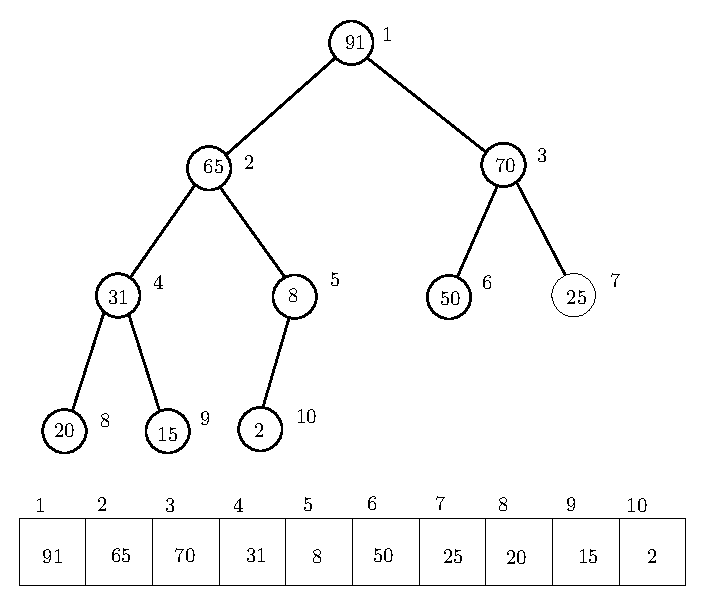
\includegraphics[width=80mm]{figs/heapmjd2ipe.eps}
\caption{\label{heap-fig} Maximum heap and its array representation.}
\end{center}
\end{figure}

The \defnfont{heapsort} algorithm now works as follows. Given an input list, 
build a heap by successively inserting the elements. Then delete the maximum 
repeatedly (arranging the elements in the output list in reverse order of 
deletion) until the heap is empty. Clearly, this is a variant of selection 
sort that uses a different data structure.

\subsection*{Analysis of heapsort}

Heapsort is clearly correct for the same reason as selection sort. To analyse its
performance, we need to analyse the running time of the insertion and deletion 
operations.

\begin{Lemma}\label{lem:tree:height}
The height of a complete binary tree with $n$ nodes
is at most $\lfloor \lg n \rfloor$.
\end{Lemma}

\begin{proof} Depending on the number of nodes at the bottom level,
a complete tree of height $h$ contains between $2^{h}$ and
$2^{h+1}-1$ nodes, so that \(2^{h} \le n < 2^{h+1}\),
or \(h \le \lg n < h+1\). \end{proof}


\begin{Lemma} 
Insertion of a new node into a heap takes logarithmic time. 
\end{Lemma}

\begin{proof}
To add one more node to a heap of \(n\) elements, a new,
\((n+1)\)-st, leaf position has to be created. The new node with 
its associated key is placed first in this leaf.  
If the inserted key preserves the heap order, the insertion is
completed. Otherwise, the new key has to swap with
its parent, and this process of \defnfont{bubbling up}, 
(or \emph{percolating up}) the key is repeated toward the root until the heap 
order is restored. Therefore, there are at most $h$ swaps where $h$ is the heap 
height, so that the running time is $O(\log n)$.
\end{proof}

\begin{Example}
To insert an 11th element, $75$, into the heap
in Figure~\ref{heap-fig} takes three steps.
\begin{itemize}
\item Position 11 to initially place the new key, $75$, is created.
\item The new key is swapped with its parent key, $8$, in
position $5 = \lfloor 11/2 \rfloor$ to restore the heap order.
\item The same type of swap is repeated for the parent key, $65$, 
in position $2 = \lfloor 5/2 \rfloor$. Because the heap order condition is now 
satisfied, the process terminates.
\end{itemize}

\begin{table}[htb!]
\caption{Inserting a new node with the key 75 in the heap 
in Figure~\ref{heap-fig}.}\label{t:insert:heap}
\centerline{
\begin{tabular}{|l|c|c|c|c|c|c|c|c|c|c|c|} \hline
\textbf{Position} & 1 & 2 & 3 & 4 & 5 & 6 & 7 & 8 & 9 & 10 & 11 \\ \hline 
\textbf{Index}   & 0 & 1 & 2 & 3 & 4 & 5 & 6 & 7 & 8 & 9 & 10 \\ \hline
Array at step 1 & 91 & 65 & 70 & 31 & 8 & 50 & 25 & 20 & 15 & 2 & \textbf{75} 
\\ %\hline
Array at step 2 & 91 & 65 & 70 & 31 & \textbf{75} & 50 & 25 & 20 & 15 & 2 & 
\emph{8} 
\\ %\hline
Array at step 3 & 91 & \textbf{75} & 70 & 31 & \emph{65} & 50 & 25 & 20 & 15 & 2 
& 8 
\\ \hline
\end{tabular}}
\end{table}

This is shown in Table~\ref{t:insert:heap}. The elements moved to
restore the heap order are italicized.

\end{Example}


\begin{Lemma} \label{lem:heap-delete}
Deletion of the maximum key from a heap takes logarithmic time in the worst case.
\end{Lemma}

\begin{proof}
The maximum key occupies the tree's root, that is, position 1 of the array.
The deletion reduces the heap size by 1 so that its last leaf node has to be 
eliminated. The key associated with this leaf replaces the deleted
key in the root and then is \defnfont{percolated down} the tree. 
First, the new root key is compared to each child and swapped with the larger 
child if at least one child is greater than the parent. This process is 
repeated until the order is restored. Therefore, there are $h$ moves in the 
worst case where $h$ is the heap height, and the running time is $O(\log n)$. 
\end{proof}

Because we percolate down the previous leaf key, the process usually
terminates at or near the leaves. 

%\newpage

\begin{Example}
To delete the maximum key, $91$, from the heap in Figure~\ref{heap-fig}, takes 
three steps, as follows.

\begin{itemize}
\item Key $2$ from the eliminated position 10 is placed at the root.
\item The new root key is compared to its children $65$ and $70$ in positions
 $2 = 2 \cdot 1 $  and $3 = 2 \cdot 1 + 1$, respectively. To restore 
the heap order, it is swapped with its larger child, $70$.
\item The same swap is repeated for the children $50$ and $25$ in 
positions $6 = 2 \cdot 3$ and $7 = 2 \cdot 3 + 1$. Because the heap order 
is now correct, the process terminates.
\end{itemize}

\begin{table}[htb!]
\caption{\label{t:delete:heap}
Deletion of the maximum key from the heap in Figure~\ref{heap-fig}.}
\centerline{
\begin{tabular}{|l|c|c|c|c|c|c|c|c|c|} \hline
\textbf{Position} & 1 & 2 & 3 & 4 & 5 & 6 & 7 & 8 & 9  \\ \hline
\textbf{Index}   & 0 & 1 & 2 & 3 & 4 & 5 & 6 & 7 & 8  \\ \hline
Array at step 1 & \textbf{ 2} & 65 & 70       & 31 & 8 & 50 & 25 & 20 & 15 
\\ %\hline
Array at step 2 & \emph{70} & 65 & \textbf{ 2} & 31 & 8 & 50 & 25 & 20 & 15  
\\ %\hline
Array at step 3 & \emph{70} & 65 & \emph{50} & 31 & 8 & \textbf{2} & 25 & 20 & 15 
\\ \hline
\end{tabular}}
\end{table}

See also Table~\ref{t:delete:heap}.
The leaf key replacing the root key is boldfaced, and the moves to restore the 
heap are italicized.

\end{Example}

\begin{Lemma}
Heapsort runs in time in $\Theta(n \log n)$ in the best, worst, and average case.
\end{Lemma}
\begin{proof}
The heap can be constructed in time $O(n \log n)$ (in fact it can be done more 
quickly as seen in Lemma~\ref{lem:quickheap} 
but this does not affect the result). Heapsort then repeats $n$ times the 
deletion of the maximum key and restoration of the heap property. 
In the best, worst,  and average case, each restoration is logarithmic, so the
 total time is $\log(n)+\log(n-1)+...+\log(1) = \log n!$ which is 
$\Theta(n \log n)$.
\end{proof}

\subsection*{Implementation of heapsort} 

There are several improvements that can be made to the basic idea above. First, 
the heap construction phase can be simplified. There is no need to maintain the 
heap property as we add each element, since we only require the heap property
once the heap is fully built. A nice recursive approach is shown below. Second, 
 we can eliminate the recursion. Third, everything can be done 
in-place starting with an input array. 

We consider each of these in turn.

A heap can be considered as a recursive structure
of the form \textsf{left subheap} $\leftarrow$ \textsf{root} $\rightarrow$
\textsf{right subheap}, built by a recursive ``heapifying''
process. The latter assumes that the heap order exists everywhere
except at the root and percolates the root down to restore the total
heap order. Then it is recursively applied to the left and right
subheaps. 

\begin{Lemma}
A complete binary tree satisfies the heap property if and only if the maximum 
key is at the root, and the left and right subtrees of the root also satisfy 
the heap property with respect to the same total order.
\end{Lemma}
\begin{proof}
Suppose that $T$ is a complete binary tree that satisfies the heap condition. 
Then the maximum key is at the root. The left and right subtrees at the root 
are also complete binary trees, and they inherit the heap property from $T$. 

Conversely, suppose that $T$ is a complete binary tree with the maximum at the
root and such that the left and right subtrees are themselves heaps. 
Then the value at the root is at least as great as that of the keys of the 
children of the root. For each other node of $T$, the same property holds by our
hypotheses. Thus the heap property holds for all nodes in the tree.
\end{proof}

For example, in Figure~\ref{heap-fig} we can see this fact clearly.
		
\begin{Lemma}\label{lem:quickheap}
A heap can be constructed from a list of size $n$ in $\Theta(n)$ time.
\end{Lemma}
\begin{proof}
Let $T(h)$ denote the worst-case time to build a heap of height at most $h$. 
To construct the heap, each of the two subtrees attached to the root are first 
transformed into  heaps of height at most $h-1$ (the left subtree is always of
height $h-1$, whereas the right subtree could be of lesser height, $h-2$). 
Then in the worst case the root percolates down the tree
for a distance of at most $h$ steps that takes time $O(h)$. 
Thus heap construction is asymptotically described by the
recurrence similar to Example~\ref{ex:exp:recurrence}, 
\(
T(h) = 2T(h-1) + ch
\) 
and so $T(h)$ is $O(2^{h})$. Because a heap of size $n$ is of height  
$h = \lfloor \lg n \rfloor$, we have $2^{h} \le n$ and thus 
\(T(h)\) is $O(n)$. But since every element of the input must be inspected, we 
clearly have a lower bound of $\Omega(n)$, which yields the result.
\end{proof}

Now we observe that the recursion above can be eliminated. The key at each position 
$p$ percolates down only after all its descendants have been already processed 
by the same percolate-down procedure.  Therefore, if this procedure is applied to
the nodes in reverse level order, the recursion becomes unnecessary. In
this case, when the node $p$ has to be processed, all its descendants
have been already processed. Because leaves need not percolate down,
a non-recursive heapifying process by percolating nodes down can start
at the non-leaf node with the highest number. This leads to an extremely simple 
algorithm for converting an array into a heap (see the first \textbf{for} loop 
in Figure~\ref{heapsort}).
    
Figure~\ref{heapsort} presents the basic pseudocode for heapsort (for details 
of the procedure $\algfont{percolateDown}$, see the Java code in 
Section~\ref{sec:app:order}). After each deletion, the heap size decreases by 1, 
and the emptied last
array position is used to place the just deleted maximum element. After
the last deletion the array contains the keys in ascending sorted
order. To get them in descending order, we have to build a minimum heap 
instead of the above maximum heap.

The first for-loop converts an input array $a$
into a heap by percolating elements down. The
second for-loop swaps each current maximum
element to be deleted with the current last position
excluded from the heap and restores the heap by percolating
each new key from the root down.

\begin{figure}[htb!]
\centerline{
\begin{minipage}{150mm}
\Algorithm{heapSort}{array $a[0..n-1]$}
{the sorted array $a$}
{ 
\>\textbf{for} $i \leftarrow \lfloor n/2 \rfloor - 1$
                 \textbf{while} $i \ge 0$
                 \textbf{step} $i\leftarrow i-1$ \textbf{do}\\
\> $\algfont{percolateDown}(a, i, n$ )
                 \hspace{5mm}\AlgCmt{build a heap}\\
\>\textbf{end for}\\
\>\textbf{for} $i \leftarrow  n - 1$
                 \textbf{while} $i \ge 1$
                 \textbf{step} $i\leftarrow i-1$ \textbf{do}\\
\>\>\algfont{swap}$( a[0] , a[i] )$
                 \hspace{22mm}\AlgCmt{delete the maximum}\\
\>\>$\algfont{percolateDown}(a, 0, i$ )
                 \hspace{8mm}\AlgCmt{restore the heap}\\
\>\textbf{end for}\\
}
\end{minipage}}
\caption{\label{heapsort} Heapsort.}
\end{figure} 

\begin{Example}
Table~\ref{heapsort-example} presents 
successive steps of heapsort on
the input array \(a=[70, 65, 50, 20, 2, 91, 25, 31, 15, 8]\). 
In the table, the keys moved are italicized and the 
items sorted are boldfaced.

\begin{table}[htbp]
\caption{\label{heapsort-example} Successive steps of heapsort.}
\begin{tabular}{|l|c|c|c|c|c|c|c|c|c|c|} \hline
\textbf{Position}      & 1 & 2 & 3 & 4 & 5 & 6 & 7 & 8 & 9 & 10  \\ %\hline 
\textbf{Index}         & 0 & 1 & 2 & 3 & 4 & 5 & 6 & 7 & 8 & 9 \\ \hline
Initial array & 70 & 65 & 50 & 20 & 2 & 91 & 25 & 31 & 15 & 8 
\\ %\hline 
Building max heap & 70 & 65 & 50 & 20 & \textit{8} & 91 & 25 & 31 & 15 & \textit{2} 
\\ %\cline{2-11}  
                  & 70 & 65 & 50 & \textit{31} & 8 & 91 & 25 & \textit{20} & 15 & 2  
\\ %\cline{2-11}  
                  & 70 & 65 & \textit{91} & 31 & 8 & \textit{50} & 25 & 20 & 15 & 2  
\\ %\cline{2-11}  
                  & 70 & \textit{65} & 91 & 31 & 8 & 50 & 25 & 20 & 15 & 2  
\\ %\cline{2-11}  
                  & \textit{91} & 65 & \textit{70} & 31 & 8 & 50 & 25 & 20 & 15 & 2  
\\ \hline 
Max heap          & 91 & 65 & 70 & 31 & 8  & 50 & 25 & 20 & 15 & 2 
\\ \hline 
Deleting max 1& \emph{2} & 65 & 70 & 31 & 8 & 50 & 25 & 20 & 15 & \textbf{91} 
\\ %\hline 
Restoring heap 1-9& \emph{70} & 65 & \emph{50} & 31 & 8 & \emph{2} & 25 & 20 & 15 & \textbf{91} 
\\ \hline 
Deleting max 2& \emph{15} & 65 & 50 & 31 & 8 & 2 & 25 & 20 & \textbf{70} & \textbf{91} 
\\ %\hline
Restoring heap 1-8& \emph{65} & \emph{31}  & 50 & \emph{20} & 8 & 2 & 25 & \emph{15} & \textbf{70} & \textbf{91} 
\\ \hline 
Deleting max 3& \emph{15} & 31 & 50 & 20 & 8 & 2 & 25 & \textbf{65} & \textbf{70} & \textbf{91} 
\\ %\hline
Restoring heap 1-7& \emph{50} & 31  & \emph{25} & 20 & 8 & 2 & \emph{15} 
& \textbf{65} & \textbf{70} & \textbf{91} 
\\ \hline 
Deleting max 4& \emph{15} & 31 & 25 & 20 & 8 & 2 & \textbf{50} & 
\textbf{65} & \textbf{70} & \textbf{91} 
\\ %\hline
Restoring heap 1-6& \emph{31} & \emph{20}  & 25 & \emph{15} & 8 & 2 & 
\textbf{50} 
& \textbf{65} & \textbf{70} & \textbf{91} 
\\ \hline 
Deleting max 5& \emph{2} & 20 & 25 & 15 & 8 
& \textbf{31} & \textbf{50} & \textbf{65} & \textbf{70} & \textbf{91} 
\\ %\hline
Restoring heap 1-5& \emph{25} & 20  & \emph{2} & 15 & 8 & \textbf{31} & 
\textbf{50} 
& \textbf{65} & \textbf{70} & \textbf{91} 
\\ \hline 
Deleting max 6& \emph{8} & 20 & 2 & 15 & \textbf{25} 
& \textbf{31} & \textbf{50} & \textbf{65} & \textbf{70} & \textbf{91} 
\\ %\hline
Restoring heap 1-4& \emph{20} & \emph{15}  & 2 & \emph{8} & \textbf{25} & 
\textbf{31} & \textbf{50} 
& \textbf{65} & \textbf{70} & \textbf{91} 
\\ \hline
Deleting max 7& \emph{8} & 15 & 2 & \textbf{20} & \textbf{25} 
& \textbf{31} & \textbf{50} & \textbf{65} & \textbf{70} & \textbf{91} 
\\ %\hline
Restoring heap 1-3& \emph{15} & \emph{8}  & 2 & \textbf{20} & \textbf{25} & 
\textbf{31} & \textbf{50} 
& \textbf{65} & \textbf{70} & \textbf{91} 
\\ \hline
Deleting max 8& \emph{2} & 8 & \textbf{15} & \textbf{20} & \textbf{25} 
& \textbf{31} & \textbf{50} & \textbf{65} & \textbf{70} & \textbf{91} 
\\ %\hline
Restoring heap 1-2& \emph{8} & \emph{2}  & \textbf{15} & \textbf{20} & 
\textbf{25} & \textbf{31} & \textbf{50} 
& \textbf{65} & \textbf{70} & \textbf{91} 
\\ \hline 
Deleting max 9& \emph{2} & \textbf{8} & \textbf{15} & \textbf{20} & 
\textbf{25} 
& \textbf{31} & \textbf{50} & \textbf{65} & \textbf{70} & \textbf{91} 
\\ \hline 
\end{tabular}
\end{table}
\end{Example}


\subsubsection*{Priority-queue sort}

A heap is a particular implementation of the \emph{priority queue} ADT (see 
Section~\ref{sec:app:adt-informal}). There are many
other such implementations. From an abstract point of view, heapsort simply 
builds a priority queue by inserting all the elements of the list to be sorted, then 
deletes the highest priority element repeatedly. Any priority queue 
implementation can be used to sort in the same way. 

For example, a very simple implementation of a priority queue is via an unsorted list.
In this case, building the queue is trivial, and the sorting algorithm is exactly
selection sort. Another simple implementation is via a sorted list. In this case,
the algorithm is just insertion sort (we don't really need to delete the elements
since the resulting list after building the priority queue is the output we are seeking). 

There are many more sophisticated implementations of priority queues. They are 
useful not only for sorting, but for several important graph algorithms covered 
in this book, and also for applications such as discrete event simulation. There
is still active research on finding better priority queue implementations.

Given that we can build a priority queue (such as a heap) in linear time, it is 
natural to ask whether we could implement a priority queue in such a way that 
the successive deletions can be done in better than $O(n\log n)$ time, thus 
yielding a sorting algorithm that is asymptotically faster in the worst case 
than any we have yet seen. Perhaps surprisingly, the answer is no for 
comparison-based algorithms, as we see in the next section.

\subsection*{Exercises}

\begin{Exercise}\label{exr:insert:heap}
Insert a 12th element, 85, into the final heap in Table~\ref{t:insert:heap}.
\end{Exercise}

%\begin{Exercise}\label{ex:min-heap}
%Use the same keys as in Figure~\ref{heap-fig} to exemplify a minimum heap. 
%\end{Exercise}

\begin{Exercise}\label{exr:delete:heap}
Delete the maximum key from the final heap in Table~\ref{t:delete:heap}
and restore the heap order.
\end{Exercise}

\begin{Exercise}\label{exr:heap:build}
Convert the array \([10,20,30,40,50,60,70,80,90]\) into a heap 
using the algorithm in Lemma~\ref{lem:quickheap}.
\end{Exercise}

\begin{Exercise}\label{exr:hsort:apply} 
Present in the same manner the successive steps of heapsort on
the already sorted input array 
\(a=[2, 8, 15, 20, 25, 31, 50, 65, 70, 91]\).
\end{Exercise}

\begin{Exercise}\label{exr:hsort:stable}
Determine whether heapsort is stable and compare it to insertion sort,
mergesort, and quicksort regarding this property. 
\end{Exercise}

\begin{Exercise}\label{exr:heapsort:sorted:already}
Determine whether the running time of heapsort on an already sorted array of 
size \(n\) differs significantly from the average-case running time.
\end{Exercise}

%\begin{Exercise}\label{exr:heapsort-extreme}
%Find lists of size $8$, 
%containing the integers $1, \dots, 8$ exactly once, that force heapsort to do the 
%maximum (minimum) number of comparisons.
%\end{Exercise}

\section{Data selection}\label{sec:qselect}

Data selection is closely related to data sorting. The latter arranges
an array in order whereas the former has to find only the $k$th smallest item 
(the item of \defnfont{rank} \(k\), also known as the 
$k$th \defnfont{order statistic}). We have seen (selection sort and heapsort) 
that if we can select, then we can sort. The converse is true too: 
given a list of $n$ items, we can sort it and then select the desired order 
statistic easily. The obvious question is: can we perform selection without sorting, 
and asymptotically faster?

If for example $k=1$ or $k=n$, then the answer is obviously yes 
(Exercise~\ref{exr:selectmax}). However, if we require the median 
($k=\lceil n/2 \rceil$) the answer is not at all obvious. For example, building 
a heap and repeatedly extracting the minimum would take time in 
$\Omega(n\log n)$, which is no better than sorting the entire list.

A variation of quicksort works well on this problem, \emph{in the average case for random 
data}. However it has all the drawbacks of quicksort, and in the worst case its 
performance degenerates badly.

The idea of \defnfont{quickselect} is that after the partitioning stage of quicksort, 
we know which of the two parts of the partition holds the element we are seeking, 
and so we can eliminate one recursive call. In other words, it proceeds as follows.
\begin{itemize}
\item  If the size of the list is 0, return ``not found"; if the size is 1, 
return the element of that list. Otherwise:
\item Choose one of the items in the list as a pivot. 
\item Partition the remaining items into two disjoint sublists: 
reorder the list by placing all items greater than the pivot to follow it,
 and all elements less than the pivot to precede it. Let $j$ be the index of the 
 pivot after partitioning.
\item If $k < j$, then return the result of quickselect on the ``head" sublist; 
otherwise if $k = j$, return the element $p$; otherwise return the result of 
quickselect on the ``tail" sublist.
\end{itemize}

%\begin{Example} 
%\label{ex:quickselect}
%\end{Example}

\subsection*{Analysis of quickselect}

Correctness of quickselect is established just as for quicksort 
(see Exercise~\ref{exr:quickselect-correctness}). In the worst case, the running
time can be quadratic; for example, if the input list is already sorted and we 
use the naive pivot selection rule, then to find the maximum element takes 
quadratic time. 

\begin{Theorem}\label{t:quickselect-average} 
The average-case time complexity of quickselect is $\Theta(n)$.  
\end{Theorem}

\begin{proof}
Let $T(n)$ denote the average time to select the $k$-th smallest element among 
$n$ elements, for fixed $k$ where the average is taken over all possible input
sequences. Partitioning uses no more than $cn$ operations and forms two 
subarrays, of size $i$ and $n-1-i$, respectively, where \(0 \leq i < n\).

As in quicksort, the final pivot position in the sorted
array has equal probability, \(\frac{1}{n}\), of taking each value of $i$.
Then \(T(n)\) averages the average running time for all the above
pairs of the subarrays over all possible  sizes. Because only one subarray from 
each pair is recursively chosen, the average running time for the pair
of size $i$ and $n-1-i$ is \((T(i)+T(n-1-i))/2\) so that
\begin{eqnarray*}
T(n) 
= \frac{1}{2n} \sum\limits_{i=0}^{n-1}(T(i)+T(n-1-i)) + cn 
= \frac{1}{n} \sum\limits_{i=0}^{n-1}T(i)  + cn
\end{eqnarray*}
As for quicksort, the above recurrence can be rewritten as
\(
n T(n)  = \sum_{i=0}^{n-1}T(i) + cn^{2}
\) and subtracting the analogous equation
 $(n-1)T(n-1) = \sum_{i=0}^{n-2}T(i) + c \cdot (n-1)^{2}$ and rearranging,
we are eventually led to the familiar recurrence
\(
T(n) = T(n-1) + c
\) and can see that $T(n)$ is $\Theta(n)$.
\end{proof}

\subsection*{Implementation of quickselect}

The only change from quicksort is that instead of making two recursive calls on the
left and right subarrays determined by the pivot, quickselect chooses just one of 
these subarrays.

\begin{figure}[htb!]
\hspace*{.5in}\begin{minipage}{5in}
\Algorithm{quickSelect}
{
\begin{minipage}[t]{5in}
array $a[0..n]$; array indices $l, r$; integer $k$\\
\AlgCmt{finds $k$th smallest element in the subarray $a[l..r]$}
\end{minipage}
}
{the element of $a[l..r]$ of rank $k$}
{
\> \textbf{if} $l \leq r$ \textbf{then} \\
\> \> $i \leftarrow \algfont{pivot}(a,l,r)$ \AlgCmt{return position of pivot element}\\
\> \> $j \leftarrow \algfont{partition}(a,l,r,i)$ \AlgCmt{return final position of pivot}\\
\> \> $q \leftarrow j - l + 1$ \AlgCmt{the rank of the pivot in $a[l..r]$}\\
\> \> \textbf{if} $k = q$ \textbf{then return} $a[j]$\\
\> \> \textbf{else if} $ k < q$ \textbf{then return} $\algfont{quickSelect}(a, l, j - 1, k)$ %\AlgCmt{try left subarray}
\\  
\> \> \textbf{else} \textbf{return} $\algfont{quickSelect}(a, j+1, r, k-q)$ 
%\AlgCmt{try right subarray} 
\\
\> \textbf{end if}\\
\> \textbf{else return} ``not found"\\
}
\end{minipage}
\caption{\label{fig:quickselect} Basic array-based quickselect.}
\end{figure} 


Figure~\ref{fig:quickselect} presents a basic array-based implementation. 
The algorithm processes a subarray
$a[l..r]$, where $0 \le l \le r \le n-1$, of an input array
$a$ of size $n$, assuming that the desired rank $k$ is
in the correct range. A search in the whole array is performed
with the input indices $l=0$ and $r=n-1$. The 
search fails only if $k$ is outside the correct range (including the case where 
the subarray is empty).
Section~\ref{sec:app:order} contains a Java implementation that uses median-of-three
pivoting.

\subsection*{Exercises}

\begin{Exercise}\label{exr:selectmax}
Give a simple nonrecursive algorithm to find the maximum of a list of $n$ 
elements. How many comparisons does it do in the worst case? 
Is this the best we can hope for?
\end{Exercise}

\begin{Exercise}\label{exr:quickselect-correctness}
Prove that quickselect is correct.
\end{Exercise}

\begin{Exercise}\label{exr:select:ranks}
To find \(p\) keys of fixed ranks, \(k_1 , \ldots, k_p \),
in an unordered array, we can either (i) run quickselect \(p\)
times or (ii) use quicksort once to order the array and simply
fetch the desired \(p\) keys. Find a condition (in terms of
\(p\) and \(n\)) when on the average the second variant is more
time-efficient (time to fetch array elements can be ignored). 
Which variant is better if $n$ is $1$ million and \(p=10\)?
\end{Exercise}

\begin{Exercise}\label{ex:heapselect}
Investigate ``heapselect" and its time complexity. Do the same for 
``mergeselect".
\end{Exercise}

\section{Lower complexity bound for sorting}
\label{sec:lower:bound}

All the above sorting methods have average and worst time complexity bounds in 
$\Omega(n \log n)$. One of most fundamental theorems in algorithm analysis 
shows that no comparison-based sorting algorithm can have a better asymptotic 
lower bound. The proof uses the idea of a $n$-element binary 
\defnfont{decision tree} representation of any sorting of $n$ items by pairwise comparisons. 

\begin{figure}[htb!]
\centerline{
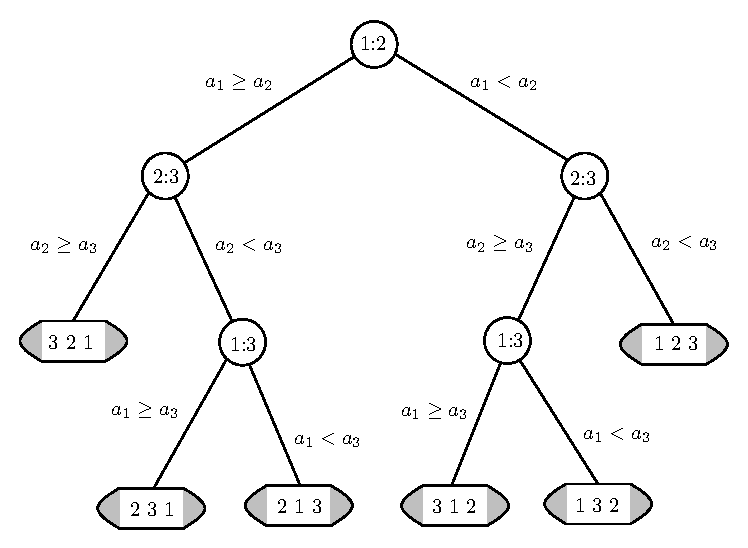
\includegraphics[width=80mm]{figs/tree123ipe.eps}
}
\caption{\label{tree123} Decision tree for $n=3$.}
\end{figure}

\begin{Example} A decision tree for three ($n=3$)
elements $a_1, a_2, a_3$ is shown in Figure~\ref{tree123}. 
Each internal tree node represents a pairwise comparison and decision made at a
particular step of sorting (in Figure~\ref{tree123}, $i:j$ denotes 
the comparison between the elements $a[i]$ and $a[j]$). 
Two downward arcs from the node indicate two possible
results of the comparison: $a[i] \geq a[j]$ or $a[i] < a[j]$. 
Leaves represent the sorted lists. In Figure~\ref{tree123}, each triple
$ijk$ denotes the sorted list $(a_i,a_j,a_k)$ obtained from
the initial list $(a_1 ,a_2 , a_3)$. For instance, \(123\),
\(213\), or \(321\) mean that the final list
is $(a_1 ,a_2 , a_3)$, $(a_2, a_1, a_3)$, or 
$(a_3 , a_2, a_1)$, respectively. 
Because any of the $n!$ permutations of $n$ arbitrary items 
$a_1, a_2, \ldots, a_n$ may be obtained as the result of 
the sort, the decision tree must have at least $n!$ leaves.
\end{Example}

The path length from the root to a leaf in the decision tree is equal to the 
number of comparisons  to be performed in order to  obtain the sorted array at 
the leaf. Therefore, the longest path (the height of the tree) equals
the number of comparisons in the worst case. For example, $3$ elements 
can be sorted with no more than $3$ comparisons because the height of the 
$3$-element tree in Figure~\ref{tree123} is equal to $3$. 

\begin{Theorem} \label{t:worst}
Every comparison-based sorting algorithm takes $\Omega(n\log n)$ time in the 
worst case.
\end{Theorem}

\begin{proof} 
We first claim that each binary tree of height $h$ has at most $2^{h}$ leaves. 
Once this claim is established, we proceed as follows. The least value $h$ such 
that $2^{h} \ge n!$ has the lower bound $h \ge \lg (n!)$ which is in
$\Omega(n \log n )$ (the asymptotic result follows from 
Section~\ref{sec:app:sum:series}). This will prove the theorem.

To prove the above claim about tree height, we use mathematical induction on 
$h$. A tree of height $0$ has obviously at most $2^{0}$ leaves. Now suppose 
that $h\geq 1$ and that each tree of height $h-1$ has at most $2^{h-1}$ 
leaves. The root of a decision tree of  height $h$ is linked to two subtrees, 
being each at most of height $h-1$. By the induction hypothesis, each 
subtree has at most $2^{h-1}$ leaves. The number of leaves in the whole decision
tree is equal to the total number of leaves in its subtrees, that is,
at most $2^{h-1}+2^{h-1}=2^{h}$.
\end{proof}

This result shows that heapsort and mergesort have asymptotically optimal 
worst-case time complexity for comparison-based sorting.

As for average-case complexity, one can also prove the following
theorem by using the decision tree idea. Since we are now at the end of
our introductory analysis of sorting, we omit the proof and refer the
reader to the exercises, and to more advanced books.

\begin{Theorem}\label{t:average}
Every comparison-based sorting algorithm takes $\Omega(n \log n)$ time
in the average case. 
\end{Theorem}

\begin{proof}
Try to prove this yourself (see Exercise~\ref{ex:prove-lower-bound}).
\end{proof}
\subsection*{Exercises}

\begin{Exercise} \label{ex:prove-lower-bound} 
Prove Theorem~\ref{t:average}. The following hints may be useful. First
show that the sum of all depths of leaves in a binary decision tree with $k$
leaves is at least $k \lg k$. Do this by  induction on $k$, using the
recursive structure of these trees. Then apply the above inequality 
with $k=n!$.
\end{Exercise}

\begin{Exercise}
\label{ex:radix}
Consider the following sorting method (often called \defnfont{counting sort}) 
applied to an array $a[n]$ all of whose entries are integers in the range 
$1..1000$. Introduce a new array $t[1000]$ all of whose entries are initially 
zero. Scan through the array $a[n]$ and each time an integer $i$ is found, 
increment the counter $t[i-1]$ by $1$. Once this is complete, loop through 
$0 \leq i\leq 999$ and print out $t[i]$ copies of integer $i+1$ at each step.

What is the worst-case time complexity of this algorithm? How do we reconcile 
this with Theorem~\ref{t:worst}?
\end{Exercise}


\section{Notes}
It was once said that sorting consumes 25\% of all CPU time worldwide. Whatever
the true proportion today, sorting clearly remains a fundamental problem to be 
solved in a wide variety of applications.

Given the rise of object-oriented programming languages,  comparison-based 
sorting algorithms are perhaps even more important than in the past. In practice
the time taken to perform a basic comparison operation is often much more than that 
taken to swap two objects: this differs from the case of, say, 32-bit integers,
for which most analysis was done in the past. 

Shellsort was proposed by D. Shell in 1959, quicksort by C. A. R. Hoare in 1960,
mergesort in 1945 by J. von Neumann, and heapsort in 1964 by J. W. J. Williams. 
Insertion sort and the other quadratic algorithms are very much older.

At the time of writing, versions of mergesort are used in the standard libraries for
the languages Python, C++ and Java, and a hybrid of quicksort and heapsort is used
by C++.

We have not discussed whether there is an algorithm that will find the 
median (or any other given order statistic) in worst-case linear time.
For a long time this was unknown, but the answer was shown to be yes in 1973 by 
Blum, Floyd, Pratt, Rivest and Tarjan. The algorithm is covered in more 
advanced books and is fairly complicated. 




\chapter{Efficiency of  Searching}
\label{CH:EFF:SEARCH}

Searching in a large database is a fundamental computational
task. Usually the information is partitioned into \defnfont{records}
and each record has a \defnfont{key} to use in the search. Suppose  we have a 
data structure $D$ of records. The search problem is as follows: given a search 
key $k$, either return the record associated with $k$ in $D$ (a 
\defnfont{successful search}), or indicate that $k$ is not found, without 
altering $D$ (an \defnfont{unsuccessful search}). If $k$ occurs more than once,
return any occurrence. The purpose of the search is usually to access data in 
the record (not merely the key). Simple examples are  searching a phone 
directory or a dictionary.

In this chapter we discuss searching in a general data structure as above. The 
more specialized problem of searching for a pattern in a text string is covered 
%later in Section~\ref{sec:strmatch}.
in the printed version of this textbook.

\section{The problem of searching}
\label{sec:search}

The most general data structure that allows searching is called an 
\emph{associative array},  \emph{table} or \emph{dictionary}.

In the general case, a key and a value are linked by \emph{association}.
An \defnfont{associative array} or \defnfont{dictionary} is an abstract 
data type relating a disjoint set of keys to an arbitrary set of values. Keys of
entries of an associative array may not have any ordering relation and may be
of unknown range. There is no upper bound on the size of this structure,
so that it can maintain an arbitrary number of different pieces of
information simultaneously. The analogy with a conventional word
dictionary may be misleading, because the latter has a lexicographical
order while dictionary structures need not be ordered.

Another name for this data type is \defnfont{table}. 
It takes its name from program compilation where
 a symbol table is used to record variables of a program, together with their
type, address, value, etc. Symbol table operations are also
fundamental to database systems.

\begin{Definition} The \defnfont{table} ADT is a set of ordered pairs 
(table entries) of the form \((k,v)\) where \(k\) is an unique \emph{key} and 
\(v\) is a data \emph{value} associated with the key \(k\). Each key uniquely
identifies its entry, and table entries are distinguished by keys
because no two distinct entries have identical keys. 

Basic operations defined for this structure are: construct (initialize) an 
empty table, enumerate table entries, search for an entry, insert, delete, retrieve, and 
update table entries.
\end{Definition}

Abstractly, a table is a mapping (function) from keys to values. Given a 
search key \(k\), \defnfont{table search} has to find the table entry 
\((k,v)\) containing that key. The found entry may be retrieved, or removed 
(deleted) from the table, or its value, \(v\), may be updated. If the table
has no such entry, a new entry with key \(k\) may be  created and inserted in 
the table. Operations on a table also initialize a table to the 
empty one or indicate that an entry with the given key is absent. Insertions 
and deletions modify the mapping of keys onto values specified by
the table.

\begin{Example}
\label{exm:adt:airports} 
Table~\ref{tab:adt-tbl} 
presents a very popular (at least in textbooks on algorithms and data
structures)  table having three-letter identifiers
of airports as keys and associated data such as
airport locations, as values. Each identifier
has a unique integer
representation \(k = 26^2 c_0 + 26c_1 + c_2\) where the \(c_i\); 
\(i=0,1,2\), are ordinal numbers of 
letters in the English alphabet
(A corresponds to  0, B to 1, \ldots, Z to 25). For example, 
AKL corresponds to $26^2 \cdot 0 + 26\cdot 10 + 11 = 271$. In total, there are  
$26^3=17576$ possible different keys and entries.
\end{Example}

\begin{table}[htb!]
\caption{\label{tab:adt-tbl}
A map between airport codes and locations.}
\centerline{
\begin{tabular}{|lr|lll|}\hline
\multicolumn{2}{|c|}{\textbf{Key}} &
\multicolumn{3}{c|}{\textbf{Associated value} \(v\)} 
\\ \hline
Code& \(k\) & City & Country & State / Place \\ \hline
AKL & 271 & Auckland    & New Zealand &                \\
DCA &2080 & Washington  & USA         & District of Columbia (D.C.) \\
FRA &3822 & Frankfurt   & Germany     & Hesse \\
GLA &4342 & Glasgow     & UK          & Scotland \\
HKG &4998 & Hong Kong   & China       &                \\
LAX &7459 & Los Angeles & USA         & California \\
SDF &12251& Louisville  & USA         & Kentucky  \\
ORY &9930 & Paris       & France      &              \\ \hline
\end{tabular}}
\end{table}

As can be seen from this example, we may map the keys to integers.

We deal with both \defnfont{static} (where the database is fixed in 
advance and no insertions, deletions or updates are done) and \defnfont{dynamic} 
(where insertions, deletions or updates are allowed) implementations of the table
ADT.

In all our implementations of the table ADT, we may simplify the analysis as follows. 
We use lists and trees as our basic containers. We treat each query or update of 
a list element or tree node, or comparison of two of them, as an elementary operation. 
The following lemma summarizes some obvious relationships.

\begin{Lemma}\label{lem:ss-us}
Suppose that a table is built up from empty by successive insertions, and we 
then search for a key $k$ uniformly at random. 
Let $T_{ss}(k)$ (respectively $T_{us}(k)$) be the time to 
perform successful (respectively unsuccessful) search for $k$. Then
\begin{itemize}
\item the time taken to retrieve, delete, or update an element with key $k$ is at least 
$T_{ss}(k)$; 
\item the time taken to insert an element with key $k$ is at least $T_{us}(k)$;
\item $T_{ss}(k) \leq T_{us}(k)$.
\end{itemize}

%\newpage
In addition
\begin{itemize}
\item
the worst case value for $T_{ss}(k)$ equals the worst case value for $T_{us}(k)$;
\item the average value of $T_{ss}(k)$ equals one plus the average of the 
times for the unsuccessful searches undertaken while building the table.
\end{itemize}
\end{Lemma}
\begin{proof}
To insert a new element, we first try to find where it would be if it were contained 
in the data structure, and then perform a single insert operation into the container. 
To delete an element, we first find it, and then perform a delete operation on the 
container. Analogous statements hold for updating and retrieval.
Thus for a given state of the table formed by insertions from an empty table, 
the time for successful search for a given element is the time that it took for 
unsuccessful search for that element, as we built the table, plus one. This means that 
the time for unsuccessful search is always at least the time for successful search 
for a given element (the same in the worst case), and the average time for 
successful search for an element in a table is the average of all the times for 
unsuccessful searches plus one. 
\end{proof}

If the data structure used to implement a table arranges the records in a list, 
the efficiency of searching depends on whether the list is sorted. In the case 
of the telephone book, we quickly find  the desired phone number (data record) 
by name (key). But it is almost hopeless to search directly for a phone number 
unless we have a special reverse directory where the phone number serves as a 
key. We discuss unsorted lists in the Exercises below, and sorted lists in the 
next section.


\subsection*{Exercises}

\begin{Exercise} \label{exr:seq-search}

The \defnfont{sequential search} algorithm 
simply starts at the head of a list and examines 
elements in order until it finds the desired key or reaches the end of the list. 
An array-based version is shown in Figure~\ref{seq-search}.

\begin{figure}[htb!]
\hspace*{1.2in}\begin{minipage}{5in}
\Algorithm{sequentialSearch}
{array $a[0..n-1]$; key $k$}
{index $i$ such that $a[i] = k$, or indicator ``not found''} 
{
\> \textbf{for} \(i\) $\leftarrow$ 0 \textbf{while} \(i < n\) 
                 \textbf{step} $i \leftarrow i+1$ \textbf{do}\\
\> \>\textbf{if} $a[i] = k$ 
              \textbf{then} \textbf{return} $i$ \\
\> \textbf{end for}\\
\> \textbf{return} \textsf{not found}\\
}
\end{minipage}
\caption{\label{seq-search} A sequential search algorithm.}
\end{figure}

Show that both successful and unsuccessful sequential  search in a list of size 
$n$ have worst-case and average-case time complexity $\Theta(n)$. 
\end{Exercise}

\begin{Exercise} \label{exr:seq-search-sorted}
Show that sequential search is slightly more efficient for sorted lists than 
unsorted ones. What is the time complexity of successful and unsuccessful search?
\end{Exercise}

\section{Sorted lists and binary search}\label{sec:bin:search}

A sorted list implementation allows for much better search method
that uses the divide-and-conquer paradigm. The basic idea of 
\defnfont{binary search} is simple. 
Let $k$ be the desired key for which we want to search.
\begin{itemize}
\item If the list is empty, return ``not found". Otherwise:
\item Choose the key $a[m]$ of the middle element of the list. If $a[m]=k$, return its record; 
if $a[m] > k$, make a recursive call on the head sublist;  if $a[m]<k$, make a 
recursive call on the tail sublist.
\end{itemize}

\begin{Example}
\label{eg:binsearch}
Figure~\ref{bsear-ex} illustrates binary search for
the key $k=42$ in a list of size 16. At the
first iteration, the search key 42 is compared to the 
key $a[7]  = 53$ in the middle position
$m=\lfloor (0+15)/2 \rfloor = 7$. 

\begin{figure}[htb!]
\centerline{
\illustr{bsear-ex.ps}{100mm}}
\caption{\label{bsear-ex} Binary search for the key 42.}
\end{figure}

Because $42 < 53$, the
second iteration explores the first half of the list
with positions $0,\ldots,6$. The search key is compared
to the key $a[3] = 33$ in the middle position
$m=\lfloor (0+6)/2 \rfloor = 3$. Because $42 > 33$, the
third iteration explores the second half of the current
sublist with positions $4,\ldots,6$. The comparison
to the key $a[5] = 49$ in the middle
position $m=\lfloor (4+6)/2 \rfloor = 5$ reduces the
search range to a single key, $a[4] = 42$,
because now $l = r = m = 4$. 
Because the single entry is equal to the search key, the
algorithm returns the answer 4.
\end{Example}


\subsection{Analysis of sorted list-based tables}
\label{sec:binsearch}

Binary search is readily seen to be correct by induction on the size of the list
(Exercise~\ref{exr:binary-search-correct}). 

The performance of binary search on an array is much better than on a linked list
because of the constant time access to a given element.

\begin{Lemma}
Consider a sorted list implementation of the table ADT.

Using an array, both successful and unsuccessful search take time in 
$\Theta(\log n)$, in both the average and worst case, as do retrieval and 
updating. Insertion and deletion take time in $\Theta(n)$ in the worst and 
average case.

Using a linked list, all the above operations take time in $\Theta(n)$. 
\end{Lemma}

\begin{proof}
Unsuccessful binary search takes $\lceil \lg (n+1)\rceil$ comparisons in 
every case, which is $\Theta(\log n)$. By Lemma~\ref{lem:ss-us}, 
successful search also takes time in $\Theta(\log n)$ on average and in the 
worst case. Insertion and deletion in arrays takes $\Theta(n)$ time on average 
and in the worst case.

For linked lists, the searches take time in $\Theta(n)$ and the list insertion 
and deletion take constant time.
\end{proof}

Binary search performs a predetermined sequence of comparisons
depending on the data size $n$ and the search key $k$. This sequence
is better analysed when a sorted list is represented as a 
\defnfont{binary search tree}. For simplicity of presentation, we suppress 
the data records and make all the keys integers. Background information on trees
is found in Section~\ref{sec:app:trees}.

\begin{Definition}
A \defnfont{binary search tree} (BST) is a binary tree that
satisfies the following ordering relation:
for every node $\nu$ in the tree, the values of all the keys
in the left subtree are smaller than (or equal, if duplicates allowed) 
to the key in $\nu$ and the  values of all the keys in the right 
subtree are greater than the key in $\nu$.
\end{Definition}

In line with the ordering relation, all the keys can be placed in sorted
order by traversing the tree in the following way: recursively visit,
for each node, its left subtree, the node itself, then its right subtree
(this is the so-called \defnfont{inorder} traversal). The relation is
not very desirable for duplicate keys; for exact data duplicates, we
should have one key and attach to it the number of duplicates.

The element in the middle position, $m_{0}=\lfloor (n-1)/2\rfloor$, of a
sorted array is the root of the tree representation.  The lower subrange,
$[0,\ldots,m_{0}-1]$, and the upper subrange, $[m_{0}+1,\ldots,n-1]$,
of indices are related to the left and right arcs from the root.
The elements in their middle positions, $m_{\mathrm{left},1}=\lfloor
(m_{0}-1)/2 \rfloor$ and $m_{\mathrm{right},1}=\lfloor (n + m_{0})/2
\rfloor$, become the left and right child of the root, respectively. This process 
is repeated until all the array elements are
related to the nodes of the tree. The middle element of each subarray
is the left child if its key is less than the parent key or the right
child otherwise.

\begin{figure}[htb!]
\centerline{
\illustr{btree-ex.ps}{100mm}}
\caption{\label{btree-ex} Binary tree representation of
a sorted array.}
\end{figure}
\begin{Example}
Figure~\ref{btree-ex}
shows a binary search tree for the 16 sorted keys in
Figure~\ref{bsear-ex}.
The key $a[7] =53$ is the root of
the tree. The lower $[0..6]$ and the upper $[8..15]$
subranges of the search produce the two children of the root:
the left child $a[3] =33$ and the right child
$a[11] =81$. All other nodes are built similarly.
\end{Example}

The tree representation interprets binary search
as a pass through the tree from the root to a desired key.
If a leaf is reached but the key is not found, then the search
is unsuccessful. The number of comparisons to find a key 
is equal to the number of nodes along the unique path from the root to
the key (the depth of the node, plus one).

A static binary search always yields a tree that is well-balanced:
for each node in the tree, the left and right subtrees have height that differs 
by at most $1$. Thus all leaves are on at most two levels. This property is used 
to define AVL trees in Section~\ref{sec:balanced}.


\subsection{Implementation of binary search}

Algorithm \algfont{binarySearch} in Figure~\ref{bin-search} 
searches for key \(k\) in a sorted array $a$.

\begin{figure}[htb]
\hspace*{.7in}\begin{minipage}{5in}
\Algorithm{binarySearch}
{array $a[0..n-1]$; key $k$}
{index $i$ such that $a[i] = k$, or indicator ``not found''}
{
\> $l \leftarrow 0$; $r\leftarrow n-1$\\
\> \textbf{while} $l \le r$ \textbf{do}\\ 
\> \>$m\leftarrow\lfloor(l+r)/2\rfloor$\\
\> \>\textbf{if} $a[m] < k$
             \textbf{then} $l \leftarrow m+1$\\
\> \>\textbf{else} \textbf{if} $a[m] > k$ 
             \textbf{then} $r\leftarrow m-1$
             \textbf{else} \textbf{return} $m$\\
\> \>\textbf{end if}\\
\> \textbf{end while}\\
\> \textbf{return} \textsf{not found}\\
}
\end{minipage}
\caption{\label{bin-search} Binary search with three-way comparisons.}
\end{figure}

The search starts from the whole
array from $l=0$ to $r=n-1$. If \(l\) and \(r\) ever
cross, $l > r$, then the desired
key is absent, indicating an unsuccessful search. Otherwise,
the middle position of the odd range or rounded down
``almost middle'' position  of 
the even one, $m=\left\lfloor\frac{l+r}{2}\right\rfloor$,  is computed.
The search key, $k$, is compared to the key $a[m]$ in this position:

\begin{itemize}
 \item If $k = a[m]$,
then return the found position $m$.
 \item If $k < a[m]$, then the key may be
in the range $l$ to $m-1$ so that $r\leftarrow m-1$ at next step. 
 \item If $k > a[m]$, then it
may be in the range $m+1$ to $r$ so that $l\leftarrow m+1$ at next step. 
\end{itemize}

Binary search is slightly accelerated if the test for a successful
search is removed from the inner loop in Figure~\ref{bin-search} and the
search range is reduced by one in all cases. To determine whether
the key $k$ is present or absent, a single test is performed outside the
loop (see Figure~\ref{fast-bin-search}). If the search key $k$ is not
larger than the key $a[m]$ in the middle position $m$, then it may be in
the range from $l$ to $m$. The algorithm breaks the while-loop when the
range is 1, that is, $l = r$, and then tests whether there is a match.

\begin{figure}[htb!]
\hspace*{1.3in}\begin{minipage}{5in}
\Algorithm{binarySearch2}
{array $a[0..n-1]$; key $k$}
{index $i$ such that $a[i] = k$, or indicator ``not found''}
{
\> $l \leftarrow 0$; $r\leftarrow n-1$\\
\> \textbf{while} $l < r$ \textbf{do}\\ 
\> \>$m\leftarrow\lfloor(l + r)/2\rfloor$\\
\> \>\textbf{if} $a[m] < k$
               \textbf{then} $l\leftarrow m+1$\\
\> \>\textbf{else} $r \leftarrow m$\\
\> \textbf{end while}\\
\> \textbf{if} $a[l] = k$ \textbf{then} 
                \textbf{return} $l$ \\
\> \textbf{else} \textbf{return} \textsf{not found} \\
}
\end{minipage}
\caption{\label{fast-bin-search} Faster binary search with two-way
comparisons.}
\end{figure}

\subsection*{Exercises}

\begin{Exercise}
\label{ex:binsearch}
Perform a search for the key $41$ in the situation of 
Example~\ref{eg:binsearch}.
\end{Exercise}

\begin{Exercise}\label{exr:binsearch:comp}
How many comparisons will binary search make in the
worst case to find a key in a sorted array of size \(n=10^6\)?
\end{Exercise}

\begin{Exercise}\label{exr:binary-search-correct}
Prove that both given array implementations of binary search correctly find an 
element or report that it is absent.
\end{Exercise}

\begin{Exercise}\label{exr:interpol-search-bad}
If we have more information about a sorted list, \defnfont{interpolation search} 
can be (but is not always) much faster than binary search. It is the method 
used when searching a telephone 
book: to find a name starting with ``C" we open the book not in the middle, but 
closer to the beginning. 

To search for an element between position $l$ and $r$ with $l < r$, we choose 
\(\rho = \frac{ k - a[l]}{a[r] - a[l]}\)
and the next guess is  
\(
m = l + 
\left \lceil \rho (r - l) \right \rceil.
\)

Give an example of a sorted input array of $8$ distinct integers 
for which interpolation search performs no better than sequential search.
\end{Exercise}

\begin{Exercise}\label{exr:interpol:search}
Determine how many positions interpolation search will
examine to find the key \(85\) among the ten keys 
\((10,20,35,45,55,60,75,80,85,100)\).
\end{Exercise}

\section{Binary search trees}
\label{bin-search-tree}

In Section~\ref{sec:binsearch} we have already used a binary search
tree to specify sequences of comparisons and simplify the performance
analysis of binary search. Now we use a binary search tree not just as a mathematical 
object to aid our analysis, but as an explicit data structure that implements the 
table ADT. 

\begin{figure}[htb!]
\centerline{
\illustr{btree-e1.ps}{80mm}}
\caption{\label{btree-e1} Binary trees: only the leftmost tree is
a binary search tree.}
\end{figure}
\begin{Example}
In Figure~\ref{btree-e1}, two trees are not binary search trees 
because the key $2$ in the middle tree is
in the right subtree of the key $3$, 
and the keys $11$ and $12$ in the rightmost tree are
in the left subtree of the key $10$.
\end{Example}
Binary search trees implement efficiently the basic search, insert, and remove
operations of the table ADT. In addition a BST allows for more operations 
such as sorting records by their keys, finding the minimum key, etc (see Exercises).

Binary search trees are more complex than heaps. Only a root or 
leaves are added to or removed from a heap, whereas
any node of a binary search tree may be removed.

\begin{figure}[htbp]
\centerline{
\illustr{findinsr.ps}{70mm}}
\caption{\label{findinsr} Search and insertion in the binary search tree.}
\end{figure}

The search operation resembles usual binary search in that it starts 
at the root and moves either left or right along the tree, depending on 
the result of comparing the search key to the key in the node. 

\begin{Example}
\label{exm:find:a}
To find key $\textsf{8}$ in the leftmost tree in
Figure~\ref{btree-e1}, we
start at the root $10$ and go left because $\textsf{8} < 10$. This move
takes us to $3$, so we turn right (because $\textsf{8} > 3$) to $5$. Then we
go right again ($\textsf{8} > 5$) and encounter $8$. 
\end{Example}

\begin{Example}
\label{exm:find:b}
To find key $7$, we repeat the same path. But, when we are at node $8$, we 
cannot turn left because there is no such link. Hence, $7$ is not found. 
\end{Example}

Figure~\ref{findinsr} illustrates both Examples~\ref{exm:find:a} and
\ref{exm:find:b}. It shows that the node with key $7$ can be inserted
just at the point at which the unsuccessful search terminates.  

The removal operation is the most complex because removing a node may
disconnect the tree. Reattachment must retain the ordering condition but
should not needlessly increase the tree height. The standard method of removing 
a node is as follows.
\begin{itemize}
\item A leaf node is simply deleted. 
\item An internal node with only one child
is deleted after its child is linked to its parent node.
\item If the node has two children, then it should be swapped with the node 
having the smallest key in its right subtree. 
The latter node is easily found (see Exercise~\ref{exr:bst-min-max-med}). After 
swapping, the node can be removed as in the previous cases, since it is now in 
a position where it has at most one child. 
\end{itemize}

This approach appears asymmetric but various modifications do not really
improve it. The operation is illustrated in Figure~\ref{btr-dele}.

\begin{figure}[htb!]
\centerline{
\illustr{btr-dele.ps}{80mm}
}
\caption{\label{btr-dele} Removal of the node with key $10$ from
the binary search tree.}
\end{figure}

\subsection{Analysis of BST-based tables}

\begin{Lemma}
The search, retrieval, update, insert and remove operations in a BST 
all take time in $O(h)$ in the worst case, where $h$ is the height of the tree. 
\end{Lemma}
\begin{proof}
The running time of these operations is proportional to the 
number of nodes visited. For the find and insert operations, this equals 
$1$ plus the depth of the node, but for the remove operation it equals the 
depth of the node plus at most the height of the node. In each case this is 
$O(h)$. 
\end{proof}

For a well-balanced tree, all operations take logarithmic time. The problem is 
that insertions and deletions may destroy the balance, and in practice BSTs 
may be heavily unbalanced as in Figure~\ref{btr-bala}. So in the worst case the 
search time is linear, $\Theta(n)$, and we have an inferior form of sequential search 
(because of the extra overhead in creating the tree arcs).

Figure~\ref{btr-4b} presents all variants of inserting the four 
keys $1$, $2$, $3$, and $4$ into an empty binary search tree. Because only 
relative ordering is important, this corresponds to any four keys 
\((a[i]: i=1,\ldots,4)\) such that
\(
a[1] < a[2] < a[3] < a[4]
\).

\begin{figure}[htb!]
\centerline{
\illustr{btr-4a.ps}{120mm}}
\centerline{
\illustr{btr-4b.ps}{80mm}}
\caption{\label{btr-4b} Binary search trees obtained by
permutations of $1,2,3,4$.}
\end{figure}

There are in total $4!=24$ possible insertion orders given in
Figure~\ref{btr-4b}.
Some trees result from several different insertion sequences, and more balanced 
trees appear more frequently than unbalanced ones.


\begin{Definition}
The \defnfont{total internal path length}, 
\(S_\tau(n)\), of a binary tree $\tau$  is the sum of the 
depths of all its nodes. 
\end{Definition}

The average node depth, \(\frac{1}{n}S_{\tau}(n)\),
gives the average time complexity of a successful search in a
particular tree $\tau$. The average-case time complexity of searching
is obtained by averaging the total internal path lengths for all the trees of 
size \(n\), that is, for all possible \(n!\) insertion orders, assuming that 
these latter occur with equal probability, \(\frac{1}{n!}\). 


\begin{Lemma}\label{lem:bst:ave}
Suppose that a BST is created by $n$ random insertions starting from an empty tree.
Then the expected time for successful and unsuccessful search is 
$\Theta(\log n)$. The same is true for update, retrieval, insertion and deletion.
\end{Lemma}

\begin{proof}
Let $S(n)$ denote the average of $S_\tau$ over all insertion 
sequences, each sequence considered as equally likely. 
We need to prove that $S(n)$ is $\Theta(n \log n)$. 

It is obvious that $S(1)=0$. Furthermore, any $n$-node tree,
$n > 1$, contains a left subtree with $i$ nodes, a root at height $0$,
and a right subtree with $(n-i-1)$ nodes where $0 \le i \le n-1$,
each value of $i$ being by assumption equiprobable. 

For a fixed $i$, $S(i)$ is the average total internal path length in the
left subtree with respect to its own root and $S(n-i-1)$ is the
analogous total path length in the right subtree. The root of the tree
adds $1$ to the path length of each other node. Because there are
$n-1$ such nodes, the following recurrence holds:
\(S(n) = (n-1) + S(i) + S(n-i-1)\) for \(0 \le i \le n-1\).
After summing these recurrences for all $i=0,\ldots,n-1$ and averaging,
just the same recurrence as for the average-case 
quicksort analysis (see Lemma~\ref{lem:qsort:ave:comp}) is obtained:
\(
S(n) = (n-1) + \frac{2}{n} \sum_{i=0}^{n-1} S(i) 
\).
Therefore, the average total internal path length is $\Theta(n \log n)$. The 
expected depth of a node is therefore in $\Theta(\log n)$. This means that 
search, update, retrieval and insertion take time in $\Theta(\log n)$. The same 
result is true for deletion (this requires the result that the expected height 
of a random BST is $\Theta(\log n)$, which is harder to prove---see Notes).
\end{proof}

Thus in practice, for random input, all BST operations take time about 
$\Theta(\log n)$. However the worst-case linear time complexity, $\Theta(n)$, 
is totally unsuitable in many applications, and deletions can also destroy 
balance. 

We tried to eliminate the worst-case degradation of 
quicksort by choosing a pivot that performs well on random input data
and relying on the very low probability of the worst case. Fortunately, binary 
search trees allow for a special general technique, called \defnfont{balancing}, 
that guarantees that the worst cases simply cannot occur. Balancing 
restructures each tree after inserting new nodes in such a way as to prevent 
the tree height from growing too much. We discuss this more in 
Section~\ref{sec:balanced}.

\begin{figure}[htb!]
\centerline{
\illustr{btr-blns.ps}{60mm}}
\caption{\label{btr-blns} Binary search trees of height about $\log n$.}
\end{figure}

\begin{figure}[htb!]
\centerline{
\illustr{btr-bala.ps}{60mm}}
\caption{\label{btr-bala} Binary search trees of height about $n$.}
\end{figure}


\subsection{Implementation of BST}

A concrete implementation of a BST requires explicit links between nodes, each 
of which contains a data record, and is more complicated than the other 
implementations so far. A programming language that supports easy manipulation of
objects makes the coding easier. We do not present any (pseudo)code in this book.

\subsection*{Exercises}

\begin{Exercise}\label{exr:bst-min-max-med}
Show how to find the maximum (minimum) key in a binary search tree. What is the 
running time of your algorithm? How could you find the median, or an arbitrary 
order statistic?
\end{Exercise}

\begin{Exercise} \label{bst-dist}
Suppose that we insert the elements $1,2,3,4,5$ into an initially 
empty BST. If we do this in all 120 possible orders, which trees occur most often? 
Which tree shapes (in other words, ignore the keys) occur most often?
\end{Exercise}

\begin{Exercise} \label{exr:bst-extreme}

Suppose that we insert the elements $1,2,3,4$ in some order into an initially 
empty BST. Which insertion orders yield a tree of maximum height? Which yield a 
tree of minimum height?  
\end{Exercise}

\begin{Exercise}\label{exr:bst-sort}
Show how to output all records in ascending order of their keys, given a BST. 
What is the running time of your algorithm? 
\end{Exercise}

\section{Self-balancing binary and multiway search trees}
\label{sec:balanced}

Because balanced binary search trees are more complex than the standard
ones, the insertion and removal operations usually take
longer time on the average. But because of the resulting balanced structure,
the worst-case complexity is $O(\log n)$. In
other words, the total internal path lengths of the trees are fairly close to
the optimal value.

\subsection{AVL, red-black, and AA-trees}
\label{ss:avl}

\begin{Definition}
An \defnfont{AVL tree} is a binary search tree 
with the additional
balance property that, for any node in the tree, the heights of
the left and right subtrees can differ by at most $1$. 
\end{Definition}

This balance condition ensures height $\Theta(\log n)$
for an AVL tree despite being less restrictive than requiring the tree to be 
complete. Complete binary trees have too rigid  a balance condition 
which is difficult to maintain when new nodes are inserted.

\begin{Lemma}
The height of an AVL tree with $n$ nodes is $\Theta(\log n)$.
\end{Lemma}
\begin{proof}

Due to the possibly different heights of its subtrees, an
AVL tree of height $h$ may contain fewer than $2^{h+1}-1$ nodes.
We will show that it contains at least $c^{h}$ nodes for some constant $c>1$, 
so that the maximum height of a tree with $n$ items is $\log_{c}n$.

Let $S_{h}$ be the size of the smallest AVL tree of height $h$. It is
obvious that $S_{0}=1$ (the root only) and $S_{1}=2$ (the root and one
child). The smallest AVL tree of height $h$ has subtrees of height $h-1$
and $h-2$, because at least one subtree is of height $h-1$ and the second
height can differ at most by $1$ due to the AVL balance condition. These
subtrees must also be the smallest AVL trees for their height, so that $S_{h}=
S_{h-1}+S_{h-2}+1$. 

By mathematical induction, we show easily that
$S_{h}=F_{h+3}-1$  where $F_{i}$ is the $i$-th Fibonacci number
(see Example~\ref{ex:fibonacci:formula})
because $S_{0} = F_{3}-1$, $S_{1} = F_{4}-1$, and $S_{i+1}=
(F_{i+3}-1)+(F_{i+2}-1)+1 \equiv F_{i+4}-1$. Therefore, 
for each AVL tree with $n$ nodes
\(
n \ge S_{h} \approx \frac{\phi^{h+3}}{\sqrt{5}} - 1
\)
where $\phi \approx 1.618$. Thus, 
the height of an AVL tree with $n$ nodes satisfies
the following condition:
\(
h \le 1.44 \cdot \lg (n+1) - 1.33
\),
and the worst-case height is at most 44\% more than the minimum height for
binary trees. 
\end{proof}

Note that AVL trees need in the worst case only about 44\% more comparisons than
complete binary trees. They behave even better in the average case. 
Although theoretical estimates are unknown, the average-case height of a
randomly constructed AVL tree is close to $\lg n$. 

All basic operations in an AVL tree have logarithmic worst-case running time. 
The difficulty is, of course, that simple BST insertions and deletions can 
destroy the AVL balance condition. We need an efficient way to restore the 
balance condition when necessary. All self-balancing binary search trees use 
the idea of \defnfont{rotation} to do this.

\begin{Example}\label{ex:rotation}
Figure~\ref{fig:treerotation} shows a left rotation at the node labelled $p$ and 
a right rotation at the node labelled $q$ (the labels are not related to the 
keys stored in the BST, which are not shown here). These rotations are mutually 
inverse operations. Each rotation involves only local changes to the tree, 
and only a constant number of pointers must be updated, independent of the tree 
size. If, for example, there is a subtree of large height below $a$, then the 
right rotation will decrease the overall tree height.

\begin{figure}[htb]
\begin{center}
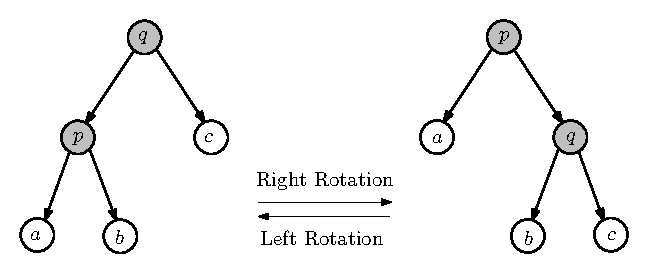
\includegraphics[width=6cm]{figs/treerotation}
\caption{\label{fig:treerotation}Left and right rotations of a BST.}
\end{center}
\end{figure}

\end{Example}

The precise details of exactly when a rotation is required, and which kind, 
differ depending on the type of balanced BST. In each case the programming of
the insertion and removal operations is quite complex, as is the analysis. 
We will not go into more details here---the reader should consult the  
recommended references.

Balancing of AVL trees requires extra memory and heavy
computations. This is why even more relaxed efficient balanced search
trees such as red-black trees are more often used in practice.

\begin{Definition}
A \defnfont{red-black tree} is a binary search tree such that 
every node is coloured either red or black, and every non-leaf node 
has two children. In addition, it satisfies the following properties: 
\begin{itemize}
\item the root is black;
\item all children of a red node must be black;
\item every path from the root node to a leaf must contain the same number of 
black nodes.
\end{itemize}
\end{Definition}

\begin{Theorem}
If every path from the root to a leaf contains $b$ black 
nodes, then the tree contains at least $2^{b}-1$ black nodes.
\end{Theorem}
\begin{proof}

The statement holds for $b=1$ (in this case
the tree contains either the black root only or the black
root and one or two red children). In line with the induction hypothesis, 
let the statement hold for all red-black trees with $b$ black nodes  in every 
path. If a tree contains $b+1$ black nodes in every path and has two black 
children of the root, then the tree contains two subtrees with $b$ black nodes 
just under the root and has in total at least 1+$2 \cdot(2^{b}-1) = 2^{b+1}-1$ 
black nodes. If the root has a red child, the latter has only black children, 
so that the total number of the black nodes can become even larger. 
\end{proof}

Each path cannot contain two consecutive red nodes and increase more
than twice after all the red nodes are inserted. Therefore, the height
of a red-black tree is at most $2\lceil \lg n \rceil$, and the
search in it is logarithmic, $O(\log n)$.

Red-black trees allow for a very fast search. This data structure has
still no precise analysis of its average-case performance. Its
properties are found either experimentally or by analysing red-black
trees containing random $n$ keys. There are about $\lg n$ comparisons per search 
on the average and fewer than $2\lg n + 2$ comparisons in the
worst case. Restoring the tree after insertion or deletion of single node 
requires $O(1)$ rotations and $O(\log n)$ colour changes in the worst case.

Another variety of balanced tree, the \defnfont{AA-tree}, becomes more efficient 
than a red-black tree when node deletions are frequent. An AA-tree has 
only one extra condition with respect to a red-black tree, namely that 
the left child may not be red. This property simplifies the removal 
operation considerably.

\subsection{Balanced B-trees: efficiency of external search}
\label{ss:B-tree}

The B-tree is a popular
structure for ordered databases in external memory such as magnetic or
optical disks. The previous ``Big-Oh'' analysis is invalid here because
it assumes all elementary operations have equal time complexity. This
does not hold for disk input / output where one disk access corresponds
to hundreds of thousands of computer instructions and the number of
accesses dominates running time. For a large database of many millions
of records, even logarithmic worst-case performance of red-black or
AA-trees is unacceptable. Each search should involve a very small number
of disk accesses, say, 3--4, even at the expense of reasonably
complex computations (which will still take only a small fraction of a disk access time).

Binary tree search cannot solve the problem because even 
an optimal tree has height $\lg n$. To decrease the
height, each node must have more branches. The height of an
optimal $m$-ary search tree ($m$-way branching) is roughly
$\log_{m} n$ (see Table~\ref{tbl:m-ary:branch}), or  
$\lg m$ times smaller than with an optimal binary tree 
(for example, $6.6$ times for $m=100$).

\begin{table}[htb!]
\caption{\label{tbl:m-ary:branch}Height of the optimal $m$-ary 
search tree with $n$ nodes.}
\centerline{
\begin{tabular}{|c|r|r|r|r|r|} \hline 
$n$ & $10^{5}$ & $10^{6}$ & $10^{7}$ & $10^{8}$  & $10^{9}$ \\ \hline
$\lceil \log_{2}n \rceil$  & 17  & 20  & 24  & 27  & 30 \\ \hline 
$\lceil \log_{10}n \rceil$ & 5   & 6   & 7   & 8   & 9 \\ \hline 
$\lceil \log_{100}n \rceil$ & 3   & 3   & 4   & 4   & 5 \\ \hline
$\lceil \log_{1000}n \rceil$ & 2   & 2   & 3   & 3   & 3 \\ \hline
\end{tabular}}
\end{table}

\begin{figure}[htb]
\begin{center}
\illustr{mtr-ex.ps}{90mm}
\caption{\label{mtr-ex} Multiway search tree of order $m=4$.}
\end{center}
\end{figure}

Figure~\ref{mtr-ex} shows that the search and the traversal of a
multiway search tree generalize in a straightforward way the binary
search tree operations. If in the latter case the search key is compared
to a single key in a node in order to choose one of two branches or stop
in the node, in an $m$-ary tree, the search key is compared to at most
$m-1$ keys in a node to choose one of $m$ branches. The major difference
is that multiple data records are now associated only with leaves
although some multiway trees do not strictly follow this condition. Thus
the worst-case and the average-case search involve the tree height and
the average leaf height, respectively.

\begin{Example}
Search for a desired key $k$ in Figure~\ref{mtr-ex} is guided by
thresholds, for example at the root it goes left if $k<4$, down if $4
\le k < 10$, and right if $k \ge 10$. The analogous comparisons are
repeated at every node until the record with the key $k$ is found at a
leaf or its absence is detected. Let $k=17$. First, the search goes
right from the root (as $17 > 10$), then goes to the third child of the
right internal node (as $17 \le 17 < 20$), and finally finds the desired
record in that leaf.
\end{Example}

\begin{Definition}
A \defnfont{B-tree} of order $m$ is an $m$-ary tree such that:
\begin{itemize} 
\item the root is either a leaf or it has between $2$ and
$m$ children inclusive; 
\item each nonleaf node (except possibly the root) has
between $\lceil m/2 \rceil$ and $m$ children inclusive;
\item each nonleaf node with $\mu$ children has $\mu-1$
keys, $(\theta[i]: i=1,\ldots,\mu-1)$, to guide the search where $\theta[i]$ is the smallest key in subtree $i+1$;
\item all leaves are at the same depth;
\item data items are stored in leaves, each storing between $\lceil l/2 \rceil$ and $l$ items, for some $l$.
\end{itemize} 
\end{Definition}

Other definitions of B-trees (mostly with minor changes) also exist, but
the above one is most popular. The first three conditions specify the
memory space each node needs (first of all, for $m$ links and $m-1$
keys) and ensure that more than half of it, except possibly in the root,
will be used. The last two conditions form a well-balanced tree.

\begin{figure}[htb]
\begin{center}
\illustr{mtr-b4.ps}{90mm}
\caption[2--4 B-tree with the leaf storage size 7.]%
{2--4 B-tree with the leaf storage size 7
($2..4$ children per node and $4..7$ data items per leaf).}
\label{mtr-b4} 
\end{center}
\end{figure}

\begin{note}
B-trees are usually named by their \defnfont{branching limits}, 
that is, $\lceil m/2 \rceil$--$m$, so that $2$--$3$ and $6$--$11$ 
trees are B-trees with
$m=3$ and $m=11$, respectively.
\end{note}

\begin{Example} In a
$2-4$ B-tree in Figure~\ref{mtr-b4} 
all nonleaf nodes have between 
$\lceil 4/2 \rceil = 2$ and $4$ children and thus from
$1$ to $3$ keys. The number $l$ of 
data records associated with a leaf depends on 
the capacity of external memory and the record size. 
In Figure~\ref{mtr-b4}, $l=7$ and each leaf stores between 
$\lceil 7/2 \rceil = 4$ and $7$  data items.
\end{Example}

Because the nodes are at least half full, a  B-tree with $m \ge 8$
cannot be a simple binary or ternary tree. Simple ternary $2$--$3$ B-trees
with only two or three children per node are sometimes in use for
storing ordered symbol tables in internal computer RAM. But branching
limits for B-trees on external disks are considerably greater to make
one node fit in a unit data block on the disk. Then the number of nodes
examined (and hence the number of disk accesses) decreases $\lg m$
times or more compared with a binary tree search.

In each particular case, the tree order $m$ and the leaf capacity $l$ 
depend on the disk block size and the size of records to
store. Let one disk block hold $d$ bytes, each key be of
$\kappa$ bytes, each branch address be of \(b\) bytes, 
and the database contain $s$ records, each of size $r$ bytes.
In a B-tree of order $m$, each nonleaf node stores at most $m-1$ keys 
and $m$ branch addresses, that is,
in total, $\kappa(m-1)+bm = (\kappa + b) m -\kappa$ bytes. 
The largest order $m$
such that one node fits in one disk block,
$(\kappa+b)m -\kappa \le d$, is 
$m=\left\lfloor \frac{d+\kappa}{b+\kappa}\right\rfloor$.
Each internal node, except the root,
has at least $\left\lceil \frac{m}{2} \right\rceil$ branches.
At most $l=\frac{d}{r}$ records fit in one block, and
each leaf addresses from $\frac{l}{2}$ to $l$ records. 
Assuming each leaf is full, the total number of the
leaves is $n = \left\lceil \frac{s}{l} \right\rceil$, so that
in the worst case the leaves are at level 
$\lceil \log_{m/2} n\rceil +1$.

\begin{Example}\label{exm:btree}
Suppose the disk block is $d=2^{15}\equiv 32768$ bytes, 
the key size is $\kappa=2^{6}\equiv 64$ bytes, the branch 
address has \(b=8\) bytes, and the
database contains $s=2^{30}\cong 1.07\cdot 10^9$ records
of size $r=2^{10}\equiv 1024$ bytes each. Then
the B-tree order is 
$m=\lfloor \frac{32768+64}{8+64} \rfloor =
\lfloor \frac{32832}{72} \rfloor = 456$ so that each internal node, 
except the root, has at least 228 branches.
One block contains at most $l=\frac{32768}{1024}=32$ records,
and the number of leaves is at least 
$n = \left\lceil 2^{30}/32 \right\rceil = 2^{25}$. The
worst-case level of the leaves in this B-tree is 
$\lceil \log_{228} 2^{25}\rceil +1 = \lceil 3.19 \rceil +1 = 5$.
\end{Example}

Generally, a search in or an insertion into a B-tree of order $m$ with $n$
data records requires fewer than $\lceil \log_{m/2}n \rceil$ disk
accesses, and this number is practically constant if $m$ is sufficiently
big as shown in Table~\ref{tbl:m-ary:branch}. The running time becomes
even smaller if the root and the upper two tree levels are stored in
internal RAM and the slow disk accesses occur only for level 3 or
higher. The three-level B-tree with $m=456$ can handle up to $456^{3}$,
or $94,818,816$ entries. If in Example~\ref{exm:btree} each key uses
only \(\kappa=24\) bytes, then $m = 1024$, and the three-level tree can
handle over $10^9$ entries.

Data insertion into a B-tree is simple if the corresponding leaf is not
already full. A full leaf has to be split into two leaves, both having
the minimum number of data items, and the parent node should be updated.
If necessary, the splitting propagates up until it finds a parent that
need not be split or reaches the root. Only in the extremely rare case
that the root has to be split, the tree height increases and a new root
with two children (halves of the previous root) is created. Data
deletion is also simple until the leaf is empty and its neighbours must
be combined to form a full leaf. Although the programming is not simple, all
changes are well defined. Algorithm analysis, beyond the scope of this
book, shows that both data insertion,
deletion, and retrieval have only about $\log_{\frac{m}{2}} n$ disk
accesses in the worst case.

\subsection*{Exercises}

\begin{Exercise}\label{exr:redblack:example}
Draw two different red-black trees containing at most two black nodes 
along every path from the root to a leaf.
\end{Exercise}


\begin{Exercise}\label{exr:avl:example}
Draw two different AVL trees of size $n=7$ and compare
them to the complete binary tree of the same size. Is
the latter also an AVL tree?
\end{Exercise}



\begin{Exercise}\label{exr:aa:example}
Draw an AA-tree containing at most 2 black nodes 
along every path from a node to a leaf and differing from
the complete binary tree of order \(n=7\).
\end{Exercise}

\begin{Exercise}\label{exr:rotation}
Draw a binary search tree of minimum size such that a left rotation 
reduces the height of the tree.
\end{Exercise}

\section{Hash tables}\label{sec:hash:tables}

There are numerous ways to implement the table ADT. We have already seen 
that various search trees will do everything required, provided the keys are 
from some totally ordered set. If, say, the keys are dictionary words with the 
usual ordering, then it is not necessary to use any integer encoding---keys can 
be compared directly.

Suppose now that we have a very simple situation where the number of 
possible keys is small. Then  we can just store the values in an array. 
One array entry can be reserved in advance for each possible key, and the 
key-to-value mapping ends up as a conventional array address. Searching then 
has worst-case constant time, as does insertion and deletion. This 
implementation of a table works well provided the number of possible keys is 
sufficiently small.

However, that nice state of affairs does not occur often (we could use it 
for the airport codes in  Example~\ref{exm:adt:airports}). Usually there exists 
a very large number of possible keys although only a tiny fraction of them are
actually put into use. For example, suppose that we have a database where each 
customer is identified by an 8-digit telephone number. If we have 10 000 customers, 
only $0.01\%$ of the array addresses are filled.

There is another technique to store and search for
values in symbol tables, called {\defnfont{hashing}}, that uses less space and 
retains many (not all) of the benefits of direct array addressing. 

\begin{Definition}
Hashing computes an integer \defnfont{hash code} for each object using a 
\defnfont{hash function} that maps objects (for example, keys) to indices of 
a given linear array (the \defnfont{hash table}). 
\end{Definition}

Hash functions are designed in such a manner that hash codes are
computed quickly. The computation  of an array index with 
a hash function, or ``hashing a key to an index'',
depends only on the key to hash and is independent of other keys in the table.
 If \(h(k)\) is the value of a hash function for $k$, then the
 key \(k\) should be placed at location \(h(k)\).

The hash function is chosen so as to always return a valid index 
for the array. A \defnfont{perfect hash function} maps each key to a different 
index. Unfortunately, it is difficult to find such a function in most cases. 

\begin{Example} \label{exm:hashing}
Let us map two-digit integer keys onto the ten array indices 
[0, 1, \ldots, 9] by a
simple hash function \(h(k) = \lfloor k/10 \rfloor\). Then the keys \(21\) and
\(27\) both have the hash code \(2\) pointing to
the same position in the array. Such a situation in which two different keys, 
\(k_{1} \ne k_{2}\), hash to the same index (table address), 
\(h(k_{1}) = h(k_{2})\), is called a \defnfont{collision}. Because both
table entries \((k_{1},v_{1})\) and \((k_{2},v_{2})\) cannot
be at the same address, we need a  definite {\defnfont{collision resolution policy}}. 
\end{Example}

Different keys hashed to the same hash address are  called \defnfont{synonyms}, 
and data items with synonymic keys are frequently also referred to as 
synonyms. 

\subsection{Collision resolution: OALP, OADH, and SC hash tables}

There are many collision resolution policies. The main issues are:

\begin{itemize}
\item Do we use extra storage, or not?
\item Which element moves when a collision occurs: the incumbent element or the 
newcomer (or both)?
\item How do we decide where to move the evicted element to?
\end{itemize}

\subsubsection{Chaining}

In \defnfont{separate chaining} synonyms with the same hash address are stored 
in a linked list connected to that address.  We still hash the key of 
each item to obtain an array index. But if there is a collision, 
the new item is simply placed in this hash address, along with all other
synonyms. Each array element is a head reference for the associated linked 
list, and each node of this list stores not only the key and data
values for a particular table entry but also a link to the
next node. The head node of the list referenced by the array
element always contains the last inserted item.

\subsubsection{Open addressing}

Open addressing uses no extra space for collision resolution. Instead, 
we move one of the colliding elements to another slot in the array. We may use
LIFO (last-in, first out --- the new element must move), FIFO (first in, first out 
--- the old element must move), or more complicated methods such as Robin Hood 
or cuckoo hashing (see Notes). For our purposes here, we use LIFO.

Each collision resolution policy \defnfont{probes} another array slot, and if 
empty inserts the currently homeless element. If the probed slot is not empty, we probe 
again to find a slot in which to insert the currently homeless element, and so on 
until we finish insertion. The \defnfont{probe sequence} used can be a simple 
fixed sequence, or given by a more complicated rule (but is always deterministic).
They all have the property that they ``wrap around" the array when they reach the 
end. The two most common probing methods are:
\begin{itemize}
\item (Linear probing) always probe the element to the left;
\item (Double hashing) probe to the left by an amount determined by the value of 
a secondary hash function.
\end{itemize}

\begin{note}
The choice of probing to the left versus probing to the right is clearly a 
matter of convention; the reader should note that other books may use rightward
probing in their definitions.
\end{note}

\begin{table}[hbt]
\begin{center}
\caption{Open addressing with linear probing (OALP).}\label{hash-lin} 
\begin{tabular}{|c|c|c|l|} \hline 
\textbf{Data} [key,value] & \textbf{Hash}: key/10 & \textbf{Table address} & \textbf{Comments} \\ \hline
~[20,A] & 2 & 2 & \\
~[15,B] & 1 & 1 & \\
~[45,C] & 4 & 4 & \\
~[87,D] & 8 & 8 & \\
~[39,E] & 3 & 3 & \\
~[31,F] & 3 & 0 & try 3, 2, 1, 0 \\
~[24,G] & 2 & 9 & try 2, 1, 0, 9 \\ \hline
\end{tabular}
\end{center}
\end{table}

\begin{Example}\label{exm:lin:probing}
Table~\ref{hash-lin} shows how OALP fills the hash table 
of size 10 using the two-digit keys and the hash function
of Example~\ref{exm:hashing}. The first five insertions have found
empty addresses. However, the key--value 
pair [31, F] has a collision because the address 
\(h(31) = 3\) is already occupied by the pair [39, E] with the same
hash address, \(h(39) = 3\). Thus, the 
next lower table address, location 2, is probed to see if
it is empty, and in the same way the next locations 1
and 0 are checked. The address 0 is empty so that the pair [31, F]
can be placed there. 

A similar collision occurs when we try to insert the next
pair, [24, G], because the hash address \(h(24)=2\) for
the key 24 is already occupied by the previous pair [20, A]. 
Consequently,  we probe successive lower locations 1 and 0, and 
since they both are already
occupied, we wrap around and continue the search at the highest
location 9. Because it is empty, the pair [24, G] is inserted in this location 
yielding the final configuration given in Table~\ref{hash-lin}.
\end{Example}

OALP is simple to implement but the hash table may degenerate due to
\defnfont{clustering}. A \defnfont{cluster} is a
sequence of adjacent occupied table entries. OALP tends to form clusters 
around the locations
where one or more collisions have occurred. Each
collision is resolved using the next empty location 
available for sequential probing. Therefore, other collisions 
become more probable in that neighbourhood, and the larger the
clusters, the faster they grow. As a result,
a search for an empty address to place a collided key may
turn into a very long sequential search. 

Another probing scheme, \defnfont{double hashing}, reduces the 
likelihood of clustering. In double hashing, when a collision occurs, the key
is moved by an amount determined by a secondary hash function \(\Delta\).  Let \(h\) denote
the primary hash function. Then for each key \(k\) we have the starting probe 
address \(i_{0} = h(k)\) and the probe decrement \(\Delta(k)\). Each
next successive probe position is 
\(i_{t} = ( i_{t-1} - \Delta(k) ) \bmod m\); \
\(t=1,2,\ldots\) where $m$ is the table size.

\begin{Example}\label{exm:double:hashing}
Table~\ref{hash-dbl} shows how OADH fills the same hash table as in
Example~\ref{exm:lin:probing} if the 
hash function is given by \(\Delta(k) = (h(k) + k) \bmod 10\).

\begin{table}[hbt]
\begin{center}
\caption{\label{hash-dbl} Open addressing with double hashing (OADH).}
\begin{tabular}{|c|c|c|l|} \hline 
\textbf{Data} [key,value] & \textbf{Hash}: key/10 & \textbf{Table address} & \textbf{Comments} \\ \hline
~[20,A] & 2 & 2 & \\
~[15,B] & 1 & 1 & \\
~[45,C] & 4 & 4 & \\
~[87,D] & 8 & 8 & \\
~[39,E] & 3 & 3 & \\
~[31,F] & 3 & 9 & using $\Delta(31)=4$ \\
~[24,G] & 2 & 6 & using $\Delta(24)=6$ \\ \hline
\end{tabular}
\end{center}
\end{table}

Now when we try to place the key--value 
pair [31, F] into position \(h(31) = 3\), the collision 
is resolved by probing the table locations with decrement
\(\Delta(31) = 4\). The first position, \((3-4)\mod 10 = 9\) is
empty so that the pair [31, F] can be placed there. 
For the collision of the pair, [24, G], at location 2 
the decrement \(\Delta(24) = 6\) immediately leads to
the empty location $6$. The final table
in Figure~\ref{hash-dbl} contains three small clusters 
instead of one large
cluster in Figure~\ref{hash-lin}. 
\end{Example}

Generally, OADH results in more uniform hashing that
forms more clusters than OALP but of smaller sizes.
Linear probing extends each cluster from its end with
the lower table address, and nearby clusters join into
larger clusters growing even faster. Double hashing does
not extend clusters only at one end and does not tend
to join nearby clusters.



\subsection{Analysis of hash tables}

The time complexity of searching in and inserting items in a
hash table of size \(m\) with
\(n\) already occupied entries is determined by the \defnfont{load factor},
  \(\lambda := \frac{n}{m}\). In open addressing, \(0 \le \lambda < 1\): $\lambda$
  equals the fraction of occupied
slots in the array, and cannot be exactly equal to 1 because a hash table 
should have at least one empty entry in order to efficiently terminate the search 
for a key or the insertion of a new key.

Open addressing and separate chaining require $n$ probes in the worst case, 
since all elements of the hash table may be synonyms. However the basic intuition
is that provided the table is not too full, collisions should be rare enough that
searching for an element requires only a constant number of probes on average.

Thus we want a result such as: ``\emph{Provided the load factor is kept bounded 
(and away from 1 in the case of open addressing), all operations in a hash table 
take $\Theta(1)$ time in the average case.}"

In order to have confidence in this result, we need to describe our mathematical model of 
hashing. Since a good hash function should scatter keys randomly, and we have no
knowledge of the input data, it is natural to use the ``random balls in bins" 
model. We assume that we have thrown $n$ balls one at a time into $m$ bins, 
each ball independently and uniformly at random. 

For our analysis, it will be useful to use the function $Q$ defined below.
 
\begin{Definition}
For each integer $m, n$ with $1 \leq n \leq m$, we define 
$$
Q(m,n) = \frac{m!}{(m-n)! m^n} = \frac{m}{m} \frac{m-1}{m} \dots 
\frac{m - n + 1}{m}.
$$
Note that $Q(m,1) = 1$.
\end{Definition}

\subsubsection{Basic analysis of collisions}

It is obvious that if we have more items than the size of the hash table, at least 
one collision must occur. But the distinctive feature of collisions is that they 
are relatively frequent even in almost empty hash tables. 

The \defnfont{birthday paradox} refers to the following surprising fact:
\emph{if there are 23 or more people in a room, the chance is greater than 50\%
that two or more of them have the same birthday.} Note: this is not a paradox 
in the sense of a logical contradiction, but just a ``counter-intuitive" 
fact that violates ``common sense".

More precisely, if each of 365 bins
is selected with the same chance \(\frac{1}{365}\), then after
23 entries have been inserted, the probability that at least one collision has 
occurred (at least one bin has at least two balls) is more than 50\%. 
Although the table is only $23/365$ ($\cong 6.3\%$) full,
more than half of our attempts to insert one more entry will result in a collision!

Let us see how the birthday paradox occurs. Let \(m\) and \(n\) denote the 
size of a table and the number of items to insert, respectively. 
Let $\Pr_{m}(n)$ be the probability of at least one collision when 
$n$ balls are randomly placed into  $m$ bins.

\begin{Lemma}
The probability of no collisions when $n$ balls are thrown independently 
into $m$ boxes uniformly at random is $Q(m, n)$. Thus 
${\Pr_m}(n) =  1 - Q(m,n)$
and the expected number of balls thrown until the first collision is 
$\sum_{n\leq m} Q(m,n)$. 
\end{Lemma}

\begin{proof} Let $\pi_{m}(n)$ be the probability of no collisions.
 The ``no collision'' event after
inserting \(\nu\) items; \(\nu=2,\ldots,n\), is a joint event of
``no collision'' after inserting the preceding \(\nu-1\) items and 
``no collision'' after inserting one more item, given \(\nu-1\)
positions are already occupied. Thus 
\(\Pr_m(\nu)=\Pr_m(\nu-1)P_{m}(\mathrm{no~collision} \mid \nu-1)\)
where \(P_{m}(\mathrm{no~collision} \mid \nu)\) denotes the conditional
probability of no collision for a single item inserted into the
table with \(m-\nu\) unoccupied positions. This latter
probability is simply \(\frac{m-\nu}{m}\).

This then yields immediately
\[
\pi_{m}(n) = \frac{m}{m}\frac{m-1}{m} \dots \frac{m-n+1}{m} = 
\frac{m(m-1)\cdots(m-n+1)}{m^{n}} =  \frac{m!}{m^{n}(m-n)!}
\]
Therefore,
\(
\Pr_{m}(n) = 1 - \frac{m!}{m^{n}(m-n)!} = 1 - Q(m,n)
\)
which gives the first result.

The number of balls is at least $n+1$ with probability $Q(m,n)$. Since the 
expected value of a random variable $T$ taking on nonegative integer values 
 can always be computed by $E[T] = \sum_{n\geq 1} i \Pr(T=i) = 
 \sum_{j\geq 0} \Pr(T>j)$, and these latter probabilities are zero when $j>m$,
 the second result follows.
\end{proof}

Table~\ref{adt-tbl2} presents (to 4 decimal places)
some values of \(\Pr_{m}(n)\) for \(m=365\) and \(n=5\ldots100\). 
As soon as $m=47$ (the table with 365 positions is only 12.9\% full),
the probability of collision is greater than 0.95.
Thus collisions are frequent even in sparsely occupied tables.

\begin{table}[hbt!]
  \caption{\label{adt-tbl2} Birthday paradox: $\Pr_{365}(n)$.}
 \centerline{
  \begin{tabular}{|c|r|r|r|r|r|r|r|} \hline
    \(n\)          & 5 & 10 & 15 & 20 & 22  \\ \hline 
    \(\Pr_{365}(n)\) & 
       0.0271 & 0.1169 & 0.2529 & 0.4114 & 0.4757 \\
    \hline\hline 
    \(n\)          & 23 & 25 & 30 & 35 & 40  \\ \hline 
    \(\Pr_{365}(n)\) & 
       0.5073 & 0.5687 & 0.7063 & 0.8144 & 0.8912 \\
    \hline\hline 
    \(n\)          & 45 & 50 & 55 & 60 & 65  \\ \hline 
    \(\Pr_{365}(n)\) & 
       0.9410 & 0.9704 & 0.9863 & 0.9941 & 0.9977 \\
    \hline\hline 
    \(n\)          & 70 & 75 & 80 & 90 & 100  \\ \hline 
    \(\Pr_{365}(n)\) & 
       0.9992 & 0.9997 & 0.9999 & 1.0000 & 1.0000 \\
    \hline
  \end{tabular}}
\end{table}

Figure~\ref{fig:birthday} shows the graph of $\Pr_{365}(n)$ as a function of $n$.
The median of this distribution occurs around $n=23$, as we have said above, and
so 23 or more balls suffice for the probability of a collision to exceed 1/2. 
Also, the expected number of balls before the first collision is easily computed
to be 25. 

\begin{figure}
\begin{center}
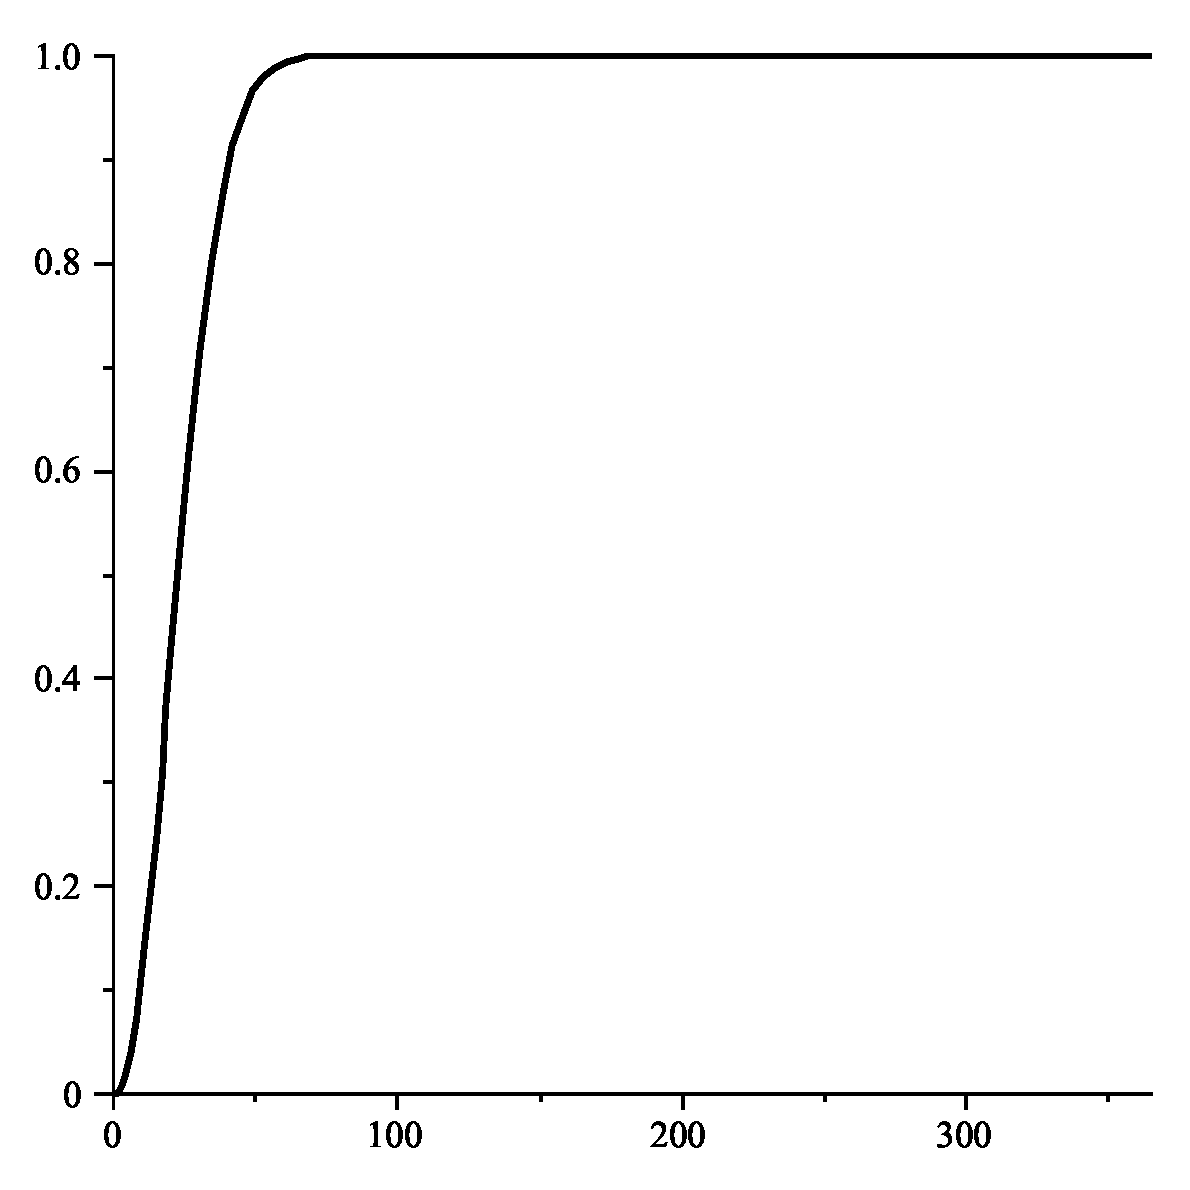
\includegraphics[width=6cm]{figs/birthday365.eps}
\end{center}
\caption{\label{fig:birthday} Birthday paradox: $\Pr_{365}(n)$.}
\end{figure}

When the load factor is much less than $1$, the average number of balls per bin
is small. If the load factor exceeds $1$ then the average number is large. In 
each case analysis is not too difficult. For hashing to be practical, we need 
to be able to fill a hash table as much as possible before we spend valuable 
time \defnfont{rehashing} --- that is, allocating more space for the table
 and reassigning hash codes via a new hash function. Thus we need to analyse 
 what happens when the load factor is comparable to $1$, that is, when the 
 number of balls is comparable to the number of bins. This also turns out to be
 the most interesting case mathematically.

\subsubsection{Theoretical analysis of hashing}

In addition to the basic operations for arrays, we also 
consider the computation of the hash address of an item to be an elementary 
operation.

Chaining is relatively simple to analyse. 

\begin{Lemma}\label{lem:sc}
The expected running time for unsuccessful search
in a hash table with load factor \(\lambda\) using
separate chaining is given by 
$$T_{\mathrm{us}}(\lambda)= 1+\lambda. $$
The expected running time for successful search is $O(1 + \lambda/2)$.

Update, retrieval, insertion and deletion all take time that is $O(1+\lambda)$.
\end{Lemma}
\begin{proof}
In an unsuccessful search for a key \(k\), the computation of
the hash address, \(h(k)\), takes one elementary
operation. The average running time to unsuccessfully search for the
key at that address is equal to the average length of the
associated chain, \(\lambda=\frac{n}{m}\). Thus in total
$T_{\mathrm{us}}(\lambda) = 1 + \lambda = 1 + n/m$.

The result for successful search and other operations 
now follows from Lemma~\ref{lem:ss-us}, since update, retrieval and deletion from a 
linked list take constant time.
\end{proof}

To analyse open addressing, we must make some extra assumptions. We use the 
\defnfont{uniform hashing hypothesis}: each configuration of $n$ keys in a 
hash table of size $m$ is equally likely to occur. This is what we would expect 
of a truly ``random" hash function, and it seems experimentally 
to be a good model for double hashing. Note that this is stronger than just 
requiring that each key is independently and uniformly likely to hash initially 
to each slot before collision resolution (``random balls in bins").
It also implies that all probe sequences are equally likely.

\begin{Lemma}\label{lem:oadh}
Assuming the uniform hashing hypothesis holds, 
the expected number of probes for search in a hash table satisfy
$$
T_{\mathrm{us}}(\lambda) \leq \frac{1}{1-\lambda} 
$$
and
$$ 
T_{\mathrm{ss}}(\lambda) \leq \frac{1}{\lambda} \ln \frac{1}{1-\lambda}.
$$
\end{Lemma}

\begin{proof} 
The average number of probes for an
unsuccessful search is
\(
T_{\mathrm{us}}(\lambda) = \sum_{i=1}^{n}i p_{m,n}(i)
\)
where \(p_{m,n}(i)\) denotes the probability of exactly \(i\)
probes during the search. Obviously, 
\(p_{m,n}(i) = \Pr (m,n,i) - \Pr (m,n,i+1)\) where 
\(\Pr (m,n,i)\) is the probability of \(i\) or more probes
in the search. By a similar argument to that used in the
birthday problem analysis we have for $i\geq 2$
$$
\Pr (m,n,i) = \frac{n}{m}\cdot \frac{n-1}{m-1} \cdots \frac{n-i+2}{m-i+2}
$$
while $\Pr (m,n,1) = 1$.
Note that clearly $\Pr (m,n,i) \leq (n/m)^{i-1} = \lambda^{i-1}.$
Thus
\begin{eqnarray*}
T_{\mathrm{us}}(\lambda) & = &
\sum\limits_{i=1}^{n}i\left ( 
{\textstyle \Pr (n,m,i) - \Pr (n,m,i+1) }\right ) \\
& \le &
\sum\limits_{i=1}^{\infty}i\left ( 
{\textstyle \Pr (n,m,i) - \Pr (n,m,i+1)}\right ) 
= \sum\limits_{i=1}^{\infty} \Pr (n,m,i) 
\le  
\sum\limits_{i=1}^{\infty} \lambda^{i-1} = \frac{1}{1-\lambda} = \frac{m}{m-n}.
\end{eqnarray*}

The result for successful search now follows by averaging. We have
\begin{align*}
T_{\mathrm{ss}}(\lambda) & \leq \frac{1}{n} \sum_{i=0}^{n-1} \frac{m}{m-i} \\
& = \frac{1}{\lambda} \sum_{j=m-n+1}^m \frac{1}{j}\\
& \leq \frac{1}{\lambda} \int_{n-m}^n dx/x = \frac{1}{\lambda} \ln\left(\frac{m}{m-n}\right) = \frac{1}{\lambda}
\ln\left(\frac{1}{1-\lambda}\right).
\end{align*}
\end{proof}

\begin{note}
It can be shown that the exact values are
\begin{align*}
T_{\mathrm{us}}(\lambda) & = \frac{m+1}{m-n+1} \approx \frac{1}{1-\lambda}\\
T_{\mathrm{ss}}(\lambda) & = \frac{m+1}{n} \left( H_{m+1} - H_{m-n+1} \right) 
\approx \frac{1}{\lambda} \ln\left(\frac{1}{1-\lambda}\right)
\end{align*}
so that the upper bounds in the theorem are asymptotically precise as $m\to \infty$.
\end{note}

Good implementations of OADH have been shown in theory and practice to be well 
described by the simple uniform hashing model above, so we may safely use the above
results. 

However, OALP is not well 
described by the uniform hashing model, because of its clustering 
behaviour. It can be analysed, however, in a similar but more complicated manner.

\begin{Lemma}\label{lem:oalp}Assuming uniformly hashed random input,
the expected number of probes for successful, $T_{\mathrm{ss}}(\lambda)$,
and unsuccessful, $T_{\mathrm{us}}(\lambda)$, search in a hash table using 
OALP are, respectively, 
\[
T_{\mathrm{ss}}(\lambda)\approx
0.5 \left ( 1 + \frac{1}{1-\lambda}\right ) 
\; \;\;\; 
\mathrm{and}
\; \;\;\; 
T_{\mathrm{us}}(\lambda)\approx
0.5 \left ( 1 + \left ( \frac{1}{1-\lambda} \right )^2 \right )
\]
\end{Lemma}
\begin{proof}
The proof is beyond the scope of this book (see Notes).
\end{proof}

The relationships in Lemma~\ref{lem:oalp} and Lemma~\ref{lem:oadh}
completely fail when \(\lambda=1\). But the latter situation indicates a full 
hash table, and we should avoid getting close to it anyway. 

Unlike OALP and OADH, the time estimates for separate chaining (SC) remain
valid with data removals. Because each chain may keep several 
table elements, the load factor may be more than $1$.

\begin{table}[htb!]
  \caption{\label{tbl-hash}Average search time bounds in hash tables with
           load factor $\lambda$.} 
 \centerline{
  \begin{tabular}{|c|ccc|ccc|} \hline
   \(\lambda\) & 
   \multicolumn{3}{c|}{Successful search: $T_{\mathrm{ss}}(\lambda)$} &
   \multicolumn{3}{c|}{Unsuccessful search: $T_{\mathrm{us}}(\lambda)$} 
   \\ \cline{2-7}
               & \textbf{SC} & \textbf{OALP} & \textbf{OADH} 
               & \textbf{SC} & \textbf{OALP} & \textbf{OADH}\\ \hline
0.10 & 1.05 & 1.06 & 1.05 & 1.10 & 1.12 & 1.11 \\
0.25 & 1.12 & 1.17 & 1.15 & 1.25 & 1.39 & 1.33 \\
0.50 & 1.25 & 1.50 & 1.39 & 1.50 & 2.50 & 2.0 \\
0.75 & 1.37 & 2.50 & 1.85 & 1.75 & 8.50 & 4.0 \\
0.90 & 1.45 & 5.50 & 2.56 & 1.90 & 50.5 & 10.0 \\
0.99 & 1.49 & 50.5 & 4.65 & 1.99 & 5000.0 & 100.0 \\ \hline
  \end{tabular}}
\end{table}

Table~\ref{tbl-hash} presents the above theoretical 
estimates of the search time in the OALP, OADH, and SC hash tables under 
different load factors. Average time measurements for actual hash
tables~\cite{standish} are close to the estimates for SC tables in  the whole
range \(\lambda \le 0.99\) and seem to be valid for larger
values of \(\lambda\), too. The measurements for OADH tables
remain also close to the estimates up to  \(\lambda = 0.99\).
But for OALP tables, the measured time is considerably
less than the estimates if \( \lambda > 0.90\) for a successful search and 
\( \lambda > 0.75\) for an unsuccessful search.

\begin{Example}
The expected performance of hashing depends only on the load factor.
If \(\lambda = 0.9\), OADH 
double hashing takes on the average 2.56 and 10 probes for 
successful and unsuccessful search, respectively. But 
if \(\lambda = 0.5\), that is, the same keys are stored 
in a roughly twice larger table, the same numbers decrease
to 1.39 and 2 probes.
\end{Example}


\subsection{Implementation of hashing}

\subsubsection{Resizing} 
One problem with open addressing is that successive insertions may cause the table
to become almost full, which degrades performance. Eventually we will need to 
increase the table size. Doing this each time an element is inserted is very 
inefficient. It is better to use an upper bound, say $0.75$, on the load factor, 
and to double the array size when this threshold is exceeded. This will then require 
recomputing the addresses of each element using a new hash function.

The total time required to resize, when growing a table from $0$ to $m=2^k$ elements,
is of order $1 + 2 + 4 + 8 + \dots + 2^{k-1} = 2^k - 1 = m - 1$. Since the $m$ 
insertions take time of order $m$ (recall the table always has load factor 
bounded away from $1$), the average insertion time is still $\Theta(1)$.

\subsubsection{Deletion}

It is quite easy to delete a table entry from a hash table with separate 
chaining (by mere node deletion from a linked list). However, open addressing 
encounters difficulties. If a particular table entry is physically removed
from a OA-hash table leaving an empty entry in that place, the search for 
subsequent keys becomes invalid. This is because the OA-search terminates when 
the probe sequence encounters an empty table entry. Thus if a previously occupied 
entry is emptied, all probe sequences that 
previously travelled through that entry will
now terminate before reaching the right location. 

To avoid this problem, the deleted entry is normally marked in such a way that
insertion and search operations can treat it as an empty and 
nonempty location, respectively. Unfortunately, such a policy results in hash 
tables packed with entries which are marked as deleted. But in this case the 
table entries can be rehashed to preserve only actual data and really delete all
marked entries. In any case, the time to delete a table entry remains \(O(1)\) 
both for SC  and OA hash tables.

\subsubsection{Choosing a hash function}
\label{sec:choice:hash:fun} 

Ideally, the hash 
function, \(h(k)\), has to map keys uniformly and randomly onto 
the entire range of hash table addresses. Therefore, the
choice of this function has much in common with the choice of
a generator of uniformly distributed pseudorandom numbers. 
A randomly chosen key \(k\) has to equiprobably hash to each
address so that uniformly distributed keys produce uniformly
distributed indices \(h(k)\). A poorly designed hash function
distributes table addresses nonuniformly and tends to
cluster indices for contiguous clusters of keys. 
A well designed function scatters the keys as to avoid
their clustering as much as possible.

If a set of keys is fixed, there always exists a \defnfont{perfect hash function}
that maps the set one-to-one onto a set of table indices and thus entirely 
excludes collisions. However, the problem is how to design such a function as
it should be computed quickly but without using large tables.
There exist techniques to design perfect hash functions for given sets of keys. 
But perfect hashing is of very limited interest because in most applications 
data sets are not static and the sets of keys cannot be pre-determined.

Four basic methods for choosing a hash function
are \defnfont{division}, \defnfont{folding}, \defnfont{middle-squaring}, and 
\defnfont{truncation}.
\begin{description}
\item[Division] assuming the table size is a prime number \(m\) 
and keys, \(k\), are integers,
the quotient, \(q(k,m)=\left \lfloor \frac{k}{m} \right \rfloor \), 
and the remainder, \(r(k,m)=k \mod m\), of the integer division of
\(k\) by \(m\) specify the
probe decrement for double hashing and the value
of the hash function \(h(k)\), respectively:
$$
h(k) = r(k,m) \mbox{ and }
\Delta(k) = \max \left \{
1, \ q(k,m) \bmod m \right\} \quad . 
$$
The probe decrement is put to the range \([1,\ldots,m-1]\) because all
decrements should be nonzero and point to the indices
\([0,1,\ldots,m-1]\) of the table. The reason that $m$ should be prime is that 
otherwise some slots may be unreachable by a probe sequence: for example if 
$m=12$ and $\Delta(k) = 16$, only $3$ slots will be probed before the sequence
returns to the starting position.

\item[Folding] an integer key \(k\) is divided into sections and 
the value \(h(k)\) combines sums, differences, and products of
the sections (for example, a 9-digit decimal key, such as 
\(k=013402122\), can be split into three sections:
013, 402, and 122, to be added together for getting 
the value \(h(k)=537\) in the range \([0,\ldots,2997]\)).

\item[Middle-squaring] a middle section of an integer key
\(k\), is selected and squared, then a middle section of 
the result is the value \(h(k)\) (for example, the squared middle section, 402, of 
the above 9-digit key, \(k=013402122\), results in 161604, and
the middle four digits give the value \(h(k)=6160\) in the range
\([0,\ldots,9999]\)).

\item[Truncation] parts of a key are simply cut out and 
the remaining digits, or bits, or characters are used
as the value \(h(k)\)  
(for example, deletion of all but last three digits 
in the above 9-digit key, \(k=013402122\),
gives  
the value \(h(k)=122\) in the range \([0,\ldots,999]\)).
While truncation is extremely fast, the keys do not scatter
randomly and uniformly over the hash table indices. This is
why truncation is used together with other methods, but 
rarely by itself.
\end{description}

Many real-world hash functions combine some of the above methods.
                                            
We conclude by discussing the idea of \emph{universal hashing}. We have seen 
(in the section on quicksort) the idea of using randomization to 
protect against bad worst-case behaviour. An analogous idea works for hashing.
                                           
If a hash table is dynamically changing and its elements 
are not known in advance, any fixed hash function can result in 
very poor performance on certain inputs, because of collisions. 
Universal hashing allows us to reduce the probability of this occurrence
by randomly selecting the hash function at run time from a large set
of such functions. Each selected function still may be bad for a
particular input, but with a low probability
which remains equally low if the same input is met once again.
Due to its internal randomisation, universal hashing behaves well even for
totally nonrandom inputs. 

\begin{Definition}
Let \(K\), \(m\), and \(F\) denote
a set of keys, a size of a hash table (the range of indices),
and a set of hash functions mapping \(K\) to \(\{0,\ldots,m-1\}\),
respectively. Then \(F\) is a \defnfont{universal class} if any
distinct pair of keys \(k,\kappa \in {K}\)  collide
for no more than \(\frac{1}{m}\) of the functions in the class \({F}\),
that is,
\[
\frac{1}{|{F}|}
\left| \raisebox{10pt}{} \left\{ h \in {F} \mid \ h(k) = h(\kappa)\right\}\right|
\le \frac{1}{m} \quad .
\]
%where \(|Z|\) denotes cardinality of a finite
%set \({Z}\).

\end{Definition}
Thus in the universal class all key pairs behave well and the
random selection of a function from the class results in a probability of at most
\(\frac{1}{m}\) that any pair collide.

One popular universal class of hashing functions is produced by
a simple division method. It assumes the keys are integers and
cardinality of
the set of keys \({K}\) is a prime number larger 
than the largest actual key. The size \(m\) of the hash
table can be arbitrary. This universal class is described by
the next theorem.

\begin{Theorem}[Universal Class of Hash Functions] 
\label{the:ucf}
Let \({K}=\{0,\ldots,p-1\}\) and \(|{K}| = p\) be
a prime number. 
For any pair of integers \(a \in \{1, \ldots, p-1\}\)
and \(b \in \{0, \ldots, p-1\}\), let
\(
h_{a,b}(k) = \left ( (ak + b) \bmod p \right ) \bmod m
\).
Then
\[
{F} = \{h_{a,b} \mid \ 1 \le a < p \;\; \mathrm{and} \;\; 0 \le b < p \}
\]
is a universal class.
\end{Theorem}
\begin{proof}
It is easily shown that the number of collisions in the
class \({F}\), 
\[
\left| \raisebox{10pt}{} \{h\in {F} \mid  h(k)= h(\kappa); \ k,\kappa\in {K}\}\right|,
\]
is the number of distinct numbers \((x,y)\);
\(0 \le x,y < p\) such that 
\(x \bmod m = y \bmod m\). Let us denote the latter property: 
\(x \equiv y \pmod m\). %; (\hspace*{-3mm}\mod n)\).
It is evident that \(h_{a,b}(k) = h_{a,b}(\kappa)\) iff 
\[
(ak + b ) \bmod p  \equiv 
(a\kappa + b ) \bmod p  \pmod m \quad .
\]

Then for any fixed \(k, \kappa < p\), there is one-to-one
correspondence between the pairs \((a,b)\) such that
\(0 < a < p\) and \(0 < b < p\) and \(h_{a,b}(k) = h_{a,b}(\kappa)\),
and the pairs of distinct numbers \((x,y)\) with the
property that \(0 \le x,y < p\) and \(x \equiv y \pmod n\).
The correspondence is given in one direction by
\[
x = (ak + b) \bmod p; \;\; y = (a\kappa + b) \bmod p
\]
where \(x \ne y\) since 
\[
\{ az + b \mid \ z = 0, \ldots, p-1\} = \{0, \ldots, p-1\}
\]
when \(p\) is prime and \(a \ne 0\). In the other direction
the correspondence is given by the condition that \(a\) and
\(b\) are the unique integers in \(\{0, \ldots, p-1\}\) such
that
\[
ak + b \equiv x \pmod p \; \;\;\mathrm{and}\;\;\;
a\kappa + b \equiv y \pmod p \quad .
\]
These equations have a unique solution for \(a\) and \(b\)
since \(p\) is prime, and \(a \ne 0\) since \(x \ne y\).

Clearly \(|{F}| = p(p-1)\). Now let us find out how many 
pairs of distinct numbers
\((x,y)\) exist such that \(0 \le x,y < p\) and 
\(x \equiv y \pmod m\). For any fixed \(s < m\) there are
at most \( \left \lceil \frac{p}{m} \right \rceil \) numbers
\(x < p\) such that \(x \equiv s \pmod m\). Since \(p\) and
\(m\) are integers,
\(
\left \lceil \frac{p}{m} \right \rceil \le \frac{p-1}{m} +1
\).
Therefore for each \(x < p\) there are no more than
\(\frac{p}{m} -1 \le \frac{p-1}{m}\) numbers \(y < p\)
distinct from \(x\) such that \(x \equiv y \pmod m\), and
the total number of such pairs \((x,y)\) is at most 
\(\frac{p(p-1)}{m}\). Hence for any fixed distinct
pair of keys \((k,\kappa)\) the fraction of \({F}\)
that cause \(k\) and \(\kappa\) to collide is at
most \(\frac{1}{m}\), so the class \({F}\) is universal.
\end{proof}

This suggests the following strategy for 
choosing a hash function at run time: (i) find 
the current size of the set of keys to hash; 
(ii) select the next 
prime number \(p\) larger than the size of the key set found;
({iii}) randomly choose integers \(a\) and \(b\)
such that \(0 < a < p\) and \(0 \le b < p\), and 
({iv}) use the function \(h_{a,b}\) 
defined in Theorem~\ref{the:ucf}.


\subsection*{Exercises}

\begin{Exercise}\label{exr:java:hash}
The Java programming language (as of time of writing)
uses the following hash function $h$ for character strings. 
Each character has a Unicode value represented by an integer (for example, the 
upper case letters $A, B, \dots, Z$ correspond to $65, 66, \dots, 90$ and the 
lower case $a, b, \dots, z$ correspond to $97, 98, \dots, 122$). Then 
$h$ is computed using 32-bit integer addition via
$$h(s) = s[0]*31^{n-1} + s[1]*31^{n-2} + \dots + s[n-1]*31 + s[n].$$

Find two 2-letter strings that have the same hash value. How could you use this 
to make $2^{100}$ different strings all of which have the same hash code?
\end{Exercise}

\begin{Exercise}\label{exr:hash:oalp}
Place the sequence of keys \(k=10, 26, 52, 76, 13, 8, 3, 33, 60, 42\) 
into a hash table of size 13 using the modulo-based hash address \(i = k \mod 13\) 
and linear probing to resolve collisions.
\end{Exercise}

\begin{Exercise}\label{exr:hash:oadh}

Place the sequence of keys \(k=10, 26, 52, 76, 13, 8, 3, 33, 60, 42\) 
into a hash table of size 13 using the modulo-based hash address \(i = k \mod 13\) 
and double hashing with the secondary hash function 
\(\Delta(k)=\max\{1, k/13 \}\) to resolve collisions.
\end{Exercise}

\begin{Exercise}\label{exr:hash:sc}
Place the sequence of keys \(k=10, 26, 52, 76, 13, 8, 3, 33, 60, 42\) 
into a hash table of size 13 using separate chaining to resolve collisions.
\end{Exercise}


\section{Notes}

Binary search, while apparently simple, is notoriously hard to program 
correctly even for professional programmers: see \cite{bentley-prog-pearls} 
for details.

The expected height of a randomly grown BST was shown to be $\Theta(\log n)$ by 
J. M. Robson in 1979. After much work by many authors 
it is now known that the average value is 
tightly concentrated around $\alpha \ln n$ where $\alpha$ is the root of 
$x \ln (2e/x) = 1$, $\alpha \cong 4.311$.  

The historically first balanced binary search tree was
proposed in 1962 by G. M. Adelson-Velskii and E. M. Landis, hence the 
name AVL tree. Red-black trees were developed in 1972 by R. Bayer under the 
name ``symmetric binary B-trees" and received their present name and definition 
from L. Guibas and R. Sedgewick in 1978. AA-trees were proposed by A. Anderson 
in 1993.

Multiway B-trees were proposed in 1972 by R. Bayer and E. McCreight. 

According to D. Knuth, hashing was invented at IBM in early 1950's 
simultaneously and independently by H. P. Luhn (hash tables with SC) and 
G. M. Amdahl (OALP). 

The analysis of OALP hashing was first performed by D. Knuth in 1962. This was 
the beginning of the modern research field of analysis of algorithms.

The random balls in bins model can be analysed in detail by more advanced methods
than we present in this book (see for example \cite{flaj-sedg}). Some natural questions are
\begin{itemize}
\item When do we expect all bins to have at least one ball?
\item What proportion of boxes are expected to be empty when $n \approx m$?
\item What is the expected maximum number of balls in a box when $n \approx m$?
\end{itemize}
The answers are applicable to our analysis of chaining: when are all chains 
expected to be nonempty? how many chains are empty when the average chain 
length is $\Theta(1)$? what is the maximum chain length when the average chain
length is $\Theta(1)$? The answers are known to be, respectively: when 
$n \approx m \ln m$; about $e^{-\lambda}$; $\Theta(\log n/\log \log n)$. The last
result is much harder to derive than the other two.  


%\part{Introduction to Graph Algorithms}
\renewcommand{\rm}{} % quick fix for ignoring \rm in ipe figures 

\part{The graph abstract data type}
\label{ch:graphadt} 

\chapter{Graph definitions} %-------------------------------------------------
\label{sec:graphdefs}
Graphs are important and general mathematical objects that are widely used in theory and practice. 
They distill the basic idea of a relationship among a set of objects. 
Informally we can think of a graph as a collection of dots (the set of objects) with lines connecting them (describing the relationship). 
The lines can be either directed (arrows) or undirected.

We are interested in the algorithmic aspects of graph theory (``how can we do it efficiently and systematically?").  
To talk about this precisely, we must start with precise definitions.

\begin{Definition}\label{def:digraph} 
A \defnfont{digraph} $G=(V,E)$ is a  finite nonempty set $V$ of \defnfont{nodes} 
together with a (possibly empty) set $E$ of ordered pairs of nodes of $G$ called \defnfont{arcs}. 
Digraph stands for \boldfont{di}rected \boldfont{graph}.
\end{Definition}

\begin{Boxample}[0.5] \label{ex:digraph}
For the digraph shown, write down the sets $V$ and $E$.\\
\newline 
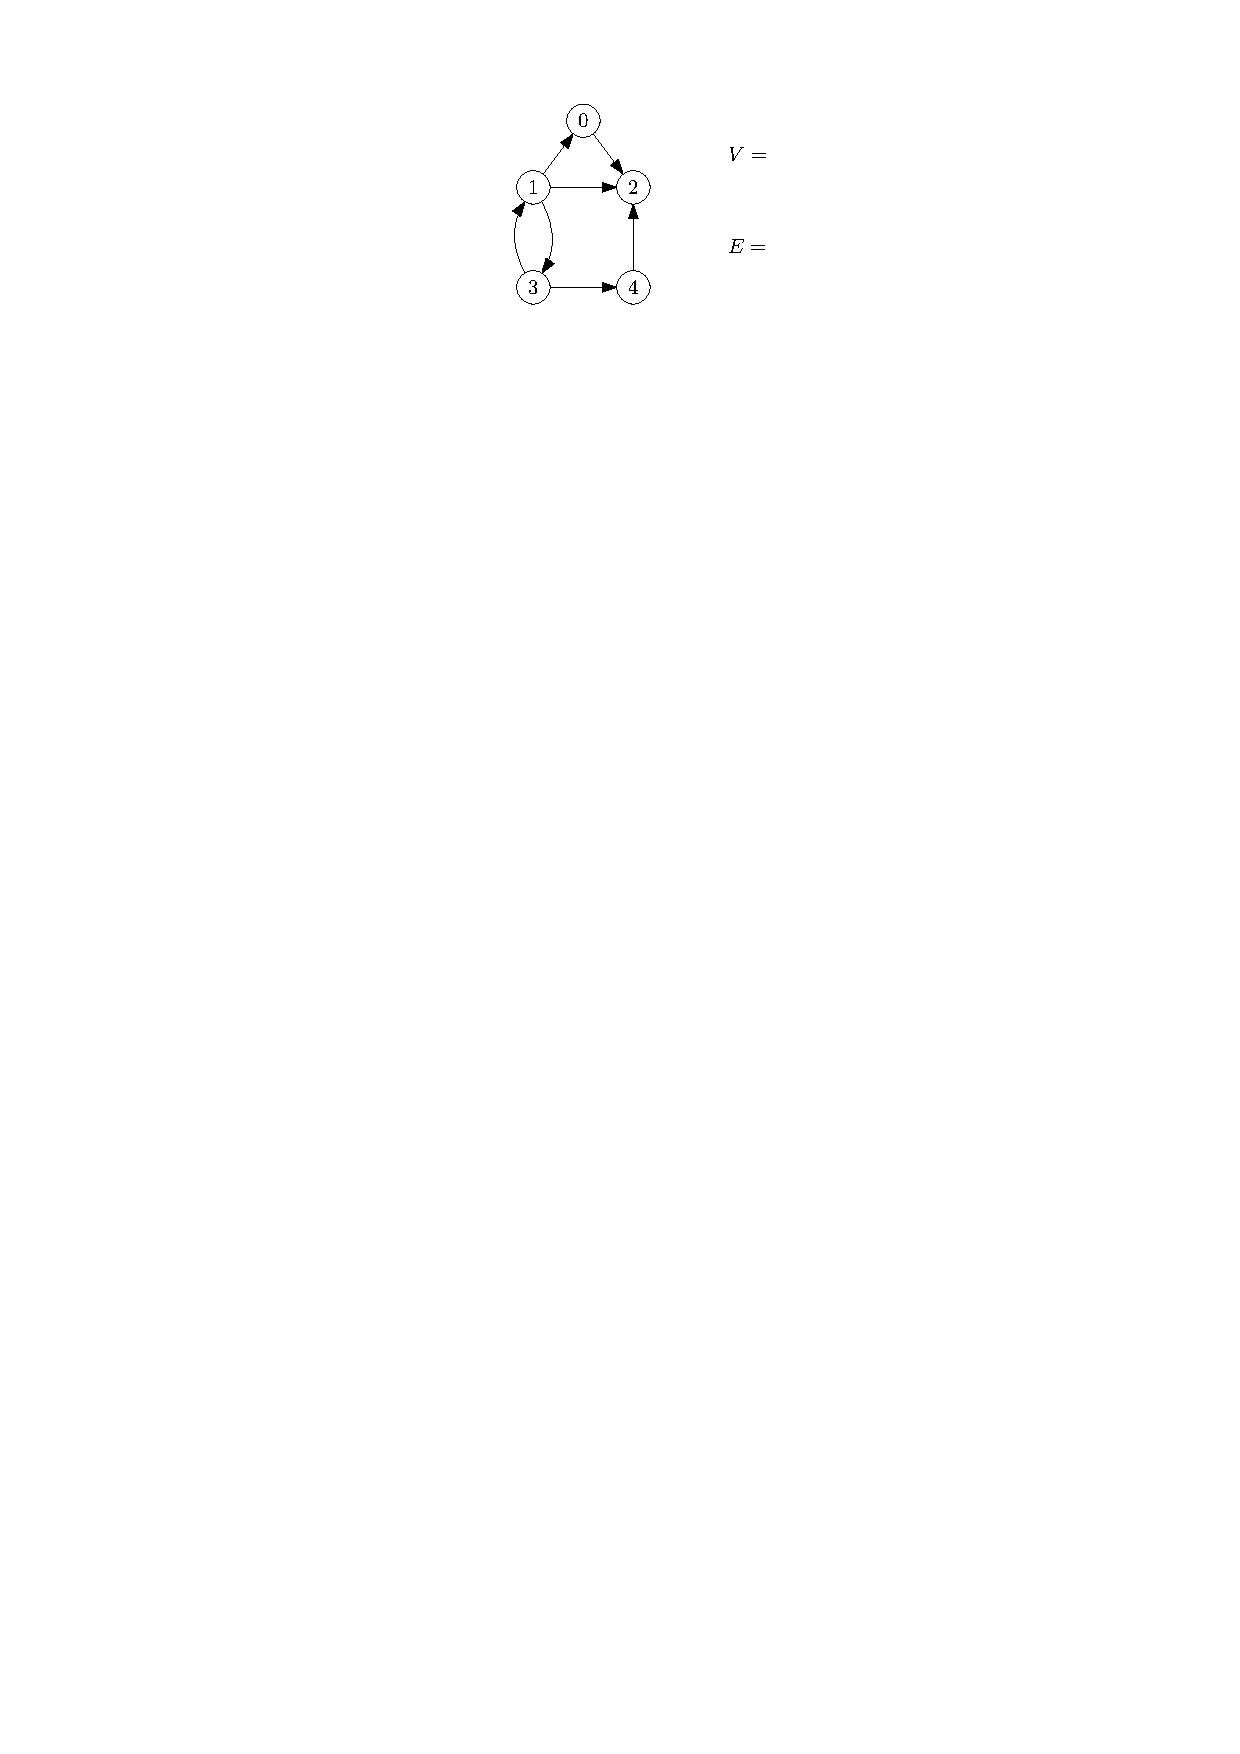
\includegraphics{graphExDirectedVE}
\end{Boxample}

\begin{Definition}\label{def:graph}
A \defnfont{graph} $G = (V, E)$ is a finite nonempty  set $V$ of 
\defnfont{vertices} together with a (possibly empty) set $E$ of unordered
pairs of vertices of $G$ called \defnfont{edges}. 
Note that the singular of vertices is \defnfont{vertex}.
\end{Definition}

\begin{Boxample}[0.5] \label{ex:graph}
For the graph shown, write down the sets $V$ and $E$.\\
\newline 
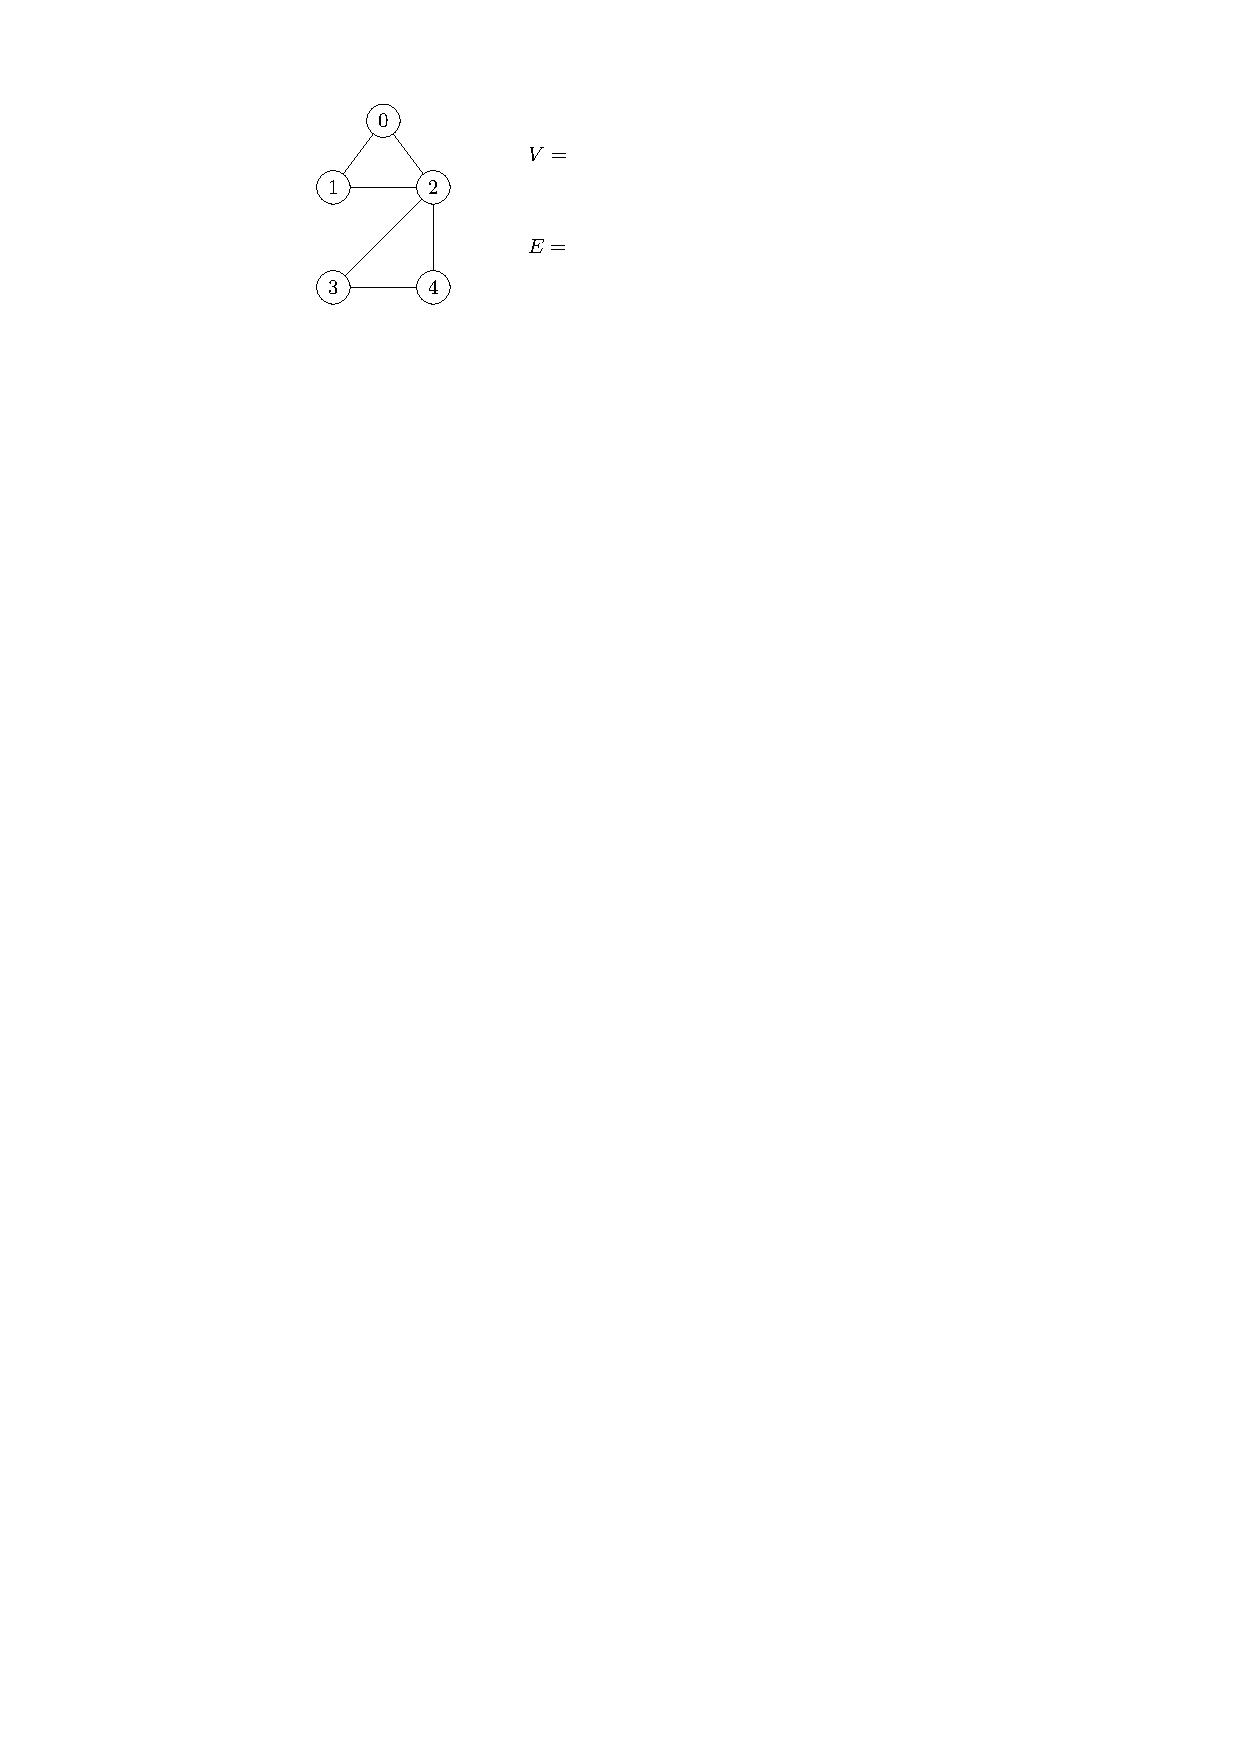
\includegraphics{graphExUndirectedVE}
\end{Boxample}

Some notes on graphs vs digraphs.
\begin{itemize}
  \item In order to save writing ``(di)graph" too many times, we treat the digraph as the fundamental concept.
  \item When we say something about digraphs, nodes and arcs, it is understood to also hold for graphs, 
  vertices and edges unless explicitly stated otherwise. 
  \item However, if we talk about graphs, vertices and edges, our statement is not necessarily true for digraphs. 
  \item Some authors use ``undirected graph'' to mean graph and use the term ``graph" to mean what we call a directed graph. 
  We always use digraph and graph.
  \item $E$ is a set so there are no multiple arcs between a pair of nodes.
  \item An arc that begins and ends at the same node is called a \defnfont{loop}. 
  We make the convention that \boldfont{loops are not allowed in our digraphs}. 
  \item For a digraph $G$ we may denote the node set $V(G)$ and arc set $E(G)$ for clarity.
  \item A graph can be viewed as a digraph where every unordered edge $\{u, v\}$ 
  is replaced by two directed arcs $(u, v)$ and $(v, u)$.  
  This works in most instances and has the advantage of allowing us to consider only digraphs.
%  \item Sometimes we must know whether our object is really a graph or just a symmetric digraph. Whenever there
%  is a potential ambiguity, we shall point it out.
\end{itemize}

\begin{Definition}\label{def:adjacent}  
If $(u, v)\in E$ (that is, if there is an arc going from $u$ to $v$) we say that $v$ is \defnfont{adjacent} 
to $u$, that $v$ is an \defnfont{out-neighbour} of $u$, and that $u$ is an \defnfont{in-neighbour} of $v$.
In an (undirected) graph $G$, if $\{u, v\} \in E$, then $u$ is a \defnfont{neighbour} of $v$ and $v$ is a neighbour of $u$. 
\end{Definition}

\begin{Boxample}[2]
In the digraph in \cref{ex:digraph}, find all in-neighbours of node~2 and all out-neighbours of node 0.
\end{Boxample}

\begin{Definition} 
The \defnfont{order} of a digraph $G = (V, E)$ is $\abs{V}$, the number of nodes. 
The \defnfont{size} of $G$ is $\abs{E}$, the number of arcs. 
We usually use $n$ to denote $\abs{V}$ and $m$ to denote $\abs{E}$.
\end{Definition}
 
For a given order $n$, the size $m$ can be as low as $0$ (a digraph consisting of $n$ nodes and no arcs)  
and as high as $n(n-1)$ (each node can point to each other node; recall that we do not allow loops).

\begin{Definition}  
If $m$ is toward the low end, the digraph is called \defnfont{sparse}, 
and if $m$ is toward the high end, then the digraph is called \defnfont{dense}. 
These terms are obviously very informal. 
For our purposes we will call a class of digraphs sparse if $m$ is $O(n)$ and dense if $m$ is $\Omega(n^2)$.
\end{Definition}

\begin{Definition} 
A \defnfont{walk} in a digraph $G$ is a sequence of nodes $v_0\, v_1\, \ldots\, v_l$ 
such that, for each $i$ with $0 \leq i < l$, $(v_i, v_{i+1})$ is an arc in $G$. 

The \defnfont{length} of the walk $v_0\, v_1\, \ldots \,v_l$ is the number $l$ (that is, the number of arcs involved).

A \defnfont{path} is a walk in which no node is repeated. 

A \defnfont{cycle} is a walk in which $v_0 = v_l$ and no other nodes
are repeated.
\end{Definition}

In a graph, a walk of the form $u\, v\, u$ -- going back and forth along the same edge -- is not considered a cycle. 
A cycle in a graph must be of length at least $3$.
Note that a walk and a path can have length 0.


\begin{Boxample}
For the graph on the left the following
sequences of vertices are classified as being walks, paths, or cycles. Complete the table.\\

\begin{minipage}[c]{0.3\textwidth}
\centering
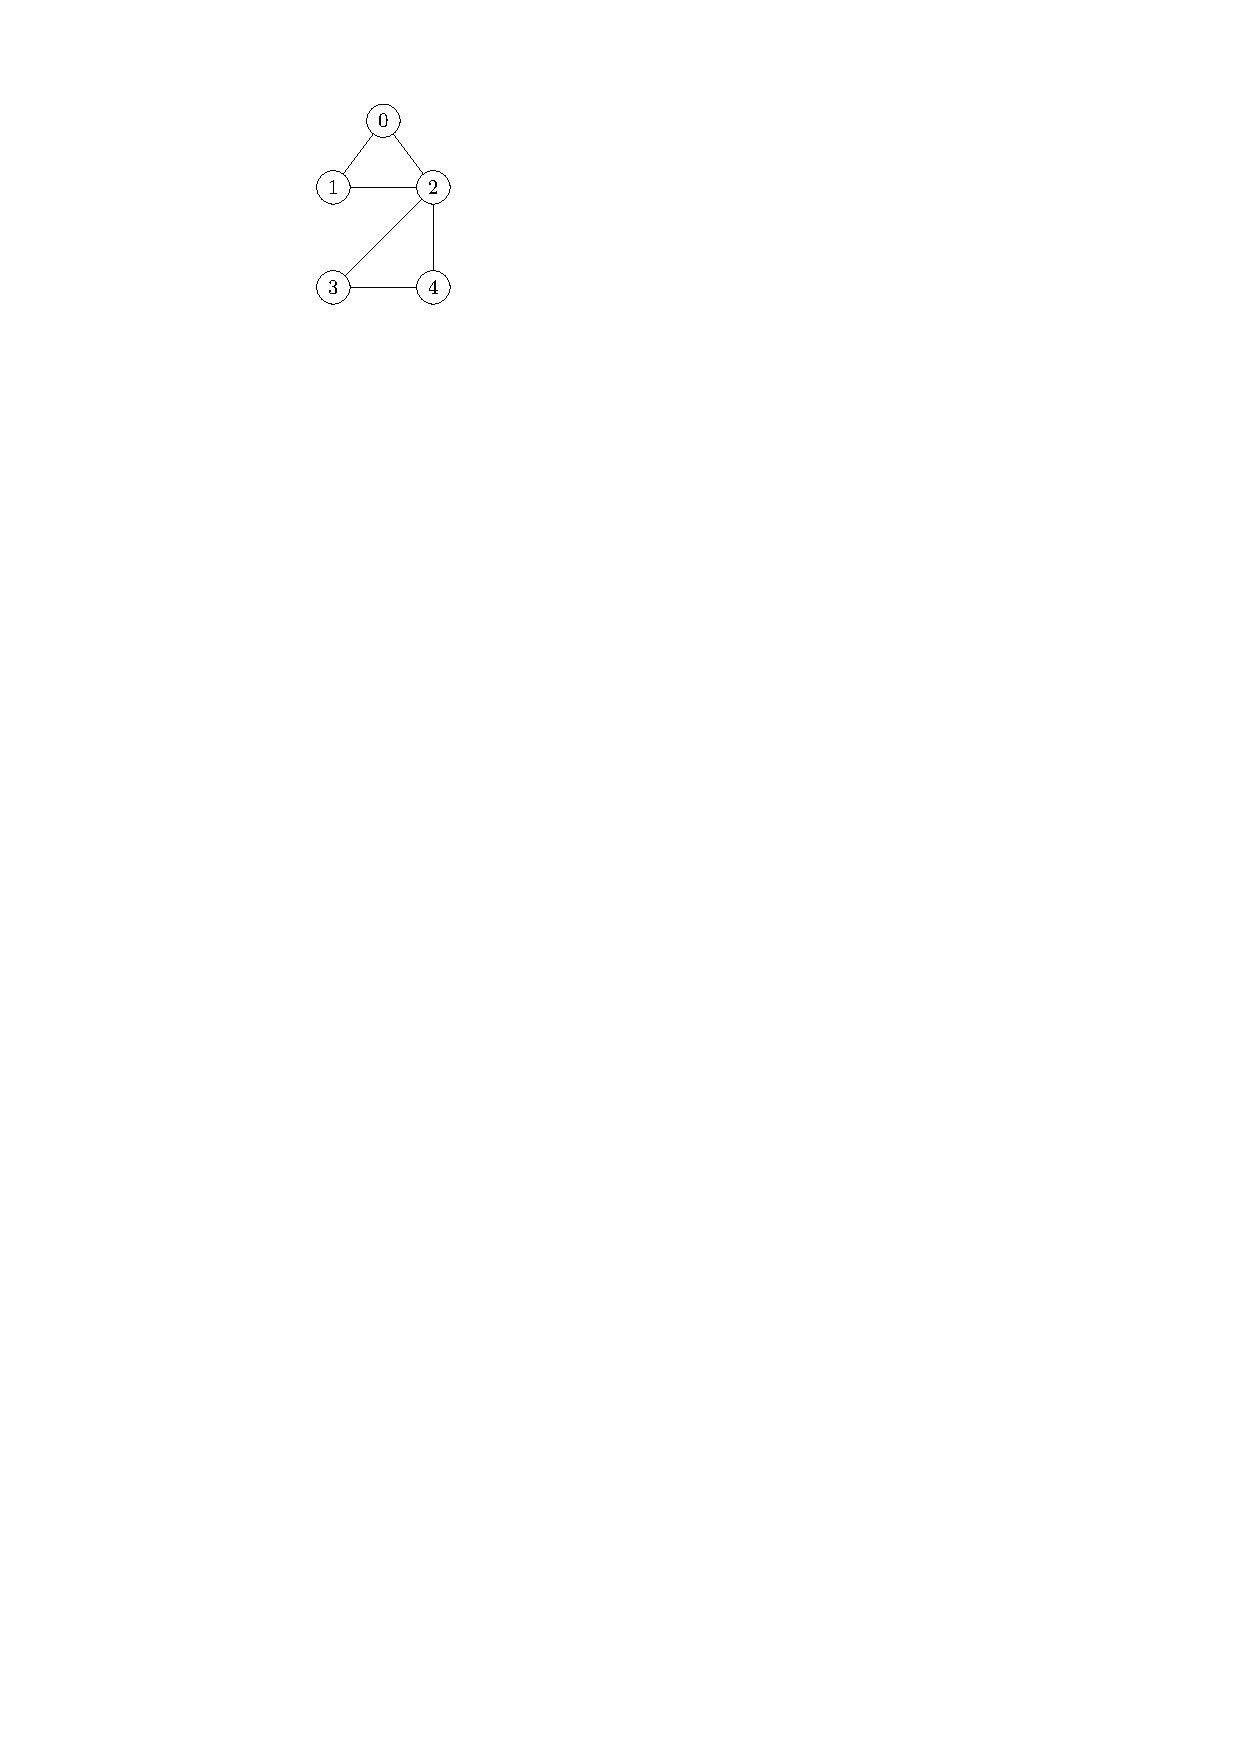
\includegraphics{graphExUndirected}
\end{minipage}
\begin{minipage}[c]{0.65\textwidth}
\begin{tabular}{|l|c|c|c|}\hline
\textbf{vertex sequence} & \textbf{walk?} & \textbf{path?} & \textbf{cycle?} \\ \hline
$0\, 3\, 2$                  & no  & no  &   \\
$0\, 1\, 2\, 3\, 4$          &     & yes & no  \\
$0\, 1\,  2\,  0$            & yes &     & yes  \\
$0 \, 1\,  0$                & yes & no  &  \\
$1\,  2\,  3\,  4\,  2\,  0$ &     &     &  \\
$3$							 & yes &     &  \\
\hline
\end{tabular}
\end{minipage}
\end{Boxample}

\begin{Boxample}[7]
Show that if there is a walk from $u$ to $v$, then we can find a path from $u$ to $v$.
\end{Boxample}

\begin{Definition} 
In a graph, the \defnfont{degree} of a vertex $v$ is the number of edges meeting $v$. 
In a digraph, the \defnfont{outdegree} of a node $v$ is the number of out-neighbours of $v$, 
and the \defnfont{indegree} of $v$ is the number of in-neighbours of $v$.

A node of indegree $0$ is called a \defnfont{source} and a node of outdegree $0$ is called a \defnfont{sink}.
\end{Definition}

%\begin{Boxample}[3]
%Prove that in a digraph, the sum of all outdegrees equals the sum of all 
%indegrees. What is the analogous statement for a graph? 
%\end{Boxample}

\begin{Definition}
The \defnfont{distance} from $u$ to $v$ in $G$, denoted by $d(u,v)$, is 
the number of arc on a shortest path from $u$ to $v$. If no path from $u$ to $v$ exists, the 
distance is undefined (or $+\infty$).
\end{Definition}

For graphs, we have $d(u,v) = d(v,u)$ for all vertices $u, v$. 

\begin{Boxample}[2]
Give the following distances for the digraph on the left.\\
\newline
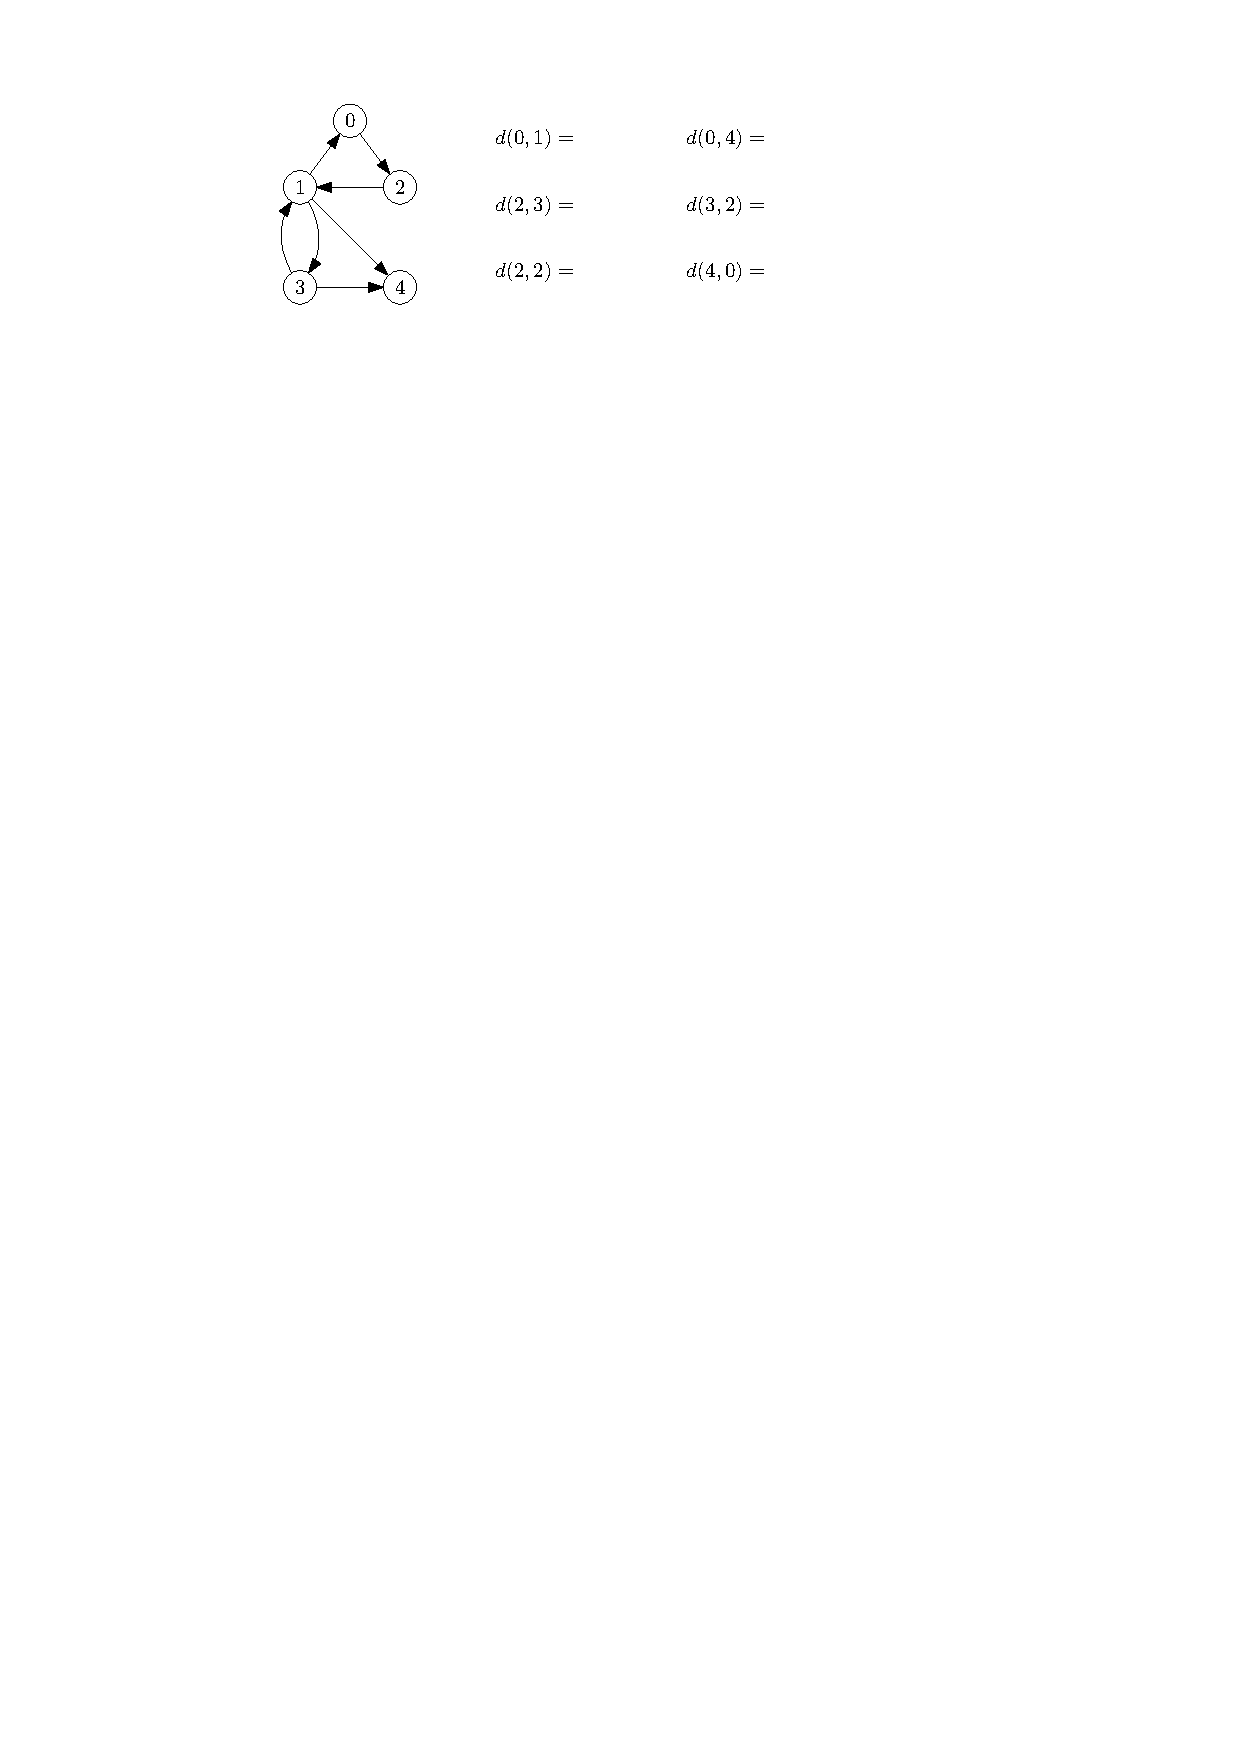
\includegraphics{distancesDirected}
\newline

Why are the values $d(4, v)$ not defined unless $v = 4$?
\end{Boxample}

\section{Creating new digraphs from old ones}
There are several ways to create new digraphs from old ones.
One way is to delete nodes and arcs in such a way that the 
resulting object is still a digraph (no arcs missing endpoints).

\begin{Definition}
A \defnfont{subdigraph} of a digraph $G = (V, E)$ is a digraph $G' = (V', E')$ 
where $V'\subseteq V$ and $E'\subseteq E$. 
A \defnfont{spanning} subdigraph is one with $V' = V$; that is, it contains all nodes.
\end{Definition}

\begin{Boxample}
A digraph (left) with a subdigraph (middle) and a spanning subdigraph (right).
\begin{center}
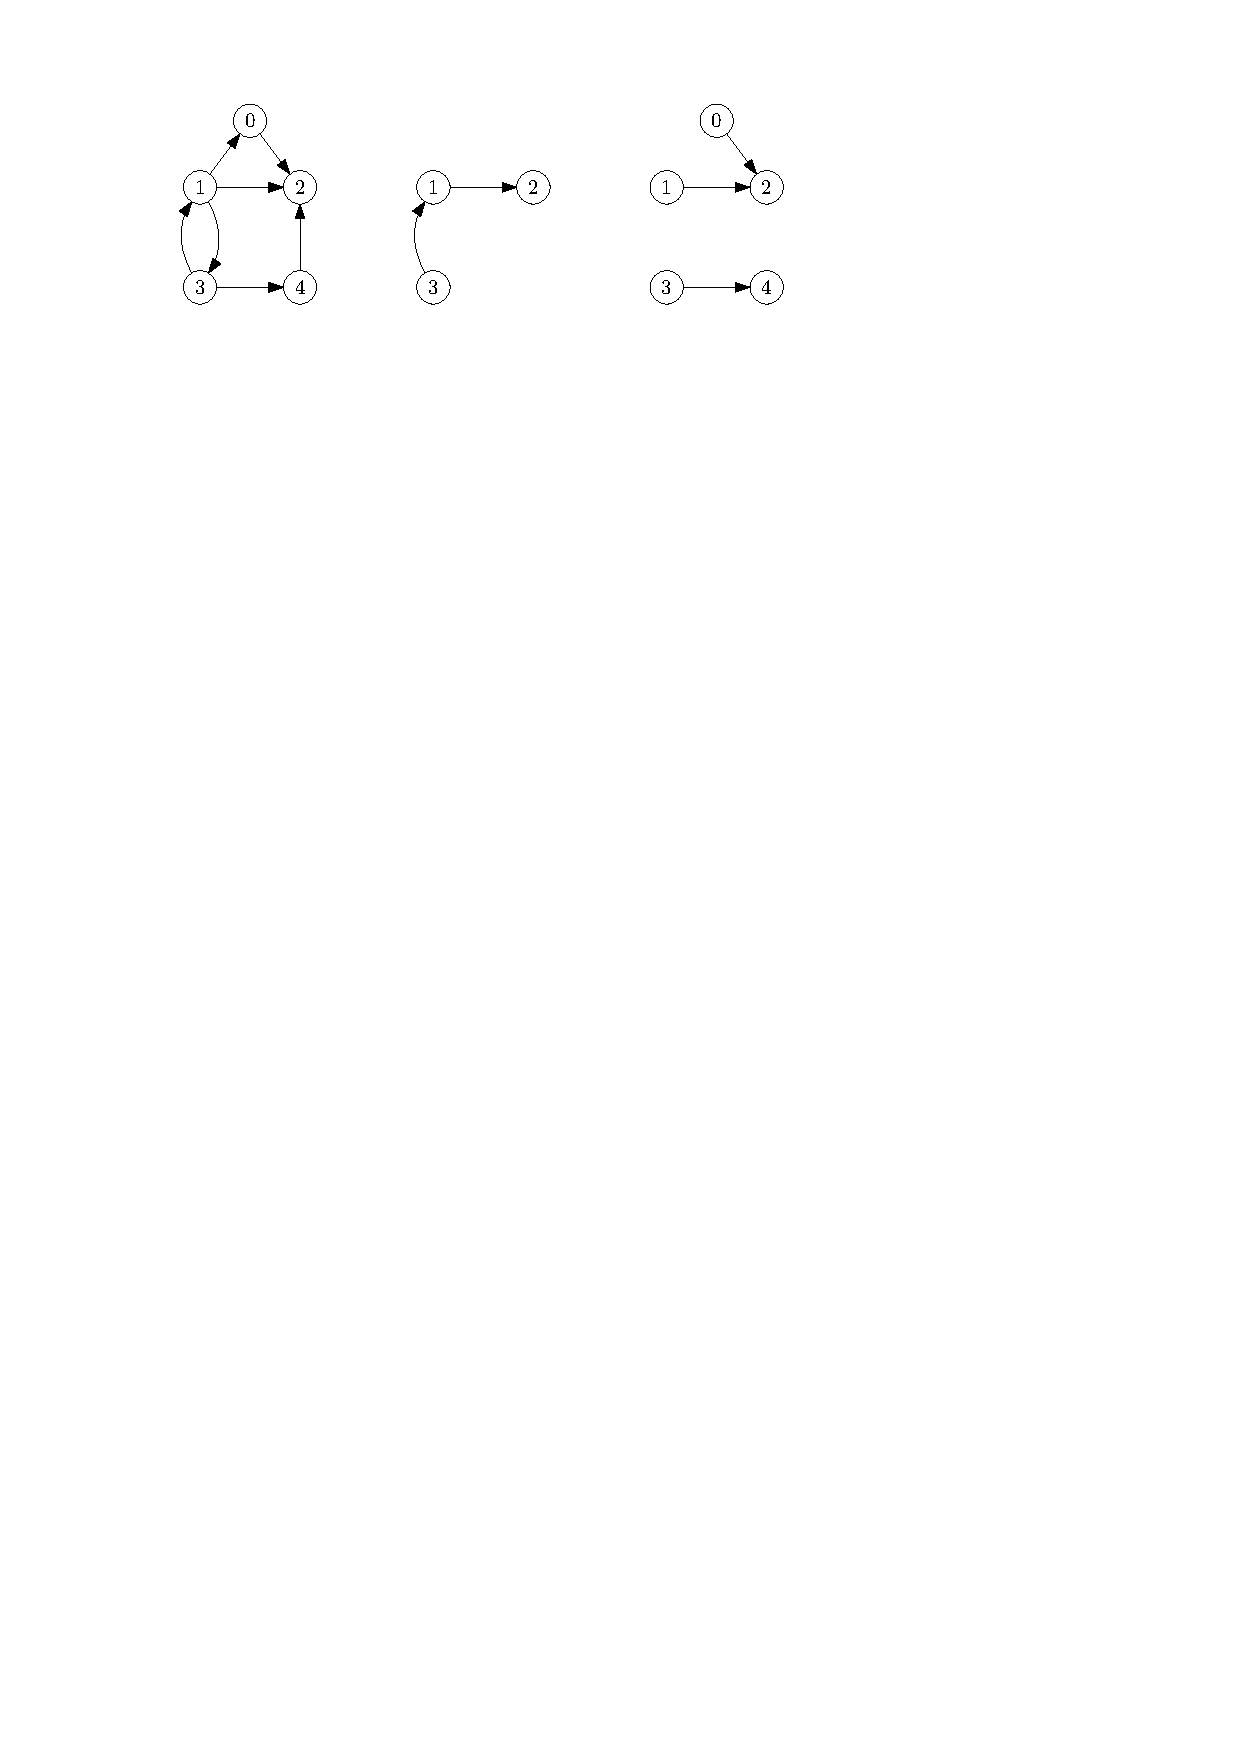
\includegraphics{graphExSubSpan} 
\end{center}
\end{Boxample}

\begin{Definition}
The subdigraph \defnfont{induced} by a subset $V'$ of $V$ is the digraph
$G' = (V', E')$ where $E' = \set{(u, v) \in E \mid u \in V' \mbox{ and } v\in V'}$.
\end{Definition}

\begin{Boxample}
For the digraph shown on the left, draw the subdigraph induced by  \set{1, 2, 3} on the right.
\begin{center}
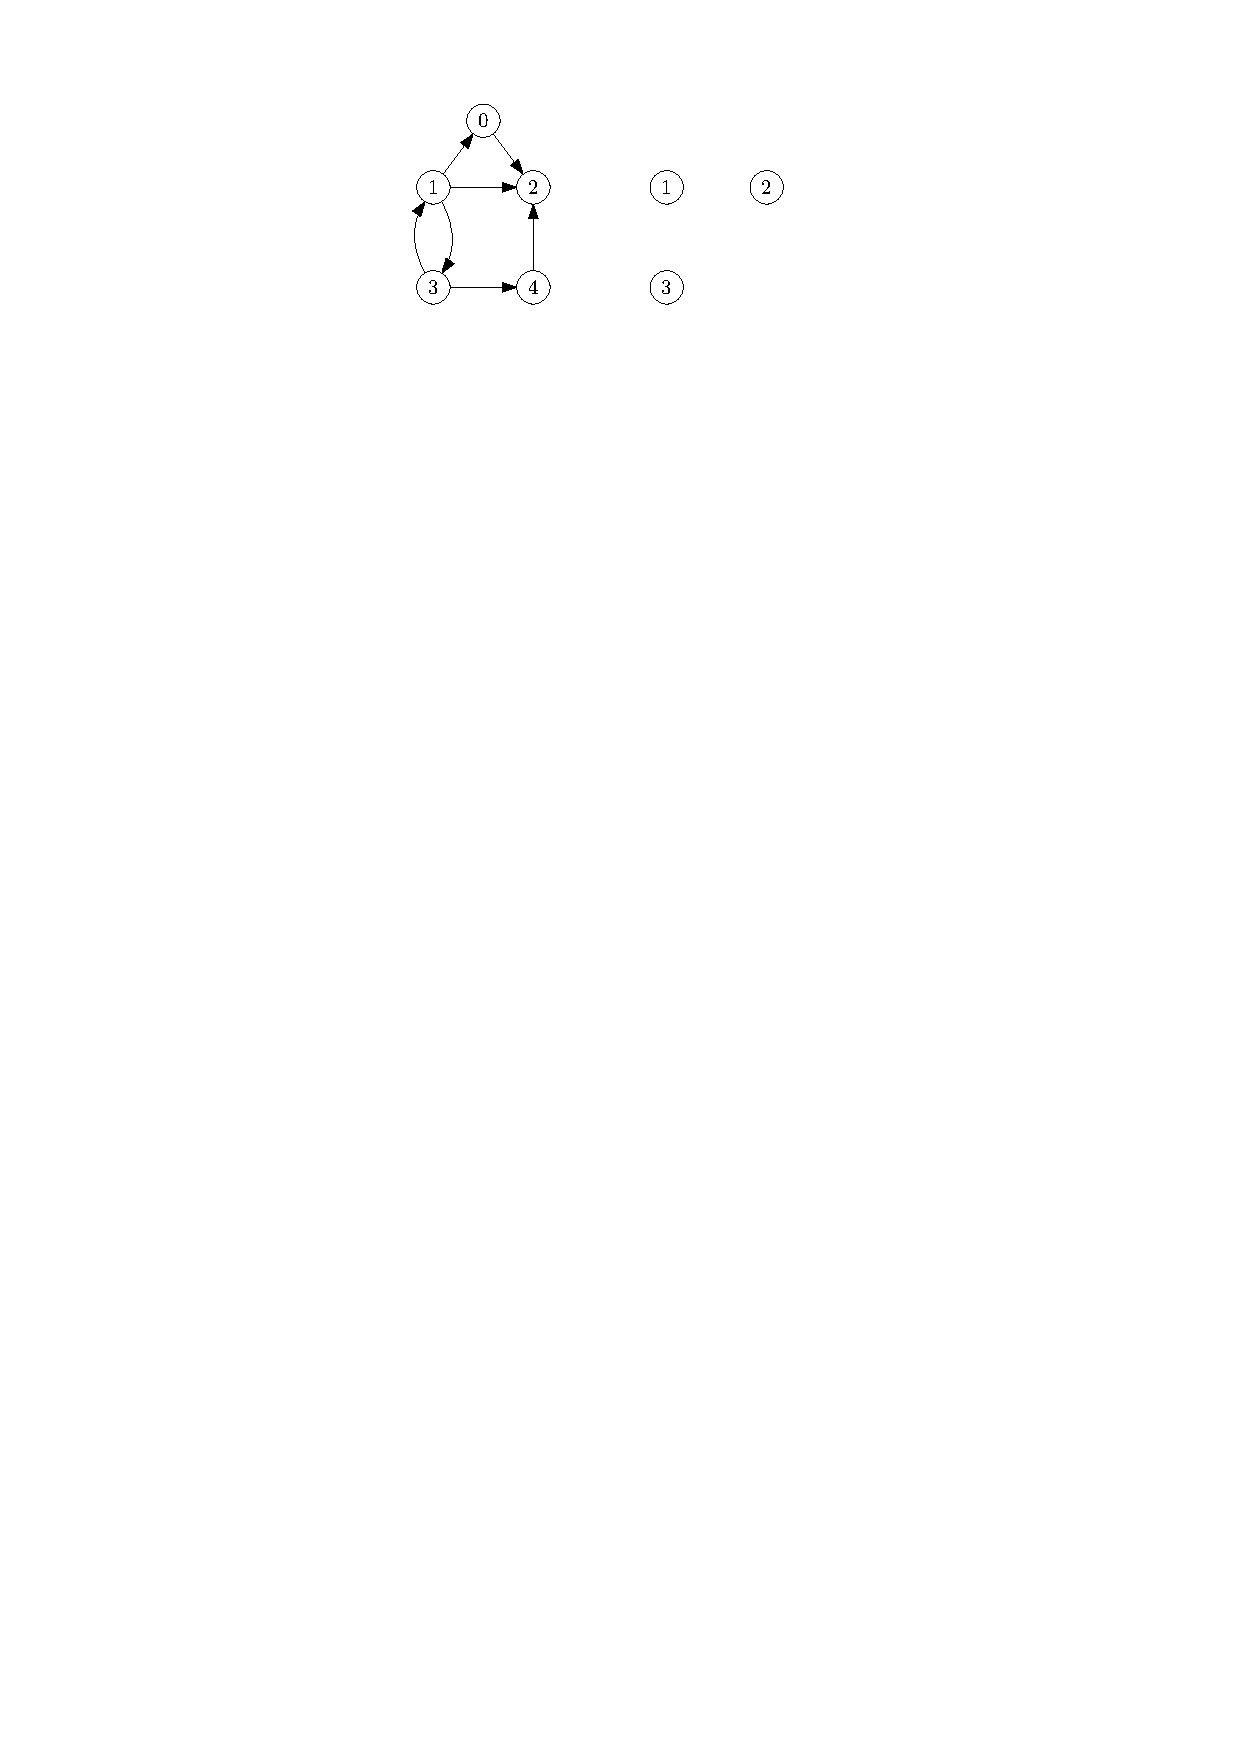
\includegraphics{graphExInducedEx}
\end{center}
\end{Boxample}

\begin{Definition}
The \defnfont{reverse digraph} of the digraph $G = (V, E)$, is the digraph $G_r = (V, E')$ where $(u, v)\in E'$ if and only if $(v, u)\in E$.
\end{Definition}

\begin{Boxample}\label{exr:compute-reverse}
Digraph $G$ and its reverse $G_r$. We simply reverse all the arrows.
\begin{center}
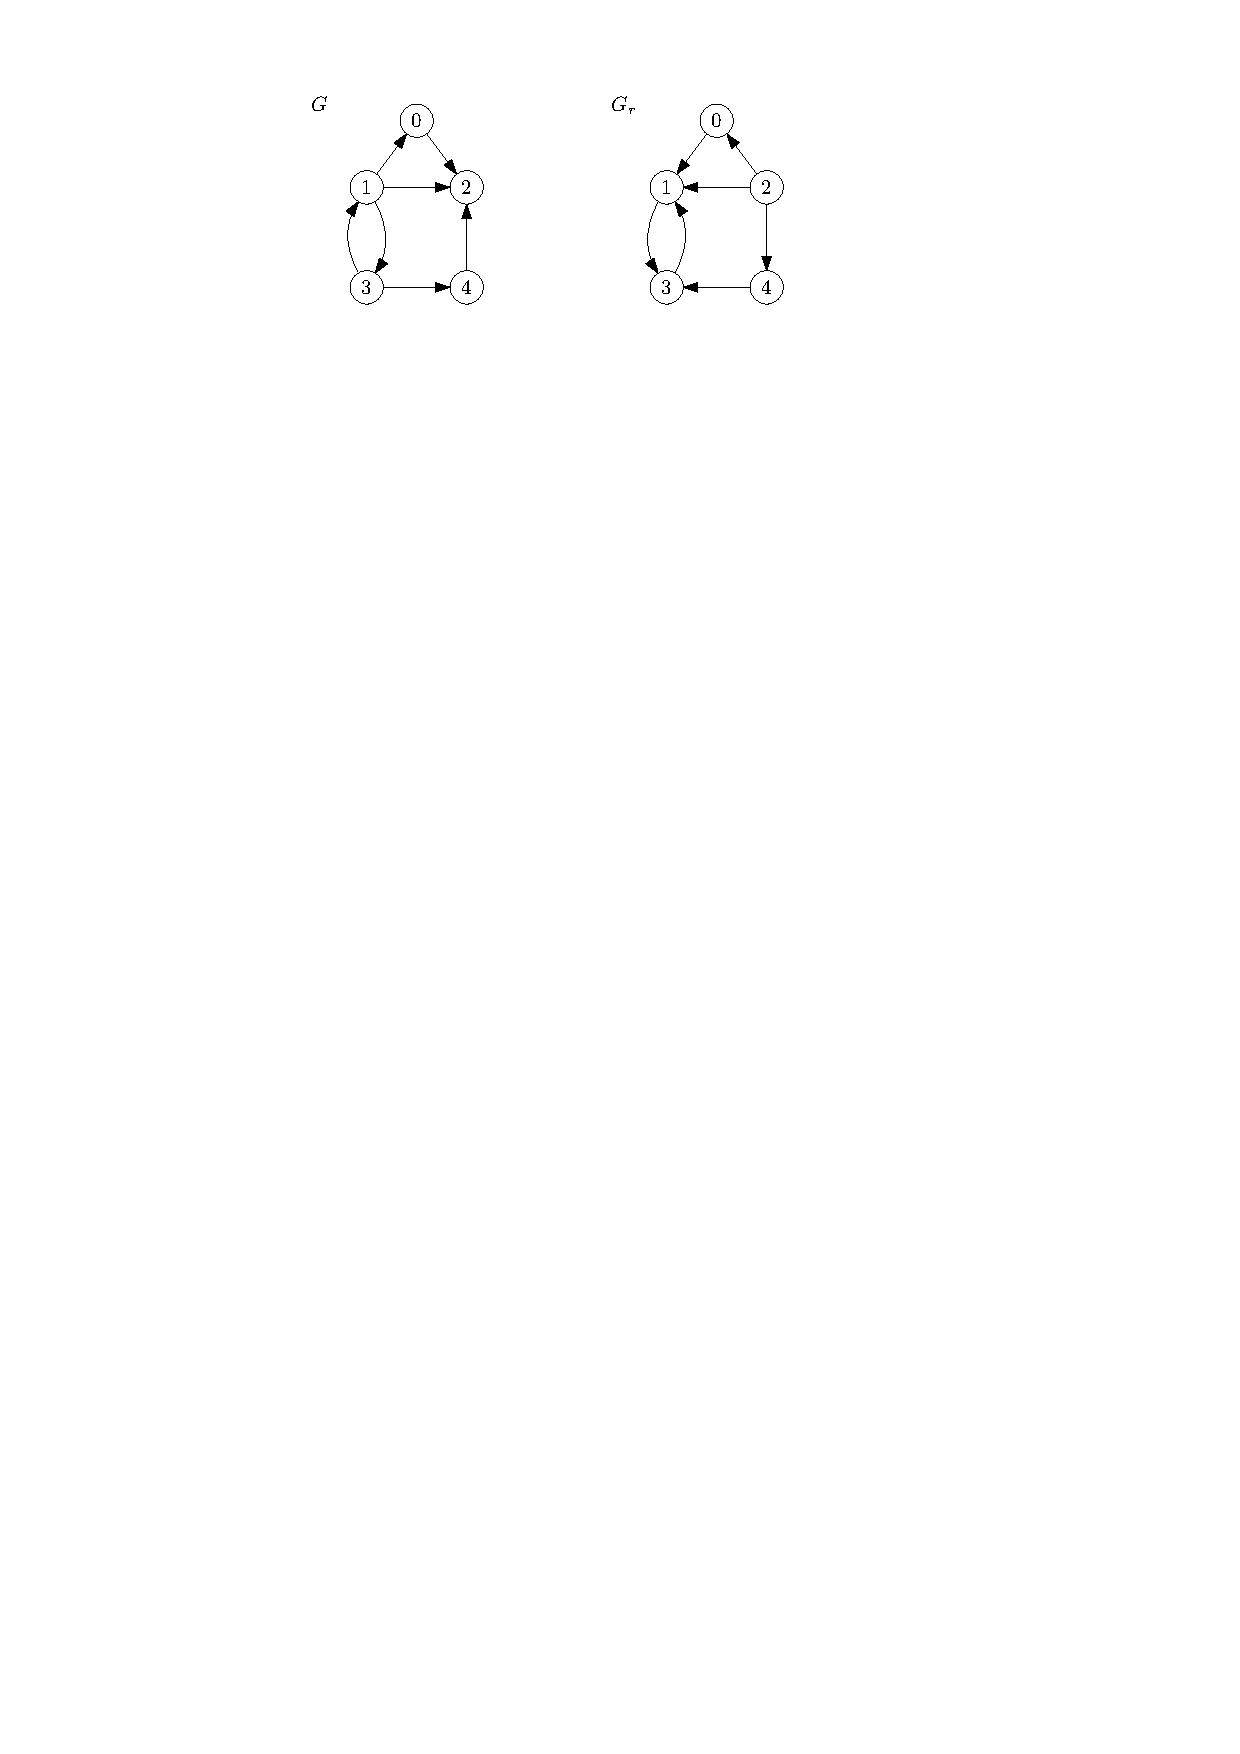
\includegraphics{graphExReverse}
\end{center}
\end{Boxample}

It is sometimes useful to ignore the direction of arcs in a digraph to find the associated `underlying graph'.

\begin{Definition} 
The \defnfont{underlying graph} of a digraph $G = (V, E)$ is the graph 
$G' = (V, E')$ where $E' = \set{\{u, v\} \mid (u, v)\in E}$.
\end{Definition}

Note that the underlying graph does not have multiple edges even when there are arcs $(u, v)$ and $(v, u)$. 
In that case, only one edge joins $u$ and $v$ in the underlying graph $G'$.  
%This is because $\{u, v\}$ and $\{v, u\}$ are equal as sets, so appear only once in the set $E'$.

\begin{Boxample}
Draw the underlying graph $G'$ of the digraph $G$.
\begin{center}
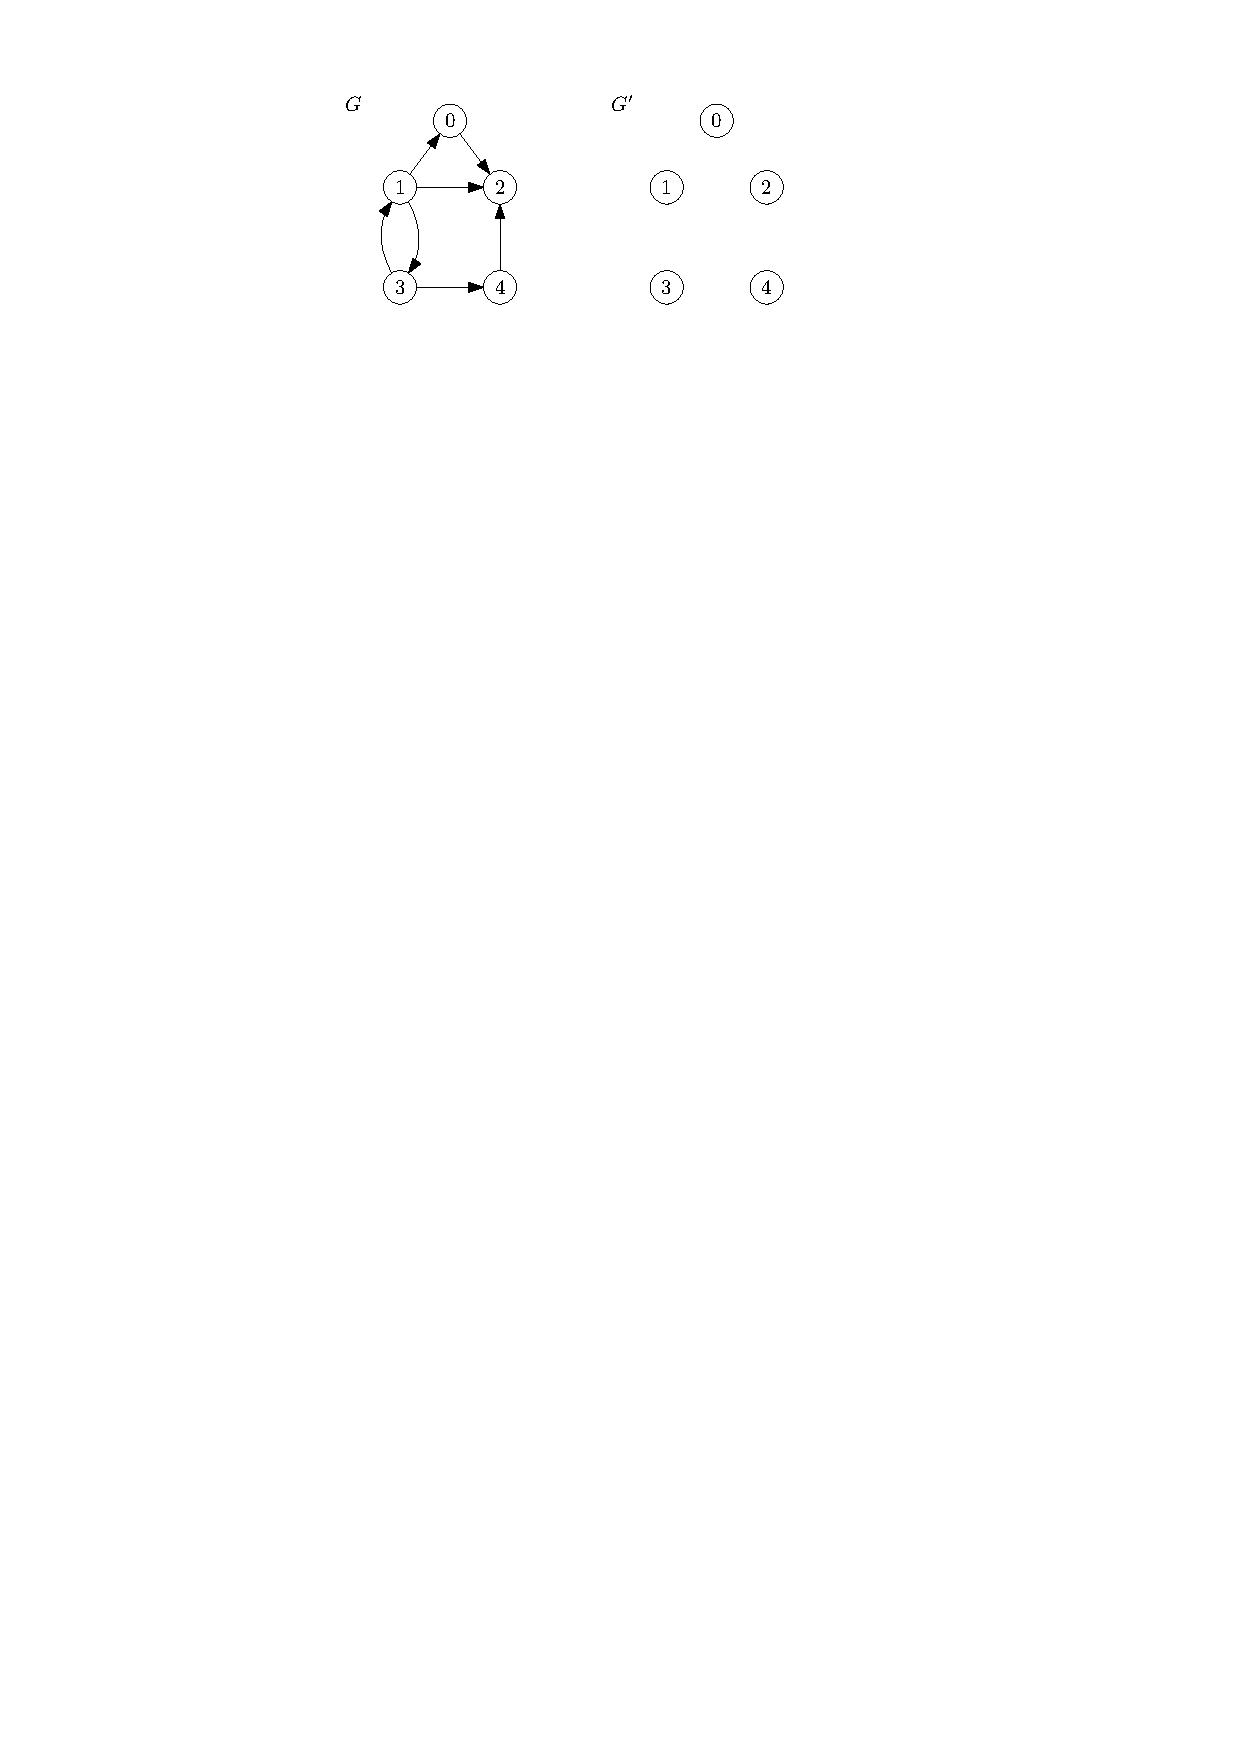
\includegraphics{graphExUnderlyingEx}
\end{center}
%Note that there should be only a single edge between vertices 1 and 3.
\end{Boxample}

\begin{Definition} 
We can combine two or more digraphs $G_1, G_2$, \ldots $G_k$ into a
single graph where the vertices of each $G_i$ are completely disjoint from
each other and no arc goes between the different $G_i$. The constructed
graph $G$ is called the \defnfont{graph union}, where $V(G) = V(G_1) \cup
V(G_2) \cup \ldots \cup V(G_k)$ and $E(G) = E(G_1) \cup E(G_2) \cup \ldots
\cup E(G_k)$.
\end{Definition}

%\begin{Boxample}[3] \label{ex:distbound}
%Let $G$ be a digraph of order $n$ and $u, v$ nodes of $G$. 
%Show that $d(u, v) \leq n - 1$ if there is a walk from $u$ to $v$.
%\end{Boxample}

%\begin{Boxample}[3] \label{ex:sparse-deg}
%Prove that in a sparse digraph, the average indegree of a node is $O(1)$, 
% while in a dense digraph, the average indegree of a node is $\Omega(n)$.
%\end{Boxample}

 

\chapter{Graph data structures} \label{sec:graph-reps} %---------------------------------
When representing a digraph in a computer, we assume
that it has nodes given in a fixed order with the
\boldfont{convention that the nodes are labelled $0, 1, \dots, n - 1$}.

\begin{Definition}
Let $G$ be a digraph of order $n$. The \defnfont{adjacency matrix} of $G$
is the $n\times n$ Boolean matrix (often encoded with $0$'s and $1$'s)
such that entry $(i, j)$ is true if and only if there is an arc from the
node $i$ to node $j$.
\end{Definition}

\begin{Definition}
For a digraph $G$ of order $n$, an \defnfont{adjacency lists}
representation is a sequence of $n$ sequences, $L_0, \dots, L_{n-1}$. 
Sequence $L_i$ contains all nodes of $G$ that are out-neighbours of node $i$.
\end{Definition}

%In the adjacency lists representation, only the out-neighbours of node $i$ are listed in the sequence $L_i$. 
In the adjacency lists representation, $L_i$ may or may not be sorted in order of increasing node number. 
Our \boldfont{convention is to sort them whenever convenient}. 
Many implementations do \boldfont{not} enforce this convention.

\begin{Boxample}
A graph and its adjacency matrix and adjacency list.\\
\begin{center}
\begin{minipage}[c]{0.3\textwidth}
\centering
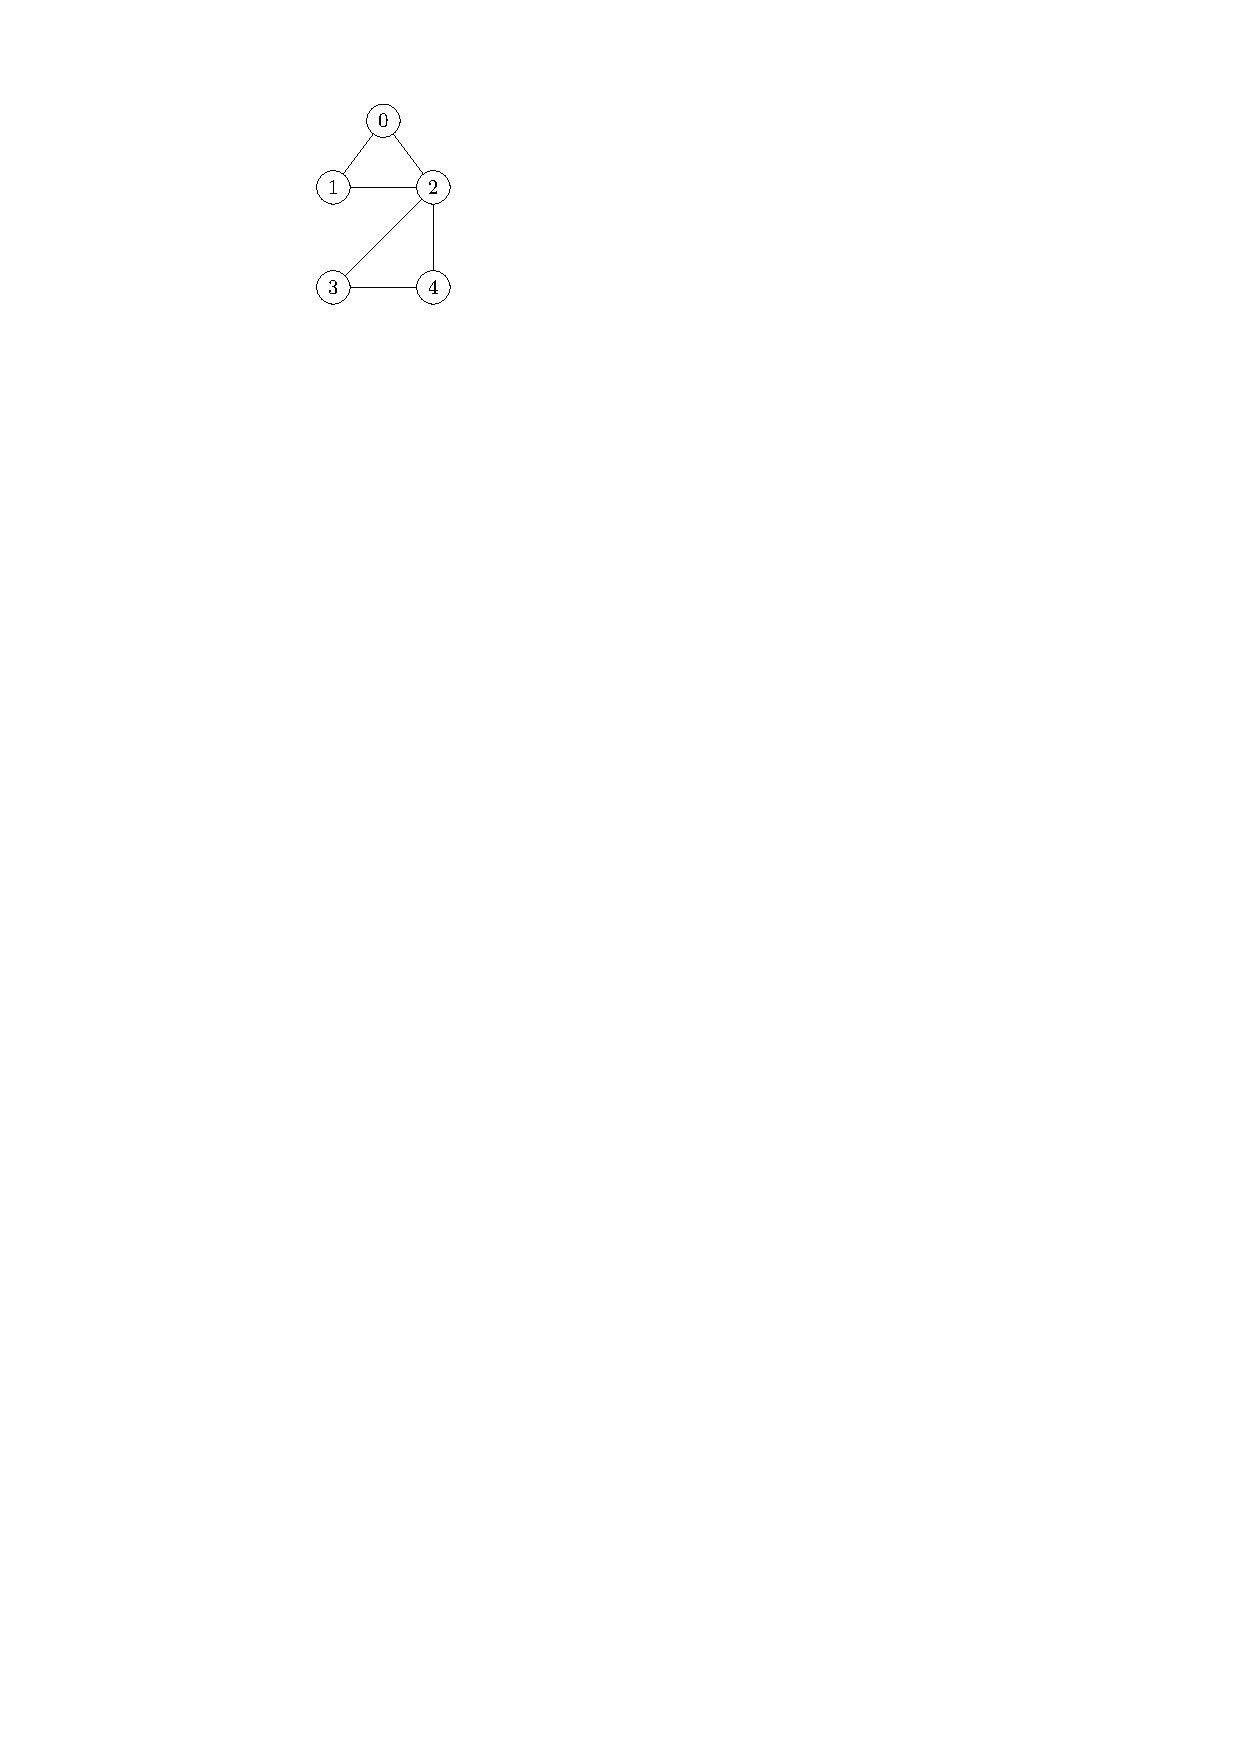
\includegraphics{graphExUndirected}
\end{minipage}
\begin{minipage}[c]{0.65\textwidth}
$\quad \left[
	\begin{matrix}
	0 & 1 & 1 & 0 & 0 \\
	1 & 0 & 1 & 0 & 0 \\
	1 & 1 & 0 & 1 & 1 \\
	0 & 0 & 1 & 0 & 1 \\
	0 & 0 & 1 & 1 & 0 
	\end{matrix}
\right] 
\qquad \qquad
\lightgraybox{
	\begin{array}{c|cccc}
	0 & 1 & 2 &   &   \\
	1 & 0 & 2 &   &   \\
	2 & 0 & 1 & 3 & 4 \\
	3 & 2 & 4 &   &   \\
	4 & 2 & 3 &   &   \\
	\end{array}
}$
\end{minipage}
\end{center}
Notice that the number of $1$'s in a row in the adjacency matrix is the outdegree of the corresponding node, 
while the number of $1$'s in a column is the indegree.
\end{Boxample}

\begin{Boxample}
\label{ex:adjlist}
A digraph and its adjacency matrix and adjacency list.\\
\begin{center}
\begin{minipage}[c]{0.3\textwidth}
\centering
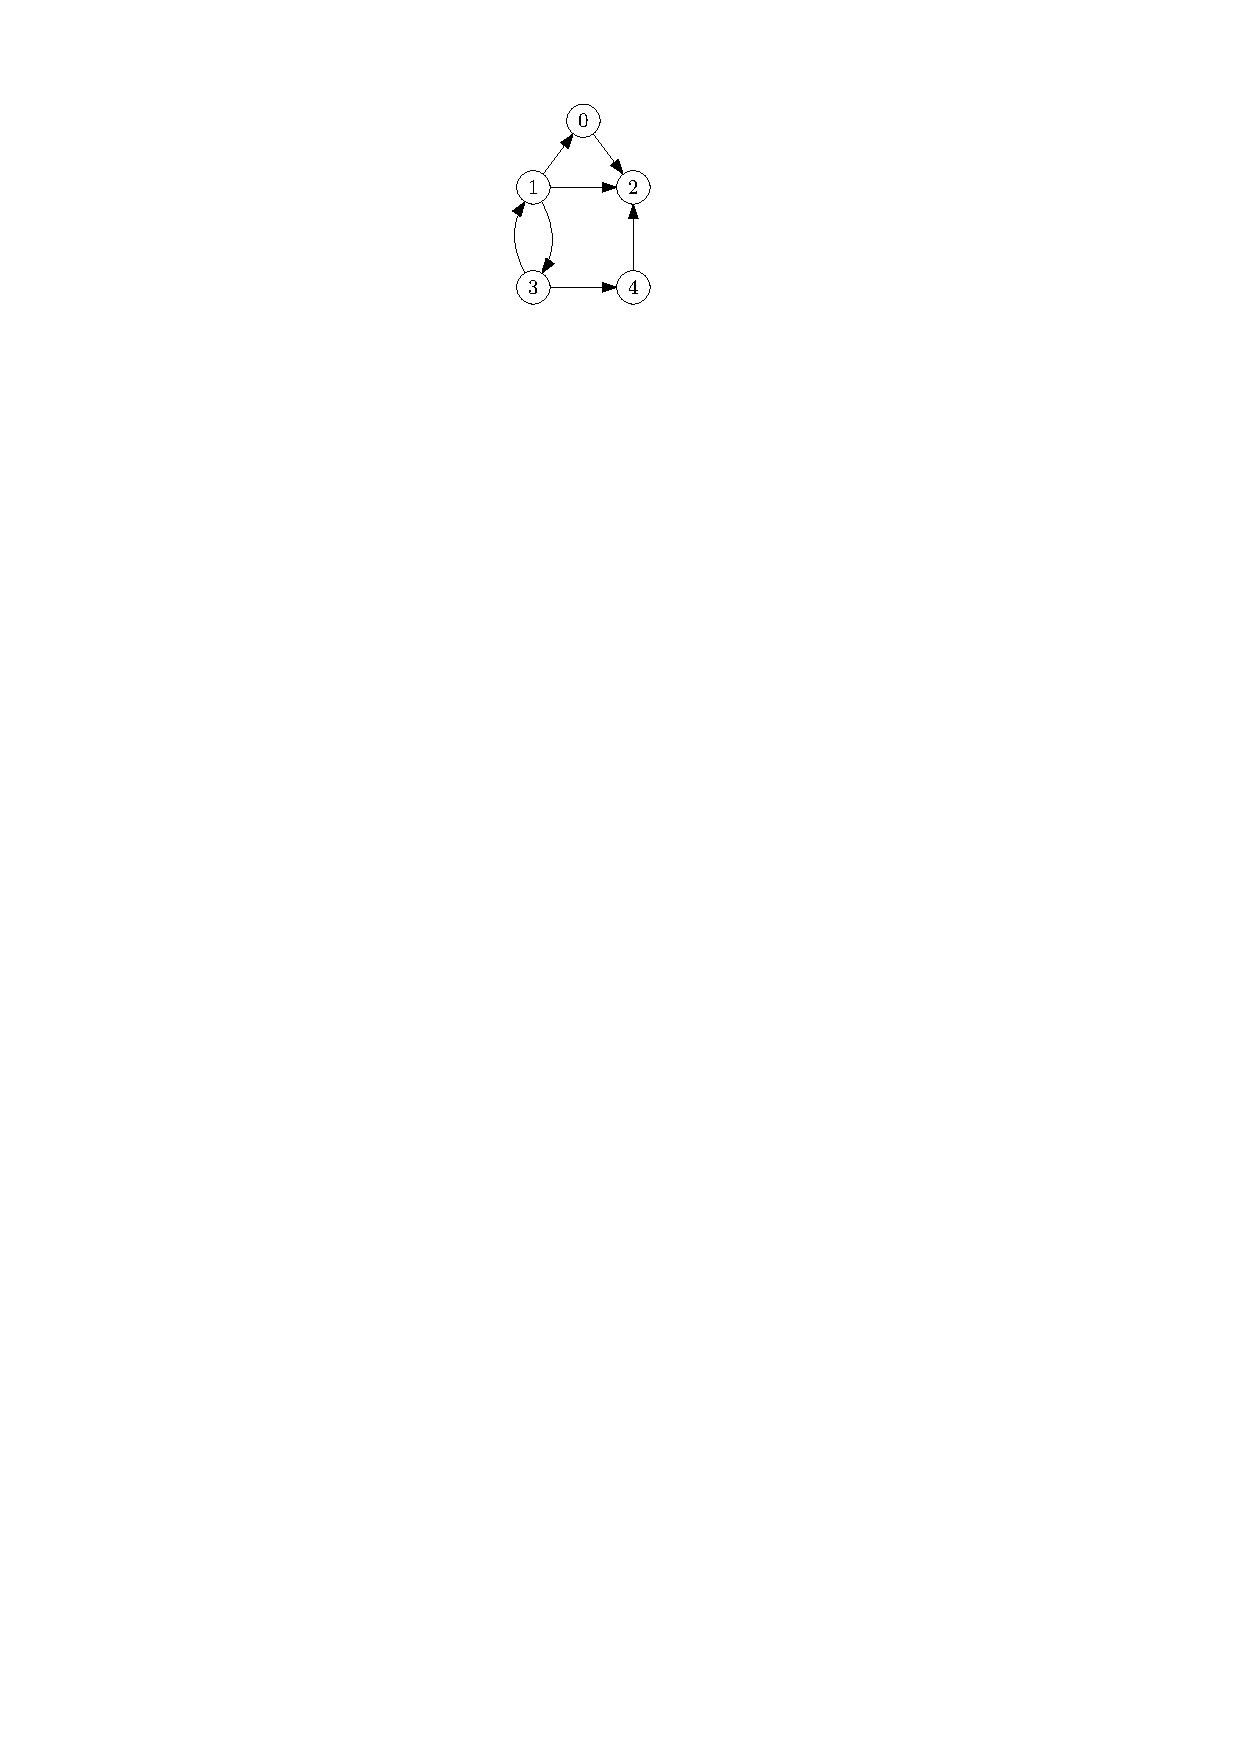
\includegraphics{graphExDirected}
\end{minipage}
\begin{minipage}[c]{0.65\textwidth}
$\quad\left[
	\begin{matrix}
	0 & 0 & 1 & 0 & 0 \\
	1 & 0 & 1 & 1 & 0 \\
	0 & 0 & 0 & 0 & 0 \\
	0 & 1 & 0 & 0 & 1 \\
	0 & 0 & 1 & 0 & 0 
	\end{matrix}
\right]
\qquad \qquad
\lightgraybox{
	\begin{array}{c|ccc}
	0 & 2  \\
	1 & 0 & 2 & 3  \\
	2  \\
	3 & 1 & 4  \\
	4 & 2 \\
	\end{array}
}$
\end{minipage}
\end{center}
An empty sequence occurs in the adjacency list where a node has no out-neighbours (for example, sequence $2$). 
\end{Boxample}

Sometimes the node labels in adjacency lists are omitted, so the digraph in \cref{ex:adjlist} would be written as:
$$\lightgraybox{
	\begin{array}{ccc}
	2 &   &   \\
	0 & 2 & 3 \\
	  &   &   \\
	1 & 4 &   \\
	2 &   &   \\
	\end{array}
}$$

\begin{Boxample}[2]
Give the adjacency matrix of the digraph below.

	\vspace{1cm}
	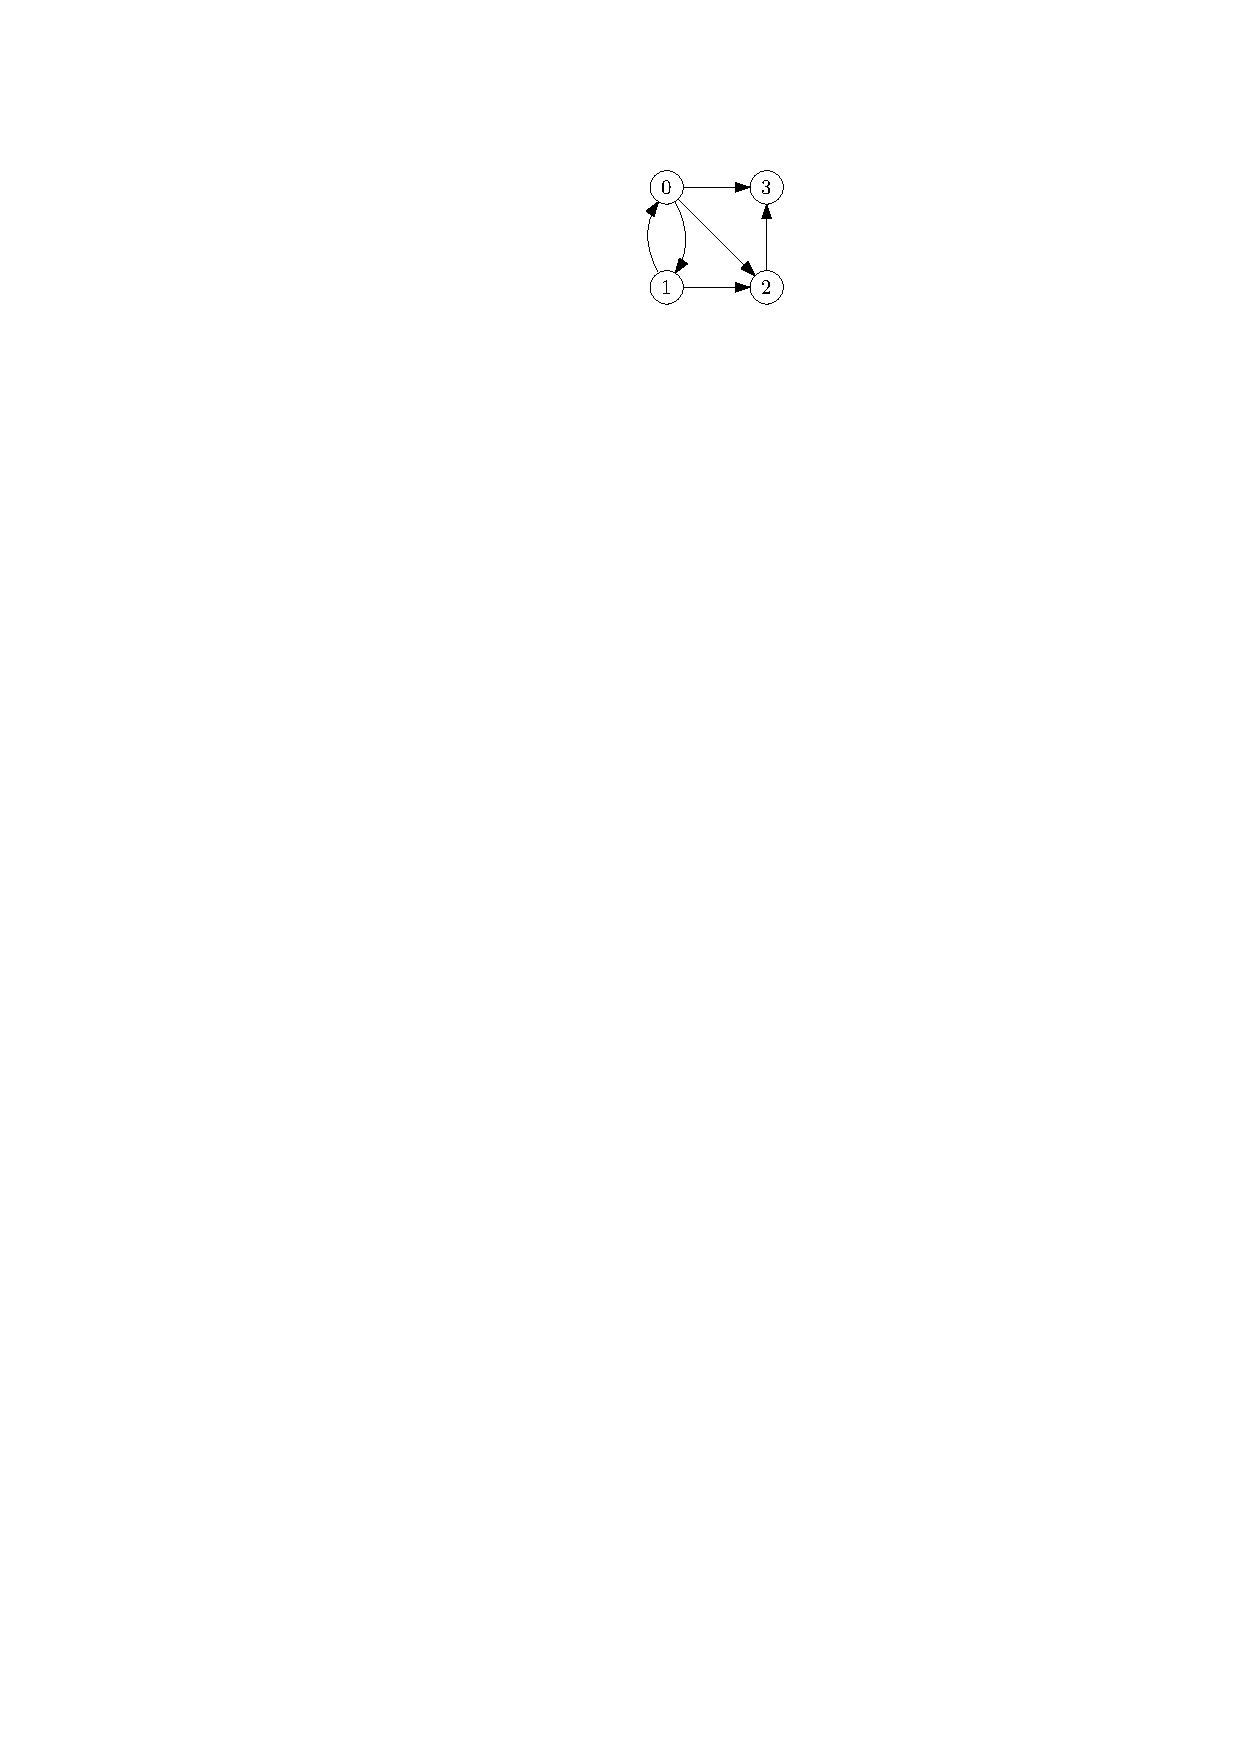
\includegraphics{graphEx4}
	\vspace{1cm}
	
Draw the digraph corresponding to the given adjacency matrix.

	\vspace{1cm}
	$\left[
	\begin{matrix}
	0 & 1 & 0 & 1 & 0 \\
	1 & 0 & 0 & 0 & 1 \\
	0 & 1 & 0 & 0 & 1 \\
	1 & 0 & 1 & 0 & 0 \\
	0 & 0 & 1 & 1 & 0 
	\end{matrix}
	\right]$
\end{Boxample}

\begin{Boxample}[1] \label{ex:drawadjlist}
Give the adjacency lists of the digraph below.

	\vspace{1cm}
	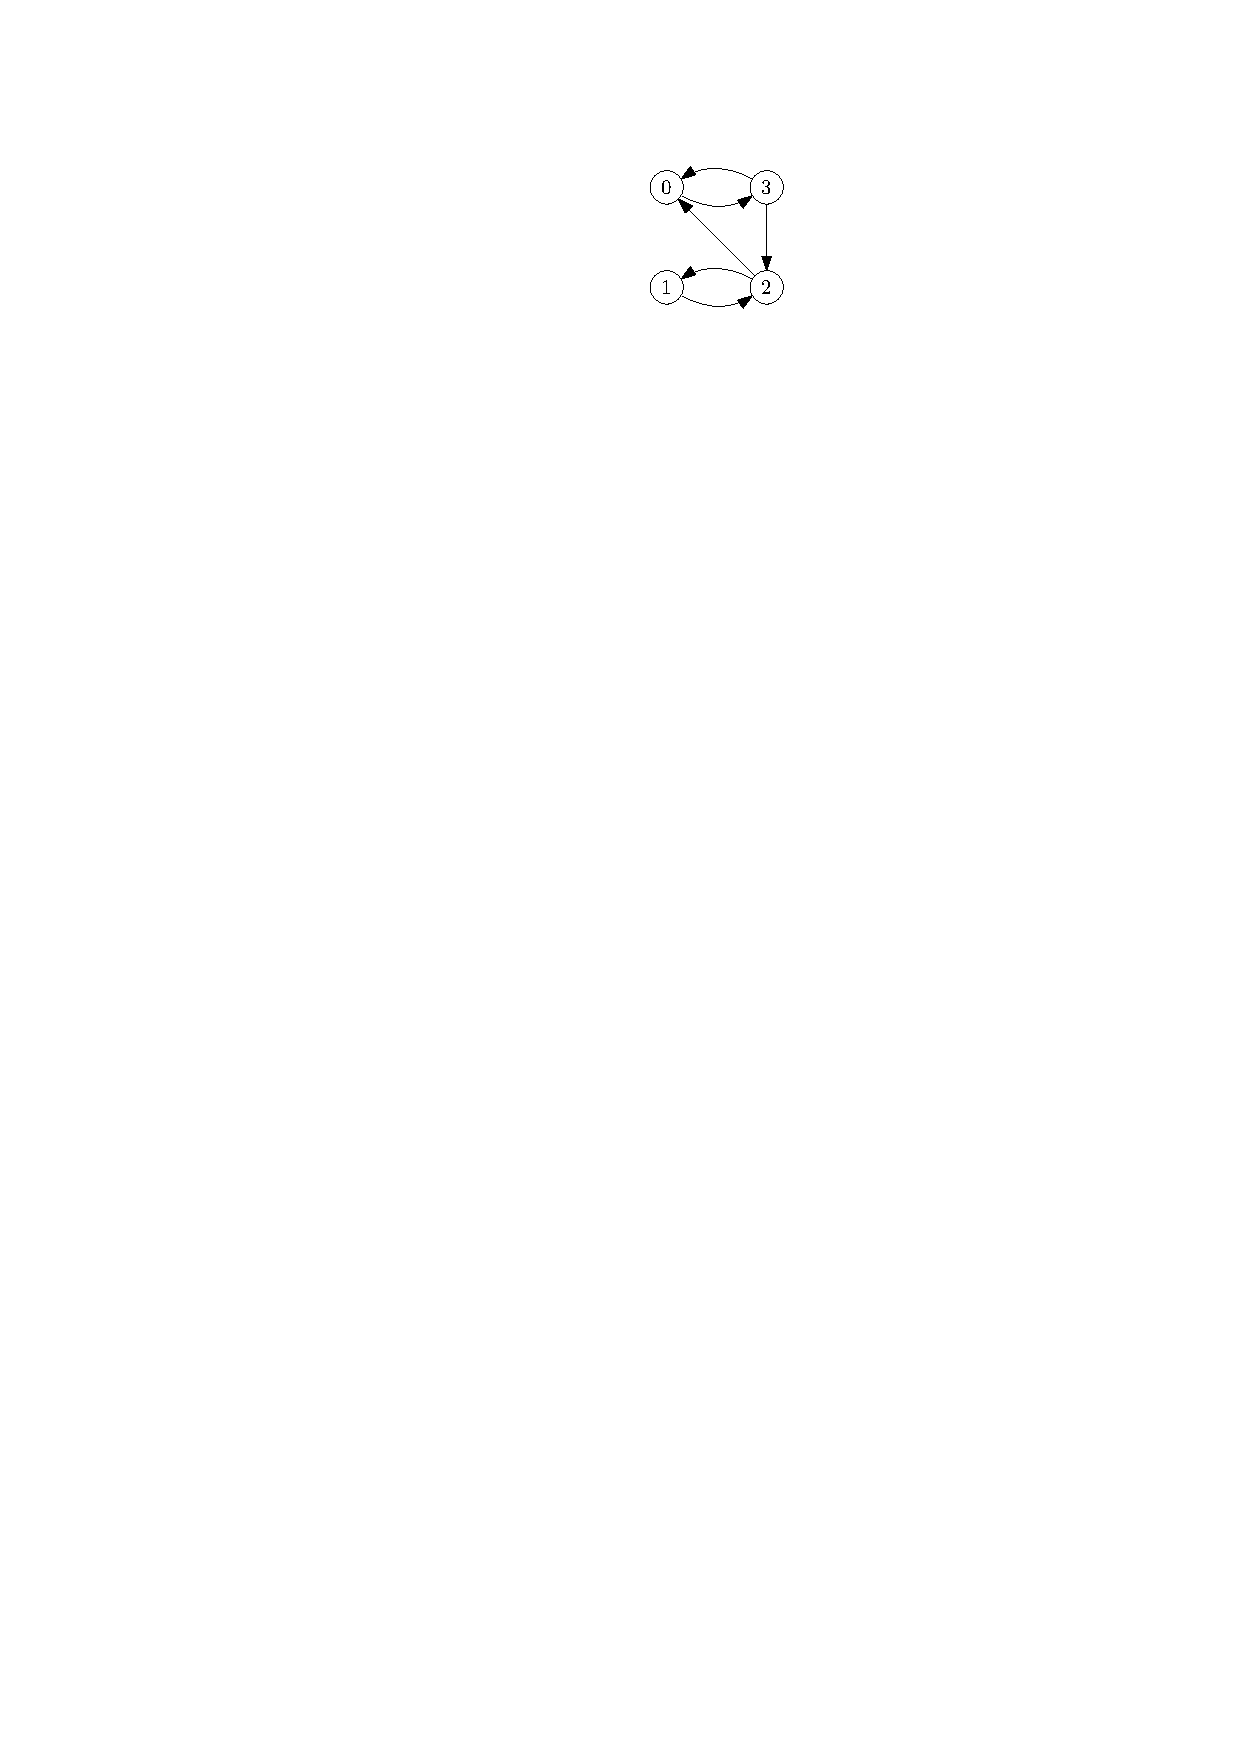
\includegraphics{graphEx5}
	\vspace{1cm}
	
Draw the digraph corresponding to the given adjacency lists.

	\vspace{1cm}
	$\lightgraybox{\begin{array}{c|ccc}
	0 & 1 & 2  \\
	1 & 3  \\
	2  \\
	3 & 0 & 1 & 2 \\
	\end{array}}$
\end{Boxample}

\section{Representing multiple graphs in a single file}
We can store several digraphs one after the other in a single file as follows: 
\begin{itemize}
  \item We have a single line giving the order at the beginning of each digraph.
  \item If the order is $n$ then the next $n$ lines give the adjacency matrix 
  or adjacency lists representation of the digraph. Node labels are omitted.
  \item The end of the file is marked with a line denoting a digraph of order $0$.
\end{itemize}

\begin{Boxample} 
The two digraphs on the left could be put in a single file:\\

\begin{minipage}[c]{0.5\textwidth}
\centering
	$\lightgraybox{\begin{array}{c|c}
	0 & 2  \\
	1 & 0  \\
	2 & 1 \\
	\end{array}}$
	
	\vspace{1cm}
	$\lightgraybox{\begin{array}{c|ccc}
	0 & 1 & 2  \\
	1 & 3  \\
	2  \\
	3 & 0 & 1 & 2 \\
	\end{array}}$
\end{minipage}
\begin{minipage}[c]{0.5\textwidth}
$$
\lightgraybox{
	\begin{array}{ccc}
	3 &   &   \\
	2 &   &   \\
	0 &   &   \\
	1 &   &   \\
	4 &   &   \\
	1 & 2 &   \\
	3 &   &   \\
	  &   &   \\
	0 & 1 &  2 \\
	0 &   &   \\
	\end{array}
}
$$
\end{minipage}
\end{Boxample}


\section{Using other structures to represent graphs}
Other specialized digraph representations may be used to take advantage of
special structure in a family of digraphs for improved storage or access time. 
For such specialized purposes they may be better than adjacency matrices or lists.

For example, trees can be stored more efficiently (c.f. \cref{sec:heapsort}).  
\begin{itemize}
\item A general rooted tree of $n$ nodes can be stored in array $\pred$ of size $n$. 
\item $\pred[i]$ is the parent of node $i$. 
\item The root has no parent, so assign it \texttt{null} or $-1$ if we number nodes from $0$
to $n-1$ in the usual way. 
\item This is a form of adjacency lists, using in-neighbours instead of out-neighbours.
\end{itemize}

\begin{Boxample}[4]
Draw the tree represented by the array $$\pred = [-1,0,0,1,2,2,2,3]\text{.}$$
\end{Boxample}

%\begin{Boxample}[5]
%Consider the digraph $G$ whose nodes are the integers from $1$ to $12$
%inclusive and such that $(i, j)$ is an arc if and only if $i$ is a
%proper divisor of $j$ (that is, $i$ divides $j$ and $i \neq j$).
%Write down the adjacency matrix representation of $G$ and of $G_r$.
%\end{Boxample}

\section{Implementation of digraph ADT} \label{sec:graphadtimpl}
An adjacency matrix is simply a matrix which is an array of arrays. 

Adjacency lists are a list of lists. 
There are several ways in which a list can be implemented, for
example by an array, or singly- or doubly-linked lists using pointers.  
These have different properties, for example, accessing the middle element is $\Theta(1)$ for an array but $\Theta(n)$ for a linked list. 
Searching for a value that may or may not be in the list requires sequential search
and takes $\Theta(n)$ time in the worst case. 
%
We do not consider other data structures (e.g. heaps) that can be used to represent lists. 

\section{Complexity of basic digraph operations}
The basic operations we consider are checking for the existence of an arc between two nodes, finding the outdegree of a node, 
finding the indegree of a node, adding an arc between two nodes, deleting an arc between two nodes, adding a node, and deleting a node. 

For the two data structures, consider the steps we need to carry out various basic operations and the cost of all steps. 

\begin{Boxample}
Compare the matrix and lists data structures for checking whether arc $(i,j)$ exists.\\
	\boldfont{Adjacency matrix representation}: 
	We need to check whether element $(i,j)$ is 1. 
	This requires accessing an array element twice, to first find the $i$th array then its $j$th element. 
	Each array access is in $\Theta(1)$ so overall it is in $\Theta(1)$.
	
	\boldfont{Adjacency lists representation}: We need to search for $j$ in list $i$. 
	The complexity then depends on the length of list $i$. 
	List $i$ is length $d$ where $d$ is the outdegree of node $i$ so searching for $j$ is in $\Theta(d)$. 
	But how large is $d$? 
	Even when the graph is sparse, it could still be the case that $d$ is $O(n)$,
	though typically in a sparse graph $d$ is $O(1)$.  
	In a dense graph $d$ is $O(n)$.
\end{Boxample}

\begin{Boxample}[3]
Compare the matrix/lists data structures for deleting a node.\\
	\boldfont{Adjacency matrix representation}: \vspace{3cm}
%	We must delete a row and column, and move up some elements so there are no gaps in the matrix. 
%	In the worst case, we need to move all remaining elements in the matrix 
%	and since there are now $(n-1)$s rows and columns, it takes time $\Theta(n^2)$.
	
	\boldfont{Adjacency lists representation}: 
%	We must remove a list and also all references to the deleted node in other lists. 
%	This requires scanning each list for the offending entry and deleting it. 
%	We thus need to visit $n$ lists and the combined length of all remaining lists which is (in the worst case) $m$, 
%	requiring $\Theta(n + m)$ work in total.
\end{Boxample}

\cref{tbl:basicOpsSteps} shows the steps required  
and \cref{tbl:basicOpsPerformance} the time required for basic graph operations 
when using adjacency matrix or lists representations.  
Performance for the adjacency list representation is based on using doubly linked lists.

\begin{table}[H]
\centering
\caption{Steps required to perform basic digraph operations by data structure.}
\label{tbl:basicOpsSteps}
\begin{tabular}{|l|l|l|}
\hline
\textbf{Operation} & \textbf{Adjacency matrix} & \textbf{Adjacency lists} \\
\hline
arc $(i, j)$ exists? & is entry $(i,j)$ 0 or 1  & find $j$ in  list $i$ \\
\hline
outdegree  of $i$ & scan row, count $1$'s & size of  list  $i$\\
\hline
indegree of $i$ & scan column,  count $1$'s & for $j\neq i$, find $i$ in list $j$ \\
\hline
add arc $(i, j)$ & change entry $(i ,j)$ & insert $j$ in list $i$ \\
\hline
delete arc $(i, j)$ & change entry $(i ,j)$ & delete $j$ from list $i$ \\
\hline
add node & create new row and column & add new list at end\\
\hline
delete node $i$ & delete row/column $i$  & delete list $i$ \\
& shuffle other entries & for $j\neq i$, delete  $i$ from list $j$ \\
\hline
\end{tabular}
\end{table}

\begin{table}[H]
\centering
\caption{Comparative worst-case performance of adjacency matrices and lists.}
\label{tbl:basicOpsPerformance}
\begin{tabular}{|l|c|c|}
\hline
\textbf{Operation} 	& \textbf{Adjacency matrix} & \textbf{Adjacency lists} \\
\hline
arc $(i, j)$ exists? & $\Theta(1)$  & $\Theta(d)$ \\
\hline
outdegree  of $i$ 	& $\Theta(n)$ & $\Theta(1)$ \\
\hline
indegree of $i$ 	& $\Theta(n)$ &  $\Theta(n+m)$ \\
\hline
add arc $(i, j)$ 	& $\Theta(1)$ & $\Theta(1)$  \\
\hline
delete arc $(i, j)$ & $\Theta(1)$  & $\Theta(d)$  \\
\hline
add node 			& $\Theta(n)$ & $\Theta(1)$  \\
\hline
delete node $i$ 	& $\Theta(n^2)$  & $\Theta(n+m)$  \\
\hline
\end{tabular}
\end{table}

Using lists, apparently similar problems like finding the outdegree ($\Theta(1)$) and indegree ($\Theta(n+m)$)
have very different time complexity. 
%\begin{itemize}
%  \item Finding the outdegree with lists merely requires accessing
%the correct list (constant time) plus finding the size of that list
%(constant time). 
%\item Finding the indegree with lists requires
%scanning all lists except one ($n-1$ of them), and looking at every arc in
%them, ($m$ arcs in the worst case), so taking time $\Theta(n+m)$. 
%\end{itemize}

Clearly finding all indegrees would be slow if we just used multiple calls to a method designed for getting the indegree of a single node. 

\begin{Boxample}[8]
Show that the sorted adjacency lists representation of the reverse digraph of $G$ can be found in time $\Theta(n+m)$ 
given the sorted adjacency lists of $G$. Also show how this can be used to find indegrees for all nodes of $G$ in time $\Theta(n+m)$.
\end{Boxample}

\section{Space requirements}
The adjacency matrix representation requires $\Theta(n^2)$ storage 
as we simply need a matrix of $n^2$ bits. 

At first guess we might say adjacency lists require $\Theta(n + m)$ storage, 
since we need $n$ lists and the combined length of all the lists is $m$.
But node numbers require more than one bit of storage each; the number $k$ uses about $\Theta(\log k)$ bits.
The average entry in a list is $\frac n 2$, so the total space requirement is more like $\Theta(n + m \log(n))$ 

\begin{Boxample}[5]
What is the storage requirement for a complete digraph on $n$ nodes, that is, a digraph where every possible arc
occurs?
\end{Boxample}

For small, sparse digraphs, lists use less space than a matrix, whereas for small
dense digraphs the space requirements are comparable. For large sparse
digraphs, a matrix can still be more efficient, but this happens rarely.

\begin{Boxample}[5]
Find a large sparse digraph where the matrix representation uses less space than the lists representation.
\end{Boxample}

The representation that is best will depend on the application and we cannot make general rules.  
We will mostly use adjacency lists, which are
clearly superior for many common tasks and generally better for sparse digraphs.


\part{Graph Traversals and Applications}
\label{ch:traversal}

\chapter{Graph traversal algorithms} %----------------------------------------
Traversals involve visiting each node of a digraph in a systematic way following only the arcs in the digraph. 
This is a very common task when dealing with digraphs and we will cover several applications in later lectures.

\section{The general graph traversal algorithm} \label{sec:trav}
All graph traversal algorithms have the same basic structure that relies on keeping track of which nodes have been visited 
and whether they may be adjacent to nodes that have not yet been visited. We use a system of three colours:
\begin{itemize} 
  \item \defnfont{White nodes} have not yet been visited;
  \item \defnfont{Grey nodes} (or \boldfont{frontier nodes}) have been visited but may have
  out-neighbours that are white;
  \item \defnfont{Black nodes} have been visited and all their out-neighbours have been visited too (so are not white). 
\end{itemize} 

\begin{Boxample}
Node states during a digraph traversal.
\begin{center}
  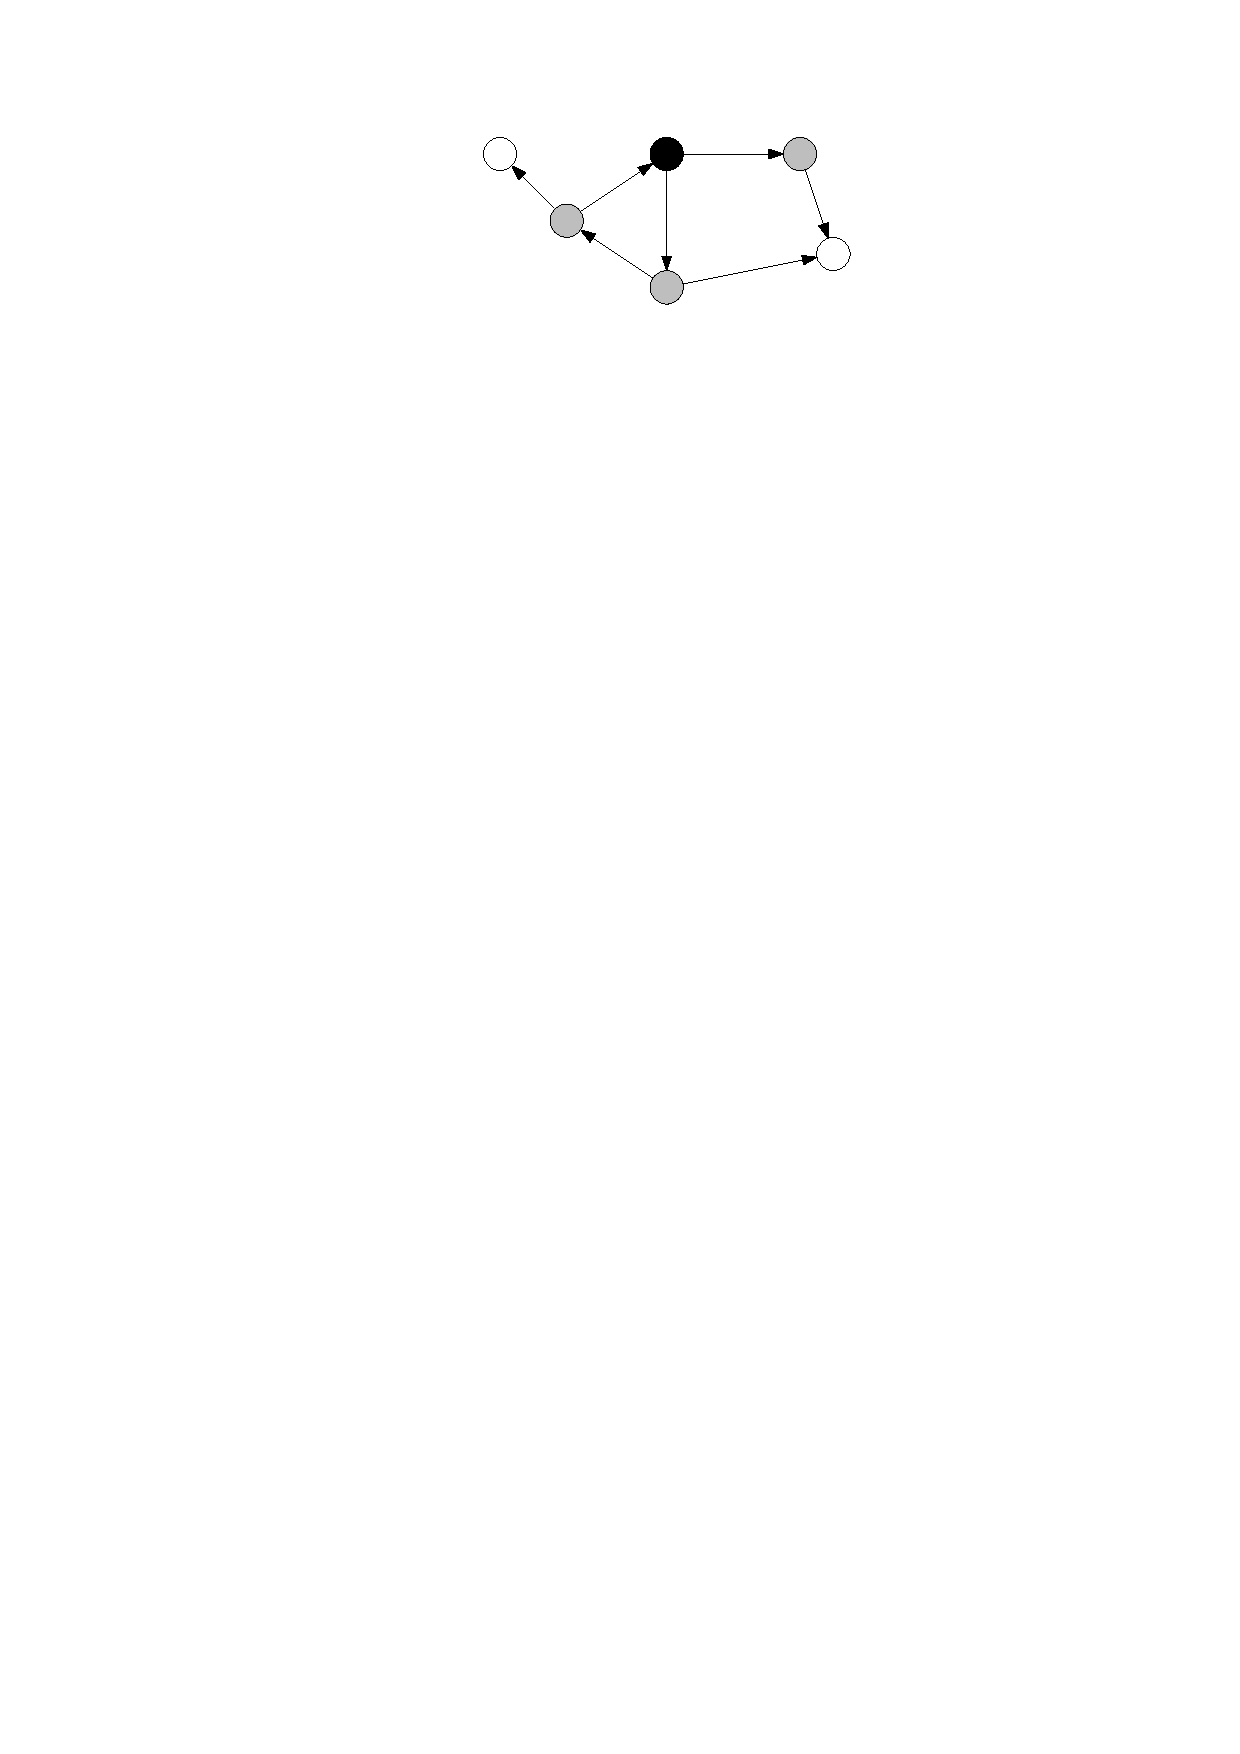
\includegraphics{graphTraversalNodeStateBW}
\end{center}
\end{Boxample}

The traversal algorithm which visits all nodes in a digraph is loosely described as follows: 
\begin{itemize}
  \item All nodes are white to begin with.
  \item A starting white node is chosen and turned grey.
  \item A grey node is chosen and its out-neighbours explored. 
  \item If any out-neighbour is white, it is visited and turned grey. 
  If no out-neighbours are white, the grey node is turned black. 
  \item The process of choosing grey nodes and exploring neighbours is continued 
  until all nodes reachable from the initial node are black.
  \item If any white nodes remain in the digraph, a new starting node is chosen 
  and the process continues until all nodes are black.
\end{itemize}

We keep track of the order in which nodes are visited by recording which arc was followed when a node first turned from white to grey. 
As we will see, this creates a sub-digraph of the original digraph which has a tree structure.

The traversal algorithm is formalised in the pseudocode of \cref{alg:traverse,alg:visit}.  
\cref{alg:traverse} (\algfont{traverse}) initialises the process and is tasked with finding white nodes to start from. 
Most of the work is done in \cref{alg:visit} (\algfont{visit}) which takes a starting node 
and explores the portion of the subgraph reachable from that node.

\begin{algorithm}[H]
  \caption{Basic graph traversal main routine: \algfont{traverse}}
  \label{alg:traverse}
\begin{algorithmic}[1]
\Function{traverse}{digraph $G$}
	\State array $\colour[0..n-1]$ \Comment{records node colour}
	\State array $\pred[0..n-1]$ \Comment{records path of traversal as a tree}
	\For{$u \in V(G)$} \Comment{make all nodes white}
		\State $\colour[u] \gets $ WHITE 
	\EndFor
	\For{$s \in V(G)$}  \Comment{find a white node}
		\If {$\colour[s] ==$ WHITE} 
			\State \texttt{visit}$(s)$ \Comment{start traversal from $s$}
		\EndIf
	\EndFor
	\Return $\pred$ 
\EndFunction
\end{algorithmic}
\end{algorithm}

\begin{algorithm}[H]
  \caption{Basic graph traversal subroutine: \algfont{visit}}
   \label{alg:visit}
\begin{algorithmic}[1]
\Function{visit}{node $s$ of digraph $G$}
	\State  $\colour[s] \gets$ GREY 
	\State $\pred[s] \gets$ \texttt{null} \Comment{make start node the root of the tree}
	\While{there is a GREY node} \Comment{continues until all nodes are black}
		\State choose a GREY node $u$ 
		\If{$u$ has a WHITE neighbour}
			\State choose a WHITE neighbour, $v$ 
			\State $\colour[v] \gets $ GREY \Comment{$v$ is visited for first time, so turns grey }
			\State $\pred[v] \gets u$ \Comment{make $u$ the parent of $v$ in the traversal tree}
		\Else
			\State $\colour[u] \gets $ BLACK \Comment{$u$ has no white neighbours so done with $u$ }
		\EndIf
	\EndWhile
\EndFunction
\end{algorithmic}
\end{algorithm}

A call to \texttt{visit} creates a subdigraph of $G$ that is a tree: 
the nodes are precisely the black nodes (all nodes reachable from the initial node), 
and the arcs are those arcs followed when we found a white neighbour of a grey node. 

Each white node chosen in \texttt{traverse} is the root of a tree in the call to \texttt{visit}. 
Eventually, we obtain a set of disjoint trees spanning the digraph (that is, it includes all the nodes of the digraph), 
which we call the \defnfont{search forest}. 
The search forest is returned by \texttt{traverse} in the array $\pred$.

\begin{Boxample}
Traversal of a digraph.
\begin{center}
  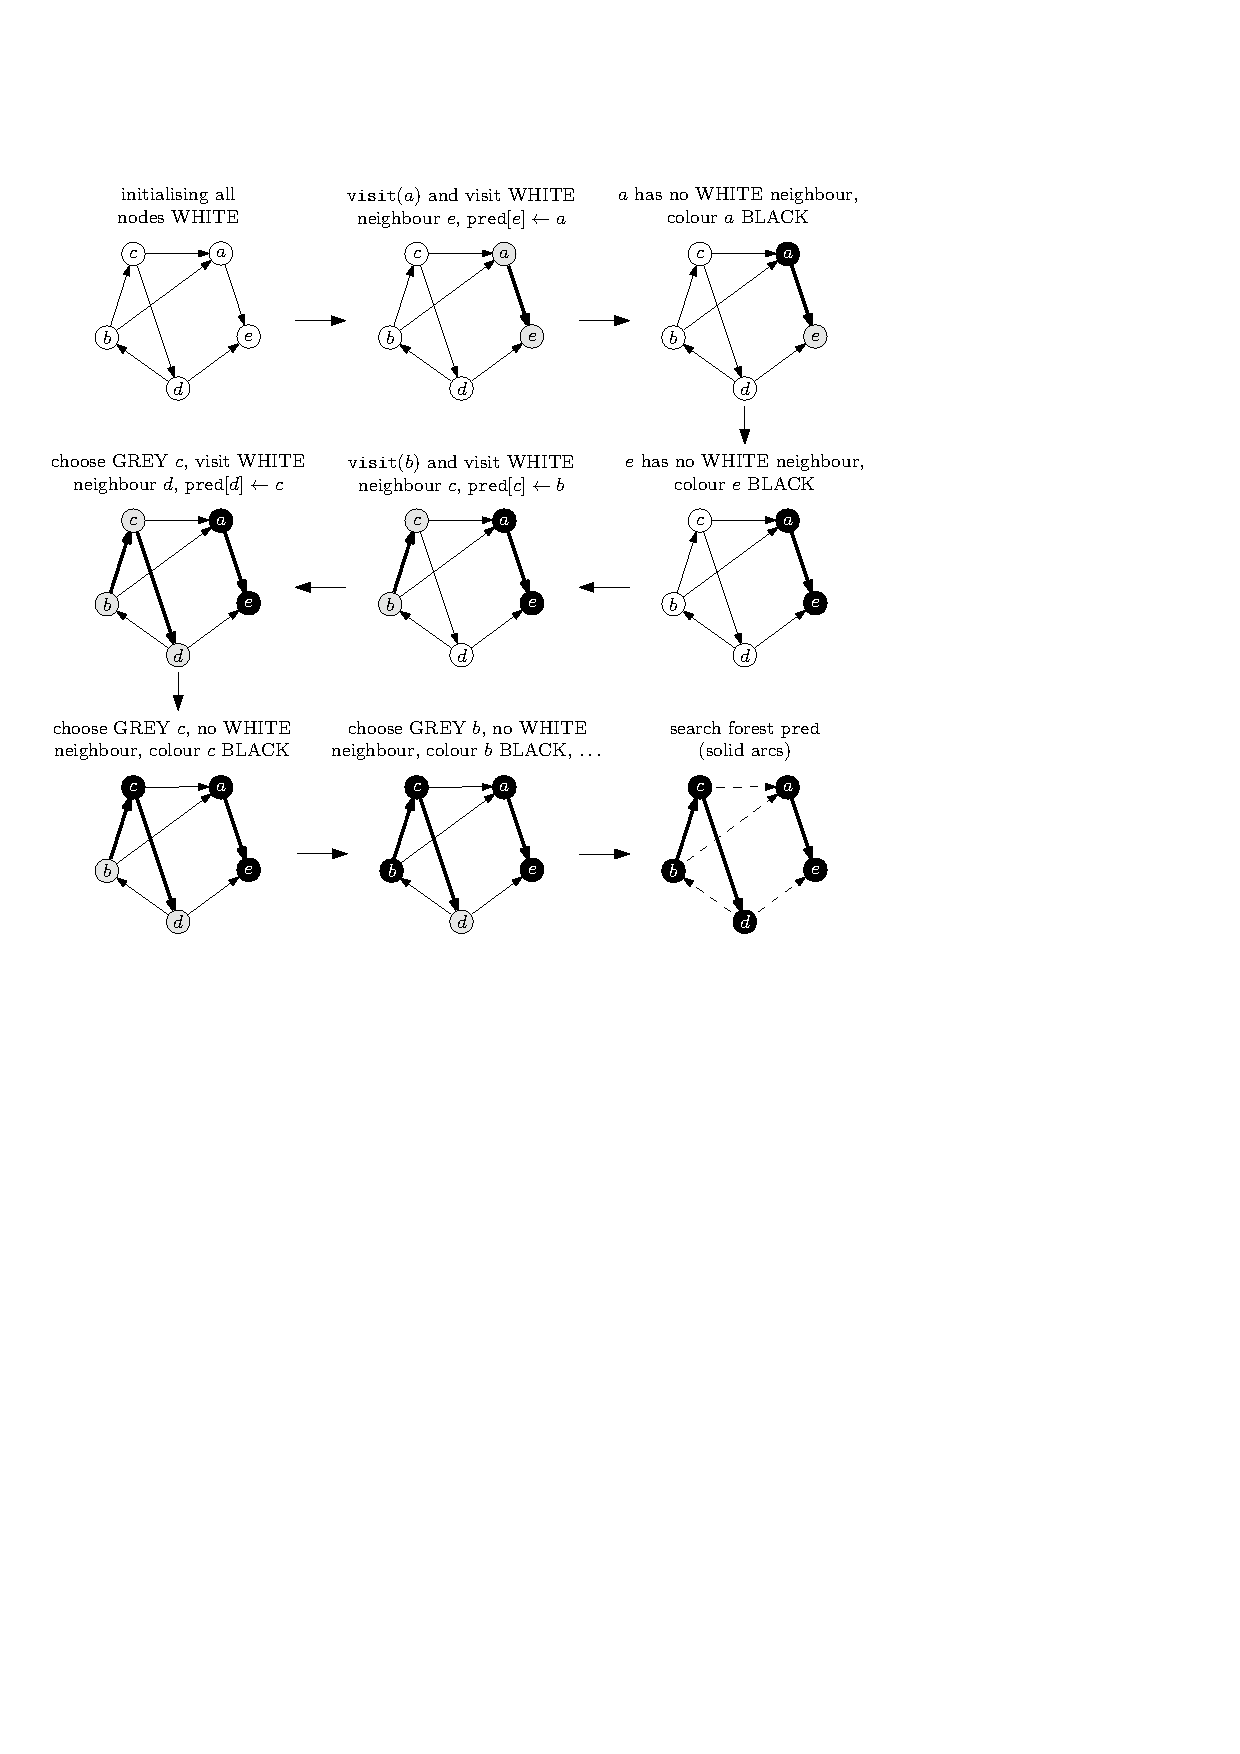
\includegraphics[width=1.0\linewidth]{traversalAlgoEx}
\end{center}
\end{Boxample}

\section{Classifying arcs after a traversal}
It helps in analysing the traversal algorithm to classify the arcs of $G$ based on their relationships in the search forest.  

\begin{Definition} \label{defn:arc-types}
Suppose we have performed a traversal of a digraph $G$, resulting in a search forest $F$. 
Let $(u, v)\in E(G)$ be an arc. Then $(u, v)$ is a
\begin{itemize} 
  \item \defnfont{tree arc} if it belongs to one of the trees of $F$;
  \item or, if it is not a tree arc, it is a
  \begin{itemize}
	\item \defnfont{forward arc} if $u$ is an ancestor of $v$ in $F$;
	\item \defnfont{back arc} if $u$ is a descendant of $v$ in $F$; 
	\item \defnfont{cross arc} if neither $u$ nor $v$ is an ancestor of the other in $F$.
  \end{itemize}
\end{itemize}
\end{Definition} 

A cross arc may join two nodes in the same tree or point from one tree to another in the search forest. 
Tree, forward and back arcs require that $u$ and $v$ be in the same tree.

\begin{Boxample}
Classify the arcs according to the definitions above. 

\begin{center}
  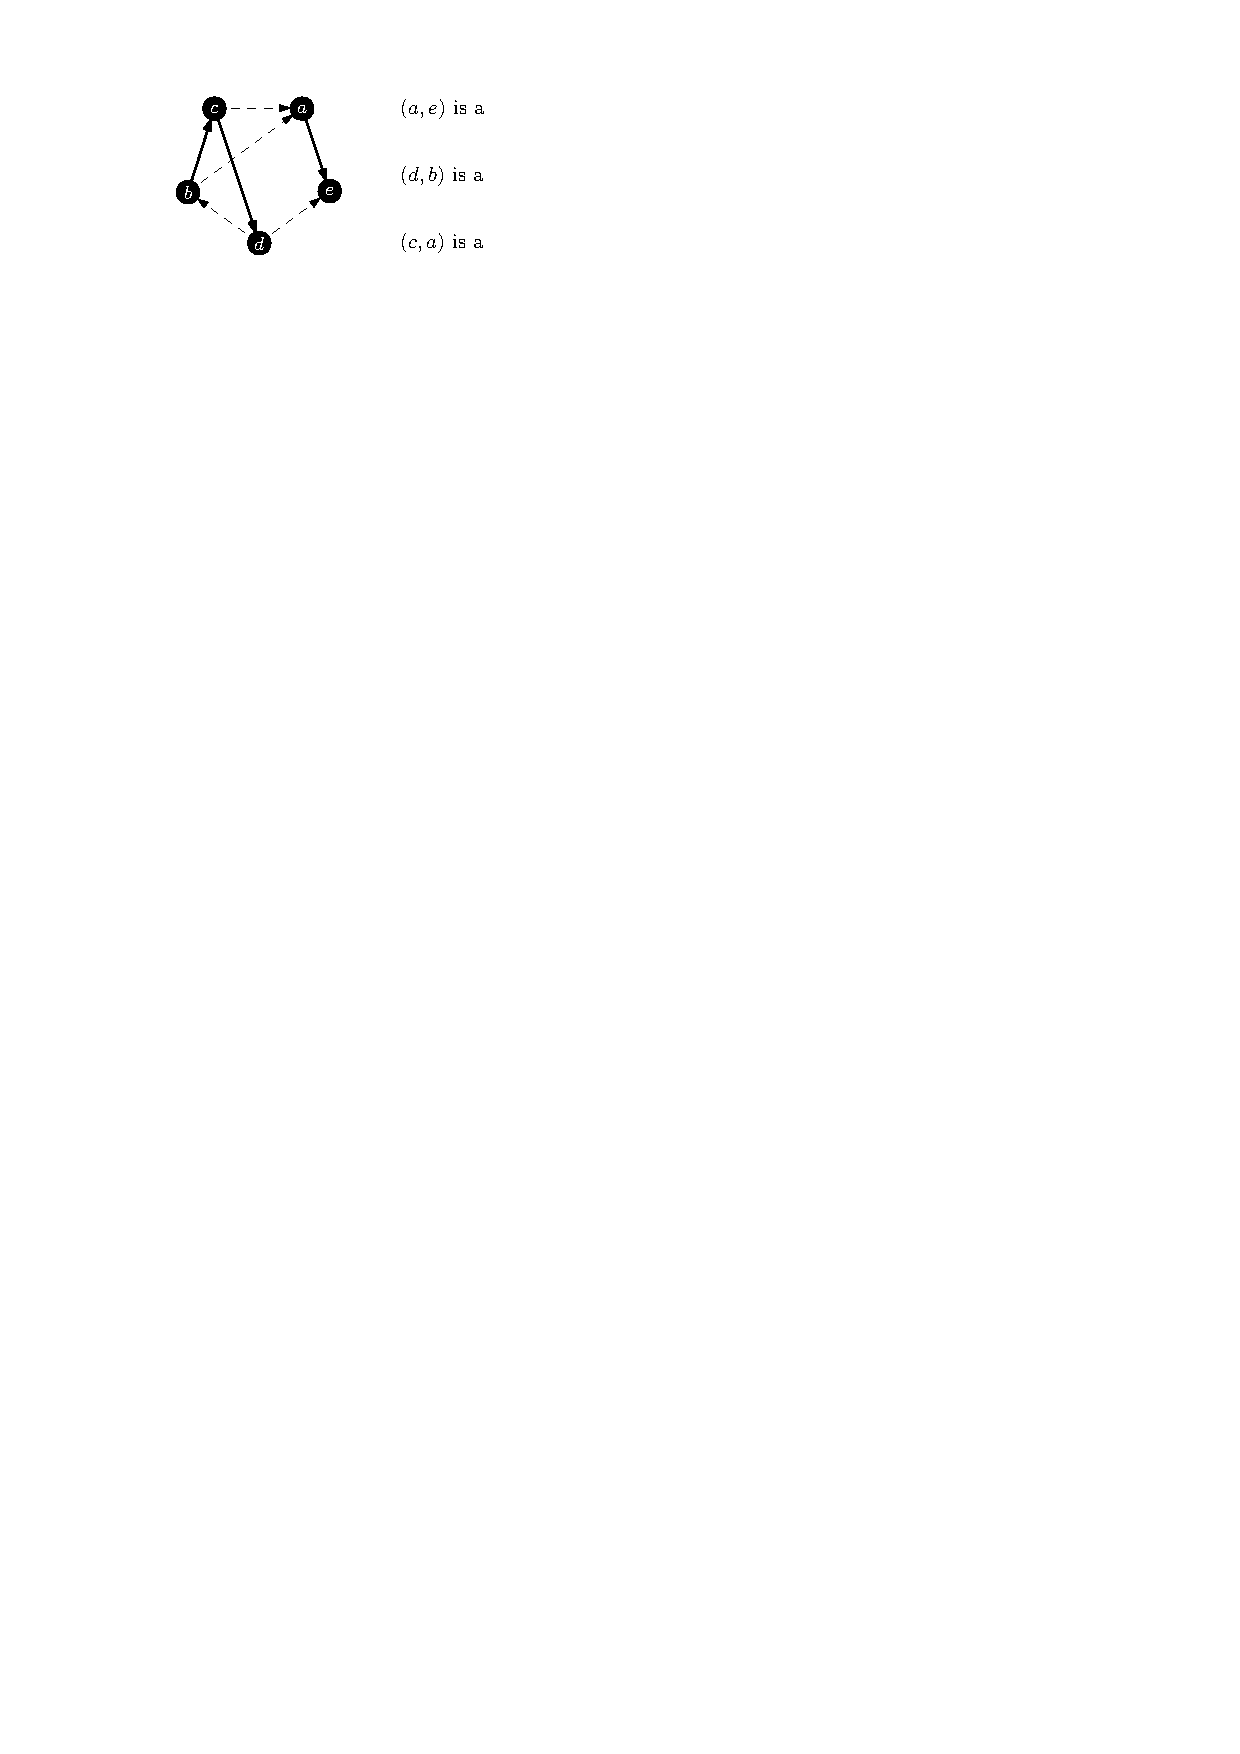
\includegraphics{traversalAlgoResultEx} 
\end{center}
\end{Boxample}

The following theorem collects all the basic facts we need for proofs
in later sections. The proofs are simple and can be done as exercises. 

\begin{Theorem} \label{thm:trav}
Suppose that we have carried out \texttt{traverse} on $G$, 
resulting in a search forest $F$. Let $v, w \in V(G)$.
\begin{itemize}
  \item Let $T_1$ and $T_2$ be different trees in $F$ and suppose that $T_1$ was explored before $T_2$. 
  Then there are no arcs from $T_1$ to $T_2$. 
  \item Suppose that $G$ is a graph. Then there can be no edges joining different trees of $F$.
  \item Suppose that $v$ is visited before $w$ and $w$ is reachable from $v$ in $G$. 
  Then $v$ and $w$ belong to the same tree of $F$.
  \item Suppose that $v$ and $w$ belong to the same tree $T$ in $F$. 
  Then any path from $v$ to $w$ in $G$ must have all nodes in $T$.
\end{itemize}
\end{Theorem}
%\begin{proof}
%If the first part were not true, then since $w$ is reachable from $v$,
%and $w$ has not been visited before $T_1$ is started, $w$ must be reached
%in the generation of $T_1$, contradicting $w\in T_2$. The second part
%follows immediately for symmetric digraphs and hence for graphs. Now
%suppose that $v$ is seen before $w$. Let $r$ be the root of the tree $T$
%containing $v$. Then $w$ is reachable from $r$ and so since it has not
%already been visited when $r$ is chosen, it belongs to $T$. Finally, if
%$v$ and $w$ are in the same tree, then any path from $v$ to $w$ in $G$
%going outside the tree must re-enter it via some arc; either the leaving
%or the entering arc will contradict the first part.
%\end{proof}

\begin{Boxample}[5]
Assuming the first statement of \cref{thm:trav}, prove the third statement.
\end{Boxample}

\section{Running time for the general traversal algorithm}
The generality of our traversal algorithm makes it exact running time impossible to determine.  
It depends on how one chooses the next grey node $u$ and its white neighbour $v$.  
Some schemes for choosing $u$ and $v$ can be complex and depend on $n$. 
The schemes we consider here are simple and constant time.

% It also apparently depends on how long it takes to determine 
% whether there exist any grey nodes or whether $u$ has any white neighbours. 
% However, any sensible rule for checking existence of either type of node 
% should simply return false if there is no such node, 
% and take no more time in this case than if it does find one. 
% Thus we do not need to take account of the checking in our analysis.

\begin{itemize}
  \item The initialization of the array $\colour$ takes time $\Theta(n)$ so \texttt{traverse} 
  is in $\Theta(n + t)$, where $t$ is the total time taken by all the calls to \texttt{visit}.
  \item We execute the while-loop of \texttt{visit} in total $\Theta(n)$ times 
  since every node must eventually move from white through grey to black. 
  \item The time taken in choosing grey nodes is $\Omega(n)$. 
  \item The time taken to find a white neighbour involves examining each neighbour of $u$ 
  and checking whether it is white, then applying a selection rule. 
  \item The total time in choosing white neighbours is in $\Omega(m)$ if adjacency lists are used 
  and is in $\Omega(n^2)$ if an adjacency matrix is used.
  \item So the running time of \texttt{traverse} is $\Omega(n + (n+m)) = \Omega(n + m)$
  if adjacency lists are used, and $\Omega(n + n^2) = \Omega(n^2)$ if the adjacency matrix format is used.
\end{itemize}

So for simple selection rules and assuming a sparse input digraph, the adjacency list format seems
preferable. But if more complex selection rules are used, for example, choosing a single grey node is 
of order $n$ while choosing a single white node is still constant time, then the running time is 
asymptotically $\Omega(n^2)$ regardless of the data structure, so using
the adjacency matrix is not clearly ruled out.


\chapter{Depth first search (DFS)} %------------------------------------------------
Traversal algorithms differ in the rules for choosing the next grey and next white node, 
with different rules leading to very different results.

\begin{Definition}
In \defnfont{depth-first search} (DFS) the new grey node chosen is the one
that has been grey for the \boldfont{shortest} time.
\end{Definition}

DFS takes us away from the root node as quickly as possible. 
If the first visited neighbour of the root has a neighbour, we immediately visit that neighbour. 
Then, if that has a neighbour, we visit that and so on, thus ``deeply'' searching as far away from the root as possible. 
We backtrack as little as possible before continuing away from the root again. The root is the last node to turn black.

There still remains the choice of which white neighbour of the chosen grey node to visit. 
It does not matter what choice is made but our \boldfont{convention is to choose the one with
lowest index} (recall that nodes have indices $0, \dots, n - 1$). 

These choices can be made in constant time so that the running time is  $\Omega(n + m)$ (assuming adjacency lists) 
and DFS is linear in the size $+$ order of a digraph. 

\begin{Boxample}[2]
A digraph and its DFS search tree, rooted at node $0$. The dashed arcs indicate the original arcs that are not part of the DFS search tree.
\begin{center}
  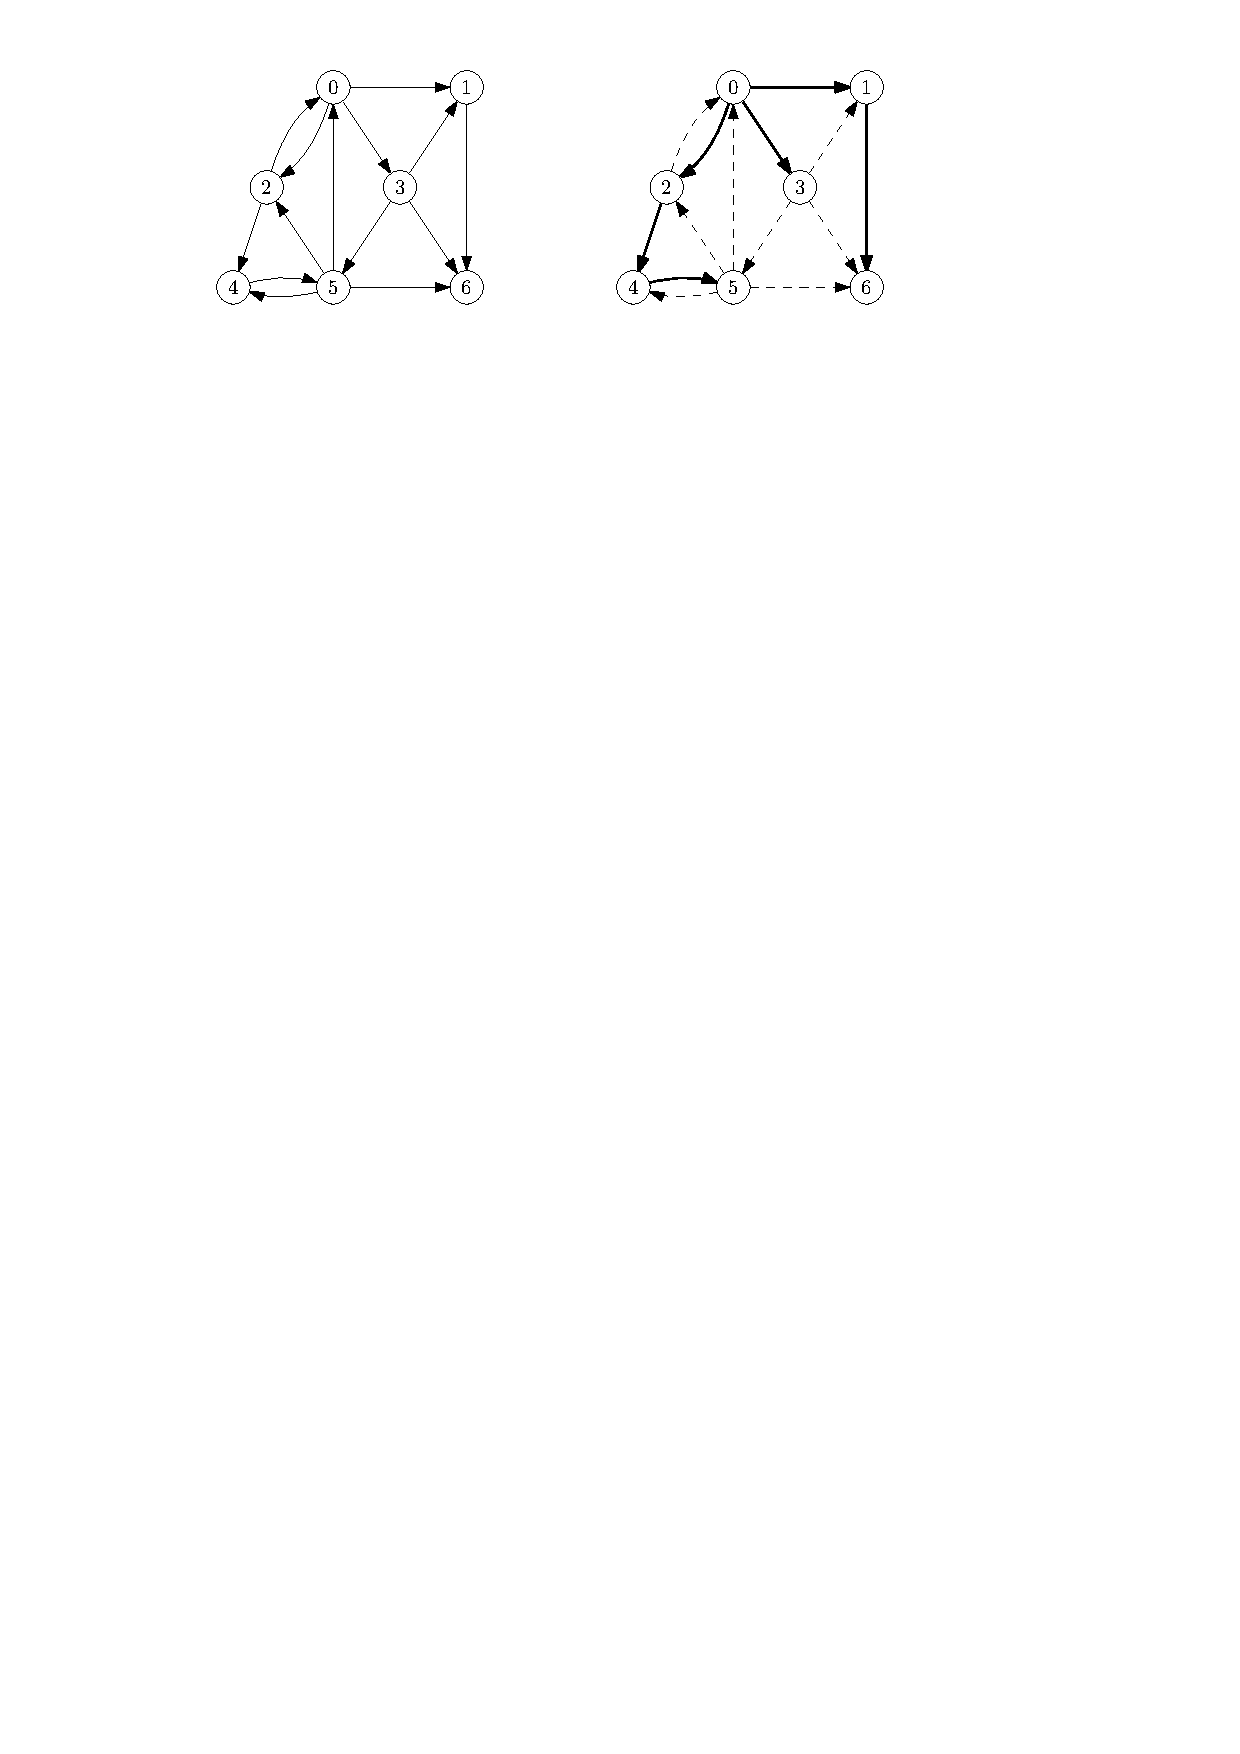
\includegraphics{DFSalgoDigraph}
\end{center}
Find a tree arc, cross arc, forward arc and back arc (or say if that type of arc does not exist for that traversal).
\end{Boxample}

\begin{Boxample}[2]
Use the nodes on the right to draw the search tree you obtain by running DFS on the graph on the left, starting at vertex $0$. 
Use dashed edges to indicate edges that are not arcs in the search tree.
\begin{center}
  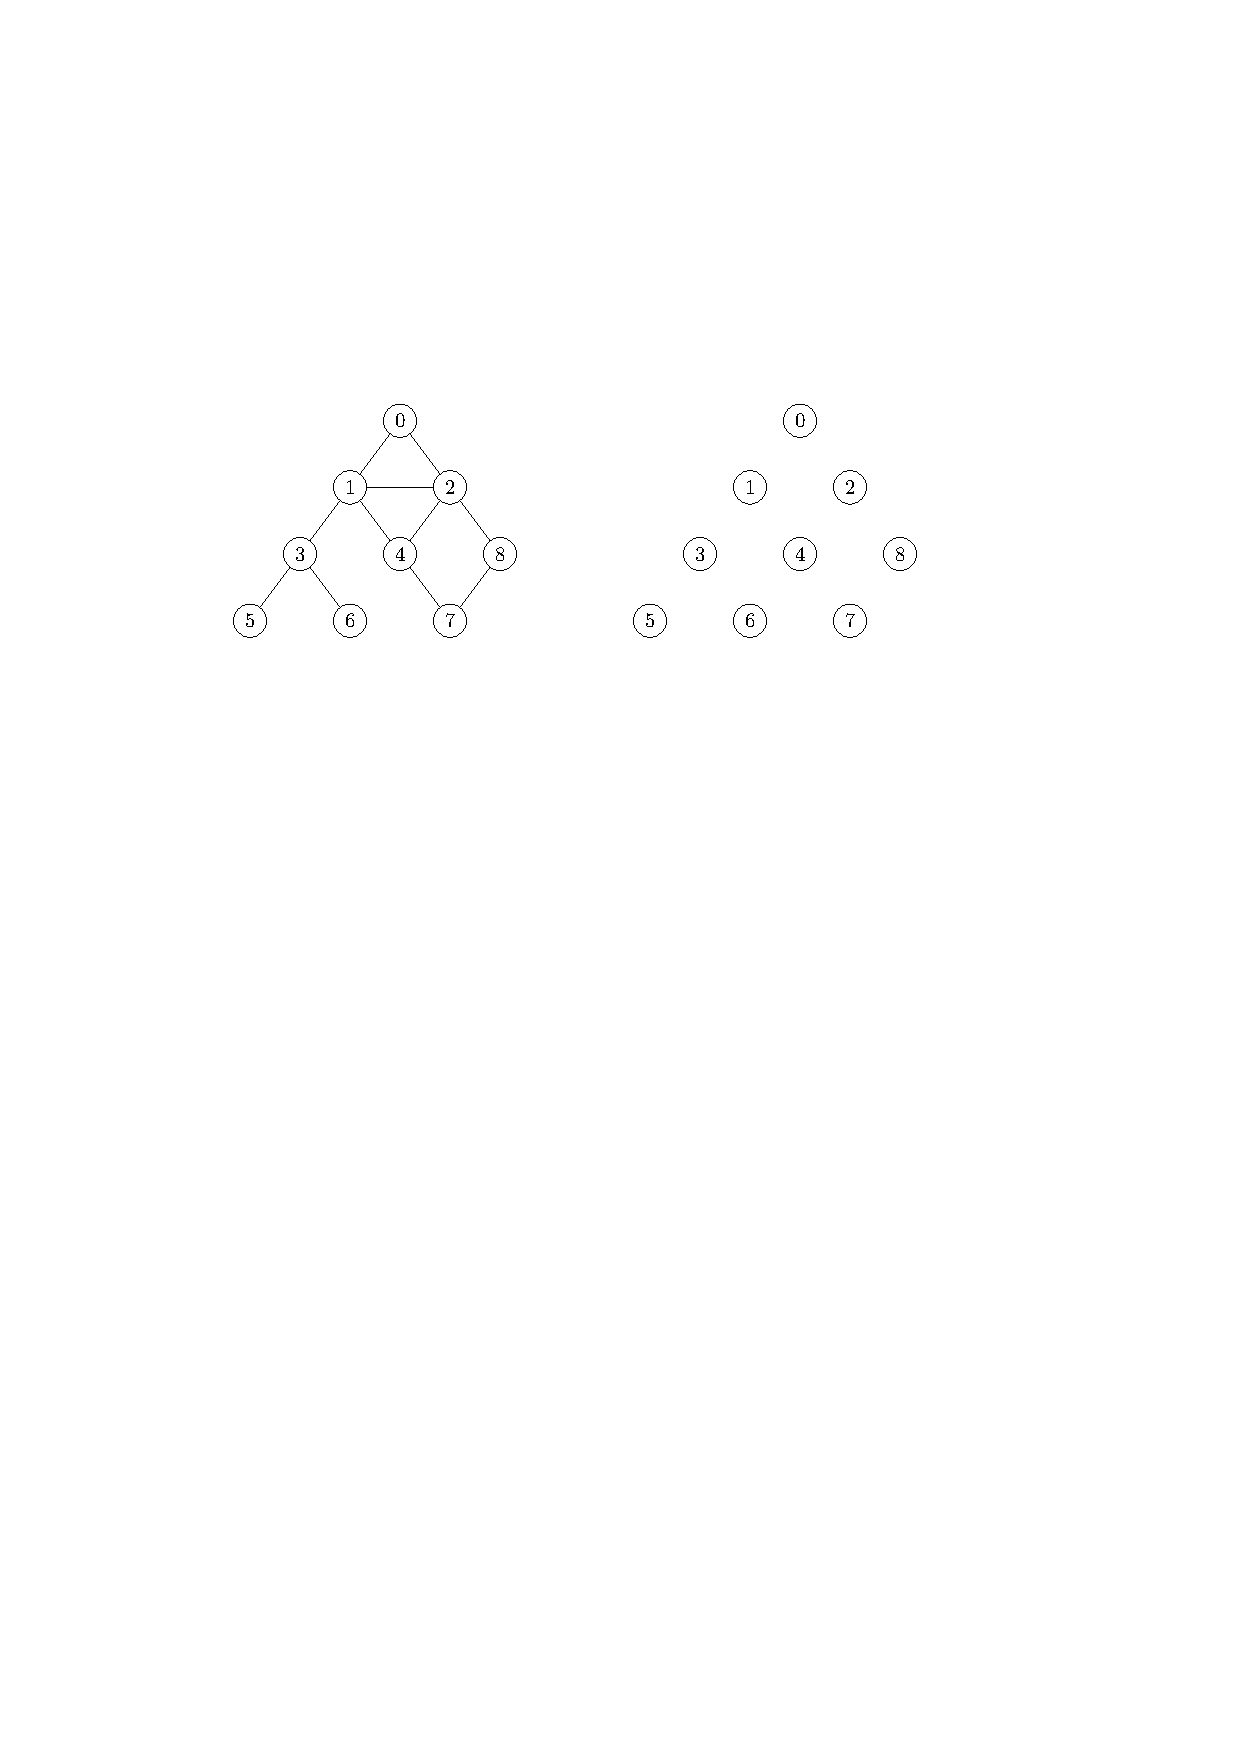
\includegraphics{TraverseGraphEx} 
\end{center}
Find a tree arc, cross arc, forward arc and back arc (or say if that type of arc does not exist for that traversal).
\end{Boxample}

For a general digraph, and unlike the examples given here, all nodes may not be reachable from the starting node. 
In this case, we get a search forest where the number of trees in the forest is the number of calls made to \texttt{DFSvisit}.

\section{Pseudocode for depth-first search} \label{ss: DFS}
The ``last in, first out" order of choosing grey nodes in DFS is mimicked by a \boldfont{stack} data structure. 
We thus store grey nodes in a stack as they are discovered. 

The pseudocode for \algfont{DFS} and \algfont{DFSvisit} is in \cref{alg:DFScode,alg:DFSvisitcode}. 
\begin{itemize}
  \item We loop through the nodes adjacent to the chosen grey node $u$, 
  and as soon as we find a white one, we add it to the stack.
  \item We also introduce a variable $\timeVar$ and keep track of the time a node changes colour
  \item The array $\seen$ records the time a node turns grey
  \item The array  $\done$ records the time a node turns black
\end{itemize}

\begin{algorithm}[H]
  \caption{Depth-first search algorithm.}
    \label{alg:DFScode}
\begin{algorithmic}[1]
\Function{DFS}{digraph $G$}
	\State stack $S$ 
	\State array $\colour[0..n-1]$, $\pred[0..n-1]$, $\seen[0..n-1]$, $\done[0..n-1]$
	\For{$u \in V(G)$}  
		\State $\colour[u] \gets $ WHITE; $\pred[u] \gets $ \texttt{null} \Comment{initialise arrays}
	\EndFor
	\State $\timeVar \gets 0$ \Comment{time will increment at every node colour change}
	\For{$s \in V(G)$} 
		\If{$\colour[s] = $ WHITE}  \Comment{find a WHITE node}
			\State \texttt{DFSvisit}$(s)$ \Comment{start traversal from $s$}
		\EndIf
	\EndFor
	\State \Return{$\pred, \seen, \done$}
\EndFunction
\end{algorithmic}
\end{algorithm}

\begin{algorithm}[H]
  \caption{Depth-first visit algorithm.}
    \label{alg:DFSvisitcode}
\begin{algorithmic}[1]
\Function{DFSvisit}{node $s$}
	\State $\colour[s] \gets $ GREY 
	\State $\seen[s] \gets \timeVar$; $\timeVar \gets \timeVar + 1$
	\State $S$.\texttt{insert}$(s)$ \Comment{put $s$ in stack}
	\While{\textbf{not} $S$.\texttt{isEmpty}$()$}
		\State $u \gets S$.\texttt{peek}$()$  \Comment{get node at front of stack}
		\If{there is a neighbour $v$ with $\colour[v] = $ WHITE}
			\State $\colour[v] \gets $ GREY; $\pred[v] \gets u$  \Comment{visit neighbour, update tree}
			\State $\seen[v] \gets \timeVar$; $\timeVar \gets \timeVar + 1$  \Comment{record and increment time}
			\State $S$.\texttt{insert}$(v)$  \Comment{put neighbour in stack}
		\Else
			\State $S$.\texttt{delete}$()$  \Comment{delete node from stack}
			\State $\colour[u] \gets $ BLACK  \Comment{colour it done}
			\State $\done[u] \gets \timeVar$; $\timeVar \gets \timeVar + 1$  \Comment{record and increment time}
		\EndIf
	\EndWhile
\EndFunction
\end{algorithmic}
\end{algorithm}

Given the relationship between stacks and recursion, we can replace the \texttt{DFSvisit} procedure by
a recursive version \algfont{recursiveDFSvisit}: 

\begin{algorithm}[H]
  \caption{Recursive DFS visit algorithm.}
    \label{alg:DFSreccode}
\begin{algorithmic}[1]
\Function{recursiveDFSvisit}{node $s$}
	\State $\colour[s] \gets $ GREY \
	\State $\seen[s] \gets \timeVar$; $\timeVar \gets \timeVar + 1$
	\For{each $v$ adjacent to $s$}
		\If{$\colour[v] = $ WHITE} \Comment{each unvisited neighbour}
			\State $\pred[v] \gets s$ \Comment{update tree}
			\State \texttt{recursiveDFSvisit}$(v)$ \Comment{now visit neighbour}
		\EndIf
	\EndFor
	\State $\colour[s] \gets $ BLACK \Comment{visted all white neighbours so done}
	\State $\done[s] \gets \timeVar $; $\timeVar \gets \timeVar + 1$
\EndFunction
\end{algorithmic}
\end{algorithm}

\begin{Boxample} \label{ex:DFSrecursive}
DFS with \texttt{recursiveDFSvisit}. 
\begin{center}
  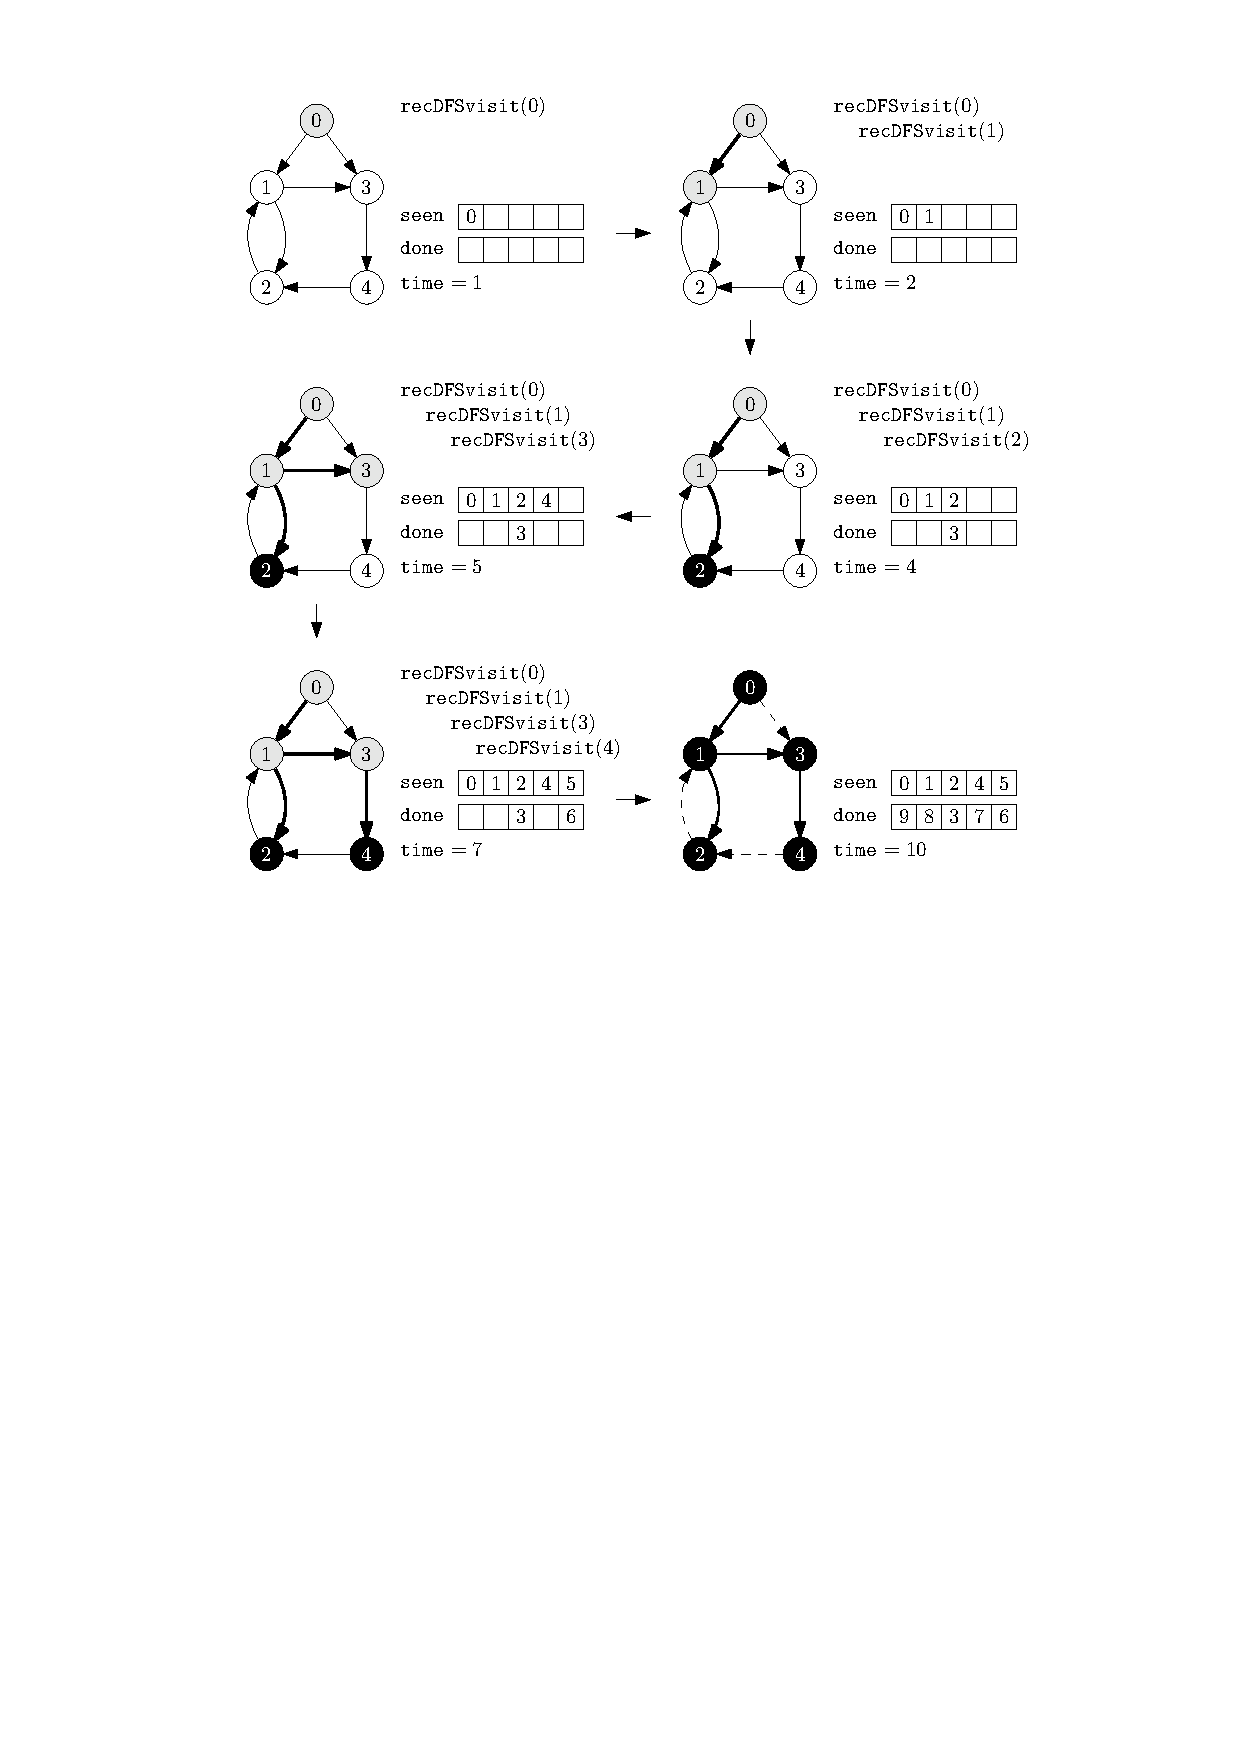
\includegraphics[width=1.0\linewidth]{DFSalgoRecursive2}
\end{center}
\end{Boxample}

\begin{Boxample}
Execute DFS with \texttt{recursiveDFSvisit} and following \cref{ex:DFSrecursive} fill out the values for $\seen$ and $\done$, give the current \texttt{time}, 
and highlight the DFS search tree after each step. 

\begin{center}
  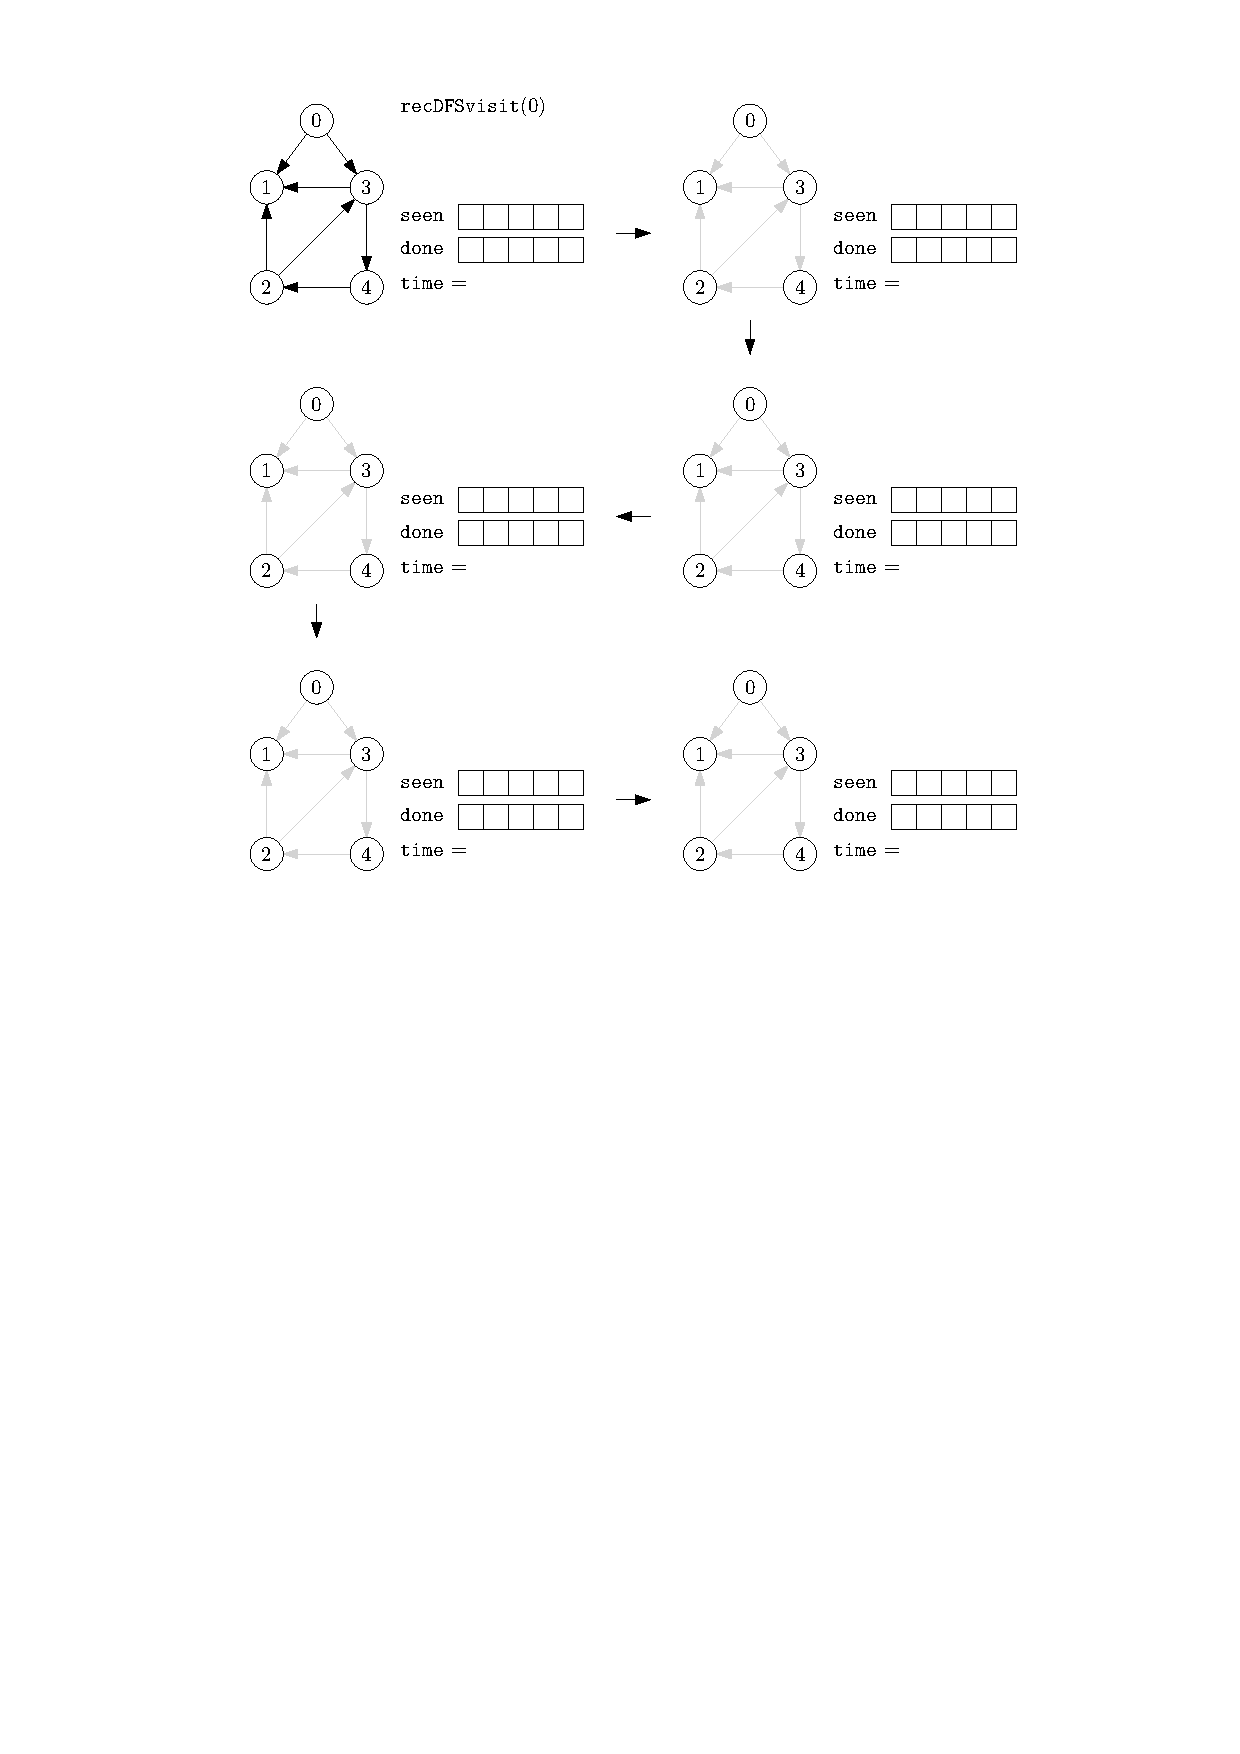
\includegraphics[width=1.0\linewidth]{DFSalgoRecursiveEx}
\end{center}
\end{Boxample}

\section{DFS useful results and facts}
\begin{Theorem}
\label{thm:DFS-seen-done}
Suppose that we have performed DFS on a digraph $G$, resulting in a 
search forest $F$. Let $v, w \in V(G)$ and suppose that $\seen[v] < \seen[w]$. 

\begin{itemize}
\item
If $v$ is an ancestor of $w$ in $F$, then 
$$\seen[v] < \seen[w] < \done[w] < \done[v].$$
\item
If $v$ is not an ancestor of $w$ in $F$, then
$$\seen[v] < \done[v]  < \seen[w] < \done[w].$$
\end{itemize}
\end{Theorem}
%\begin{proof} The first part is clear from the recursive formulation
%of DFS. Now suppose that $v$ is not an ancestor of $w$. Note that $w$
%is obviously also not an ancestor of $v$. 
%%Let $x$ be the root of the tree of $F$ containing $v$. 
%Thus $v$ lives in a subtree that is completely explored before the 
%subtree of $w$ is visited by \texttt{recursiveDFSvisit}.
%\end{proof}

Note that this result rules out  the timestamps $\seen[v] < \seen[w] < \done[v] < \done[w]$.

All four types of arcs in our search forest classification can
arise with DFS. The different types of arcs can be easily
distinguished while the algorithm is running or by looking at the timestamps 
$\seen$ and $\done$.

\begin{Boxample}[5]
Explain how to determine, at the time when an arc is first explored by
\texttt{DFS}, whether it is a tree-, back-, forward- or cross-arc.
\end{Boxample}

\begin{Boxample}[5] \label{ex:DFS-arc-class}
Suppose that we have performed \texttt{DFS} on a digraph $G$.
 Let $(v, w)\in E$. The following statements are true. Prove the first statement.
\begin{itemize}
  \item $(v, w)$ is a tree or forward arc if and only if  
	$$\seen[v] < \seen[w] < \done[w] < \done[v]\text{;}$$
  \item $(v, w)$ is a back arc if and only if
	$$\seen[w] <  \seen[v] < \done[v] < \done[w]\text{,}$$ 
  \item $(v, w)$ is a cross arc if and only if 
	$$\seen[w] < \done[w]  < \seen[v] < \done[v]\text{.}$$
\end{itemize}
\end{Boxample}

%\begin{Boxample}[3] \label{ex:DFS-graph-no-cross}
%Suppose that DFS is run on a graph $G$. Prove that cross edges do not occur.
%\end{Boxample}


\chapter{Breadth First Search (BFS) and Priority\\ First Search (PFS)} %------------------
\begin{Definition}
In \defnfont{breadth-first search} (BFS) the new grey node chosen is the one
that has been grey for the \boldfont{longest} time
\end{Definition}
 
BFS takes us away from the root node as slowly as possible. 
First we visit the root, then all its neighbours, then all neighbours of its neighbours and so on. 
The root is the first node to turn black.

As with DFS, the running time of BFS is in $\Theta(n+m)$ when implemented using adjacency lists.

\begin{Boxample}[4]
A digraph and its BFS search tree, rooted at node $0$. 
The dashed arcs indicate the original arcs that are not part of the BFS search tree.
\begin{center}
  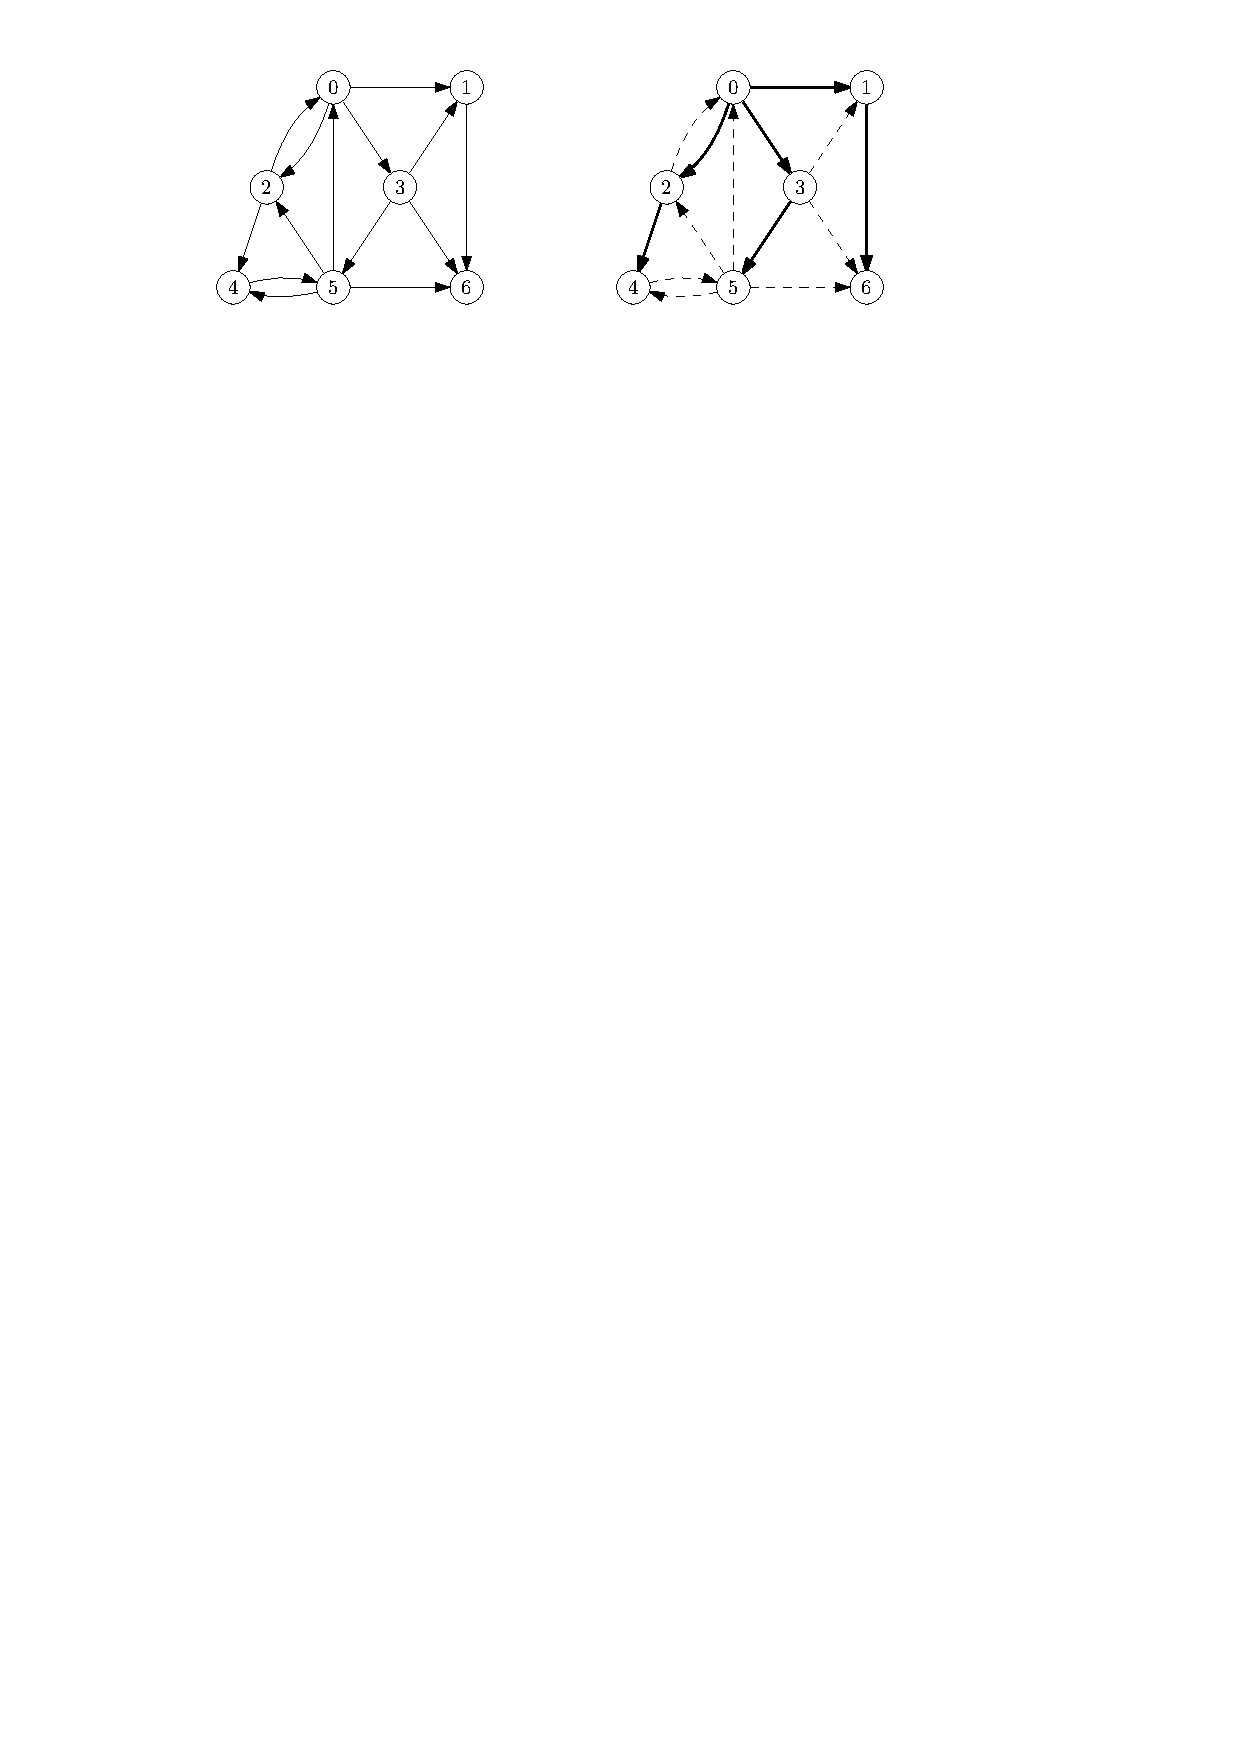
\includegraphics{BFSalgoDigraph} 
\end{center}
Find a tree arc, cross arc, forward arc and back arc (or say if that type of arc does not exist for that traversal).
\end{Boxample}

\begin{Boxample}[4]
Use the nodes on the right to draw the search tree you obtain by running BFS on the graph on the left, starting at vertex $0$. 
Use dashed edges to indicate edges that are not arcs in the search tree.
\begin{center}
  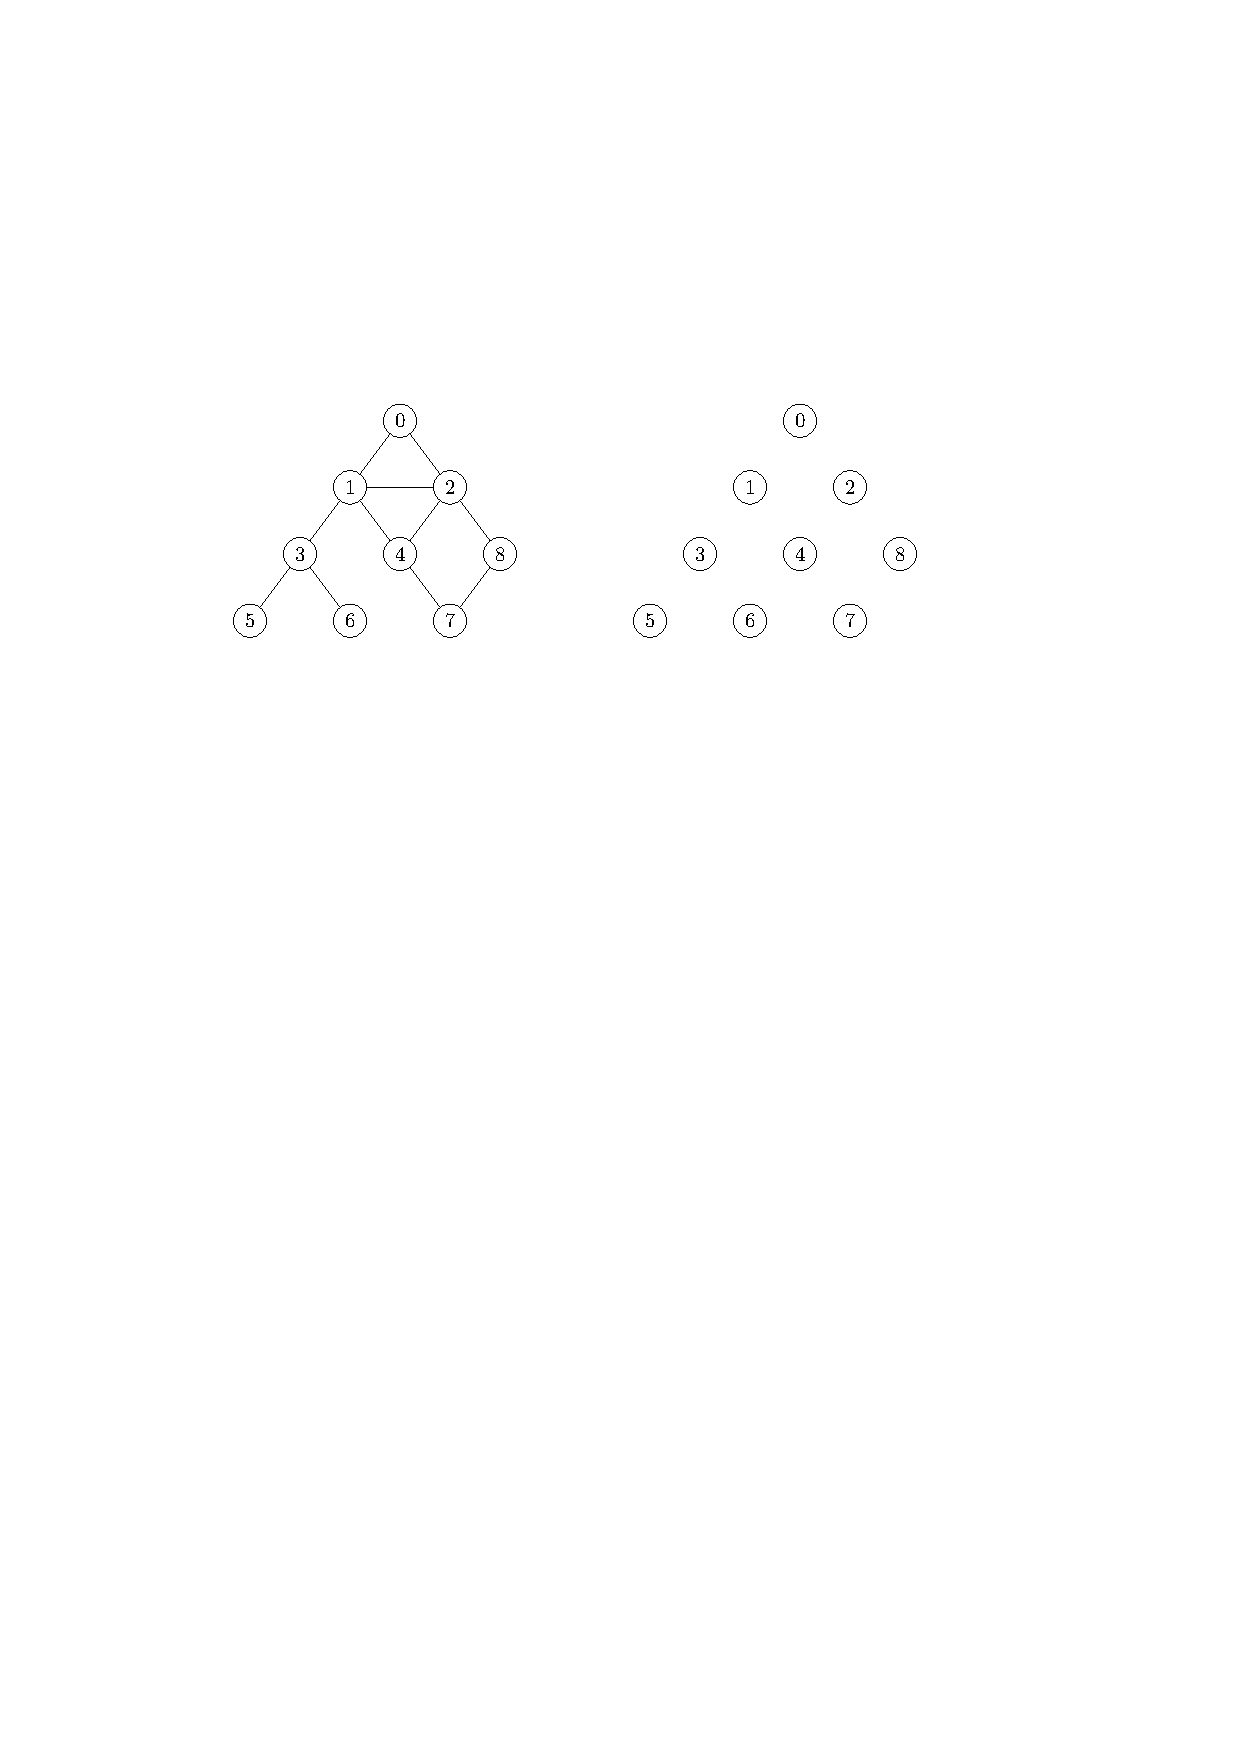
\includegraphics{TraverseGraphEx}
\end{center}
Find a tree arc, cross arc, forward arc and back arc (or say if that type of arc does not exist for that traversal).
\end{Boxample}
 
\section{Pseudocode for breadth-first search} \label{sec:bfs}
The first-in first-out processing of the grey nodes in BFS is ideally handled by a queue. 
The pseudocode for \algfont{BFS} and \algfont{BFSvisit} is in \cref{alg:BFScode,alg:BFSvisitcode}.
The time\-stamps $\seen$ and $\done$ of DFS are of less use here. 
It is more useful to record the number of steps from the root in the array $d$.

\begin{algorithm}[H]
  \caption{Breadth-first search algorithm.}
    \label{alg:BFScode}
\begin{algorithmic}[1]
\Function{BFS}{digraph $G$}
	\State queue $Q$  
	\State array $\colour[0..n-1]$, $\pred[0..n-1]$, $d[0..n-1]$
	\For{$u \in V(G)$} 
		\State $\colour[u] \gets $ WHITE; $\pred[u] \gets $ \texttt{null}
	\EndFor
	\For{$s \in V(G)$} 
		\If{$\colour[s] = $ WHITE } 
			\State \texttt{BFSvisit}$(s)$
		\EndIf
	\EndFor
	\State \Return{$\pred, d$}
\EndFunction
\end{algorithmic}
\end{algorithm}

\begin{algorithm}[H]
  \caption{Breadth-first search visit algorithm.}
     \label{alg:BFSvisitcode}
  \begin{algorithmic}[1]
\Function{BFSvisit}{node $s$}
	\State $\colour[s] \gets $ GREY; $d[s] \gets 0$ 
	\State $Q$.\texttt{insert}$(s)$
	\While{\textbf{not} $Q$.\texttt{isEmpty}$()$}
		\State $u \gets Q$.\texttt{peek}$()$
		\For{each $v$ adjacent to $u$}
			\If{$\colour[v] = $ WHITE}
				\State $\colour[v] \gets $ GREY; $\pred[v] \gets u$; $d[v] \gets d[u]+1$
				\State $Q$.\texttt{insert}$(v)$
			\EndIf
		\EndFor
		\State $Q$.\texttt{delete}$()$
		\State $\colour[u] \gets $ BLACK
	\EndWhile
\EndFunction
\end{algorithmic}
\end{algorithm}

\begin{Boxample} \label{ex:BFSqueue}
BFS on a digraph.
\begin{center}
  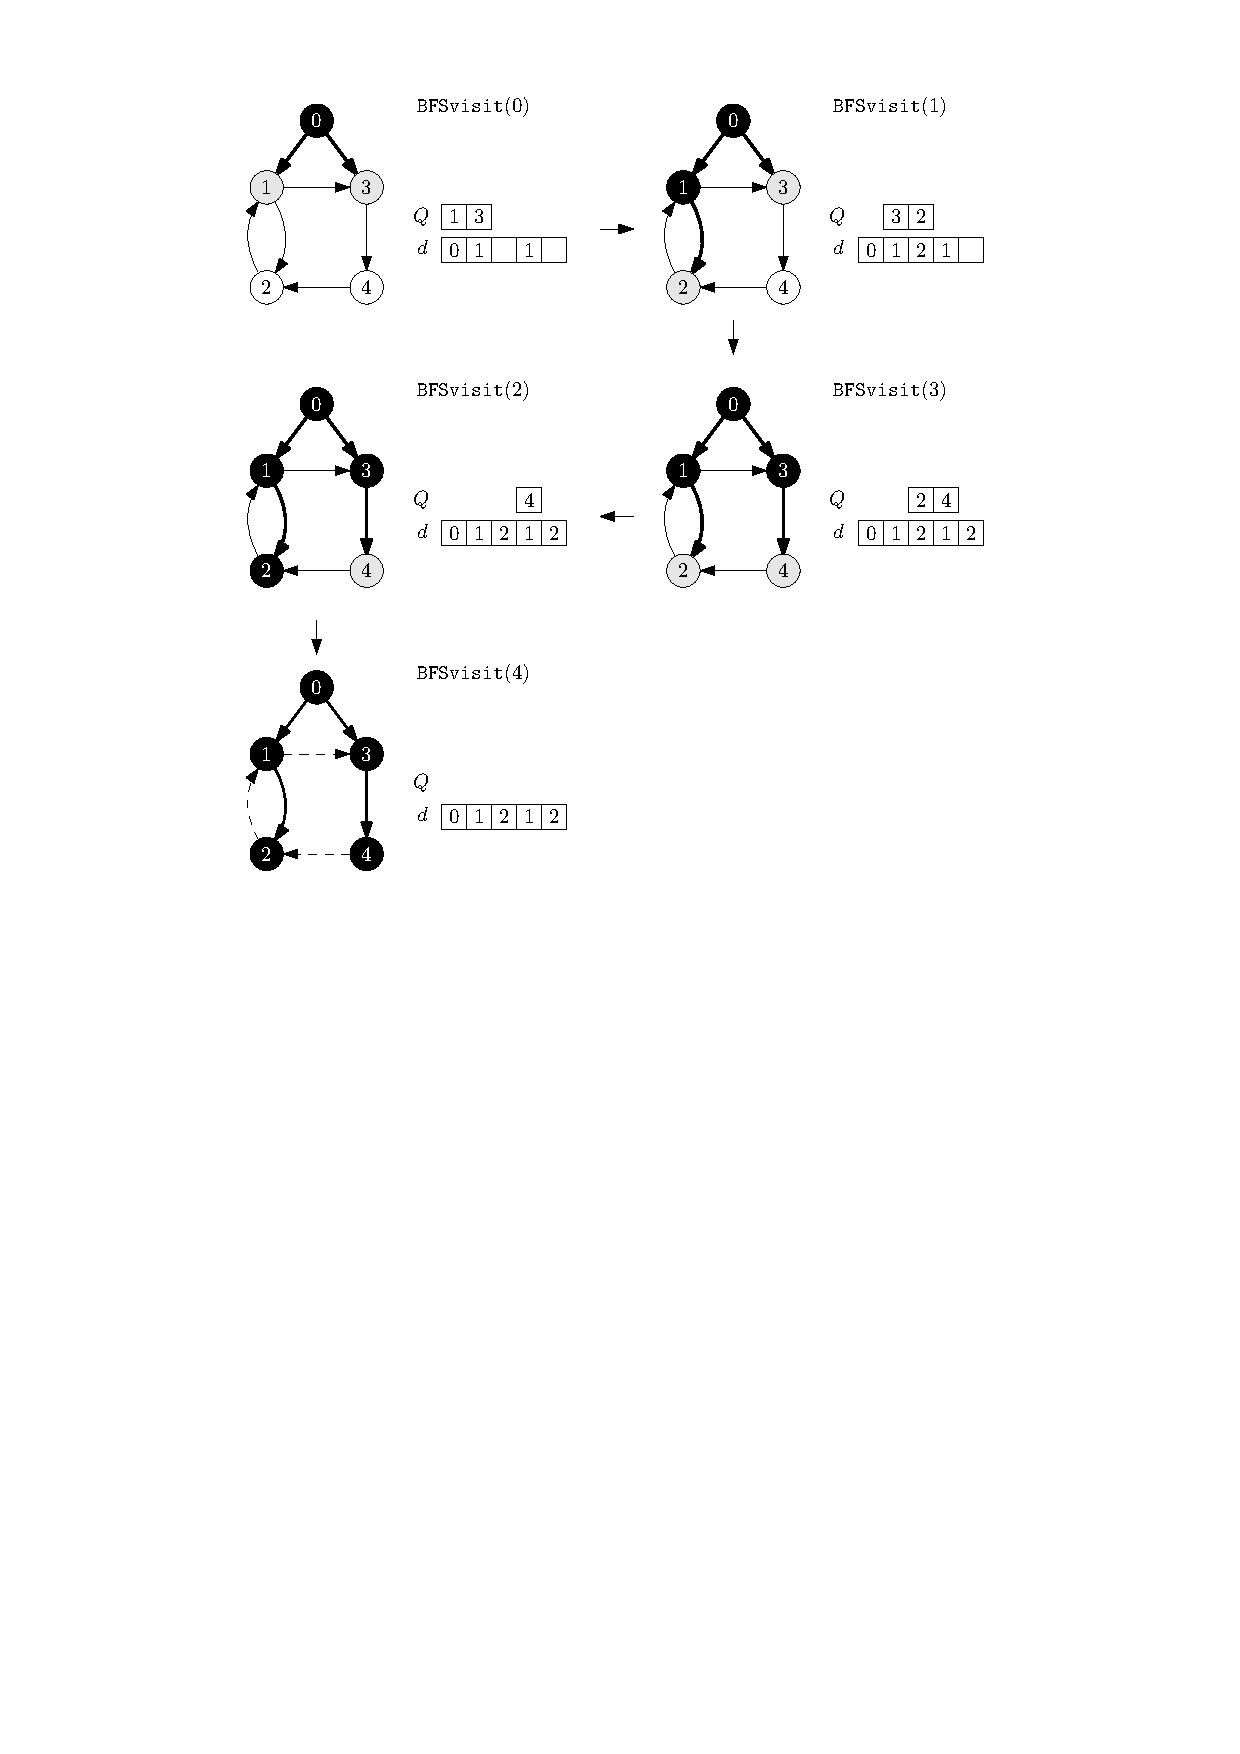
\includegraphics{BFSalgoQueue2}
\end{center}
\end{Boxample}

\begin{Boxample}
Execute BFS and following \cref{ex:BFSqueue} fill out the values for $Q$ and $d$, and highlight the BFS search tree after each step. 
\begin{center}
  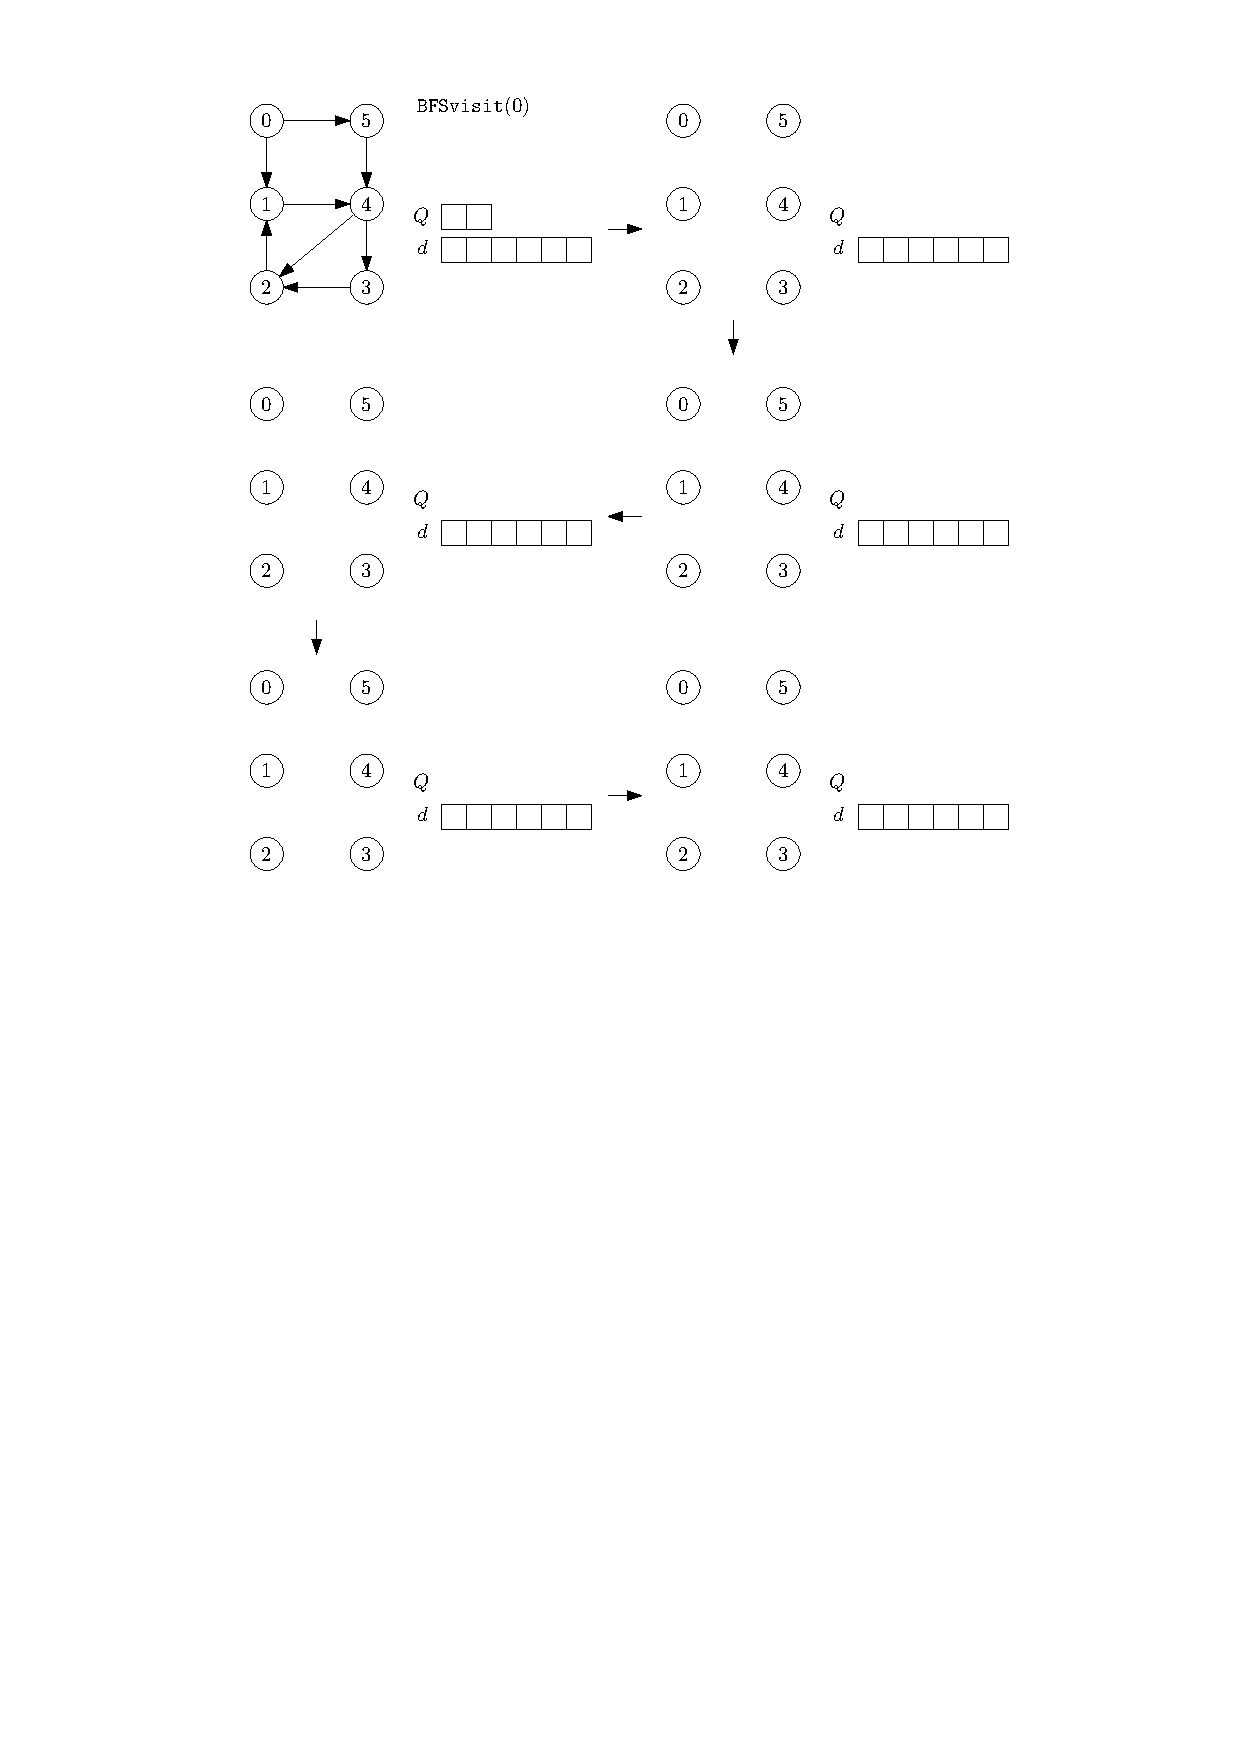
\includegraphics{BFSalgoQueueEx}
\end{center}
\end{Boxample}

\section{BFS useful results and facts} 
It is rather obvious that BFS processes all nodes at distance 1, then
all nodes at distance 2, etc, from the root. 
The formal theorem stating this is given below without proof (see book for a simple inductive proof).

\begin{Theorem} \label{thm:BFSdist}
Suppose we run \texttt{BFS} on a digraph $G$.
Let $v \in V(G)$, and let $r$ be the root of the search tree containing $v$. 
Then $d[v] = d(r, v)$.
\end{Theorem}

We can classify arcs, but the answer is not as nice as with DFS.

\begin{Theorem} \label{thm:BFS-arcclass}
Suppose that we are performing \texttt{BFS} on a digraph $G$. Let $(v,
w)\in E(G)$ and suppose that we have just chosen the grey node $v$. 
Then
\begin{itemize}
  \item if $(v, w)$ is a tree arc then $\colour[w] = $ WHITE, $d[w] = d[v] + 1$;
  \item if $(v, w)$ is a back arc, then $\colour[w] = $ BLACK, $d[w] \leq d[v] - 1$;  
  \item there are no forward arcs; and
  \item if $(v, w)$ is a cross arc then one of the following holds:
  \begin{itemize}
	\item $d[w] < d[v] - 1$, and $\colour[w] = $ BLACK;
	\item $d[w] = d[v]$, and $\colour[w] = $ GREY;
	\item $d[w] = d[v]$, and $\colour[w] = $ BLACK;
	\item $d[w] = d[v] - 1$, and $\colour[w] = $ GREY;
	\item $d[w] = d[v] - 1$, and $\colour[w] = $ BLACK.
  \end{itemize}
\end{itemize}
\end{Theorem}

\begin{Boxample}[6]
Explain why there are no forward arcs when performing BFS on a digraph.
\end{Boxample}

%\begin{proof}
%The arc is added to the tree if and only if $w$ is white. If the arc is
%a back arc, then $w$ is an ancestor of $v$; the FIFO queue structure
%means $w$ is black before the adjacency list of $v$ is scanned. 
%
%Now suppose that $(x, u)$ is a forward arc. Then since $u$ is a
%descendant of $x$ but not a child in the search forest, 
%Theorem~\ref{thm:BFSdist} yields $d[u]
%\geq d[x] + 2$. But by the last theorem we have $d[u] = d(s, u) \leq
%d(s, x) + 1 = d[x] + 1$, a contradiction. Hence no such arc exists.
%
%A cross arc may join two nodes on the same level, jump up one level,
%or jump up more than one level. In the last case, $w$ is already black
%before $v$ is seen. In the second case, $w$ may be seen before $v$,
%in which case it is black before $v$ is seen (recall $w$ is not the
%parent of $v$), or it may be seen after $v$, in which case it is grey
%when $(v, w)$ is explored. In the first case, $w$ may be seen before $v$ (in
%which case it is black before $v$ is seen), or $w$ may be seen after $v$
%(in which case it is grey when $(v, w)$ is explored).
%\end{proof}

In the special case of graphs we can say more.

\begin{Theorem} \label{thm:BFS-grapharcclass}
Suppose that we have performed \texttt{BFS} on a graph $G$. 
Let $\{v, w\}\in E(G)$. Then exactly one of the following conditions holds.
\begin{itemize}
	\item $\{v, w\}$ is a tree edge, $| d[w] - d[v] |= 1$;
	\item $\{v, w\}$ is a cross edge, $d[w] = d[v]$;
	\item $\{v, w\}$ is a cross edge, $| d[w] - d[v] | = 1$.
\end{itemize}
\end{Theorem}
%\begin{proof} By Theorem~\ref{thm:BFS-arcclass} there can be no forward
%edges, hence no back edges. A cross edge may not jump up more than
%one level, else it would also jump down more than one level, which is
%impossible by Theorem~\ref{thm:BFSdist}.
%\end{proof}

% For a given BFS tree, we can uniquely label the vertices of a digraph based on the time they were first seen. 
% For the graph $G_1$ of \cref{fig:graphExample2}, we label vertex 0 with 1,
% vertices \set{1,2} with labels \set{2,3}, vertices \set{3,4,8} with labels \set{4,5,6}, 
% and the last vertex level \set{5,6,7} with labels \set{7,8,9}.  
% These are indicated in \cref{fig:graphEx2-BFS}.

\section{Priority-first search} \label{sec:PFS}
Priority-first search is a more general and sophisticated form of traversal that encompasses both BFS and DFS (and others). 

\begin{itemize}
	\item Each grey node has associated with it an integer \defnfont{key}. 
	\item The interpretation of the key is of a priority: 
	the smaller the key, the higher the priority. 
	\item The rule for choosing a new grey node is to choose one with the smallest key.  
	\item The key can either be assigned once when the node is first seen and then left unchanged, 
	or could be updated at other times. We concentrate on unchanging keys here.
	\item To mimic BFS, set the key for the node $v$ to be the time that $v$ turns grey. 
	It will always remain as the lowest key until it turns black.
	\item To mimic DFS, set the key for node $v$ to be $-\seen[v]$, 
	so that the most recently seen node has the lowest key
	\item The running time of PFS depends on how long it takes to find the minimum key value.
	\item The rules described here implemented using an array take $\Omega(n)$ to find the lowest key 
	so the algorithm is $\Theta(n^2)$. Contrast with with $\Theta(m+n)$ for standard traversal.
	\item PFS is best described via the priority queue ADT, 
	which has more efficient implementations than using a standard array.
\end{itemize}

%In the simplest form of PFS, the key value is assigned when the node
%becomes grey, and never updated subsequently. More generally, the key
%may be further updated at other times. We shall see both types in this
%book. The second type of PFS is used in optimization problems as we
%shall discuss in Chapter~\ref{ch:weighted}. 
%
%The first type of PFS includes both BFS and DFS. In BFS, the key
%value of $v$ can be taken as the time $v$ was first coloured grey.
%Note that this means that a given grey node can be selected many
%times---until it becomes black, in fact, it will always have minimum
%key among the grey nodes. By contrast, in DFS we can take the key
%value to be $-\seen[v]$. Then the last node seen always has minimum
%key. It cannot be chosen again until the nodes seen after it have
%become black.
%
%The running time of PFS depends mostly on how long it takes to find the
%minimum key value, and how long it takes to update the key values.
%
%In the array implementation mentioned above, finding the minimum key
%value takes time of order $n$ at each step, so the quantity $a$ is
%$\Omega(n)$. Thus a PFS of this type will take time in $\Omega(n^2)$.
%This is worse than the $\Theta(n+m)$ we obtain with BFS and DFS using
%adjacency lists and a queue or stack respectively. One reason is that a
%simple array is not a particularly good data structure for finding the
%minimum key. You have already seen a better one in Part I of this 
%book---the binary heap. In fact PFS is best described via the priority
%queue ADT (see Section~\ref{sec:app:adt-informal}).

Pseudocode \algfont{PFS} and \algfont{PFSvisit} demonstrating the PFS is presented in \cref{alg:PFScode,alg:PFScodeVisit}. 
The subroutine \algfont{setKey} there is the rule for giving the key value when a node is inserted. 
We do not include any code for \texttt{setKey}.

\begin{algorithm}[H]
  \caption{Priority-first search algorithm (first kind)}
  \label{alg:PFScode}
\begin{algorithmic}[1]
\Function{PFS}{digraph $G$}
	\State priority queue $Q$  
	\State array $\colour[0..n-1]$, $\pred[0..n-1]$
	\For{$u \in V(G)$} 
		\State $\colour[u] \gets $ WHITE; $\pred[u] \gets $ \texttt{null}
	\EndFor
	\For{$s \in V(G)$} 
		\If{$\colour[s] = $ WHITE } 
			\State \texttt{PFSvisit}$(s)$
		\EndIf
	\EndFor
	\State \Return{$\pred$}
\EndFunction
\end{algorithmic}
\end{algorithm}

\begin{algorithm}[H]
  \caption{Priority-first visit algorithm (first kind)}
  \label{alg:PFScodeVisit}
  \begin{algorithmic}[1]
\Function{PFSvisit}{node $s$}
	\State $\colour[s] \gets $ GREY 
	\State $Q$.\texttt{insert}$(s$, \texttt{setKey}$(s))$
	\While{\textbf{not} $Q$.\texttt{isEmpty}$()$}
		\State $u \gets Q$.\texttt{peek}$()$
		\If{$u$ has a neighbour $v$ with $\colour[v] = $ WHITE}
			\State $\colour[v] \gets $ GREY
			\State $Q$.\texttt{insert}$(v$, \texttt{setKey}$(v))$
		\Else
			\State $Q$.\texttt{delete}$()$
			\State $\colour[u] \gets$ BLACK
		\EndIf
	\EndWhile
\EndFunction
\end{algorithmic}
\end{algorithm}

\begin{Boxample}
Execute PFS on the graph below with the key for node $v$ is the degree of $v$. 
Start the traversal at vertex 0 and break ties by choosing the vertex with the lower index first.
In each step add one vertex and edge to the search tree. 
\begin{center}
  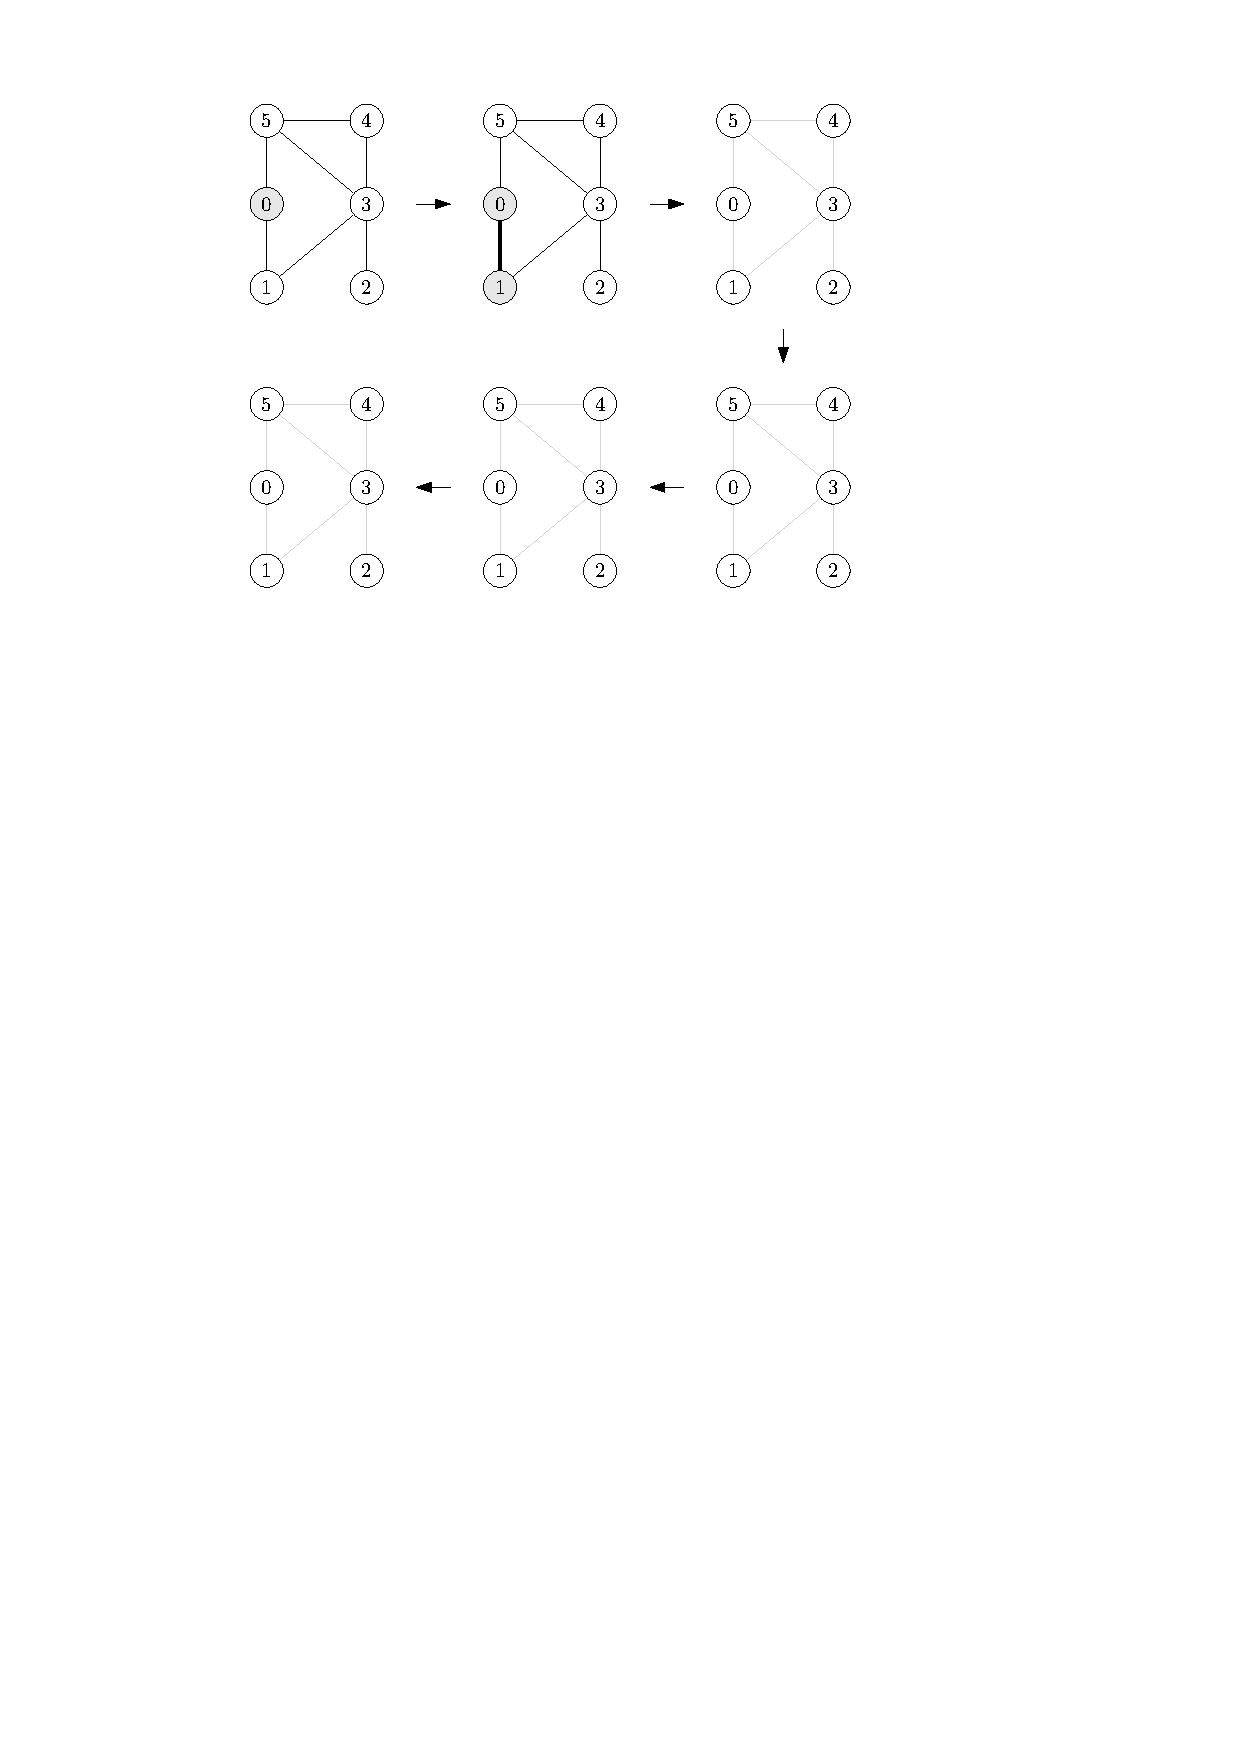
\includegraphics{PFSex}
\end{center}
\end{Boxample}

\chapter{Topological sort, acyclic graphs and girth} %------------------------
Many computer science applications require us to find precedence (or dependencies) among events. 
If we consider the events to be nodes and an arc $(u,v)$ means that $u$ precedes $v$, that is, 
that $u$ must be calculated before $v$ can be calculated, 
deciding the order in which to process events becomes a problem of sorting the nodes of a digraph.

\begin{Boxample}[0]
Consider a compiler evaluating sub-expressions of the expression $-(a+b) * (b+c) + ((b+c)+d)$.  
The compiler must compute, for example, (a+b) and (b+c) before it could compute $-(a+b) * (b+c)$. 
This can be shown as a dependency digraph where the arc $(u,v)$ means 
that $u$ depends on $v$ so that $v$ must be calculated first (this is the opposite of a precedence digraph discussed above).\\
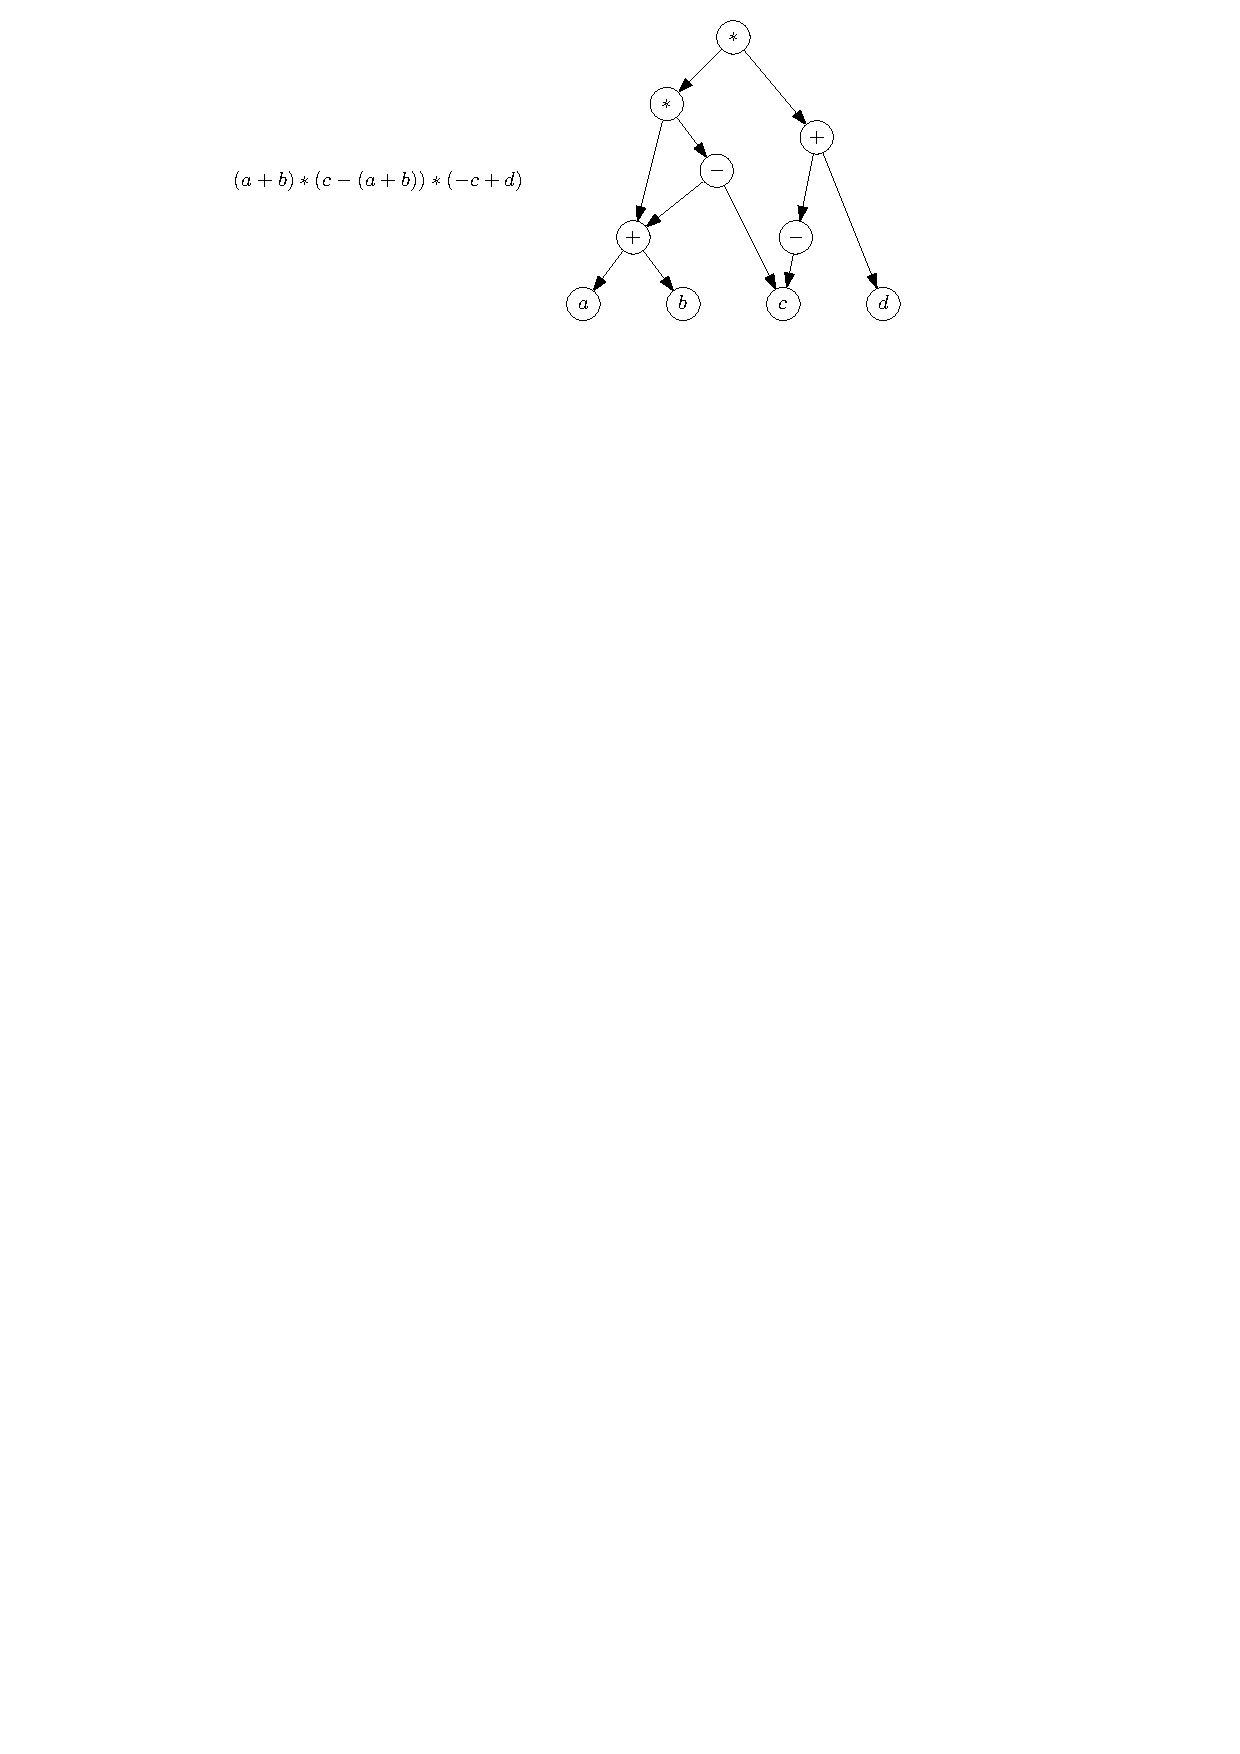
\includegraphics{precedence}
\end{Boxample}

Respecting all precedences/dependencies is equivalent to drawing the digraph 
with all nodes in a straight line and the arcs all pointing the same direction. 
The order of calculation starts at one end of the line and proceeds to the other.

\section{Topological sort}
\begin{Definition}
Let $G$ be a digraph. A \defnfont{topological sort} of $G$ is a linear
ordering of all its vertices such that if $G$ contains an arc $(u,v)$,
then $u$ appears before $v$ in the ordering. 
It is also known as a \defnfont{topological order} or \defnfont{linear order}.
\end{Definition}

For our arithmetic expression example above, a linear
order of the sub-expression digraph gives us an order (actually the reverse
of the order) where we can safely evaluate the expression.

\begin{Boxample}[0]
\label{ex:topoorders}
A graph with all possible topological orders and drawn with topological order $0, 1, 2, 3, 4$.  
Draw the graph for the topological order $0, 2, 1, 4, 3$. 
\begin{center}
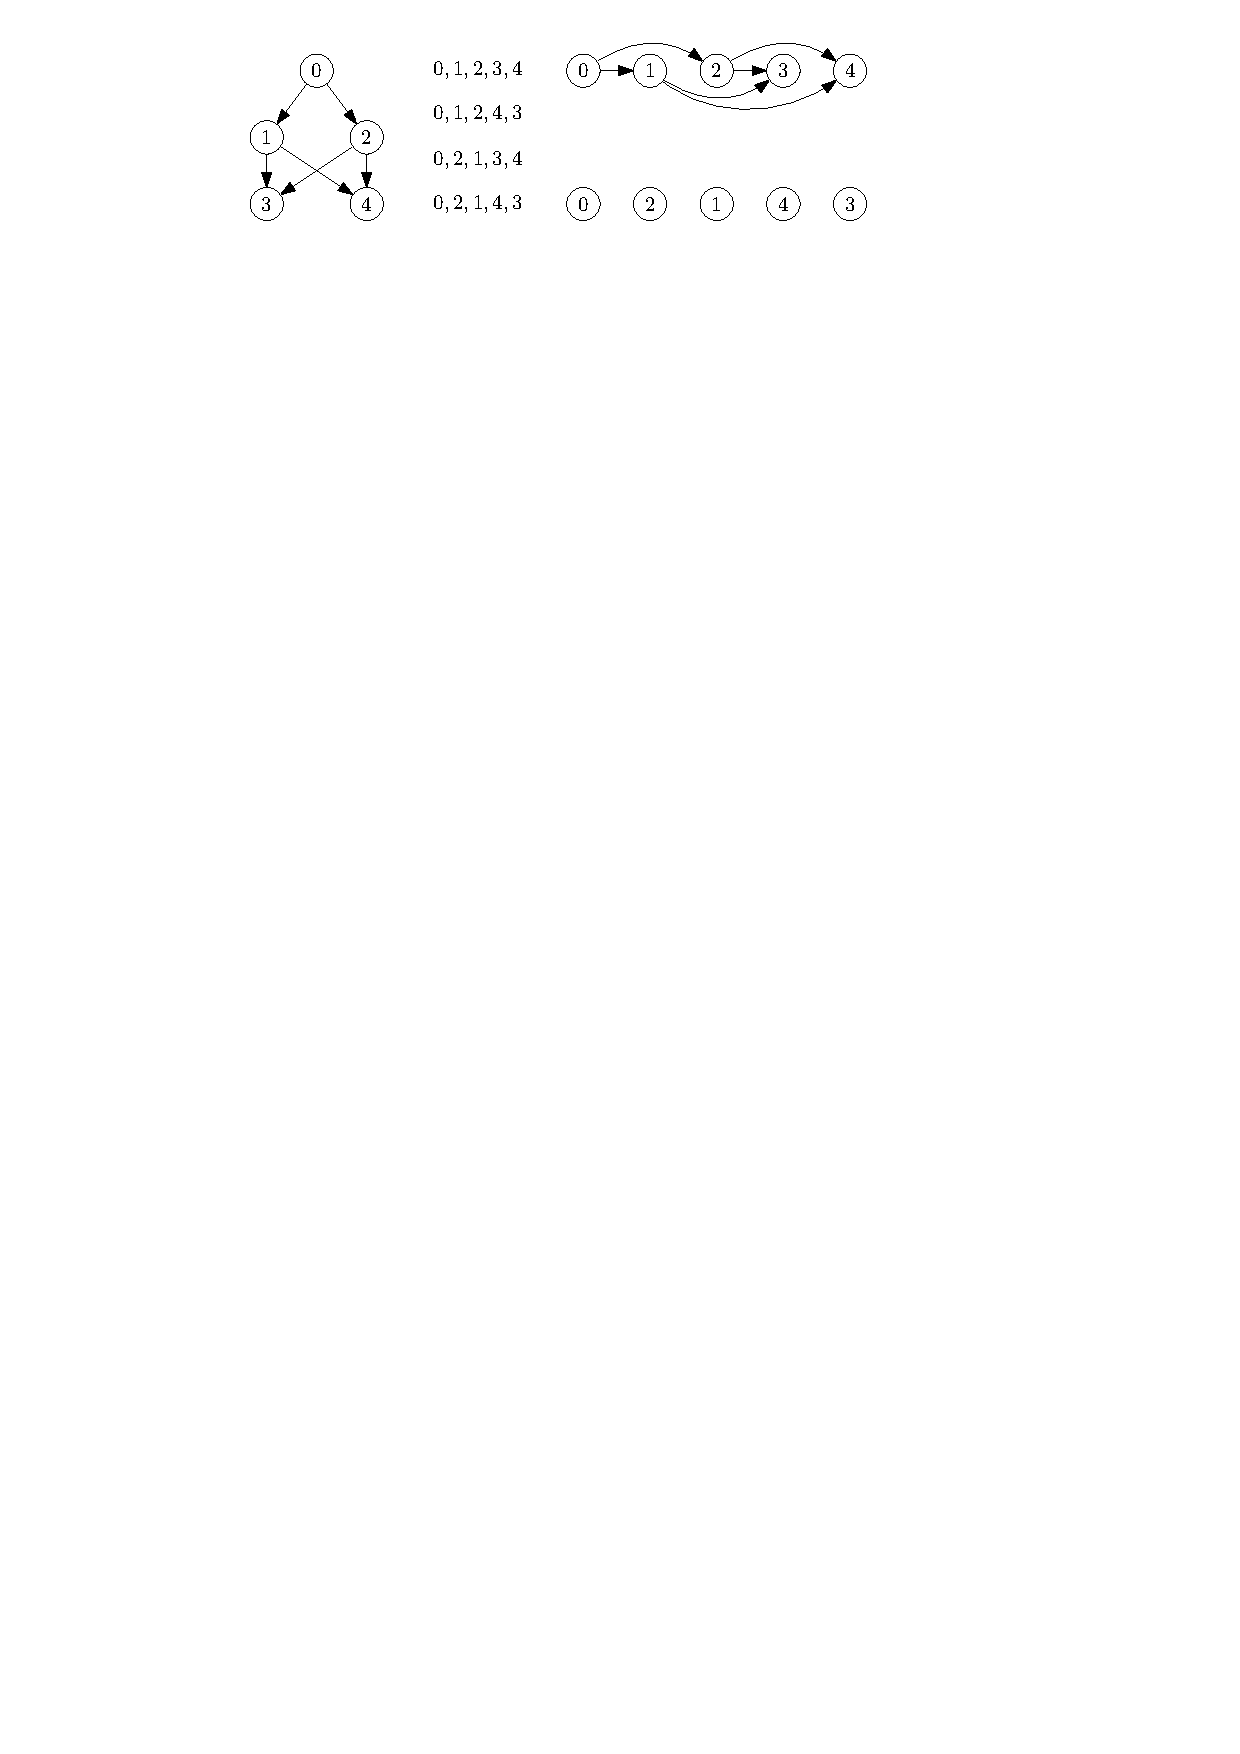
\includegraphics{topologicalOrder1}
\end{center}
Find a topological order of the following graph and draw it.
\begin{center}
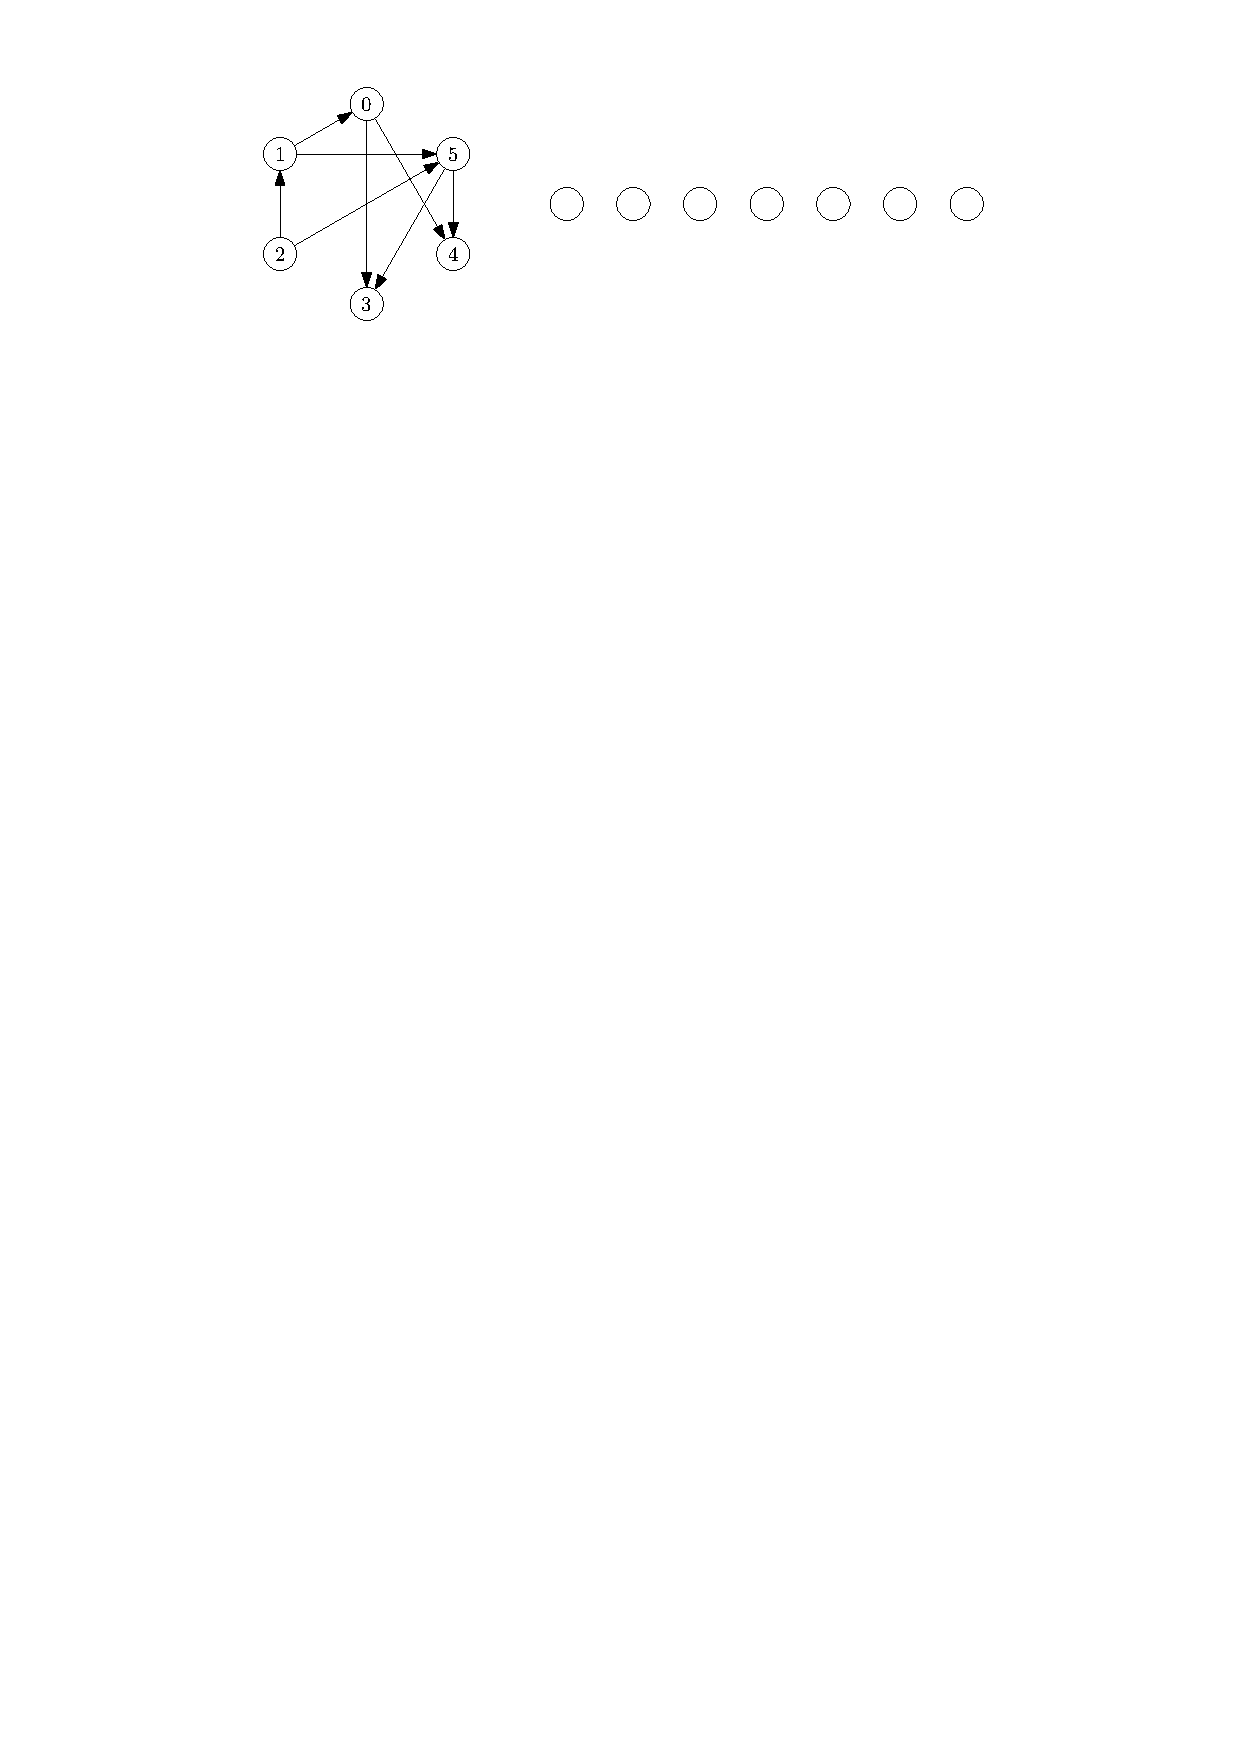
\includegraphics{topologicalOrder2}
\end{center}
Topological orders are not unique. List all possible topological orders of the following graph.
\begin{center}
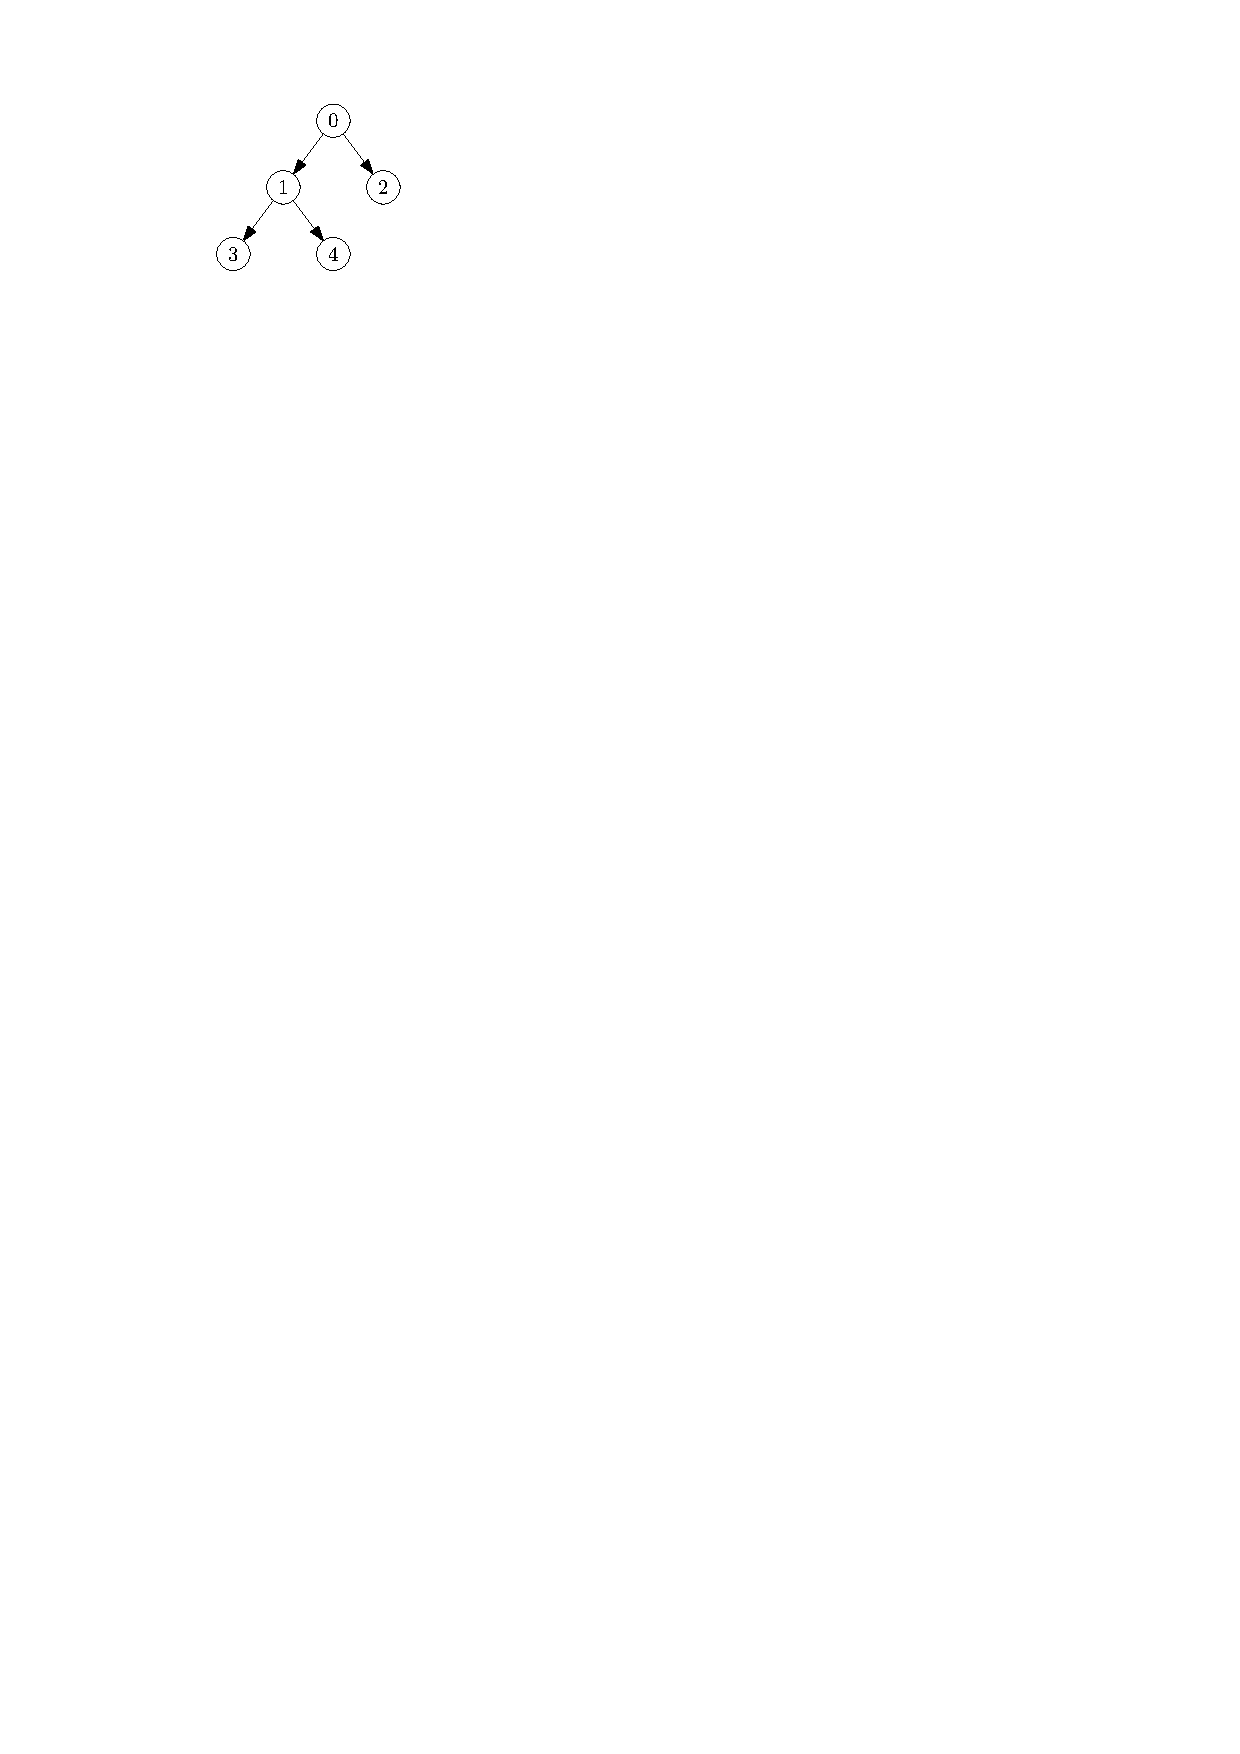
\includegraphics{topologicalOrder3}
\end{center}
\end{Boxample}

If the digraph contains a cycle, it is not possible to find
such a linear ordering. This corresponds to inconsistencies in the
precedences given (for example, $a$ precedes $b$ precedes $c$ precedes $a$) and no scheduling of the tasks is possible.

\begin{Definition}
A digraph without cycles is commonly called a \defnfont{DAG}, an
abbreviation for \textbf{d}irected \textbf{a}cyclic \textbf{g}raph.  
\end{Definition}

\begin{Theorem} \label{thm:topDAG}
A digraph has a topological order if and only if it is a DAG.
\end{Theorem}

\begin{Boxample}[8]
It is clear that if a digraph has a topological order it has no cycles, so it a DAG. 
Show that a DAG always has a topological order by first showing that every DAG has a source
and that by removing the source and any out-arcs from the source you still have a DAG. 
Show that the order in which nodes are removed gives a topological order.
\end{Boxample}

This theorem and proof then gives an algorithm \defnfont{zero-indegree sorting}
for topologically sorting a DAG. 
If we apply zero-indegree sorting to a digraph that is not a DAG, 
eventually it will stop because no source node can be found at some point.

\begin{Boxample}[3]
What is the running time of a naive implementation of zero-indegree where a zero degree node is found and then removed at each step? How could this idea be made more efficient?
\end{Boxample}

\section{Finding cycles and topological sorting using DFS}
DFS can be used to determine whether or not a digraph is a DAG and, if it is, find a topological sort.
\begin{itemize}
  \item Run DFS on $G$.
  \item If $G$ contains a cycle, the traversal will eventually reach a node that points to one that has been seen before. 
  In other words, we will detect a back arc. 
  \item If the traversal finds no back arcs, $G$ is a DAG 
  and the listing nodes in reverse order of DFS $\done$ times is a topological sort of $G$.
\end{itemize}

\begin{Theorem} \label{thm:findDAG}
Suppose that DFS is run on a digraph $G$. Then $G$ is acyclic if and only if there are no back arcs.
\end{Theorem}
%\begin{proof}
%Suppose that we run DFS on $G$. Note that if there is a
%back arc $(v, u)$, then $u$ and $v$ belong to the same tree $T$, with
%root $s$ say. Then there is a path from $s$ to $u$, and there is a path
%from $u$ to $v$ by definition of back arc. Adding the arc $(v, u)$ gives
%a cycle. 
%
%Conversely, if there is a cycle $v_0\, v_1\, \dots \, v_n\, v_0$, we may
%suppose without loss of generality that $v_0$ is the first node of the
%cycle  visited by the DFS algorithm. We claim that $(v_n, v_0)$ is a
%back arc. To see why this is true, first note that during the DFS $v_0$ is 
%linked to $v_n$ via a path of unvisited nodes (possibly of length shorter 
%than $n$).  We have $v_n$ as a descendant of $v_0$ in the DFS tree and
%a back arc $(v_n, v_0)$.
%\end{proof}

\begin{Theorem}
Let $G$ be a DAG. Then listing the nodes in reverse order of DFS
finishing times yields a topological order of $G$.
\end{Theorem}
\begin{proof} 
Consider any arc $(u,v) \in E(G)$. 
Since $G$ is a DAG, the arc is not a back arc by \cref{thm:findDAG}. 
In the other three cases, \cref{ex:DFS-arc-class} shows that $\done[u] > \done[v]$,
which means $u$ comes before $v$ in the alleged topological order.
\end{proof}

%Note that printing the nodes in order of finishing time gives a topological order of the reverse digraph $G_r$.



\begin{Boxample}[1] 
Find the topological order for the graph shown by running DFS starting at node $0$.  
Is it the same order you produced for this graph in \cref{ex:topoorders}?
\begin{center}
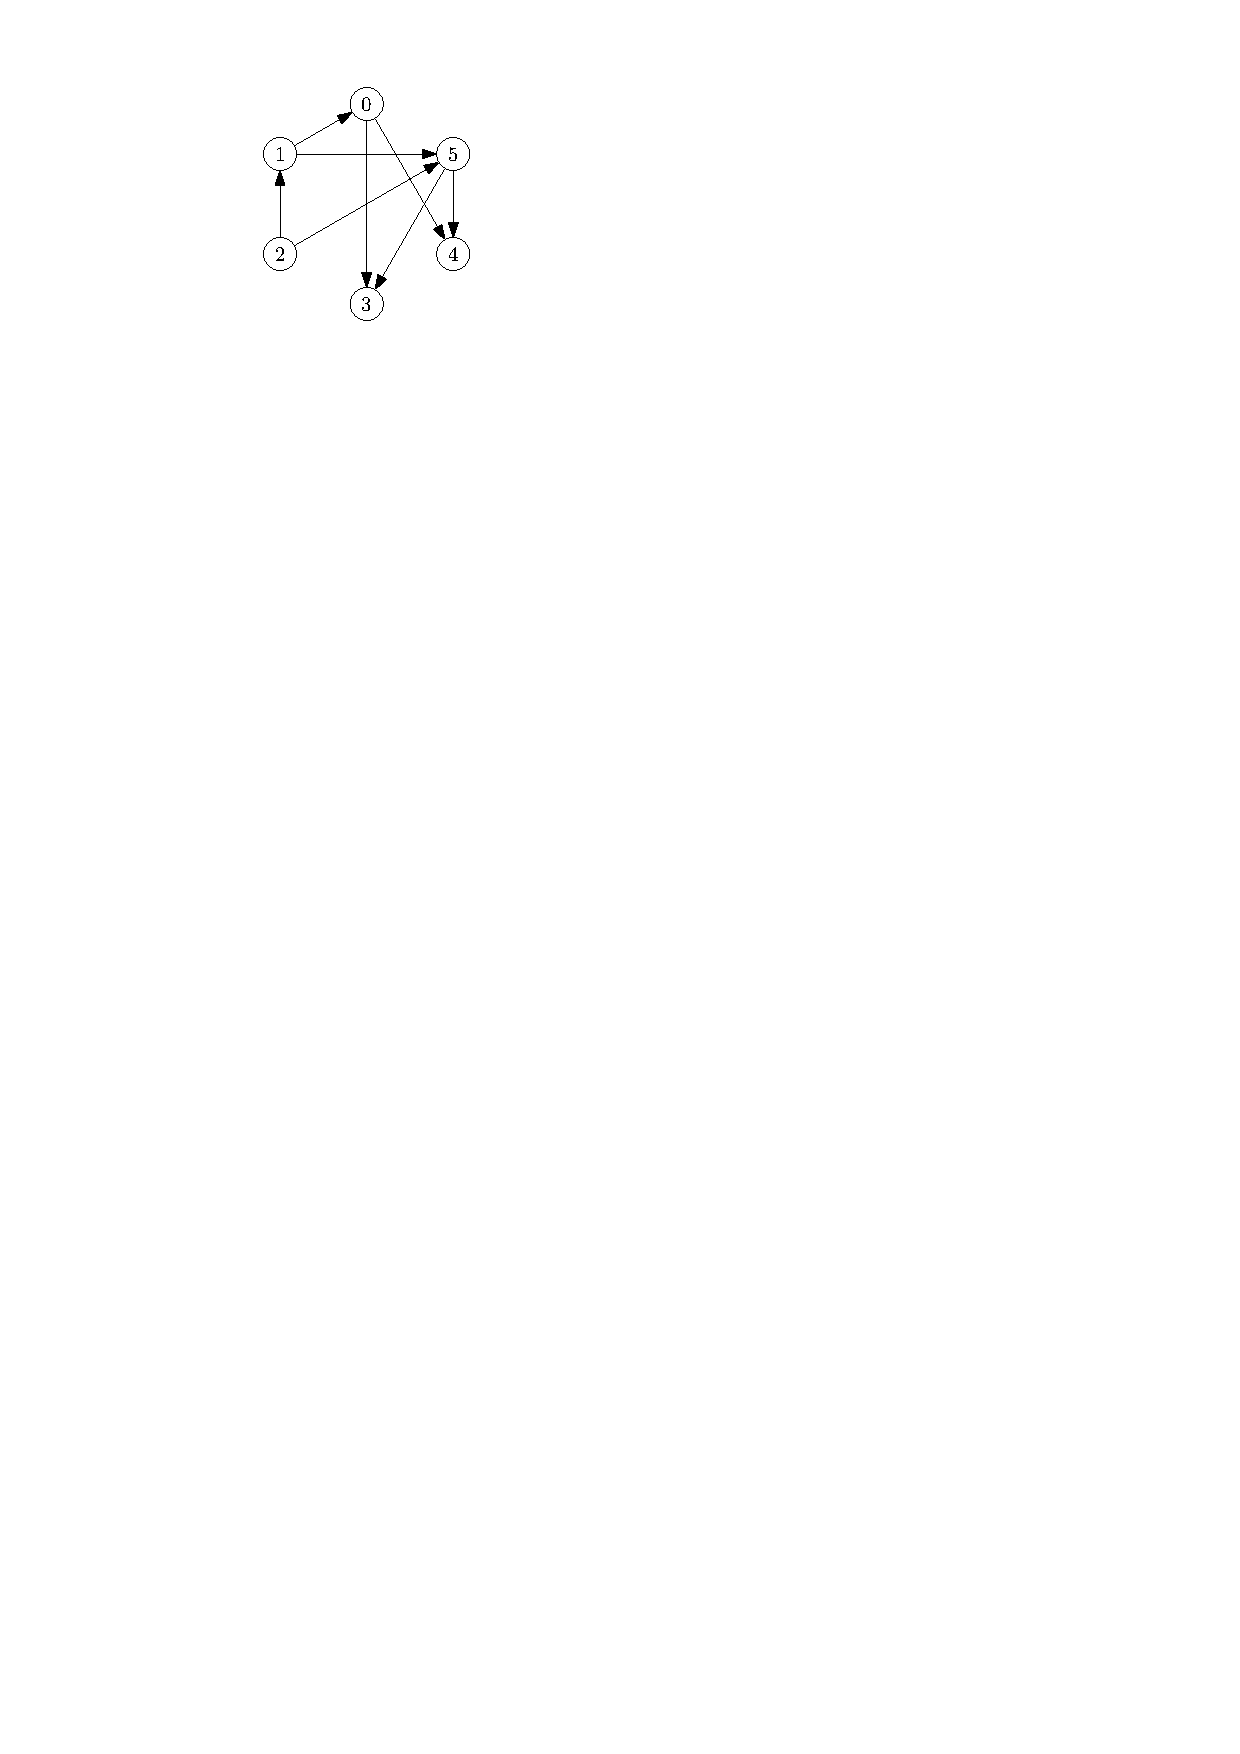
\includegraphics{topologicalOrder2b}
\end{center}
\end{Boxample}

%\begin{Boxample} \label{ex:sillytopsort}
%Show that the following method for topologically sorting a DAG does not work in 
%general: print the nodes in order of visiting time.
%\end{Boxample}

%\begin{Boxample} \label{ex:profP}
%Professor P has the following information taped to his mirror, to help
%him to get dressed in the morning.
%
%Socks before shoes; underwear before trousers; trousers before belt;
%trousers before shoes; shirt before glasses; shirt before tie; tie
%before jacket; shirt before hat; shirt before belt.
%
%Find an acceptable order of dressing for Professor P.
%\end{Boxample}

%\begin{Boxample} \label{ex:forest}
%Let $G$ be a graph. There is an easy way to show that $G$ is acyclic.
%It is not hard to show (see Section~\ref{sec:app:trees}) that a graph $G$ is 
%acyclic if and only if $G$ is a forest, that is, a union of (free) trees.
%
%Give a simple way to check whether a graph $G$ is acyclic. Does the method 
%for finding a DAG given above work for acyclic graphs also?
%\end{Boxample}

\section{The girth of a graph} \label{sec:girth}
The length of the smallest cycle in a graph is an important quantity. 
For example, in a communication network, short cycles are often something to be
avoided because they can slow down message propagation.

\begin{Definition}
The \defnfont{girth} of the graph is the length of the shortest cycle. If the graph has no cycles then the
girth is undefined but may be viewed as $+\infty$. 

For a digraph we use the term girth for its underlying graph and the (maybe non-standard) term \defnfont{directed girth} for
the length of the smallest directed cycle.
\end{Definition}

\begin{Boxample}[0]
What are the girth and the directed girth of the following digraph?
\begin{center}
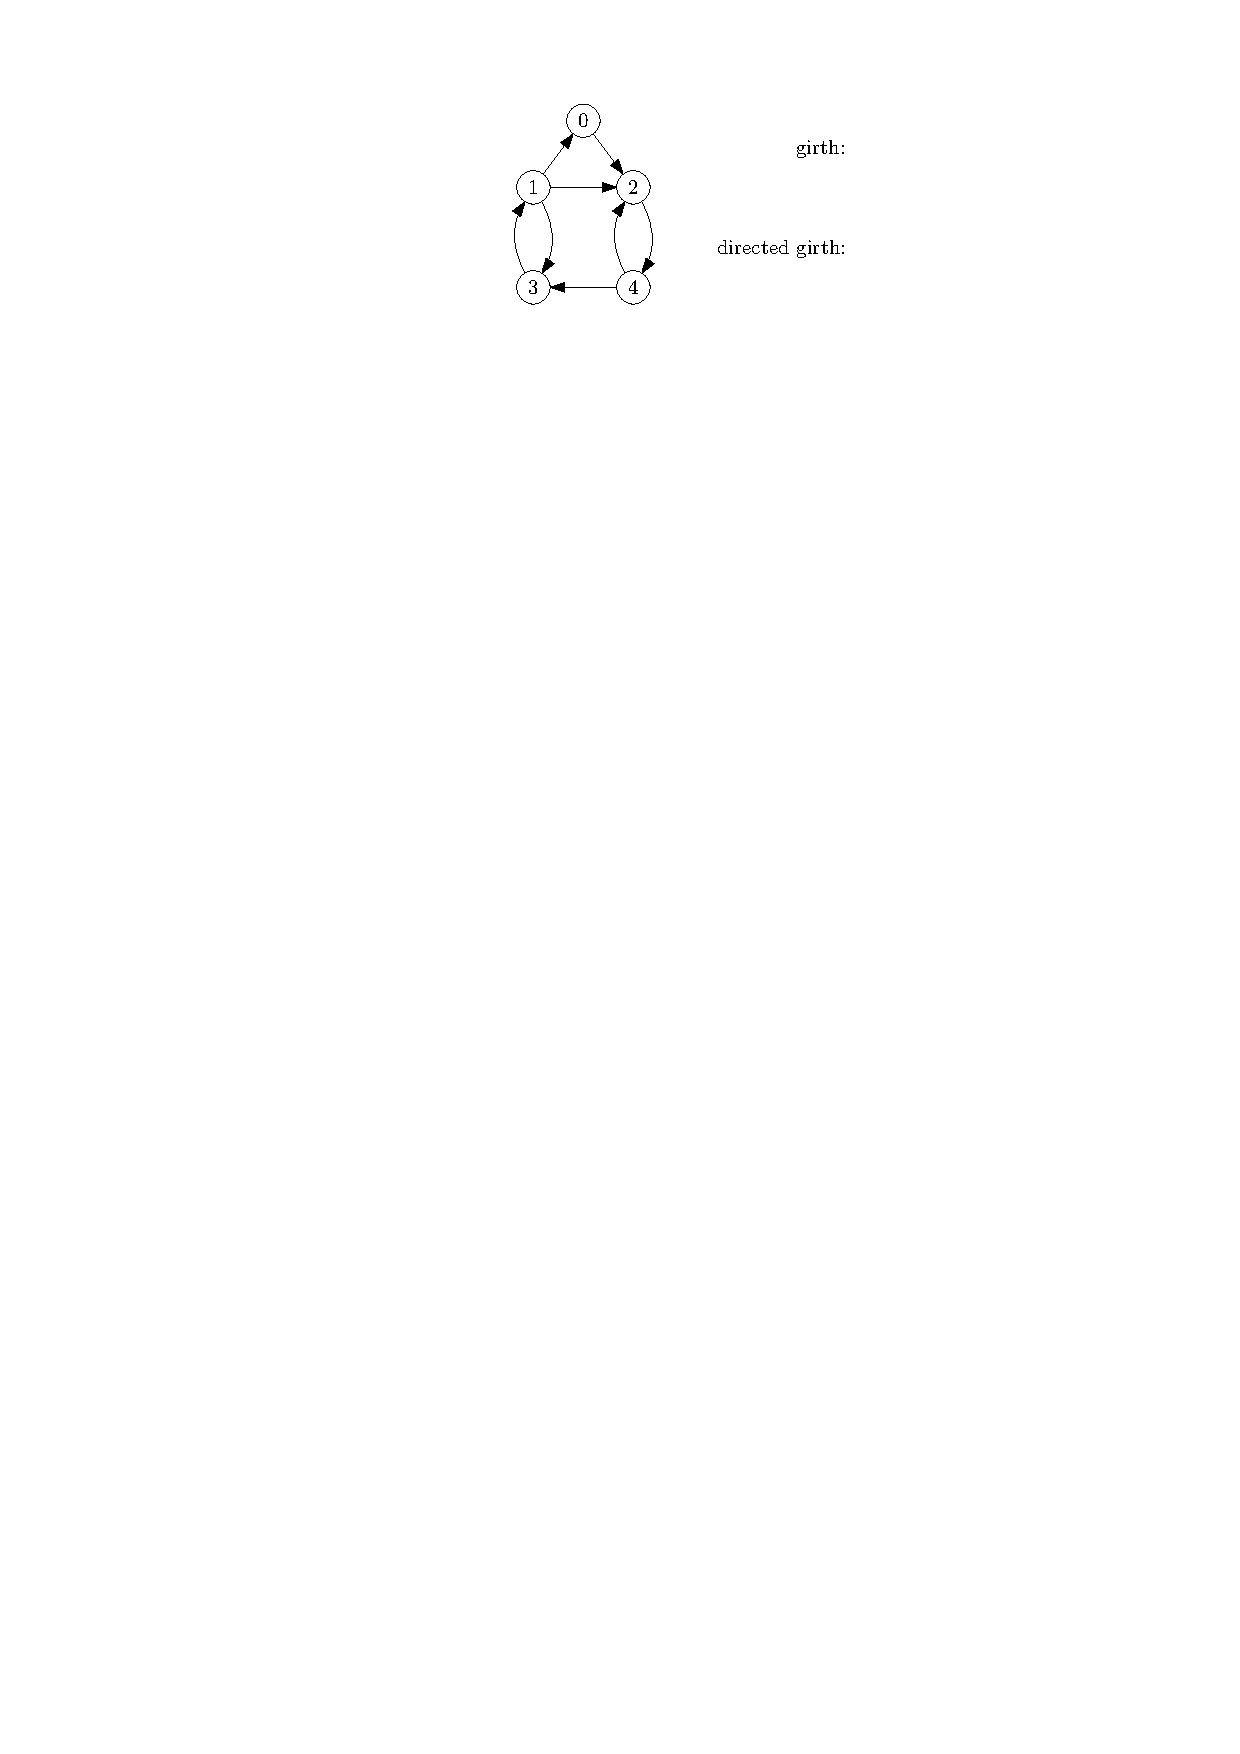
\includegraphics{girthEx}
\end{center}
\end{Boxample}




\chapter{Finding girth using BFS, connectivity, components, and strong components} %-----------------------

\section{Finding the girth of a graph with BFS}
How to compute the girth of a graph? Here is an algorithm for finding
the length of a shortest cycle containing a given vertex $v$ in a graph $G$. 
\begin{itemize}
  \item Perform \texttt{BFSvisit} starting at $v$. 
  \item If we meet a grey neighbour 
  (that is, we are exploring edge $\{x, y\}$ from $x$ and we find that $y$ is already grey), 
  continue only to the end of the current level and then stop.
  \item For each edge $\set{x, y}$ as above on this level, 
  if $v$ is the lowest common ancestor of $x$ and $y$ in the BFS tree, then there is a cycle
  containing $x, y, v$ of length $l=d(x) + d(y) + 1$. 
  \item Report the minimum value of $l$ obtained along the current level.
\end{itemize}

\begin{Boxample}[7] \label{ex:BFS-cycle} 
Prove above algorithm is correct by showing that:
\begin{enumerate}
\item meeting a grey neighbour means that you have indeed found a cycle;
\item any cycle that exists will be found in such a way; and 
\item the cycle found in this way will be the shortest going through $v$.
\end{enumerate}

\end{Boxample}

To compute the girth of a graph, we can simply run the above algorithm
from each vertex in turn, and take the minimum cycle length achieved.

\begin{Boxample}
An easy-to-implement DFS idea may not work properly. 
Consider the DFS tree originating from vertex $0$ of the graph below. 
Which is the smallest cycle it finds with the back edges? Which smaller cycle does it miss?
\begin{center}
  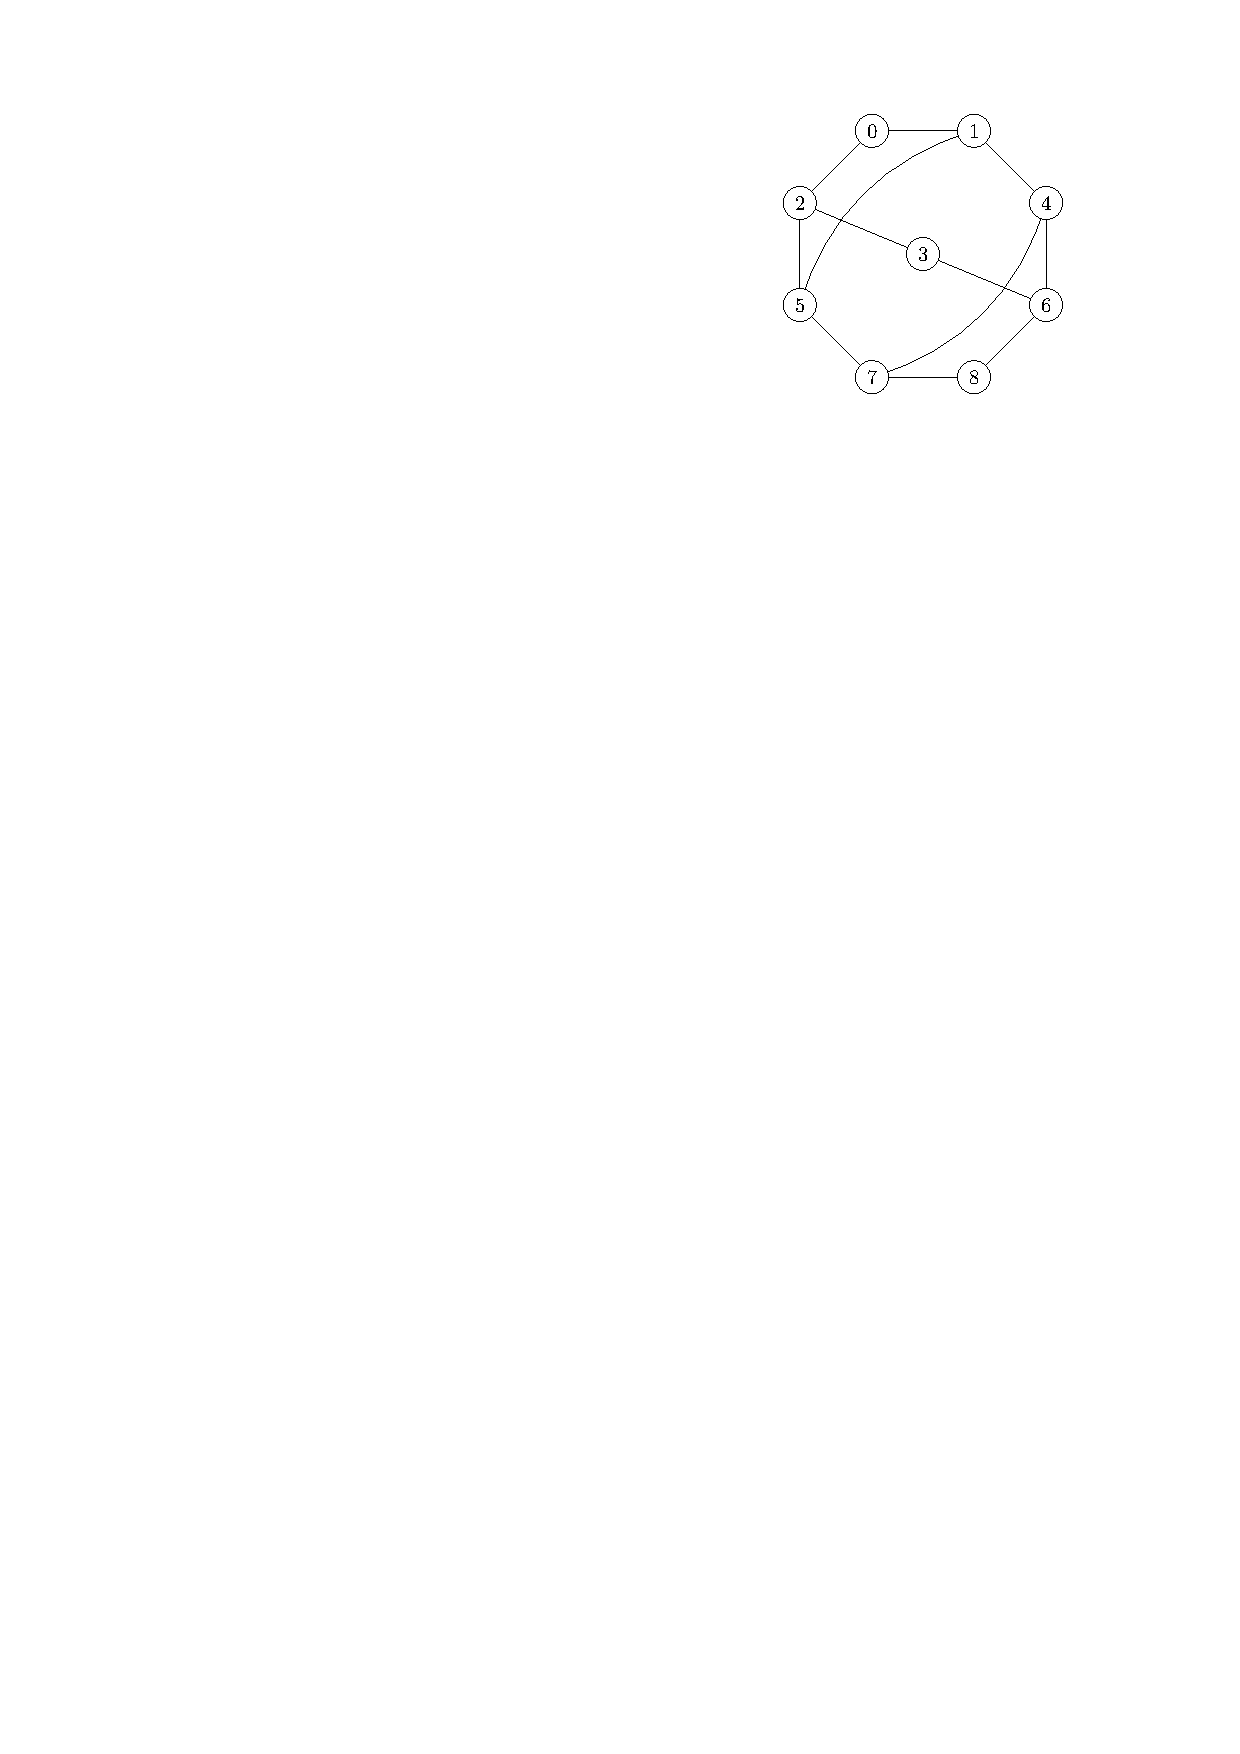
\includegraphics{girthEx2}
\end{center}
\end{Boxample}

% \begin{Boxample} \label{ex:shortest-cycle-thm}
% Give an example to show that in the shortest cycle algorithm, if we
% do not continue to the end of the level, but terminate when the first
% cycle is found, we may find a cycle whose length is one more than the
% shortest possible.
% \end{Boxample}
% TODO: include this?

\section{Finding the directed girth of a digraph with DFS}

A similar idea can be applied to finding the directed girth of a digraph.

\begin{Boxample}[2.5]
Convince yourself the the following procedure finds the (length of the) shortest directed cycle through node $v$ in a digraph.
\begin{enumerate}
\item Run \algfont{DFSvisit} starting at node $v$.
\item Whenever a back-arc of the form $(x,v)$ is found, we have found a cycle of length equal to $(1 + \mbox{the depth of }x\mbox{ in the search tree})$. 
\item When  \algfont{DFSvisit} completes, return the shortest length found.\\

\vspace{2.5cm}
How can this be used to find the directed girth of the digraph? What is the running time for doing so?
\end{enumerate}
\end{Boxample}

\section{Connectivity in graphs}
%For many purposes it is useful to know whether a digraph is ``all in one
%piece", and if not, to decompose it into pieces. We now formalize these
%notions. The situation for graphs is easier than that for digraphs.

For many purposes it is useful to know whether a digraph is ``all in one
piece", and if not, to decompose it into pieces.


\begin{Definition} 
A graph is \defnfont{connected} if for each pair of 
vertices $u, v \in V(G)$, there is a path between them.
\end{Definition}

\begin{Theorem} \label{thm:components}
Let $G$ be a graph. Then $G$ can be uniquely written as a union of
subgraphs $G_i$ with the following properties:
\begin{itemize}
  \item each $G_i$ is connected,
  \item if $i \neq j$, there are no edges from any vertices in $G_i$ 
  to any vertices in $G_j$.
\end{itemize}
\end{Theorem}
%\begin{proof}
%Consider the relation $\sim$ defined on $V(G)$, given by $u\sim v$ if
%and only if there is a path joining $u$ and $v$ (in other words, $u$ and
%$v$ are each reachable from the other). Then $\sim$ is an equivalence
%relation and so induces a partition of $V(G)$ into disjoint subsets. The
%subgraphs $G_i$ induced by these subsets have no edges joining them by
%definition of $\sim$, and each is connected by definition of $\sim$.
%\end{proof}

The subgraphs $G_i$ above are called the \defnfont{connected components} of the graph $G$. 
Clearly, a graph is connected if and only if it has exactly one connected component.

\begin{Boxample}[2] \label{eg:components}
The graph obtained by deleting two edges from a triangle has 2 connected components. Draw a graph with 5 vertices, 5 edges and 2 connected components.
\end{Boxample}

We can determine the connected components of a graph easily by using a
traversal algorithm. The following obvious theorem explains why.

\begin{Theorem} \label{thm:trav-comps}
Let $G$ be a graph and suppose that DFS or BFS is run on $G$. Then the
connected components of $G$ are precisely the subgraphs spanned by the
trees in the search forest. 
\end{Theorem}

So to find the components of a graph $G$:
\begin{itemize}
\item Run BFS or DFS on $G$ and count of the number of times we choose a root -- this is the number of components.
\item Store or print the vertices and edges in each component as we explore them.
\item This is a linear time algorithm, $O(m+n)$.
\end{itemize}

\section{Connectivity in digraphs}
The intuition of a digraph being ``all in one piece" is not as useful as it was for graphs. 

\begin{Boxample}[0]
This digraph appears to be ``all in one piece'' as its underlying graph is connected. 
But can you get from any node to any other node following the direction of the arcs?
\begin{center}
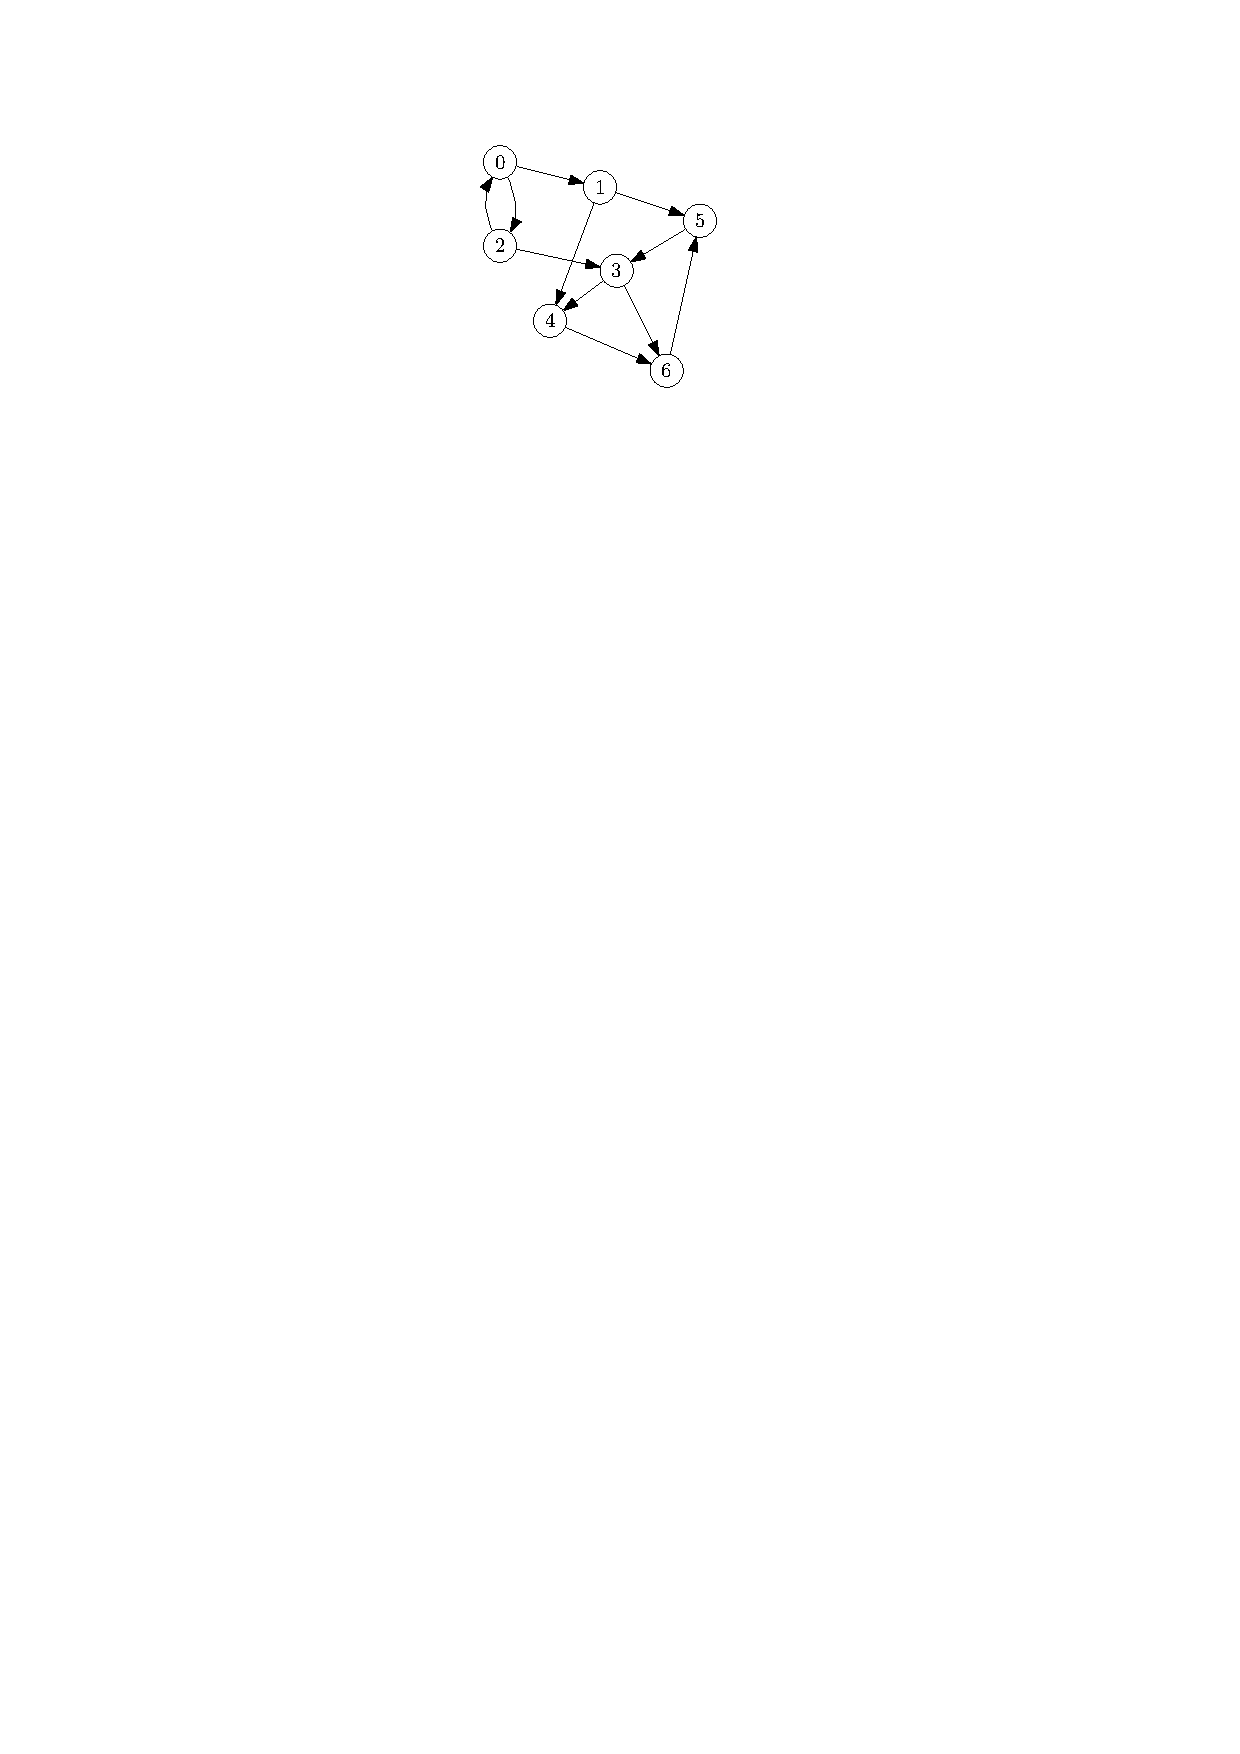
\includegraphics{connectedComponentDigraph}
\end{center}
\end{Boxample}

This example motivates the following definition.

\begin{Definition}
A digraph $G$ is \defnfont{strongly connected} if for each pair of nodes $u$, $v$ 
of $G$, there is a path in $G$ from $u$ to $v$ and from $v$ to $u$ (that is, $u$ and $v$ are reachable from one another).
\end{Definition}

\begin{Boxample}[4]
Show that a strongly connected digraph of order at least three contains at least one cycle.
% Note: Definition of cycle says cycle must contain at lesat three vertices, hence example with ``order at least two'' doesn't work.
\end{Boxample}

\begin{Definition} 
A \defnfont{strongly connected component}, $G_i$, of $G$ is a maximal sub-digraph of $G$ 
such that $G_i$ is strongly connected. 
All nodes of $G$ are in exactly one such $G_i$, so the partition into strongly connected components is unique.
\end{Definition}

%%\newpage
%\begin{Theorem}
%\label{thm:scc}
%Let $G=(V, E)$ be a digraph. Then $V$ can be uniquely written as a union of
%disjoint subsets $V_i$, with each corresponding induced subdigraph $G_i$ being
%a strongly connected component of $G$.
%\end{Theorem}
%
%\begin{proof} Consider the relation $\sim$ defined on $V$, given by
%$u\sim v$ if and only if there is a path joining $u$ and $v$ and a path
%joining $v$ and $u$ (in other words, $u$ and $v$ are each reachable
%from the other). Then $\sim$ is an equivalence relation and so induces
%a partition of $V$ into disjoint subsets.  By definition, each 
%subdigraph $G_i$ is strongly connected and of maximal order.
%\end{proof}

\begin{Boxample}[0]\label{eg:scc}
This digraph has three strongly connected components. Find and draw the two missing ones.\\

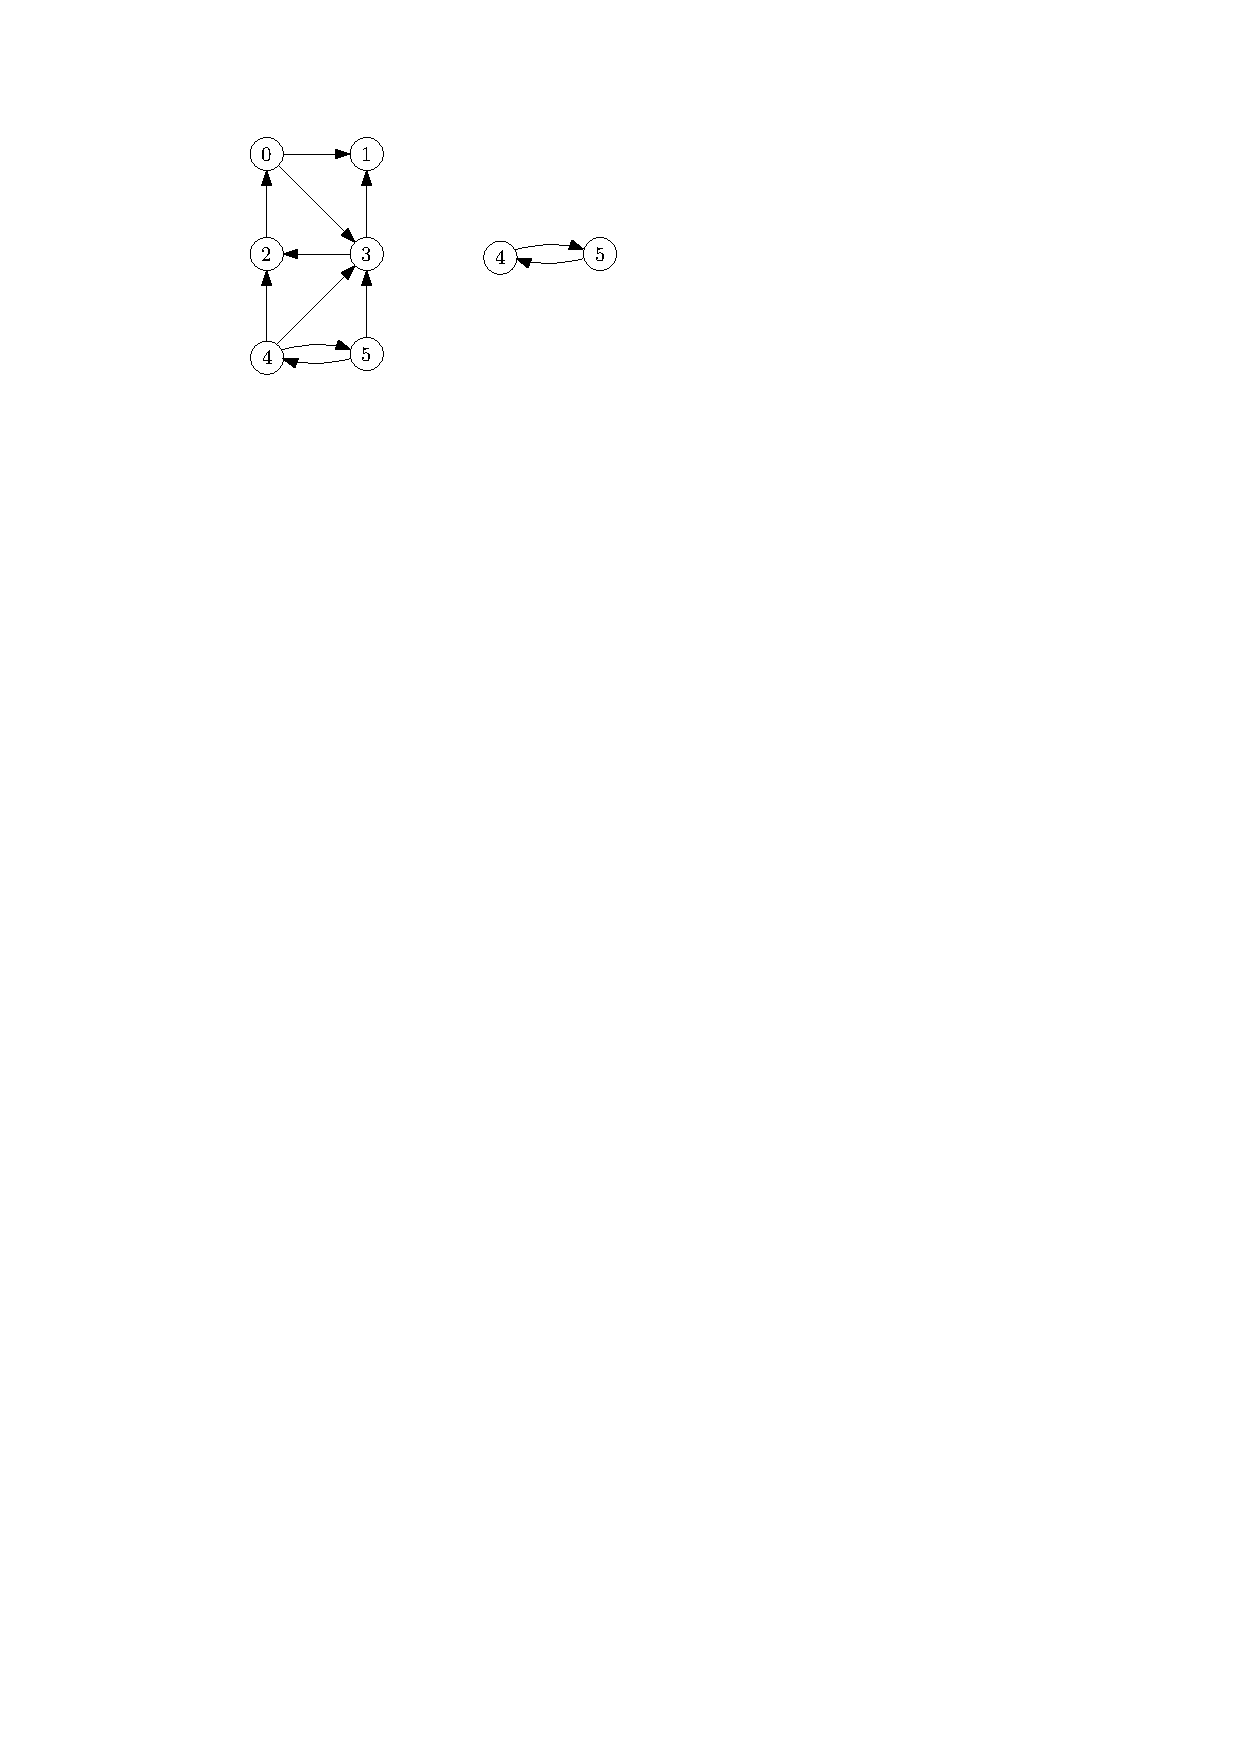
\includegraphics{SCCex}

Note that there are arcs of the digraph not included in the strongly connected components.
\end{Boxample}

\begin{Boxample}[4]
Find a counter-example to show that the method for finding connected components of graphs 
in \cref{thm:trav-comps} fails at finding strongly connected components of digraphs.
\end{Boxample}



%\subsection*{Exercises}
%
%\begin{Exercise}
%\label{ex:DFSfails}
%Give an example to show that a single use of DFS does not in general
%find the strongly connected components of a digraph.
%\end{Exercise}
%
%\begin{Exercise}
%\label{ex:dolinscc}
%Carry out the above  algorithm by hand on the digraph of
%\cref{eg:scc} and verify that the components given there are
%correct. Then run it again on the reverse digraph and verify that the
%answers are the same.
%\end{Exercise}


\chapter{Finding Strong components, bipartite graphs} %--------------------------------------------------

\section{Finding the strongly connected components}

%Note that if the underlying graph of $G$ is connected but $G$ is
%not strongly connected, then  there are strong components $C_1$ and
%$C_2$ such that it is possible to get from $C_1$ to $C_2$ but not
%from $C_2$ to $C_1$. If $C_1$ and $C_2$ are different strong
%components, then any arcs between them must either all point from
%$C_1$ to $C_2$ or from $C_2$ to $C_1$.  Suppose that we imagine
%each strong component shrunk to a single node (so we ignore the
%internal structure of each component, but keep the arcs between
%components). Then in the digraph resulting, if $v\neq w$ and we can
%get from $v$ to $w$ then we cannot get from $w$ to $v$. In other
%words, no pair of nodes can belong to a cycle, and hence the digraph
%is acyclic. See \cref{fig:sccdecomp}. Note that the converse
%is also true: if we have an acyclic digraph $G$ and replace each
%node by a strongly connected digraph, the strongly connected
%components of the resulting digraph are exactly those digraphs that
%we inserted.

%Note the similarity between this and the search forest decomposition
%in \cref{fig:travdecomp}. In that case, if we shrink each
%search tree to a point, the resulting digraph is also acyclic.


We can determine if $G$ is strongly connected or not (i.e., has a single strongly connected component) 
by running \texttt{BFSvisit} or \texttt{DFSvisit} originating from each node in turn. 
If it is strongly connected, all trees produced will span $G$. 
The running time of such an algorithm is $\Theta(n^2+nm)$.

{\color{red} TODO: compress and clarify this argument. OK to omit formal proof if decent intuition is given}

We can do better by using DFS more cleverly. 

Consider the reverse $G_r$. The strong components of $G_r$ are the
same as those of $G$. Shrinking each strong component to a point,
we obtain  acyclic digraphs $H$ and $H_r$. Consider a sink $S_1$ in
$H_r$. If we run DFS on $G_r$ starting  in the strong component
$S_1$, we will reach every node in that component \boldfont{and no
other nodes of $G_r$}. The DFS tree will exactly span $S_1$. Now
choose the next root to lie in the strong component $S_2$ node of
$H_r$ whose only possible out-neighbour is $S_1$ (this is possible
by the same reasoning used for zero-indegree sort, except here we
deal with outdegree). The DFS will visit all of $S_2$ and no other
nodes of $G_r$ because all other possible nodes have already been
visited. Proceed in this way until we have visited all strong
components.

We have shown that if we can choose the roots correctly, then we can
find all strong components. Now of course we do not know these components
\boldfont{a priori}, so how do we identify the roots to choose?

Whenever there is a choice for the root of a new search tree, it must
correspond to a new node of the DAG $H_r$. We want at least a reverse
topological order of $H_r$. This is simply a topological order for
$H$. Note that in the case where $H=G$ (each strong component has just
one point), then $G$ is a DAG. The method above will work if and only
if we choose the roots so that each tree in the DFS for $G_r$ has only
one point. We just need a topological order for $G$, so run DFS on $G$
and print the nodes in reverse order of finishing time. Then choose the
roots for the DFS on $G_r$ in the printed order.

It therefore seems reasonable to begin with a DFS of $G$. Furthermore,
an obvious choice is: in the DFS of $G_r$, \boldfont{choose each new root
from among white nodes that finished latest in $F$}.

Then each DFS tree in the search of $G_r$ definitely contains the strong
component $S$ of the root $r$. To see this, note that no node in that
strong component could have been visited before in $G_r$, otherwise $r$
would have already been visited. By \cref{thm:white-path}, every
node in the strong component of $r$ is a descendant of $r$.

The only thing that could go wrong is that a search tree in $G_r$
might contain more than one strong component. This cannot happen,
as we now prove.

\begin{Theorem} \label{thm:scc-alg} 
If the following rule for choosing roots is used in the algorithm
described above, then each tree in the second search forest spans a
strong component of $G$, and all strong components arise this way.

Rule: use the white node whose finishing time in $F$ was largest.
\end{Theorem}

%\begin{proof}
%Suppose that a search tree in $G_r$ does  contain more than one strong
%component. Let $S_1$ be the first strong component seen in $G_r$ and let
%$S_2$ be another, and let the roots be $r, s$ respectively. Note that by
%the rule for choosing nodes $r$ was the first node of $S_1$ seen in $F$
%(by Theorem~\ref{thm:white-path}, every node of $S_1$ is a descendant
%of the first one seen, which therefore has latest finishing time). The
%analogous statement holds for $s$ and $S_2$.
%
%By the rule for choosing roots, we have $\done[r] > \done[s]$ in $F$. We
%cannot have $\seen[s] > \seen[r]$ in $F$, for then $s$ would be a descendant
%of $r$ in $F$ and in $G_r$, so they would belong to the same strong
%component. Thus $\seen[r] > \seen[s]$ in $F$. Hence $S_2$ was explored
%in $F$ before $r$ (and hence any node of $S_1$) was seen. But then $r$
%would have been reachable from $s$ in $G$ via a path of white nodes,
%so Theorem~\ref{thm:white-path} shows that $r$ and $s$ are in the same
%strong component, another contradiction.
%\end{proof} 

The above algorithm runs in linear time with adjacency lists, since each
DFS and the creation of the reverse digraph take linear time. We only
need to remember  while performing the first DFS to store the nodes in
an array in order of finishing time. 

\section{Bipartite graphs}

Many graphs in applications have two different types of nodes, and no
relations between nodes of the same type (this is a model of sexually
reproducing organisms, for example).

\begin{Definition}
A graph $G$ is \defnfont{bipartite} if $V(G)$  can be partitioned into
two nonempty disjoint subsets $V_0, V_1$ such that each edge of $G$
has one endpoint in $V_0$ and one in $V_1$.
\end{Definition}

\begin{Boxample} \label{ex:bipartite}
This graph is bipartite.  
The isolated vertex could be placed on either side.
\begin{center}
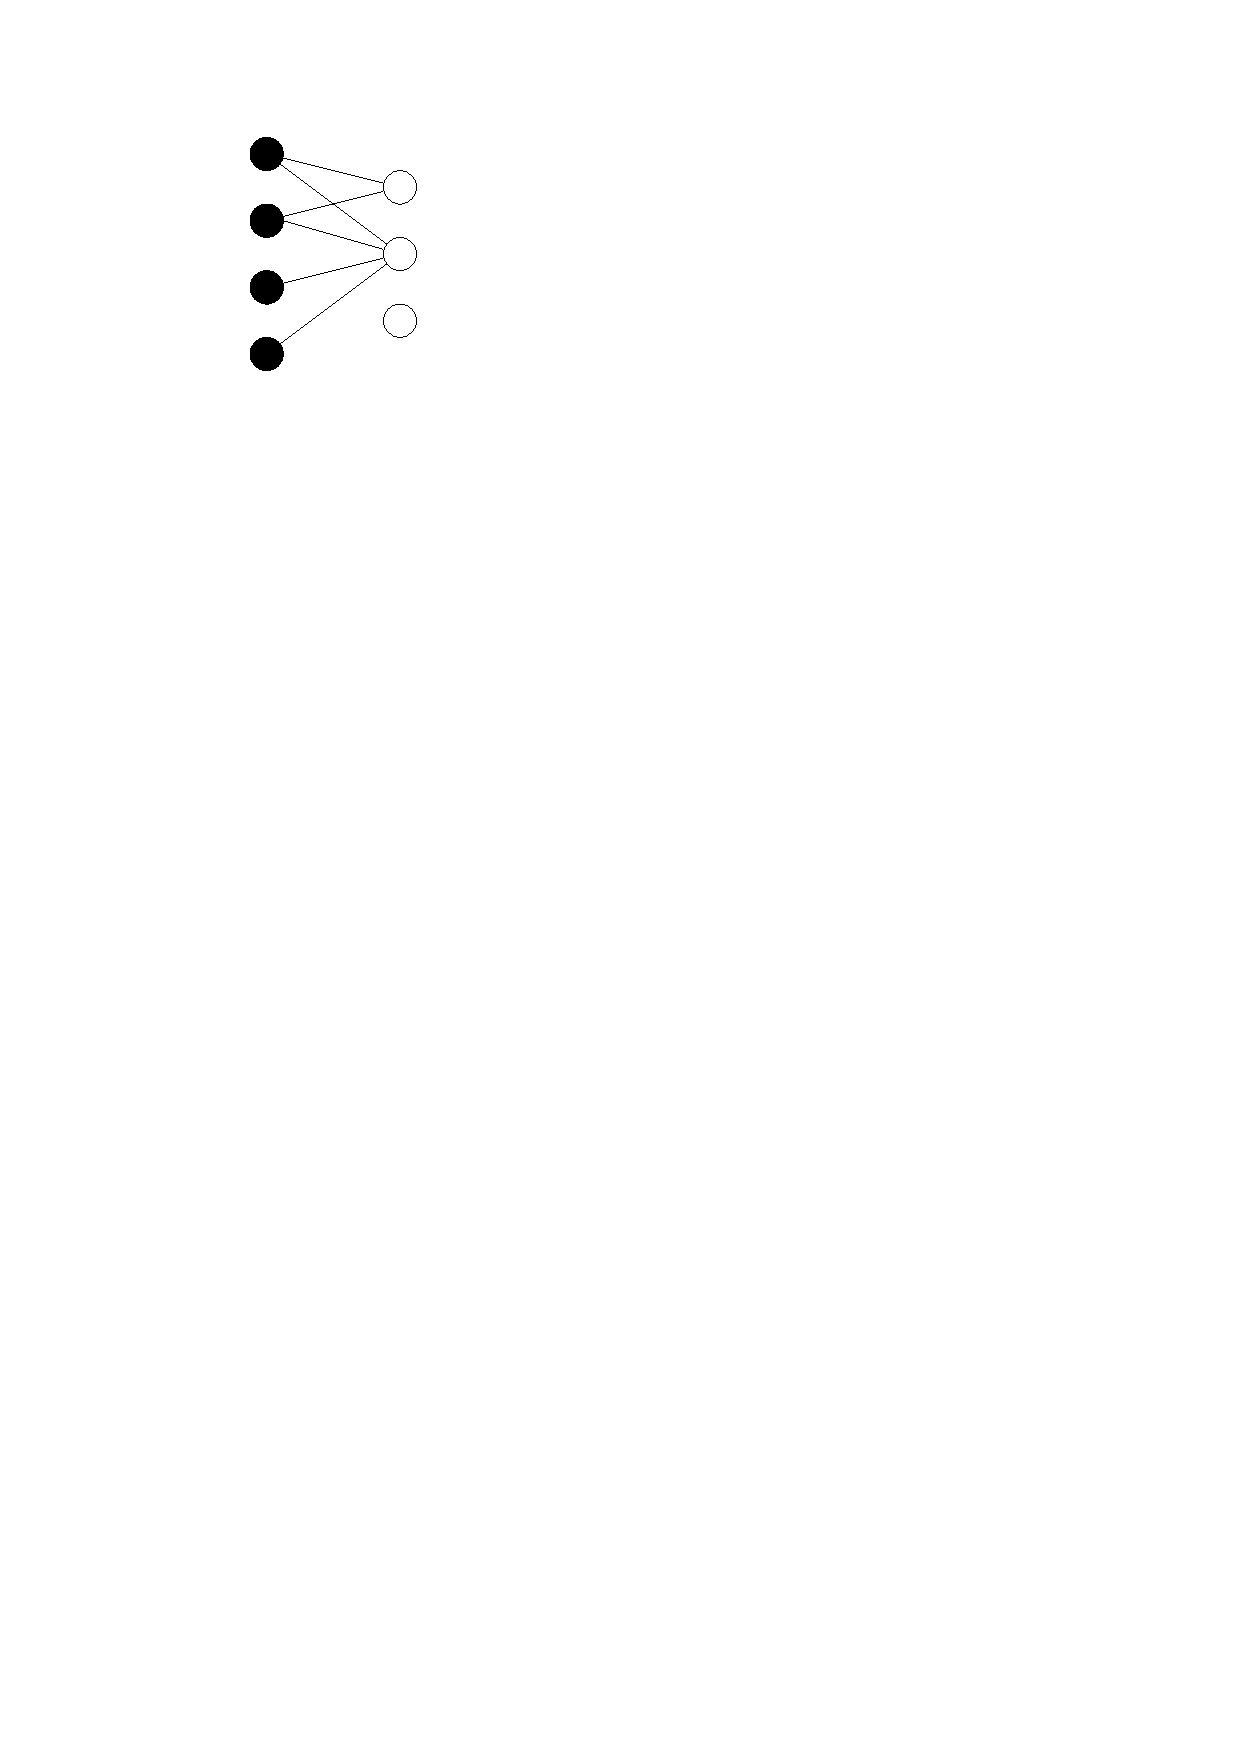
\includegraphics{bipartiteEx} 
\end{center}
\end{Boxample}

There are exponentially many partitions of $V$ into two subsets so we
do not want to have to test all possibilities to determine whether $V$ is bipartite.

\begin{Definition}
Let $k$ be a positive integer. A graph $G$ has a \defnfont{$k$-colouring}
if $V(G)$ can be partitioned into $k$ nonempty disjoint subsets such
that each edge of $G$ joins two vertices in different subsets.
\end{Definition}

\begin{Example}
The graph in \cref{ex:bipartite} has a 2-colouring as indicated.
\end{Example}

It is not just a coincidence that our example of a bipartite graph
has a 2-colouring.

\begin{Theorem} 
The following conditions on a graph $G$ are equivalent.
\begin{itemize}
  \item $G$ is bipartite.
  \item $G$ has a $2$-colouring.
  \item $G$ does not contain an odd length cycle.
\end{itemize}
\end{Theorem}
\begin{proof} 
Given a bipartition, use the same subsets to get a $2$-colouring, and
vice versa. This shows the equivalence of the first two conditions. Now
suppose $G$ is bipartite.  A cycle must have even length, since the start
and end vertices must have the same colour. Finally suppose that $G$
has no odd length cycle. A $2$-colouring is obtained as follows. Perform
BFS and assign each vertex at level $i$ the ``colour" $i \bmod 2$. If we
can complete this procedure, then by definition each vertex goes from
a vertex of one colour to one of another colour. The only problem could
be if we tried to assign a colour to a node $v$ that was adjacent to a
node $w$ of the same colour at the same level $k$. But then a cycle of
length $2k+1$ is created.
\end{proof}

It is now easy to see that we may use the method in the proof above
to detect an odd length cycle if it exists, and otherwise produce a
$2$-colouring of $G$. This of course runs in linear time.


%\section{Maximum matchings}
%\label{sec:matching}
%
%Next we want to introduce an important graph problem that can
%be solved in polynomial time by a clever path augmentation algorithm.  
%
%\begin{Definition}
%A \defnfont{matching} in a graph is a set of pairwise non-adjacent edges
%(that is, each vertex can be in at most one edge of the matching).
%A \defnfont{maximal matching} is a matching such that is not a proper subset
%of any other matching.
%A \defnfont{maximum matching} is one with the largest possible number of
%edges (over all possible matchings).
%\end{Definition}
%
%Often, for many real-world problems, we want to find a maximum matching 
%in bipartite graphs as illustrated by the next two examples.  
%
%\begin{Example}
%Suppose we have a set of workers $V_0$ and a set of tasks $V_1$ that need to be
%assigned.  A given worker of $V_0$ is able to perform a subset of the tasks in $V_1$.
%Now with each worker capable of doing at most one task at a time, the boss 
%would like to assign (match) as many workers as possible to as many of 
%the tasks. 
%\end{Example}
%
%\begin{Example}\label{ex:mp}
%Consider mating fussy kakapo who all live in differnt zoos.  We have a set of males  and females (as vertices) and edges 
%representing compatible mates.  The goal is to mate as many kakapo
%as possible in the current season, which is the same as finding a maximum matching in the
%relationship graph. This is traditionally called the \defnfont{marriage problem}
%\end{Example}
%
%In \cref{fig:matchbipartite} we illustrate the difference between
%a maximal and maximum matching in the setting of \cref{ex:mp}.
%The matchings consist of bold-dashed edges (between females on the left
%and males on the right) in the drawings.
%
%\begin{figure}
%\centering
%\includegraphics{bipartiteMatching}
%\caption{A maximal and maximum matching in a bipartite graph.}
%\label{fig:matchbipartite}
%\end{figure}
%
%It is easy to find a maximal matching $M$ in a graph. For example, 
%a simple greedy approach of
%iterating over all edges and adding each edge to $M$ if it is
%non-adjacent to anything already in $M$ will work.  As illustrated in
%\cref{fig:matchbipartite}, a maximal matching may have fewer
%edges than a more desirable maximum matching.
%
%Our algorithm to compute a maximum matching will be based on
%trying to improve an existing matching $M$ by finding certain
%types of paths in a graph.
%
%\begin{Definition}
%Given a matching $M$, an \defnfont{alternating path} is a path in which 
%the edges 
%of the path alternate from being in the matching and not.
%An \defnfont{augmenting path} is an alternating path that starts from and ends 
%on unmatched vertices.
%\end{Definition}
%
%For example, consider the augmenting path Eve--Doug--Cher--Fred of
%\cref{fig:matchbipartite}.  It contains three edges but only the
%middle edge is part of a matching on the left case.  We can get the
%better matching on the right if we add Eve-Doug, remove Doug--Cher, and add 
%Cher--Fred to the existing matching.  Thus, in general, we see that we can 
%improve a matching if we can find an augmenting path.  Note that there is always one
%more non-matching edge than matching edge in an augmenting path.
%Likewise, it is pretty easy to show that if there is no such augmenting path 
%then we must have a maximum matching (see Exercise~\ref{ex:agpath}).
%
%We next present a polynomal-time algorithm that finds an augmenting path if
%one exists.  The basic idea is to start from an unmatched vertex $v$
%and build a tree (via a graph traversal algorithm such as BFS) 
%of alternating paths away from $v$.  If we reach another unmatched vertex 
%then we have found an augmenting path.  Otherwise, if we visit all vertices
%(in the same component as $v$) then we conclude that no augmenting 
%path exists starting at $v$.  This algorithm is given in \cref{fig:augpath}.
%
%
%%\begin{algorithm}[H]
%%  \caption{An algorithm to find an augmenting path, given a matching
%%and an unmatched starting vertex.}
%%    \label{alg:augpath}
%%\begin{algorithmic}[1]
%%\Function{findAugmentingPath}{bipartite graph $G$; matching $M$; unmatched vertex $x$}
%%	\State queue $Q$
%%	\State array $\status[0..n-1]$, $\pred[0..n-1]$
%%	\For{$u \in V(G)$}
%%  		\State $\status[u] \gets $ WHITE; $\pred[u] \gets $ \texttt{null} 
%%	\EndFor
%%	\State $\status[x] \gets $ EVEN
%%	\State $Q$.\algfont{insert}$(x)$
%%	\While{\textbf{not}  $Q$.\algfont{isEmpty}$()$}
%%		\State $u \gets Q$.\algfont{pop}$()$
%% 		\If{$\status[u] =$ EVEN}
%% 			\For{each $v$ adjacent to $u$}
%% 				\If{$\status[v]$ = WHITE}
%% 					\State $\status[v] \gets$ ODD; $\pred[v] \gets$ u
%% 					\If{$v$ is unmatched in $M$}
%% 						\State \Return{path $x,\ldots, \pred[\pred[u]], \pred[u], u, v$}
%% 					\Else
%%	 					\State $Q$.\algfont{insert}$(v)$
%% 					\EndIf
%% 				\EndIf
%% 			\EndFor
%% 		\Else 			\Comment{that is, $\status[u] =$ ODD} 
%%			\State $v \gets$ matched vertex of $u$ from $M$
%%			\If{$status[v]$ = WHITE}
%%				\State$\status[v] \gets$ EVEN; $\pred[v] \gets u$
%% 				\State$Q$.insert$(v)$
%%	 		\EndIf
%% 		\EndIf
%%	\EndWhile
%%	\State \Return{false} \Comment{no augmenting paths containing $x$}
%%\EndFunction
%%\end{algorithmic}
%%\end{algorithm}
%
%
%
%\begin{Theorem}
%There exists a polynomial-time algorithm to find a maximum matching
%in a bipartite graph.
%\end{Theorem}
%%\begin{proof}
%%We first need to show that the algorithm \algfont{findAugmentingPath}, given in
%%\cref{fig:augpath}, does find an augmenting path if one exists.
%%It is sufficient to show that if there exists at least one augmenting path 
%%from vertex $x$ to some other unmatched vertex that we find any one of them 
%%(in our case, by imitating BFS, it will be one of shortest length).  
%%\algfont{findAugmentingPath}
%%builds a traversal tree starting at $x$ using the following constraints.
%%\begin{itemize}
%%\item If a reachable vertex $u$ is in the same partition as $x$ (status will
%%be set to EVEN by the algorithm) then we know (except for $x$) that there is 
%%an alternating path with the last edge including $u$ being in the matching.
%%\item If a reachable vertex $v$ is not in the same partition as $x$ (status will
%%be set to ODD if it is matched) then we know that there is 
%%an alternating path with the last edge including $v$ is not in the matching.
%%\end{itemize}
%%This process produces a tree with alternating paths rooted at $x$ as 
%%illustrated in \cref{fig:augtree}.  The status of the nodes are ODD 
%%or EVEN depending if they are an even or odd distance from $x$.  If a vertex 
%%(first seen) is at an odd distance then we have seen an alternating path 
%%where the last edge is not in the matching.  If this last vertex is unmatched 
%%then we have found an augmenting path, otherwise we extend the path by using 
%%the matched edge.  
%%If a vertex is at an even distance then we have seen an alternating path
%%where the last edge is in the matching.  Since the graph is bipartite the
%%status of being ODD or EVEN is unambiguous.
%%
%%\begin{figure}
%%\centering
%%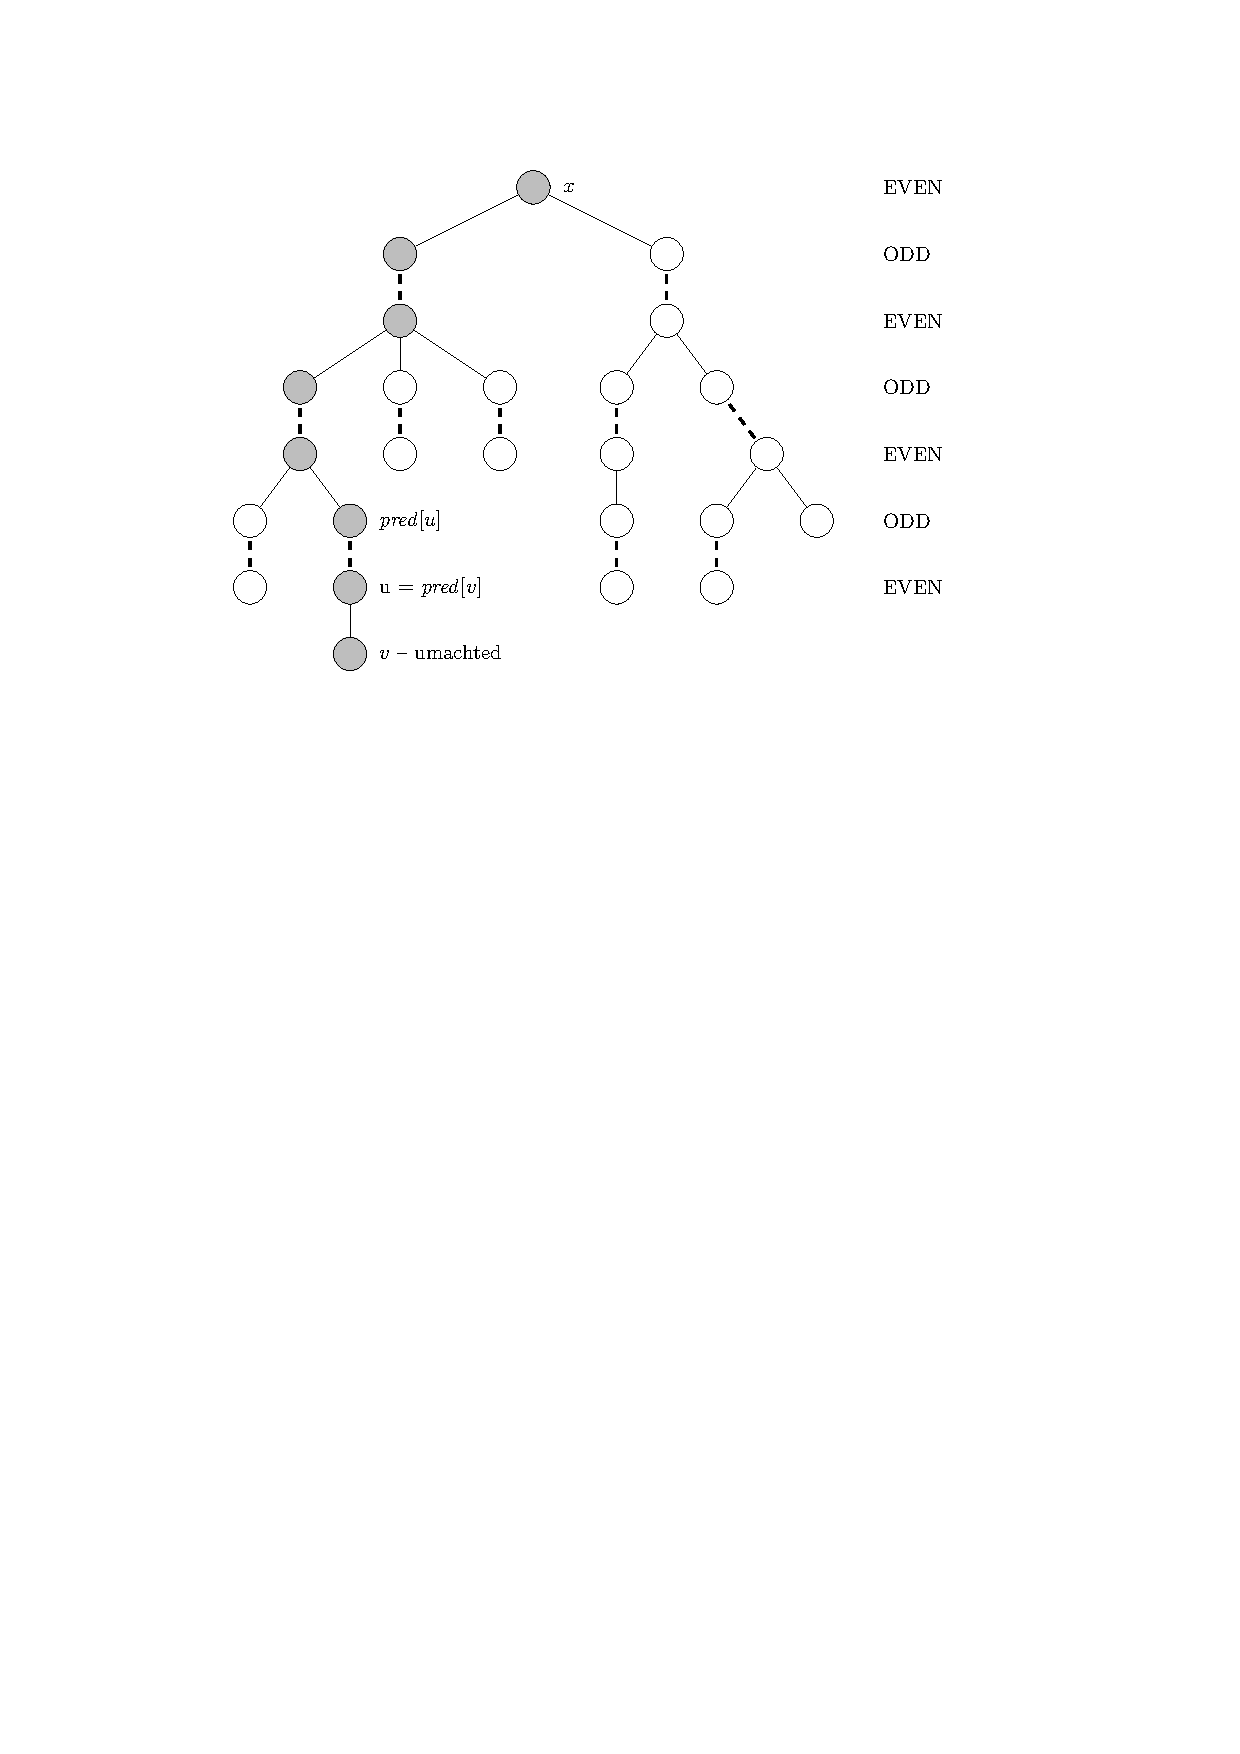
\includegraphics{augtree} 
%%\caption{Structure of the graph traversal tree for finding augmenting paths.}
%%\label{fig:augtree}
%%\end{figure}
%%
%%Suppose the algorithm \algfont{findAugmentingPath} terminates without
%%finding an augmenting path when one does exist.  Let $x=v_0,v_1,\ldots,v_k$
%%be a counterexample.  Consider the
%%first index $0<i\leq k$ such that $status[v_i] =$ WHITE.  We know $v_{i-1}$ was
%%inserted in the queue $Q$. Consider the two cases.  If $i-1$ is even then
%%since $v_i$ is a neighbour of $v_{i-1}$ its status would have changed to
%%ODD.
%%If $i-1$ is odd then either $(v_{i-1},v_i)$ is in the matching or not.
%%If so, the status of $v_i$ would have changed; if not, a prefix of the 
%%counterexample is not an augmenting path.  Thus, by contradiction,
%%\algfont{findAugmentingPath} will find an augmenting path if one exists.
%%
%%The running time of one invocation of \algfont{findAugmentingPath} is the same 
%%as the running time of BFS since each vertex is added to the queue $Q$
%%at most once.  For adjacency list representation of graphs this 
%%can be carried out in time $O(m)$.  If we find an augmenting path
%%then our best matching increases by one.  
%%Since a maximum matching is bounded by $\lfloor n/2 \rfloor$ we
%%only need to find at most $O(n)$ augmenting paths.
%%We potentially need to call \algfont{findAugmentingPath}
%%once for each unmatched vertex, which is bounded by $O(n)$, and 
%%repeat the process for each modified matching.  Therefore, the total 
%%running time to find a maximum matching is at most $O(n^2m)$.
%%\end{proof}
%
%The algorithm presented here can easily be improved to $O(nm)$ by
%noting that it is only required to traverse and compute an 
%``alternating path forest'' in order to find an augmenting path.  
%That is, we do not need to originate a call to \algfont{findAugmentingPath} for all 
%unmatched vertices. However the correctness is a bit tricky to justify.
%
%There are other algorithms that find maximum matchings more efficiently
%than the one presented.  One of these is the Hopcroft-Karp algorithm
%which runs in time $O(m\sqrt{n})$ and is based on finding a maximal 
%flow in a network (by adding a source and sink vertex and directing all edges
%from one vertex partition to the other of the bipartite graph).
%
%We conclude this section by mentioning that there also exist
%poly\-nomial-time algorithms to find maximum matchings in arbitrary
%(non-bipartite) graphs. The details are beyond the scope of this book.
%
%%\subsection*{Exercises}
%
%\begin{Exercise}\label{ex:agpath}
%Prove that a matching for a graph is maximum if and only if it does not
%have any augmenting paths.
%\end{Exercise}
%
%\begin{Exercise}
%Give an example of a bipartite graph of order 12 with a maximal matching 
%that has an augmenting path of length 5 and a maximum matching of 
%the same graph with two more edges.
%\end{Exercise}
%
%%\if 01
%%\begin{Exercise}
%%Explain what changes need to be done to the algorithm
%% \algfont{findAugmentingPath} 
%%so that it runs in time $O(|E|)$ and traverses all of the bipartite graph
%%(instead of just the tree reachable from the unmatched vertex $x$).
%%\end{Exercise}
%%\fi
%
%\begin{Exercise}\label{ex:konig}
%Show that the size of a maximum matching in a bipartite graph $G=(V,E)$ is the
%same as the size of the smallest \defnfont{vertex cover} of $G$.  A vertex cover
%is a subset $V' \subseteq V$ of vertices such that for 
%all $(u,v) \in E$, at least one of $u$ or $v$ is in $V'$.
%Does the equality hold for arbitrary graphs?
%\end{Exercise}
%
%\section{Notes}
%
%The linear-time algorithm for finding strong components of a digraph was 
%introduced by R. E. Tarjan in 1971.
%
%One of the early polynomial-time algorithms for finding
%maximum matchings in bipartite graphs is based on the Ford--Fulkerson 
%network flow algorithm \cite{FF56} from 1956.
%The first polynomial-time algorithm for finding a maximum matching in an 
%arbitrary graph was presented by J.~Edmonds \cite{Ed65} in 1965.

%[FF56]
%L. R. Ford and D. R. Fulkerson 
%"Maximal flow through a network". 
%\textit{Canadian Journal of Mathematics} \textbf{8} (1956), pp 399--404.

%[Ed65]
%J. Edmonds.  Paths, trees, and flowers
%\textit{Canadian Journal of Mathematics} \textbf{17} (1965), pp. 449-467. 

\part{Weighted digraphs and optimization problems}
\label{ch:weighted}

\chapter{Weighted graphs, the single-source shortest paths problem, Dijkstra} %----------
Weighted digraphs encode not only information about \boldfont{whether} one can get from $A$ to $B$,
but \boldfont{how much it will cost} to do so.
The weight could represent the cost of using a link in a communication network, 
or distance between nodes in a transportation network. 
We use the terms of cost and distance interchangeably.

% We need a different ADT for this purpose. 

\section{Weighted digraphs} \label{sec:weighted}
\begin{Definition}
A \defnfont{weighted digraph} is a pair $(G, c)$ where $G$ is a digraph
and $c$ is a \defnfont{cost function} associating a real number to each arc of $G$. 
For an arc $(u,v)$, we interpret  $c(u, v)$ as the \defnfont{cost} of using $(u, v)$.
\end{Definition}

An ordinary digraph can be thought of as a special type of weighted digraph 
where the cost of each arc is $1$. 
%A weighted graph may be represented as a symmetric digraph where 
%each of a pair of antiparallel arcs has the same weight.

\begin{Boxample} \label{ex:graphExWeighted}
A classic unweighted graph (called the $3$-cube), a digraph with arc weights, 
and a graph with edge weights.
\begin{center}
 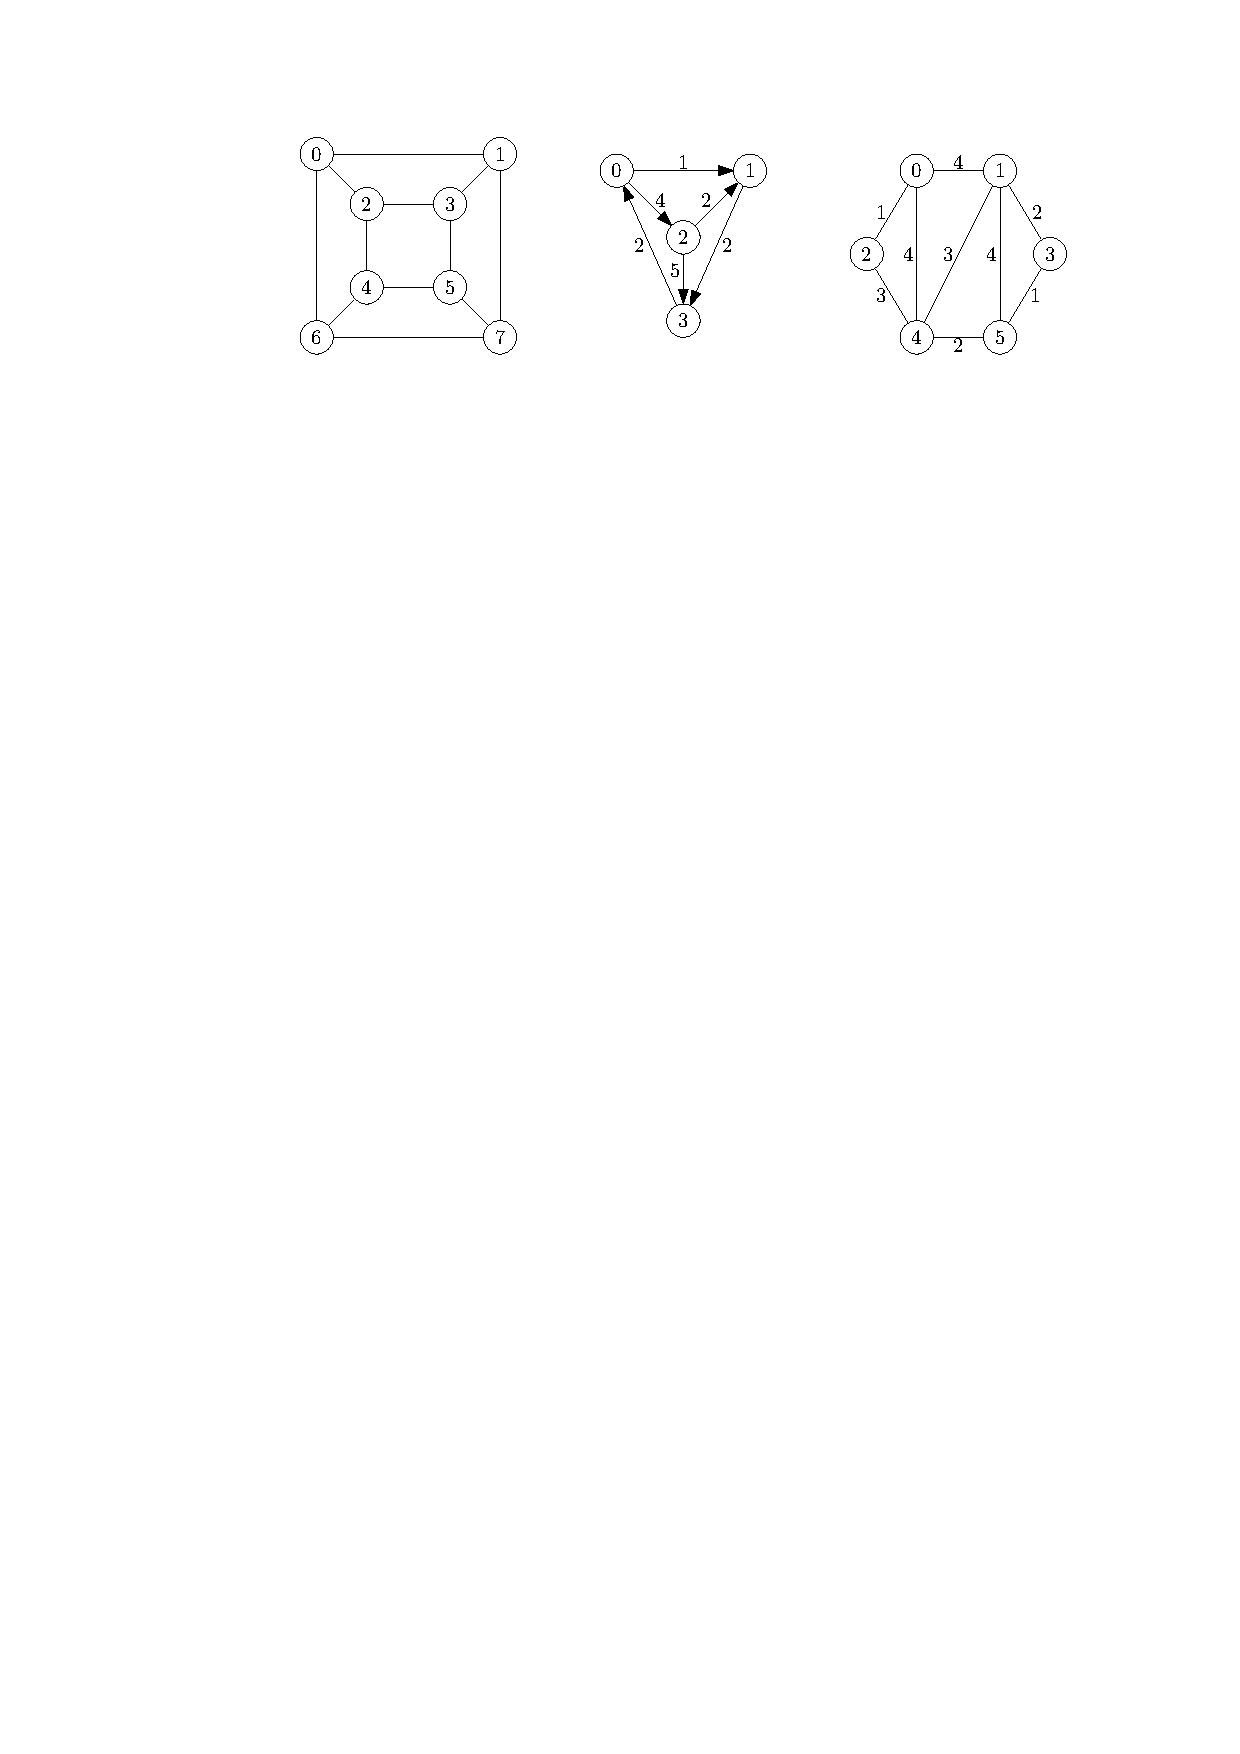
\includegraphics{graphExWeighted}
\end{center}
\end{Boxample}

Weighted digraphs can be represented using adjacency matrices or lists:
\begin{itemize}
  \item The adjacency matrix is modified so that each entry of $1$ (signifying that an arc exists) 
  is replaced by the cost of that arc.
  \item Care needs to be taken if using 0 to represent the absence of arcs, as 0 may be a legal edge weight. 
  In these cases, \texttt{null}, $\infty$ or some suitable value may be used.
  We use \boldfont{the convention that 0 or} \texttt{null} \textbf{represents the absence of an arc}. 
  \item An adjacency list is modified so that the list associated  with node $v$ has each adjacency node followed by the cost of the arc to the adjacent node. 
  \item For example, the list for node 6 with adjacent arcs $(6,2)$ with $c(6,2) = 4$ and $(6,7)$ with $c(6,7) = 5$ would be $2,4,7,5$.
\end{itemize}

\begin{Boxample}[0] \label{ex:drawWeightedGraph}
Draw the weighted graph given by the weighted matrix below. 
\newline

$\left[
\begin{array}{cccc}
	0 & 3 & 4 & 0  \\
	3 & 0 & 1 & 3  \\
	4 & 1 & 0 & 2  \\
	0 & 3 & 2 & 0  \\
\end{array}
\right]$
\vspace{1cm}


Draw the weighted digraph given by the weighted list representation below.
\newline

$\AdjLists{
\begin{tabular}{c|llll}
	0 & 1 & 3 & 2 & 4 \\
	1 & 0 & 2 & 3 & 2 \\
	2 & 1 & 3 &   &   \\
	3 & 2 & 1 &   &   \\
\end{tabular}
}$
\end{Boxample}


\section{Distance and diameter} \label{sec:unweighted}
Recall that the distance $d(u,v)$ between nodes $u$ and $v$ in an (unweighted) digraph 
is simply the number of arcs in the shortest path between them. 

In a weighted digraph, the distance to from node $u$ to $v$,  $d(u,v)$, is the cost of the minimum cost path from $u$ to $v$ where the cost of a path is just the sum of the costs on that path.


\begin{itemize}
  \item It is often helpful to have the \defnfont{distance matrix} for a digraph.
  The $(i, j)$-entry of this matrix contains the distance between node $i$ and node $j$.
  \item For an unweighted digraph, the distance matrix can be generated by running \texttt{BFSvisit}
  from each node in turn, since the distance to a node is equal to its depth in the BFS tree 
  (or infinite if the node is not reachable from the start node so not in the tree). 
  This gives an algorithm with running time in $\Theta(n^2 + nm)$.
\end{itemize}

\begin{Boxample}
A graph, its adjacency matrix and its distance matrix.\\

\begin{minipage}[c]{0.3\textwidth}
\centering
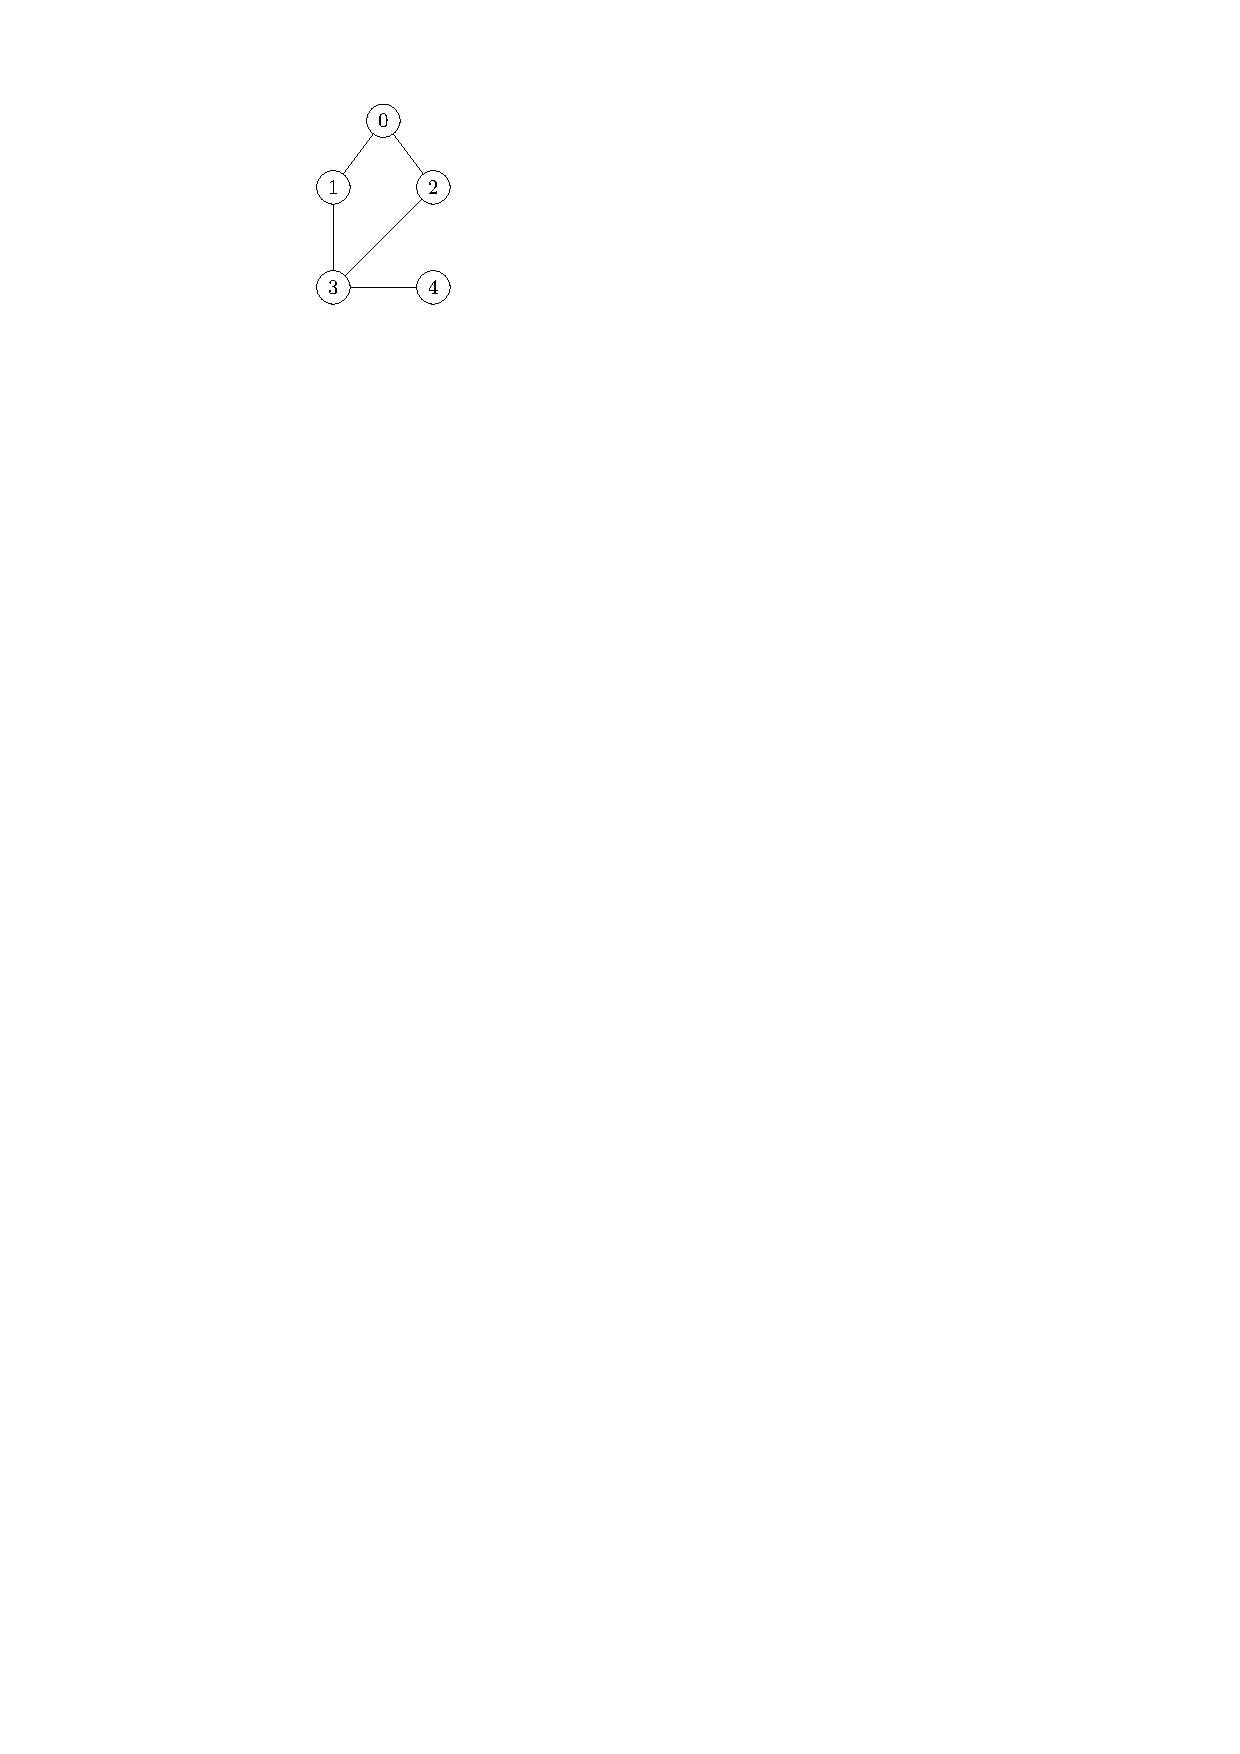
\includegraphics{distanceMatrixGraph}
\end{minipage}
\begin{minipage}[c]{0.65\textwidth}
$$\quad\left[
\begin{array}{ccccc}
0 & 1 & 1 & 0 & 0 \\
1 & 0 & 0 & 1 & 0 \\
1 & 0 & 0 & 1 & 0 \\
0 & 1 & 1 & 0 & 1 \\
0 & 0 & 0 & 1 & 0 \\
\end{array}
\right]
\hspace{1.5cm}
\left[
\begin{array}{ccccc}
0 & 1 & 1 & 2 & 3 \\
1 & 0 & 2 & 1 & 2 \\
1 & 2 & 0 & 1 & 2 \\
2 & 1 & 1 & 0 & 1 \\
3 & 2 & 2 & 1 & 0 \\
\end{array}
\right]$$
\end{minipage} 
\end{Boxample}

\begin{Boxample}[6]
Give an example of a weighted digraph in which the BFS approach
does not find the shortest path from the root to a node.
\end{Boxample}

\begin{Definition} \label{def:diameter}
The \defnfont{diameter} of a strongly connected digraph $G$ is the
maximum of $d(u,v)$ over all nodes $u, v \in V(G)$. 
If the digraph is not strongly connected the diameter is undefined though can be set to $\infty$.

\end{Definition}

 Clearly the diameter is just the maximum entry in the distance matrix.

\begin{Boxample}[1]
What is the diameter of the 3-cube in \cref{ex:graphExWeighted}?

\end{Boxample}

\section{Single-source shortest path problem} \label{sec:SSSP}
\begin{Definition}
In  the \defnfont{single-source shortest path problem} (SSSP) 
we are given a weighted digraph $(G, c)$ and a source node $s$. 
For each node $v$ of $G$, we must find the minimum weight of a path from $s$ to $v$.
By the weight of a path we mean the sum of the weights on the arcs. 
This is like finding row $s$ in a weighted distance matrix.
\end{Definition}

\begin{Boxample} \label{eg:SSSP}
In the weighted digraph pictured, the unique shortest path from $0$ to $3$ is $0, 1, 3$ with weight $3$.
What is the path with minimum weight from $2$ to $0$, and what is its weight?\\

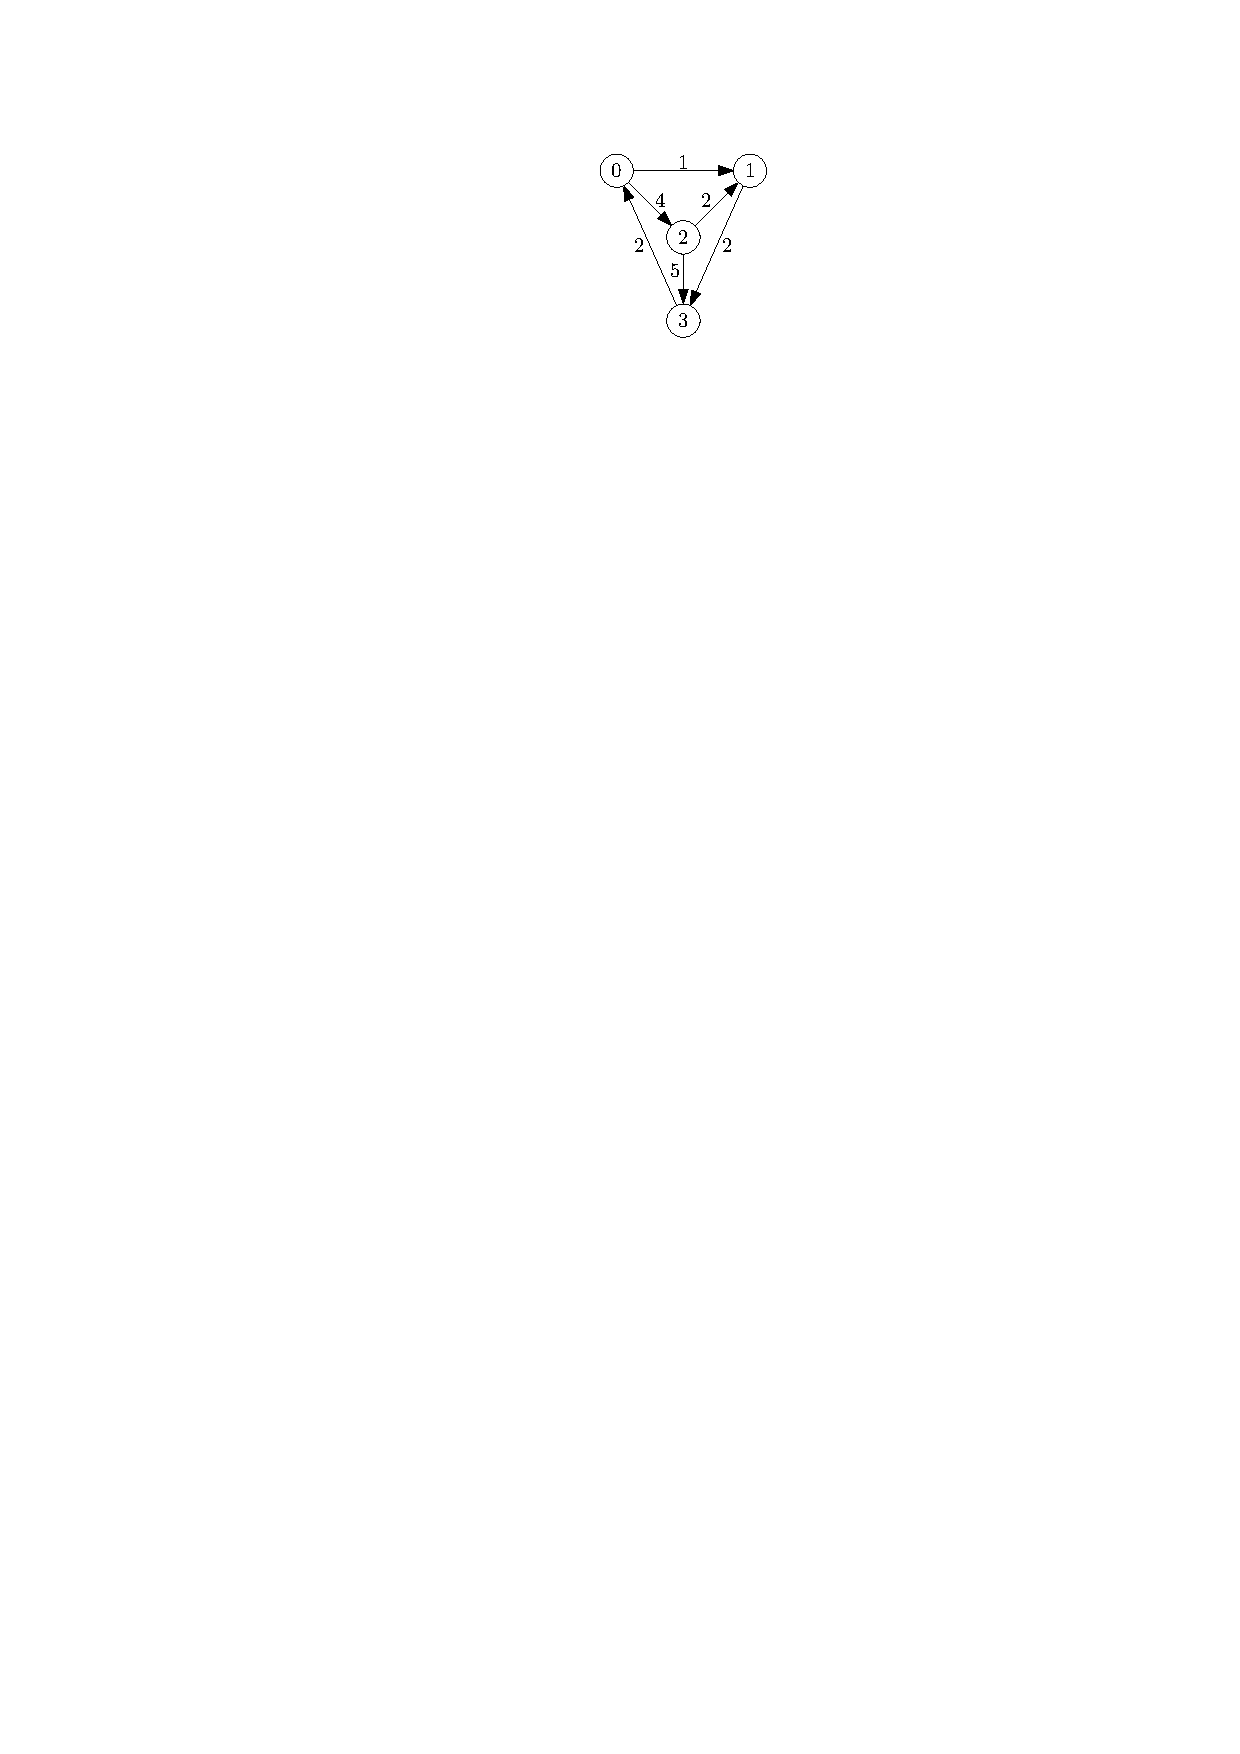
\includegraphics{weightedDigraph}
\end{Boxample}

\section{Dijkstra's algorithm}
\defnfont{Dijkstra's algorithm} solves the SSSP problem whenever \boldfont{all weights are non-\linebreak[4]negative}. 
It may fail in the presence of negative weight arcs.

It is easiest to understand the algorithm in terms of a set of visited nodes $S$, which eventually includes all nodes in $G$. 
We'll consider only shortest paths through $S$. % and make sure the length of these shortest paths is accurate.
Once $S = V(G)$, all shortest path lengths are known. 

Initially $S$ contains only the single node $s$. 
The only paths available are the one-arc paths from $s$ to neighbours $v$, of weight $c(s, v)$. 
We choose the neighbour $u$ with $c(s, u)$ minimal and add it to $S$. 

Now the fringe nodes adjacent to $s$ and $u$ must be updated to reflect possible paths through $u$ 
(it is possible that there exists a path from $s$ to $v$, passing through $u$, that is shorter than the direct path from $s$). 
Now we choose the node whose current best distance to $s$ is smallest, and update again. 
We continue in this way until all nodes belong to $S$. In \cref{alg:dijkstra}, the set $S$ consists of the BLACK nodes.

\begin{algorithm}[H]
  \caption{Dijkstra's algorithm, first version.}
    \label{alg:dijkstra}
\begin{algorithmic}[1]
\Function{Dijkstra}{weighted digraph $(G, c)$; node $s \in V(G)$}
	\State array $\colour[0..n-1]$, $\dist[0..n-1]$
	\For{$u \in V(G)$}
		\State $\dist[u] \gets c[s,u]$; $\colour[u] \gets$ WHITE 
	\EndFor
	\State $\dist[s] \gets 0$; $\colour[s] \gets $ BLACK
	\While{there is a white node}
		\State find a white node $u$ so that $\dist[u]$ is minimum
		\State $\colour[u] \gets $ BLACK
		\For{$x \in V(G)$}
			\If{$\colour[x] = $ WHITE}
				\State $\dist[x] \gets \min \{\dist[x], \dist[u] + c[u,x]\}$  
			\EndIf
		\EndFor
	\EndWhile
	\State \Return{$\dist$}
\EndFunction
\end{algorithmic}
\end{algorithm}

\begin{Boxample}
An application of Dijkstra's algorithm with starting vertex $0$. 
The distances to 0 at each step are displayed next to each node.
\begin{center}
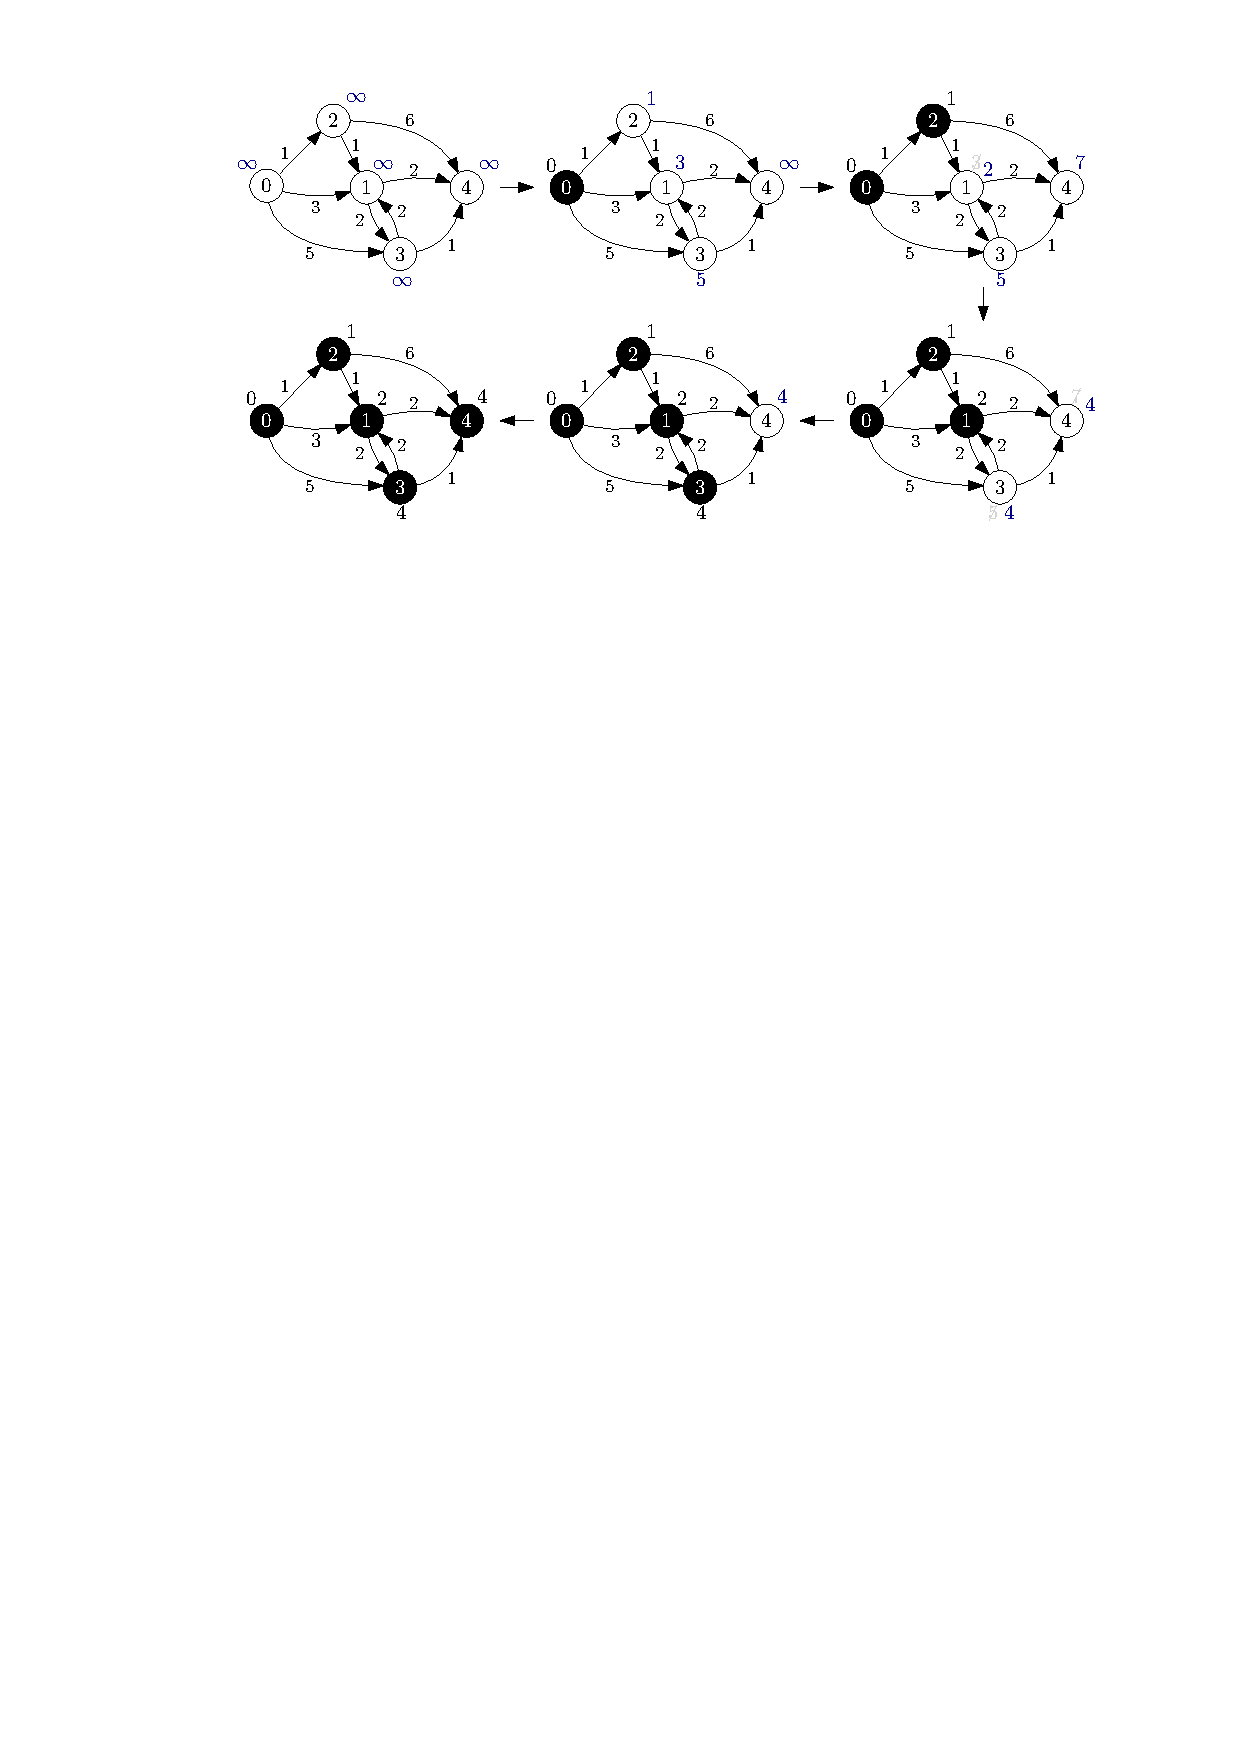
\includegraphics[width=1.0\textwidth]{DijkstraEx2}
\end{center}
\end{Boxample}

Dijkstra's algorithm is an example of a \defnfont{greedy algorithm}. 
At each step it makes the best choice involving only local information,
and never regrets its past choices. 

\begin{Boxample}\mbox{}\\
  \label{ex:dijs-all-vert}
  \begin{minipage}[c]{0.45\textwidth}
	An application of Dijkstra's algorithm on the digraph below
	for each starting vertex $s$. 
	Complete the table for the starting vertex 2.
	
	\begin{center}
	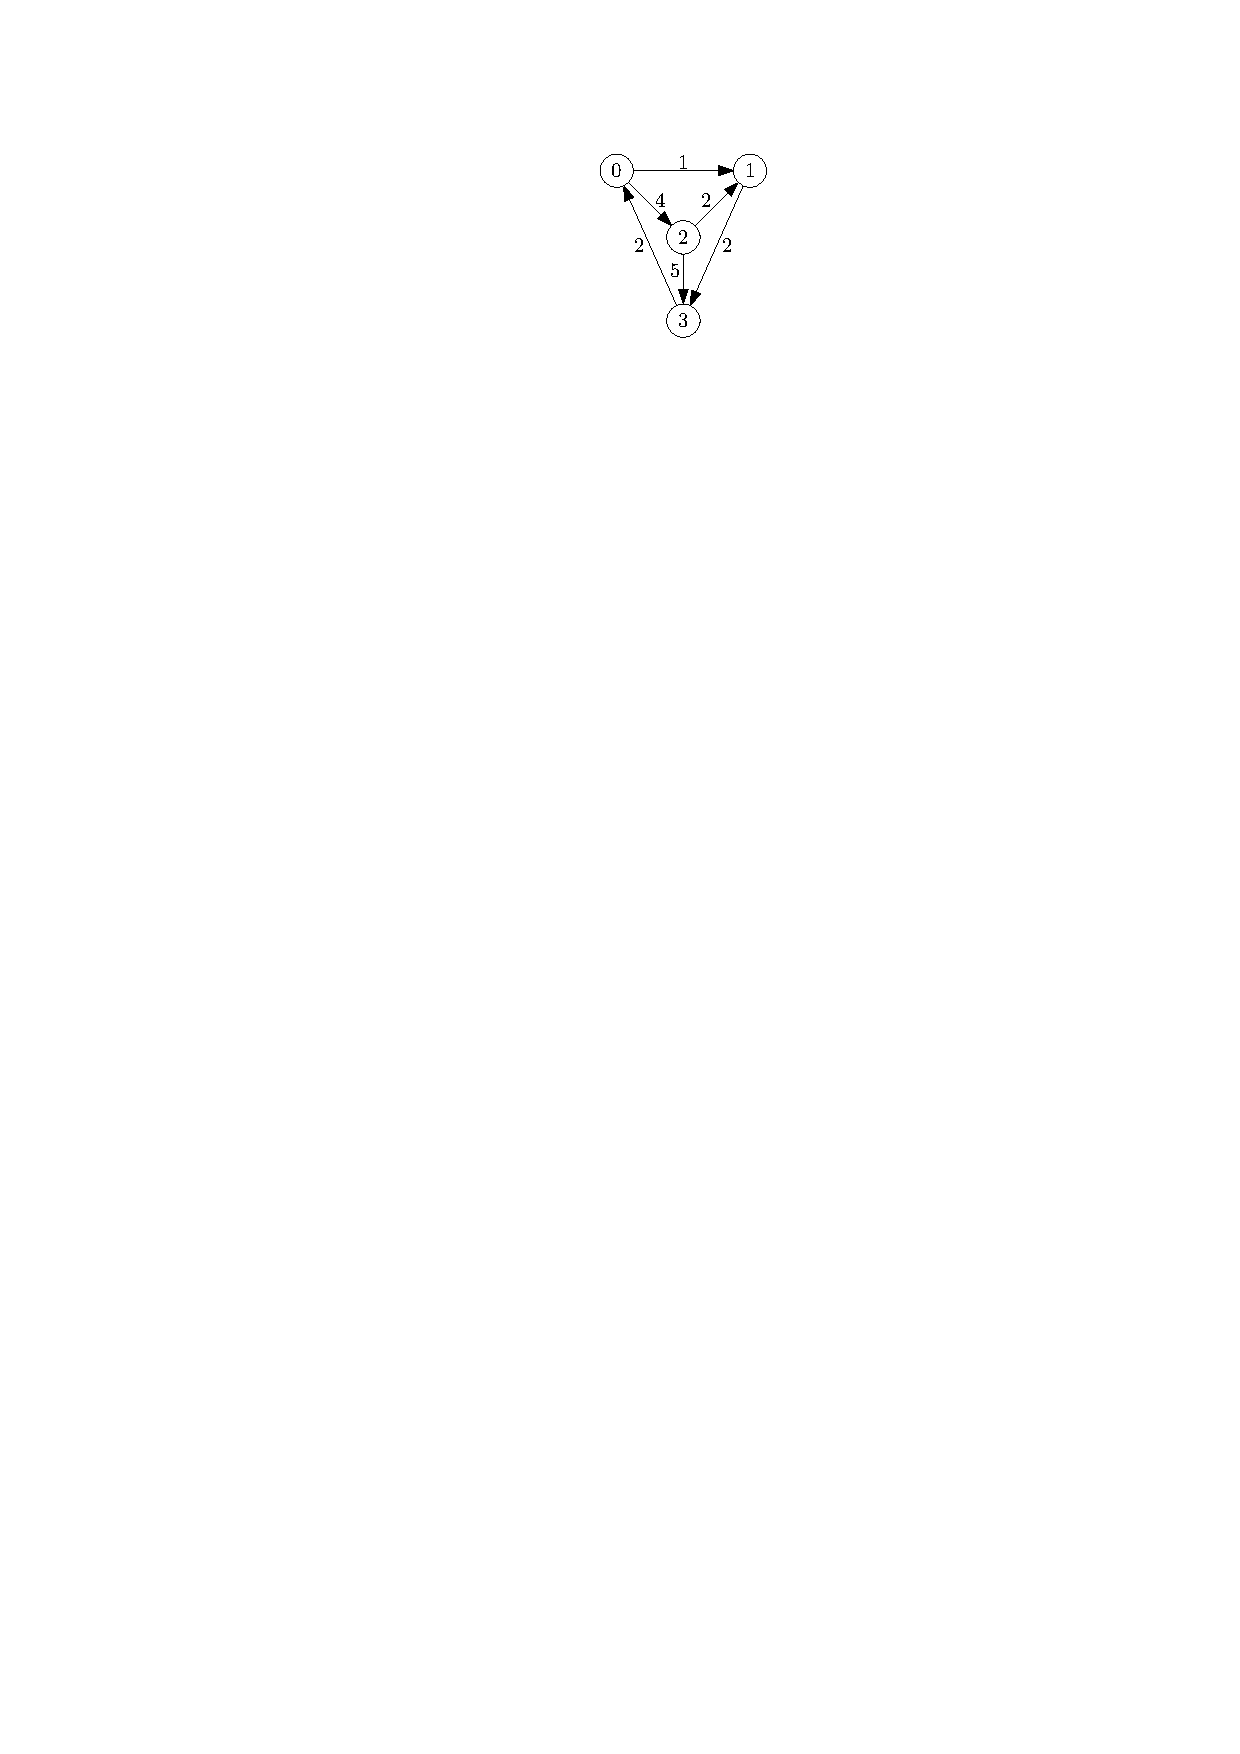
\includegraphics{weightedDigraph}
	\end{center}
	
	The table illustrates that the distance vector is updated at 
	most $n - 1$ times (only before a new vertex is selected and added to $S$). 
	Thus we could have omitted the lines with $S = \set{0,1,2,3}$.
  \end{minipage}$\quad$
  \begin{minipage}[c]{0.45\textwidth}
	\begin{tabular}{|c|c|}\hline
		\textbf{current} $S \subseteq V$ &  \textbf{distance vector} $\dist$ \\ \hline
		\set{0}       & $0, 1, 4, \infty$  \\
		\set{0,1}     & $0, 1, 4, 3$  \\
		\set{0,1,3}   & $0, 1, 4, 3$  \\
		\set{0,1,2,3} & $0, 1, 4, 3$  \\ 
			\hline
		\set{1}       & $\infty, 0, \infty, 2$  \\
		\set{1,3}     & $4, 0, \infty, 2$ \\
		\set{0,1,3}   & $4, 0, 8, 2$ \\
		\set{0,1,2,3} & $4, 0, 8, 2$ \\ 
		\hline
		\set{2}           & \\%$\infty, 2, 0, 5$  \\
		&\\
		\set{\qquad}      & \\%$\infty, 2 , 0, 4$ \\
		&\\
		\set{\qquad\quad} & \\%$6, 2, 0, 4$  \\
		&\\
		\set{0,1,2,3}     & \\ %\hline %$6, 2, 0, 4$ \\ \hline
		&\\ \hline
		\set{3}       & $2, \infty, \infty, 0$ \\
		\set{0,3}     & $2, 3, 6, 0$ \\
		\set{0,1,3}   & $2, 3, 6, 0 $ \\
		\set{0,1,2,3} & $2, 3, 6, 0$ \\ \hline
	\end{tabular}
  \end{minipage}\\
\end{Boxample}


\chapter{Dijkstra proof and running time} %--------------------------------------
\begin{Boxample}[0.5] \label{ex:dijk-neg-fails}
Give weights to the edges of the digraph below so that running Dijkstra's algorithm 
with starting vertex $0$ fails. 
\vspace{0.5cm} 
\begin{center}
  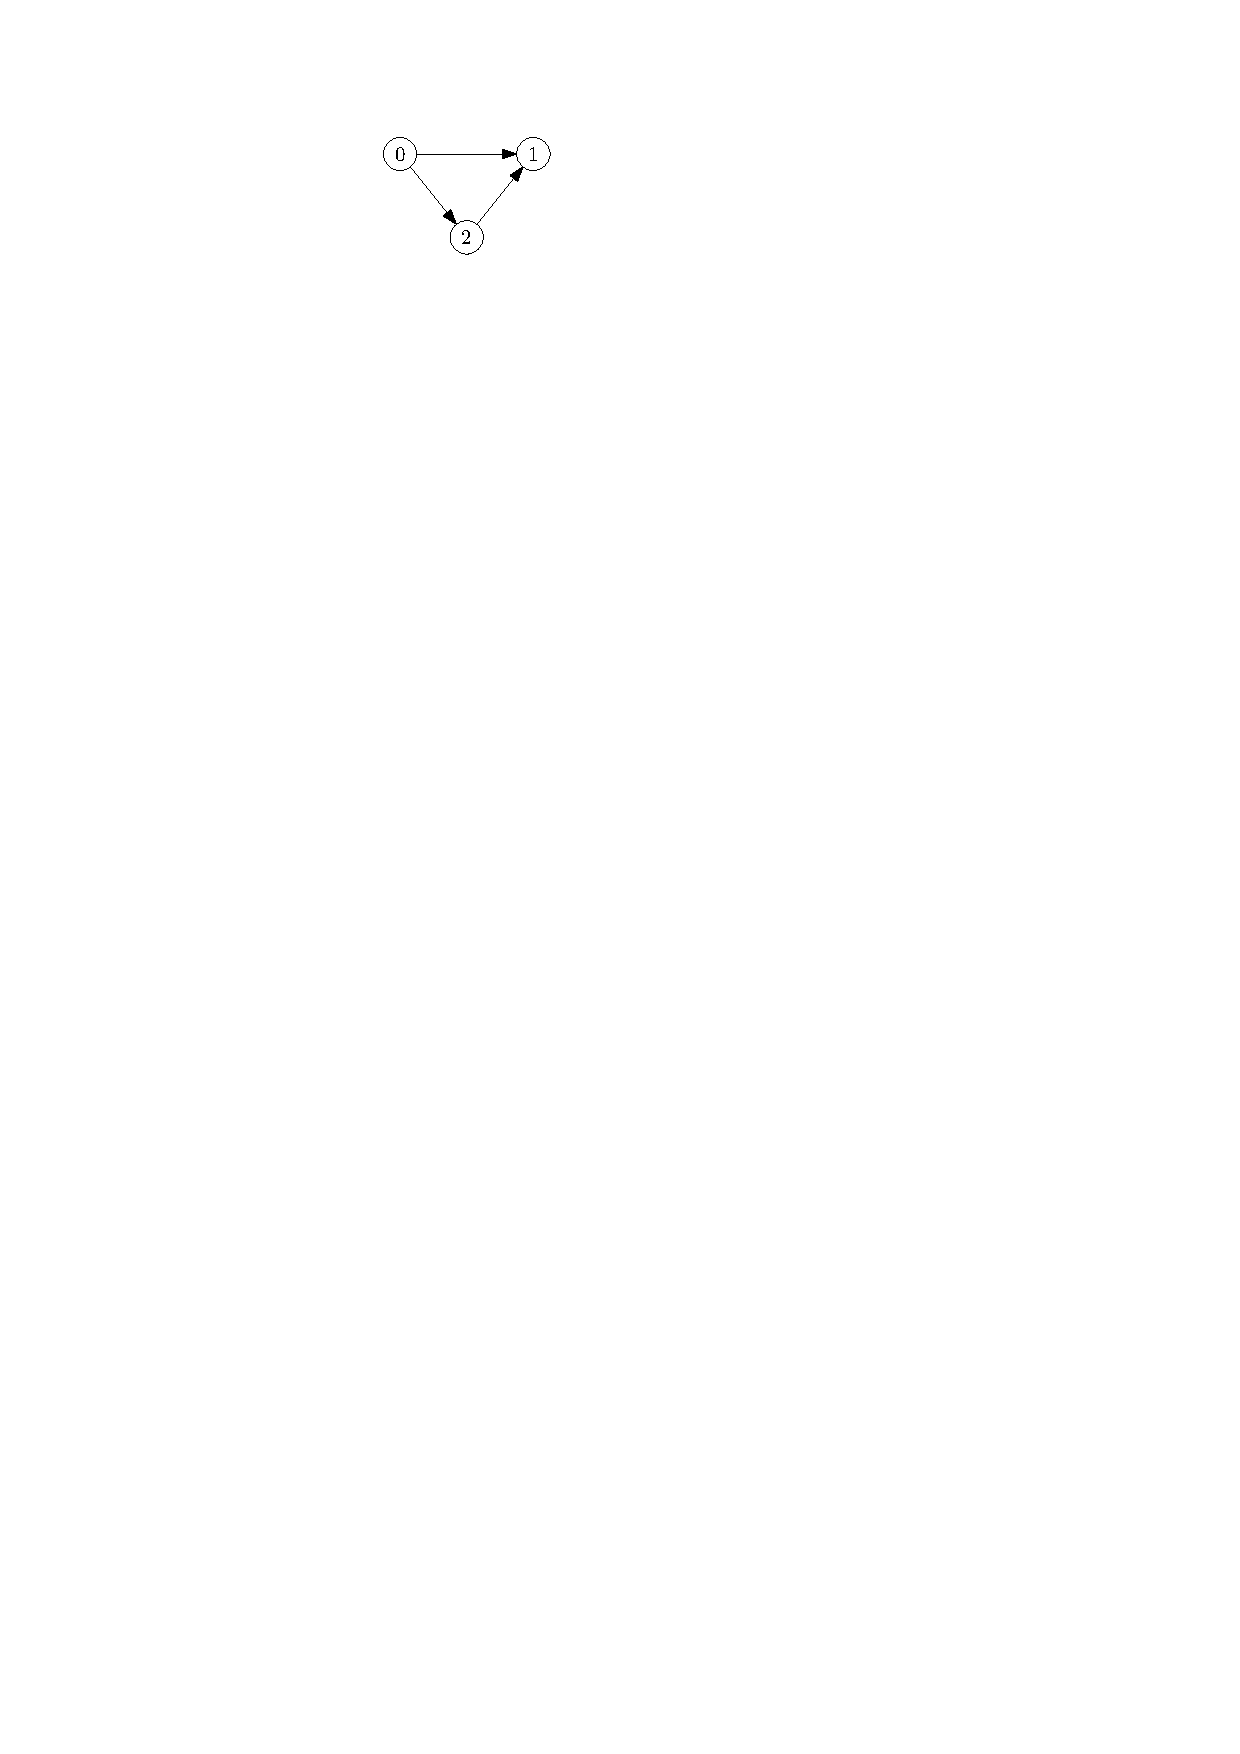
\includegraphics{DijkstraTriangle}
\end{center}
\end{Boxample}

Proving Dijkstra's algorithm works is trickier than for other algorithms we've seen.

Define an \defnfont{$\boldsymbol S$-path} from $s$ to $w$ as a
path from $s$ to $w$ with $s$ and all intermediate nodes belonging to $S$. 
In other words, $w$ may not belong to $S$, but all other nodes in the path do.

\begin{Theorem}
\label{thm:dijkstra} Suppose that all arc weights are non-negative. 
Then at the top of the \boldfont{while} loop, we have the following properties:
\begin{description}
  \item[P1:] If $x \in V(G)$, then $\dist[x]$ is the minimum cost of an $S$-path from $s$ to $x$.
  \item[P2:] If $w \in S$, then $\dist[w]$ is the minimum cost of a path from $s$ to $w$.
\end{description}
\end{Theorem}
%\begin{proof} 
At every step, $\dist[x]$ is the length of some path from $s$ to $x$, or $\infty$. 
That path is an $S$-path if $x \in S$. 
Also note that the update formula ensures that $\dist[x]$ never increases. 

To prove P1 and P2, we use induction on the number of times $k$ we
have been through the while-loop. Let $S_k$ denote the value of $S$
at this stage. 

\begin{Boxample}[3]
Show that P1 and P2 hold when $k = 0$.
\end{Boxample}
\begin{Boxample}[9]
Show that P1 holds for any value of $k$.
\end{Boxample}
\begin{Boxample}[9]
Show that P2 holds for any value of $k$ and that this proves the correctness of Dijkstra's algorithm.
\end{Boxample}
%
%To prove P1 and P2, we use induction on the number of times $k$ we
%have been through the while-loop. Let $S_k$ denote the value of $S$
%at this stage. 
%When $k = 0$, $S_0 = \{s\}$, and since $\dist[s] = 0$, P1 and P2 obviously hold. 
%Now suppose that they hold after $k$ times through the while-loop 
%and let $u$ be the next special node chosen during that loop. 
%Thus $S_{k+1} = S_k \cup \set{u}$.
%
%We first show that P2 holds after $k + 1$ iterations.
%If $x \in S$, P2 trivially holds for $x$ by the inductive hypothesis. 
%For $x = u$, suppose for the sake of contradiction that there is a shortest path $\gamma$ from $s$ to $u$ 
%that is not an $S_{k+1}$-path.
%Then $\gamma$ contains a vertex $y$ not in $S_{k}$ with a smaller distance to $s$ than $u$. 
%However, then $y$ would have been picked prior to $u$.
%Hence, no such path $\gamma$ can exist and P2 holds for every iteration.

%Next we show that P1 holds after $k + 1$ iterations.
%For $x \in S_k$, P1 holds by the inductive hypothesis.
%It holds for $x = u$, since otherwise $u$ would have been picked earlier.
%For $x \not \in S_{k+1}$, it follows from the inductive hypothesis, the choice of $u$, and the update formula that P1 holds. 
%Hence P1 holds for all iterations.
%\end{proof}

%That P2 also holds after the last iteration proves the correctness of Dijkstra's algorithm.

\section{Running time of Dijkstra}
%The study of the time complexity of Dijkstra's algorithm leads to many interesting topics.

The value of $\dist[x]$ will change only if $x$ is adjacent to $u$.
Thus if we use a weighted adjacency list, the block inside the
second for-loop need only be executed $m$ times. 
However, if using the adjacency matrix representation, the block inside the for-loop
must still be executed $n^2$ times.

The time complexity is of order $a n + m$ if adjacency lists are used,
and $a n + n^2$ with an adjacency matrix, where $a$ represents the time
taken to find the node with minimum value of $\dist$. 
The obvious method of finding the minimum is simply to scan through array $\dist$
sequentially, so that $a$ is of order $n$, and the running time of
Dijkstra is therefore $\Theta(n^2)$. 
%Dijkstra himself originally used an adjacency matrix and scanning of the $\dist$ array. 

The next lecture looks at a more efficient implementation with running time $O((m+n)\log n)$.

\chapter{Dijkstra and PFS, Bellman-Ford algorithm} % -----------------------------------

\section{PFS implementation of Dijkstra}
\begin{itemize}
  \item We can implement Dijkstra's algorithm using priority-first search ideas. 
  \item The key value associated to a node $u$ is simply the value $\dist[u]$,
  the current best distance to that node from the root $s$.
\end{itemize}

\begin{algorithm}[H]
  \caption{Dijkstra's algorithm, PFS version.}
  \label{alg:dijkstra2}
\begin{algorithmic}[1]
\Function{Dijkstra2}{weighted digraph $(G, c)$; node $s \in V(G)$}
	\State priority queue $Q$
	\State array $\colour[0..n-1]$, $\dist[0..n-1]$
	\For{$u \in V(G)$}
		\State $\colour[u] \gets$ WHITE 
	\EndFor
	\State $\colour[s] \gets $ GREY
	\State $Q$.\texttt{insert}$(s, 0)$
	\While{\textbf{not} $Q$.\texttt{isEmpty}$()$}
		\State $t_1 \gets$  $Q$.\texttt{getKey}$Q$.\texttt{peek}$()$
		\State $u \gets Q$.\texttt{pop}$()$
		\For{each $x$ adjacent to $u$}
			\State $t_2 \gets t_1 + c(u, x)$
			\If{$\colour[x] = $ WHITE}
				\State $\colour[x] \gets $ GREY
				\State $Q$.\texttt{insert}$(x, t_2)$
			\ElsIf{$\colour[x] = $ GREY \textbf{and} $Q$.\texttt{getKey}$(x) > t_2$}
				\State $Q$.\texttt{decreaseKey}$(x, t_2)$
			\EndIf
		\EndFor
		\State $\colour[u] \gets $ BLACK
		\State $\dist[u] \gets t_1$ 
	\EndWhile
	\State \Return{$\dist$}
\EndFunction
\end{algorithmic}
\end{algorithm}


We can see that the dominant operations in terms of running time are 
\begin{itemize}
\item $n$ delete-min operations, and
\item  (at most) $m$ decrease-key operations. 
\end{itemize}
Hence using a binary heap, Dijkstra's
algorithm runs in time $O((n + m) \log n)$. 
Thus if every node is reachable from the source, it runs in time $O(m \log n)$.

%Specialised data structures to implement priority queues can improve the running time of Dijktra's.
The best complexity bound for Dijkstra's algorithm, using a \boldfont{Fibonacci heap}, is $O(m + n\log n)$.

\section{Bellman--Ford algorithm} \label{sec:bellford}
The \defnfont{Bellman--Ford algorithm} solves the SSSP problem \boldfont{even when there are negative weight arcs}. 
It is not surprising that the algorithm thus runs more slowly than Dijkstra's algorithm. 
\begin{itemize}
  \item The basic idea, as with Dijkstra's algorithm, is to solve the SSSP under restrictions that become progressively more relaxed. 
  \item Bellman--Ford solves the problem for all nodes at ``level" $0, 1, \dots , n-1$ in turn.
  \item By level we mean the minimum possible number of arcs in a minimum weight path to that node from the source.
\end{itemize}

\begin{algorithm}[H]
  \caption{Bellman--Ford algorithm.}
  \label{alg:bellford-code}
\begin{algorithmic}[1]
\Function{BellmanFord}{weighted digraph $(G, c)$; node $s \in V(G)$}
	\State array $\dist[0..n-1]$
	\For{$u \in V(G)$}
		\State $\dist[u] \gets \infty$ 
	\EndFor
	\State $\dist[s] \gets 0$
	\For{$i$ \textbf{from} $0$ \textbf{to} $n-1$}
		\For{$x \in V(G)$}
			\For{$v \in V(G)$}
				\State $\dist[v] \gets \min( \dist[v], \dist[x] + c(x,v) )$
			\EndFor
		\EndFor
	\EndFor
	\State \Return{$\dist$}
\EndFunction
\end{algorithmic}
\end{algorithm}

\begin{Boxample}[0]
An application of Bellman--Ford algorithm with starting node $4$
when the nodes are processed in the order from $0$ to $4$.
\begin{center} 
  \includegraphics[width=1.0\textwidth]{BellmanFordEx2}
\end{center}
%After how many iterations would the algorithm converge to the exact distance, 
%if the nodes are processed in the order $4$, $3$, $2$, $1$, $0$?
\end{Boxample}

\begin{Boxample}[0]
Execute the Bellman--Ford algorithm on the graph below with starting vertex $0$.
Process nodes in the order from $0$ to $5$.
\begin{center} 
  \includegraphics[width=1.0\textwidth]{BellmanFordEx}
\end{center}
\end{Boxample}


\begin{Theorem} 
Suppose that $G$ contains no negative weight cycles. Then after the $i$-th 
iteration of the outer for-loop, $\dist[v]$ contains the minimum weight of a 
path to $v$ for all nodes $v$ with level at most $i$.
\end{Theorem}
\begin{proof} 
Note that as for Dijkstra, the update formula is such that $\dist$ values never increase.

We use induction on $i$. When $i=0$ the result is true because of our
initialization. Suppose it is true for $i-1$. Let $v$ be a node at level
$i$, and let $\gamma$ be a minimum weight path from $s$ to $v$. Since
there are no negative weight cycles, $\gamma$ has $i$ arcs. If $y$
is the last node of $\gamma$ before $v$, and $\gamma_1$ the subpath to
$y$, then by the inductive hypothesis we have $\dist[y] \leq | \gamma_1
|$. Thus by the update formula we have $\dist[v] \leq \dist[y] + c(y, v)
\leq | \gamma_1 | + c(y, v) \leq | \gamma |$ as required.
\end{proof}

The Bellman--Ford algorithm runs in time $\Theta(nm)$ using adjacency
lists, since the statement in the inner for-loop need only be
executed if $v$ is adjacent to $x$, and the outer loop runs $n$
times. Using an adjacency matrix it runs in time $\Theta(n^3)$.

\begin{Boxample}[2] \label{ex:SSSP-neg-cycle}
Explain why the SSSP problem makes no sense if we allow digraphs with
cycles of negative total weight.
\end{Boxample}

% \begin{Boxample} \label{ex:dijk-SI} % maybe use for assignment (on North Island)?
% The graph shows minimum legal driving times (in multiples of 5 minutes) 
% between various South Island towns. What is the shortest time to drive legally from
% Picton to (a) Wanaka, (b) Queenstown and (c) Invercargill? Explain which
% algorithm you use and show your work.
% \begin{center}
% \includegraphics[width=8cm]{southisland}
% %\verb|\epsfig{figure=figs/SI.xfg.eps, width=12cm}|
% \end{center}
% \end{Boxample}

\begin{Boxample}[4]\label{ex:bellman-neg-cycle}
Suppose the input to the Bellman--Ford algorithm is a digraph with a
negative weight cycle. How could the algorithm detect this, so it can
exit gracefully with an error message?
\end{Boxample}


% \begin{Boxample}  \label{ex:dijk-proof}
% Where in the proof of Dijkstra's algorithm do we use the fact that 
% all the arc weights are non-negative?
% \end{Boxample}


\chapter{All-pairs shortest path problem} %-----------------------------------
\label{sec:APSP}

\begin{Definition}
In the \defnfont{all-pairs shortest path problem} (APSP) we are given a weighted digraph $(G, c)$, 
and must determine for each $u, v\in V(G)$ the weight of a minimum weight path from $u$ to $v$.
\end{Definition}
The solution to the all-pairs shortest path problem can be presented as a distance matrix.

\begin{Boxample}[0] \label{eg:APSP}
For the digraph we have already
calculated the all-pairs distance matrix in \cref{ex:dijs-all-vert}:\\

  \begin{minipage}[c]{0.45\textwidth}
  \begin{center}
	\includegraphics{weightedDigraph}
  \end{center}
  \end{minipage}$\quad$
  \begin{minipage}[c]{0.45\textwidth}
	$$ \left(
	\begin{matrix}
	0 & 1 & 4 & 3 \\
	4 & 0 & 8 & 2 \\
	6 & 2 & 0 & 4 \\
	2 & 3 & 6 & 0
	\end{matrix}
	\right)$$
  \end{minipage}
\end{Boxample}

The APSP problem can be solved by solving the SSSP problem from each node.
\begin{itemize}
  \item If all weights were non-negative, we could run Dijsktra from each of the $n$ nodes, to get a running time of $\Theta(n^3)$.
  \item To be robust to negative weights, using Bellman--Ford gives a $\Theta(n^2 m)$ solution to APSP.
\end{itemize}

\defnfont{Floyd's algorithm} computes a distance matrix from a cost matrix (so solves APSP) in time $\Theta(n^3)$. 
\begin{itemize}
  \item The basic idea is that we find the length of the shortest path between nodes $u$ and $v$ that uses only a fixed set of intermediate nodes. 
  \item This set of intermediate nodes starts at as the empty set (so only arcs from $u$ to $v$ are allowed) and grows, one node at a time, 
until it includes all nodes at which point the algorithm is complete.
  \item It is essentially just a triple for-loop so easy to programme.
  \item Floyd's algorithm is thus faster than Bellman--Ford for non-sparse digraphs.
  \item It is robust to negative weights. 
\end{itemize}

We see how this works in \cref{alg:floydcode} where the outer-for loop iterates through all nodes, essentially adding them to the intermediate set, 
while the inner two loops cycle through all pairs seeing if a shorter path can be found through the new intermediate node.

\begin{algorithm}[H]
  \caption{Floyd's algorithm.}
  \label{alg:floydcode}
\begin{algorithmic}[1]
\Function{Floyd}{weighted digraph $(G, c)$}
	\State array $d[0..n-1,0..n-1]$ \Comment{initialise distance matrix}
	\State $d \gets c$ \Comment{distance matrix starts as copy of weight matrix}
	\For{$x \in V(G)$} \Comment{taking one vertex at a time}
		\For{$u \in V(G)$}
			\For{$v \in V(G)$}
				\State $d[u,v] \gets \min( d[u,v], d[u,x] + d[x,v] )$
				 
				 \Comment{update distance by looking for a shorter path through $x$}
			\EndFor
		\EndFor
	\EndFor
	\State \Return{$d$}
\EndFunction
\end{algorithmic}
\end{algorithm}


\begin{Boxample}[0] \label{eg:floyd}
An application of Floyd's algorithm on the graph on the left is given below.
The initial cost matrix is as follows.

\begin{minipage}[c]{0.45\textwidth}
\centering
\includegraphics{graphWeighted}
\end{minipage}
\begin{minipage}[c]{0.45\textwidth}
\[ 
\left[
\begin{array}{cccccc} % cost matrix
0        & 4        & 1        & \infty & 4        & \infty \\
4        & 0        & \infty & 2        & 3        & 4 \\
1        &  \infty  & 0        &  \infty  & 3        &  \infty  \\
 \infty  & 2        &  \infty  & 0        &  \infty  & 1 \\
4        & 3        & 3        &  \infty  & 0        & 2 \\
 \infty  & 4        &  \infty  & 1        & 2        & 0 \\
\end{array}
\right]
\hspace{.5cm}
\]
\end{minipage}\\

In the matrices below, we list the entries that change in bold after each iteration of the outer for-loop, 
that is, after $x$ has been $0$, $1$, and so on. 

{\footnotesize
%
\[
\left[
\begin{array}{cccccc} % k = 0
0        & 4        & 1        &  \infty  & 4        &  \infty  \\
4        & 0        & \textbf{5}    & 2        & 3        & 4 \\
1        & \textbf{5}    & 0        &  \infty  & 3        &  \infty  \\
 \infty  & 2        &  \infty  & 0        &  \infty  & 1 \\
4        & 3        & 3        &  \infty  & 0        & 2 \\
 \infty  & 4        &  \infty  & 1        & 2        & 0 \\
\end{array}
\right]
\hspace{.5cm}
\left[
\begin{array}{cccccc} % k = 1
0        & 4        & 1        & \textbf{6}    & 4     & \textbf{8} \\
4        & 0        & 5        & 2        & 3        & 4 \\
1        & 5        & 0        & \textbf{7}    & 3      & \textbf{9} \\
\textbf{6}    & 2        & \textbf{7}    & 0        & \textbf{5}  & 1 \\
4        & 3        & 3        & \textbf{5}    & 0        & 2 \\
\textbf{8}   & 4        & \textbf{9}    & 1        & 2        & 0 \\
\end{array}
\right]
\hspace{.5cm}
\left[
\begin{array}{cccccc} % k = 2
0    & 4   & 1   & 6    & 4    & 8 \\
4    & 0   & 5   & 2    & 3    & 4 \\
1    & 5   & 0   & 7    & 3    & 9 \\
6    & 2   & 7   & 0    & 5    & 1 \\
4    & 3   & 3   & 5    & 0    & 2 \\
8    & 4   & 9   & 1    & 2    & 0 \\
\end{array}
\right]
\]\\[-5pt]
\hspace*{2.25cm}$x = 0$ \hspace{3.45cm} $x = 1$ \hspace{3.1cm} $x = 2$ \\
\[
\left[
\begin{array}{cccccc} % k = 3
0    & 4   & 1   & 6    & 4    & \textbf{7} \\
4    & 0   & 5   & 2    & 3    & \textbf{3} \\
1    & 5   & 0   & 7    & 3    & \textbf{8} \\
6    & 2   & 7   & 0    & 5    & 1 \\
4    & 3   & 3   & 5    & 0    & 2 \\
\textbf{7} &\textbf{3} & \textbf{8} & 1    & 2    & 0 \\
\end{array}
\right]
\hspace{.5cm}
\left[
\begin{array}{cccccc} % k = 4
0    & 4   & 1     & 6    & 4    & \textbf{6} \\
4    & 0   & 5     & 2    & 3    & 3 \\
1    & 5   & 0     & 7    & 3    & \textbf{5} \\
6    & 2   & 7     & 0    & 5    & 1 \\
4    & 3   & 3     & 5    & 0    & 2 \\
\textbf{6} & 3   & \textbf{5} & 1    & 2    & 0 \\
\end{array}
\right]
\hspace{.5cm}
\left[
\begin{array}{cccccc} % k = 5
0    & 4   & 1     & 6    & 4    & 6 \\
4    & 0   & 5     & 2    & 3    & 3 \\
1    & 5   & 0     & \textbf{6} & 3    & 5 \\
6    & 2   & \textbf{6} & 0    & \textbf{3} & 1 \\
4    & 3   & 3     & \textbf{3} & 0    & 2 \\
6    & 3   & 5     & 1    & 2    & 0 \\
\end{array}
\right]
\]\\[-5pt]
\hspace*{2.25cm} $x = 3$ \hspace{3.1cm} $x = 4$ \hspace{3.1cm} $x = 5$
\\
} % footnotesize
\end{Boxample}

\begin{Boxample}[14]
Give the cost matrix for the graph on the left.

\vspace{1.5cm}
$\quad$\includegraphics{FloydEx} 

\vspace{1.5cm}
Execute Floyd's algorithm on the graph above by giving the matrices after each iteration of the outer for-loop.

\end{Boxample}

\section{Proof of Floyd's algorithm}
\begin{Theorem} \label{thm:floyd}
At the bottom of the outer \boldfont{for} loop, for all nodes $u$ and $v$,
$d[u,v]$ contains the minimum length of all paths from $u$ to $v$ that
are restricted to using only intermediate nodes that have been seen in
the outer \boldfont{for} loop. 
\end{Theorem}

%\begin{note}
%Given this fact, when the algorithm terminates, all nodes have been seen
%in the outer \boldfont{for} loop and so $d[u,v]$ is the length of a
%shortest path from $u$ to $v$.
%\end{note}
\vspace{-5mm}

\begin{proof}
To establish the above property, we use induction on the outer for-loop.
Let $S_k$ be the set of nodes seen after $k$ times through the
outer loop, and define an $S_k$-path  to be one all of whose
intermediate nodes belong to $S_k$. The corresponding value of $d$ is 
denoted $d_k$. We need to show that for all $k$, after $k$ times through 
the outer for-loop, $d_k[u,v]$ is the minimum length of an $S_k$-path 
from $u$ to $v$. 

When $k=0$, $S_0 = \emptyset$ and the result holds. Suppose
it is true after $k$ times through the outer loop and consider what
happens at the end of the $(k+1)$-st time through the outer loop.
Suppose that $x$ was the last node seen in the outer loop, so $S_{k+1}=
S_k \cup \{x\}$. Fix $u, v\in V(G)$ and let $L$ be the minimum length of
an $S_{k+1}$-path from $u$ to $v$. Obviously $L \leq d_{k+1}[u,v]$; we
show that $d_{k+1}[u,v] \leq L$. 

Choose an $S_{k+1}$-path $\gamma$ from $u$ to $v$ of length $L$. If $x$
is not involved then the result follows by inductive hypothesis. If $x$
is involved, let $\gamma_1, \gamma_2$ be the subpaths from $u$ to $x$
and $x$ to $v$ respectively. Then $\gamma_1$ and $\gamma_2$ are
$S_k$-paths and by the inductive hypothesis, $$L \geq |\gamma_1| +
|\gamma_2| = d_k[u,x] + d_k[x,v] \geq d_{k+1}[u,v]\text{.}$$
\end{proof}

\begin{Boxample}[8]
Draw a table to compare and summarise how BFS, Djikstra, Bellman-Ford and Floyd can be used to solve the SSSP and APSP problems for weighted and unweighted graphs and digraphs with or without negative arcs. Compare their running times and their ability to detect negative cycles.\end{Boxample}

\chapter{Minimum spanning tree problem} %-------------------------------------
\label{sec:MST}
\begin{Definition}
A \defnfont{spanning tree} of a graph $G$ is a subgraph of $G$ that spans $G$ (contains all nodes of $G$) and is a tree (a connected, acyclic graph).

Let $G$ be a weighted graph. 
A \defnfont{minimum spanning tree} (MST) is a spanning tree for $G$ which has minimum total weight 
(sum of all edge weights). 

In the \defnfont{minimum spanning tree problem} we have to find a weighted graph $G$ is to find a MST for $G$. 
\end{Definition}
We can assume throughout that $G$ is connected.

%Note that if all weights are nonnegative and we
%only want a spanning subgraph with minimum total weight, this must be a
%tree anyway. Otherwise we could delete an edge from a cycle and keep a spanning subgraph.

\begin{Boxample}
In the graph below, the tree determined by the edges
$$\{0, 2\}, \{1, 3\}, \{3, 5\}, \{4, 5\}, \{2, 4\}$$ 
has total weight $9$. 
It is a tree and has the $5$ smallest weight edges, so must be a MST.
\begin{center}
  \includegraphics{graphExMST}
\end{center}
\end{Boxample}

We look at two simple greedy algorithms that solve the MST problem.
%Each builds up a MST by iteratively choosing an edge greedily, that is,
%choosing one with minimum weight, subject to not obviously ruining our
%chance of extending to a spanning tree. It turns out that this simple
%approach works for the MST problem (obviously, not for all graph
%optimization problems!). There are other algorithms with better
%theoretical complexity for the MST problem, but none is as simple to
%understand.

\section{Prim's algorithm}
The basic idea of \defnfont{Prim's algorithm} is simple:
\begin{itemize}
\item Start at any vertex.
\item Choose at each step an edge of minimum weight from the remaining edges ensuring that
\begin{enumerate}
\item adding the edge does not create a cycle in the subgraph built so
far; and 
\item the subgraph built so far is connected.
\end{enumerate}
\item Stop when the tree is a spanning tree.
\end{itemize}

Since the subgraph built is acyclic and connected at each stage, it is a tree.
It is also clear that the algorithm halts and as the tree grows by a node at each stage, 
it will eventually include all nodes of $G$, that is, be a spanning tree. 
So the only thing that needs to be proved for correctness is that the tree has the lowest possible weight (is minimum). 
We will prove this but first look at the code.

Pseudocode is given in \cref{alg:primcode}. 
Note how similar Prim's algorithm is to Dijkstra's algorithm. 
The main difference is in the update formula. We also store the PFS tree, which we did not do for Dijkstra.

\begin{algorithm}[H]
  \caption{Prim's algorithm.}
  \label{alg:primcode}
\begin{algorithmic}[1]
\Function{Prim}{weighted graph $(G, c)$; vertex $s\in V(G)$}
	\State priority queue $Q$
	\State array $\colour[0..n-1]$, $\pred[0..n-1]$
	\For{$u \in V(G)$}
		\State $\colour[u] \gets$ WHITE; $\pred[u] \gets$ \texttt{null} 
	\EndFor
	\State $\colour[s] \gets $ GREY
	\State $Q$.\texttt{insert}$(s, 0)$
	\While{\textbf{not} $Q$.\texttt{isEmpty}$()$}
		\State $u \gets Q$.\texttt{peek}$()$
		\For{each $x$ adjacent to $u$}
			\State $t \gets c(u, x)$
			\If{$\colour[x] = $ WHITE}
				\State $\colour[x] \gets $ GREY; $\pred[x] \gets u$
				\State $Q$.\texttt{insert}$(x, t)$
			\ElsIf{$\colour[x] = $ GREY \textbf{and} $Q$.\texttt{getKey}$(x) > t$}
				\State $Q$.\texttt{decreaseKey}$(x, t)$; $\pred[x] \gets u$
			\EndIf
		\EndFor
		\State $Q$.\texttt{delete}$()$
		\State $\colour[u] \gets $ BLACK
	\EndWhile
	\State \Return{$\pred$}
\EndFunction
\end{algorithmic}
\end{algorithm}


\begin{Boxample}
Application of Prim's algorithm on a digraph.
\begin{center}
\includegraphics[width=1.0\textwidth]{PrimExUndirected}
\end{center}
\end{Boxample}

\begin{Boxample}[0.2]
Execute Prim's algorithm.\\

\begin{center}
\includegraphics[width=1.0\textwidth]{PrimEx}
\end{center}
\end{Boxample}

%\begin{Theorem} \label{thm:prim}
%Prim's algorithms is correct.
%\end{Theorem}
\begin{Boxample}[18]
Prove that Prim's algorithm is correct.
%Define a set of edges to be \boldfont{promising} if it can be extended in some way to a MST. 
%Then the empty set is promising since some MST exists. 
%We claim that at each step, the algorithms above have chosen a promising set of edges. 
%When they terminate, no further extension of the set is possible (by rule (a) above), 
%and so we must have a MST.
%
%To prove the claim efficiently, we need a technical fact, as follows.
%Suppose that $B$ is a subset of $V(G)$, not containing all the vertices
%of $G$, and $T$ a promising set of edges such that no edge in $T$ leaves
%$B$. In other words, either both endpoints are in $B$ or neither
%endpoint is in $B$. Then if $e$ is a minimum weight edge that does leave
%$B$ (it has one endpoint in $B$ and one outside) then $T\cup\{e\}$ is
%also promising.
%
%To see this fact, note that since $T$ is promising, it is contained in
%some MST, $U$ say. If $e\in U$ there is nothing to prove. Otherwise,
%when we add $e$ to $U$ we create exactly one cycle. There must be at
%least one other edge, say $e'$, that leaves $B$, otherwise the cycle
%could not close. If we remove $e'$ we obtain a new tree that spans $G$
%and whose total weight is no greater than the total weight of $U$. Thus
%$V$ is also a MST, and since it contains $T\cup\{e\}$, that set is
%promising.
%
%Now to prove the claim, suppose that our algorithm has maintained a
%promising set $T$ of edges so far, and it has just chosen edge $e=\{u,v\}$.
%If we take $B$ at each step to be the set of vertices in the tree (Prim)
%or the set of vertices in the tree containing $u$ (Kruskal), then we may
%apply the fact above to conclude that $T \cup \{e\}$ is promising. This
%concludes the proof of correctness.
\end{Boxample}

\subsection{Running time}
The complexity of the algorithm depends to a great extent on the data
structure used. The best known for Prim is the same as for Dijkstra
and we  get a running time in $O(m + n\log n)$.

\section{Kruskal's algorithm}

\defnfont{Kruskal's algorithm} is even simpler than Prim's to state.
\vspace{-1.5mm}
\begin{itemize}
\item Start with an empty set of edges.
\item At each step choose an edge of minimum weight from the remaining edges ensuring 
that adding the edge does not create a cycle in the subgraph built so far. 
\item Stop when the subgraph is spanning tree.
\end{itemize}
\vspace{-1.5mm}
Kruskal's algorithm maintains acyclicity, so it has a forest
at each step, and the different trees merge as the algorithm progresses.

\begin{algorithm}[H]
  \caption{Kruskal's algorithm.}
  \label{alg:kruskal}
\begin{algorithmic}[1]
\Function{Kruskal}{weighted digraph $(G, c)$}
	\State disjoint sets ADT $A$
	\State initialize $A$ with each vertex in its own set
	\State sort the edges in increasing order of cost
	\For{each edge $\{u, v\}$ in increasing cost order}
		\If{\textbf{not} $A$.\texttt{set}$(u) = A$.\texttt{set}$(v)$}
			\State add this edge
			\State $A$.\texttt{union}$(A$.\texttt{set}$(u)$, $A$.\texttt{set}$(v))$
		\EndIf
	\EndFor
	\State \Return{$A$}
\EndFunction
\end{algorithmic}
\end{algorithm}

\begin{Boxample}
Application of Kruskal's algorithm on a graph shown until an MST is found. 
Note that the edge \set{0, 2} with weight $2$ is not added, 
because $0$ and $2$ are already in the same set in $A$.\\
\begin{center}
\includegraphics[width=1.0\textwidth]{KruskalEx3}
\end{center}
\end{Boxample}

\begin{Boxample}[0.2]
Execute Kruskal's algorithm by adding or crossing out the next edge. Stop when you reached an MST.\\

\begin{center}
\includegraphics[width=1.0\textwidth]{KruskalEx2}
\end{center}
\end{Boxample}

%In Prim's algorithm, we checked whether a cycle would be created by adding
%an edge in the usual way: when exploring $\{u, v\}$ from $u$, if $v$ has
%already been seen and is not the parent of $u$, then adding $\{u, v\}$
%creates a cycle. With Kruskal's algorithm, we must use another method,
%since the above test does not work. Both $u$ and $v$ may have been seen,
%but may be in different trees.

Observe that if we try to add an edge both of whose endpoints are in
the same tree in the Kruskal forest, this will create a cycle, so the
edge must be rejected. On the other hand, if the endpoints are in two
different trees, a cycle definitely will not be created; rather, the two
trees merge into a single one, and we should accept the edge. 

We need a data structure that can handle this efficiently. All we need is to be
able to find the tree containing an endpoint, and to merge two trees. The
\defnfont{disjoint sets} or \defnfont{union-find} ADT is precisely what
is needed. It allows us to perform the \texttt{find} and \texttt{union}
operations efficiently. We do not look at the details of this ADT here.



Kruskal's is in $O(m \log n)$ using the disjoint sets ADT. 
The ADT can be implemented in such a way that the union and find operations
in Kruskal's algorithm runs in \boldfont{almost} linear time. So if the edge weights are presorted, or can be
sorted in linear time (for example, if they are known to be integers in
a fixed range), then Kruskal's algorithm runs for practical purposes in
linear time.



\chapter{Hard graph problems}%------------------------------------------------
\label{sec:hardgraph}
All of the problems we have considered so far have solutions whose running time is  bounded above by a low
degree polynomial in the size of the input. However, there are many
essential problems that currently do not have known polynomial-time
algorithms (so-called \defnfont{NP-hard} problems). Some examples
are:
\begin{itemize}
\item finding the longest path between two nodes of a digraph;
\item finding a $k$-colouring of a graph, for fixed $k \geq 3$;
\item finding a cycle that passes through all the vertices of
a graph (a \defnfont{Hamiltonian cycle});
\item finding a
minimum weight path that passes through all the vertices of a weighted
digraph (the \defnfont{travelling salesperson problem} or TSP);
\item finding the largest \defnfont{independent set} in a graph, that is, 
a subset of vertices no two of which are connected by an edge;
\item finding the smallest \defnfont{vertex cover} of a graph, that is, a special subset of
vertices so that each vertex of the graph is adjacent to one in that
subset. 
\end{itemize}

Investigating these problems is an active research area in computer
science. In many cases the only approach known to the general problem is to try
all possibilities, with some rules that prevent the listing of obviously
hopeless ones. In some special cases (for example, if a graph is bipartite, the vertex cover problem is solvable in polynomial time)
or where the graph is in some sense ``close to" a tree, much faster algorithms can be developed.




%\part*{Appendices}
%\part{Appendices}
%
%\appendix
%
%\chapter{Java code for Searching and Sorting}
\label{ch:app:sortsearchcode}

This appendix contains Java implementations for many of the
common search and sorting algorithms presented in 
the book.

\section{Sorting and selection}
\label{sec:app:order}

The Java class below contains class methods for sorting 
integer arrays and for selecting an array element of a given rank. 
These algorithms insertion sort, Shellsort, mergesort, quicksort, heapsort, 
and quickselect are described in detail in Chapter~\ref{CH:EFF:SORT}.  We
may place them all in a Java public class or they
may be cut-and-pasted, as needed, into a Java application.

{\footnotesize
\renewcommand{\ttdefault}{pcr} % for verbatim environment
\begin{verbatim}
   //  Insertion sort of an input array a of size n
   //
    public static void insertionSort( int [] a ) 
    { 
         for(  int i = 1; i < a.length; i++ ) { 
             int tmp = a [ i ]; 
             int k = i - 1; 
             while( k >= 0 && tmp < a[ k ] ) { 
                  a [k + 1 ] = a[ k ]; 
                  k--; 
             } 
             a[ k + 1 ] = tmp; 
         } 
   } 
 
   //  Selection sort of an input array a of size n
   //
   public static void selectionSort( int [] a ) 
   { 
         for( int i = 0; i < a.length - 1; i++ ) { 
             int posMin = i; 
             for( int k = i + 1; k < a.length; k++ ) {
                  if ( a[ posMin ] > a[ k ] ) posMin = k; 
             }
             if ( posMin != i ) swap( a, i, posMin );
         }
   } 
 
   //  Bubble sort of an input array a of size n
   //
   public static void bubbleSort( int [] a ) 
   { 
         for( int i = a.length - 1; i > 0; i-- ) { 
             for( int k = 0; k < i; k++ ) {
                  if ( a[ k ] > a[ k + 1 ] ) swap( a, k, k + 1 );
             }
        }
   } 
 
   //  Insertion sort of an input array a of size n: 
   //  a private method used by quicksort and quickselect: 
   //  sorting between the indices lo and hi: 0 <= lo <= hi < n
   //
   private static void insertionSort( int [] a, int lo, int hi ) 
   { 
        if ( lo > hi || lo < 0 || hi >= a.length ) { 
           lo = 0;
           hi = a.length - 1;
        } 
        for ( int i = lo + 1; i <= hi; i++ ) { 
             int tmp = a[i]; 
             int k = i - 1; 
             while( k >= lo && tmp < a[ k ] ) { 
                   a[ k + 1 ] = a[ k ]; 
                   k--; 
             } 
             a[ k + 1 ] = tmp; 
         } 
   } 

   //  Shell's sort of an input array a of size n
   //  using a sequence of gaps by G. Gonnet
   //
   public static void shellSort( int [] a ) 
   { 
       for( int gap = a.length/2; gap > 0; 
                    gap = (gap == 2) ? 1 : (int)(gap/2.2) ) 
            for( int i = gap; i < a.length; i++ ) { 
                int tmp = a[ i ]; 
                int k = i; 
                while( k >= gap && tmp < a [ k - gap ] ) { 
                     a[ k ] = a[ k - gap ]; 
                     k -= gap; 
                } 
               a[ k ] = tmp; 
          } 
   } 
 
   //  Mergesort of an input array a of size n
   //  using a temporary array to merge data
   //
   public static void mergeSort( int [] a) 
   { 
        int [] tmp = new int[ a.length ]; 
        mergeSort( a, tmp, 0, a.length - 1 ); 
   } 
 
   private static void mergeSort( int [] a, int [] tmp, 
                                  int left, int right) 
   { 
         if ( left < right ) { 
             int centre = (left + right) / 2; 
             mergeSort( a, tmp, left, centre); 
             mergeSort( a, tmp, centre + 1, right); 
             merge( a, tmp, left, centre + 1, right ); 
         } 
   } 
 
   private static void merge( int [] a, int [] tmp, 
                               int left, int right, int rend ) 
   { 
        int lend = right - 1; 
        int tpos = left; 
        int lbeg = left; 
     
        // Main loop 
        while( left <= lend && right <= rend ) 
              if ( a[ left ] < a[ right ] )
                 tmp[ tpos++ ] = a[ left++ ]; 
             else 
                tmp[ tpos++ ] = a[ right++ ]; 
 
        // Copy the rest of the first half 
       while( left <= lend ) 
             tmp[ tpos++ ] = a[ left++ ];
 
        // Copy the rest of the second half 
        while( right <= rend ) 
              tmp[ tpos++ ] = a[ right++ ]; 
 
        // Copy tmp array back 
        for( tpos = lbeg; tpos <= rend; tpos++ ) 
            a[ tpos ] = tmp[ tpos ]; 
   } 
 
   //  Quicksort of an input array a of size n  using a median-of-three pivot 
   //  and insertion sort of subarrays of size less than CUTOFF threshold:
   // 
   static public int CUTOFF = 10; 

   public static void quickSort( int [] a ) 
   { 
        quickSort( a, 0, a.length - 1 ); 
   } 

   private static void quickSort( int [] a, int lo, int hi ) 
   { 
        if ( lo + CUTOFF > hi ) 
           insertionSort( a, lo, hi ); 
       else { 
           // Sort low, middle, high 
           int mi = ( lo + hi ) / 2; 
           if ( a[ mi ] < a[ lo ] ) swap( a, lo, mi ); 
           if ( a[ hi ] < a[ lo ] ) swap( a, lo, hi ); 
           if ( a[ hi ] < a[ mi ] ) swap( a, mi, hi ); 
 
           // Place pivot p at position hi - 1 
           swap( a, mi, hi - 1 ); 
           int p = a[ hi - 1]; 
 
           // Begin partitioning 
          int i, j; 
          for ( i = lo, j = hi - 1; ; ) { 
               while( a[ ++i ] < p ); 
               while( p < a[ --j ] ); 
               if ( i < j ) swap( a, i, j ); 
               else break; 
           } 
 
           // Restore pivot 
           swap( a, i, hi - 1 ); 
           // Sort small elements
           quickSort( a, lo, i - 1 );
            // Sort large elements
           quickSort( a, i + 1, hi ); 
       } 
   } 
  
   private static void swap( int [] a, int i, int j ) 
   { 
     int tmp = a[ i ]; 
     a[ i ] = a[ j ]; 
     a[ j ] = tmp; 
   } 
 
   //  Heapsort of an input array a of size n
   //  using percolateDown() and swap() methods
   //
   public static void heapSort( int [] a ) 
   { 
        // build a heap 
        for ( int i = a.length / 2 - 1; i >= 0; i-- )
             percolateDown( a, i, a.length ); 
        // successively delete the max and restore the heap
        for( int i = a.length - 1; i >= 1; i-- ) { 
             swap( a, 0, i ); 
             percolateDown( a, 0, i ); 
        } 
    } 
	
    // Heapifying method to restore a heap a[0],...,a[size-1]
    // after changing a[ i ]; a child / parent position is one
    // greater than an index of the same array element
    private static void percolateDown( int [] a, int i, int size ) 
    { 
         int child;
         int parent = i + 1; 
     
         for ( child = parent * 2; child < size;  child = parent * 2 ) {	 
               if ( a[ parent - 1 ] < a[ child - 1 ] || 
                    a[ parent - 1 ] < a[ child ] ) {  
                  if ( a[ child - 1 ] < a[ child] ) { 
                     swap( a, parent - 1, child ); 
                     parent = child + 1; 
                  } else { 
                     swap( a, parent - 1, child - 1 ); 
                     parent = child; 
                  } 
              }  else break; 
         } 
         if ( child == size && a[ parent - 1 ] < a[ child - 1 ] ) 
            swap( a, parent - 1, child - 1 ); 
     } 
     
   //  Counting sort of an input array a of size n
   //  with elements such that min <= a[i] <= max 
   //  (assuming that this condition holds)
   //
   public static void countSort( int [] a, int min, int max ) 
   {
         int i, j;
         int m = max - min + 1;
         int [] accum = new int[ m ];
         for ( j = 0; j < m; j++ ) accum[ j ] = 0;
         for ( i = 0;  i < a.length; i++ ) accum[ a[ i ] ]++;
         for ( i = j = 0; j < m; j++ ) {
                if ( accum[ j ] == 0 ) continue;
                while( ( accum[ j ]-- ) > 0 )
                      a[ i++ ] = j + min;
         }     
   }
\end{verbatim}%
}% footnote

{\renewcommand{\ttdefault}{pcr} % for verbatim environment
\footnotesize 
\begin{verbatim}
    // Quick select in an input array a of size n: 
    // returns the k-th smallest element in a[ k - 1 ]
    //
    public static void quickSelect( int[] a, int k ) 
    { 
         quickSelect( a, 0, a.length - 1, k ); 
    } 
  
    private static void quickSelect( int[] a, int lo, int hi, int k ) 
    {
          if ( lo + CUTOFF > hi ) {
              insertionSort( a, lo, hi ); 
          } else { 
              // Sort low, middle, high
             int mi = ( lo + hi ) / 2; 
             if ( a[ mi ] < a[ lo ] ) swap( a, lo, mi ); 
             if ( a[ hi ] < a[ lo ] ) swap( a, lo, hi ); 
             if ( a[ hi ] < a[ mi ] ) swap( a, mi, hi ); 
 
              // Place the pivot p into the rightmost place 
              swap( a, mi, hi - 1 ); 
              int p = a[ hi - 1 ];

              // Begin partitioning 
              int i, j;
              for( i = lo, j = hi - 1; ; ) { 
                  while( a[ ++i ] < p ); 
                  while( p < a[ --j ] );
                  if ( i < j ) swap( a, i, j ); else break; 
              }  

              // Restore pivot  
              swap( a, i, hi - 1 ); 

              // Selection by recursion (the only changed part!) 
             if ( k - 1 < i ) quickSelect( a, lo, i - 1, k ); 
             else if ( k - 1 > i ) quickSelect( a, i + 1, hi, k ); 
         } 
     }   
\end{verbatim}%
}

%\newpage
\section{Search methods}

We now present several Java methods for searching 
in an integer array. The algorithms (sequential search and 
binary search) are described in detail 
in Chapter~\ref{CH:EFF:SEARCH}.

{\renewcommand{\ttdefault}{pcr} % for verbatim environment
\footnotesize \begin{verbatim}

  // Sequential search for key in an array a 
  //
  public static int sequentialSearch( int[] a, int key) 
  throws ItemNotFound 
  {
    for( int i = 0; i < a.length; i++ )
      if ( a[ i ] == key ) return i;
    throw new ItemNotFound( ``SequentialSearch fails'' );
  }	 

  // Binary search for key in a sorted array a
   // 
  public static int binarySearch( int[] a, int key) 
  throws ItemNotFound 
  {
     int lo = 0;
     int hi = a.length - 1;
     int mi;
    
     while( lo <= hi ) {
        mi = ( lo + hi ) / 2; 
        if ( a[ mi ] < key ) lo = mi + 1;
        else if( a[ mi ] > key ) hi = mi - 1;
        else return mi; 
     } 
     throw new ItemNotFound( "BinarySearch fails" );
  }	 

  // Binary search using two-way comparisons
  // 
  public static int binarySearch2( int[] a, int key) 
  throws ItemNotFound 
  {
    if ( a.length == 0 )
      throw new ItemNotFound( "Zero-length array" );

    int lo = 0;
    int hi = a.length - 1;
    int mi;
    
    while( lo < hi ) {
        mi = ( lo + hi ) / 2;
        if ( a[ mi ] < key ) lo = mi + 1;
        else                 hi = mi;
    }
    if ( a[ lo ] == key ) return lo;      
    throw new ItemNotFound( "BinarySearch fails" );
  }
\end{verbatim}%
}

%\newpage

\if 01 % not in e-book version

The Knuth-Morris-Pratt \algfont{KMP} algorithm, as described
in Section~\ref{sec:KMP}, for searching for a substring $X$ 
within a string $Y$ is now implemented using Java.

{\renewcommand{\ttdefault}{pcr} % for verbatim environment
\footnotesize \begin{verbatim}

void computeNext(String X, int[] next) 
{
   int i=0;
   int j=next[0]=-1;  // end of window marker

   while (i < X.length()) 
   {
      if (j > -1 && X[i] != X[j]) { j=next[j]; continue; }

      i++; j++;

      if (i==X.length()) { next[i]=j; break; }

      next[i]= X[i]==X[j] ? next[j] : j;
   }
}
\end{verbatim}

\begin{verbatim}
int KMP(String X, String Y) 
{
   int m=X.length(); 
   int n=Y.length();
   int[m+1] next; 

   computeNext(X,next);

   int i = 0; int j = 0; // indices in x and y
   while (j < n) 
   {
     while (i > -1 && X[i] != Y[j]) i=next[i];
     i++;
     j++;
     if (i >= m) return j-i; // Match
   }
   return -1; // Mismatch
}
\end{verbatim}%
}

\fi % not e-book version

% 
%\chapter{Java graph ADT}
\label{app:javagraph}

This appendix presents a
simplified abstract class for representing a graph abstract data type
(ADT).  Although it is fully functional, it purposely omits most exception
handling and other niceties that should be in any commercial level
package.  These details would distract from our overall (introductory)
goal of showing how to implement a basic graph class in Java.\\

Our plan is to have a common data structure that represents both graphs
and digraphs.  A graph will be a digraph with anti-parallel arcs; that
is, if $(u,v) \in E$ then $(v,u) \in E$ also. The initial abstract class
presented below requires a core set of methods needed for the realized
graph ADT.  It will be extended with the actual internal data structure
representation in the form of adjacency matrix or adjacency lists (or
whatever the designer picks).

{\renewcommand{\ttdefault}{pcr} % for verbatim environment
\footnotesize%
\begin{verbatim}
package graphADT;

import java.util.ArrayList;
import java.io.BufferedReader;

/*
 * Current Abstract Data Type interface for (di)graph classes.
 */
public interface Graph 
{
 // Need default, copy and BufferedReader constructors
 // (commented since Java doesn't allow abstract constructors!)
 //
 // public GraphADT(); 
 // public GraphADT(GraphADT); 
 // public GraphADT(BufferedReader in);
\end{verbatim}%
}

Right from the beginning we get in trouble since Java does not allow
abstract constructors.   We will leave these as comments and hope the
graph class designer will abide by them.   We want to create graphs
from an empty graph, copy an existing graph, or read in one from some
external source.   In the case of a  \verb|BufferedReader| constructor
the user has to attach one to a string,  file or keyboard.   We will
see examples later.\\

We now proceed by presenting the alteration methods required for our 
graph class interface.

{\renewcommand{\ttdefault}{pcr} % for verbatim environment
\footnotesize \begin{verbatim}
  // data structure modifiers
  //
  void addVertices(int i);       // Add some vertices
  void removeVertex(int i);      // Remove vertex

  void addArc(int i, int j);     // Add directed edge
  void removeArc(int i, int j);  // Remove directed edge

  void addEdge(int i, int j);    // Add undirected edge
  void removeEdge(int i, int j); // Remove undirected edge
\end{verbatim}%
}

This small set of methods allows one to build the graph.  We will soon
explicitly define the methods for adding or deleting edges in terms of
the two arc methods.  An extended class can override these to improve
efficiency if it wants.   We now list a few methods for extracting
information from a graph object.

{\renewcommand{\ttdefault}{pcr} % for verbatim environment
\footnotesize \begin{verbatim}
// data structure queries
//
boolean isArc(int i, int j);    // Check for arcs
boolean isEdge(int i, int j);   // Check for edges

int degree(int i);        // Number of neighbours (outgoing)
int inDegree(int i);      // Number of incoming arcs

ArrayList<Integer> neighbours(int i);  // List of (out-)neighbours

int order();                 // Number of vertices
int size();                  // Number of edges

// output (default same as representation)
//
String toString();

} // end of interface Graph
\end{verbatim}%
}

For our implementation, we want a vertex's degree to equal the number of
vertices returned by the \verb|neighbours| method, which in our
implementations will correspond to \verb|degree(i)|.
Also, the method \verb|isEdge(i,j)| will most likely just check
whether \verb|isArc(i,j) && isArc(j,i)| is true.

Finally, one nice thing to offer is a method to view/save/print a graph. 
Traditionally in Java we define a \verb|toString| method for this.
Our two actual implementations will return human viewable adjacency
lists or adjacency matrices, depending on the internal representation.\\

%Notice how we went ahead and defined both the adjacency matrix and
%adjacency lists output methods.  
We have the \verb|toString| method
as an interface requirement for the derived classes to define.   We want a
\verb|BufferedReader| constructor for a graph class to accept its own
\verb|toString| output. Two common external graph representations
are handled by the methods given below.

\label{graphoutput}
{\renewcommand{\ttdefault}{pcr} % for verbatim environment
\footnotesize \begin{verbatim}
public String toStringAdjMatrix()
{
 StringBuffer o = new StringBuffer();
 o.append(order()+"\n");

 for( int i = 0; i < order(); i++ )
 {
    for( int j = 0; j < order(); j++ )
    {
       if ( isArc(i,j) ) o.append("1 ");
       else o.append("0 ");
    }
    o.append("\n");
 }
 return o.toString();
}

public String toStringAdjLists()
{
 StringBuffer o = new StringBuffer();
 o.append(order()+"\n");

 for( int i = 0; i < order(); i++ )
 {
    for( int j = 0; j < order(); j++ )
    {
       if ( isArc(i,j) ) o.append(j+" ");
    }
    o.append("\n");
 }
 return o.toString();
}
\end{verbatim}%
}

To make things convenient for ourselves we require that the first line of
our (two) external graph representations contain the number of vertices.
Strictly speaking, this is not needed for an 0/1 adjacency matrix.
This makes our parsing job easier and this  format allows us to store
more than one graph per input stream. (We can terminate a stream of
graphs with a sentinel graph of order zero.)

\section{Java adjacency matrix implementation}

We now define our first usable graph class based on an adjacency matrix
representation (for graphs and digraphs). This class extends our graph
interface \verb|Graph|.

{\renewcommand{\ttdefault}{pcr} % for verbatim environment
\footnotesize \begin{verbatim}
package graphADT;

import java.io.*;
import java.util.*;

/*  Current implementation uses adjacency matrix form of a graph.
 */
public class GraphAdjMatrix implements Graph
{

    //  Internal Representation and Constructors
    //
    protected int order;            // Number of vertices
    protected boolean adj[][];      // Adjacency matrix of graph

    public GraphAdjMatrix()         // default constructor
    {
        order = 0;
    }

    public GraphAdjMatrix(GraphAdjMatrix G) // copy constructor
    {
        int n = G.order();
        if ( n>0 ) { adj = new boolean[n][n]; order = n; }

        for (int i = 0; i < n; i++)
            for (int j = 0; j < n; j++)
                adj[i][j] = G.adj[i][j];
    }
    public GraphAdjMatrix(Graph G) // conversion constructor
    {
        int n = G.order();
        if ( n>0 ) { adj = new boolean[n][n]; order = n; }

        for (int i = 0; i < n; i++)
            for (int j = 0; j < n; j++)
                if (G.isArc(i,j)) adj[i][j] = true;
    }
\end{verbatim}%
}


%We isolated a private method \verb|_allocate| that gets memory for 
%the adjacency matrix.  
The default constructor simply creates an empty graph and thus there is 
no need to allocate any space.  The two copy constructors simply copy 
onto a new $n$-by-$n$ matrix the boolean adjacency values of the old graph.  
Notice that we want new storage and not an object reference for the copy.\\

%\begin{note}
%We use the programming convention of
%beginning private variables and methods with the underscore character.
%\end{note}
%
An alternative implementation (as given in the first edition of this
textbook) would also keep an integer variable \verb|space| to represent 
the total space allocated.  Whenever we delete vertices we do not want 
to reallocate a new matrix but to reshuffle the entries into the upper 
sub-matrix.
Then whenever adding more  vertices we just extend the dimension of
the sub-matrix.

Our last input constructor for \verb|GraphAdjMatrix| is now given.

{\renewcommand{\ttdefault}{pcr} % for verbatim environment
\footnotesize \begin{verbatim}
public GraphAdjMatrix(BufferedReader buffer)
{
  try
  {
      String line = buffer.readLine().trim();
      String[] tokens = line.split("\\s+");
  
      if (tokens.length != 1)
      {
        throw new Error("bad format: number of vertices");
      }
      int n = order = Integer.parseInt(tokens[0]);
  
      if ( n>0 ) adj = new boolean[n][n];
  
      for (int i = 0; i < n; i++)
      {
         line = buffer.readLine().trim();
         tokens = line.split("\\s+");
         if (tokens.length != n)
         {
            throw new Error("bad format: adjacency matrix");
         }
         
         for (int j = 0; j < n; j++)
         {
            int entry = Integer.parseInt(tokens[j]);
            adj[i][j] = entry != 0;
         }
       }
  }
   catch (IOException x) 
   { throw new Error("bad input stream"); }
}

\end{verbatim}%
}

We have tried to minimize the complexity of this \verb|BufferedReader| constructor.   We do however
throw a couple of errors if something does go wrong.   Otherwise, this method simply reads in an integer
$n$ denoting the dimension of the adjacency matrix and then reads in the 0/1 matrix.  Notice how the use
of the \verb|String.split| method to extract the integer inputs.\\


We next define several methods for altering this graph data structure.
The first two methods allow the user to add or delete vertices from a
graph.


{\renewcommand{\ttdefault}{pcr} % for verbatim environment
\footnotesize \begin{verbatim}
    //  Mutator Methods
    //
    public void addVertices(int n)
    {
        assert(0 <= n );
        boolean matrix[][] = new boolean[order+n][order+n];

        for (int i = 0; i < order; i++)
        {
            for (int j = 0; j < order; j++)
            {
                matrix[i][j] = adj[i][j];
            }
        }
        order += n;
        adj = matrix;
    }

    public void removeVertex(int v)
    {
        assert(0 <= v && v < order);
        order--;

        for (int i = 0; i < v; i++)
        {
            for (int j = v; j < order; j++)
            {
                adj[i][j] = adj[i][j+1];
            }
        }

        for (int i = v; i < order; i++)
        {
            for (int j = 0; j < v; j++)
            {
                adj[i][j] = adj[i+1][j];
            }
            for (int j = v; j < order; j++)
            {
                adj[i][j] = adj[i+1][j+1];
            }
        }
    }
\end{verbatim}%
}

\if 01
These two methods allow the user to add or delete vertices from a graph.  If we have already allocated
enough space the \verb|addVertices| method will simply expand the current size (while initializing
entries to \verb|false|).   Otherwise, a new larger matrix is allocated  and a copy is done.\\
\fi



The \verb|removeVertex| method is somewhat complicated in that we have to remove a row and column from
the matrix corresponding to the vertex being deleted.  We decided to do this in two passes. The first
pass (for variable $i < v$) simply shifts all column indices $j\geq v$ to the left.  The second pass
(for variable $i \ge v$) has to shift entries up by one while also shifting column indices $j
\geq v$ to the left.  The user of the graph should realize that the
indices of the vertices change!\\

Next, we have four relatively trivial methods for adding and deleting
arcs (and edges). Like the mutator methods for checking for valid vertex
indices we add some important \verb|assert| statements that can be
turned on with an option to the java compiler for debugging graph
algorithms.

{\renewcommand{\ttdefault}{pcr} % for verbatim environment
\footnotesize \begin{verbatim}
   // Mutator Methods (cont.)

    public void addArc(int i, int j)
    {
        assert(0 <= i && i < order);
        assert(0 <= j && j < order);
        adj[i][j] = true;
    }

    public void removeArc(int i, int j)
    {
        assert(0 <= i && i < order);
        assert(0 <= j && j < order);
        adj[i][j] = false;
    }

    public void addEdge(int i, int j)
    {
        assert(0 <= i && i < order);
        assert(0 <= j && j < order);
        adj[i][j] = adj[j][i] = true;
    }

    public void removeEdge(int i, int j)
    {
        assert(0 <= i && i < order());
        assert(0 <= j && j < order());
        adj[i][j] = adj[j][i] = false;
    }
\end{verbatim}%
}


The methods to access properties of the graph are also pretty straightforward.

{\renewcommand{\ttdefault}{pcr} % for verbatim environment
\footnotesize \begin{verbatim}
    //  Access Methods
    //
    public boolean isArc(int i, int j)
    {
        assert(0 <= i && i < order);
        assert(0 <= j && j < order);
        return adj[i][j];
    }

    public boolean isEdge(int i, int j)
    {
        return isArc(i,j) && isArc(j,i);
    }

    public int degree(int i) // row count
    {
        assert(0 <= i && i < order);
        int sz = 0;
        for (int j = 0; j < order; j++)
        {
            if (adj[i][j]) sz++;
        }
        return sz;
    }

    public int inDegree(int i) // column count
    {
        assert(0 <= i && i < order);
        int sz = 0;
        for (int j = 0; j < order; j++)
        {
            if (adj[j][i]) sz++;
        }
        return sz;
    }
\end{verbatim}%
}

Our constant-time method for checking whether an arc is present in a graph is given above in the method
\verb|isArc|.   Unfortunately, we have to check all neighbours for computing the in- and out- degrees.
Also the method, given below, for returning a list of neighbours for a vertex will need to scan all
potential vertices.

{\renewcommand{\ttdefault}{pcr} % for verbatim environment
\footnotesize \begin{verbatim}
    public ArrayList<Integer> neighbours(int i)
    {
        assert(0 <= i && i < order);
        ArrayList<Integer> nbrs = new ArrayList<Integer>();

        for (int j = 0; j < order; j++)
        {
            if (adj[i][j]) nbrs.add(j);
        }

        return nbrs;
    }


    public int order()
    {
        return order;
    }

    public int size() // Number of arcs (edges count twice)
    {
        int sz = 0;
//      boolean undirected = true;
        for (int i = 0; i< order; i++)
        {
            for (int j = 0; j< order; j++)
            {
                if ( adj[i][j]) sz++;
//              if ( adj[i][j] != adj[j][i] ) undirected = false;
            }
        }
        return sz;  // undirected ? sz / 2 : sz;
    }
\end{verbatim}%
}

The order of the graph is stored in an integer variable \verb|_order|.
However, we have to count all \verb|true| entries in the boolean
adjacency matrix to return the size.   Notice that if we  are working
with an undirected graph this returns twice the expected number
(since we store each edge as two arcs).   If we specialize this
class we may want to uncomment the indicated statements to autodetect
undirected graphs (whenever the matrix is symmetric). It is probably
safer to leave it as it is written, with the understanding that the
user knows how \emph{size} is defined for this implementation of
\verb|Graph|.


{\renewcommand{\ttdefault}{pcr} % for verbatim environment
\footnotesize \begin{verbatim}
  // default output is readable by constructor
  //
  public String toString() { return toStringAdjMatrix(); }
  
} // end class GraphAdjMatrix
\end{verbatim}%
}

We finish our implementation by setting our output method \verb|toString| 
to return an adjacency matrix.   Recall the method \verb|toStringAdjMatrix|
was presented earlier on page~\pageref{graphoutput}.

\section{Java adjacency lists implementation}

We now present an alternate implementation of our graph ADT using
the adjacency lists data structure.   We will use the Java API
class \verb|Vector| to store these lists.

{\renewcommand{\ttdefault}{pcr} % for verbatim environment
\footnotesize \begin{verbatim}
package graphADT;

import java.io.*;
import java.util.*;

/*  Current implementation uses adjacency lists form of a graph.
 */
public class GraphAdjLists implements Graph
{
    //  Internal Representation and Constructors
    //
    protected ArrayList<ArrayList<Integer>> adj;

    public GraphAdjLists()
    {
        adj = new ArrayList<ArrayList<Integer>>();
    }

    public GraphAdjLists(Graph G)
    {
        int n = G.order();
        adj = new ArrayList<ArrayList<Integer>>();
        for (int i = 0; i < n; i++)
        {
            adj.add(G.neighbours(i));
        }
    }
\end{verbatim}%
}

%We mimic the adjacency matrix code here with a private method to
%allocate memory. The method \verb|_allocate| creates a list of lists
%(that is, a \verb|Vector| of \verb|Vector|s). Note the created list, using
%\verb|new Vector()|, within the argument of the \verb|addElement| method.
We use an \verb|ArrayList| that contains an \verb|ArrayList| of
\verb|Integer| for our representation. We decided that the copy
constructor for \verb|Graph| is sufficient in terms of efficiency so do
not need to define a specialized copy constructor for
\verb|GraphAdjLists|, handled automatically by the Java runtime
environment.
The default constructor creates a list of no lists (that is, no vertices).
For better efficiency, the copy constructor takes over the role of our
allocator and appends the neighbour lists of the graph parameter $G$
directly onto a new adjacency list.

%\begin{note}
%Above we are probably illustrating a bad programming style.  Why?
%\end{note}


{\renewcommand{\ttdefault}{pcr} % for verbatim environment
\footnotesize \begin{verbatim}
    public GraphAdjLists(BufferedReader buffer)
    {
        try
        {
            String line = buffer.readLine().trim();
            String[] tokens = line.split("\\s+");

            if (tokens.length != 1)
            {
                throw new Error("bad format: number of vertices");
            }

            adj = new ArrayList<ArrayList<Integer>>();
            int n = Integer.parseInt(tokens[0]);

            for (int u = 0; u < n; u++)
            {
                ArrayList<Integer> current = new ArrayList<Integer>();
                line = buffer.readLine().trim();
                int limit = 0;
                if (!line.equals(""))
                {
                    tokens = line.split("\\s+");
                    limit = tokens.length;
                }

                for (int i = 0; i < limit; i++)
                {
                    current.add(Integer.parseInt(tokens[i]));
                }
                adj.add(current);
            }
        }
        catch (IOException x)
        { throw new Error("bad input stream"); }
    }
\end{verbatim}%
}

Our stream constructor reads in an integer denoting the order $n$ of the
graph and then reads in $n$ lines denoting the adjacency lists.  Notice
that we \emph{do not} check for correctness of the data.  For example,
a graph of 5 vertices could have erroneous adjacency lists with numbers
outside the range $0$ to $4$. We leave these robustness considerations
for an extended class to fulfil,  if desired.  Also note that we do not
list the vertex index in front of the individual lists and we use white
space to separate items. A blank line indicates an empty list (that is,
no neighbours) for a vertex.

{\renewcommand{\ttdefault}{pcr} % for verbatim environment
\footnotesize \begin{verbatim}
    //  Mutator Methods
    //
    public void addVertices(int n)
    {
        assert(0 <= n);
        if ( n > 0 )
        {
            for (int i = 0; i < n; i++)
            {
                adj.add(new ArrayList<Integer>());
            }
        }
    }

    public void removeVertex(int i)
    {
        assert(0 <= i && i < order());
        adj.remove(i);
        Integer I = new Integer(i);
        for (int u = 0; u < order(); u++)
        {
            ArrayList<Integer> current = adj.get(u);
            current.remove(I); // remove i from adj lists
            for (Integer num: current)
            {
                if (num > i)  // relabel larger indexed nodes
                {
                    int index = current.indexOf(num);
                    current.set(index, num-1);
                }
            }
        }
    }
\end{verbatim}%
}

Adding vertices is easy for our adjacency lists representation.   Here we
just expand the internal \verb|_adj| list by appending new empty lists.
The \verb|removeVertex| method is a little complicated in that we have
to scan each list to remove arcs pointing to the vertex being deleted.
We also have chosen to relabel vertices so that there are no gaps (that
is, we want vertex indexed by $i$ to be labeled \verb|Integer(i)|).  A good
question would be to find a more efficient \verb|removeVertex| method.
One way would be to also keep an in-neighbour list for each vertex.
However, the  extra data structure overhead is not desirable for our
simple implementation.

{\renewcommand{\ttdefault}{pcr} % for verbatim environment
\footnotesize \begin{verbatim}
    public void addArc(int i, int j)
    {
        assert(0 <= i && i < order());
        assert(0 <= j && j < order());
        if (isArc(i,j)) return;
        (adj.get(i)).add(j);
    }

    public void removeArc(int i, int j)
    {
        assert(0 <= i && i < order());
        assert(0 <= j && j < order());
        if (!isArc(i,j)) return;
        (adj.get(i)).remove(new Integer(j));
    }

    public void addEdge(int i, int j)
    {
        addArc(i,j);
        addArc(j,i);
    }

    public void removeEdge(int i, int j)
    {
        removeArc(i,j);
        removeArc(j,i);
    }
\end{verbatim}%
}

Adding and removing arcs is easy since the methods to do this 
exist in the \verb|Vector| class.  All we have to do 
is access the appropriate adjacency list.   We have decided
to place a safeguard in the \verb|addArc| method to prevent parallel
arcs from being added between two vertices.

{\renewcommand{\ttdefault}{pcr} % for verbatim environment
\footnotesize \begin{verbatim}
    //  Access Methods
    //
    public boolean isArc(int i, int j)
    {
        assert(0 <= i && i < order());
        assert(0 <= j && j < order());
        return (adj.get(i)).contains(new Integer(j));
    }

    public boolean isEdge(int i, int j)
    {
        return isArc(i,j) && isArc(j,i);
    }

    public int inDegree(int i)
    {
        assert(0 <= i && i < order());
        int sz = 0;
        for (int j = 0; j < order(); j++)
        {
            if (isArc(j,i))  sz++;
        }
        return sz;
    }

    public int degree(int i)
    {
        assert(0 <= i && i < order());
        return (adj.get(i)).size();
    }
\end{verbatim}%
}

Note how we assume that the \verb|contains| method of a \verb|Vector|
object does a data equality check and not just a reference check. The
\verb|outDegree| method probably runs in constant time since we just
return the list's size.   However, the \verb|inDegree| method has to
check all adjacency lists and could have to inspect  all arcs of the
graph/digraph.


{\renewcommand{\ttdefault}{pcr} % for verbatim environment
\footnotesize%
\begin{verbatim}
    public ArrayList<Integer> neighbours(int i)
    {
        assert(0 <= i && i < order());
        ArrayList<Integer> nei = new ArrayList<Integer>();
        for (Integer vert : adj.get(i))
        {
            nei.add(vert);
        }
        return nei;
        //return (ArrayList<Integer>)(adj.get(i)).clone();
    }

    public int order()
    {
        return adj.size();
    }

    public int size()    // Number of arcs (counts edges twice)
    {
        int sz = 0;
        for (int i=0; i<order(); i++)
        {
            sz += (adj.get(i)).size();
        }
        return sz;
    }
\end{verbatim}%
}

We do not want to have any internal references to the graph data structure
being available to non-class members.   Thus, we elected to return a clone
of the adjacency list for our \verb|neighbours| method. We did not want to
keep redundant data so the order of our graph is simply the size of the
\verb|adj| list. 

{\renewcommand{\ttdefault}{pcr} % for verbatim environment
\footnotesize \begin{verbatim}
// default output readable by constructor
//
public String toString() { return toStringAdjLists(); }

} // end class GraphAdjLists
\end{verbatim}%
}

Again, we have the default output format for this class be compatible 
with the constructor \verb|BufferedReader|.
(The method \verb|toStringAdjLists| is defined on
page~\pageref{graphoutput}.)

\section{Standardized Java graph class}

We now have two implementations of a graph class as
specified by our interface (abstract class) \verb|Graph|.  We want to write 
algorithms that can handle either format.  Since Java is object-oriented
we could have all our algorithms take a \verb|Graph| object and
the run-time dynamic mechanism should ascertain the correct adjacency
matrix or adjacency lists methods.
For example, we could write a graph coloring algorithm prototyped
as \verb|public int color(Graph G)|  and pass it
either a \verb|GraphAdjMatrix| or a \verb|GraphAdjLists|.
And it should work fine!\\ 

We next present a simple test program for how one would use our graph
implementations.  We encourage the reader to trace through the steps and
to try to obtain the same output.

{\renewcommand{\ttdefault}{pcr} % for verbatim environment
\footnotesize \begin{verbatim}
import java.io.*; import graphADT.*;

public class test {

public static void main(String argv[])
{
   Graph G1 = new GraphAdjLists();

   G1.addVertices(5);
   G1.addArc(0,2); G1.addArc(0,3); G1.addEdge(1,2);
   G1.addArc(2,3); G1.addArc(2,0); G1.addArc(2,4);
   G1.addArc(3,2); G1.addEdge(4,1); G1.addArc(4,2);

   System.out.println(G1);

   Graph G2 = new GraphAdjMatrix(G1);

   G2.removeArc(2,0); G2.removeArc(4,1); G2.removeArc(2,3);

   System.out.println(G2);

   Graph G3 = new GraphAdjLists(G2);

   G3.addVertices(2);
   G3.addArc(5,4); G3.addArc(5,2); G3.addArc(5,6);
   G3.addArc(2,6); G3.addArc(0,6); G3.addArc(6,0);

   System.out.println(G3);

   Graph G4 = new GraphAdjLists(G3);

   G4.removeVertex(4); G4.removeEdge(5,0); G4.addVertices(1);
   G4.addEdge(1,6);

   System.out.println(G4);
}
} // test
\end{verbatim}%
}

The expected output, using JDK version 1.6, is given in
Figure~\ref{fig:graphoutput}.   Note that the last version of the
digraph $G$ has a vertex of  out-degree zero in the adjacency lists. 
(To compile our program we type `javac test.java' and to execute it 
we type `java test' at our command-line prompt `\$'.)

\begin{figure}
\hspace*{.8in}\begin{minipage}{5in}
{\begin{verbatim}
$ javac test.java
$ java test
5
2 3 
2 4 
1 3 0 4 
2 
1 2 

5
0 0 1 1 0 
0 0 1 0 1 
0 1 0 0 1 
0 0 1 0 0 
0 0 1 0 0 

7
2 3 6 
2 4 
1 4 6 
2 
2 
4 2 6 
0 

7
2 3 
2 6 
1 5 
2 
2 5 

1 

\end{verbatim}%
}
\end{minipage}
\caption{Sample output of the graph \algfont{test} program.}
\label{fig:graphoutput}
\end{figure}
%\vfill

\section{Extended graph classes: weighted edges}
\label{sec:wgraphs}

The graph ADT presented in the previous sections can be easily extended
to provide a  customized data type.  For example, if one only wants
undirected graphs then a more restrictive class can be developed to
prevent arc operations.  In this section we want to illustrate how one
can develop an ADT for arc-weighted graphs. We first want to define a
new graph interface that allows for these weights.

{\renewcommand{\ttdefault}{pcr} % for verbatim environment
\footnotesize \begin{verbatim}
public interface wGraph extends Graph
{
    class Weight<X>
    {
        private X value;
        public Weight(X arg)
        {
            value = arg;
        }
        public X getValue()
        {
            return value;
        }
        public void setValue(X arg)
        {
            value = arg;
        }
        public String toString()
        {
            return value.toString();
        }
    }

    void addArc(int i, int j);  // overridden with "default weight"
    void addArc(int i, int j, Weight weight);   

    void setArcWeight(int i, int j, Weight weight);    
    //assumes edge i-j exists; and replaces the weight of edge i-j

    Weight getArcWeight(int i, int j);

    ArrayList<Weight> neighbourWeights(int i);   
    // If you call neighbours(i) and neighbourWeights(i) then 
    // the k-th element of both lists are correlated
}
\end{verbatim}%
}

In the above interface, we define a class to represent arbitrary
weights. Usually one uses \verb|Weight<Integer>| as the arc attributes.
Since \verb|wGraph| extends \verb|Graph|, the existing graph algorithms,
written for non-weighted graphs, should still work.

We can implement a \verb|wGraph| in several ways just like we had
\verb|GraphAdjMatrix| and \verb|GraphAdjLists| for the interface
\verb|Graph|.  We can then create a \verb|wGraph| object by creating an
implementation object, such as:\\
\verb|      wGraph wG = new wGraphMatrix(Buffer);|

An adjacency matrix implementation for this interface is given below.
Note that the \verb|BufferedReader| constructor assumes weights of type
\verb|Integer|. If one wants a floating point data type then another
constructor (or creation method) is required.

{\renewcommand{\ttdefault}{pcr} % for verbatim environment
\footnotesize \begin{verbatim}
package graphADT;

import java.util.ArrayList; import java.io.*;

public class wGraphMatrix implements wGraph
{
    protected int order;
    protected Weight[][] adjW;  // null entry means no arc

    public wGraphMatrix()
    {
       order = 0;
    }

    public wGraphMatrix(wGraphMatrix G)
    {
        int n = order = G.order();
        if ( n > 0 )
        {
            adjW = new Weight[n][n];
        }

        for (int i = 0; i < n; i++)
        {
            for (int j = 0; j < n; j++)
            {
                adjW[i][j] = G.adjW[i][j];
            }
        }
    }

    public wGraphMatrix(wGraph G) //convert implementation
    {
        int n = order = G.order();
        adjW = new Weight[n][n];

        for (int i = 0; i < n; i++)
        {
            ArrayList<Integer> nbrs = G.neighbours(i);
            ArrayList<Weight> wNbrs = G.neighbourWeights(i);
            for (int j = 0; j < nbrs.size(); j++)
            {
                int index = nbrs.get(j);
                adjW[i][index] = wNbrs.get(j);
            }
        }
    }

    public wGraphMatrix(Graph G) // promote and/or copy
    {
        int n = order = G.order();
        if ( n > 0 )
        {
            adjW = new Weight[n][n];
        }

        for (int i = 0; i < n; i++)
        {
            for (int j = 0; j < n; j++)
            {
                if (G.isArc(i, j))
                {
                    adjW[i][j] = new Weight<Integer>(1);
                }
            }
        }
    }

    public wGraphMatrix(BufferedReader buffer) 
    {
        try
        {
            String line = buffer.readLine().trim();
            String[] tokens = line.split("\\s+");

            if (tokens.length != 1)
            {
                throw new Error("bad format: number of vertices");
            }
            int n = order = Integer.parseInt(tokens[0]);

            if ( n > 0 )
            {
                adjW = new Weight[n][n];
            }

            for (int i = 0; i < n; i++)
            {
                line = buffer.readLine().trim();
                tokens = line.split("\\s+");
                if (tokens.length != n)
                {
                  throw new Error("bad format: adjacency matrix");
                }

                for (int j = 0; j < n; j++)
                {
                    int entry = Integer.parseInt(tokens[j]);
                    if (entry != 0)
                    {
                      adjW[i][j] = new Weight<Integer>(entry);
                    }
                }
            }
        }
        catch (IOException x)
        {
            throw new Error("bad input stream");
        }

    }

    // mutator methods

    public void addVertices(int n)
    {
        assert(0 <= n );
        Weight weights[][] = new Weight[order+n][order+n];

        for (int i = 0; i < order; i++)
        {
            for (int j = 0; j < order; j++)
            {
	            weights[i][j] = adjW[i][j];
            }
        }
        order += n;
        adjW = weights;
    }

    public void removeVertex(int v)
    {
        assert(0 <= v && v < order);
        order--;

        for (int i = 0; i < v; i++)
        {
            for (int j = v; j < order; j++)
            {
                adjW[i][j] = adjW[i][j+1];
            }
        }

        for (int i = v; i < order; i++)
        {
            for (int j = 0; j < v; j++)
            {
                adjW[i][j] = adjW[i+1][j];
            }
            for (int j = v; j < order; j++)
            {
                adjW[i][j] = adjW[i+1][j+1];
            }
        }
    }

    public void addArc(int i, int j)
    {
        assert(0 <= i && i < order());
        assert(0 <= j && j < order());
        adjW[i][j] = new Weight<Integer>(1); //default weight
    }

    public void removeArc(int i, int j)
    {
        assert(0 <= i && i < order());
        assert(0 <= j && j < order());
        adjW[i][j] = null;
    }

    public void addEdge(int i, int j)
    {
        addArc(i,j); addArc(j,i);
    }

    public void removeEdge(int i, int j)
    {
        removeArc(i,j); removeArc(j,i);
    }

    public void addArc(int i, int j, Weight weight)
    {
        assert(0 <= i && i < order());
        assert(0 <= j && j < order());
        adjW[i][j] = weight;
    }

    public void setArcWeight(int i, int j, Weight weight)
    {
        assert(isArc(i, j));
        adjW[i][j] = weight;
    }

    public Weight<?> getArcWeight(int i, int j)
    {
        assert(isArc(i, j));
        return adjW[i][j];
    }

    // accessor methods

    public boolean isArc(int i, int j)
    {
        assert(0 <= i && i < order);
        assert(0 <= j && j < order);
        return adjW[i][j] != null;
    }

    public boolean isEdge(int i, int j)
    {
        return isArc(i,j) && isArc(j,i);
    }

    public int inDegree(int i) // column count
    {
        assert(0 <= i && i < order);
        int sz = 0;
        for (int j = 0; j < order; j++)
        {
            if (adjW[j][i] != null) sz++;
        }
        return sz;
    }

    public int degree(int i) // row count
    {
        assert(0 <= i && i < order);
        int sz = 0;
        for (int j = 0; j < order; j++)
        {
            if (adjW[i][j] != null) sz++;
        }
        return sz;
    }

    public int order()
    {
        return order;
    }

    public int size()  // Number of arcs (edges count twice)
    {
        int sz = 0;
        for (int i = 0; i< order; i++)
        {
            for (int j = 0; j< order; j++)
            {
                if (adjW[i][j] != null) sz++;
            }
        }
        return sz;  // undirected ? sz / 2 : sz;
    }

    public ArrayList<Integer> neighbours(int i)
    {
        assert(0 <= i && i < order);
        ArrayList<Integer> nbrs = new ArrayList<Integer>();

        for (int j = 0; j < order; j++)
        {
            if (adjW[i][j] != null) nbrs.add(j); 
        }
        return nbrs;
    }

    public ArrayList<Weight> neighbourWeights(int i)
    {
        ArrayList<Weight> nbrsWei = new ArrayList<Weight>();

        for (int j = 0; j < order(); j++)
        {
            if (adjW[i][j] != null)
            {
               nbrsWei.add(adjW[i][j]); // corresponding weight
            }
        }
        return nbrsWei;
    }

    public String toString()  // print weights in n-by-n matrix 
    {
        StringBuffer o = new StringBuffer();
        o.append(order()+"\n");

        for (int i = 0; i < order(); i++)
        {
            for (int j = 0; j < order(); j++)
            {
                if (adjW[i][j] != null)
                {
                    o.append(adjW[i][j] + " ");
                }
                else
                {
                    o.append(0 + " ");
                }
            }
            o.append("\n");
        }
        return o.toString();
    }
 
}
\end{verbatim}%
}

One thing to note is that if one wants to output the underlying graph 
representation (that is, without weights) one can simply call 
the \verb|toString| method of \verb|Graph| reference.  \\

We conclude by mentioning that the details for an adjacency lists
implementation, \verb|wGraphLists|, are included in the graph library
accompanying this book.  We note that this adjacency lists version of the
ADT is more suitable when one expects weights of numerical value 0 or
has sparse graphs.

\if 01
The next program shows how to use both the \verb|wGraphMatrix|
and \verb|wGraphLists| classes.

{\renewcommand{\ttdefault}{pcr} % for verbatim environment
\footnotesize \begin{verbatim}
import java.io.*; import graphADT.*;

class myW extends wGraph.Weight<Integer> 
{ 
  myW(int x) { super(new Integer(x)); }
}

public class testwgraph {

public static void main(String argv[]) 
{
   wGraph G1 = new wGraphLists();

   G1.addVertices(5); 
   G1.addArc(0,2); G1.addArc(0,3); G1.addEdge(1,2); 
   G1.addArc(2,3); G1.addArc(2,0); G1.addArc(2,4); 
   G1.addArc(3,2); G1.addEdge(4,1); G1.addArc(4,2);

   System.out.println(G1);

   wGraph G2 = new wGraphMatrix(G1);

   G2.removeArc(2,0); G2.removeArc(4,1); G2.removeArc(2,3);

   G2.addVertices(1); G2.addArc(5,3); G2.addEdge(5,2);
   G2.removeVertex(5);

   System.out.println(G2);

   wGraph G3 = new wGraphLists(G2);

   G3.addVertices(2);
   G3.addArc(5,4); G3.addArc(5,2); G3.addArc(5,6);
   G3.addArc(2,6); G3.addArc(0,6); G3.addArc(6,0);

   System.out.println(G3);

   wGraph G4 = new wGraphLists(G3);

   G4.removeVertex(4); G4.removeEdge(5,0); G4.addVertices(1); 
   G4.addEdge(1,6);

   System.out.println(G4);

   wGraph GM = new wGraphMatrix();

   GM.addVertices(5); GM.addArc(0,2);
   GM.addArc(1,2,new myW(6));
   GM.addArc(3,2,new myW(7));
   GM.addArc(4,2,new myW(9));
   GM.addEdge(0,3); GM.setArcWeight(0,3,new myW(8));

   System.out.println(GM);
   System.out.println(new GraphAdjMatrix(GM));

   wGraph GL = new wGraphLists(GM);

   GL.removeVertex(2);
   GL.addArc(3,0,new myW(10));
   GL.setArcWeight(0,2,new myW(11));
   GL.addArc(3,2,new myW(12));
   GL.addEdge(1,0);
   GL.setArcWeight(1,0,new myW(13));

   System.out.println(GL);
   System.out.println(new GraphAdjLists(GL));
} 
} // end testwgraph
\end{verbatim}%
}

The output of this test program is given in Figure~\ref{fig:wgraphoutput}.


\begin{figure}
\hspace*{.8in}\begin{minipage}{5in}
{\begin{verbatim}
5
2 1 3 1 
2 1 4 1 
1 1 3 1 0 1 4 1 
2 1 
1 1 2 1 

5
0 0 1 1 0 
0 0 1 0 1 
0 1 0 0 1 
0 0 1 0 0 
0 0 1 0 0 

7
2 1 3 1 6 1 
2 1 4 1 
1 1 4 1 6 1 
2 1 
2 1 
4 1 2 1 6 1 
0 1 

7
2 1 3 1 
2 1 6 1 
1 1 5 1 
2 1 
2 1 5 1 

1 1 

5
0 0 1 8 0 
0 0 6 0 0 
0 0 0 0 0 
1 0 7 0 0 
0 0 9 0 0 

5
0 0 1 1 0 
0 0 1 0 0 
0 0 0 0 0 
1 0 1 0 0 
0 0 1 0 0 

4
2 11 1 1 
0 13 
0 1 
0 10 2 12 

4
2 1 
0 
0 
0 2 
\end{verbatim}%
}
\end{minipage}
\caption{Sample output of the weighted graph \algfont{test} program.}
\label{fig:wgraphoutput}
\end{figure}
\fi


%% \chapter{Recursive Descent Parsing}
\label{app:parsing}

\section{Templated parsing code for balanced parentheses grammar}

In this appendix we illustrate how to design a recursive descent parser 
for the following simple grammar.

\begin{eqnarray*}
  \X{B} & \rightarrow & \epsilon \\
  \X{B} & \rightarrow & ( \X{B} ) \: \X{B}\\
  \X{B} & \rightarrow & [ \X{C} ] \\
  \X{C} & \rightarrow & ( \X{B} ) , ( \X{B} )\\
\end{eqnarray*}

First we need to generate the overall recursive flow of the
parser using the templates given earlier in Section~\ref{sec:templateparsing}.
We need to define two methods \algfont{parseNonterminal}\texttt{B},
and 
\algfont{parseNonterminal}\texttt{C}, along with two auxiliary methods 
\algfont{parseProduction}\texttt{B1} and
\algfont{parseProduction}\texttt{B2} for the nonterminal $\X{B}$.  
These are given in Figure~\ref{fig:parsing}.
The reader may also want to review Example~\ref{ex:parsing}. 

\begin{figure}[p]
\hspace*{.8in}\begin{minipage}{5in}
\begin{tabbing}
xxxx\=xxxx\=xxxx\=xxxx\=xxxx\=xxxx\=xxxx\= \kill
\textbf{method} \algfont{parseNonterminal}\texttt{B}\\ 
\textbf{begin} \\
\> Token $T$ = \algfont{peek}()\\
\> \textbf{if} $T$==`(' \textbf{then}\\
\> \> \textbf{return} \algfont{parseProduction}\texttt{B1}\\
\> \textbf{elseif} $T$==`[' \textbf{then}\\
\> \> \textbf{return} \algfont{parseProduction}\texttt{B2}\\
\> \textbf{else} Check for $\X{B} \rightarrow \epsilon$ case.\\
\> \textbf{endif}\\
\textbf{end} 
\end{tabbing}

\begin{tabbing}
xxxx\=xxxx\=xxxx\=xxxx\=xxxx\=xxxx\=xxxx\= \kill
\textbf{method} \algfont{parseProduction}\texttt{B1} \\
\textbf{begin}\\
\> Tree $S$ = \textbf{new} Tree()\\
\> \algfont{check}('('); $S$.\algfont{addLeaf}('(')\\
\> $S$.\algfont{addSubtree}(\algfont{parseNonterminal}\texttt{B})\\
\> \algfont{check}(')'); $S$.\algfont{addLeaf}(')')\\
\> $S$.\algfont{addSubtree}(\algfont{parseNonterminal}\texttt{B})\\
\> \textbf{return} $S$\\
\textbf{end} 
\end{tabbing}

\begin{tabbing}
xxxx\=xxxx\=xxxx\=xxxx\=xxxx\=xxxx\=xxxx\= \kill
\textbf{method} \algfont{parseProduction}\texttt{B2} \\
\textbf{begin}\\
\> Tree $S$ = \textbf{new} Tree()\\
\> \algfont{check}('['); $S$.\algfont{addLeaf}('[')\\
\> $S$.\algfont{addSubtree}(\algfont{parseNonterminal}\texttt{C})\\
\> \algfont{check}(']'); $S$.\algfont{addLeaf}(']')\\
\> \textbf{return} $S$\\
\textbf{end} 
\end{tabbing}

\begin{tabbing}
xxxx\=xxxx\=xxxx\=xxxx\=xxxx\=xxxx\=xxxx\= \kill
\textbf{method} \algfont{parseNonterminal}\texttt{C}\\ 
\textbf{begin} \\
\> Tree $S$ = \textbf{new} Tree()\\
\> \algfont{check}('('); $S$.\algfont{addLeaf}('(')\\
\> $S$.addSubtree(\algfont{parseNonterminal}\texttt{B})\\
\> \algfont{check}(')'); $S$.\algfont{addLeaf}(')')\\
\> \algfont{check}(','); $S$.\algfont{addLeaf}(',')\\
\> \algfont{check}('('); $S$.\algfont{addLeaf}('(')\\
\> $S$.\algfont{addSubtree}(\algfont{parseNonterminal}\texttt{B})\\
\> \algfont{check}(')'); $S$.\algfont{addLeaf}(')')\\
\textbf{end} 
\end{tabbing}
\end{minipage}
\caption{A recursive descent parser for a simple grammar.} \label{fig:parsing}
\end{figure}

\section{Java implementation for balanced parentheses grammar}

We now want to convert the template parsing code of the previous section
into a working Java program.  We first need to define the stream input
and parse tree helper classes.  Our simple tokenizer for this example
will be the builtin Java \verb|StringTokenizer|, which will break
up the input at white spaces.  

In the code that follows 
we write our \verb|check| method to return a \verb|boolean| value
instead of throwing an exception so that we can easily illustrate
the location of errors in the bad input strings.  

%\newpage
%The Java
%implementation begins on page~\pageref{parsecode}.
%\newpage
\label{parsecode}
{\footnotesize%
\renewcommand{\ttdefault}{pcr} % for verbatim environment
\begin{verbatim}
import java.util.StringTokenizer;

public class ParseInput 
{ 
  String str, curToken;
  boolean haveCurToken;
  StringTokenizer tokens;

  public ParseInput( String s ) 
  { 
    str = new String(s);  
    haveCurToken = false;
    tokens = new StringTokenizer(str);
  }

  String peek()
  {
    if (haveCurToken) return curToken;
    else
    {
      if (tokens.hasMoreTokens())
      { 
         curToken = tokens.nextToken();  
         haveCurToken=true;
         return curToken;
      }
      else return new String();  // end of input indicator
    }
  }

  boolean check(String s)
  {
    if (haveCurToken) 
    { 
      haveCurToken=false; 
      return s.equals( curToken ); 
    }
    else 
    { 
      if (tokens.hasMoreTokens()) return s.equals( tokens.nextToken() ); 
      else return false;
    }
  }

  boolean checkEndInput()
  {
    if (haveCurToken) return false;
    else return tokens.hasMoreTokens()==false; 
  }
}
\end{verbatim}%
}%\footnotesize

Our data structure for the returned parse trees will be an ordered
rooted tree of strings.  The methods \verb|addLeaf| and 
\verb|addSubtree| do what is expected by appending children 
to an \verb|ArrayList| of siblings.
The only complicated part of our implementation is the \verb|toString| 
method which outputs the parse tree in a readable format, where we
indent to the right for each depth level of the parse tree.
Lines printed with the same indentation (top-to-bottom order) correspond
to the left-to-right ordering of the siblings.

%\newpage
{\footnotesize% 
\renewcommand{\ttdefault}{pcr} % for verbatim environment
\begin{verbatim}
import java.util.*;

public class PTree
{ 
  String obj;
  ArrayList subtrees;
  
  public PTree(String root) 
  { 
    obj = new String(root);
    subtrees = new ArrayList();
  }

  public void addLeaf(String leaf)
  {
    subtrees.add(new PTree(leaf)); // with empty subtree
  }

  public void addSubtree(PTree subtree)
  {
    subtrees.add(subtree);  // note: reference to subtree
  }

  static int tabpos=0;
  //
  public String toString()
  {
    StringBuffer sb = new StringBuffer(obj);

    if (subtrees.size()>0) 
    {
       tabpos += obj.length()+3;
       sb.append("-->");
       for (int i=0; i<subtrees.size(); i++)
       {
          if (i>0) for (int j=0; j<tabpos; j++) sb.append(" ");
          sb.append( subtrees.get(i).toString() );
          if (i<subtrees.size()-1) sb.append("\n");
       }
       tabpos -= obj.length()+3;
    }

    return sb.toString();
  }
}
\end{verbatim}%
}%\footnotesize

Next we write Java code for the recursive descent parser.  Notice the
close correspondence between this and 
to the pseudo-code of the previous section.  To make things slightly
more sophisticated we add error strings to the constructed parse tree, 
whenever our method \verb|check| does not match an input token.

{\footnotesize%
\renewcommand{\ttdefault}{pcr} % for verbatim environment
\begin{verbatim}
import java.io.*;
import java.lang.*;

public class ParseBP 
{ 
  static ParseInput in;

  static public PTree ParseBP(String s) // mainParser
  {
    in = new ParseInput(s);  // start token input stream from s

    PTree PT = ParseNonterminalB();
    if ( ! in.checkEndInput() ) PT.addLeaf("errorEOI"); 
    return PT;  
  }

  static public PTree ParseNonterminalB()
  {
    String T=in.peek();

    // match epsilon or non-processed )
    //
    if (T.length()==0 || T.equals(")"))  
    { 
        return new PTree("B-->null"); 
    }
    if (T.equals("(")) return ParseProductionB1();
    if (T.equals("[")) return ParseProductionB2(); 
    return new PTree("errorChar"); 
  }

  static public PTree ParseProductionB1()
  {
    PTree S = new PTree("B1");
    if (in.check("(")) S.addLeaf("("); else S.addLeaf("error(");
    S.addSubtree(ParseNonterminalB());
    if (in.check(")")) S.addLeaf(")"); else S.addLeaf("error)");
    S.addSubtree(ParseNonterminalB());
    return S;
  }

  static public PTree ParseProductionB2()
  {
    PTree S = new PTree("B2");
    if (in.check("[")) S.addLeaf("["); else S.addLeaf("error[");
    S.addSubtree(ParseNonterminalC());
    if (in.check("]")) S.addLeaf("]"); else S.addLeaf("error]");
    return S;
  }

  static public PTree ParseNonterminalC()
  {
    PTree S = new PTree("C");
    if (in.check("(")) S.addLeaf("("); else S.addLeaf("error(");
    S.addSubtree(ParseNonterminalB());
    if (in.check(")")) S.addLeaf(")"); else S.addLeaf("error)");
    if (in.check(",")) S.addLeaf(","); else S.addLeaf("error,");
    if (in.check("(")) S.addLeaf("("); else S.addLeaf("error(");
    S.addSubtree(ParseNonterminalB());
    if (in.check(")")) S.addLeaf(")"); else S.addLeaf("error)");
    return S;
  }
}
\end{verbatim}%
}% footnotesize

One thing to observe in the above method
\algfont{parseNonterminal}\texttt{B}
is that the grammar is designed so that we do not need to check for `]' 
when matching the $\X{B}\rightarrow \epsilon$ case.

%\newpage
Finally, in the same class \verb|ParseBP| that is given above (note the
\verb|static| modifiers) we write a 
main method to do some testing on some input strings of whitespace
separated tokens.
 
{\footnotesize% 
\renewcommand{\ttdefault}{pcr} % for verbatim environment
\begin{verbatim}
public static void main( String[] args ) 
{
  // testing simple case
  System.out.println( "Input 1: ( )" );
  System.out.println( ParseBP( "( )" ) );

  // testing nested B
  System.out.println( "Input 2: ( ( ) ( ) )" );
  System.out.println( ParseBP( "( ( ) ( ) )" ) );

  // testing simple B followed by C
  System.out.println( "Input 3: ( ) [ ( ) , ( ) ]" );
  System.out.println( ParseBP( "( ) [ ( ) , ( ) ]" ) );

  // error since things after the last bracket ]
  System.out.println( "Input 4: [ ( ( ) ( ) ) , ( ) ] ( )" );
  System.out.println( ParseBP( "[ ( ( ) ( ) ) , ( ) ] ( )" ) );

  // testing nested nonterminal C
  System.out.println( "Input 5: [ ( ( ) [ ( ) , ( ) ] ) , ( ) ]");
  System.out.println( ParseBP( "[ ( ( ) [ ( ) , ( ) ] ) , ( ) ]" ) );

  // error with bad character
  System.out.println( "Input 6: ( ( x ) )"); 
  System.out.println( ParseBP( "( ( x ) )" ) ); 

  // error inside evaluation of nonterminal C
  System.out.println( "Input 7: ( ) [ ( ) , ]"); 
  System.out.println( ParseBP( "( ) [ ( ) , ]" ) ); 
}
\end{verbatim}%
}%footnotesize

We show the output of our special parentheses parser on some input examples
in Figure~\ref{fig:parseoutput}.

\begin{figure}[p]
{\footnotesize
%\hspace*{-.1in}
\begin{tabular}{ll}
\begin{minipage}{3in}
\begin{verbatim}
Input 1: ( )
B1-->(
     B-->null
     )
     B-->null

Input 2: ( ( ) ( ) )
B1-->(
     B1-->(
          B-->null
          )
          B1-->(
               B-->null
               )
               B-->null
     )
     B-->null

Input 3: ( ) [ ( ) , ( ) ]
B1-->(
     B-->null
     )
     B2-->[
          C-->(
              B-->null
              )
              ,
              (
              B-->null
              )
          ]

Input 4: [ ( ( ) ( ) ) , ( ) ] ( )
B2-->[
     C-->(
         B1-->(
              B-->null
              )
              B1-->(
                   B-->null
                   )
                   B-->null
         )
         ,
         (
         B-->null
         )
     ]
     errorEOI
\end{verbatim}
\end{minipage} & \hspace*{-4ex}
\begin{minipage}{3.5in}
\begin{verbatim}
Input 5: [ ( ( ) [ ( ) , ( ) ] ) , ( ) ]
B2-->[
     C-->(
         B1-->(
              B-->null
              )
              B2-->[
                   C-->(
                       B-->null
                       )
                       ,
                       (
                       B-->null
                       )
                   ]
         )
         ,
         (
         B-->null
         )
     ]


Input 6: ( ( x ) )
B1-->(
     B1-->(
          errorChar
          error)
          B-->null
     )
     B-->null
     errorEOI


Input 7: ( ) [ ( ) , ]
B1-->(
     B-->null
     )
     B2-->[
          C-->(
              B-->null
              )
              ,
              error(
              B-->null
              error)
          error]
\end{verbatim} 
\end{minipage} 
\end{tabular} }
\caption{Sample parse trees obtained from our program \algfont{parseBP}.}
\label{fig:parseoutput}
\end{figure}


%\chapter{Background on Data Structures}
\label{ch:app:datastruct}

We assume that the reader is familiar with basic data structures such
as arrays and with the basic data types built in to most programming
languages (such as integer, floating point, string, etc). Many programming
applications require the programmer to create complicated combinations
of the built-in structures. Some languages make this easy by allowing
the user to define new data types (for example Java or C++ classes), and
others do not (for example C, Fortran). These new data types are concrete
implementations in the given language of \defnfont{abstract data type}s
(\defnfont{ADT}s), which are mathematically specified.

\section{Informal discussion of ADTs}
\label{sec:app:adt-informal}

An ADT consists of a set with certain operations on it. How those
operations are to be carried out is not our concern here. It is up to the
programmer to choose an implementation that suits the given application.

Some of the key ADTs are: list, stack, queue, priority queue, dictionary,
disjoint sets. We discuss them each below in turn, semi-formally. 

A \defnfont{container} is a collection of objects from some universal
set $U$. Basic operations are to create a new empty container, insert an
element, check whether the container is empty (the \algfont{isEmpty} operation). 
We assume that each element when inserted returns a locator that identifies its 
position uniquely.

We can then try to \algfont{find} an element. Depending on the
additional operations defined, this may be easy or difficult. We may
need to enumerate all locators. We can also find the \algfont{size}
of a container by enumerating all locators. Again, this may be very
inefficient, and for certain applications a special size operation
may be defined. Similarly, many container ADTs have a 
\algfont{delete} operation. Some of these allow quick removal of an
element, while others have to find it first, which may be slower.

Other operations can be expressed in terms of the basic ones. For
example, we can sometimes modify or update an element by finding it,
remembering its locator, deleting it, then inserting the new value at
the given location. This procedure is sometimes very inefficient, so a
special update operation may be required in some situations. We normally
try to have as few basic operations as possible, and other operations
such as sorting are expressed in terms of these (this is the aim of
``generic programming").

As we see a container is very general. Some of the important container
ADTs are listed below.

A \defnfont{list} is a container that stores elements in a linear
sequence. Some basic operations are to \algfont{insert} in a given
position in the sequence, to \algfont{delete} an element at a given
position. To find an element requires sequential search, enumerating
all locators until the element is found or we run out of locators. The first element 
of a list is called the \defnfont{head} and the last is the \defnfont{tail}.
A \defnfont{sublist} is a contiguous piece of the list, that can be traversed by the 
iterator with no gaps. If we divide the list into two sublists by choosing an 
element $x$ and letting the head sublist consist of all elements before $x$, and the 
tail sublist consist of all elements after it (either sublist, or neither, may 
contain $x$, depending on the situation).

The main data structures used for implementing a list are arrays and
singly- and doubly-linked lists. They have different properties. For
example, to find the middle element of a list implemented as an array
is a constant-time operation but this is not true for the linked lists,
since one must traverse the list, not having direct access to the middle
element as in an array. On the other hand, to insert an element in a
given (nonempty) position in an array takes longer than with the linked
list implementation.

A \defnfont{sorted list} is a container of elements from a totally
ordered set $U$, with the same basic operations as a list, except that
the elements are kept sorted in ascending order.

A \defnfont{stack} is a restricted kind of list in which insertion and deletion
occur at the same end (``top") of the list, and at no other position. The
basic operations are \algfont{insert} (also called \algfont{push}),
\algfont{delete} (also called \algfont{pop}), and \algfont{getTop}
(also called \algfont{peek}) which returns the element at the top of the
list without removing it.

A \defnfont{queue} is a restricted kind of list in which insertion occurs at one end
(the ``tail") and deletion occurs at the other end (the ``head"). The
basic operations are \algfont{insert} (also called \algfont{enqueue} or 
\algfont{push}), \algfont{delete} (also called \algfont{dequeue} or 
\algfont{pop}), and \algfont{getHead} (also called \algfont{peek}) which 
returns the element at the head without removing it.

A \defnfont{priority queue} is a container of elements from a totally
ordered set $U$ that allows us to \algfont{insert} an element, to
find the smallest element with \algfont{peek}, and to remove the
smallest element with \algfont{delete}.
 A more advanced operation is \algfont{decreaseKey} which finds and makes 
an element smaller. A general delete operation is not usually defined.

A priority queue can be well implemented using a binary heap, if the
operation \algfont{decreaseKey} is not required to be particularly efficient. 
Otherwise, more sophisticated implementations are normally used.

A \defnfont{dictionary} (also called \defnfont{table}, 
\defnfont{associative array} 
or \defnfont{map}) is a a container with basic operations
\algfont{find}, \algfont{insert}, and \algfont{delete}. It is usually
also desired to perform an \algfont{update} operation many times, since
dictionaries are often used for dynamic databases.

Some of these ADTs can be used to simulate other ones. For example,
a dictionary can be implemented using a list. Insertion occurs
after the last element, and finding is via sequential search. For
practical situations where a dictionary is used, the \algfont{find}
operation is used a lot, so such an inefficient implementation would not
normally be used. Similarly, one can use a list to simulate a priority
queue. Insertion occurs at one end and finding the maximum element by
sequential search. Or we could use a sorted list, where insertion occurs
at the correct point and removing the minimum element is particularly
easy, since it is just removing the first element.

\section{Notes on a more formal approach}
\label{sec:app:adt-formal}

The discussion above still doesn't define the various ADTs in a completely
satisfactory way. As in abstract algebra, we must specify not only the
basic operations but also their properties using a set of axioms. It can
be quite difficult to do this succinctly. Also, whereas in the case of
algebra the basic structures (group, ring, field \dots) have been agreed
on for many decades, the axiomatic definitions of the main ADTs do not
seem to be completely standardized yet. So we shall not give a complete
axiomatic presentation, but limit ourselves to an example.

The stack ADT could be defined as follows.

A stack on a set $U$ is a set $S$ with operations \algfont{push},
\algfont{pop}, \algfont{peek}, \algfont{isEmpty}. There is an empty
stack called $\varepsilon$ which corresponds to $S$ being the empty
set. These operations do the following: \algfont{push} takes an ordered
pair consisting of a stack and an element of $U$ as an argument, and
returns a stack; \algfont{pop} takes a stack as an argument and returns
an element of $U$; \algfont{peek} takes a stack as an argument and returns
either an element of $u$ or ``ERROR"; \algfont{isEmpty} returns either
0 (false) or 1 (true). The axioms for every stack S and element $x$ of $U$ are 
as follows.
\begin{itemize}
\item \algfont{isEmpty}($\varepsilon$) = 1
\item \algfont{pop}(\algfont{push}($S$, $x$)) = $S$
\item \algfont{peek}(\algfont{push}($S$, $x$)) = $x$
\end{itemize}


%
%\chapter{Mathematical Background}
\label{ch:app:mathtools}

We collect here some basic useful facts, all of which can be found in 
standard textbooks 
on calculus and discrete mathematics, to which the reader should refer for proofs.

\section{Sets}
\label{sec:app:sets}

A \defnfont{set} is a collection of distinguishable objects  
(its \defnfont{elements}) whose order is 
unimportant. Two sets are the same if and only if they have the same elements.
We denote the statement that $x$ is an element of the set $X$ by $x\in X$ and the 
negation of this statement by $x\not\in X$.
We can list finite sets using the braces notation: for example, the set $S$ 
consisting 
of all integers between 1 and 10 that are divisible by 3 is denoted $\{3, 6, 9\}$. 
A \defnfont{subset} of a set $X$ is a set all of whose elements are also elements of 
$X$. Each set has precisely one subset with zero elements, the \defnfont{empty set} 
which is denoted $\emptyset$. A subset can be described by 
set-builder notation; 
for example, the subset of $S$ consisting of 
all multiples of $3$ between $1$ and $7$ can be written
$\{s \mid s \in S \text { and } s \leq 7\}$.

For sets $X$ and $Y$, the \defnfont{union} and \defnfont{intersection} 
of $X$ and $Y$ are, respectively, the sets defined as follows
(note that the ``or" is inclusive, so ``$P$ or $Q$" is true if and only if $P$ is true, $Q$ is true, or both $P$ and $Q$ are true):
\begin{align*}
X \cup Y&= \{x \mid x \in X \text{ or } x \in Y\}\\
X \cap Y&=\{x \mid x \in X \text{ and } x \in Y\}.
\end{align*}
The \defnfont{set difference} $X\setminus Y$ is defined by 
$X\setminus Y = \{x \mid x\in X \text{ and } x\not\in Y\}$.
The \defnfont{complement} of a subset $S$ of $X$ is the subset 
$\overline{S} = X\setminus S$ of $S$.  The number of elements
(often called its \defnfont{cardinality}) of
a set $X$ is often denoted by $|X|$.

\section{Mathematical induction}
\label{sec:app:ind}

A common way of proving that a statement $P(n)$ is true for all
integers $n$ after some threshold $n_0$ is as follows. It is called the
\defnfont{principle of mathematical induction} and is equivalent to the
fact that there are no infinite chains of nonnegative integers $x_1 >
x_2 > \dots$.

The principle of mathematical induction states that \boldfont{if} 
\begin{itemize}
\item
$P(n_0)$ is true \boldfont{and}
\item \boldfont{for each} $n\geq n_0$, \boldfont{if} $P(n)$ is true 
\boldfont{then}  $P(n+1)$ is true
\end{itemize}
\boldfont{then} $P(n)$ is true for all $n\geq n_0$.

For example, suppose we wish to prove that there exists some constant
$c>0$ such that $(n+1)^4/n^4 \leq c$ for all $n\geq 1$ (see below for
motivation). We notice that when $n=1$ the ratio is $16$ and that it
appears to get smaller with increasing $n$ (the next few values of the
ratio are $81/16\cong 5$ and $256/81 \cong 3$). So we may guess
that $c=16$ will work (or any larger number). So we have that $n_0 =
1$, $P(n)$ is the statement ``$(n+1)^4/n^4 \leq 16$ for all $n\geq 1$".

We already know that $P(n_0)$ is true. Now suppose that $P(n)$ is true
for some $n\geq n_0$. We need to show that $P(n+1)$ is true. We know that
$$(n+1)^4 \leq 16 n^4$$ and wish to show that $$(n+2)^4 \leq 16 (n+1)^4.$$

Taking 4th roots we have $n+1 \leq 2 n$ and we want $n+2 \leq 2
(n+1)$. Now using the fact that $P(n)$ is true (this is called the
\defnfont{inductive hypothesis}), we have $n+2 = n+1 + 1 \leq 2n + 1 <
2 (n+1)$ so the result follows. Thus $P(n)$ is true for all $n$ by the
principle of mathematical induction.


An alternative form of the principle of mathematical induction, which
is equivalent to it, is called \defnfont{complete induction}:

\begin{itemize}
\item
$P(n_0)$ is true \boldfont{and}
\item \boldfont{for each} $n\geq n_0$, \boldfont{if} $P(i)$ is true for each $i$ 
with $n_0 \leq i \leq n$, \boldfont{then}  $P(n+1)$ is true
\end{itemize}
\boldfont{then} $P(n)$ is true for all $n\geq n_0$.


\section{Relations}
\label{sec:app:relations}

A \defnfont{relation} on a set $S$ is a set $R$ of ordered pairs of
elements of $S$, that is, a subset of $S\times S$. If $(x, y)$ is a such
a pair, we say that $x$ is related to $y$ and sometimes write $x\,R\,y$. An
example is the relation of divisibility on the positive integers;
$x\,R\,y$
if and only if $y$ is a multiple of $x$. Here $2 \,R \, 12$, $1\, R\,
x$ for every $x$, and $x\,R\,1$ only if $x=1$.

There are some special types of relations that are important for our purposes.

An \defnfont{equivalence relation} is a relation that is
\defnfont{reflexive, symmetric} and \defnfont{transitive}. That is,
we have for every $x, y, z\in S$
\begin{itemize}
\item $x R x$

\item if $x R y$ then $y R x$

\item if $x R y$ and $y R z$ then $x R z$

\end{itemize}

An equivalence relation amounts to the same thing as a
\defnfont{partition}: a decomposition of $S$ as a union of disjoint
subsets. Each subset consists of all elements that are related to any
one of them, and no elements in different subsets of the partition
are related.

Examples of equivalence relations: ``having the same mother" on the set of
all humans; ``being divisible by 7" on the set of all positive integers;
``being mutually reachable via a path in a given graph".

Another important type of relation is a \defnfont{partial order}. This
is a relation that is reflexive, \defnfont{antisymmetric} and
transitive. Antisymmetry means that if $x\, R\, y$ and $y\, R\, x$ then
$x=y$. Examples are: $x\, R\, y$ if and only if $x$ is a factor of $y$ ,
where $x$ and $y$ are positive integers.

A \defnfont{linear order} or \defnfont{total order} is a partial order
where every pair of elements is related. For example, the usual relation
$\leq $ on the real numbers. The elements of a finite set with a total
order can be arranged in a line so that each is related to the next and
none is related to any preceding element.

\section{Basic rules of logarithms}

For $x>1, y > 0$, the logarithm \(\log_x y\) to base \(x\) of \(y\) satisfies the equality:
\(
x^{\log_x y} = y
\)
and has the following properties:
\begin{itemize}
\item \(\log_x ( a \cdot b ) = \log_x a + \log_x b\)
\item \(\log_x ( a / b )     = \log_x a - \log_x b\)
\item \(\log_x ( a^b )       = b \log_x a\)
\end{itemize}

Using the definition and the properties of the logarithm,
it is easy to show that the following rules hold for $x>1, y>0, z>0$.
\[
\begin{array}{lll} 
\log_x y & = & \frac{1}{\log_y x}\\
\log_x z & = & \frac{\log_y z}{\log_y x}\\
z^{\log_x y} & = & y^{\log_x z}
\end{array}
\]
The last rule is easily proven by taking logarithm to base
\(x\) of each side of the equality.\\

The notation $\log_{e} = \ln$ is commonly used, as also is $\log_2 = \lg$.

Often we want to convert the real values returned from functions like 
logarithms to integers. Let $x$ be a real number.
The \defnfont{floor} $\lfloor x \rfloor$ of $x$ is the greatest integer 
not greater than $x$, and the \defnfont{ceiling}
$\lceil x \rceil$ of $x$ is the least integer not less than $x$. If $x$ is an integer, then $\lfloor x \rfloor = x = \lceil x \rceil$.

\section{L'H\^{o}pital's rule}
\label{sec:app:lhopital}

This rule was in fact proved by J.~Bernoulli and sold to G.~de~L'H\^{o}pital for 
inclusion in the first calculus textbook, published in 1696. The form that we 
need for asymptotics is as follows.

\begin{Theorem}
If $\lim_{x\to \infty} f(x) = \infty = \lim_{x\to
\infty} g(x)$ and $f, g$ are positive differentiable functions for $x>0$,
then $$\lim_{x\to\infty} f(x)/g(x) = \lim_{x\to\infty} f'(x)/g'(x).$$
\end{Theorem}

As an example, to compute the limit of $e^x/x^3$ as $x\to \infty$, we use 
the rule repeatedly:
$$
\lim_{x\to\infty} \frac{e^x}{x^3} = \lim_{x\to\infty} \frac{e^x}{3x^2} = 
\lim_{x\to\infty} \frac{e^x}{6x} = \lim_{x\to\infty} \frac{e^x}{6} = \infty.
$$

\section{Arithmetic, geometric, and other series}
\label{sec:app:sum:series}

A general arithmetic series is specified by the recurrence
\(a_n = a_{n-1} + c\), where \(c\) is a constant. The sum of
its \(n\) terms is
\[
a_{1}+a_{2}+\ldots+a_{n} = \frac{n}{2}(a_1 + a_n ) =
na_1 + c\frac{n(n-1)}{2}.
\] 
When \(a_1=1\) and \(c=1\), 
\[
1 + 2 + \dots + n = \frac{n(n+1)}{2}
\]

A general geometric series is specified by the recurrence
\(a_n = ca_{n-1}\), where \(c \ne 1\) is a constant. The
sum of its \(n\) terms is
\[
a_{1}+a_{2}+\ldots+a_{n} = a_1 \frac{c^n - 1}{c - 1}
\]
If \(0 < c < 1\), it is better to rewrite the sum as
\[
a_{1}+a_{2}+\ldots+a_{n} = a_1 \frac{1 - c^n}{1-c}
\]
When \(n\) goes to infinity, the sum of the latter
infinite geometric series is
\[
\sum\limits_{k=1}^{\infty}a_k = \frac{a_1}{1-c}
\]
provided $|c| < 1$, otherwise the infinite sum does not exist.

The sum of squares has an easily guessed explicit formula
\[
\sum_{i=1}^n i^2 = 1 + 2^2 + 3^2 + \ldots + n^2 = \frac{n(n+1)(2n+1)}{6}
\]
which can be proved by induction.
Similar explicit formulae hold for the sum $\sum_{i=1}^n i^p$ where $p$
is a fixed positive integer, but they become rather complicated. More
useful for our purposes is the asymptotic formula for large $n$
\[
\sum_{i=1}^n i^p \in \Theta(n^{p+1})
\]
which also holds for negative integers $p$ 
provided $p\neq -1$. When $p= -1 $ we have an asymptotic statement about 
the \defnfont{harmonic numbers} $H_n = \sum_{i=1}^n i^{-1}$,
\[
\sum_{i=1}^n 1/i  \in \Theta(\log n).
\] 

A similar sum of interest to us is $$\log(n!) = \sum_{i=1}^n \log
i.$$ This is in $\Theta(n\log n)$ for any base of the logarithm.

%A explicit related formula is
%\[
%\sum\limits_{k=1}^{n} \lfloor \log_2 k \rfloor =
%(n+1)\lfloor \log_2 n \rfloor - 2^{\lfloor \log_2 n \rfloor + 1} + 2.
%\]

A more complicated formula (\defnfont{Stirling's approximation}),
which we do not prove here, is
$$n! > n^n e^{-n} \sqrt{2 \pi n}$$
and in fact, as $n\to \infty$, we have
$$ n! \approx n^n e^{-n} \sqrt{2 \pi n},$$ 
where $f \approx g$ is a stronger result than $f\in \Theta(g)$, namely 
$\lim_{n\to \infty} f(n)/g(n) = 1$.

The above asymptotic results can all be proved in the following way
using integral calculus. The method works for any continuous function
that is increasing or decreasing (a monotone function) for $x>0$. For
example, consider $f(x) = x^3$ which is increasing. Then we may
approximate the integral $\int_0^n f(x) \, dx$ from below by the sum of
rectangles with base length $1$ and height $f(i)$, the sum going from $0$ to
$n-1$. See Figure~\ref{fig:intapprox}. Similarly we can approximate it
from above by the same sum from $1$ to $n$. This gives after
rearrangement:
$$
\int_1^{n} x^3 \, dx \leq \sum_{i=1}^n i^3 \leq \int_{1}^{n+1} x^3 \, dx
$$
and so we have 
$$\frac{n^4 -1}{4} \leq \sum_{i=1}^n i^3 \leq \frac{(n+1)^4 - 1}{4}.$$
This easily yields that $\sum_{i=1}^n i^3$ is $\Theta(n^4)$ since
$(n+1)^4/n^4 \leq 16$ for $n\geq 1$ and $n^4 - 1 \geq 15n^4/16$ for $n\geq 2$.

\begin{figure}
%\centerline{\includegraphics[width=2.3in]{figs/riemann-lower.eps}}
\centerline{\includegraphics[width=2.3in]{figs/riemann-lower-bw.eps}}
\caption{Approximation of an integral by lower rectangles.}
\label{fig:intapprox}
\end{figure}

\section{Trees}
\label{sec:app:trees}

A \defnfont{rooted ordered tree} is what computer scientists call simply
a ``tree". These trees are defined recursively. An ordered rooted tree
is either a single node or a distinguished node (the \defnfont{root}) 
attached to some ordered rooted trees given in a fixed order 
(hence such a tree is defined recursively). In a picture, these subtrees 
are usually drawn from left to right below the parent node.  
The \defnfont{parent} of a node is defined as follows. The root has no parent. 
Otherwise the node was attached in some recursive call, and the root 
it was attached to at that time is its parent. The roots of the subtrees 
in the definition are the \defnfont{children} of the root. A rooted 
ordered tree can be thought of as a digraph in which there is
an arc from each node to each of its children.

A node with no children is called a \defnfont{leaf}. The \defnfont{depth} of a node
is the distance from the root  to that node (the length of the unique path between 
them). The \defnfont{height of a node} is the length of a longest path from the 
node to a leaf. The \defnfont{height} of tree is the height of the root. Note that
a tree with a single node has height zero. Some other books use a definition of 
height whose value equals the value given by our definition, plus one.

A \defnfont{binary tree} is an ordered rooted tree where the number 
of children of each node is always $0, 1$, or $2$. 

A \defnfont{free tree} (what mathematicians call a tree) has no order 
(so a mirror image of a picture of a tree is a picture of the same tree) 
and no distinguished root. Every free tree can be given a root arbitrarily 
(in $n$ ways, if the number of nodes is $n$), and ordered in many 
different ways. 

A free tree can be thought of as the underlying graph of an 
ordered rooted tree. A free tree is a very special type of graph. First, if $n$ is the number
of nodes and $e$ the number of edges, then $e=n-1$. To see this, note that
in the underlying graph of an ordered rooted tree, each edge connects
a node with its parent. Each node except one has a parent. Thus there
is a one-to-one correspondence between nodes other than the root 
and edges, yielding the result.

\if 11
One can easily show that the following are equivalent for a graph $G$:
\begin{itemize}
\item $G$ is a free tree.
\item $G$ is a connected graph with $e=n-1$.
\item $G$ is an acyclic graph with $e=n-1$.
\end{itemize}
\else
We claim now that a graph is a free tree if and only if it is connected
and has no cycles. First note that a free tree is certainly connected.
Given a connected graph with a cycle, we can delete an edge from the
cycle and still have a connected graph. Thus a connected graph such that
deleting any edge (a minimal connected graph) makes it disconnected
must be acyclic. On the other hand, if we have an acyclic graph such
that adding any edge creates a cycle (a maximal acyclic graph) then it
must be connected (otherwise we could add an edge between two connected
components). So maximal acyclic graphs are the same as minimal connected
ones, and the same as connected acyclic graphs. We claim that they are
the same as free trees.

We prove by induction on $n$ that a connected acyclic graph has
$e=n-1$. It is certainly true if $n=1$. Now note that a connected acyclic
graph must have a vertex of degree $1$. One way to see this to consider
a longest possible path in the graph: the endpoints must have degree
$1$ or else it could be extended. If we delete this degree $1$ vertex,
the resulting graph is still connected and acyclic, so by the inductive
hypothesis, this graph with $e-1$ edges and $n-1$ vertices satisfies
$e-1=n-2$, as required.

Thus a connected graph with a cycle must have $e\geq n$ because we can
delete an edge and maiintain connectedness. Hence every free tree is a
connected acyclic graph.

Similarly, every connected acyclic graph can be considered as a free
tree. For example, we may again use induction. Deleting a degree 1
node $v$ we obtain the underlying graph of some ordered rooted tree,
by induction, and the edge to $v$ can be oriented so $v$ becomes a leaf
in a bigger ordered rooted tree.

Note that we have proved above that a free tree could also be defined
as a connected graph with $e=n-1$ or an acyclic graph with $e=n-1$.
\fi


%
%\chapter{Solutions to Selected Exercises}

\solution{exr:time-compl:2}%{ex:1.1,.1}
 The equation $T(n)=cn^2$ has only one unknown, $c$, to be found
from $T(10) = c\times10^2 = 500$, so $c=500/100 = 5$. Then 
$T(1000)=5\times(1000)^2=5\times10^6$, that is,
the algorithm takes 5 million elementary operations to process 1000 data items.

In fact we do not need to compute $c$. We first compute $T(1000)/T(10)$ which 
equals $10^6c/100c = 10^4$. Thus the answer is $500 \times 10^4$, or 5 million.

%\if 01
%%
\solution{exr:time-compl:7A}%{ex:1.1.2}
As above, the constants \(c_\mathrm{A}\) and \(c_\mathrm{B}\) have to be found
in order to 
work out how many elementary operations 
each algorithm takes with \(n=2^{20}\) and find the fastest algorithm for 
processing \(2^{20}\) data items.
For $n=2^{10}$, $T_\mathrm{A}(2^{10})=c_\mathrm{A}\times 2^{10} \lg(2^{10}) = 10$, 
so $c_\mathrm{A}\times2^{10}\times10 = 10$,
or $c_\mathrm{A}= 1/2^{10} = 2^{-10}$, and $T_\mathrm{B}(2^{10})=c_B  \times(2^{10})^2 = 1$, 
so $c_\mathrm{B}= 2^{-20}$.
Hence,
\[
\begin{array}{rcccllll}
T_\mathrm{A}(2^{20}) & = & 2^{-10} \times 2^{20} \times \lg(2^{20}) 
                                                     & = & 2^{10} \times 20 & < & 2^{15}\\
T_\mathrm{B}(2^{20}) & = & 2^{-20} \times (2^{20})^{2} & = & 2^{20}
\end{array}
\]
and \(T_A(2^{20}) < T_B(2^{20})\), so the algorithm A processes \(2^{20}\) 
data items the fastest.
%%
%\fi

\solution{exm:nest1}%{ex:1.2.1}
The running time is linear because when \(j=m=1\) the assignment statement makes \(m\) 
equal to \(n-1\). Then when \(j=n-1\), the assignment statement makes \(m\) equal to 
\((n-1)^2\). As the inner loop runs once every time \(j=m\), it runs in total only two 
times and does \(n\) operations each loop. The outer loop runs \(n\) times. 
Let $c_\mathrm{i}$ be the constant number of elementary operations in the inner loop, 
and let $c_\mathrm{o}$ be the
number of elementary operations in the outer loop other than the operations in 
the inner loop. 
Then $T(n) = c_\mathrm{o}n + 2c_\mathrm{i}n \in O(n)$.

\solution{exr:aa:bigO:a}%{ex:1.3.1}
We have $10n^3-5n+15 \in O(n^2)$  if and only if (iff) there exist a positive real 
constant $c$ 
and a positive integer $n_0$ such that the inequality \(10n^3-5n+15 \leq cn^2\) 
holds for all $n \ge n_0$ .
Reducing it to \(n -0.5n^{-1} + 1.5n^{-2} \leq 0.1c\) shows 
that for any value of \(c\) this inequality does not hold true for all \(n> k + 1\), 
where $k$ is the
closest integer greater than $0.1c$. Therefore, $10n^3-5n+15 \notin O(n^2)$.

%\if 01
%%
\solution{exr:aa:bigO:b}%{ex:1.3.2}
As above, 
$10n^3-5n+15 \in \Theta(n^3)$ iff there exist positive real constants $c_1$ and $c_2$ 
and a positive integer $n_0$
such that the inequalities
\(c_1n^3 \leq 10n^3-5n+15 \leq c_2n^3\), or what is the same, 
\(c_1 \leq 10-5n^{-2}+15n^{-3} \leq c_2\), hold true
for all $n \ge n_0$ . We know that \(\lim_{n \rightarrow \infty}(10-5n^{-2}+15n^{-3})=10\), 
so there always will be a value  \(n_0 > 3 \) such that 
for \(n>n_0\), \( c_1\leq 10-5n^{-2}+15n^{-3} \leq c_2\) where
\(c_1 \leq 10 - \varepsilon\) and \(c_2 \geq 10 - \varepsilon\) where
$\varepsilon = 5n^{-2}_0 - 15n^{-3}_0 > 0$,
say \(c_1=1\) and \( c_2=20\). Therefore, $10n^3-5n+15 \in \Theta(n^3)$.

Note that Lemma~\ref{l:bigoh:lim}, the Limit Rule, can be used instead. In this case 
\(f(n) = 10n^3-5n+15\); \(g(n)=n^3\), and  \(f(n) \in \Theta(g(n))\) because
\(\lim_{n \rightarrow \infty}\frac{f(n)}{g(n)}=10\). 

%%
%\fi
\solution{exr:aa:bigO:c}%{ex:1.3.3}
As above, $10n^3-5n+15 \in \Omega(n^4)$ iff there exist a positive real constant 
$c$ and a positive integer $n_0$
such that the inequality $10n^3-5n+15 \geq c n^4$ holds for all $n > n_0$. 
We need to show that 
for any value of \(c\) and \(n_0\) this inequality, or what is the same, the reduced one,
\(10n^{-1}-5n^{-3}+15n^{-4}\geq c\), does not hold true for all \(n > n_0\). We know 
\(\lim_{n \rightarrow \infty}(10n^{-1}-5n^{-3}+15n{-4})=0\), 
so no matter which values \(c\) and \(n_0\) are picked, the inequality cannot be true for 
all \(n > n_0\). 
Therefore, $10n^3-5n+15 \notin \Omega(n^4)$.

\if 01
\solution{exr:big:theta}%{ex:1.3.4}
The definition for \(g(n) \in \Theta(f(n))\), namely, that
\(g(n) \in \Theta(f(n))\) iff there exist positive real constants $c_1$ and $c_2$ and a 
positive integer
 $n_0$ such that the inequalities  \(c_1f(n)\leq g(n)\leq c_2f(n)\) hold true for 
all $n\geq n_0$,
contains the definitions for both ``Big Omega" (the left inequality) and 
``Big Oh" (the right inequality).
\fi

%\if 01
%%
\solution{exr:bigoh-order}%{ex:1.3.5}
To show that each function \(f(n)\) in Table~\ref{t:growth} stands in ``Big Oh" relation to the preceding one, $g(n)$,
that is, $f(n) \in O(g(n))$, it is sufficient to use the Limit Rule (Lemma~\ref{l:bigoh:lim}) and 
show that $\lim_{n\rightarrow\infty}f(n) / g(n) = 0$:
\begin{itemize}
\item[] \hspace*{-10mm} $n \in O(n\log{n})$ because 
$n/(n\log n) = (\log n)^{-1}$ and $\lim_{n\rightarrow\infty} (\log n)^{-1} = 0$;
\item[] \hspace*{-10mm} $n\log{n} \in O(n^{1.5})$ because $n\log{n} / n^{1.5} = \log n / n^{0.5}$ 
and any positive power of $n$ grows faster than any 
logarithm (Example~\ref{ex:logs}): \(\lim_{n\rightarrow\infty}\log{n} / n^{0.5} = 0\);
\item[] \hspace*{-10mm} $n^{1.5} \in O(n^2)$ and  $n^2 \in O(n^3)$ because higher powers of  $n$
grow faster than lower powers (Example~\ref{ex:powers}); 
\item[] \hspace*{-10mm} $n^3 \in O(2^n)$ because exponential functions with base greater than 1 
grow faster than any positive power of \(n\) (Example~\ref{ex:expons}):
so \(\lim_{n\rightarrow\infty}n^3/2^n = 0\).
\end{itemize}
%%

\solution{exr:bigoh:features}%{ex:1.3.6}
\noindent{\textbf{Lemma~\ref{l:bigoh:2}}} 
\begin{proof}
It follows from $h(n) \in O(g(n))$ and 
$g(n) \in O(f(n))$ that $h(n) \leq c_1g(n)$ for all $n > n_1$ and
$g(n) \leq c_2f(n)$ for all $n > n_2$ where $c_1$ and $c_2$ are 
positive real constants and
$n_1$ and $n_2$ are positive integers. 
Then $h(n) \leq c_1g(n) \leq c_1 c_2 f (n)$
for $n \geq \max\{n_1,n_2\}$,
so the relationship $h(n) \leq cf(n)$ for all $n \geq n_0$ is also true
for $c = c_1c_2$ and $n_0 = \max\{n_1,n_2\}$. 
Therefore ``Big Oh" is transitive.
\end{proof}

\noindent{\textbf{Lemma~\ref{l:bigoh:3}}} % rule of sums
\begin{proof}
It follows from $g_1(n) \in O(f_1(n))$ and $g_2(n) \in O(f_2(n))$ that 
$g_1(n) \leq c_1f_1(n)$ for all $n > n_1$ and
$g_2(n) \leq c_2f_2(n)$ for all $n > n_2$, respectively, with 
positive real constants  $c_1$ and $c_2$ and positive integers
$n_1$ and $n_2$. Then for all $n \geq \max\{n_1,n_2\}$ 
this is also true: 
\[
g_1(n) + g_2(n) \leq c_1f_1(n)  + c_2f_2(n) \leq \max\{c_1,c_2\}\left(f_1(n)+f_2(n)\right)
\] 
But 
$f_1(n)+f_2(n)\leq 2\max\{f_1(n),f_2(n)\}$, so 
$g_1(n)+g_2(n)\leq c\max\{f_1(n),f_2(n)\}$ where $c = 2\max\{c_1,c_2\}$.
Therefore, $g_1(n)+g_2(n) \in O(\max\{f_1(n),f_2(n)\})$, and  the rule of sums for ``Big Oh" is true.
\end{proof}

%\newpage
\noindent{\textbf{Lemma~\ref{l:bigoh:4}}}  % rule of products
\begin{proof}
It follows from $g_1(n) \in O(f_1(n))$ and $g_2(n) \in O(f_2(n))$ that 
$g_1(n) \leq c_1f_1(n)$ for all $n > n_1$ and
$g_2(n) \leq c_2f_2(n)$ for all $n > n_2$, respectively, with 
positive real constants $c_1$ and $c_2$ and positive integers
$n_1$ and $n_2$. Then for all $n \geq \max\{n_1,n_2\}$ 
this is also true: $g_1(n)g_2(n) \leq %c_1f_1(n)c_2f_2(n)$, or $g_1(n)g_2(n) \leq 
cf_1(n)f_2(n)$ where $c=c_1c_2$. 
Therefore the rule of products for ``Big Oh" is true.
\end{proof}

%%
%\fi
\solution{exr:bigomega:sums}%{ex:1.3.7}
The rule of sums for ``Big Omega" and ``Big Theta" is similar to that
for ``Big Oh", namely,
\begin{itemize}
\item[] \hspace*{-10mm} If $g_1\in\Omega(f_1)$ and $g_2\in\Omega(f_2)$, then 
$g_1 + g_2\in\Omega(\max\{f_1,f_2\})$, and
\item[] \hspace*{-10mm} If $g_1\in\Theta(f_1)$ and $g_2\in\Theta(f_2)$, then 
$g_1 + g_2\in\Theta(\max\{f_1,f_2\})$. 
\end{itemize} 

\solution{exr:bigomega:lem}%{ex:1.3.8}
The Lemmas and proofs are similar to the ``Big Oh" ones, 
except the inequalities are ``greater than" instead of ``less than".

\noindent\textbf{Lemma~\ref{l:bigoh:1} (Scaling).} For all constants $c > 0$, $cf\in\Omega(f)$,
in particular, $f\in\Omega(f)$.
\begin{proof}
The relationship \(cf(n) \geq cf(n)\) holds for all \(n > 0\). 
Thus, constant factors are ignored.
\end{proof}
\noindent\textbf{Lemma~\ref{l:bigoh:2} (Transitivity).}
If $h\in\Omega(g)$ and $g\in\Omega(f)$, then $h\in\Omega(f)$.
\begin{proof}
It follows from $h(n) \in \Omega(g(n))$ and 
$g(n) \in \Omega(f(n))$ that $h(n) \geq c_1g(n)$ for all $n > n_1$ and
$g(n) \geq c_2f(n)$ for all $n > n_2$ where $c_1$ and $c_2$ are 
positive real constants and
$n_1$ and $n_2$ are positive integers. 
Then $h(n) \geq c_1g(n) \geq c_1 c_2 f (n)$,
or $h(n) \geq cf(n)$ is also true
for $c = c_1c_2$ and all $n \geq n_0 = \max\{n_1,n_2\}$. 
Therefore Big Omega is transitive.
\end{proof}
\noindent\textbf{Lemma~\ref{l:bigoh:3} (Rule of sums).}
If $g_1\in\Omega(f_1)$ and $g_2\in\Omega(f_2)$, then 
$g_1 + g_2\in\Omega(\max\{f_1,f_2\})$.
\begin{proof}
It follows from $g_1(n) \in \Omega(f_1(n))$ and $g_2(n) \in \Omega(f_2(n))$ that 
$g_1(n) \geq c_1f_1(n)$ for all $n > n_1$ and
$g_2(n) \geq c_2f_2(n)$ for all $n > n_2$, respectively, with 
positive real constants  $c_1$ and $c_2$ and positive integers
$n_1$ and $n_2$. Then for all $n \geq \max\{n_1,n_2\}$ 
this is also true: 
\[
g_1(n) + g_2(n) \geq c_1f_1(n)  + c_2f_2(n) \geq \min\{c_1,c_2\}\left(f_1(n)+f_2(n)\right)
\] 
But 
$f_1(n)+f_2(n)\geq \max\{f_1(n),f_2(n)\}$, so 
$g_1(n)+g_2(n)\geq c\max\{f_1(n),f_2(n)\}$ where $c = \min\{c_1,c_2\}$.
Therefore, $g_1(n)+g_2(n) \in \Omega(\max\{f_1(n),f_2(n)\})$, and  the rule of sums 
for ``Big Omega" is true.
\end{proof}
\noindent{\textbf{Lemma~\ref{l:bigoh:4}}}  (\textbf{Rule of products}).
Similar to the above lemmas.

\if 01
\begin{proof}
It follows from $g_1(n) \in \Omega(f_1(n))$ and $g_2(n) \in \Omega(f_2(n))$ that 
$g_1(n) \geq c_1f_1(n)$ for all $n > n_1$ and
$g_2(n) \geq c_2f_2(n)$ for all $n > n_2$, respectively, with 
positive real constants $c_1$ and $c_2$ and positive integers
$n_1$ and $n_2$. Then for all $n \geq \max\{n_1,n_2\}$ 
this is also true: $g_1(n)g_2(n) \geq %c_1f_1(n)c_2f_2(n)$, or $g_1(n)g_2(n) \geq 
cf_1(n)f_2(n)$ where $c=c_1c_2$. 
Therefore the rule of products for ``Big Omega" is true.
\end{proof}
\fi

%\newpage 
\solution{exr:aa:data-size}%{ex:1.4.2}
You can make \(n\) the subject of the equation for all \(f(n)\) except for 
\(n\lg{n}\). 
To work out \(n\lg{n}\), simply guess \(n\) until you find the correct 
value for 1 millennium.

\begin{center}
\begin{tabular}{|c|c|c|}
\hline
& \multicolumn{2}{c|}{\textbf{Length of time to run an algorithm}} \\
\cline{2-3}
\(f(n)\)& 1 century & 1 millennium \\
\hline
\(n\)& $5.26 \times 10^9$ & \(5.26 \times 10^9 \)\\
\hline
\(n\lg{n}\)&$6.72 \times 10^7$ & \( 5.99 \times 10^8\) \\
\hline
\(n^{1.5}\)&$1.40 \times 10^6$ & \(6.51 \cdot 10^6\) \\
\hline
\(n^2\)& 72 522& 229 334\\
\hline
\(n^3\)& 3 746 & 8 071\\
\hline
\(2^n\)& 35 & 39\\
\hline
\end{tabular}
\end{center}

%\if 01
\solution{exr:aa:time-cmplx}%{ex:1.4.1}
\begin{center}
\begin{tabular}{|c|c|cccc|c|}
\hline
\multicolumn{2}{|c|}{\textbf{Time complexity}} &\multicolumn{4}{|c|}{\textbf{Input size} \(n\)}& \textbf{Time} \(T(n)\) \\
\cline{1-6} 
\textit{Function}& \textit{Notation}& \textit{10}& \textit{30}& \textit{100}& \textit{1000}& \\
\hline
``\(\log{\log{n}}\)"& \(\lg{\lg{n}}\)& 1& 1.23& 1.42& 1.68& \(\lg{\lg{n}} / \lg{\lg{10}}\) \\
\hline 
``\(n^2\log{n}\)"&\(n^2\lg{n}\)& 1& 13.29& 200& 30000& \( n^2\lg{n} / 100\lg{10} \)\\
\hline
\end{tabular}
\end{center}
%%
%\fi

\solution{exr:rec-low-bound}%{ex:1.5.1}
The recurrence $T(n) = T(n-1) + n$; $T(0)=0$, in Example~\ref{exm:recur:a} implies that 
$T(n) \geq 0$ for $n\geq 0$, so $T(n) \geq n$ 
for all $n > 0$. Therefore, \(T(n)\in\Omega(n)\) for general \(n\). Similarly,
$T(n) \geq 0 $ for all $n\geq 0$, so $T(n) \geq n$ for all $n > 0$ and 
therefore, $T(n)\in\Omega(n)$ in Examples~\ref{exm:recur:c} and~\ref{exm:recur:d}.

Conversely, in Example~\ref{exm:recur:b} $T(n)\notin\Omega(n)$ because 
$T(n) \leq \lceil\lg n\rceil < \lg(n+1)$ for all $n\geq 2$, and the 
logarithmic function grows slower than $n$ (Example~\ref{ex:logs}).

\solution{exr:rec-mergesort} %1.5.2
The base case holds for $n=2$: $T(2)=T(1)+T(1)+2 = 2 < 3 = 2\lg2 + 2 -1$.
By the inductive hypothesis, $T(m) \leq m\lg m + m - 1 = m(\lg m + 1) - 1$ for all $m < n$.
For an even $n$, $\lceil \frac{n}{2} \rceil =  \lfloor \frac{n}{2}  \rfloor = \frac{n}{2}$,
so
\[
\begin{array}{lll}
T(n) & \leq & 2\left(\frac{n}{2}\left(\lg\left(\frac{n}{2}\right) + 1\right) - 1\right) = n\lg n - 2 \leq n\lg n + n - 1;\;\;n\geq 4
\end{array}
\]
For an odd $n$, $\lceil \frac{n}{2} \rceil = \frac{n+1}{2}$; 
$\lfloor \frac{n}{2}  \rfloor = \frac{n-1}{2}$, and $\lg(n-1) < \lg(n+1) < \lg n + 1$, so
\[
\begin{array}{lll}
T(n)& \leq & \frac{n+1}{2}\lg\left(\frac{n+1}{2}\right) + \frac{n-1}{2}\lg\left( \frac{n-1}{2}\right) + \frac{n+1}{2} + \frac{n-1}{2} - 2 \\ \\
& \leq & \frac{n+1}{2}\lg(n+1) + \frac{n-1}{2}\lg(n-1) - 2 \\ \\
& \leq  & \frac{n+1}{2} \left(\lg n + 1\right) + \frac{n-1}{2} \left(\lg n + 1 \right) - 1 = n\lg n + n - 1; \; \; n \geq 3
\end{array}
\]
Therefore, for all $n \geq 2$, $T(n) \leq n\lg n + n - 1$.

\solution{exr:recur:cn}%{ex:1.5.3}
Substituting \(n=k^m\) into the recurrence 
\(T(n) =kT\left(\frac{n}{k}\right)+cn\); \(T(1)=0\) gives
\( T(k^m) = kT(k^{m-1})+ck^m\); \(T(k^0)=0\). Telescoping the latter recurrence yields:
\begin{eqnarray*}
T(k^m) &=& kT(k^{m-1}) + ck^m \\
             &=& k\left(kT(k^{m-2})+ ck^{m-1}\right) + ck^m\\ 
             &=&k^2T(k^{m-2}) + 2ck^m \\
T(k^m) &=& k^2\left(kT(k^{m-3})+ck^{m-2}\right) + 2ck^m\\
             &=& k^3T(k^{m-3}) + 3ck^m\\
             &.\ldots& \\
T(k^m) &=& k^mT(1) + cmk^m \\
              &=& cmk^m 
\end{eqnarray*}
or, what is the same, $T(n) = cn\log_k{n}$.
Therefore, \(T(n) \in O(n\log{n})\).

%\newpage
\solution{exr:recur:ckn}%{ex:1.5.4}
Just as in the previous solution, substituting \(n=k^m\) into the recurrence 
\(T(n) =kT(\frac{n}{k})+ckn\); \(T(1)=0\),
produces \(T(k^m) = kT(k^{m-1})+ck^{m+1}\); \(T(1)=0\).
Telescoping the latter recurrence gives:
\begin{eqnarray*}
T(k^m) &=& kT(k^{m-1}) + ck^{m+1} \\
             &=& k\left(kT(k^{m-2})+ ck^m\right) + ck^{m+1} \\
             &=&k^2T(k^{m-2}) + 2ck^{m+1} \\
T(k^m) &=& k^2\left(kT(k^{m-3})+ck^{m-1}\right) + 2ck^{m+1}\\
             &=& k^3T(k^{m-3}) + 3ck^{m+1}\\
             &.\ldots& \\
T(k^m) &=& k^mT(1) + cmk^{m+1} \\
              &=& cmk^{m+1} = ckmk^m
\end{eqnarray*}
or, what is the same, \(T(n) = ckn\log_k{n}\).
Therefore, \(T(n) \in O(n\log{n})\).

\solution{exr:alg-compar:1}%{ex:1.7.1}
Because \(n \in O(n\log{n})\), in ``Big-Oh" sense the linear algorithm \textbf{B} 
has better performance than the ``\(n\log{n}\)" algorithm \textbf{A}. But for 
small enough \(n\), the latter algorithm is faster,
e.g. $T_\mathbf{A}(10) = 50$ and $T_\mathbf{B}(10)=400$ elementary operations. The cutoff point is when 
\(T_{\textbf{A}}(n) = T_{\textbf{B}}(n)\), that is:
\(
5n\log_{10}n = 40n,\textrm{  or  }\log_{10}n = 8,\textrm{  or  }n = 10^8
\).
Therefore, even though the algorithm \textbf{B} is faster in ``Big Oh" sense, 
this only occurs when more than 100 million data items have to be processed. 

\solution{exr:alg-compar:2}%{ex:1.7.2}
In ``Big-Oh" sense, the average-case time complexity of the 
linear algorithm \textbf{A} is larger than of the ``$\sqrt{n}$" algorithm \textbf{B}. 
But for a database of the given size, $T_{\mathbf{A}}(10^9) = 10^6$ and 
$T_{\mathbf{B}}(10^9) = 1.58 \times 10^7$ elementary operations. So in this case the 
algorithm \textbf{A} is, in the average,
over ten times faster than the algorithm \textbf{B}. Because we can tolerate the risk of an
occasional long running time that might occur more likely with the more complex 
algorithm, the algorithm \textbf{A} should be used.

\solution{exr:selectionsort}
Regardless of the initial ordering of the list, selection sort searches at each iteration $i$ through the entire unsorted part
of the size $n-i$ and makes $n-i-1$ comparisons to find the minimum element, so in total, 
\(\sum_{i=1}^{n-1}{i}= \frac{n(n-1)}{2} \in \Theta(n^2)\) comparisons in the worst, average, and best case.
The maximum number of data moves is \(n\), because each iteration moves at most one element into its 
correct position, and their average number is \(\frac{n}{2}\). 
Thus, both the maximum and the average individual time complexity in selection 
sort is $\Theta(n)$ for data moves and \(\Theta(n^2)\) for comparisons.

\if 01
\solution{exr:isort:sorted:already}
The running time of insertion sort is \(O(n)\) as the inner while loop will never run leaving only \(n-1\) iterations of the outer loop.
This is far faster than the worst case running time of \(O(n^2)\).
Bubble sort is also \(O(n)\), as no swaps will happen so the inner loop will run once doing \(n-1 \in O(n)\) comparisons. Again, it is far faster than the worse case running time of \(O(n^2)\). 
Selection sort has been shown to be \(O(n^2)\) for any array sorting, so both for a sorted array and in the worst case.
\fi

\if 01
\solution{exr:rec-mergesort}
The result is clearly true for $n=1$. Suppose that $n > 1$, and that
 $T(k) \leq k\lg k + k - 1$ holds for all $k < n$.

Using the recurrence and inductive hypothesis we have (for $n$ even)
\begin{align*}
T(n)  &= T(\lceil n/2\rceil) + T(\lfloor n/2 \rfloor) + n \\
& \leq 2 n/2 \lg n/2 + 2 (n/2 - 1) + n \\
& = n (\lg n - 1) + 2n - 2 \\
& = n \lg n + n - 2. 
\end{align*}

For odd $n$ we have similarly (with considerably more algebraic simplification)
\begin{align*}
T(n)  &= T(\lceil n/2\rceil) + T(\lfloor n/2 \rfloor) + n \\
& \leq \frac{n+1}{2} \lg \frac{n+1}{2} + \frac{n+1}{2} - 1 + \frac{n-1}{2} \lg \frac{n-1}{2} + 
\frac{n-1}{2} - 1 + n \\
& = \frac{n+1}{2} \lg (n+1) + \frac{n-1}{2} \lg (n-1) + n - 2 \\
& = n \lg n + n + \left[\frac{n}{2} \lg (1 - n^{-2}) + \frac{1}{2} \lg (1 + \frac{2}{n-1}) - 2\right]
\\
& :=  n \lg n + n - 1 + f(n). 
\end{align*}

The function $f(x) = \left[\frac{x}{2} \lg (1 - x^{-2}) + \frac{1}{2} \lg (1 + \frac{2}{x-1}) - 1\right]$ has derivative (after a little algebraic simplification) equal to 
$\frac{1}{2} \lg (1 - x^{-2})$ which is negative for $x>0$. Thus the maximum value of $f(n)$ 
for $n>1$ occurs when $n=2$, and since its value is negative, we have $f(n) <0$ for 
$n\geq 2$.

Thus the inductive step holds in each case, and so by induction the result is true.
\fi

%\newpage
\solution{exr:isort:inverse}%{ex:2.1.1}
Adding up the columns in the next table gives, in total, 90 comparisons 
plus data moves. 
\begin{center}
\begin{tabular}{|c|c|c|c|c|c|c|c|c|c|c|c|c|}
\hline
\(i\)& \(C_i\)& \(M_i\) &\multicolumn{10}{|c|}{\textbf{Data to sort}} \\
\hline
\multicolumn{3}{|c|}{}& 91& \textbf{70}& 65& 50& 31& 25& 20& 15& 8& 2 \\
\hline
1& 1& 1& \underline{70} & 91& \textbf{65}& 50& 31& 25& 20& 15& 8& 2 \\
\hline
2& 2& 2& \underline{65} & 70& 91& \textbf{50}& 31& 25& 20& 15& 8& 2 \\
\hline
3& 3& 3& \underline{50} & 65& 70& 91& \textbf{31}& 25& 20& 15& 8& 2 \\
\hline
4& 4& 4& \underline{31} & 50& 65& 70& 91& \textbf{25}& 20& 15& 8& 2 \\
\hline
5& 5& 5& \underline{25} & 30& 50& 65& 70& 91& \textbf{20}& 15& 8& 2 \\
\hline
6& 6& 6& \underline{20} & 25& 30& 50& 65& 70& 91& \textbf{15}& 8& 2 \\
\hline
7& 7& 7& \underline{15} & 20& 25& 30& 50& 65& 70& 91& \textbf{8}& 2 \\
\hline
8& 8& 8& \underline{8} & 15& 20& 25& 30& 50& 65& 70& 91& \textbf{2} \\
\hline
9& 9& 9& \underline{2} & 8& 15& 20& 25& 30& 50& 65& 70& 91 \\
\hline
\end{tabular}
\end{center}

\solution{exr:isort2}%{ex:2.1.2}
The inductive hypothesis is that each inner-loop iteration $i = 1,\ldots,n-1$ of insertion sort increases by one
the size of the already sorted part $a[0],\ldots, a[i-1])$ of size $i$
in the list under consideration, while keeping it sorted.
The base case for the math induction is for $i=0$ when the sorted part $(a[0])$ of size $1$ is sorted by definition. 
%%%%%%%%%%%%%%%%%%%%
At iteration $i$, an element  $temp$ from the
unsorted part of the list is inserted into the already sorted part
between the elements $a[j-1]$ and $a[j]$ such that $a[j-1]\leq temp < a[j]$. 
Either the left-hand  or right-hand inequality may be absent if $j=0$ or $j=i$, respectively. 
The obtained new part of size $i+1$ is sorted because
all the previous elements smaller than or equal to \(temp\) are before it
and stay sorted, 
and all elements greater than \(temp\) are after it and also stay sorted. 
So because the iterations terminate when $i > n-1$, 
insertion sort is correct.

Moreover, duplicates will be lumped together and
their relative order in the initial unsorted array will not change, so insertion sort
is {\em stable}.
%\newpage

\solution{exr:isort:max}%{ex:2.1.3}
Insertion sort runs the slowest on the totally reverse ordered list that
has the maximum number of inversions: \( \binom{n}{2} = \frac{n(n-1)}{2}\in\Theta(n^2)\).
The worst-case time complexity of insertion sort is \(\Theta(n^2)\) because each 
swap removes only one inversion.

%%
\solution{exr:inversions}%{ex:2.1.4}
Obviously, sorting of elements that precede $a[i]$ (i.e. with positions less than $i$) does not change their inversions with \(a[i]\). 
So the number $\nu$ of inversions between \(a[i]\) and the preceding elements
is equal to the total number of elements greater than \(a[i]\) among the elements $a[0],\ldots,a[i-1]$. Just before 
the iteration $i$ places the element \(a[i]\) into its correct position, the preceding sorted part will have the $\nu$ elements;
$0\leq\nu\leq i$, being greater than \(a[i]\) and ordered
immediately before $a[i]$ at the positions $i-1,\ldots,i-\nu$. During execution of insertion sort on an array, every element 
of the array that is greater 
than \(a[i]\) must be moved up once. Thus the 
total number of data moves to insert \(a[i]\) is equal to the total number \(\nu\) of inversions with respect to the preceding elements 
in the initial array.

%\if 01
\solution{exr:num:inversions}%{ex:2.1.5} 
The out-of-order elements \(a[i]\) and \(a[i+gap]\) are not equal one to another, so $a[i] > a[i+gap]$.
The elements at positions less than \(i\) or greater than \(i+gap\) do not change 
their inversions with respect to either \(a[i]\) or \(a[i+gap]\) after the latter are swapped. 
The swap adds no new inversions with the elements, $a[k]$; $i < k < i+gap$,   between these positions
because all the already ordered pairs such that $a[i] < a[k]$ and $a[k] < a[i+gap]$  
remain ordered after this swap. Since no inversions are added but one inversion is removed 
by placing \(a[i]\) and \(a[i+gap]\) in order, the minimum number of the inversions removed is 1. 

The maximum number of the inversions is removed if for every pair of positions (\(i,k\)) or (\(k,i+gap\)) where \(i < k < i+gap\) there 
was an inversion before, but no inversion after the swap. There are \(2\times(gap-1)\) such pairs, so the maximum
number of the inversions removed is \(2\times gap-1\). 
Thus, swapping the out-of-order elements \(a[i]\) and \(a[i+gap]\) of a list \(a\) removes at least \(1\) and at most \(2\times gap-1\)
inversions.

%%
%\fi
\solution{exr:bubblesort}%{ex:2.1.6}
The while loop runs until there are no data swaps in the inner for-loop, so the while loop 
stops just after the list is sorted. Each swap of elements $a[i]$ and $a[i-1]$ in the inner for-loop 
removes exactly one inversion, does not affect their inversions with the preceding
or subsequent elements in the list, and obviously does not create any new inversion. Because the average
number of inversions in a list is $\frac{1}{2}\binom{n}{2} = \frac{n(n-1)}{4}\in O(n^2)$, the 
average time complexity of bubble sort is $O(n^2)$.

%\newpage
\solution{exr:comparedata}%{ex:2.1.9}
\begin{center}\footnotesize
\begin{tabular}{|c|c|c|c|c|c|c|c|c|c|c|c|c|c|}
\hline
\(h\)& \(i\)& \(C_i\)& \(M_i\) &\multicolumn{10}{|c|}{\textbf{Data to sort}} \\
\hline
5& \multicolumn{3}{|c|}{}& 91& 70& 65& 50& 31& 25& 20& 15& 8& 2 \\
\cline{2-14}
& 5& 1& 1& \textbf{25}& & & & & \textbf{91}& & & & \\
\cline{2-14}
& 6& 1& 1& & \textbf{20}& & & & & \textbf{70}& & & \\
\cline{2-14}
& 7& 1& 1& & & \textbf{15}& & & & & \textbf{65}& & \\
\cline{2-14}
& 8& 1& 1& & & & \textbf{8}& & & & & \textbf{50}& \\
\cline{2-14}
& 9& 1& 1& & & & & \textbf{2}& & & & & \textbf{31} \\
\hline
2& \multicolumn{3}{|c|}{}& 25& 20& 15& 8& 2& 91& 70& 65& 50& 31 \\
\cline{2-14}
& 2& 1& 1& \textbf{15}& & \textbf{25}& & & & & & & \\
\cline{2-14}
& 3& 1& 1& & \textbf{8}& & \textbf{20}& & & & & & \\
\cline{2-14}
& 4& 2& 2& \textbf{2}& & \textbf{15}& & \textbf{25}& & & & & \\
\cline{2-14}
& 5& 1& 0& & & & 20& & 91& & & & \\
\cline{2-14}
& 6& 1& 0& & & & & 25& & 70& & & \\
\cline{2-14}
& 7& 2& 1& & & & 20& & \textbf{65}& & \textbf{91}& & \\
\cline{2-14}
& 8& 2& 1& & & & & 25& & \textbf{50}& & \textbf{70}& \\
\cline{2-14}
& 9& 3& 2& & & & 20& & \textbf{31}& & \textbf{65}& & \textbf{91} \\
\hline
1& \multicolumn{3}{|c|}{}& 2& 8& 15& 20& 25& 31& 50& 65& 70& 91 \\
\cline{2-14}
& 1& 1& 0& 2& 8& & & & & & & & \\
\cline{2-14}
& 2& 1& 0& & 8& 15& & & & & & & \\
\cline{2-14}
& 3& 1& 0& & & 15& 20& & & & & & \\
\cline{2-14}
& 4& 1& 0& & & & 20& 25& & & & & \\
\cline{2-14}
& 5& 1& 0& & & & & 25& 31& & & & \\
\cline{2-14}
& 6& 1& 0& & & & & & 31& 50& & & \\
\cline{2-14}
& 7& 1& 0& & & & & & & 50& 65& & \\
\cline{2-14}
& 8& 1& 0& & & & & & & & 65& 70& \\
\cline{2-14}
& 9& 1& 0& & & & & & & & & 70& 91\\
\hline
\end{tabular}
\end{center}

By adding up the columns, we get a total of 40 comparisons plus data moves. 
This is less than half that of insertion sort's 90, 
so even with a low \(n\) value, Shellsort is better than insertion sort.

\solution{exr:insertion+merge}
Insertion sort runs in \(\Theta(n^2)\) in the average and worst case, so
the total time for this algorithm is:
\[
T(n) =k c \left( \frac{n}{k} \right)^2 + c(k-1)n = c \frac{n^2}{k} + c(k-1)n  
= cn \left( \frac{n}{k} + (k-1) \right)  
\]
Assuming the constant $n$ and the variable $k$, 
\(T(n)\) is minimal for the same value of \(k\) as the function 
\( f_n(k)=\frac{n}{k} + k-1 \). Because \(1 \leq k \leq n\), at the boundaries
\(f_n(1) = n\) and \(f_n(n) = n\), and the function is not equal to \(n\) at every 
other \(k\), at least one local optimum exists in the interval
between \(k=1\) and \(k=n\). For this optimum, the  
first derivative by \(k\) equals to 0:
\(\frac{df_n(k)}{dk} = -\frac{n}{k^2} + 1 \), so \(\frac{n}{k^2} =1 \), or \(k= \sqrt{n} \).
Since \(f_n(\sqrt{n}) = 2\sqrt{n}-1 < n\), it is a local minimum.
Thus, when \(k = \sqrt{n}\), \(T(n) = cn(2\sqrt{n} -1)\) is minimal, too.

It is not as fast as mergesort's \(\Theta(n\log{n})\) but quicker 
than insertion sort's \(\Theta(n^2)\).

\if 01
\solution{exr:qsort:pivot-choice}%{ex:2.3.1}
In the probabilstic sense, chances of running quicksort in quadratic time
are the same for both the dynamic and static passive strategy because the 
probability to meet and select at each step either the maximum or the minimum 
element in each sublist of the size of $k$ remains the same, \(\frac{2}{k}\), in both 
the cases. Under such a selection, at each recurse one out of two sublists is 
always empty, and 
the size of the other sublist decreases by one. Hence, 
the total probability of always selecting the maximum or the minimum is 
the product of the individual probabilities from \(k=n\) to \(k=2\):
\[
\prod\limits_{i=2}^n\frac{2}{i} = \frac{2^{n-1}}{n!} \approx \frac {2^{n-1}e^{n}}{n^{n}\sqrt{2\pi n}}
= \left(\frac{2e}{n}\right)^n \frac{1}{2\sqrt{2\pi n}}
\]
by Stirling's approximation of $n!$. For large $n$, this probability is negligibly small.
But the dynamic strategy stands much better against a malicious adversary.
\fi

%\newpage
\solution{exr:qs-example}%{ex:2.3.2}
Partitioning of a 5-element list after choosing the pivot $p=15$ 
(the bold element is the pivot; elements in italics are those pointed 
to by the pointers $L$ and $R$).

\begin{center}
\begin{tabular}{|c|c|c|c|c|c|}
\hline
\multicolumn{5}{|c|}{\textbf{Data to sort}}& {\textbf{Description}}\\ \hline
20& 8& 2& 25& 15&  Initial array \\ \hline
\textbf{15}& 8& 2& 25& 20& move pivot to head\\ \hline
\textbf{15}& 8& \textit{\large 2}& 25& 20& stop $R$\\ \hline
\textbf{15}& 8& \textit{\large 2}& 25& 20& stop $L$ (as $L=R$)\\ \hline
2 & 8& \textit{15}& 25& 20& swap element $L$ with pivot\\ \hline
\end{tabular}
\end{center}


\if 01
\solution{exr:qs-bad:partition}%{ex:2.3.3}
Partitioning of a 7-element array with \(l=0\), \(m=3\), and \(r=6\). The pivot
\(p=8\) is chosen as the median of \(a[0]=25\), \(a[3]=8\), and \(a[6]=2\).

\begin{center}
\begin{tabular}{|c|c|c|c|c|c|c|c|c|c|}
\hline
\multicolumn{7}{|c|}{\textbf{Data to sort}}& \multicolumn{3}{|c|}{\textbf{Description}}\\
\hline
0& 1& 2& 3& 4& 5& 6& \multicolumn{3}{|l|}{ \(\leftarrow\)Indices} \\
\hline
25& 8& 8& 8& 8& 8& 2& \multicolumn{3}{|c|}{Initial array} \\
\hline
2& 8& 8& 8& 8& 8& 25& \multicolumn{3}{|c|}{median-of-three sort (\( a[l],a[m],a[r] \))} \\
\hline
2& 8& 8& 8& 8& \textbf{8} & 25& \multicolumn{3}{|c|}{ \textbf{swap}(\( p=a[m],a[r-1] \))} \\
\hline
2& 8& 8& 8& 8& \textbf{8} & 25& \(i\)& \(j\)& Condition \\
\hline
& 8& & & 8& \textbf{8}& & 1& 4& \(a[i] \leq p;\; i \leftarrow i+1;\; p \leq a[j]\) \\
\hline
& & 8& & 8& \textbf{8}& & 2& 4& \(a[i] \leq p;\; i \leftarrow i+1;\; p \leq a[j]\) \\
\hline
& & & 8& 8& \textbf{8}& & 3& 4& \(a[i] \leq p;\; i \leftarrow i+1;\; p \leq a[j]\) \\
\hline
& & & & 8& \textbf{8}& & 4& 4& \(a[i] \leq p;\; i \leftarrow i+1;\; p \leq a[j]\) \\
\hline
& & & & 8& \textbf{8}& & 5& 4& \(a[i] \leq p;\; i \leftarrow i+1;\; p \leq a[j]\) \\
\hline
& & & & 8& \textbf{8}& 25& 6& 4& \(a[i] > p;\; p \leq a[j];\; j\leftarrow j-1\) \\
\hline
& & & 8& & \textbf{8}& 25& 6& 3& \(a[i] > p;\; p \leq a[j];\; j\leftarrow j-1\) \\
\hline
& & 8& & & \textbf{8}& 25& 6& 2& \(a[i] > p;\; p \leq a[j];\; j\leftarrow j-1\) \\
\hline
& 8& & & & \textbf{8}& 25& 6& 1& \(a[i] > p;\; p \leq a[j];\; j\leftarrow j-1\) \\
\hline
2& & & & & \textbf{8}& 25& 6& 0& \(a[i] > p;\; p > a[j]\) \\
\hline
& & & & & \textbf{8}& & 6& 0& \(i >j;\;\)\textbf{break} \\
\hline
2& 8& 8& 8& 8& 25& \textbf{8}& \multicolumn{3}{|c|}{swap(\(a[i],p=a[r-1]\))} \\
\hline
\end{tabular}
\end{center}
Because in this case the pointers are advanced also when the pivot is equal to 
the current element, the pointer
\(i\) does not stop before the pivot and 
reaches instead a next element those value AND index are greater than 
for the pivot. The pointer \(j\) stops when reaching the very first
element being less than the pivot. This means the subsequent swap of the pivot and 
\(a[i]\) 
no longer yields a sorted list. 
\fi

\if 01
\solution{exr:quicksort:sorted:already}%{ex:2.3.4}
It depends on how the pivot is chosen. Let us consider 
the median of three and the fixed pivot at the start, middle, or random
position. The median of three and the pivot at the middle position
run in \(O(n\log{n})\) time because always the best pivot is selected
at each step. The random selection will be also \(O(n\log n)\) because
of the very low probability of the quadratic behaviour due to selecting
the min or max element at each step. 
The fixed pivot at the start will run in \(O(n^2)\) time, as it choose 
at each step the 
worst pivot (i.e. the minimum element). 
\fi

\solution{exr:insert:heap}%{ex:2.4.1}
\begin{center}
\begin{tabular}{|l|c|c|c|c|c|c|c|c|c|c|c|c|}
\hline
\textbf{Position}& 1& 2& 3& 4& 5& 6& 7& 8& 9& 10& 11& 12 \\
\hline
\textbf{Index}& 0& 1& 2& 3& 4& 5& 6& 7& 8& 9& 10& 11 \\
\hline
Array at step 1& 91& 75& 70& 31& 65& 50& 25& 20& 15& 2& 8& \textbf{85} \\
\hline
Array at step 2& 91& 75& 70& 31& 65& \textbf{85}& 25& 20& 15& 2& 8& 50 \\
\hline
Array at step 3& 91& 75& \textbf{85}& 31& 65& 70& 25& 20& 15& 2& 8& 50 \\
\hline
\end{tabular}
\end{center}

\if 01
%%%
\solution{ex:min-heap}%{ex:2.4.2}
There is no unique solution. For instance,
building the minimum heap by reversing the order the array keys in Figure 2.8 
and restoring the heap order gives the 
following example:
\begin{center}
\begin{tabular}{|c|c|c|c|c|c|c|c|c|c|c|}
\hline
Position& 1& 2& 3& 4& 5& 6& 7& 8& 9& 10 \\
\hline
Key& 2& 15& 8& 25& 50& 20& 31& 70& 65& 91 \\
\hline
\end{tabular}
\end{center}
%%
\fi

\solution{exr:delete:heap}%{ex:2.4.3}
Restoring the heap after deleting the maximum element:
\begin{center}{\footnotesize
\begin{tabular}{|l|c|c|c|c|c|c|c|c|}
\hline
\textbf{Position}& 1& 2& 3& 4& 5& 6& 7& 8 \\
\hline
\textbf{Index}& 0& 1& 2& 3& 4& 5& 6& 7 \\
\hline
Step 1& \textbf{15}& 65 & 50& 31& 8& 2& 25& 20 \\
\hline
Step 2& \textbf{65}& \textit{15}& 50& 31& 8& 2& 25& 20 \\
\hline
Step 3& 65& \textbf{31}& 50& \textit{15}& 8& 2& 25& 20 \\
\hline
Step 4& 65& 31& 50& \textbf{20}& 8& 2& 25& \textit{15} \\
\hline
\end{tabular}
}
\end{center}

%\if 01
\solution{exr:heap:build}%{ex:2.4.4}
\begin{center}
{\footnotesize
\begin{tabular}{|l|c|c|c|c|c|c|c|c|c|}
\hline
\textbf{Position}& 1& 2& 3& 4& 5& 6& 7& 8& 9 \\
\textbf{Index}& 0& 1& 2& 3& 4& 5& 6& 7& 8 \\
\hline
Initial array& 10& 20& 30& 40& 50& 60& 70& 80& 90 \\
\hline
$i=3$& 10& 20& 30& \textbf{90} & 50& 60& 70& 80& \textit{40} \\
$i=2$& 10& 20& \textbf{ 70}& 90& 50& 60& \textit{30}& 80& 40 \\
$i=1$& 10& \textbf{90}& 70& \textit{20}& 50& 60& 30& 80& 40 \\
     & 10& 90& 70& \textbf{ 80}& 50& 60& 30& \textit{20}& 40 \\
$i=0$& \textbf{ 90}& \textit{10}& 70& 80& 50& 60& 30& 20& 40 \\
     & 90& \textbf{80}& 70& \textit{10}& 50& 60& 30& 20& 40 \\
     & 90& 80& 70& \textbf{40}& 50& 60& 30& 20& \textit{10} \\
\hline
Max heap& 90& 80& 70& 40& 50& 60& 30& 20& 10 \\
\hline
\end{tabular}
}
\end{center}
%
%\fi

%\newpage
\solution{exr:hsort:apply}%{ex:2.4.5}
\begin{center}
{\footnotesize
\begin{tabular}{|l|c|c|c|c|c|c|c|c|c|c|}
\hline
\textbf{Position}& 1& 2& 3& 4& 5& 6& 7& 8& 9& 10 \\
\textbf{Index}& 0& 1& 2& 3& 4& 5& 6& 7& 8& 9 \\
\hline
Initial array& 2& 8& 15& 20& 25& 31& 50& 65& 70& 91 \\
\hline
\multicolumn{11}{|c|}{Building the maximum heap}\\
$i=4$& 2& 8& 15& 20& \textbf{91}& 31& 50& 65& 70& \textit{25} \\
$i=3$& 2& 8& 15& \textbf{70}& 91& 31& 50& 65& \textit{20}& 25 \\
$i=2$& 2& 8& \textbf{50}& 70& 91& 31& \textit{15}& 65& 20& 25 \\
$i=1$& 2& \textbf{91}& 50& 70& \textit{8}& 31& 15& 65& 20& 25 \\
     & 2& 91& 50& 70& \textbf{25}& 31& 15& 65& 20& \textit{8} \\
$i=0$ & \textbf{91}& \textit{2}& 50& 70& 25& 31& 15& 65& 20& 8 \\
      & 91& \textbf{70}& 50& \textit{2}& 25& 31& 15& 65& 20& 8 \\
      & 91& 70& 50& \textbf{65}& 25& 31& 15& \textit{2}& 20& 8 \\
\hline
Max heap& 91& 70& 50& 65& 25& 31& 15& 2& 20& 8 \\
\hline
Deleting max 1& 8& 70& 50& 65& 25& 31& 15& 2& 20& \textbf{91} \\
Restoring heap 1-9& 70& 65& 50& 20& 25& 31& 15& 2& 8& \textbf{91} \\
\hline
Deleting max 2& 8& 65& 50& 20& 25& 31& 15& 2& \textbf{70}& \textbf{91} \\
Restoring heap 1-8& 65& 25& 50& 20& 8& 31& 15& 2& \textbf{70}& \textbf{91} \\
\hline
Deleting max 3& 2& 25& 50& 20& 8& 31& 15& \textbf{65}& \textbf{70}& \textbf{91} \\
Restoring heap 1-7& 50& 25& 31& 20& 8& 2& 15& \textbf{65}& \textbf{70}& \textbf{91} \\
\hline
Deleting max 4& 15& 25& 31& 20& 8& 2& \textbf{50}& \textbf{65}& \textbf{70}& \textbf{91} \\
Restoring heap 1-6& 31& 25& 15& 20& 8& 2& \textbf{50}& \textbf{65}& \textbf{70}& \textbf{91} \\
\hline
Deleting max 5& 2& 25& 15& 20& 8& \textbf{31}& \textbf{50}& \textbf{65}& \textbf{70}& \textbf{91} \\
Restoring heap 1-5& 25& 20& 15& 2& 8& \textbf{31}& \textbf{50}& \textbf{65}& \textbf{70}& \textbf{91} \\
\hline
Deleting max 6& 8& 20& 15& 2& \textbf{25}& \textbf{31}& \textbf{50}& \textbf{65}& \textbf{70}& \textbf{91} \\
Restoring heap 1-4& 20& 8& 15& 2& \textbf{25}& \textbf{31}& \textbf{50}& \textbf{65}& \textbf{70}& \textbf{91} \\
\hline
Deleting max 7& 2& 8& 15& \textbf{20}& \textbf{25}& \textbf{31}& \textbf{50}& \textbf{65}& \textbf{70}& \textbf{91} \\
Restoring heap 1-3& 15& 8& 2& \textbf{20}& \textbf{25}& \textbf{31}& \textbf{50}& \textbf{65}& \textbf{70}& \textbf{91} \\
\hline
Deleting max 8& 2& 8& \textbf{15}& \textbf{20}& \textbf{25}& \textbf{31}& \textbf{50}& \textbf{65}& \textbf{70}& \textbf{91} \\
Restoring heap 1-2& 8& 2& \textbf{15}& \textbf{20}& \textbf{25}& \textbf{31}& \textbf{50}& \textbf{65}& \textbf{70}& \textbf{91} \\
\hline
Deleting max 9& 2& \textbf{8}& \textbf{15}& \textbf{20}& \textbf{25}& \textbf{31}& \textbf{50}& \textbf{65}& \textbf{70}& \textbf{91} \\
\hline
\end{tabular}
}
\end{center}

%\newpage
\solution{exr:hsort:stable}%{ex:2.4.6}
No, because the creation of a heap does not preserve the order of equal keys.
Similarly, quicksort is also unstable, but insertion sort and mergesort are stable.

\solution{exr:heapsort:sorted:already}%{ex:2.4.7}
The only significant increase in running time is at the very beginning 
when the heap is first created: since data items are in the wrong order, 
each element has to be percolated down to the leaves. But since this step 
is of \(O(n)\) complexity, the \(\Theta(n\log{n})\) running time for the 
deletion of all the max values dominates. Hence, the 
running time does not differ significantly from 
the average-case one.

\solution{exr:select:ranks}%{2.5.1}
In the average, quickselect does \(p\) linear operations, $T_{select}(n,p) = pc_1n$,
while quicksort does one \(O(n\log{n})\) operation, $T_{sort}(n,p) = c_2n \lg{n}$.
So quicksort is quicker in finding \(p\) keys, 
\(T_{sort}(n,p) < T_{select}(n,p)\), when \(c_2n \lg{n} < pc_1n\),
or \(p > \frac{c_2}{c_1} \lg{n} \). 
Because quickselect is similar to quicksort except of skipping one half at each step, 
we can assume that \(c_1 \approx c_2 \), so that
quicksort is better if \(p > \lg{n}\).
When \(n=10^6\) and \(p=10\), \(10 < \lg{n}= 19.9\). Therefore, 
the variant with quickselect should
be used.

\solution{ex:heapselect}%{ex:2.5.2}
Both heapselect and mergeselect have to order the list first
before selecting the $k$th smallest item. So in both the cases
the average-case and the worst-case time complexity is $\Theta(n\log n)$.

%\newpage
\solution{ex:prove-lower-bound}%{ex:2.6.1}
Let us show that the sum of all heights of leaves of a decision tree with 
\(k\) leaves is at least \(k\lg{k}\). 
The smallest height is when the tree is balanced so that 
the number of leaves on the left subtree 
is equal to the number of leaves on the right subtree. 
Let \(H(k)\) 
be the sum of all heights of $k$ leaves in such a tree. Then the left
and the right subree attached to the root have $\frac{k}{2}$ leaves each and  
\(H(k) = 2H\left(\frac{k}{2}\right) + k\) because the link to the 
root adds one to each height. Therefore, $H(k) = k\lg{k}$.
In any other decision tree, the sum of heights cannot be smaller than \(H(k)\).
When \(k=n!\), or the number of leaves is equal to the number of permutations of 
an array of \(n\) keys, \(H(n!)=n!\log{n!}\). The average height 
of a leaf, given that each permutation has equal chance, is obtained by
dividing the total of all heights by the total number of leaves:

\[H_{avg}(n!) = \frac{H(n!)}{n!} = \log{n!} \approx n\log{n} - 1.44n\]

This means that the lower bound of the average-case complexity of
sorting $n$ items by pairwise comparisons is $\Omega(n\log n)$.

\solution{ex:radix}%{ex:2.6.2}
The time complexity is linear, $\Theta(n)$, as it takes \(n\) steps to scan through array \(a\), 
and then a further \(n\) steps to print out the contents of \(t\).
Theorem~\ref{t:worst} says that any algorithm that sorts by comparing \textit{only pairs of elements} 
must use at least \(\lceil \log{n!}\rceil\) comparisons in the worst case.
This algorithm uses the specific knowledge that the contents of 
the array \(a\) are integers in the range 1..1000. Thus, this 
algorithm would not work if the keys can only be compared to each other 
because contrary to this case their absolute values are totally unknown.

\solution{ex:binsearch}%{ex:3.1.1}
It will be identical to Figure~\ref{btree-ex} except the very last step will not 
return 4, but find instead that \(a[m] > k\) so \(r \leftarrow m-1\) and \(l > r\), 
so that the loop will terminate and return ``not found".

\solution{exr:binsearch:comp}%{ex:3.1.2}
Binary search halves the array at each step, thus the worst case is when it does not 
find the key until there is only one element left in the range. Using the improved 
binary search that only does one comparison to split the array, we are 
looking for the smallest integer \(k\) such that \(2^k \geq 10^6\), or
$k = \lceil \lg 10^6 \rceil = 20$. 
Thus 20 comparisons are needed to reduce the range to 1, and in total 
there are 21 comparisons as at the end the comparison to the key is done. 

\solution{exr:interpol:search}%{ex:3.1.3}
\begin{center}
\begin{tabular}{|c|c|c|c|c|c|c|c|c|c|c|c|}
\hline
\textbf{Index}& 0& 1& 2& 3& 4& 5& 6& 7& 8& 9& \textbf{next index }m \\
\hline
Step 1& 10& 20& 35& 45& 55& 60& 75& 80& \textbf{85}& 100& \(8 = 0+ \left\lceil \frac{85-10}{100-10}\cdot 9 \right\rceil\) \\ 
\hline
Step 2& & & & & & & & & \textbf{85}& 100& \(8 = 8+ \lceil \frac{85-85}{100-85}\cdot 1 \rceil\) \\ 
\hline
Step 3& & & & & & & & & 85& & return value: 8 \\ 
\hline
\end{tabular}
\end{center}

Interpolation search will search through three positions.

\solution{exr:bst-min-max-med}%{ex:3.3.1}
In line with the ordering relation of a BST, the search for the maximum key 
starts at the root, repeatedly goes right while the right child exists, and stops
at the node with the largest key. The search for
the smallest key is similar, except it moves left instead of right.

The running time of these algorithms for a BST with $n$ nodes
depends on the tree shape: it is $\Theta(n)$ in the worst case and $\Theta(\log n)$ 
in the best and the average cases.
 
To find the median or any other rank statistic, notice that 
the root of a BST behaves like the pivot in quickselect or quicksort because 
all the keys to the left or to the right are smaller or greater,
respectively. In general, the rank of a key is equal to
the \defnfont{rank} of its node defined as 1 plus the number of nodes above or 
to the left including the number of nodes in its left subtree.
A key of rank $k$, i.e. the
$k$-th smallest key, $1\leq k\leq n$, is found by a recursive 
tree search controlled, like in quickselect, by the rank $r$ of the root.  If $r=k$ then
the goal key is in the root. Otherwise, it is the $k$-th smallest key 
in the left subtree if $k < r$  or the $(k - r)$-th smallest key in the right subtree if $k > r$.
%%%%%%%%%%%%%%%%%%%% Former example 3.15
The figure below illustrates this search. The size of the subtree
below a node (including the node itself) is in \emph{italic}. The root
contains the 6th smallest key, since its left subtree (not including the
root itself) is of size $5$. The 4th smallest key, $3$, has left subtree
of size $3$.  The 9th smallest key, $10$, is the $3$rd smallest key in
the right subtree ($3=9-5-1$) and has left subtree of size $2$.
%\begin{figure}[htbp]
\begin{center}
\includegraphics[width=0.6\linewidth]{figs/btr-rank}
%\caption{Binary search tree with rank statistics.}
%\label{btr-rank-sol}
\end{center}
%\end{figure}


\solution{bst-dist}%{ex:3.3.2} 
Under all possible insertion sequences, 
more balanced trees appear more frequently than unbalanced ones. Thus
the balanced trees (and therefore their shapes) displayed below  will 
occur most often.

%\begin{figure}[htbp]
\begin{center}
\includegraphics[width=0.65\linewidth]{figs/sol-bst-dist}
%\caption{More frequent balanced BSTs obtained by permutations of $1,2,3,4,5$.}
%\label{fig:sol:bst-dist}
\end{center}
%\end{figure}

\solution{exr:bst-extreme}%{ex:3.3.3}
As was shown in Figure~\ref{btr-4b},
the insertion orders $1423$, $1432$, $1243$, $1234$, $4312$, $4321$,
$4132$, and $4123$ yield a tree of the maximal height 3, while
$2134$, $2143$, $2314$, $2341$, $2413$, $2431$, $3124$, $3142$, $3214$, $3241$, 
$3412$, and $3421$ yield a tree of the minimal height 2.

\solution{exr:bst-sort}%{ex:3.3.4}
Just as in the above solution to Exercise~\ref{exr:bst-min-max-med}, notice 
that according to the ordering relation, the root of a BST behaves like 
the pivot in quicksort because all the keys to its left or to its right 
are smaller or greater, respectively. Therefore, all the keys
can be sorted in ascending order by a recursive tree traversal similar to 
quicksort in that the left subtree is visited first, then the root, then 
the right subtree, so the output of records in order of visiting the nodes 
of the BST yields the ascending order of their keys.  

\solution{exr:redblack:example}%{ex:3.4.1}
Several solutions exist, and two red-black trees with two black nodes
along ``root--leaf'' paths are shown here.
%\begin{figure}[htbp]
\begin{center}
\includegraphics[width=0.35\linewidth]{figs/sol-red-black}
%\caption{Red-black trees with two black nodes along ``root--leaf" paths.}
%\label{fig:sol:red-black}
\end{center}
%\end{figure}

\solution{exr:avl:example}%{ex:3.4.2}
Several solutions exist, and two AVL trees with 7 nodes are shown below
along with the complete binary tree, which is also an AVL tree.
%\begin{figure}[htbp]
\begin{center}
\includegraphics[width=0.5\linewidth]{figs/sol-avl-complete}
%\caption{Two AVL trees with 7 nodes comparing to the complete binary tree.}
%\label{fig:sol:avl}
\end{center}
%\end{figure}

\solution{exr:aa:example}%{ex:3.4.3}
One AA tree with two black nodes along ``root-leaf'' paths, of several
possible solutions, is shown below.
%\begin{figure}[htbp]
\begin{center}
\includegraphics[width=0.15\linewidth]{figs/sol-AA}
%\caption{AA tree with two black nodes along ``root--leaf" paths.}
%\label{fig:sol:AA}
\end{center}
%\end{figure}


\solution{exr:java:hash}%{ex:3.5.1}
For example, 
two strings $s_1 = \mathrm{bC}$ and $s_2 = \mathrm{ab}$ have just the same hash code
$31\times98 + 67 = 31\times97 + 98 = 3105$. Generally, the same hash code is for a 
pair of 2-letter strings, $s_1$ and $s_2$, such that $h(s_1)=h(s_2)$, that is,
$31s_1[0] + s_1[1] = 31s_2[0] + s_2[1]$, or $31(s_1[0] - s_2[0]) = s_2[1] - s_1[1]$.
Let for definiteness, $s_1[0] > s_2[0]$. 
Positive differences between the Unicode values of two capitals (A,B,\ldots,Z) or two small
letters (a,b,\ldots,z) are in the range of $[0..25]$, and between the 
values of a small
and a capital letter are in the range of $[7..57]$. Therefore, only a single pair of
the differences, $s_1[0]-s_2[0] = 1$ and $s_2[1] - s_1[1] = 31$, results in the
same hash codes of two different 2-letter strings. Because there are $25 + 25 = 50$ 
pairs of the first letters such that $s_2[0] = s_1[0]-1$
and 25 pairs of the second letters such that $s_2[1] = s_1[1]+31$, in total $50 \times 25 = 750$ 
pairs out of all possible $52^2 = 2704$ 2-letter strings have the same hash code.

For the even $n$, the hash function is reduced to the weighted sum of
hash codes for the successive 2-letter substrings:
\[
h(s) = 31^{n-2}\left(31s[0]+s[1]\right) +  31^{n-4}\left(31s[2]+s[3]\right) + \ldots + \left(31s[n-2]+s[n-1]\right)
\]
%\newpage
Let $S_m=\{(s_{i:0};s_{i:1}): i=1,\ldots,m\}$ be an arbitrary subset of $m$ different 2-letter pairs 
having each the same hash code $h_i$. Then $2^m$ strings $s$, size of $2m$ letters each, with the
same hash code $h(s)=31^{2m-2}h_0+31^{2m-4}h_1+\ldots+31h_{m-2}+h_{m-1}$ can be built
by concatenating the $m$ substrings, one from each pair:
\(
s = s_{1:\alpha_1}s_{2:\alpha_2}\ldots s_{m:\alpha_m}
\)
providing
$s_{i:0}$ or $s_{i:1}$ are selected in accord with the $i$-th binary digit $\alpha_i$ of
the binary number between 0 and $2^m- 1$. To form $2^{100}$ such strings,
we need to select $m=100$ arbitrary 2-letter pairs, $S_{100}$, having each the same hash code.


%\if 01
%%
\solution{exr:hash:oalp}%{ex:3.5.1}
\begin{center}
{\footnotesize
\begin{tabular}{|l|c|c|c|c|c|c|c|c|c|c|c|c|c|}
\hline
Hash table index& 0& 1& 2& 3& 4& 5& 6& 7& 8& 9& 10& 11& 12 \\
\hline
Insert 10&&&&&&&&&&& \textbf{10}&& \\
\hline
Insert 26& \textbf{26}&&&&&&&&&& 10&& \\
\hline
Insert 52, collision at 0& 26&&&&&&&&&& 10&& \textbf{52} \\
\hline
Insert 76& 26&&&&&&&&&& 10& \textbf{76}& 52 \\
\hline
Insert 13, collision at 0& 26&&&&&&&&& \textbf{13}& 10& 76& 52 \\
\hline
Insert 8& 26&&&&&&&& \textbf{8}& 13& 10& 76& 52 \\
\hline
Insert 3& 26&&& \textbf{3}&&&&& 8& 13& 10& 76& 52 \\
\hline
Insert 33& 26&&& 3&&&& \textbf{33}& 8& 13& 10& 76& 52 \\
\hline
Insert 60, collision at 8& 26&&& 3&&& \textbf{60}& 33& 8& 13& 10& 76& 52 \\
\hline
Insert 42, collision at 3& 26&& \textbf{42}& 3&&& 60& 33& 8& 13& 10& 76& 52 \\
\hline
Resulting hash table& 26&& 42& 3&&& 60& 33& 8& 13& 10& 76& 52 \\
\hline
\end{tabular}
}
\end{center}
%%
%\fi


\solution{exr:hash:oadh}%{ex:3.5.2}
\begin{center}
{\footnotesize
\begin{tabular}{|l|c|c|c|c|c|c|c|c|c|c|c|c|c|}
\hline
Hash table index& 0& 1& 2& 3& 4& 5& 6& 7& 8& 9& 10& 11& 12 \\
\hline
Insert 10&&&&&&&&&&& \textbf{10}&& \\
\hline
Insert 26& \textbf{26}&&&&&&&&&& 10&& \\
\hline
Insert 52, collision at 0, \(\Delta=4\)& 26&&&&&&&&& \textbf{52}& 10&& \\
\hline
Insert 76& 26&&&&&&&&& 52& 10& \textbf{76}& \\
\hline
Insert 13, collision at 0, \(\Delta=1\)& 26&&&&&&&&& 52& 10& 76& \textbf{13}\\
\hline
Insert 8& 26&&&&&&&& \textbf{8}& 52& 10& 76& 13\\
\hline
Insert 3& 26&&& \textbf{3}&&&&& 8& 52& 10& 76& 13\\
\hline
Insert 33& 26&&& 3&&&& \textbf{33}& 8& 52& 10& 76& 13\\
\hline
Insert 60, collision at 8, \(\Delta=4\)& 26&&& 3& \textbf{60}&&& 33& 8& 52& 10& 76& 13\\
\hline
Insert 42, collision at 3, \(\Delta=3\)& 26& \textbf{42}&& 3& 60&&& 33& 8& 52& 10& 76& 13\\
\hline
Resulting hash table& 26& 42&& 3& 60&&& 33& 8& 52& 10& 76& 13\\
\hline
\end{tabular}
}
\end{center}

%\if 01
%%
\solution{exr:hash:sc}%{ex:3.5.3}

\noindent{\footnotesize
\setlength\tabcolsep{5pt}
\begin{tabular}{|l|c|c|c|c|c|c|c|c|c|c|c|c|c|}
\hline
Hash table index& 0& 1& 2& 3& 4& 5& 6& 7& 8& 9& 10& 11& 12 \\
\hline
Insert 10&&&&&&&&&&& \textbf{10}&& \\
\hline
Insert 26& \textbf{26}&&&&&&&&&& 10&& \\
\hline
Insert 52, collision at 0& \{26,\textbf{52}\}&&&&&&&&& & 10&& \\
\hline
Insert 76& \{26,52\}&&&&&&&&& & 10& \textbf{76}& \\
\hline
Insert 13, collision at 0& \{26,52,\textbf{13}\}&&&&&&&&& & 10& 76& \\
\hline
Insert 8& \{26,52,13\}&&&&&&&& \textbf{8}&& 10& 76& \\
\hline
Insert 3& \{26,52,13\}&&& \textbf{3}&&&&& 8&& 10& 76& \\
\hline
Insert 33& \{26,52,13\}&&& 3&&&& \textbf{33}& 8&& 10& 76& \\
\hline
Insert 60, collision at 8& \{26,52,13\}&&& 3&&&& 33& \{8,\textbf{60}\}&& 10& 76& \\
\hline
Insert 42, collision at 3& \{26,52,13\}&&& \{3,\textbf{42}\}&&&& 33& \{8,60\}&& 10& 76& \\
\hline
Resulting hash table& \{26,52,13\}&&& \{3,42\}&&&& 33& \{8,60\}&& 10& 76& \\
\hline
\end{tabular}
}
%%
%\fi

\if 01
\solution{ex:avl:oadh}%{ex:3.6.1}
For an OADH-table, the theoretical estimates for the search 
time are \(T_{ss}(0.75)=1.85\) and \(T_{us}(0.75)=4\) for successful and 
unsuccessful search, respectively. Insertion of a key takes the same time as 
an unsuccessful search, i.e. 4 probes. Deletion of a key takes the 
same time as a successful search, i.e. 1.85 probes.

For an AVL tree, with \(n=1048576=2^{20}\), the search, insertion, and deletion take 
20 steps each. Roughly these steps are equivalent to probes, and it is clear 
from Table 3.5 that since sorting is not a requirement and the hash table                               %%% !!! - ############## Table 3.5
is constructed only once but the other operations are frequent, the OADH-table 
is the best when one only wants to search and remains still the best when one 
wants to insert and delete items frequently.
\fi

%%%%%%%%%%%%%%%%%%%%%%%%%%%%%%%% END AA part %%%%%%%%%%%%%%%%%%%%%%%%%%%

\solution{ex:degree}%{ex:4.1.1} 
Consider a set of arcs \(E\) and
nodes \(V\), we want to construct the digraph \(G=(V,E')\) where
\(E'=E\). We do this by taking the empty digraph \(G'=(V,\{\})\)
and for each arc in \(E\) add it to the graph \(G'\). Each time we
add an arc \((u,v) \in E\) to \(G'\), we are adding one to the
outdegree of node \(u\) and one to the indegree of \(v\). When we
have added all the arcs we get the graph \(G\) and since every time
the outdegree of a node increased, the indegree of a node also
increased. Hence, the sum of the outdegrees equal the sum of the
indegrees.

For a graph, an analogous statement would be that the sum of all
the degrees of all vertices is equal to twice the number
of edges in the graph. This is because each edge contains two 
different vertices.

\solution{ex:distbound}%{ex:4.1.2}
Given that the path exists between nodes \(u\) and \(v\), then there
exists a sequence of nodes \(u,v_1,v_2,\ldots,v_k,v\) such that no node is
repeated. If no node is repeated then \(k \leq n-2\) where \(n\)
is the number of nodes in the digraph. If \(k\) was any greater,
than a node would be repeated, and it would contain a cycle that can be
eliminated.  As \(d(u,v) \leq k+1\), \(d(u,v) \leq n-1\).

\solution{ex:sparse-deg}%{ex:4.1.3}
We have defined sparse being if the number of edges being \(O(n)\)
where \(n\) is the number of nodes. And dense is when the number
of edges are \(\Omega(n^2)\).

The sum of the indegrees of the digraph is
also the number of arcs $m$. The average indegree of
a node is \(\frac{m}{n}\).

For sparse graphs, the number of arcs  $m \in O(n)$, or $m \leq cn$ for
some fixed constant $c$ independent of $n$. Thus, the average indegree is less
than or equal to $c$, which is $O(1)$.

For dense graphs, the number of edges $m \in \Omega(n^2)$, or $m \geq
cn^2$ for some fixed constant $c$ independent of $n$.  Thus, the average 
is greater than or equal to $cn$, which is $\Omega(n)$.

\solution{ex:list2matrix}%{ex:4.2.1}
\[\left[
	\begin{array}{ccccccc}
	0& 0& 1& 0& 0& 0& 0 \\
	1& 0& 0& 0& 0& 0& 0 \\
	1& 1& 0& 0& 0& 0& 0 \\
	0& 0& 0& 0& 1& 1& 1 \\
	0& 0& 0& 0& 0& 1& 0 \\
	0& 0& 0& 1& 1& 0& 1 \\
	0& 1& 1& 0& 0& 0& 0 \\
	\end{array}
\right]\]


\if 11
%%
\solution{ex:matrix2list}%{ex:4.2.2}
\begin{center}
\AdjLists{
$ \begin{array}{l}
7 \\
1~~4~~5 \\
0~~3 \\
0~~6 \\
0~~5 \\
5 \\
\\
5\\
\end{array} $
}
\end{center}
\fi

%\newpage

\solution{ex:listreverse}%{ex:4.2.3}
\[\left[
	\begin{array}{ccccccc}
	0& 1& 1& 0& 0& 0& 0 \\
	0& 0& 1& 0& 0& 0& 1 \\
	1& 0& 0& 0& 0& 0& 1 \\
	0& 0& 0& 0& 0& 1& 0 \\
	0& 0& 0& 1& 0& 1& 0 \\
	0& 0& 0& 1& 1& 0& 0 \\
	0& 0& 0& 1& 0& 1& 0 \\
	\end{array}
\right]\]


\solution{ex:divisible}%{ex:4.2.4}
\(G\):
\[\left[
	\begin{array}{cccccccccccc}
	0& 1& 1& 1& 1& 1& 1& 1& 1& 1& 1& 1 \\
	0& 0& 0& 1& 0& 1& 0& 1& 0& 1& 0& 1 \\
	0& 0& 0& 0& 0& 1& 0& 0& 1& 0& 0& 1 \\
	0& 0& 0& 0& 0& 0& 0& 1& 0& 0& 0& 1 \\
	0& 0& 0& 0& 0& 0& 0& 0& 0& 1& 0& 0 \\
	0& 0& 0& 0& 0& 0& 0& 0& 0& 0& 0& 1 \\
	0& 0& 0& 0& 0& 0& 0& 0& 0& 0& 0& 0 \\
	0& 0& 0& 0& 0& 0& 0& 0& 0& 0& 0& 0 \\
	0& 0& 0& 0& 0& 0& 0& 0& 0& 0& 0& 0 \\
	0& 0& 0& 0& 0& 0& 0& 0& 0& 0& 0& 0 \\
	0& 0& 0& 0& 0& 0& 0& 0& 0& 0& 0& 0 \\
	0& 0& 0& 0& 0& 0& 0& 0& 0& 0& 0& 0 \\
	\end{array}
\right]\]

\(G_r:\)
\[\left[
	\begin{array}{cccccccccccc}
	0&0&0&0&0&0&0&0&0&0&0&0 \\
	1&0&0&0&0&0&0&0&0&0&0&0 \\
	1&0&0&0&0&0&0&0&0&0&0&0 \\
	1&1&0&0&0&0&0&0&0&0&0&0 \\
	1&0&0&0&0&0&0&0&0&0&0&0 \\
	1&1&1&0&0&0&0&0&0&0&0&0 \\
	1&0&0&0&0&0&0&0&0&0&0&0 \\
	1&1&0&1&0&0&0&0&0&0&0&0 \\
	1&0&1&0&0&0&0&0&0&0&0&0 \\
	1&1&0&0&1&0&0&0&0&0&0&0 \\
	1&0&0&0&0&0&0&0&0&0&0&0 \\
	1&1&1&1&0&1&0&0&0&0&0&0 \\
	\end{array}
\right]\]


\if 01
%%
\solution{ex:heaprep}%{ex:4.2.5}
Assuming that arcs only go down the tree (and not up).

Adjacency matrix:
\[\left[
	\begin{array}{ccccccc}
	0& 1& 1& 0& 0& 0& 0 \\
	0& 0& 0& 1& 1& 0& 0 \\
	0& 0& 0& 0& 0& 1& 1 \\
	0& 0& 0& 0& 0& 0& 0 \\
	0& 0& 0& 0& 0& 0& 0 \\
	0& 0& 0& 0& 0& 0& 0 \\
	0& 0& 0& 0& 0& 0& 0 \\
	\end{array}
\right]\]

Adjacency list:
\AdjListx{
\begin{align*}
&7 \\
&1\; 2 \\
&3\; 4 \\
&5\; 6 \\
&\\
&\\
&\\
&\\
&0 \\
\end{align*}
}
%%
\fi


\solution{ex:trav-maze-random}%{ex:5.1.1}
At each time we turn right, else if its a dead end back up as little
as possible. What we are doing is applying to the \emph{visit}
algorithm (Figure~\ref{fig:travcode}) a heuristic, a method of solving 
a problem,    
to the \emph{'choose a grey node \emph{u}'} statement. The \emph{visit}
algorithm allows for any way of choosing which grey node to choose
next, so the way specified in the exercise is a valid way that will,     
eventually, result in finding the exit.

\if 01
%%
\solution{ex:trav-maze-random}%{ex:5.2.1}
This digraph has all 4 type of arcs.

Adjacency list:
\begin{align*}
& 4 \\
& 1,2,3 \\
& 2 \\
& 1 \\
& 2 \\
& 0 \\
\end{align*}
%%
\fi

\solution{ex:DFS-doDFS}%{ex:5.2.2} 
When DFS is run on the graph, the follow timestamps are obtained.

\begin{center}
\begin{tabular}{|c|c|c|c|c|c|c|c|}
\hline
v& 0& 1& 2& 3& 4& 5& 6 \\
\hline
\(seen[v]\)& 0& 2& 1& 6& 7& 8& 9 \\
\hline
\(done[v]\)& 5& 3& 4& 13& 12& 11& 10 \\
\hline
\end{tabular}
\end{center}

Tree arcs:
(0,2),(2,1),(3,4),(4,5),(5,6)

Forward arcs:
(3,5),(3,6)

Back arcs:
(1,0),(2,0),(5,3),(5,4)

Cross arcs:
(6,1),(6,2)


\if 01
%%
\solution{ex:DFS-cross-vs-forward}%{ex:5.2.3}

We have DFS looking at the arc \((u,v)\in E(G)\) at this time, and
want to know if it is a forward arc or a cross arc. A forward arc
is a non-tree arc where \(u\) is an ancestor of \(v\) in the tree
that \(u\) and \(v\) are in. A cross arc is when \(u\) is neither
an ancestor nor descendant of \(v\) in the tree that \(u\) and \(v\)
are in.

We already know that if \(v\) is white it is a tree arc and when
\(v\) is grey it is a back arc. When \(v\) is black it is either a
forward arc, or a cross arc. To determine if its a forward arc,
need to check if \(u\) is an ancestor of \(v\):

\[seen[u] < seen[v] < done[u] < done[v]\]

If this is true then \((u,v)\) is a forward arc, else it is a cross arc.

%%
\fi

\solution{ex:DFS-arc-class}%{ex:5.2.4} 
By using the defintions of these arcs
and also Theorem~\ref{thm:DFS-seen-done}, we can prove each of the three statements.                      

Let \((v,w) \in E(G)\) be an arc. A forward arc is an arc such that
\(v\) is an ancestor of \(w\) in the tree and is not a tree arc.
If the arc \((v,w)\) is in the tree (a tree arc), then \(v\) is
still an ancestor of \(w\). Thus, the arc \((v,w)\) is a tree or
forward arc if and only if \(v\) is an ancestor of \(w\).

By Theorem~\ref{thm:DFS-seen-done}, \(v\) is an ancestor of \(w\) is equivalent to:  

\[seen[v] < seen[w] < done[w] < done[v]\]

The arc \((v,w)\) is a back arc if \(w\) is an ancestor of \(v\)
in the tree and is not a tree arc. If \(w\) is an ancestor of \(v\)
then it cannot be a tree arc by the above proof. This means that
the arc is a back arc if and only if \(w\) is an ancestor of \(v\).

By Theorem~\ref{thm:DFS-seen-done}, \(w\) is an ancestor of \(v\) is equivalent to:

\[seen[w] < seen[v] < done[v] < done[w]\]

The arc \((v,w)\) is a cross arc if neither \(v\) nor \(w\) are the ancestor of the other. 
But, we only need to check if \(w\) is not an ancestor of \(v\). This is because of the order 
that DFS visits these nodes, if it visits \(v\) before \(w\) \((seen[v] < seen[w])\) then 
this will be a tree or forward arc. So to be a cross arc, \(seen[w] < seen[v]\) must be true. 
This means that the arc \((v,w)\) is a cross arc if and only if \(w\) is not an ancestor of \(v\).

By Theorem~\ref{thm:DFS-seen-done}, \(w\) is not an ancestor of \(v\) is equivalent to: 

\[seen[w] < done[w] < seen[v] < done[v]\]


\solution{ex:DFS-timestamps}
(i) Simply apply the rules found in Exercise~\ref{ex:DFS-arc-class},            
the table entries are the type of arc \((u,v)\) would be if the arc existed.

\begin{center}
\begin{tabular}{|c|c|c|c|c|c|c|c|}
\hline
\(u\)& \multicolumn{7}{|c|}{\(v\)} \\
\hline
& 0& 1& 2& 3& 4& 5& 6 \\
\hline
0& & Tree& Forward& Tree& Forward& Forward& Forward \\
\hline
1& Back& & Tree& Cross& Forward& Forward& Forward \\
\hline
2& Back& Back& & Cross& Forward& Tree& Forward \\
\hline
3& Back& Cross& Cross& & Cross& Cross& Cross \\
\hline
4& Back& Back& Back& Cross& & Back& Cross \\
\hline
5& Back& Back& Back& Cross& Tree& & Tree \\
\hline
6& Back& Back& Back& Cross& Cross& Back&  \\
\hline
\end{tabular}
\end{center}

Of course, if some of these arcs existed, and DFS was run on the graph, some of the 
timestamps would change.
\newline 

\noindent
(ii) It would be a back arc.
\newline

\noindent
(iii) No, because they are on different branches of the tree (hence if \((3,2)\) was 
an arc in the graph, it would be a cross arc)
\newline

\noindent
(iv) No, because then when DFS is at time 4, instead of expanding node 4, it would 
expand node 3, and the DFS tree would be entirely different.
\newline 

\noindent
(v) Yes, because it is DFS the tree would be the same (but not if it was BFS), the 
arc would be a forward arc.


\if 01
\solution{ex:DFS-tree-vs-nontree}
At first, looking at the differences between the seen time stamps and the done time 
stamps seems promising. 
If the stamps (either the seen time or the done time) differ by one then its a tree arc. 
But this fails when a node in 
the tree has 3 or more children.

Let \((v,w) \in E(G)\), for this to be a tree arc \(v\) must be an
ancestor of \(w\) and there is no node \(u\) in between \(v\) and
\(w\) in the tree. Let \(A(u_1,u_2)\) be true if \(u_1\) is a
ancestor of \(u_2\) for any two nodes in \(E(G)\): \[(v,w) \in E(G)
\text{ is a tree arc} \iff A(v,w), \forall u \in E(G), \neg A(v,u)
\wedge \neg A(u,w), u \neq v,w \]

Thus, because \(A(u_1,u_2)\) is computable with only the timestamps
(Theorem~\ref{thm:DFS-seen-done}), there is a way to distinguish tree arcs from non-tree
arcs just by looking at the timestamps.
\fi

\if 01
%%
\solution{ex:DFS-graph-no-cross}%{ex:5.2.7}
Let \((u,v) \in E(G)\), for this to be a cross edge, when node \(u\) is being examined by DFS, node \(v\) has to have 
been done. Except, when node \(v\) is being examined, one of its
neighbours is node \(u\) and so node \(v\) will never 
be done before node \(u\) is done. Therefore, there are no cross edges on a DFS tree on a graph \(G\).

\solution{ex:DFS-false-conj}%{ex:5.2.8}
Adjacency list:
\begin{align*}
& 3 \\
& 1,2 \\
& 0 \\
& \\
& 0 \\
\end{align*}

If \(v=1\) and \(w=2\) then even though \(w\) is reachable from
\(v\), it is not a descendant of \(v\).  This is because the path
passes through both their ancestors. Thus, the conjecture would be
true if instead of \(w\) being a descendant of \(v\) that the two
nodes share a common ancestor (i.e.: in the same DFS tree).

%%
\fi

\solution{ex:DFS-prepostorder}%{ex:5.2.9} 
The order of the nodes in the digraph in the \(seen\) array is equal to the preorder labeling 
of the nodes, and the order of the nodes in the diagraph in the \(done\) array is equal to the 
post order labeling of the nodes.


\solution{ex:white-path}%{ex:5.2.10}
To prove via induction, we need both a base case and an inductive step.

The base case is when there are no white nodes as neighbours of node \(s\), then the 
algorithm does no recursion and returns. In this case
\texttt{recursiveDFSvisit} only visits node \(s\), which is intended.

The inductive step is that given all the white nodes that are
neighbours of node \(s\) 
our theorem is true for them, then it is also true for node \(s\). 
For each node reachable from \(s\) 
via a path of white nodes, the start of every path is one of the
neighbours of \(s\). Because the 
call to \texttt{recursiveDFSvisit} with input \(s\) only terminates when the 
recursive calls with input of each of the white
neighbours of \(s\) finish. 
All the recursive calls then cover each of the paths from \(s\) to 
each node reachable by a path of white nodes, and thus satisfies the 
inductive step.

Finally, because each path cannot have a loop in it, there is 
a finite number of 
recursions and \texttt{recursiveDFSvisit} is guaranteed to terminate.

Therefore, by mathematical induction, Theorem~\ref{thm:white-path} is true.

\if 01
\solution{ex:doBFS}%{ex:5.3.1}
\begin{center}
\begin{tabular}{|c|c|c|c|c|}
\hline
Queue indices& 0& 1& 2& 3 \\
\hline
Adding node 0& 0& & & \\
\hline
Adding node 2& 0& 2& & \\
\hline
Deleting node 0& 2& & & \\
\hline
Adding node 1& 2& 1& & \\
\hline
Deleting node 2& 1& & & \\
\hline
Deleting node 1& & & & \\
\hline
Adding node 3& 3& & & \\
\hline
Adding node 4& 3& 4& & \\
\hline
Adding node 5& 3& 4& 5& \\
\hline
Adding node 6& 3& 4& 5& 6 \\
\hline
Deleting node 3& 4& 5& 6 & \\
\hline
Deleting node 4& 5& 6 & & \\
\hline
Deleting node 5& 6 & & & \\
\hline
Deleting node 6& & & & \\
\hline
\end{tabular}
\end{center}

The resulting BFS forest is given below:

Adjacency list:
\begin{align*}
&7 \\
&2 \\
& \\
&1 \\
&4,5,6 \\
& \\
& \\
& \\
&0 \\
\end{align*}

%%%%
\solution{ex:BFS-back-vs-cross}%{ex:5.3.2}
Simply use Theorem~\ref{thm:BFS-arcclass}.


\solution{ex:DAG-vs-tree}%{ex:5.5.1}
Adjacency list:
\begin{align*}
&2 \\
&1 \\
&0 \\
&0 \\
\end{align*}
%%%%
\fi


\solution{ex:DAG-sink}%{ex:5.5.2}
By Theorem~\ref{thm:topDAG}, every DAG has a topological ordering \((v_1,v_2,...v_n)\) such that 
there are no arcs \((v_i,v_j) \in E(G)\) such that \(i < j\). This means that there are no arcs 
going from right to left in the topological ordering. This means that node \(v_1\) has no 
arcs going into it and node \(v_n\) has no nodes going away from it, they are respectively, 
a source and sink node. Therefore for every DAG there is at least one source and sink node.


\if 01
%%
\solution{ex:sillytopsort}%{ex:5.5.3}
In the following example, using the visiting times when running DFS on it results in the sink 
being in the middle of the topological ordering:

Adjacency list:
\begin{align*}
&3 \\
&1,2 \\
& \\
&1 \\
&0 \\
\end{align*}

Therefore, in general, the visiting time is not a topological ordering.
\fi

\solution{ex:profP}%{ex:5.5.4}
Shirt, hat, tie, jacket, glasses, underwear, trousers, socks, shoes, belt.


\solution{ex:zero-indeg-runtime}%{ex:5.5.5}
The standard implementation uses an array of indegrees.  This can
be computed in time $O(m)$ from either adjacency lists or adjacency
matrices.  The algorithm can find a node $v$ of degree $0$ in time 
$O(n)$ and can decrement the indegrees of the neighbours of $v$
in constant time for adjacency lists.  Since we have at most $m$ decrements 
of elements of the array of indegree, the running
time is at most $O(n^2+m)$.  If a priority queue is used to 
extract nodes of indegree 0 the running time slightly improves.

\solution{ex:forest}%{ex:5.5.6}
Simply delete vertices with 0 or 1 edges on them from the graph (including the edges), 
if at anytime there are no vertices with the number of edges less than 2, then the graph 
has a cycle. Otherwise, if the entire graph can be deleted by only deleting vertices with 
0 or 1 edges, then the graph is acyclic.

%\newpage

\solution{ex:DFSfails}%{ex:5.6.1} 

\begin{tabular}{ll}
\begin{minipage}[b]{3cm}
Adjacency list:\\
\AdjLists{
$\begin{array}{l}
4 \\
1, 2 \\
0 \\
3 \\
2 \\
\end{array} $
}\\
\end{minipage}
& \raisebox{-.5cm}{\includegraphics[width=3cm]{figs/dfstopofail}}
\end{tabular}

There are two strongly connected components in this graph, 
DFS only finds one tree.


\if 01
%%
\solution{ex:dolinscc}%{ex:5.6.2}
Need to first run BFS on the digraph \(G\) in Example 5.20 getting the               %%% !!! - ############## Example 5.20 \label{eg:scc}
resulting forest F. Then run DFS on the reverse digraph \(G_r\) choosing 
each root from among the white nodes that finished latest in the resulting 
forest F. Then each DFS tree in the search of \(G_r\) contains one of the 
strong components.

Reverse ordering of nodes by finish time running DFS on \(G\): \{4,5,0,3,2,1\}

Resulting forest running DFS on \(G_r\) choosing new roots in the 
order given above:

Adjacency list:
\begin{align*}
&6 \\
&2 \\
& \\
&3 \\
& \\
&5 \\
& \\
\end{align*}

So there are three strong components: \{4,5\},\{0,2,3\},\{1\}.

%%
\fi

\solution{ex:shortest-cycle-thm}%{ex:5.7.1}

\begin{tabular}{ll}
\begin{minipage}[b]{3cm}
Adjacency list:\\
\AdjLists{
$\begin{array}{l}
5 \\
1, 2, 3 \\
0, 4 \\
0, 4 \\
0, 2 \\
\end{array} $
}\\
\end{minipage}
& \raisebox{-.5cm}{\includegraphics[width=3cm]{figs/bfscyclefail}}
\end{tabular}

If the algorithm does not check to the end of the level, it will return that the 
shortest cycle is \{0,1,4,2\} instead of \{0,2,4\}.

\if 01
%%
\solution{ex:shortest-cycle-runtime}%{ex:5.7.2}
The worst case time complexity of the algorithm is \(O(n+e)\), as it only needs to 
run \texttt{dfsvisit} on each node once, which then does constant number of 
operations on each of its edges. 
%%
\fi

\solution{ex:do2col}%{ex:5.7.3}
We need to find two disjoint subsets. Consider the number of 1's (it can just as 
easily be the number of 0's) to be \(k\) in a bit vector of length \(n\), an edge can only 
be between another bit vector with either \(k-1\) or \(k+1\) 1's. This is because if the 
number of 1's is less than \(k-1\) or greater than \(k+1\) then there will be more 
than 1 difference in the bits. Also, two different bit vectors with the same number 
of 1's will not have an edge because they will differ in two places exactly 
(not the required one).

One way of satisfying this condition is if all the odd number of 1's are on one side, 
and all the even number of 1's are on the other. This means that for any \(n\)-cube you 
can find a bipartite consisting of the odd number of 1's bit vectors in one group, 
and the even number of 1's in the other.

\solution{ex:radius}
The running time is the same as the time to compute the distance matrix.
The eccentricity of a node $v$ is simply the maximum
entry of row $v$ of the distance matrix.  The radius is the
minimum over all maximum values per row.  This can be computed in time $\Theta(n^2)$
if we have access to a distance matrix.

\solution{ex:SSSP-neg-cycle}
If a cycle $v_1,v_2,\ldots,v_k$ exists with the sum of its arc weights is less than zero 
then we can find a walk of total weight as small as we want from $v_1$ to $v_2$ by repeating
the cycle as many times as we want before stopping at $v_2$.

\solution{ex:dijk-proof}
Property P2 fails if we allow arcs of negative weight.  Suppose $u$ is the next
vertex added to $S$.  If arc $(u,w)$ is of negative weight for some other vertex $w$
that is currently in $S$, then the previous distance from $s$ to $w$, $dist[w]$, may no 
longer be the smallest.

%\newpage
\solution{ex:floyd-neg-cycle}
If a diagonal entry in the distance matrix ever becomes less than zero when
using Floyd's algorithm then know that a negative weight cycle has been found.

\solution{ex:doMST}
For this weighted graph, both Prim's and Kruskal's algorithms will find the 
unique minimum spanning tree of weight $9$.
%, which corresponds to the Hamiltonian path $0,2,4,5,3,1$


%% \if 01 % part 3 solutions
%% 
%% \solution{ex:A2}
%% \centerline{\includegraphics[width=3.2in]{figs/automata3k_b}}
%% 
%% \solution{ex:A4}
%% %\begin{proof}
%% Assume a DFA machine $M$ with $m$ states accepts $L=\{0^n1^{2n}
%% \mid n \geq 0\}$.  Consider what states the machine $M$ reaches with
%% each of the following strings $x_1=0$, $x_2=00$, \ldots, $x_m=0^m$,
%% $x_{m+1}=0^{m+1}$.  Since $M$ has only $m$ states there must be
%% two strings $x_i$ and $x_j$ ($i\not=j$) that reach the same state.
%% Now consider the two strings $0^i1^{2i}$ and $0^j1^{2i}$.  The machine
%% $M$ must accept both (or neither).  Thus $M$ does not accept $L$.
%% The same argument holds for any finite state machine.
%% %\end{proof}
%% 
%% \if 11
%% \solution{ex:Aprime}
%% Since there are an infinite number of prime numbers, any DFA that
%% accepts this language must have at least one cycle formed by transitions
%% via the character 0.  Let $k$ be the length of one such reachable cycle.
%% Let $x$ be a string that lands on an accepting state on this cycle 
%% (that is, $x$ has a prime number of 0's).  Any string $x0^k$ is also accepted 
%% by the DFA.  This shows that the number of primes less than $n$, as $n$ 
%% approaches $\infty$, is $\Omega(n/k)$.  This contradicts the Prime Number 
%% Theorem: The number of primes less then $n$, $\Theta(n)$, is proportional 
%% to $n/\ln(n)$. 
%%  [that is, $\lim_{n \rightarrow \infty } \Theta(n) / (n/ln(n)) = 1$ ]
%% \fi
%% 
%% 
%% 
%% \solution{ex:A5}
%% There are two common ways to build an automaton for the
%% intersection of
%% two regular languages $L_1$ and $L_2$ that are accepted by DFA $M_1$ and
%% $M_2$, respectively.
%% 
%% Method 1: Build a new automaton $M$, where the states $Q$ are $Q_1
%% \times Q_2$.  Accepting states $(q_1,q_2) \in Q$ if and only if
%% $q_1$ and $q_2$ are accepting states of $M_1$ and $M_2$. Transitions
%% $\delta((q_1,q_2),c)=(q'_1,q'_2)$ if and only if $\delta_1(q_1,c)=q'_1$
%% and $\delta_2(q_2,c)=q'_2$. The unique starting state is $(s_1,s_2)$
%% where $s_1$ and $s_2$ are the start states for $M_1$ and $M_2$,
%% respectively.
%% 
%% Method 2: Use set theory fact that $L_1 \cap L_2 =
%% \overline{\overline{L_1} \cup \overline{L_2}}$, where $\overline{L} =
%% \Sigma^* \setminus L$.  We construct an automaton $M'$ for
%% $\overline{L}$ by taking a DFA $M$ for $L$ and changing accept
%% states to non-accept states (and non-accept states to accept states).
%% 
%% \if 01
%% %%
%% \solution{ex:diff}
%% First note that $L_2 \setminus L_1 = L_2 \cap \overline{L_1} =
%% \overline{\overline{L_2} \cup L_1}$.  Then do the following. \\
%% 1. Build DFA $M_3$ for $\overline{L_2}$.  (swap accept/reject states) \\
%% 2. Build NFA $M_4$ for $\overline{L_2} \cup L_1$.  \\
%% 3. Convert $M_4$ to DFA $M_5$.\\
%% 4. Build DFA $M$ from $M_5$. (swap accept/reject states)
%% %%
%% \fi
%% 
%% \solution{ex:even}
%% Use something like: $0\mid1(0\mid1){}^*0$
%% 
%% \solution{ex:RE}
%% One possible regular expression would be $(a|b|\epsilon)b(ab)^*(b|\epsilon)$.
%% 
%% %\newpage
%% \solution{ex:nfaclosure}
%% One possible answer is:\\
%% \centerline{\includegraphics[width=4.2in]{figs/NFAforClosureAns}}
%% 
%% 
%% \begin{samepage}
%% \solution{ex:nfaconcat}
%% Two possible solutions are:\\
%% \centerline{\includegraphics[width=4.0in]{figs/NFAforConcatAns}}
%% \end{samepage}
%% 
%% \solution{ex:A3}
%% \def\inclans{1}
%% Minimum length distinguishers for several pairs of states $s_1$ and $s_2$ 
%% are given in the following table.\\
%% \begin{minipage}{\textwidth}
%% \setlength\tabcolsep{16pt}
%% \setlength\arrayrulewidth{.5pt}
%% %\renewcommand{\baselinestretch}{1.5}\large\normalsize
%%         \begin{tabular}{|c|c|c|}
%%         \hline
%%         State $s_1$ & State $s_2$ & \hspace*{2cm} Distinguisher
%% \hspace*{2cm}  \\   \hline
%%         0 & 1 & \ifnum\inclans=1{$a$} (or $b$)\fi \\
%%         \hline
%%         0 & 5 & \ifnum\inclans=1{$aa$} (or others of length 2)\fi \\
%%         \hline
%%         1 & 2 & \ifnum\inclans=1{N/A}\fi \\
%%         \hline
%%         1 & 3 & \ifnum\inclans=1{$\epsilon$}\fi \\
%%         \hline
%%         3 & 4 & \ifnum\inclans=1{$a$} (or $b$)\fi \\
%%         \hline
%%         \end{tabular}
%% \end{minipage}
%% 
%% \solution{ex:naive}
%% Let $X$=aab and $Y$=aaaaaaa.
%% 
%% \solution{ex:autsizesearch}
%% We observe that each pair of prefix states has a distinguisher.
%% For states $q_i$ and $q_j$, $i<j$, consider the suffix $X[j+1,\ldots,m-1]$.
%% 
%% %\newpage
%% 
%% \solution{ex:computeNext}
%% First note that \verb|next|[$i$] $< i$ and $j+1 \leq i$ at
%% all times in the function \algfont{computeNext}.  At the start of 
%% each \textbf{while} iteration, consider the change to 
%% the state of the variables $i$ or $j$.  Either the value of $i$ increases or 
%% the value of $i-j$ increases (and
%% neither of these values decrease).  Since the function terminates when $i$
%% reaches $m$ the value of $i-j$ can also increase at most $m$ times; this is because
%% $i-j-1$ is a lower bound for $i$.  Thus, there are at most $2m$ iterations of
%% the \textbf{while} loop, which shows the algorithm runs in $O(m)$ time.
%% 
%% \newcommand{\M}{\hspace*{1in} (*)}
%% 
%% \solution{ex:G0}
%% \begin{eqnarray*}
%%   \X{E}  & \rightarrow & \X{E} + \X{T} \:|\:\X{E} - \X{T}\:|\:\X{T} \\
%%   \X{T}  & \rightarrow & \X{T} * \X{F} \:|\:\X{T} / \X{F}\:|\:\X{F} \\
%%  \X{F}  & \rightarrow & \X{F} \verb|^| \X{P}  \:|\: \X{P} \M \\
%%  \X{P}  & \rightarrow & ( \:\X{E}\: ) \:|\: \X{N} \hspace{8pt}\M \\
%%   \X{N}  & \rightarrow & \X{N} \X{D}\:|\: \X{D} \\
%%   \X{D}  & \rightarrow & \mbox{0} \:|\: \mbox{1}\:|\: \mbox{2}\:|\: \mbox{3}\:|\: \mbox{4}\:|\: \mbox{5}\:|\: \mbox{6}\:|\: \mbox{7}\:|\: \mbox{8}\:|\: \mbox{9}
%% \end{eqnarray*}
%% 
%% \solution{ex:G1}
%% With `.' denoting any character except newline `\verb|\n|' and
%% `\verb|\*|' being an escaped '*' we can use the following regular
%% expression.
%% \begin{verbatim}
%%      ('\n' | '\t' | ' ' | //.*\n | /\*(.|'\n')*\*/)+
%% \end{verbatim}
%% 
%% \solution{ex:G2}
%% \begin{enumerate}
%% \item $\ \X{L_1} \;\, \rightarrow \;\, \epsilon \mid  00\X{L_1}11 $
%% \item $
%% \begin{array}{ccl}
%%   \X{L_2}  & \rightarrow & \X{M} \mid 0\X{L_2}1 \\
%%   \X{M}  & \rightarrow & 1 \mid \X{M}1 \\
%% \end{array} $
%% \end{enumerate}
%% 
%% \solution{ex:G3}
%% \begin{enumerate}
%% \item $
%% \begin{array}{ccl}
%%   \X{E_1}  & \rightarrow & aa \mid \X{B} \mid cc \\
%%   \X{B}  & \rightarrow & \epsilon \mid \X{B}b \\
%% \end{array} $
%% \item $
%% \begin{array}{ccl}
%%   \X{E_2}  & \rightarrow & \X{T_1}aa \mid \X{T_2} \\
%%   \X{T_1}  & \rightarrow & \epsilon \mid a\X{T_1} \mid b\X{T_1} \\
%%   \X{T_2}  & \rightarrow & \epsilon \mid bbaa\X{T_2} \\
%% \end{array} $
%% \end{enumerate}
%% 
%% \solution{ex:G4}
%% $$a^+(bc)^+c^+$$
%% 
%% \solution{ex:G5}
%% \begin{eqnarray*}
%%   \X{L}  & \rightarrow & \X{F}\X{G} \\
%%   \X{F}  & \rightarrow & \epsilon \\
%%   \X{G}  & \rightarrow & \X{D_0}\X{G}0 \mid \X{D_1}\X{G}1 \mid \X{E} \\
%%   \X{F}\X{D_0} & \rightarrow & \X{F}0 \\
%%   \X{F}\X{D_1} & \rightarrow & \X{F}1 \\
%%   1\X{D_0}  & \rightarrow & \X{D_0}1 \\
%%   1\X{D_1}  & \rightarrow & \X{D_1}1 \\
%%   0\X{D_0}  & \rightarrow & \X{D_0}0 \\
%%   0\X{D_1}  & \rightarrow & \X{D_1}0 \\
%%   \X{E}  & \rightarrow & \X{D_0}\X{E} \mid \X{D_1}\X{E} \mid 1\X{E} \mid
%% 0\X{E} \mid \# \\
%% \end{eqnarray*}
%% 
%% \fi  % part 3


\chapterstyle{section}

% - ### backmatter ### -
%\backmatter

%\part{Bibliography/Index}
%
%{\small
\begin{thebibliography}{9}

\bibitem{ahoullman} 
   A.~V.~Aho, J.~D.~Ullman. \emph{Foundations of Computer Science}, 
Computer Science Press, 1992.

\bibitem{bentley-prog-pearls}
J. Bentley. \emph{Programming Pearls}, Second Edition. 
Addison-Wesley, Inc., 2000.

\bibitem{brandenburg} 
F.~J.~ Brandenburg. \emph{The Graph Template Library---GTL},\\ 
(see \url{http://www.infosun.fim.uni-passau.de/GTL/})

\bibitem{cormen} 
T.~H.~ Cormen, C.~E.~Leiserson and R.~L.~Rivest.
      \emph{Introduction to Algorithms}, McGraw-Hill, New York, 1990. 

\bibitem{Ed65}
J. Edmonds.
``Paths, trees, and flowers,''
\emph{Canadian Journal of Mathematics} 17 (1965), pages 449--467. 

\bibitem{flaj-sedg}
R.~Sedgewick and P.~Flajolet.
\emph{Introduction to the Analysis of Algorithms}, Addison-Wesley, Inc., 1996.

\bibitem{FF56}
L. R. Ford and D. R. Fulkerson 
``Maximal flow through a network,"
\textit{Canadian Journal of Mathematics} \textbf{8} (1956), pages
399--404.

\bibitem{goodrichtamassia}
M.~T.~ Goodrich and R.~ Tamassia. 
       \emph{Data Structures and Algorithms in Java}, 
       John Wiley and Sons, Inc., 2001.

\bibitem{mehlhorn}
K.~ Mehlhorn and St.~ Nadher.
   \emph{The LEDA Platform of Combinatorial and Geometric Computing},
   Cambridge University Press, 1999. \\
   (see \url{http://www.mpi-sb.mpg.de/LEDA/leda.html})

\bibitem{orwant}
   J.~ Orwant, J.~ Hietaniemi and J.~ Macdonald.
    \emph{Mastering Algorithms with Perl}, O'Reilly, August 1999.

\bibitem{Boost}
    J.G. Siek, L-Q. Lee and A. Lumsdaine.
\emph{The Boost Graph Library: User Guide and Reference Manual}
    Addison-Wesley, 2001. (see \url{http://www.boost.org}) 

\bibitem{standish} 
   T.~A.~Standish. \emph{Data Structures in Java\(^{\rm TM}\)}, 
                 Addison-Wesley, 1998.

\end{thebibliography} 
%}


\printindex

\end{document}
